\documentclass[compress]{beamer}
\usepackage{ifthen,verbatim}

\newcommand{\isnote}{}
\xdefinecolor{lightyellow}{rgb}{1.,1.,0.25}
\xdefinecolor{darkblue}{rgb}{0.1,0.1,0.7}

%% Uncomment this to get annotations
%% \def\notes{\addtocounter{page}{-1}
%%            \renewcommand{\isnote}{*}
%% 	   \beamertemplateshadingbackground{lightyellow}{white}
%%            \begin{frame}
%%            \frametitle{Notes for the previous page (page \insertpagenumber)}
%%            \itemize}
%% \def\endnotes{\enditemize
%% 	      \end{frame}
%%               \beamertemplateshadingbackground{white}{white}
%%               \renewcommand{\isnote}{}}

%% Uncomment this to not get annotations
\def\notes{\comment}
\def\endnotes{\endcomment}

\setbeamertemplate{navigation symbols}{}
\setbeamertemplate{headline}{\mbox{ } \hfill
\begin{minipage}{5.5 cm}
\vspace{-0.75 cm} \small
\end{minipage} \hfill
\begin{minipage}{4.5 cm}
\vspace{-0.75 cm} \small
\begin{flushright}
\ifthenelse{\equal{\insertpagenumber}{1}}{}{Jim Pivarski \hspace{0.2 cm} \insertpagenumber\isnote/\pageref{numpages}}
\end{flushright}
\end{minipage}\mbox{\hspace{0.2 cm}}\includegraphics[height=1 cm]{../cmslogo} \hspace{0.1 cm} \includegraphics[height=1 cm]{../tamulogo} \hspace{0.01 cm} \vspace{-1.05 cm}}

\begin{document}
\begin{frame}
\vfill
\begin{center}
\textcolor{darkblue}{\Large Finalized CRAFT-2009 CSC Alignment}

\vfill
\begin{columns}
\column{0.3\linewidth}
\begin{center}
\large
\textcolor{darkblue}{Jim Pivarski}
\end{center}
\end{columns}

\begin{columns}
\column{0.3\linewidth}
\begin{center}
\scriptsize
{\it Texas A\&M University}
\end{center}
\end{columns}

\vfill
11 October, 2009

\end{center}
\end{frame}

%% \begin{notes}
%% \item This is the annotated version of my talk.
%% \item If you want the version that I am presenting, download the one
%% labeled ``slides'' on Indico (or just ignore these yellow pages).
%% \item The annotated version is provided for extra detail and a written
%% record of comments that I intend to make orally.
%% \item Yellow notes refer to the content on the {\it previous} page.
%% \item All other slides are identical for the two versions.
%% \end{notes}

\small

\begin{frame}
\frametitle{CSC alignment parameters}

\scriptsize
\vspace{-0.25 cm}
\begin{itemize}
\item \scriptsize Sequence:
\begin{enumerate}
\scriptsize \item \scriptsize 2007 photogrammetry $+$ 2008 hardware alignment ($\delta_z$ and $\delta_{\phi_x}$)
\item \scriptsize adjust each ring's global $\delta_x$, $\delta_y$, $\delta_{\phi_z}$ by hand
\item \scriptsize track-based chamber alignment (keeping $\delta_y$, $\delta_z$, $\delta_{\phi_x}$ fixed)
\end{enumerate}
\item \scriptsize Where each final aligned position/orientation comes from:
\begin{itemize}
\item \scriptsize all internal layers relative to chamber center: ideal
\item \scriptsize chambers poorly illuminated by cosmic rays, local $\delta_{r\phi}$, $\delta_y$, $\delta_{\phi_z}$:

\textcolor{darkblue}{(1)} PG with \textcolor{darkblue}{(2)} ring adjustment
\item \scriptsize all chambers $\delta_{\phi_x}$ and $\delta_z$: \textcolor{darkblue}{(1)} hardware with \textcolor{darkblue}{(2)} ring adjustment
\item \scriptsize well-illuminated chambers, $\delta_{r\phi}$, $\delta_{\phi_y}$, $\delta_{\phi_z}$: \textcolor{darkblue}{(3)} track-based chamber alignment
\end{itemize}
\item \scriptsize Track-based chamber alignment parameters
\begin{itemize}
\item \scriptsize Dataset: {\scriptsize /Cosmics/CRAFT09-GR09\_31X\_V5P\_CSCSkim\_BFieldStudies-332\_v4/RAW-RECO}
\item \scriptsize Release: CMSSW\_3\_2\_7
\item \scriptsize GlobalTag: CRAFT09\_R\_V4::All
\item \scriptsize Tracks: 100 $<$ $p_T$ $<$ 200~GeV, \#tracker hits $\ge$ 15, tracker $\chi^2/\mbox{ndf}$ $<$ 10, no rejection of TID/TEC
\item \scriptsize No special correction for $\vec{B}(\vec{x})$, $dE/dx$
\item \scriptsize Criterion for alignment: at least 5 hits and no Minuit fit failure
\item \scriptsize 3 iterations
\end{itemize}
\end{itemize}
\end{frame}

\begin{frame}
\frametitle{Ring fits: ME$-$4/1}
\vfill
\begin{columns}
\column{0.7\linewidth}
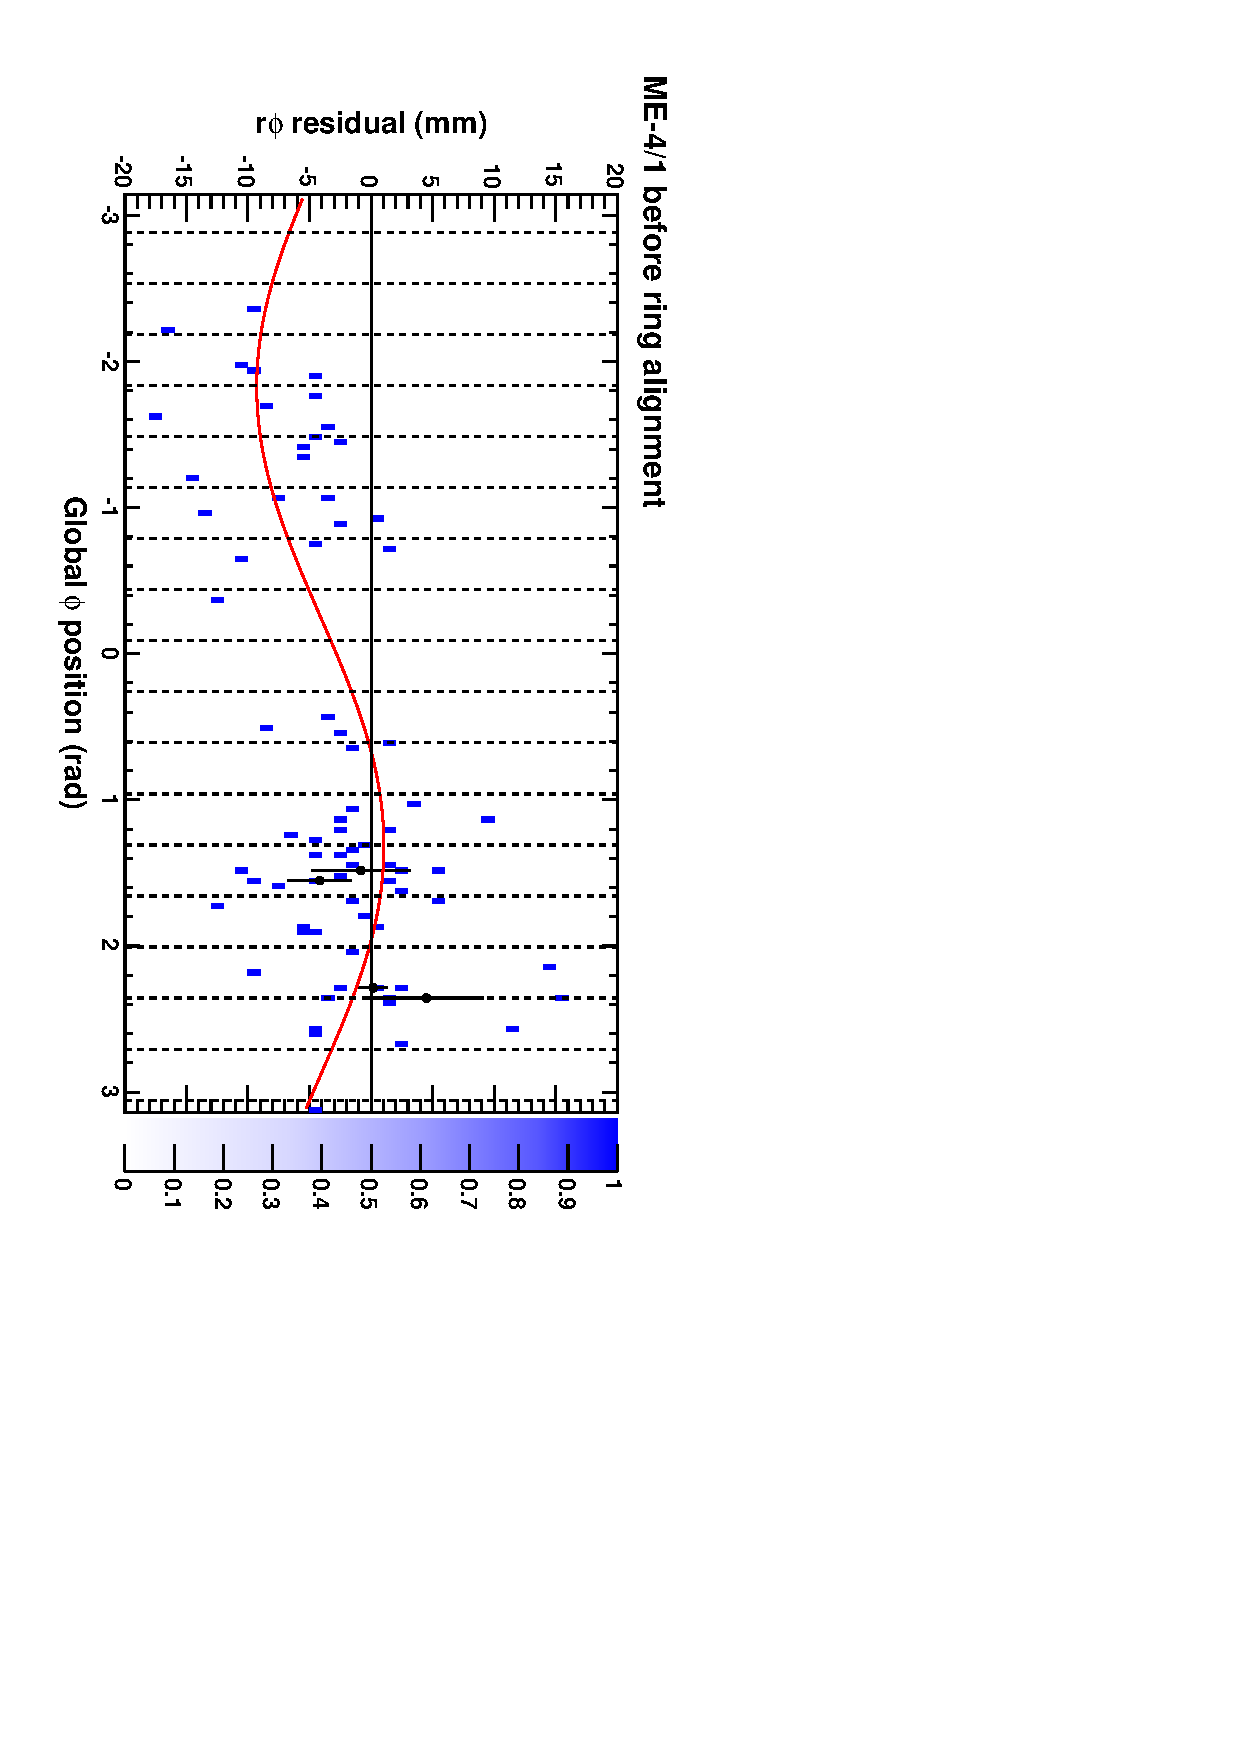
\includegraphics[height=\linewidth, angle=90]{ringfits_before/mem41.pdf}

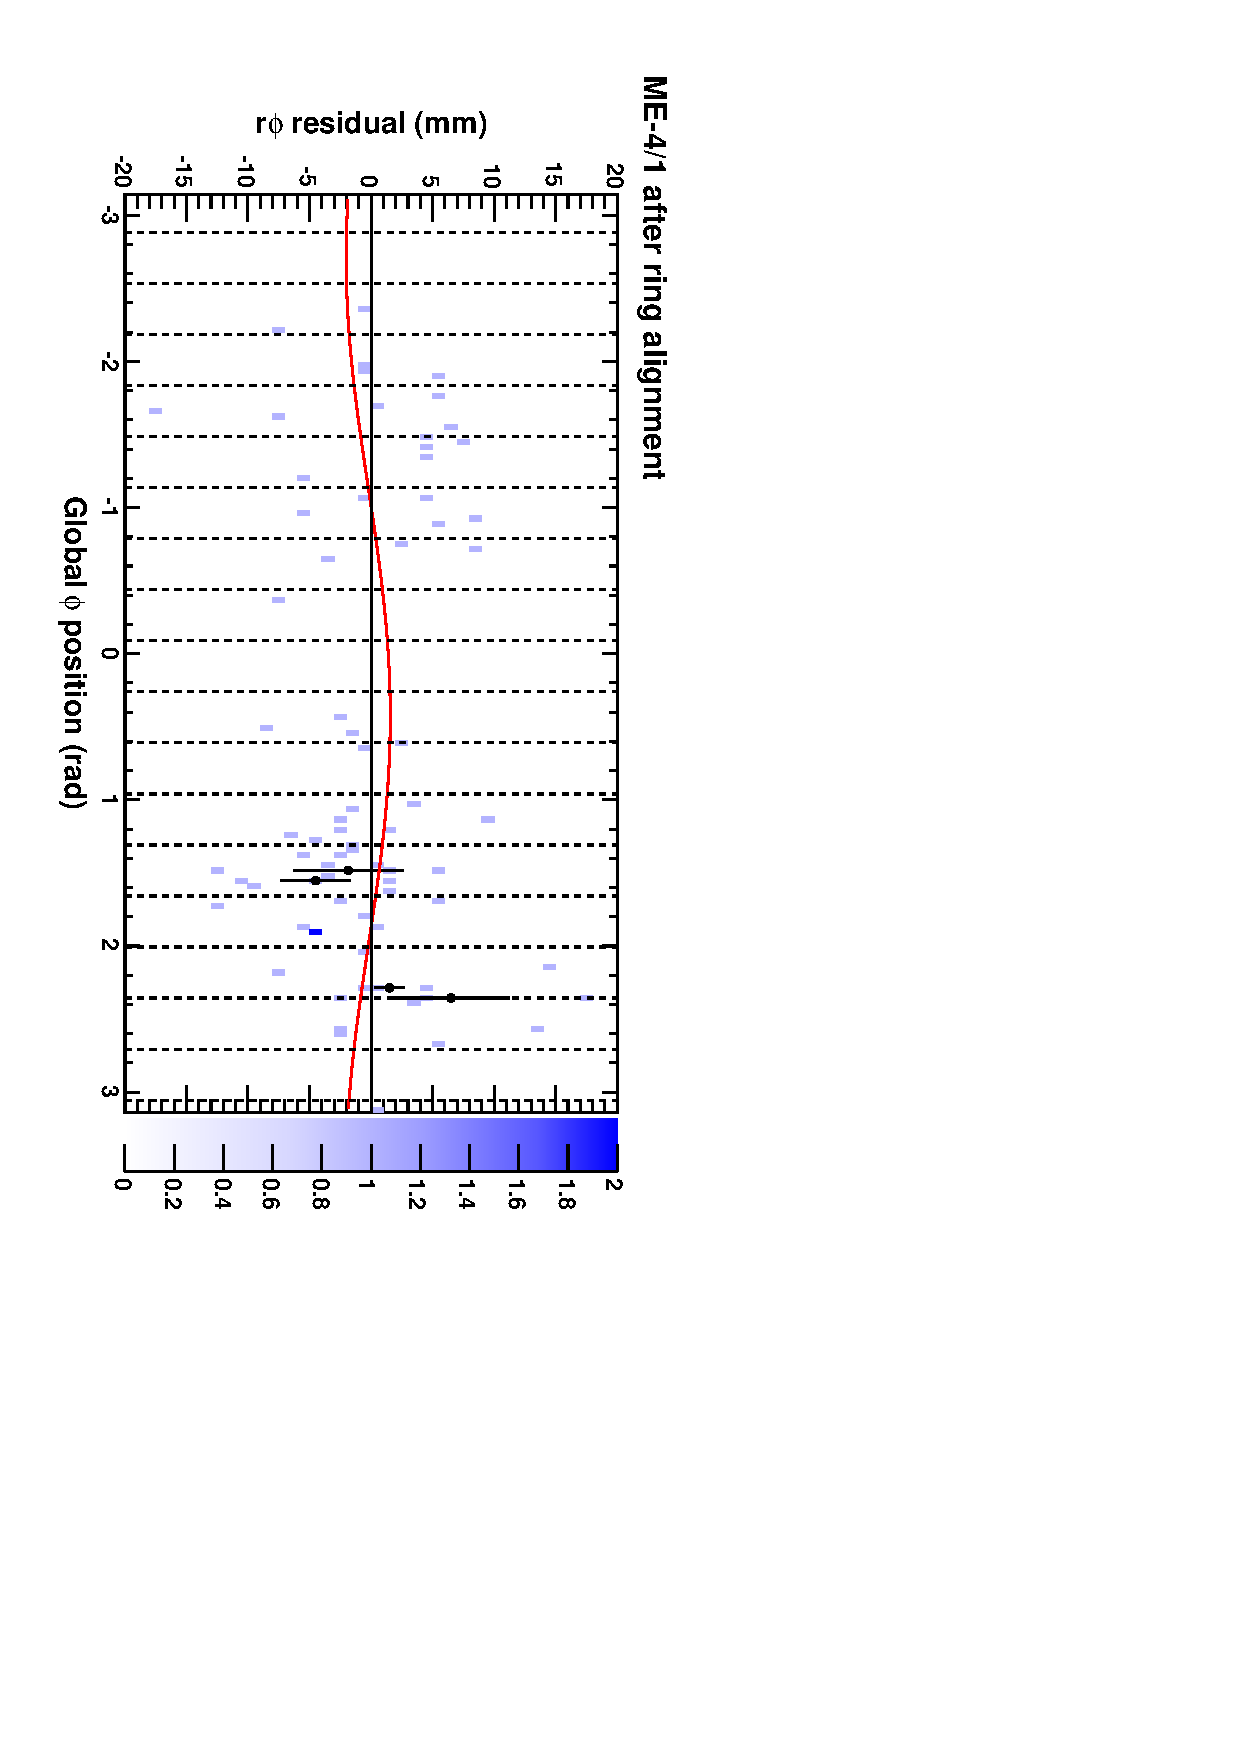
\includegraphics[height=\linewidth, angle=90]{ringfits_after/mem41.pdf}
\column{0.3\linewidth}
\begin{itemize}
\item Color scale is 2-D plot
\item Black points are a profile (averages in vertical bins)
\item Red line is fit to 2-D data
\end{itemize}
\end{columns}
\end{frame}

\begin{frame}
\frametitle{Ring fits: ME$-$3/2}
\vfill
\begin{columns}
\column{0.7\linewidth}
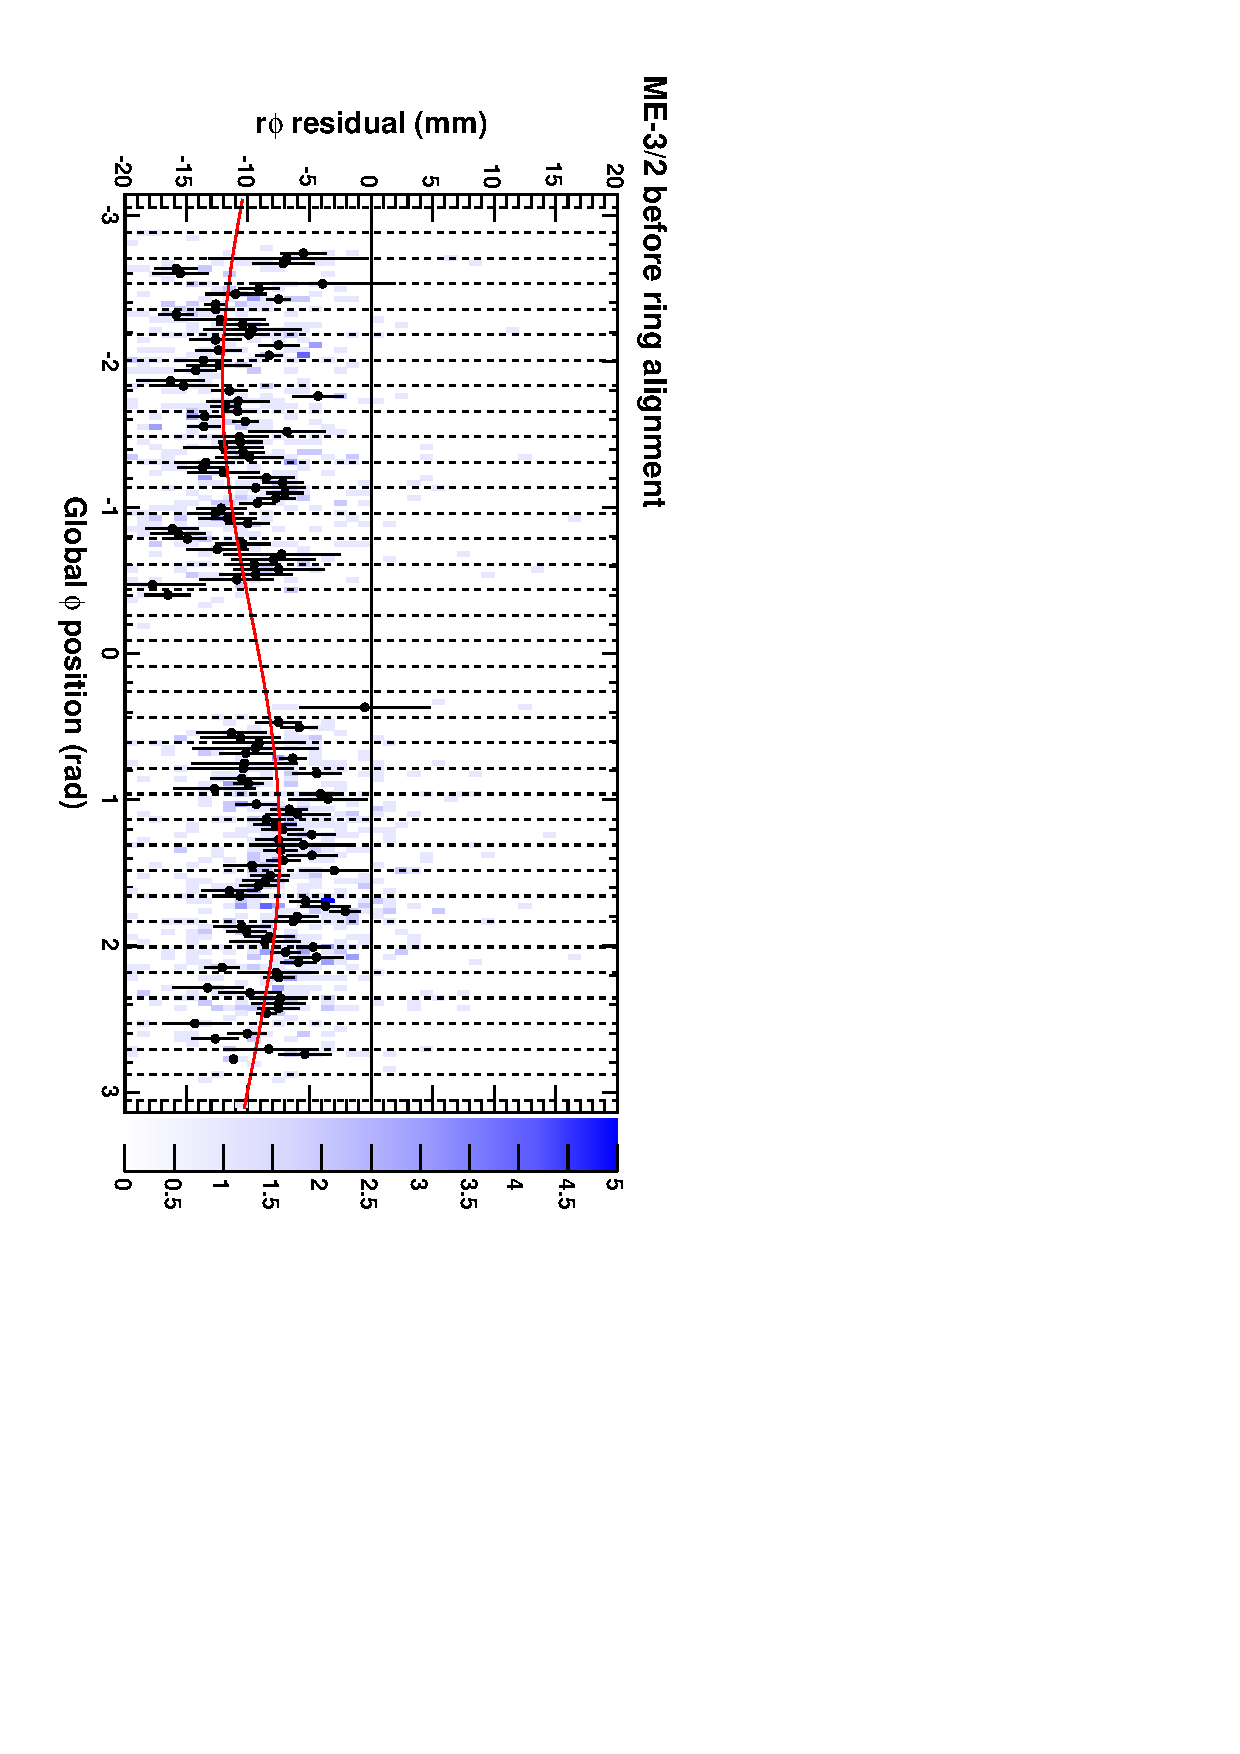
\includegraphics[height=\linewidth, angle=90]{ringfits_before/mem32.pdf}

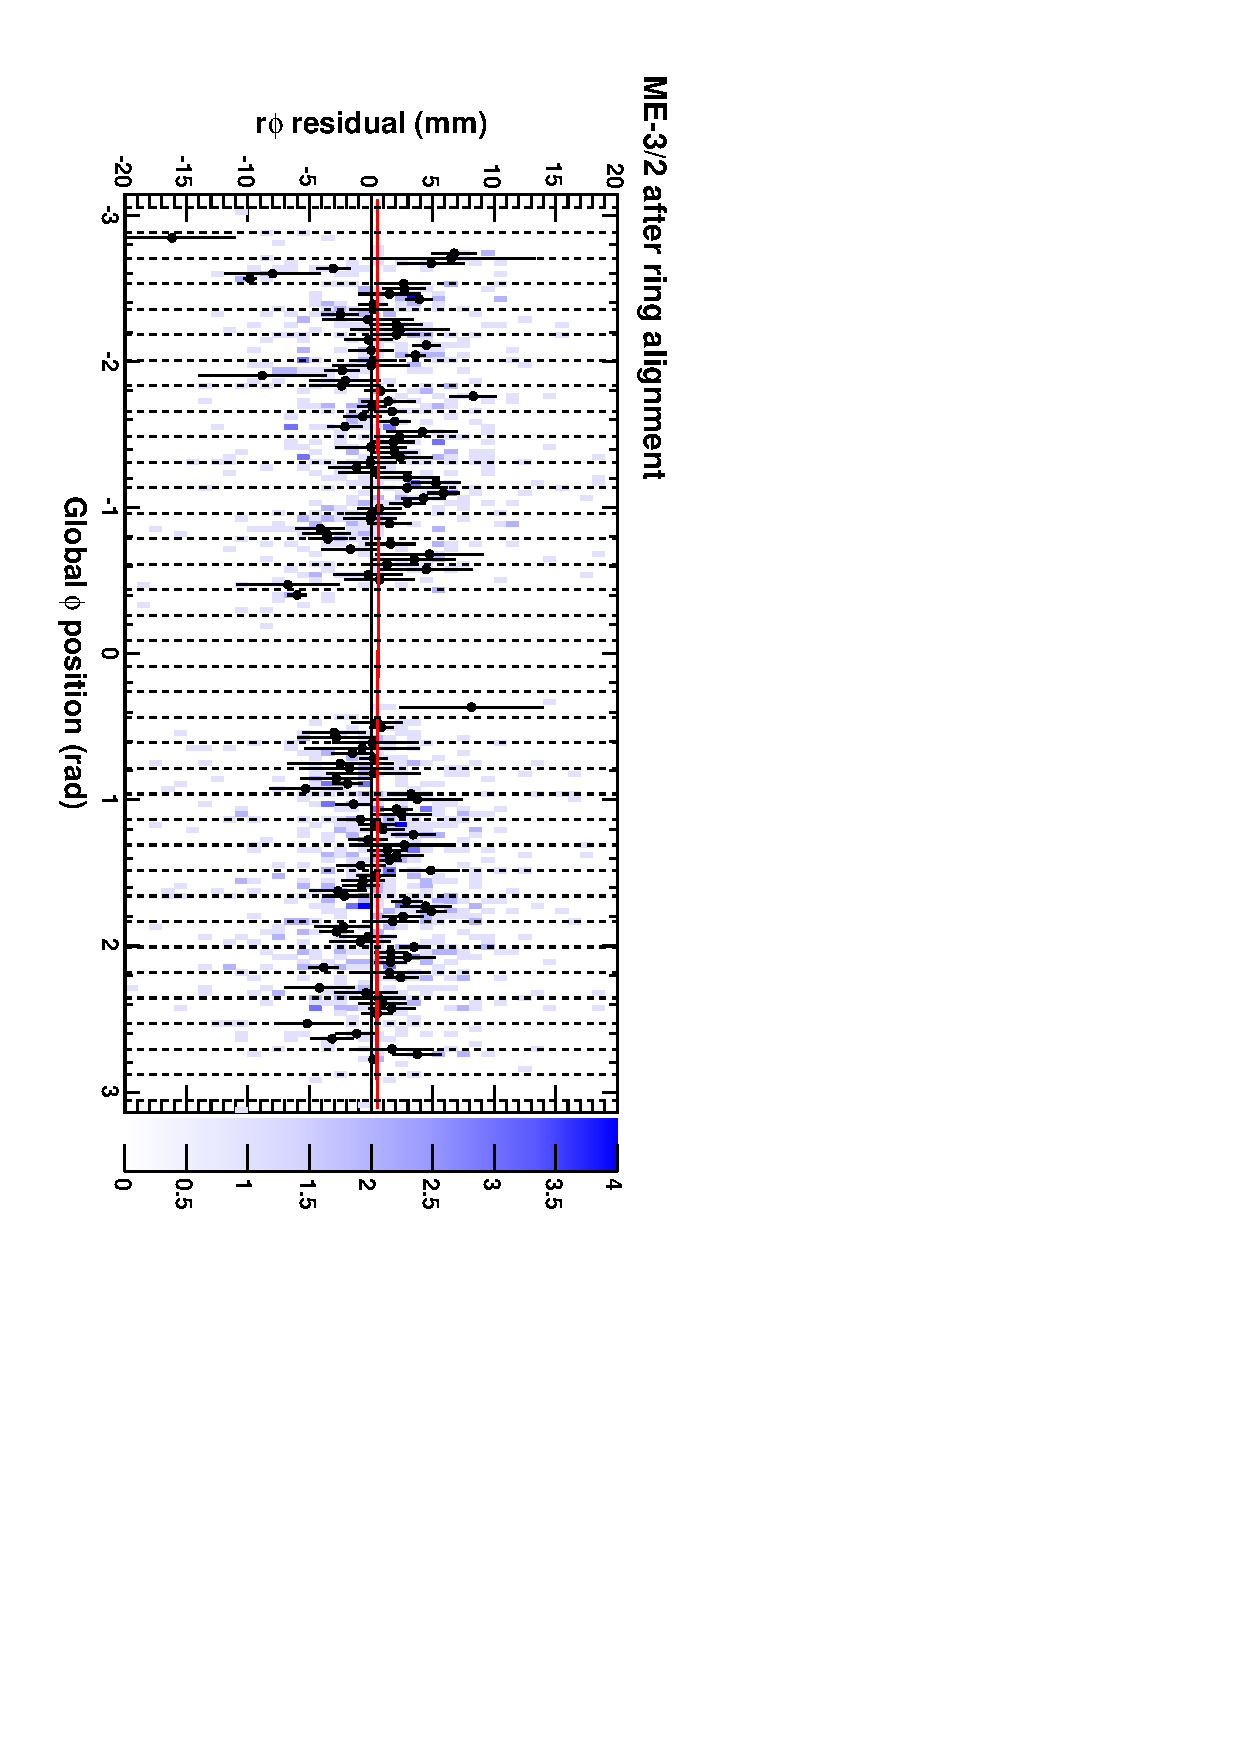
\includegraphics[height=\linewidth, angle=90]{ringfits_after/mem32.pdf}
\column{0.3\linewidth}
\begin{itemize}
\item Color scale is 2-D plot
\item Black points are a profile (averages in vertical bins)
\item Red line is fit to 2-D data
\end{itemize}
\end{columns}
\end{frame}

\begin{frame}
\frametitle{Ring fits: ME$-$3/1}
\vfill
\begin{columns}
\column{0.7\linewidth}
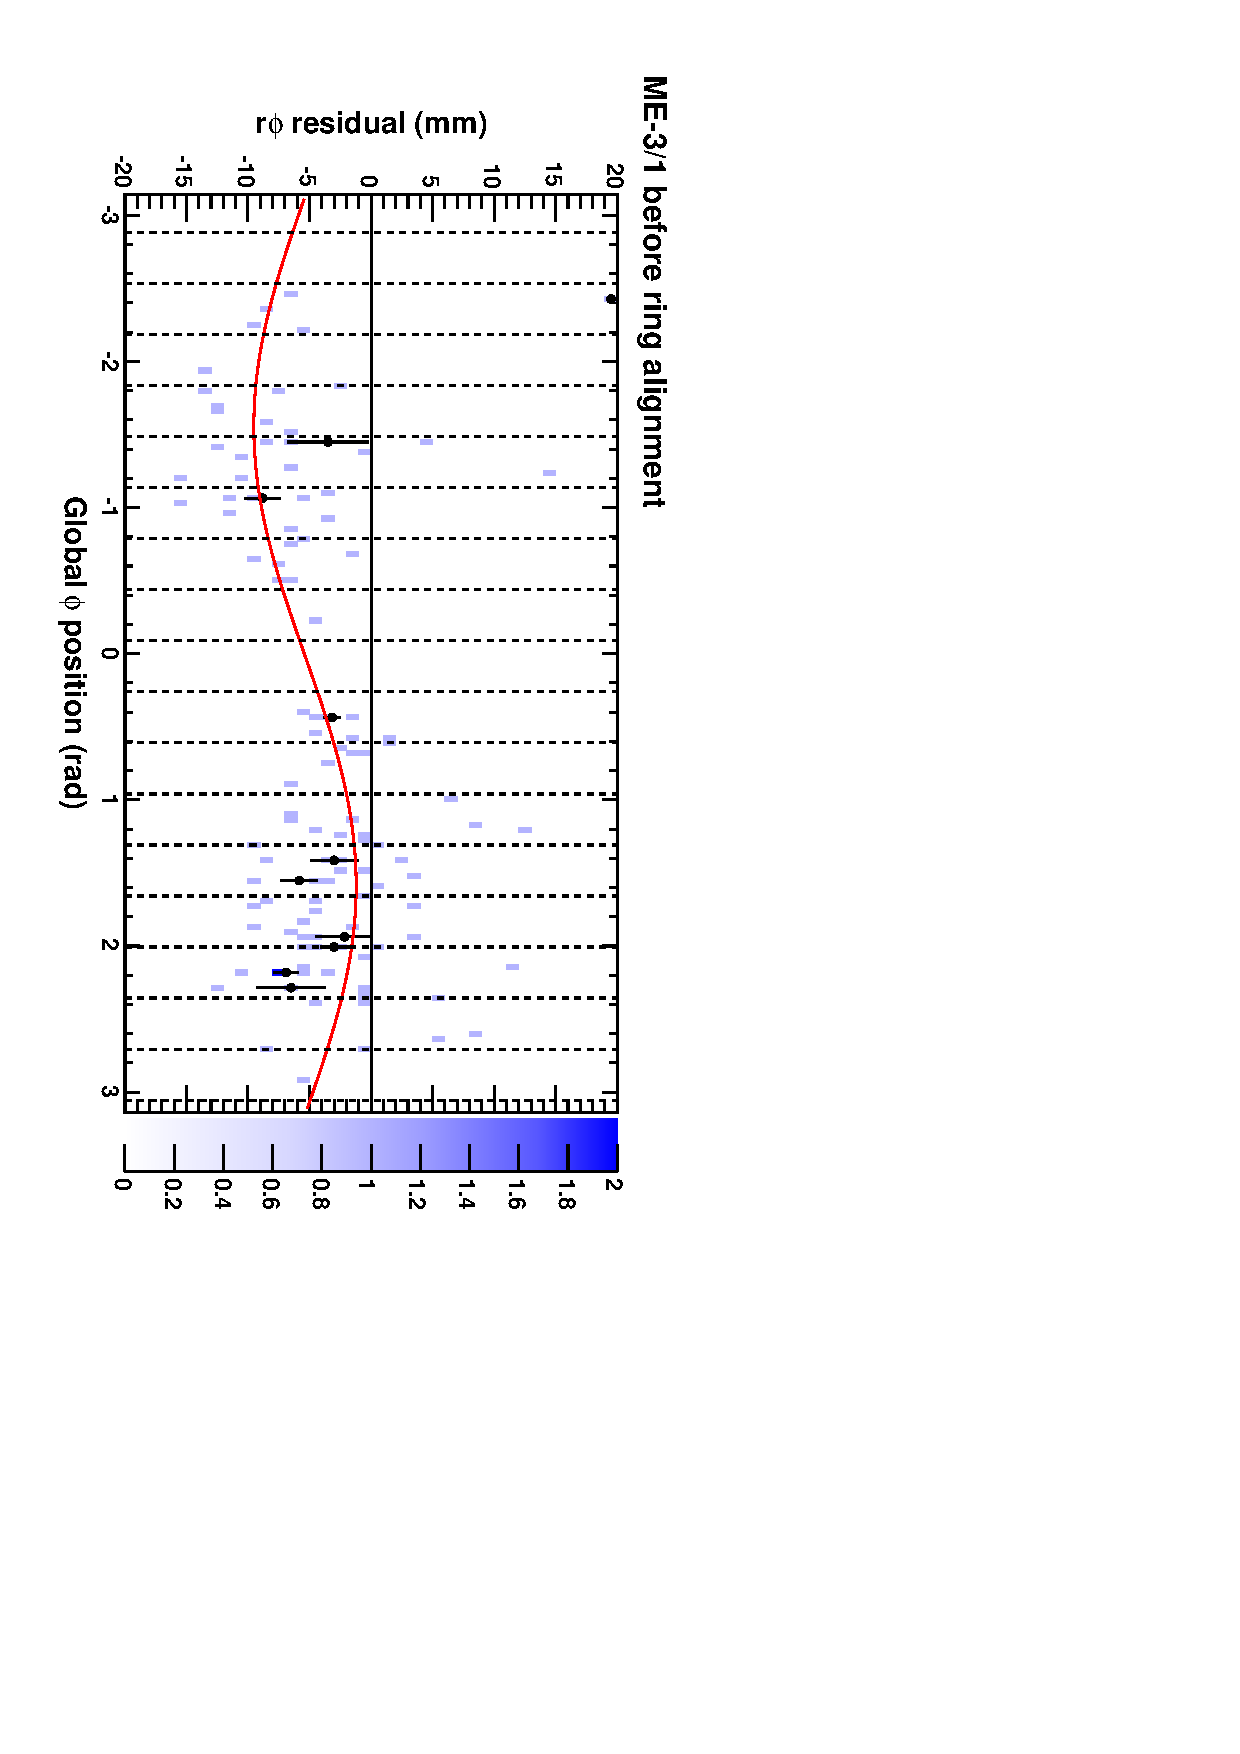
\includegraphics[height=\linewidth, angle=90]{ringfits_before/mem31.pdf}

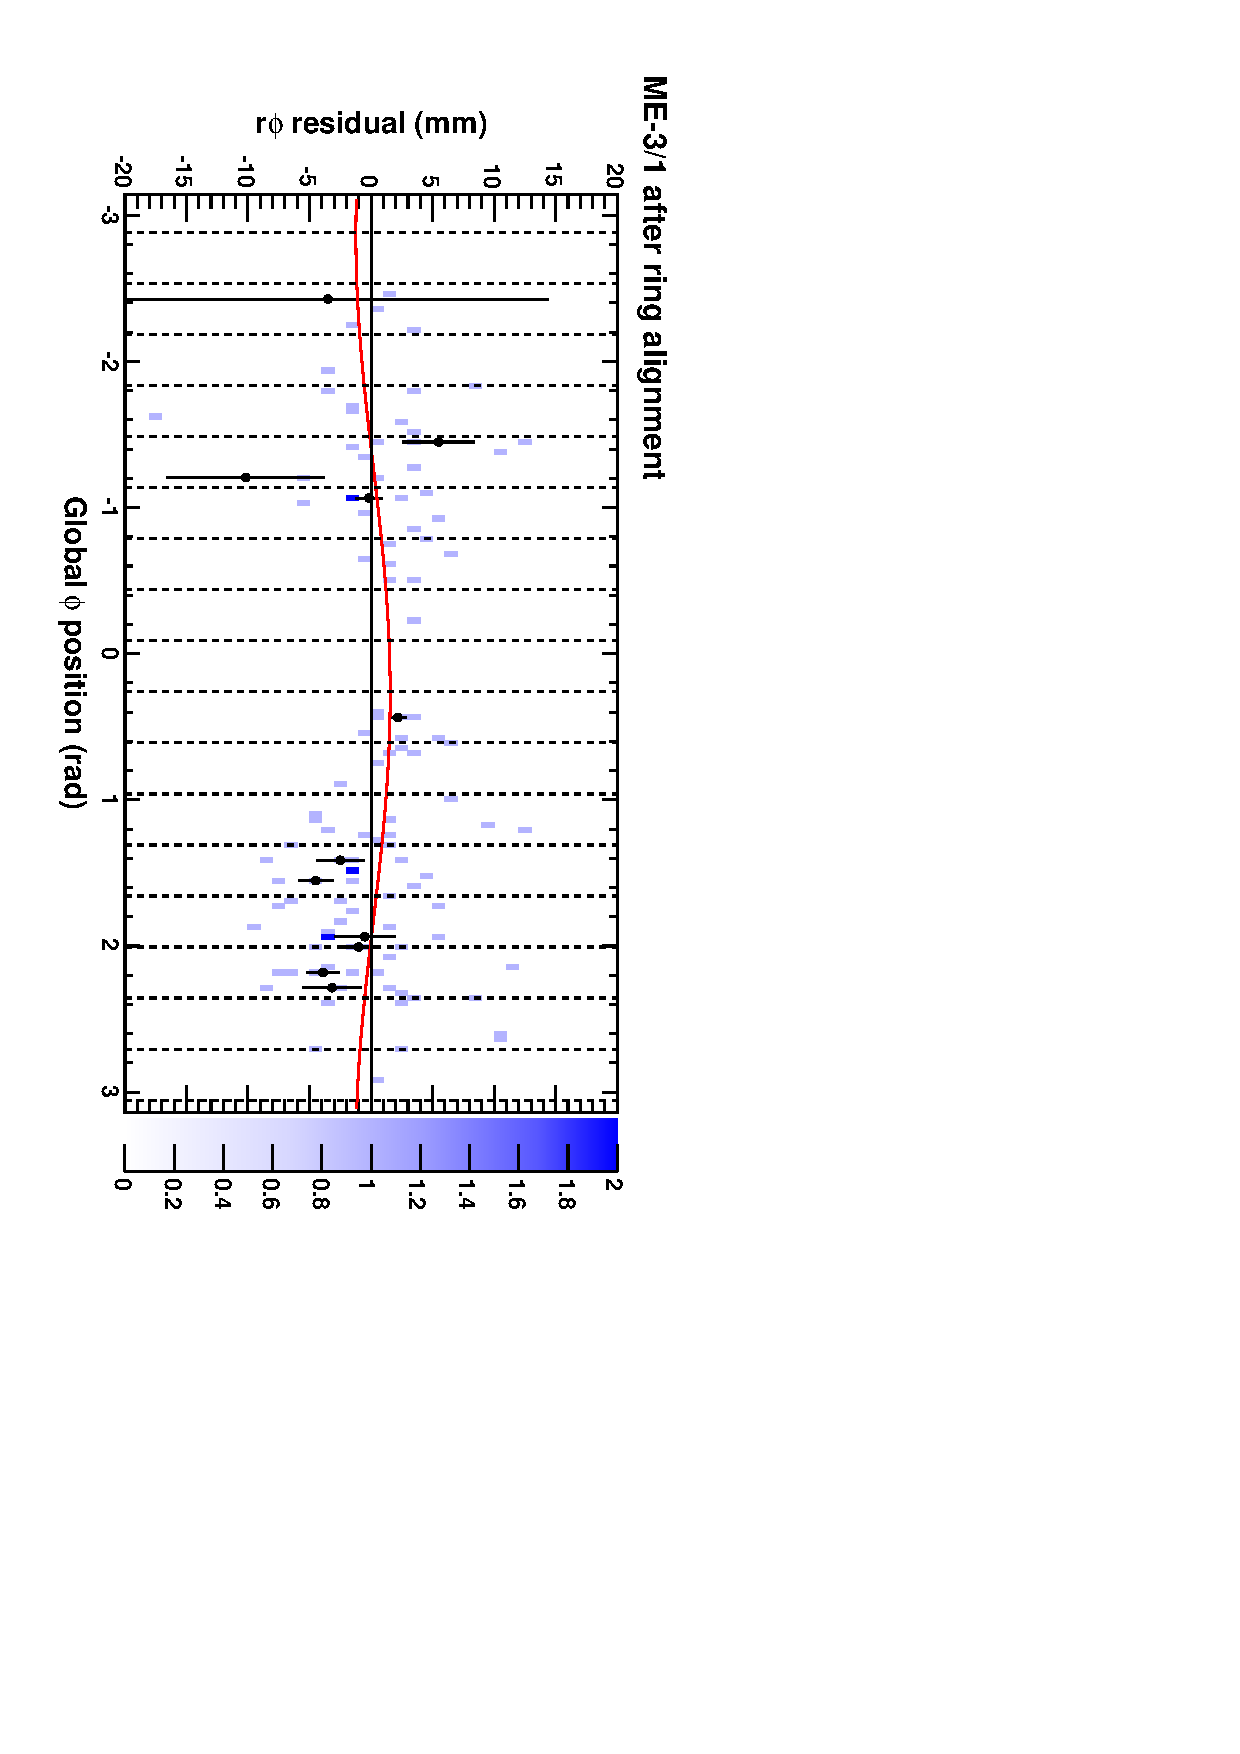
\includegraphics[height=\linewidth, angle=90]{ringfits_after/mem31.pdf}
\column{0.3\linewidth}
\begin{itemize}
\item Color scale is 2-D plot
\item Black points are a profile (averages in vertical bins)
\item Red line is fit to 2-D data
\end{itemize}
\end{columns}
\end{frame}

\begin{frame}
\frametitle{Ring fits: ME$-$2/2}
\vfill
\begin{columns}
\column{0.7\linewidth}
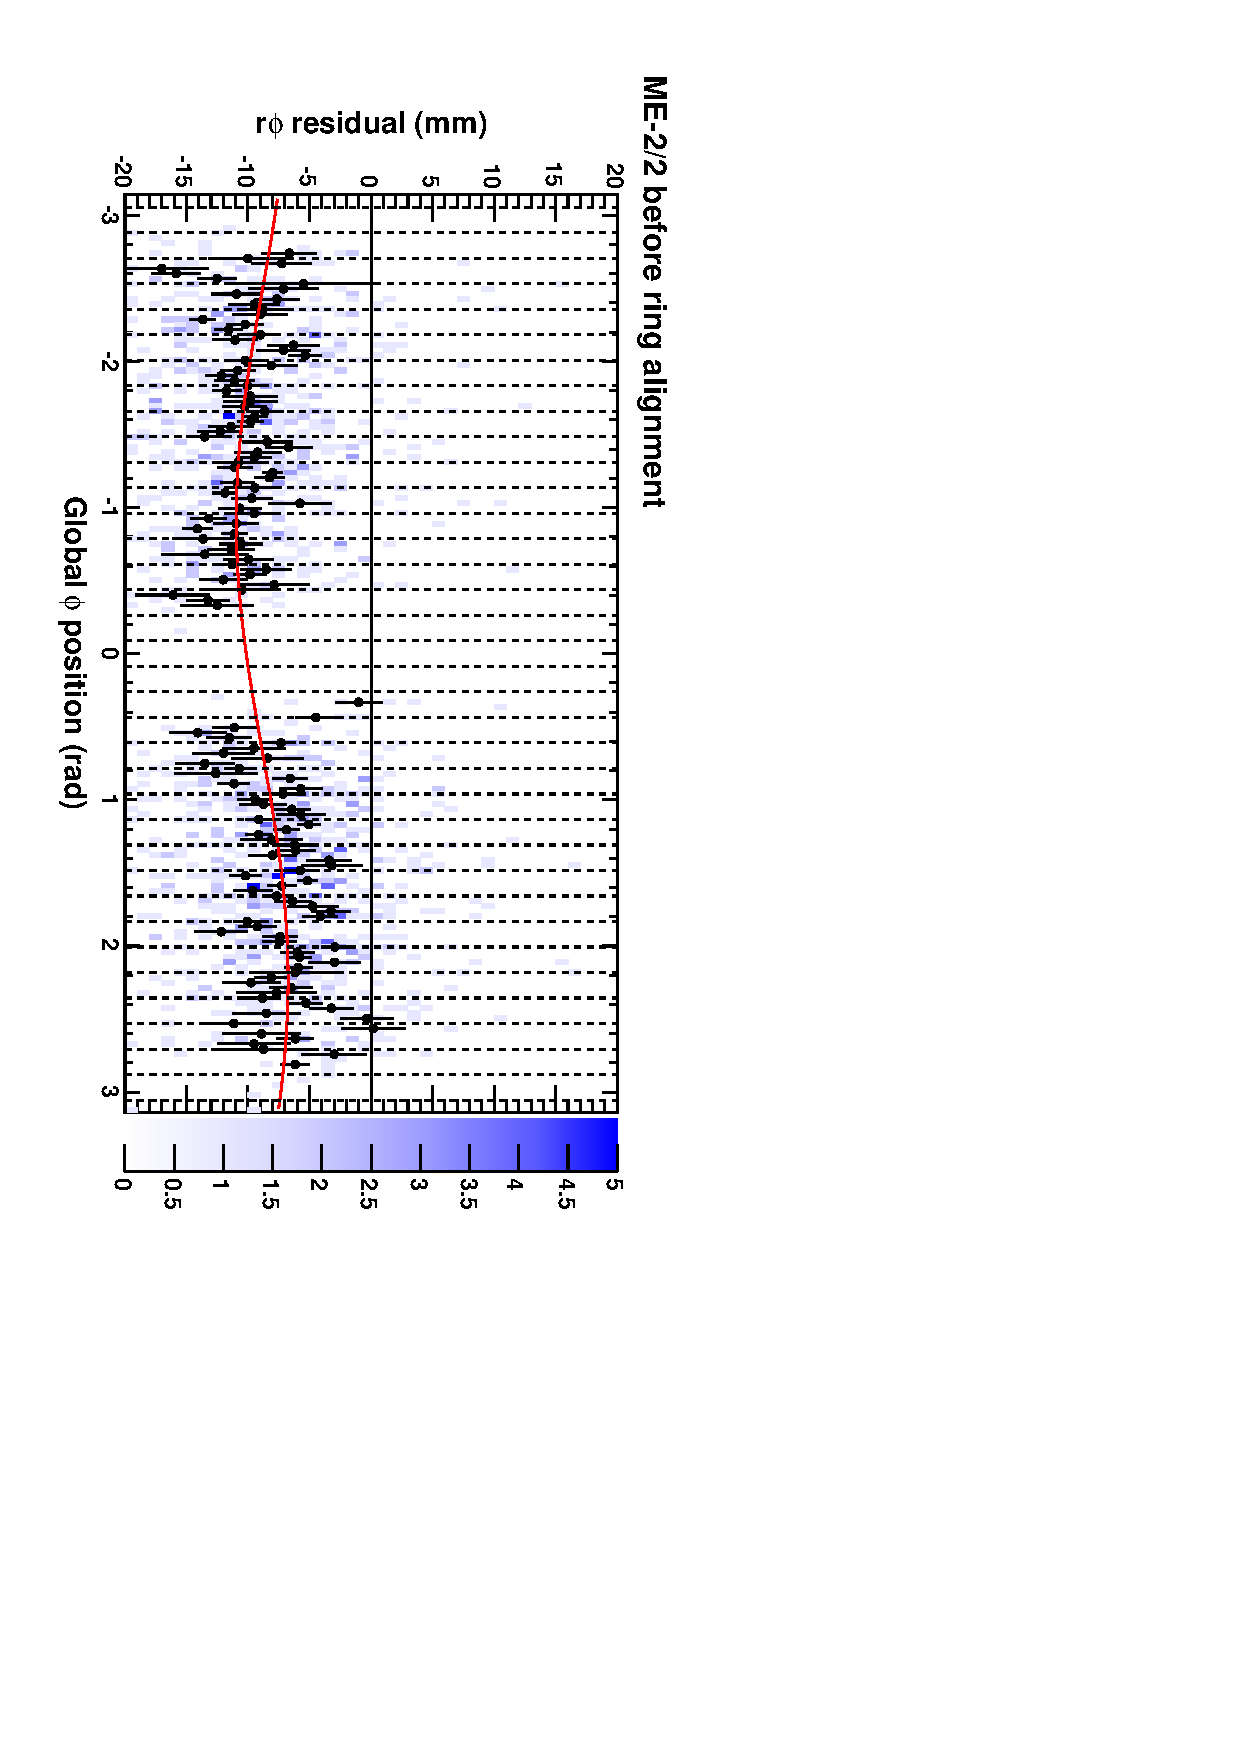
\includegraphics[height=\linewidth, angle=90]{ringfits_before/mem22.pdf}

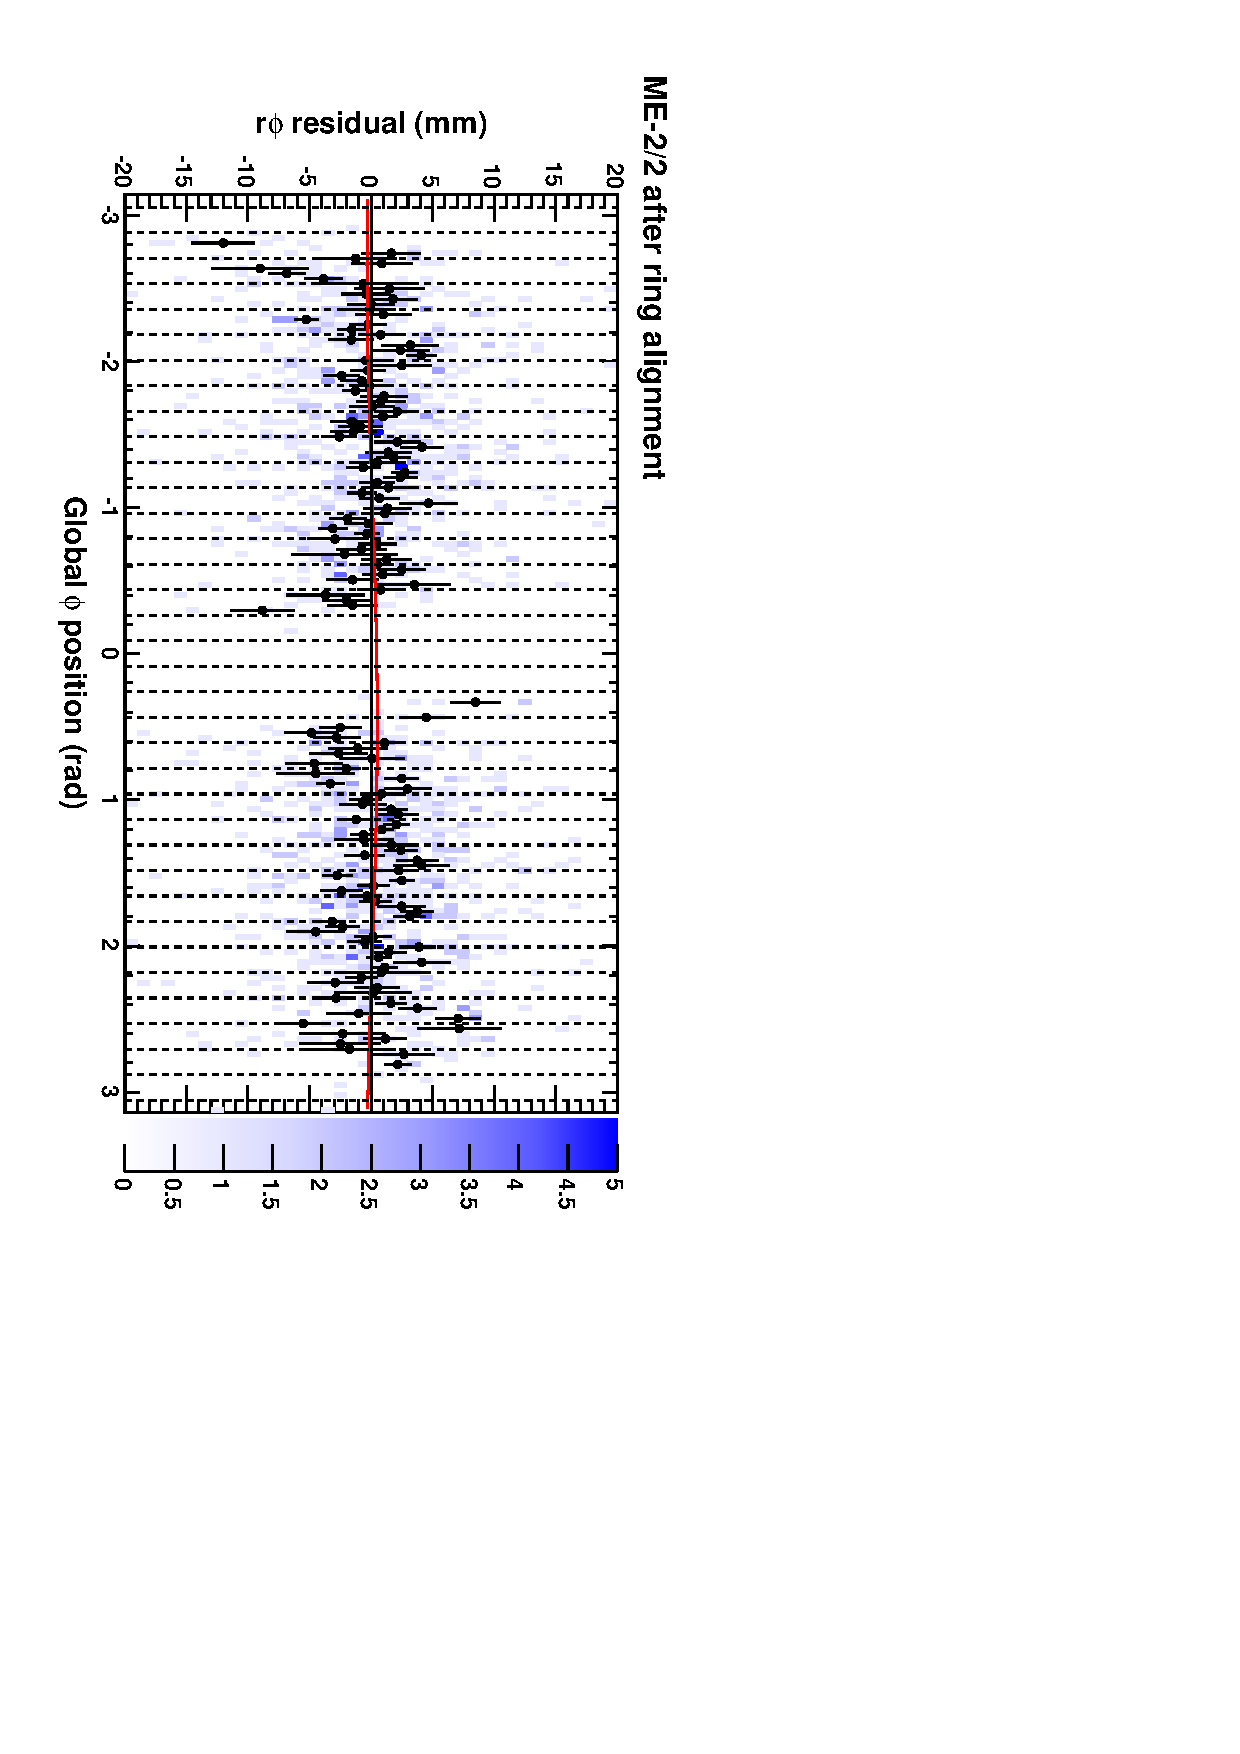
\includegraphics[height=\linewidth, angle=90]{ringfits_after/mem22.pdf}
\column{0.3\linewidth}
\begin{itemize}
\item Color scale is 2-D plot
\item Black points are a profile (averages in vertical bins)
\item Red line is fit to 2-D data
\end{itemize}
\end{columns}
\end{frame}

\begin{frame}
\frametitle{Ring fits: ME$-$2/1}
\vfill
\begin{columns}
\column{0.7\linewidth}
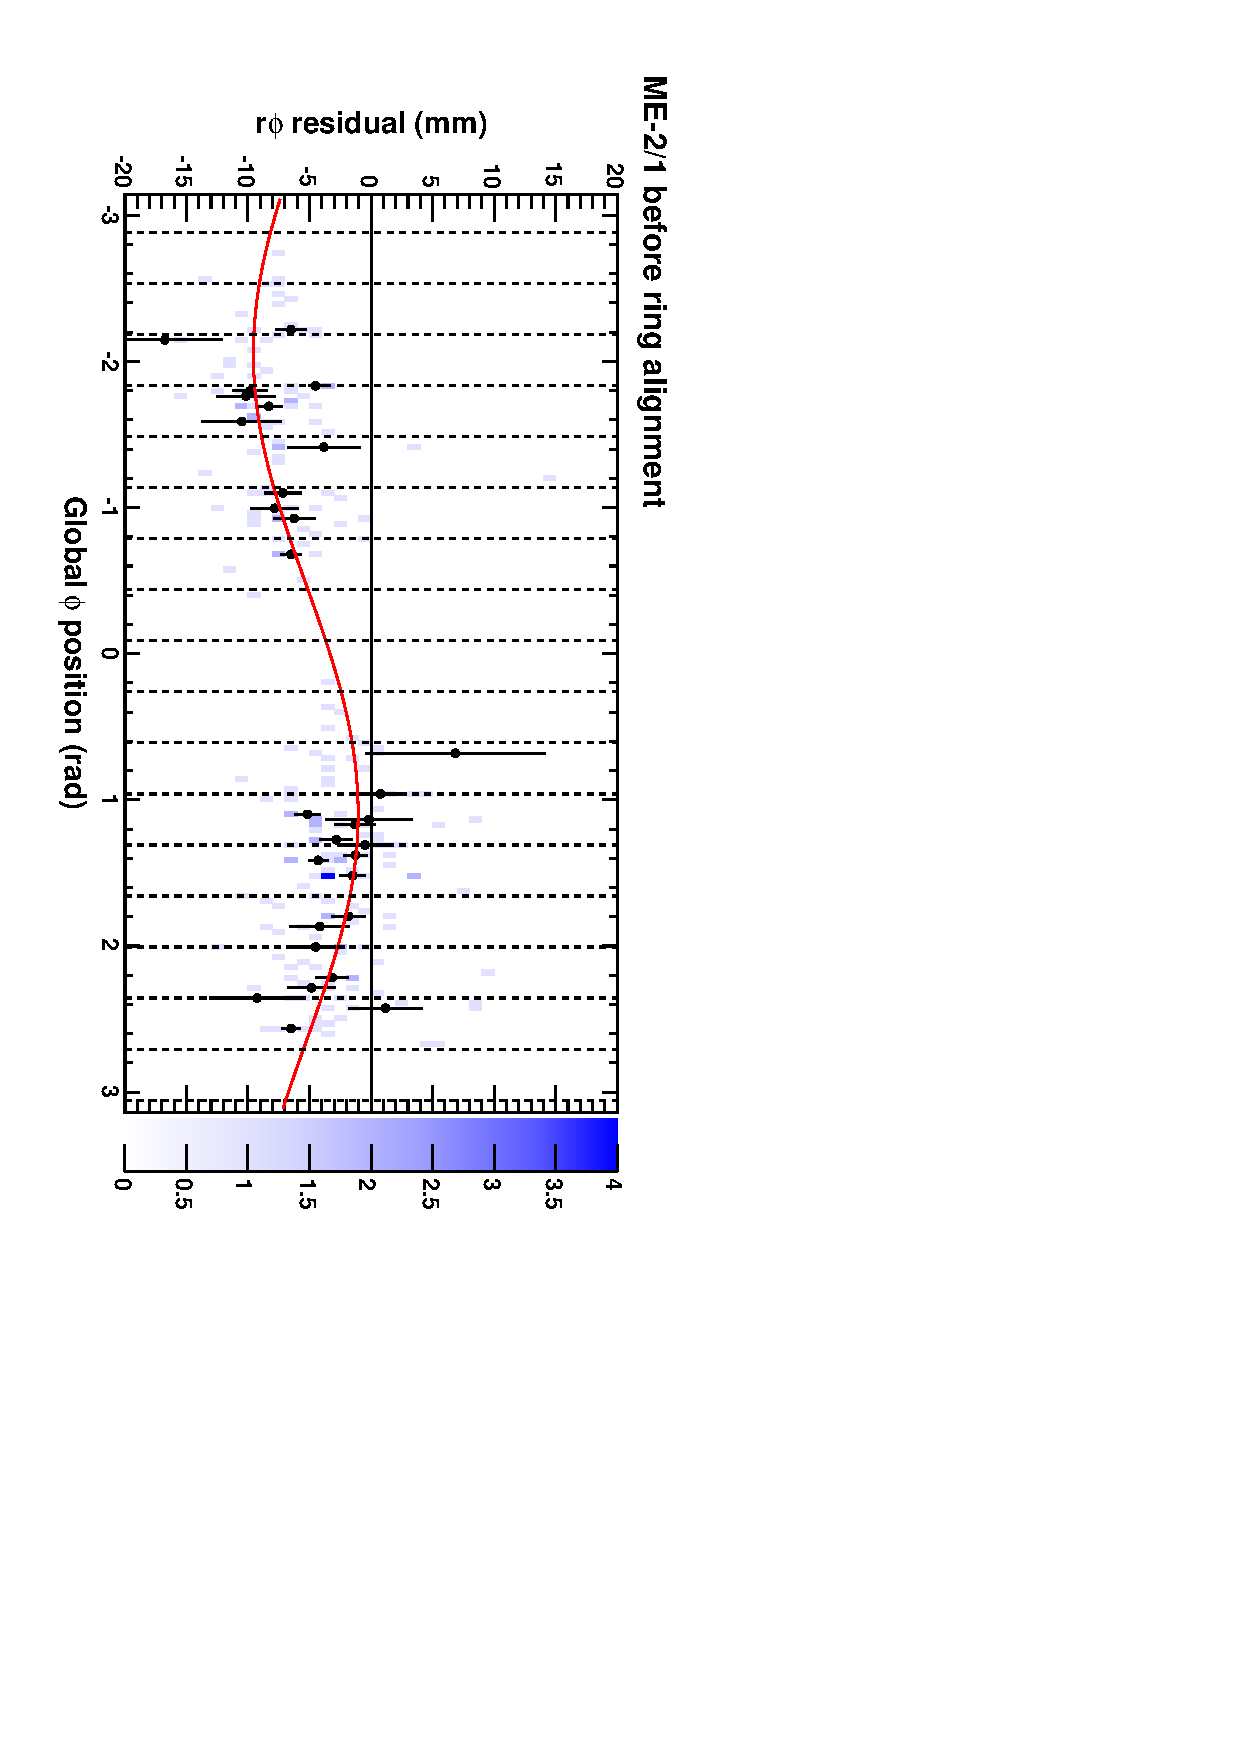
\includegraphics[height=\linewidth, angle=90]{ringfits_before/mem21.pdf}

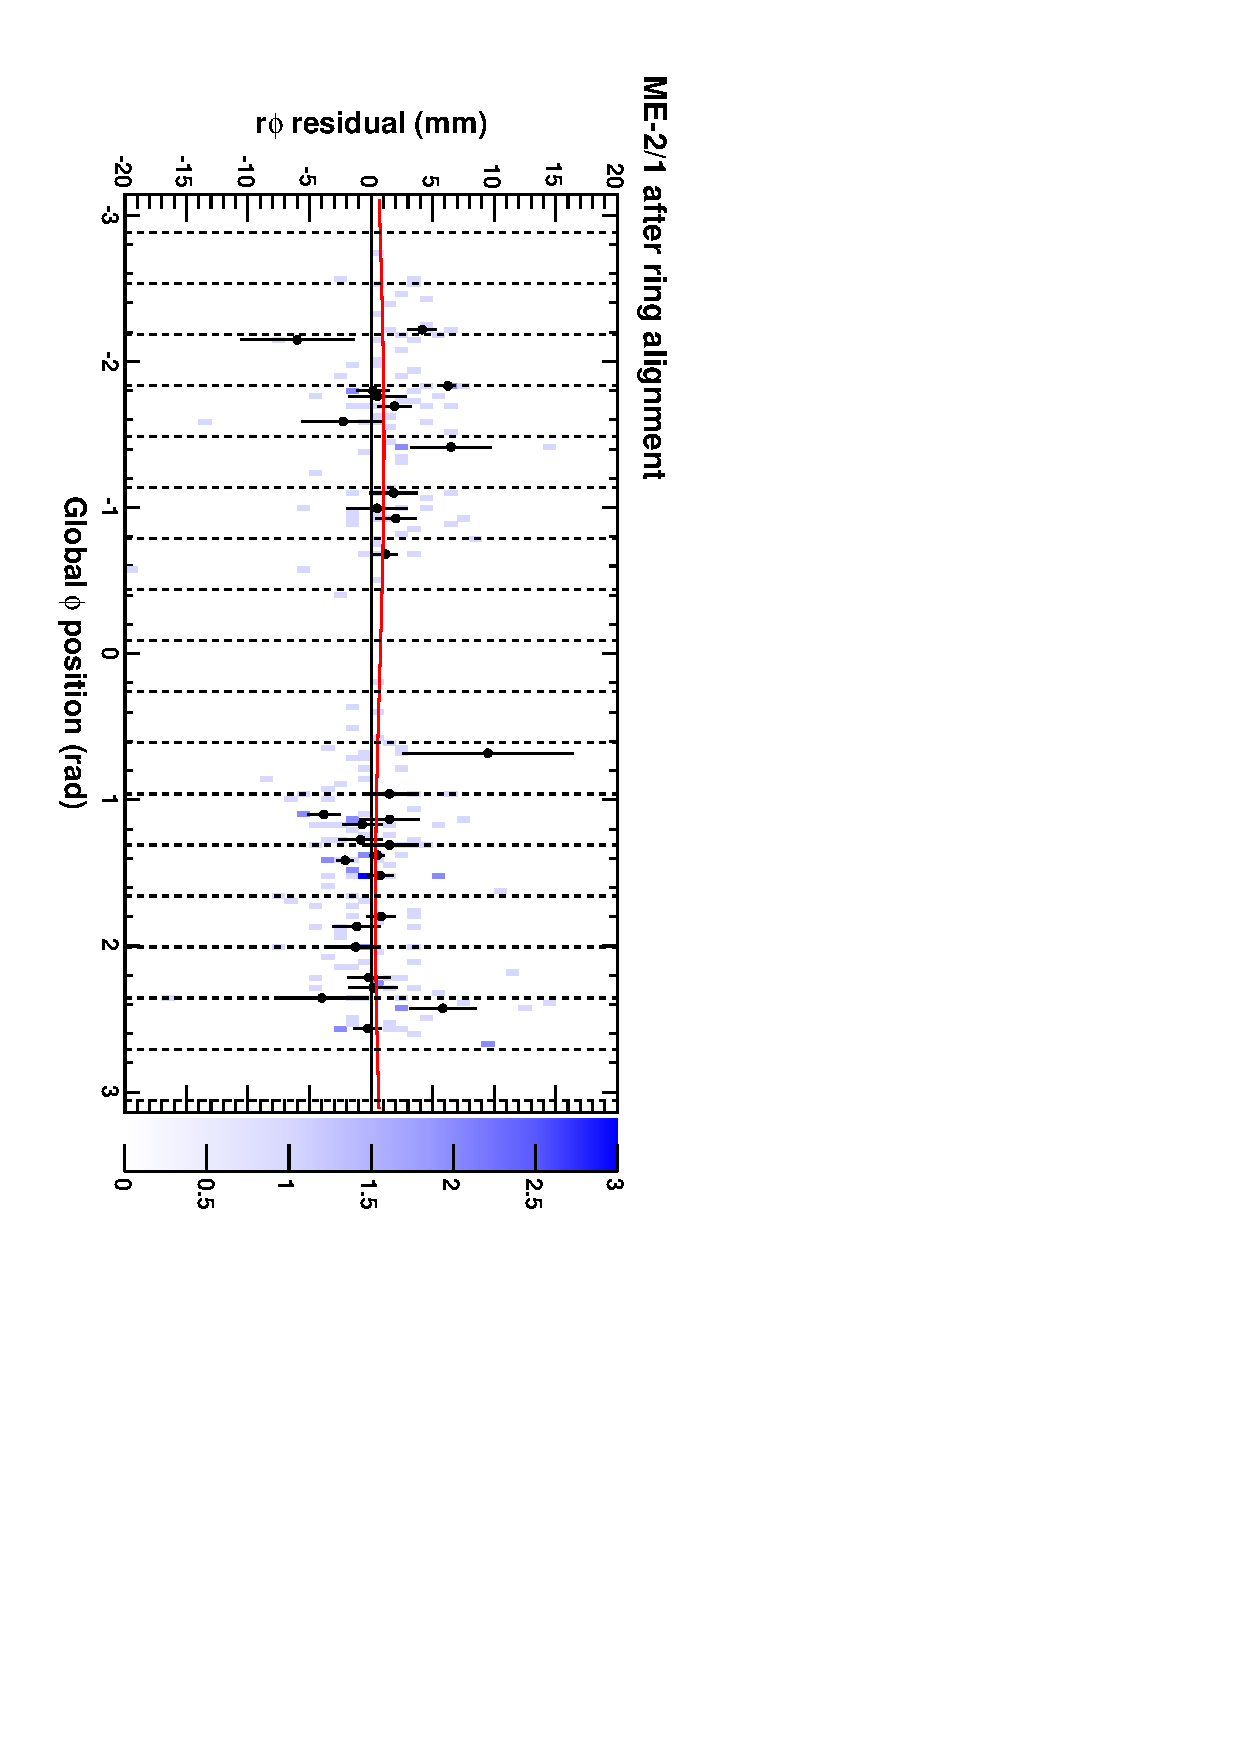
\includegraphics[height=\linewidth, angle=90]{ringfits_after/mem21.pdf}
\column{0.3\linewidth}
\begin{itemize}
\item Color scale is 2-D plot
\item Black points are a profile (averages in vertical bins)
\item Red line is fit to 2-D data
\end{itemize}
\end{columns}
\end{frame}

\begin{frame}
\frametitle{Ring fits: ME$-$1/3}
\vfill
\begin{columns}
\column{0.7\linewidth}
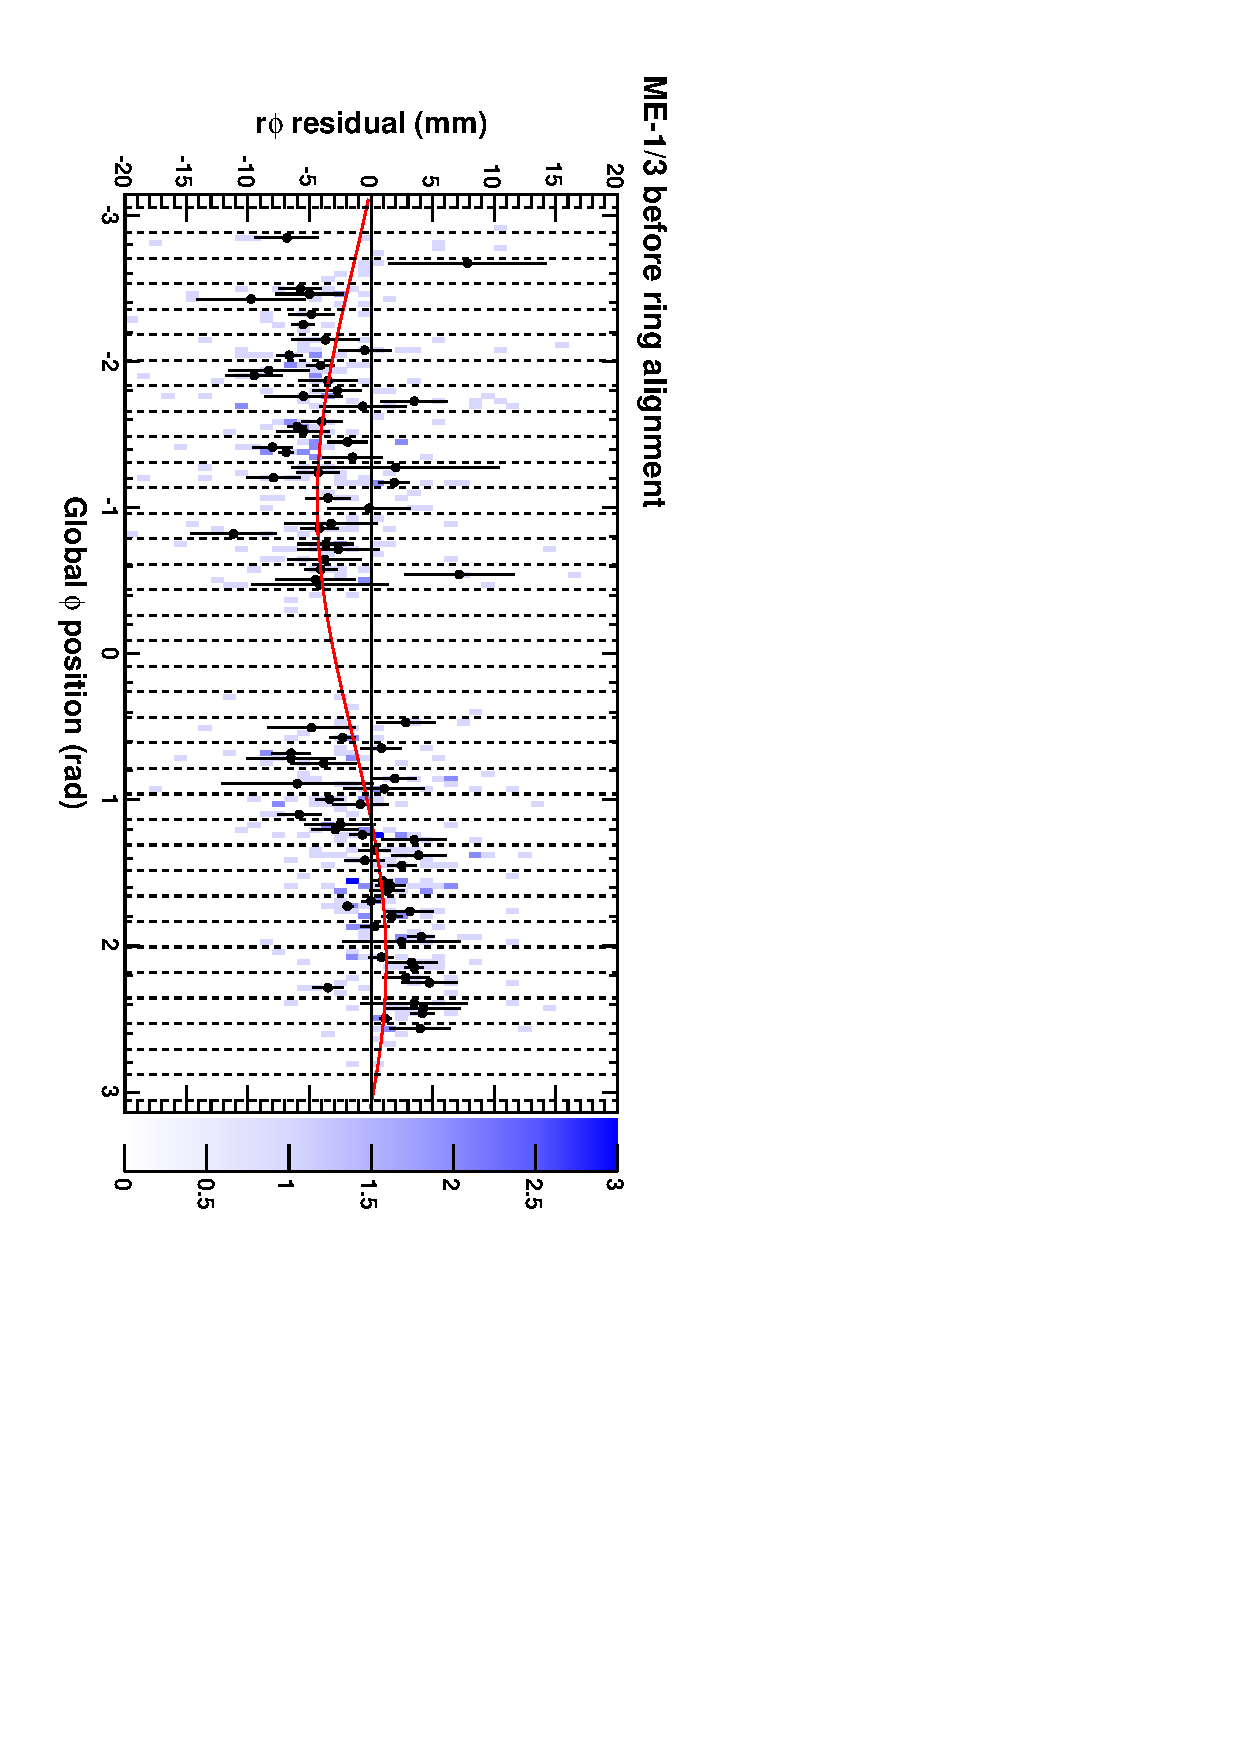
\includegraphics[height=\linewidth, angle=90]{ringfits_before/mem13.pdf}

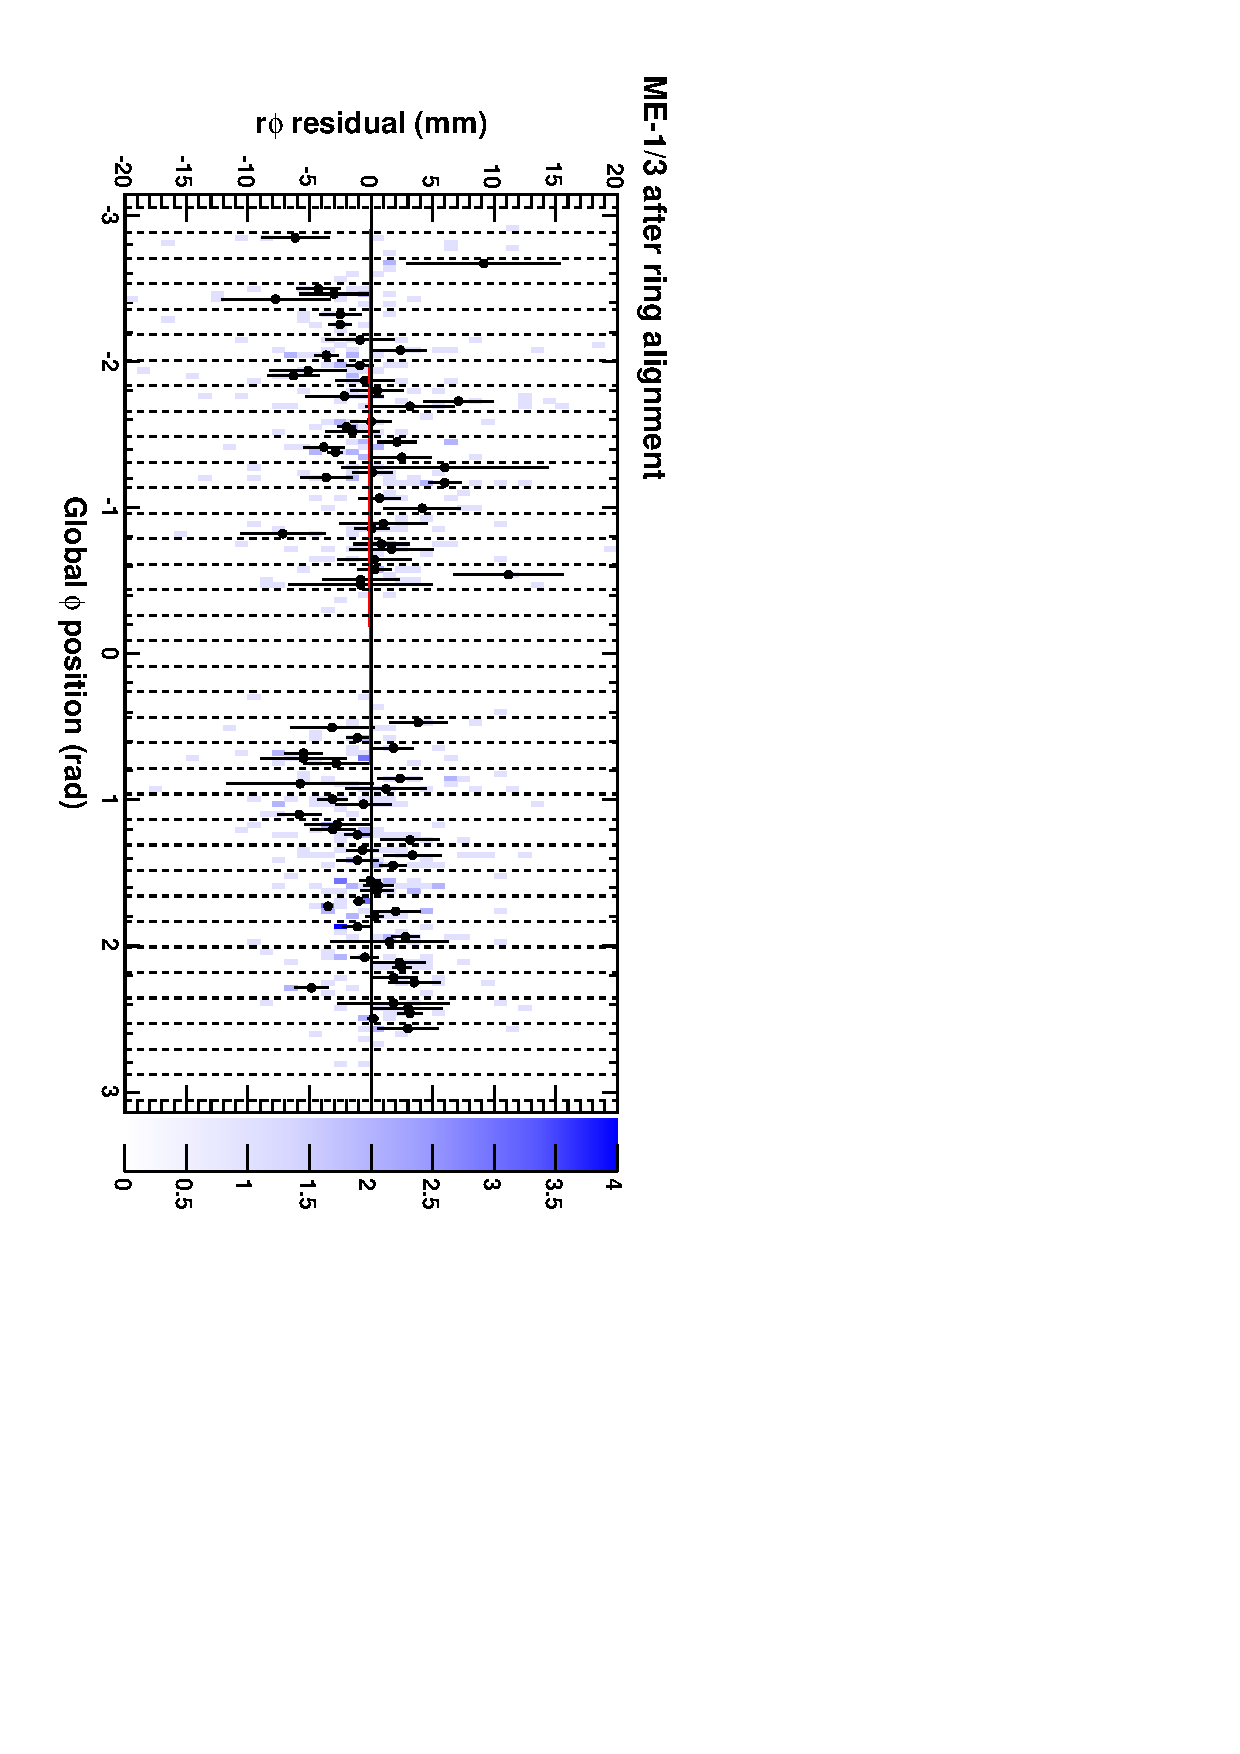
\includegraphics[height=\linewidth, angle=90]{ringfits_after/mem13.pdf}
\column{0.3\linewidth}
\begin{itemize}
\item Color scale is 2-D plot
\item Black points are a profile (averages in vertical bins)
\item Red line is fit to 2-D data
\end{itemize}
\end{columns}
\end{frame}

\begin{frame}
\frametitle{Ring fits: ME$-$1/2}
\vfill
\begin{columns}
\column{0.7\linewidth}
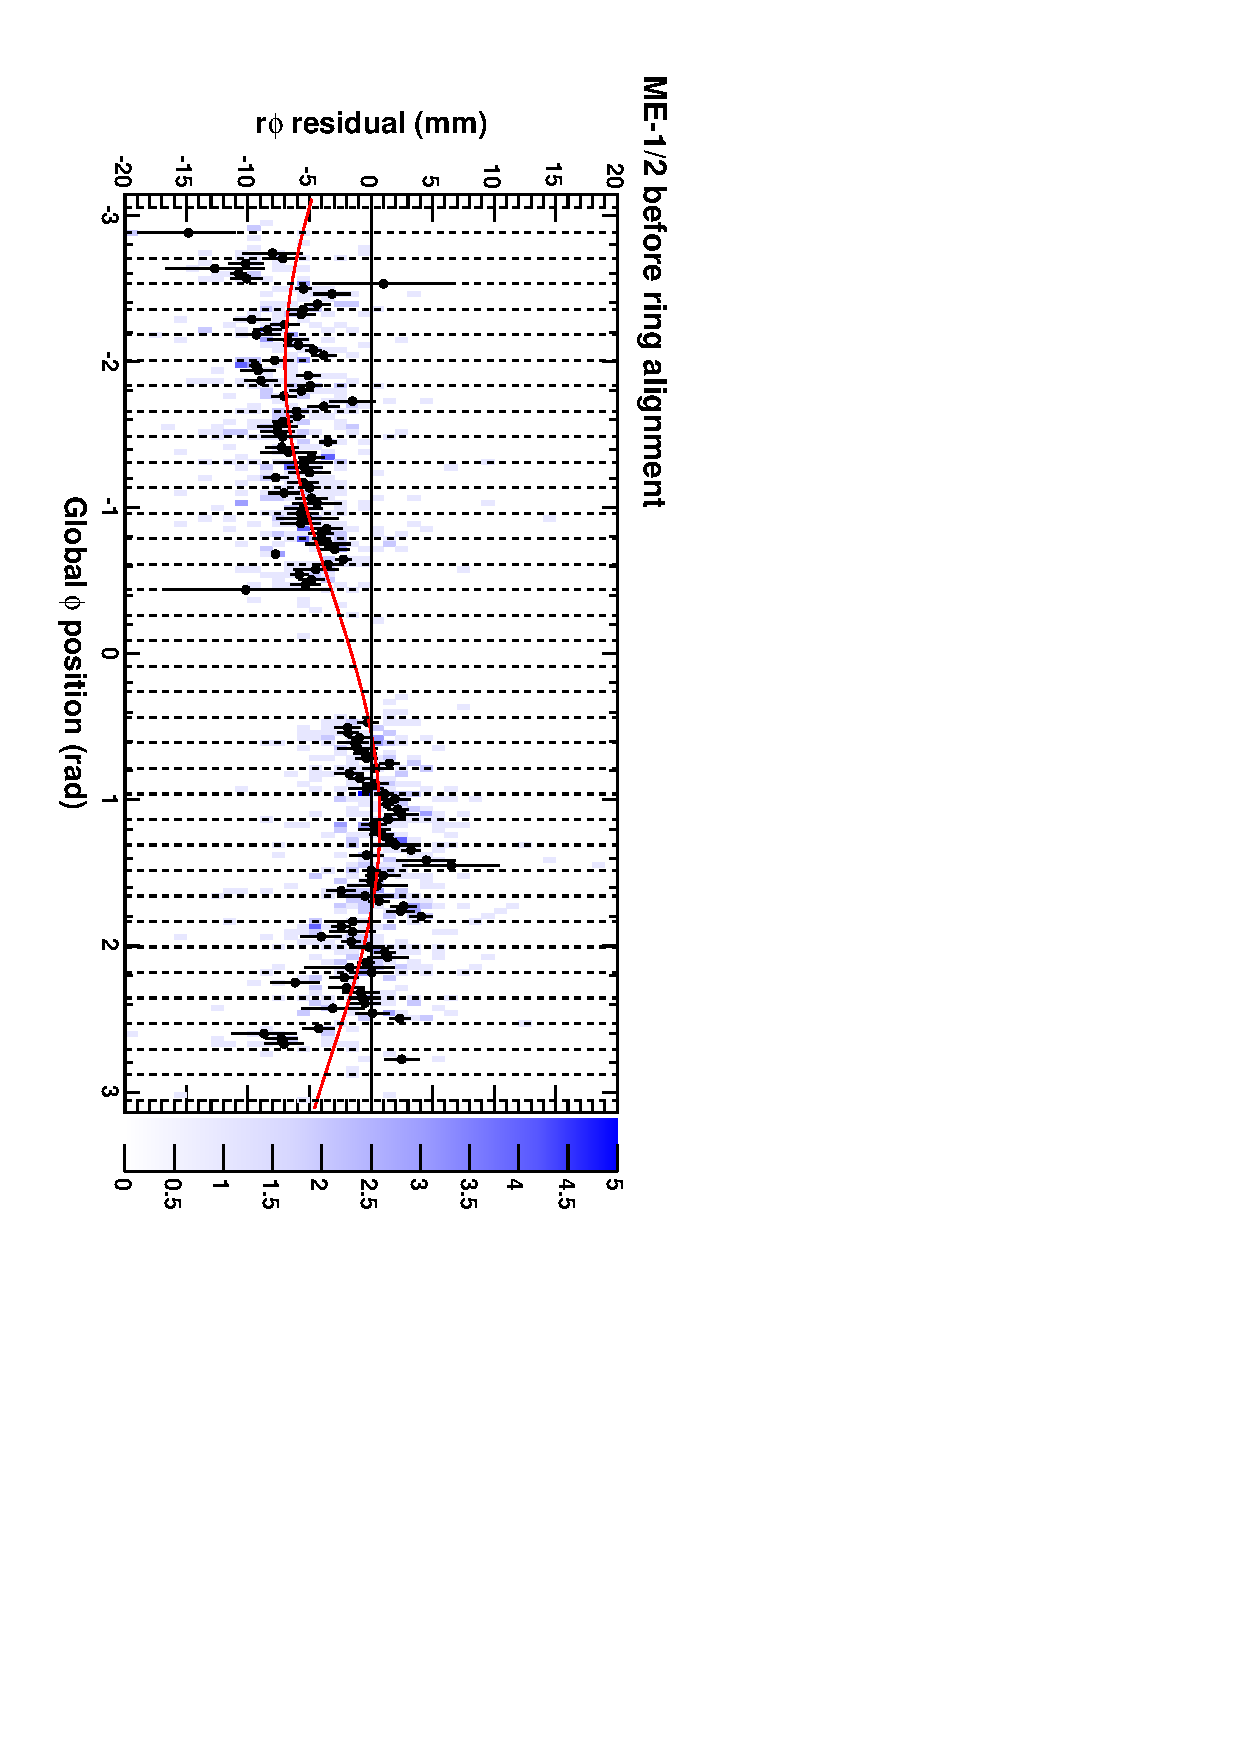
\includegraphics[height=\linewidth, angle=90]{ringfits_before/mem12.pdf}

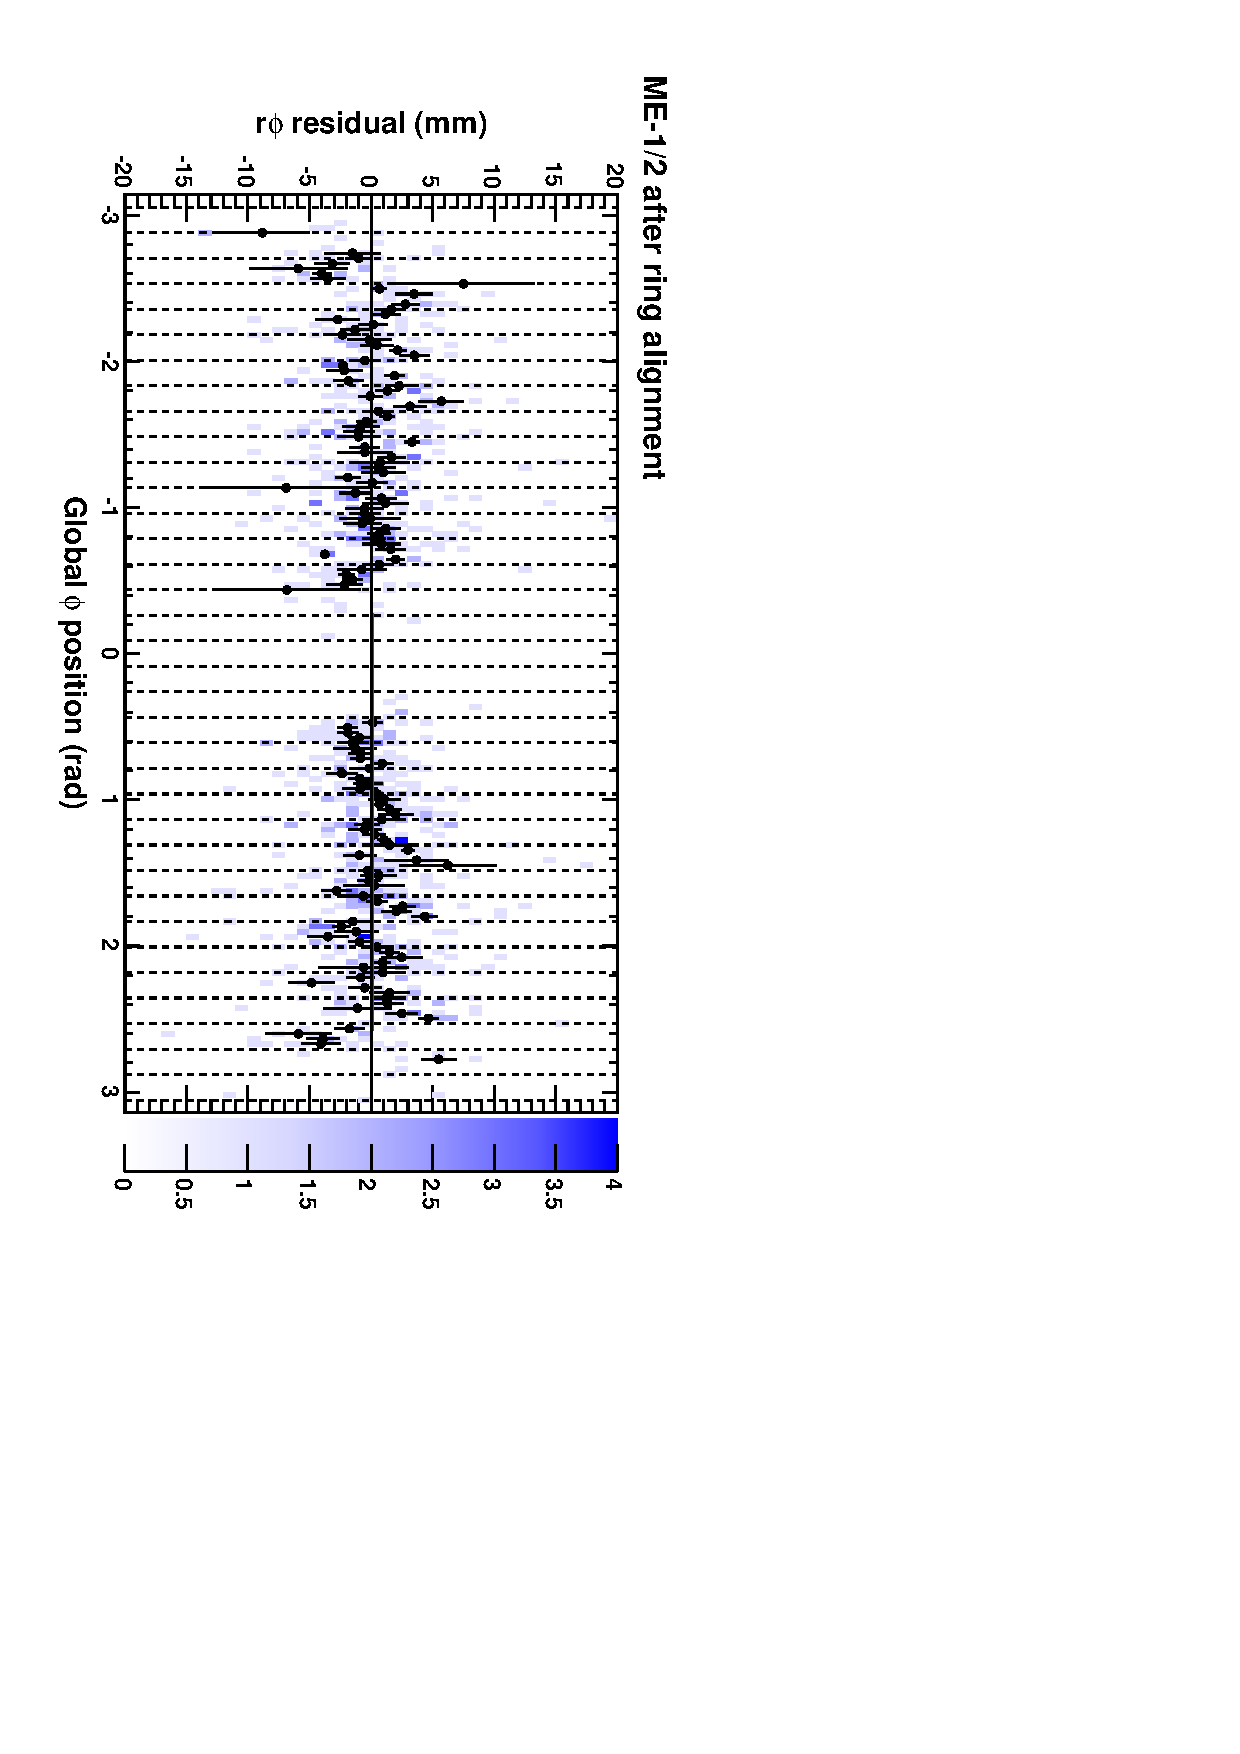
\includegraphics[height=\linewidth, angle=90]{ringfits_after/mem12.pdf}
\column{0.3\linewidth}
\begin{itemize}
\item Color scale is 2-D plot
\item Black points are a profile (averages in vertical bins)
\item Red line is fit to 2-D data
\end{itemize}
\end{columns}
\end{frame}

\begin{frame}
\frametitle{Ring fits: ME$-$1/1}
\vfill
\begin{columns}
\column{0.7\linewidth}
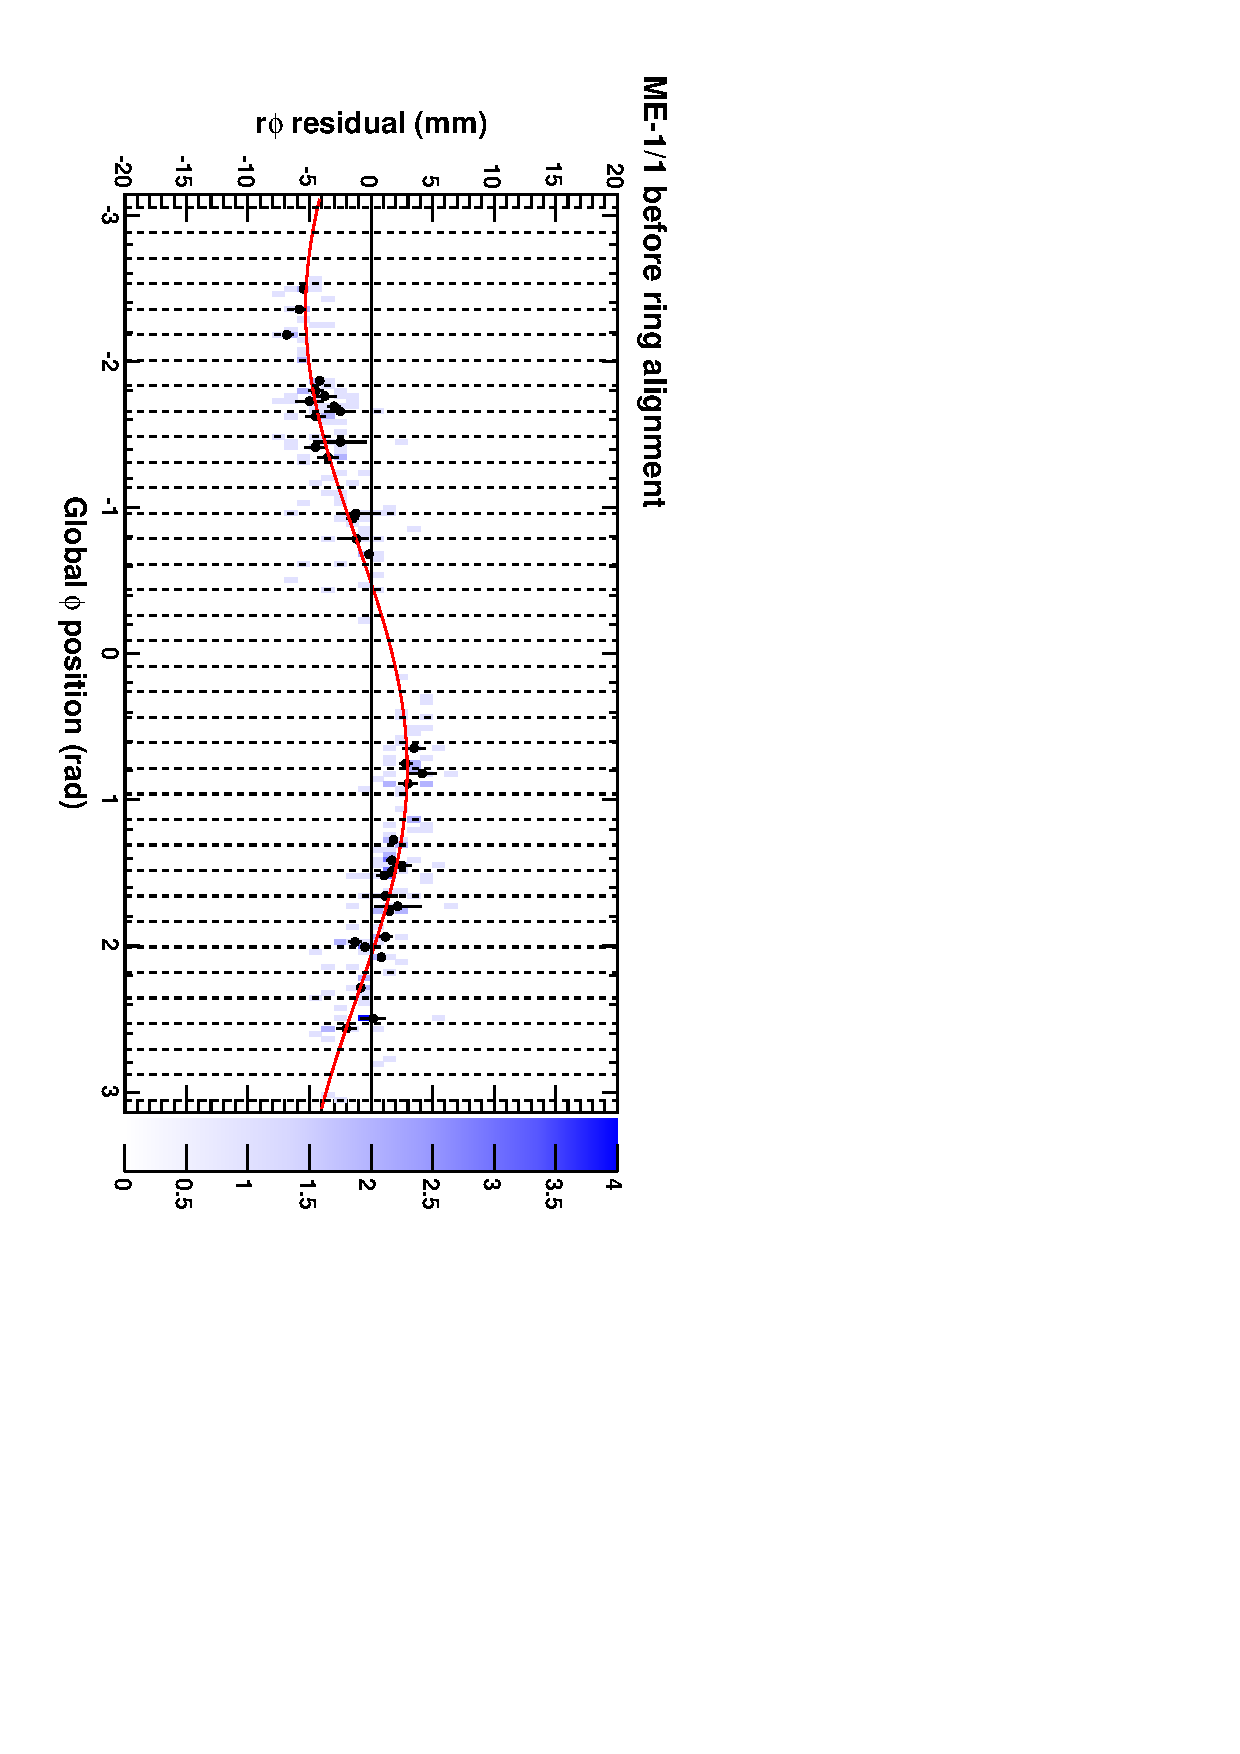
\includegraphics[height=\linewidth, angle=90]{ringfits_before/mem11.pdf}

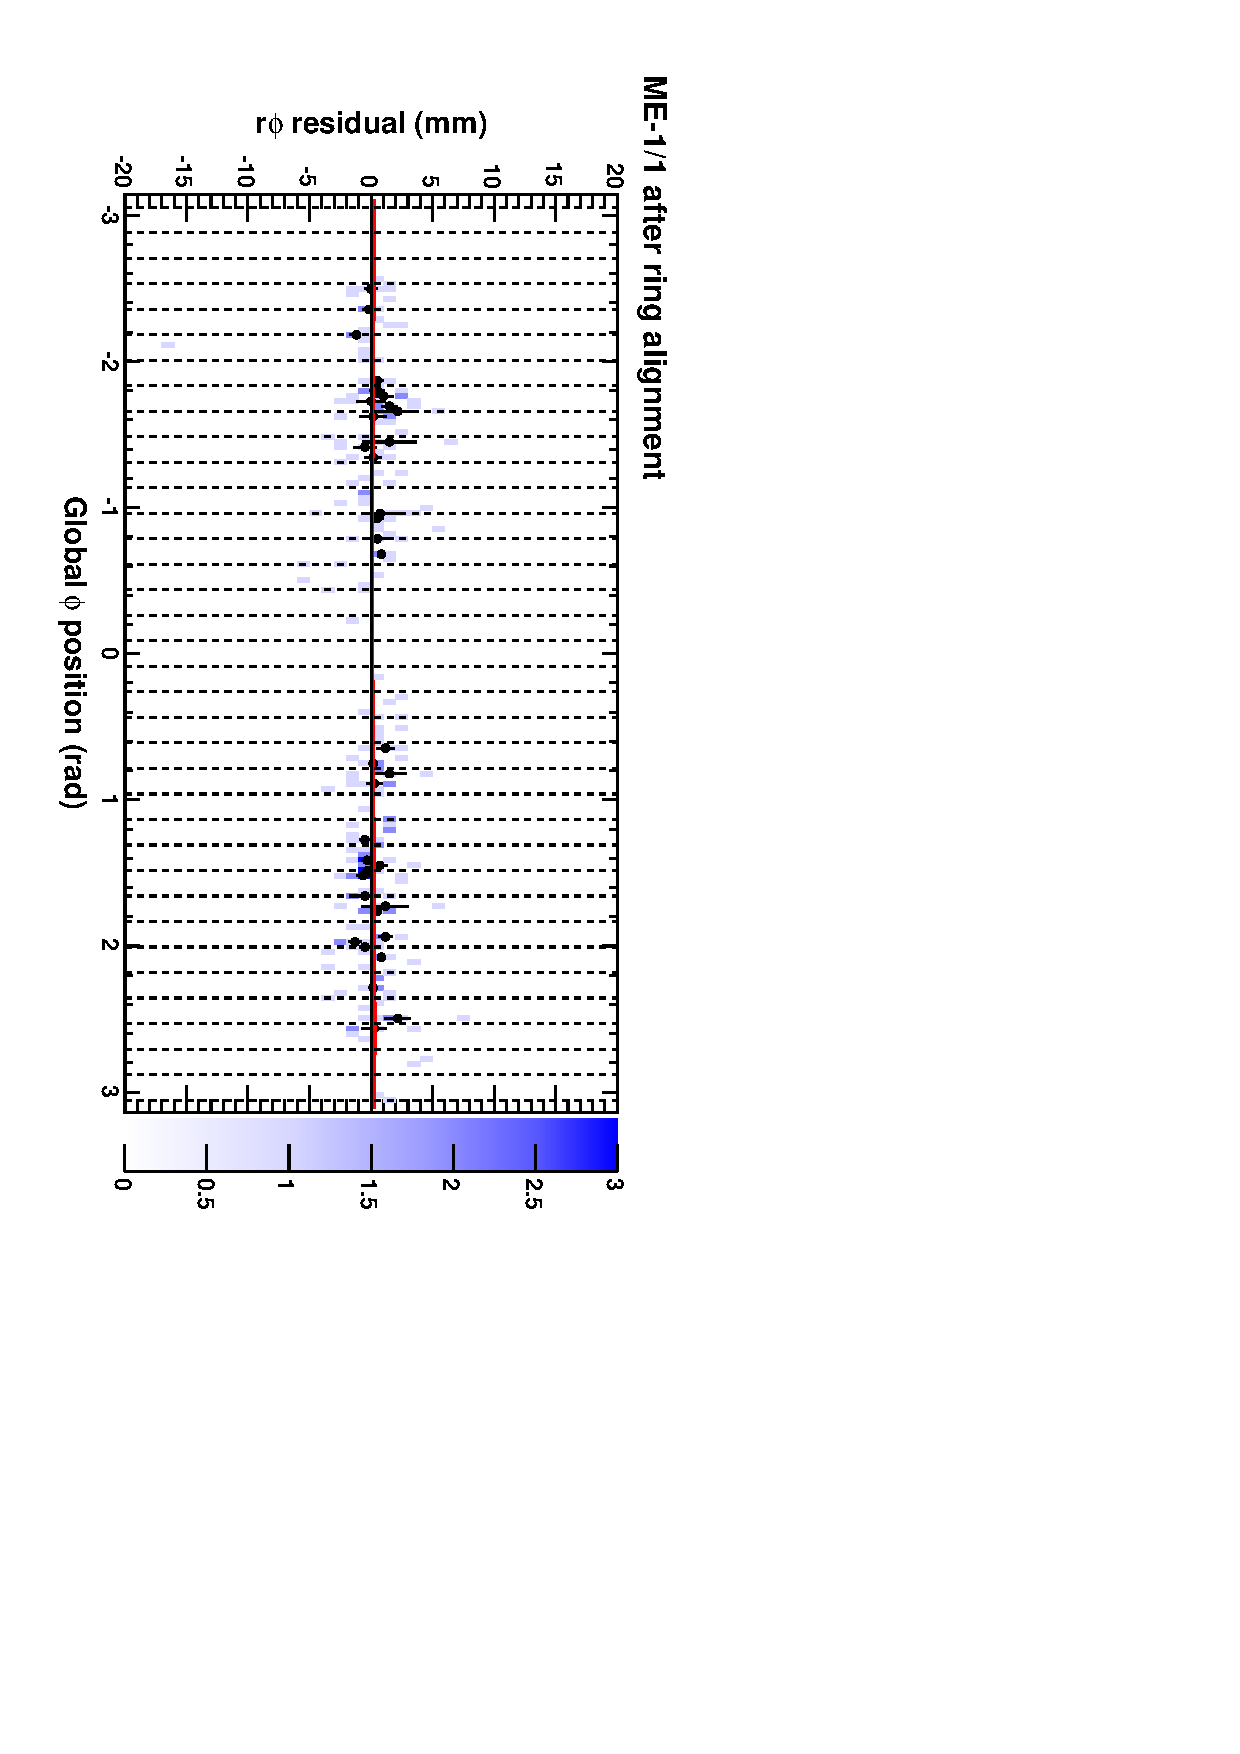
\includegraphics[height=\linewidth, angle=90]{ringfits_after/mem11.pdf}
\column{0.3\linewidth}
\begin{itemize}
\item Color scale is 2-D plot
\item Black points are a profile (averages in vertical bins)
\item Red line is fit to 2-D data
\end{itemize}
\end{columns}
\end{frame}

\begin{frame}
\frametitle{Ring fits: ME$+$1/1}
\vfill
\begin{columns}
\column{0.7\linewidth}
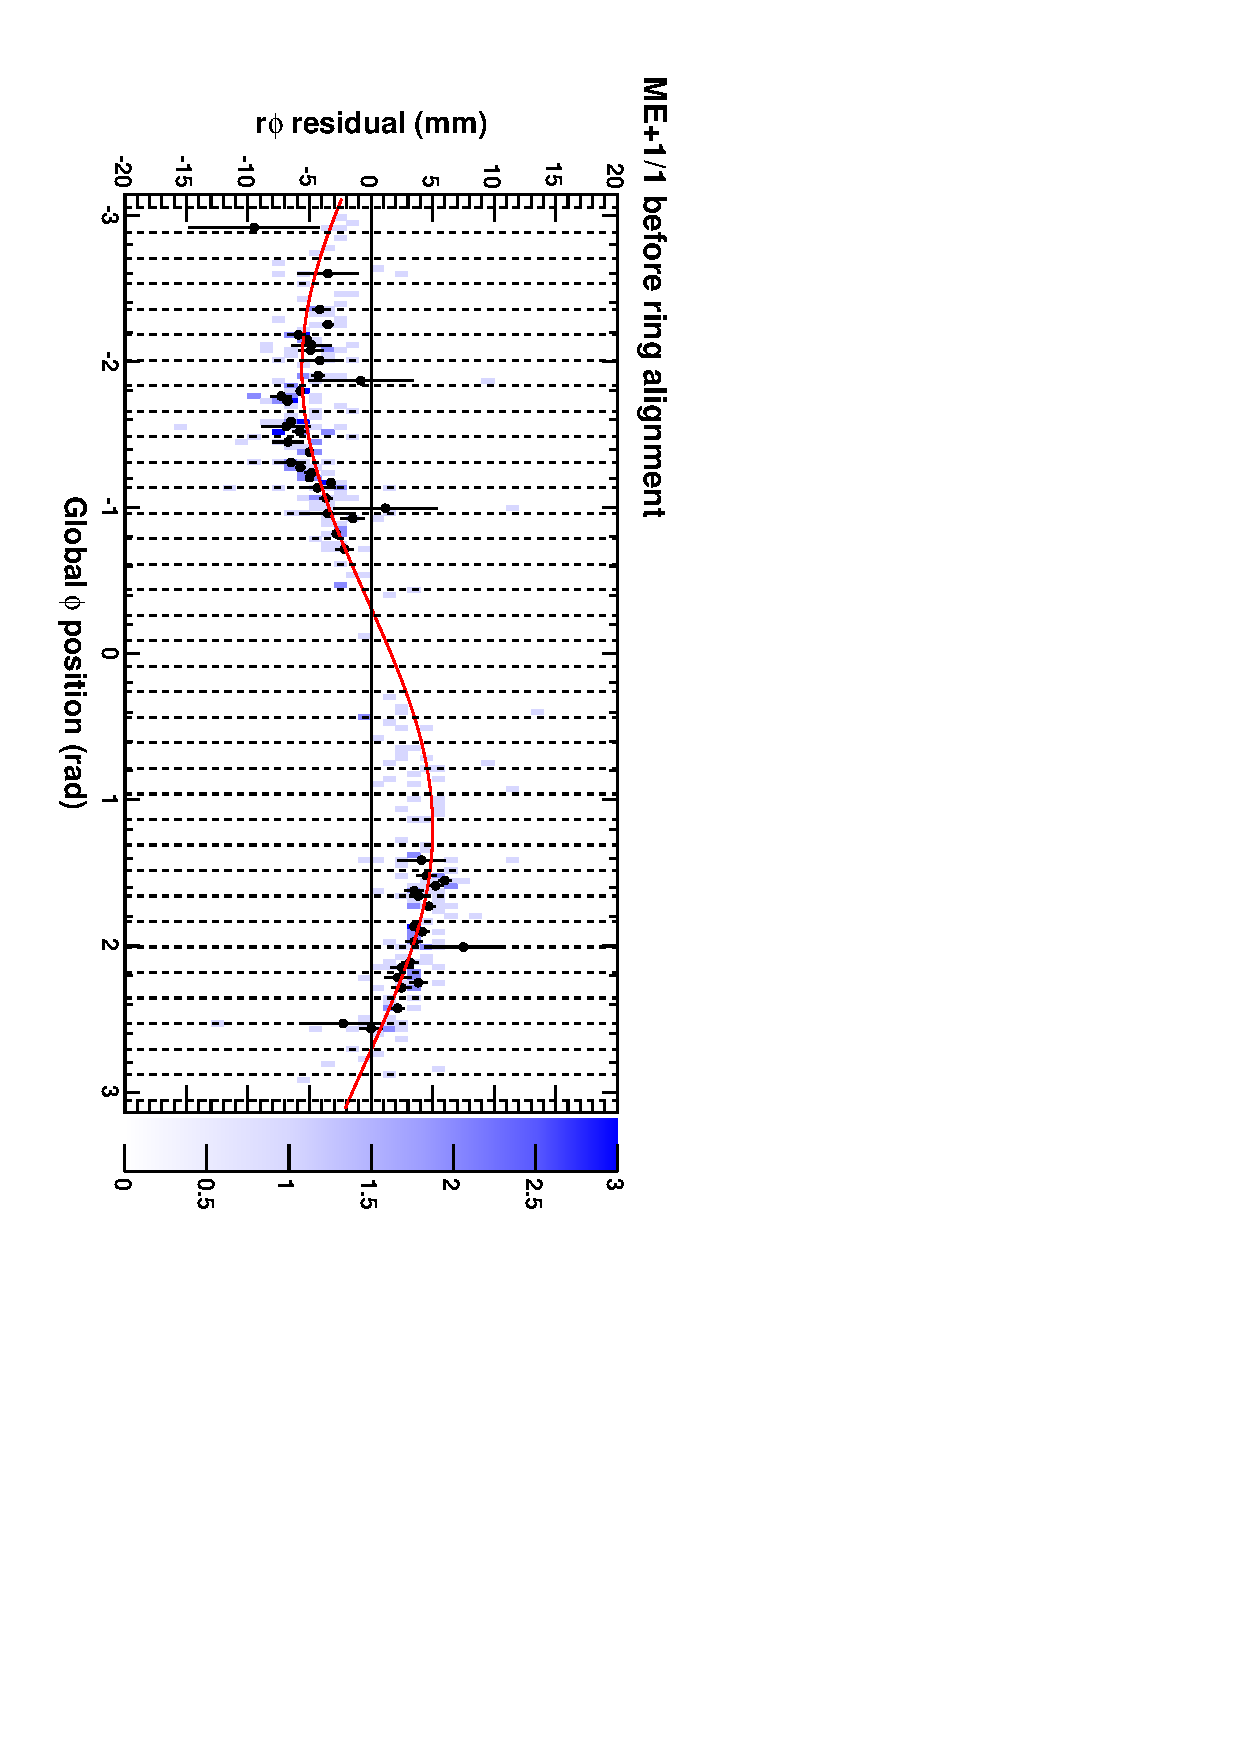
\includegraphics[height=\linewidth, angle=90]{ringfits_before/mep11.pdf}

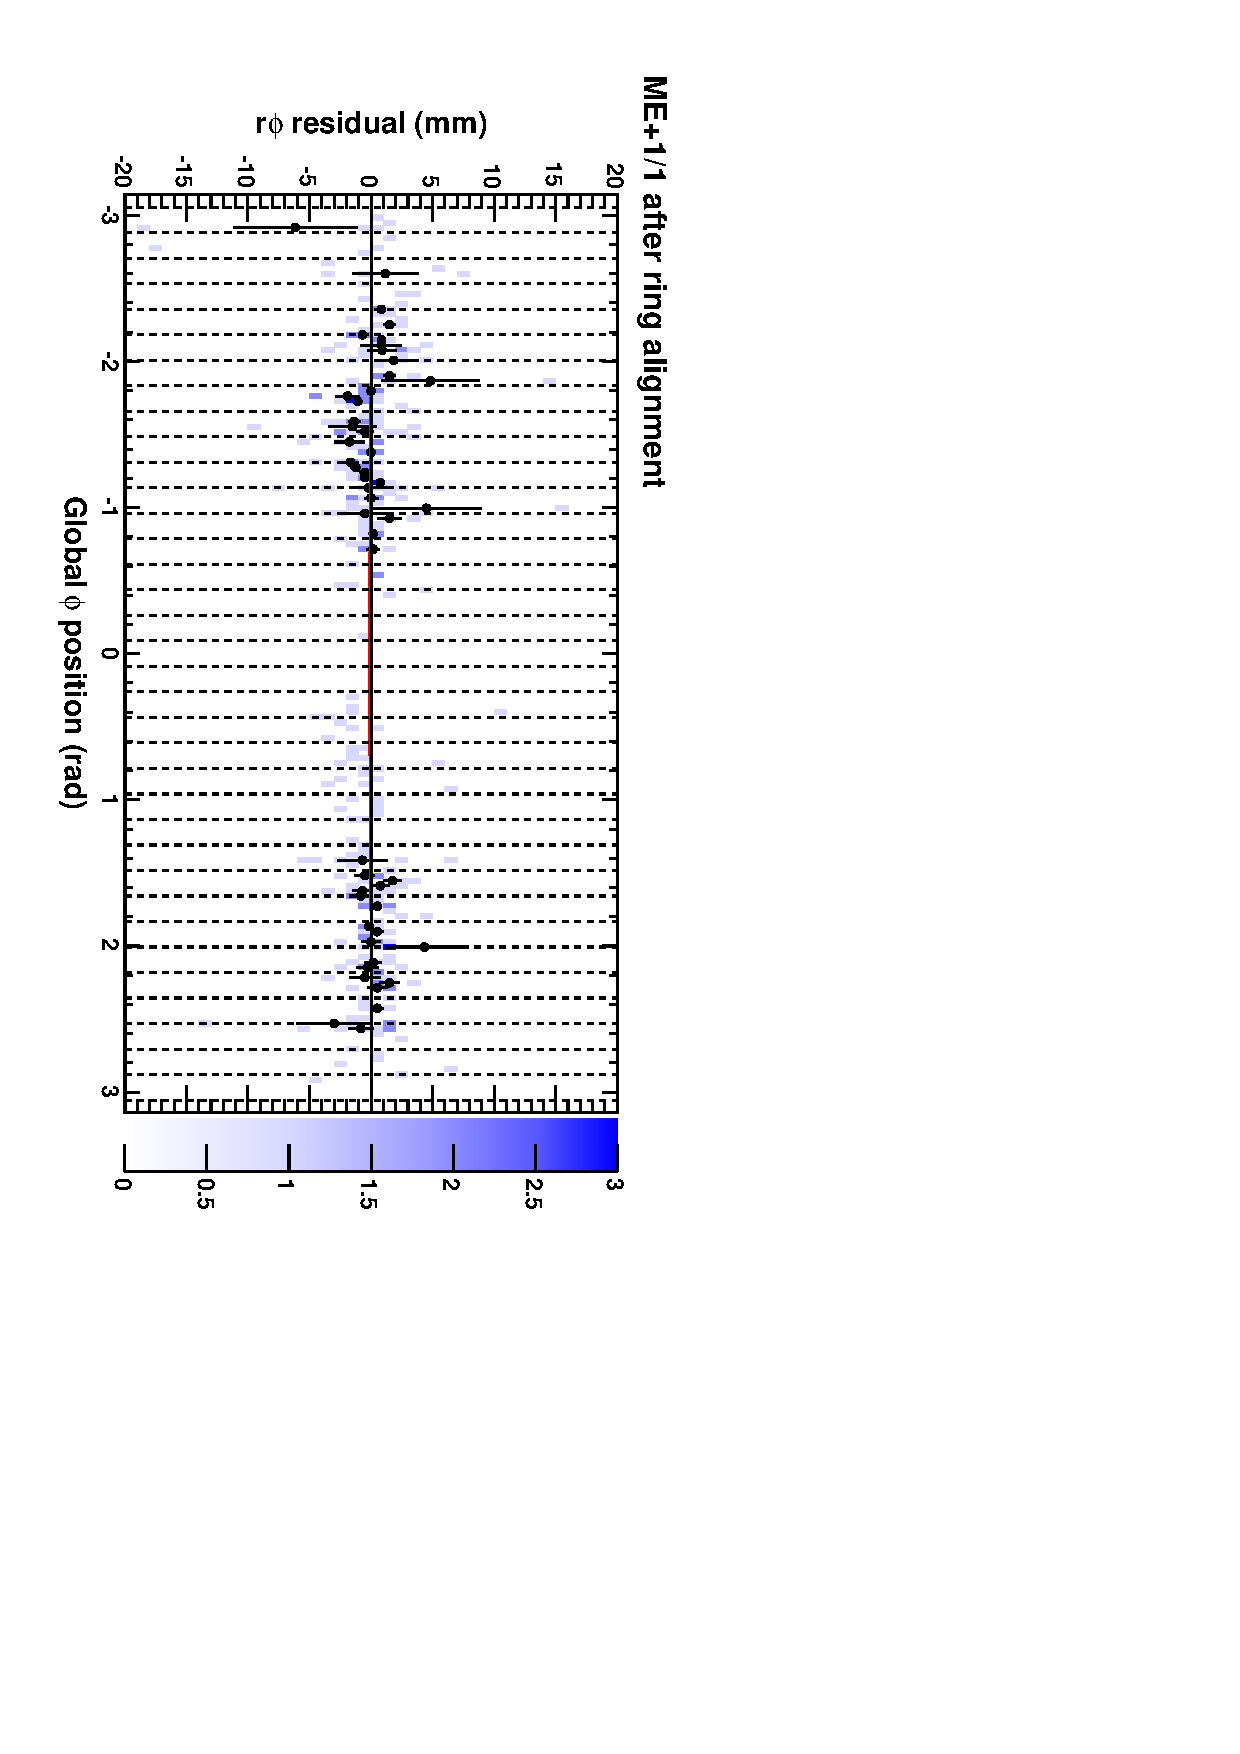
\includegraphics[height=\linewidth, angle=90]{ringfits_after/mep11.pdf}
\column{0.3\linewidth}
\begin{itemize}
\item Color scale is 2-D plot
\item Black points are a profile (averages in vertical bins)
\item Red line is fit to 2-D data
\end{itemize}
\end{columns}
\end{frame}

\begin{frame}
\frametitle{Ring fits: ME$+$1/2}
\vfill
\begin{columns}
\column{0.7\linewidth}
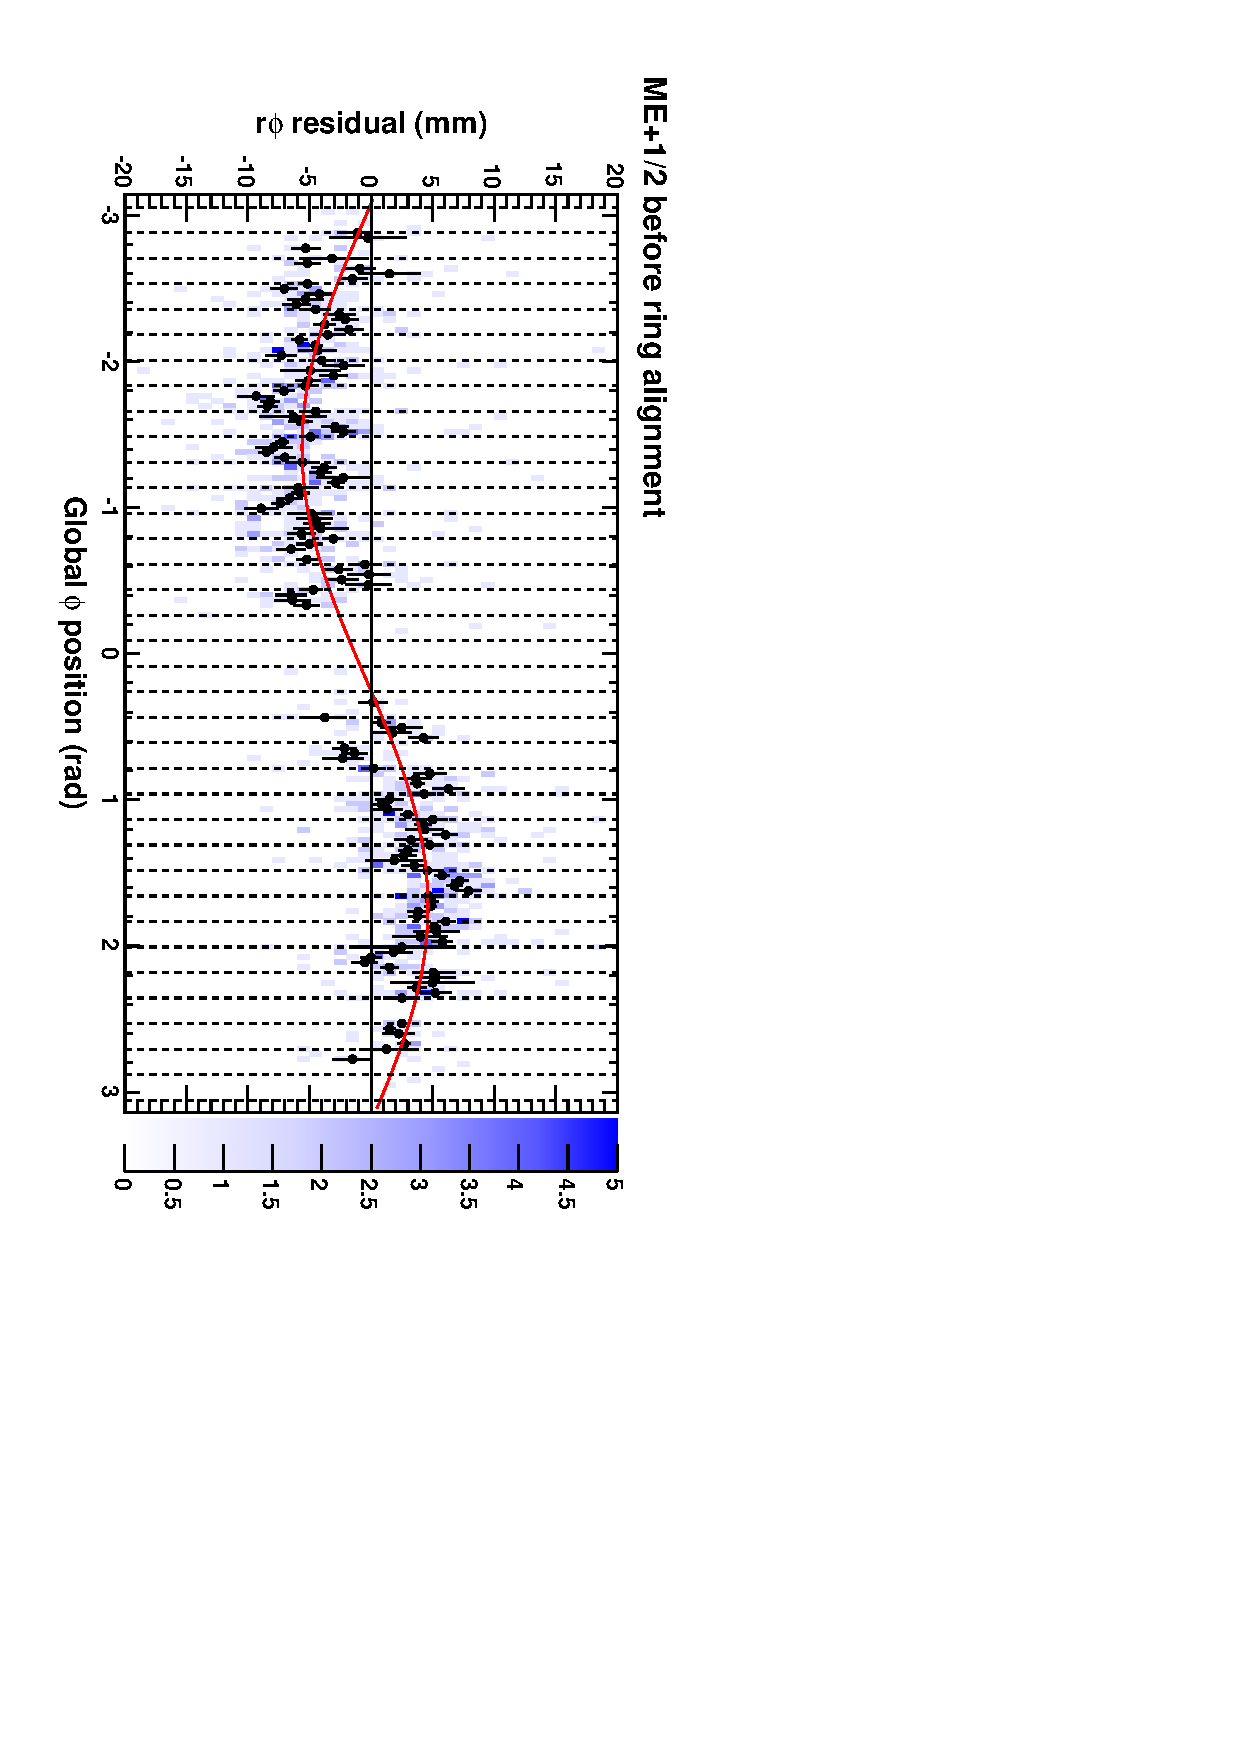
\includegraphics[height=\linewidth, angle=90]{ringfits_before/mep12.pdf}

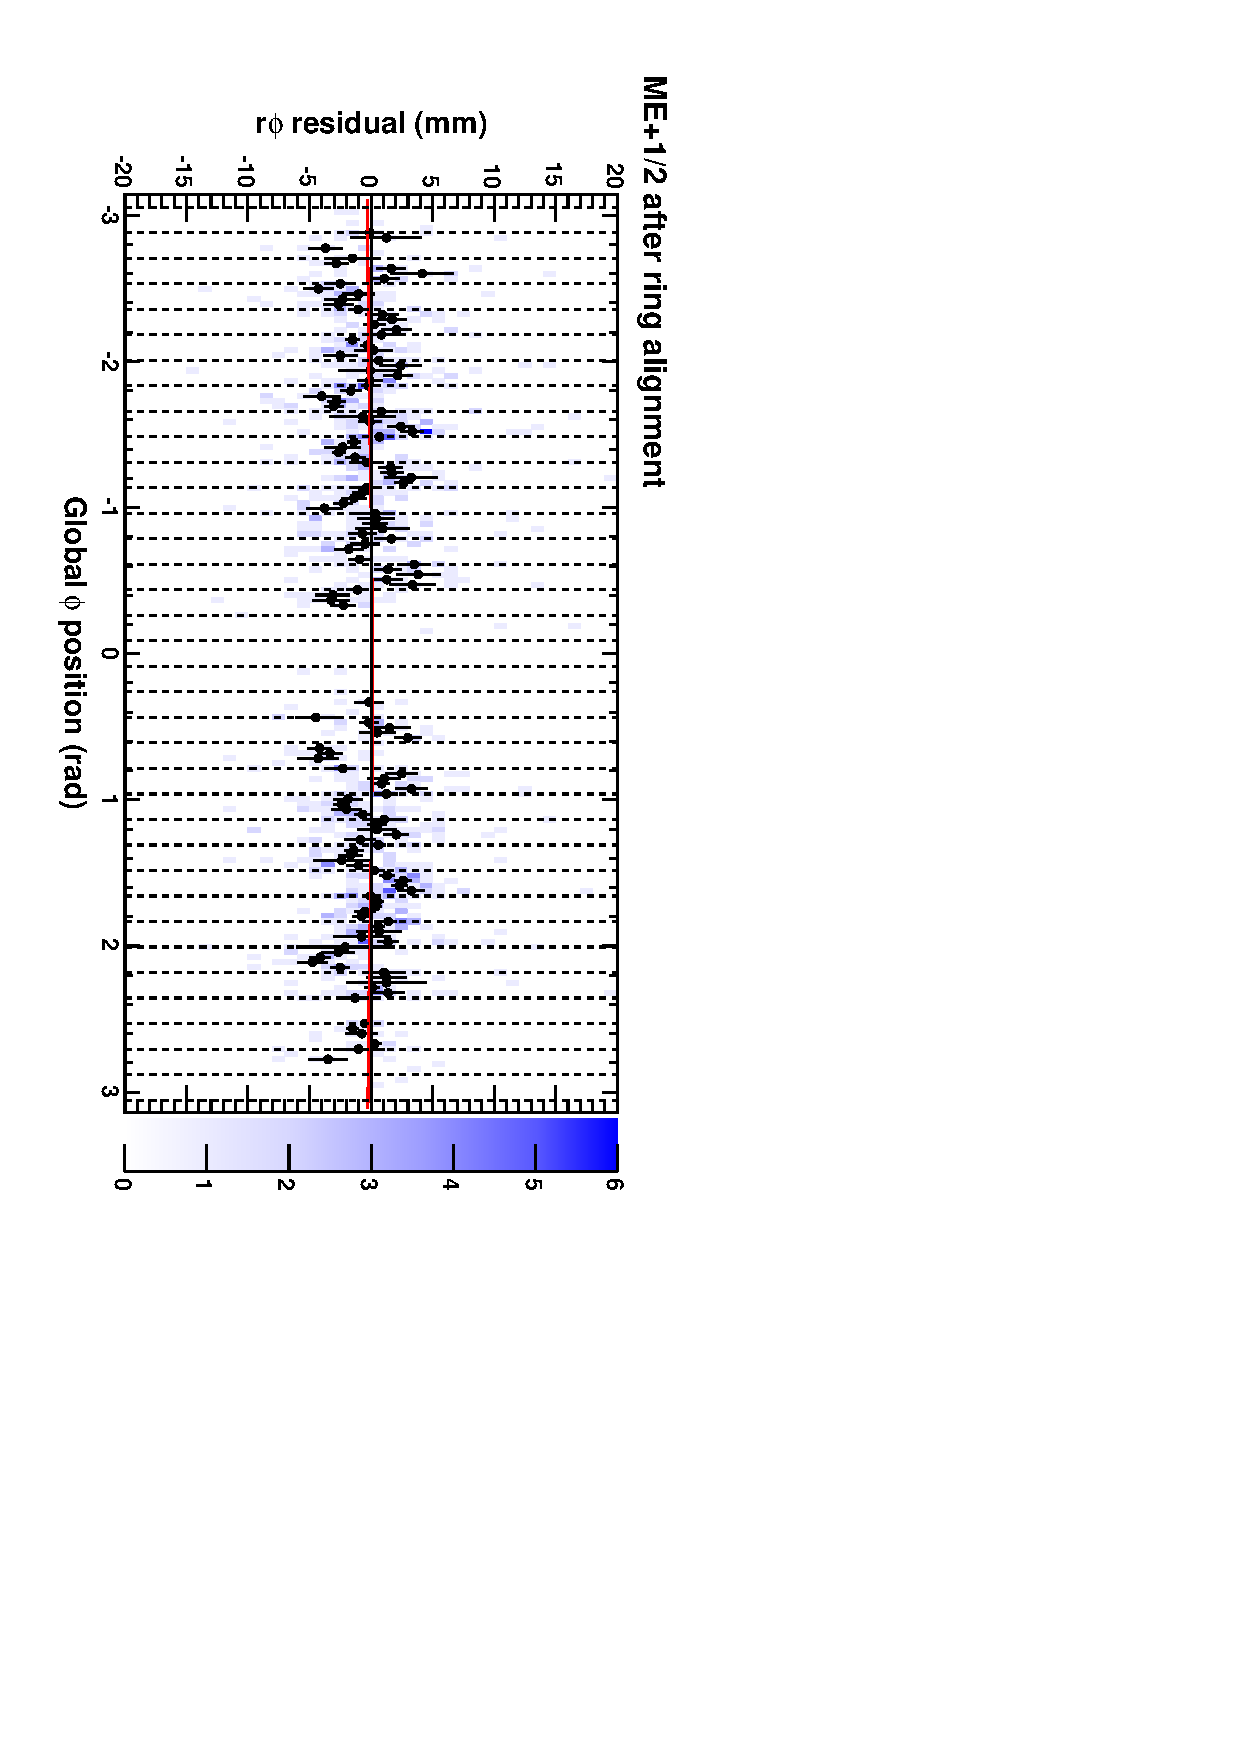
\includegraphics[height=\linewidth, angle=90]{ringfits_after/mep12.pdf}
\column{0.3\linewidth}
\begin{itemize}
\item Color scale is 2-D plot
\item Black points are a profile (averages in vertical bins)
\item Red line is fit to 2-D data
\end{itemize}
\end{columns}
\end{frame}

\begin{frame}
\frametitle{Ring fits: ME$+$1/3}
\vfill
\begin{columns}
\column{0.7\linewidth}
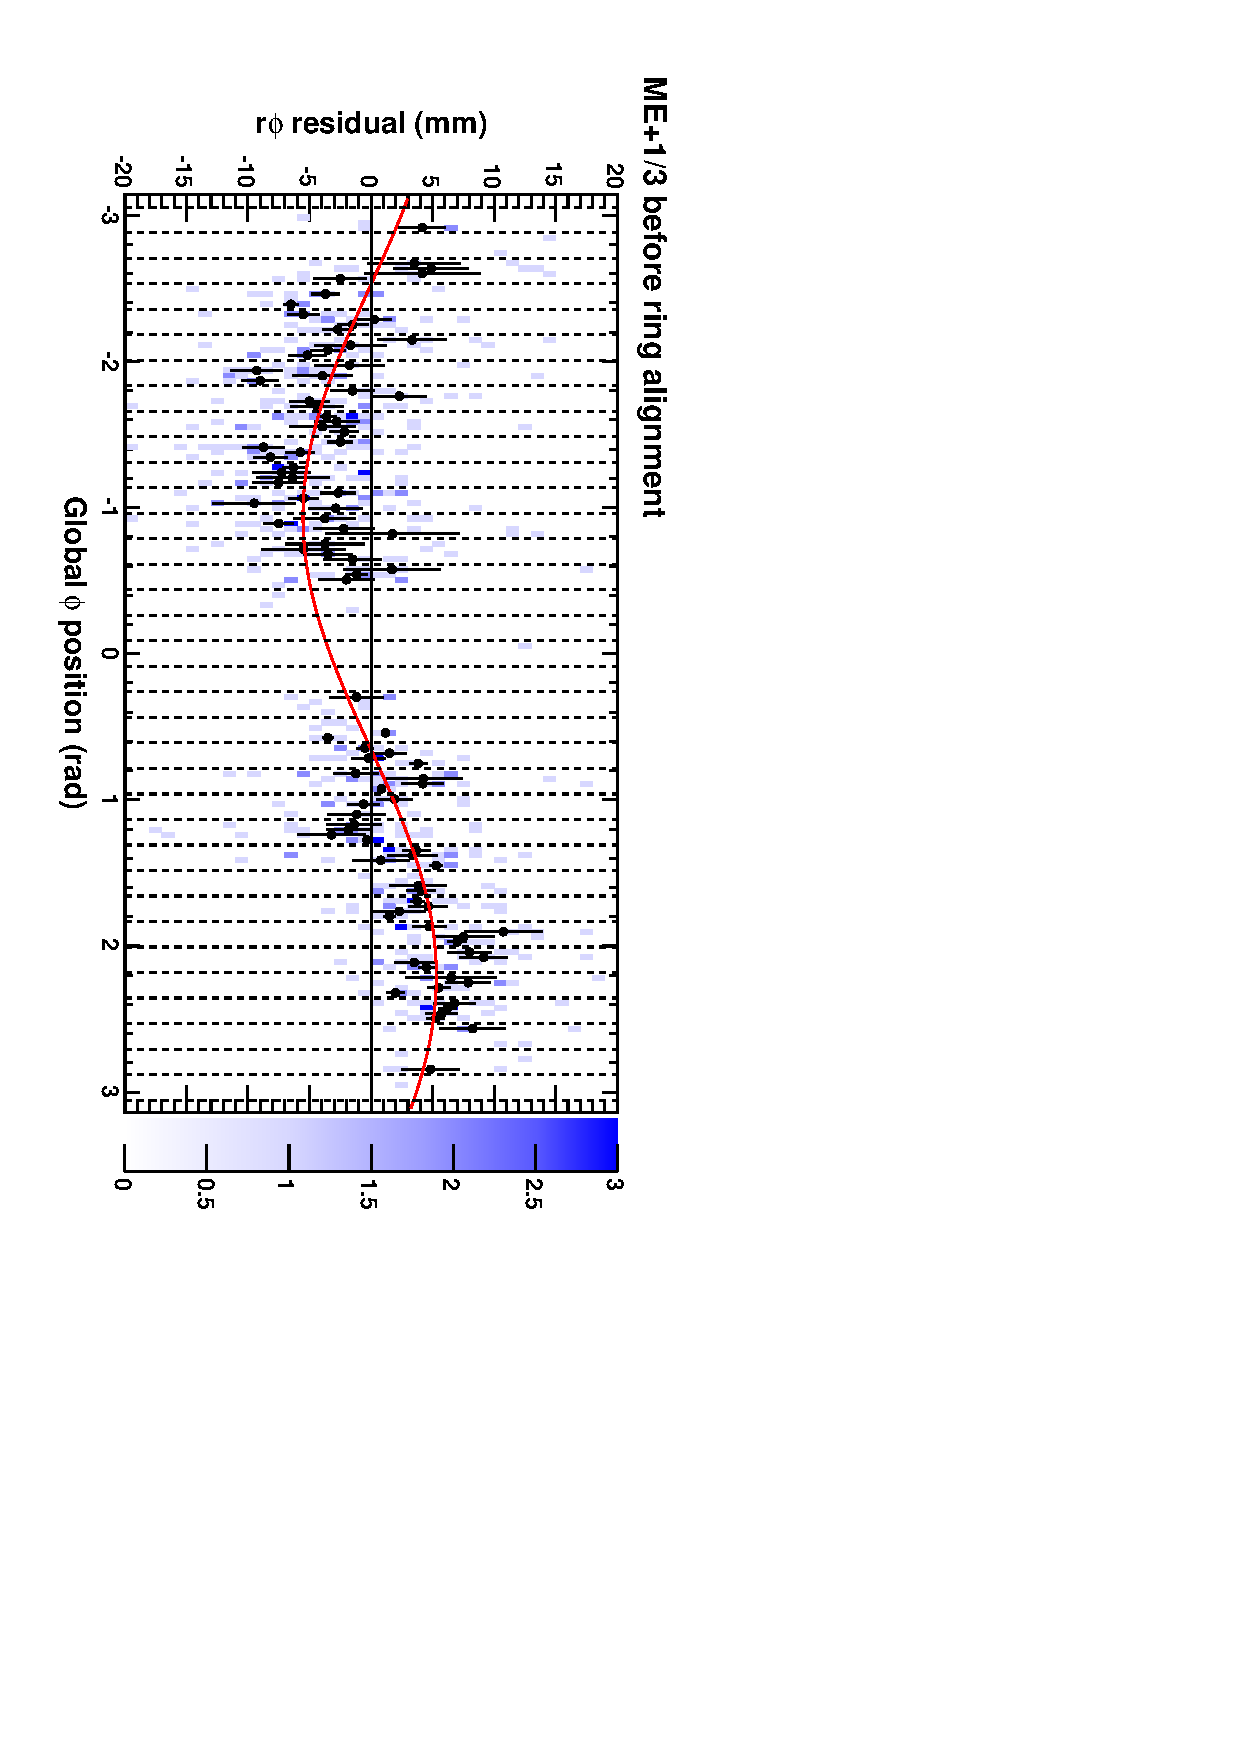
\includegraphics[height=\linewidth, angle=90]{ringfits_before/mep13.pdf}

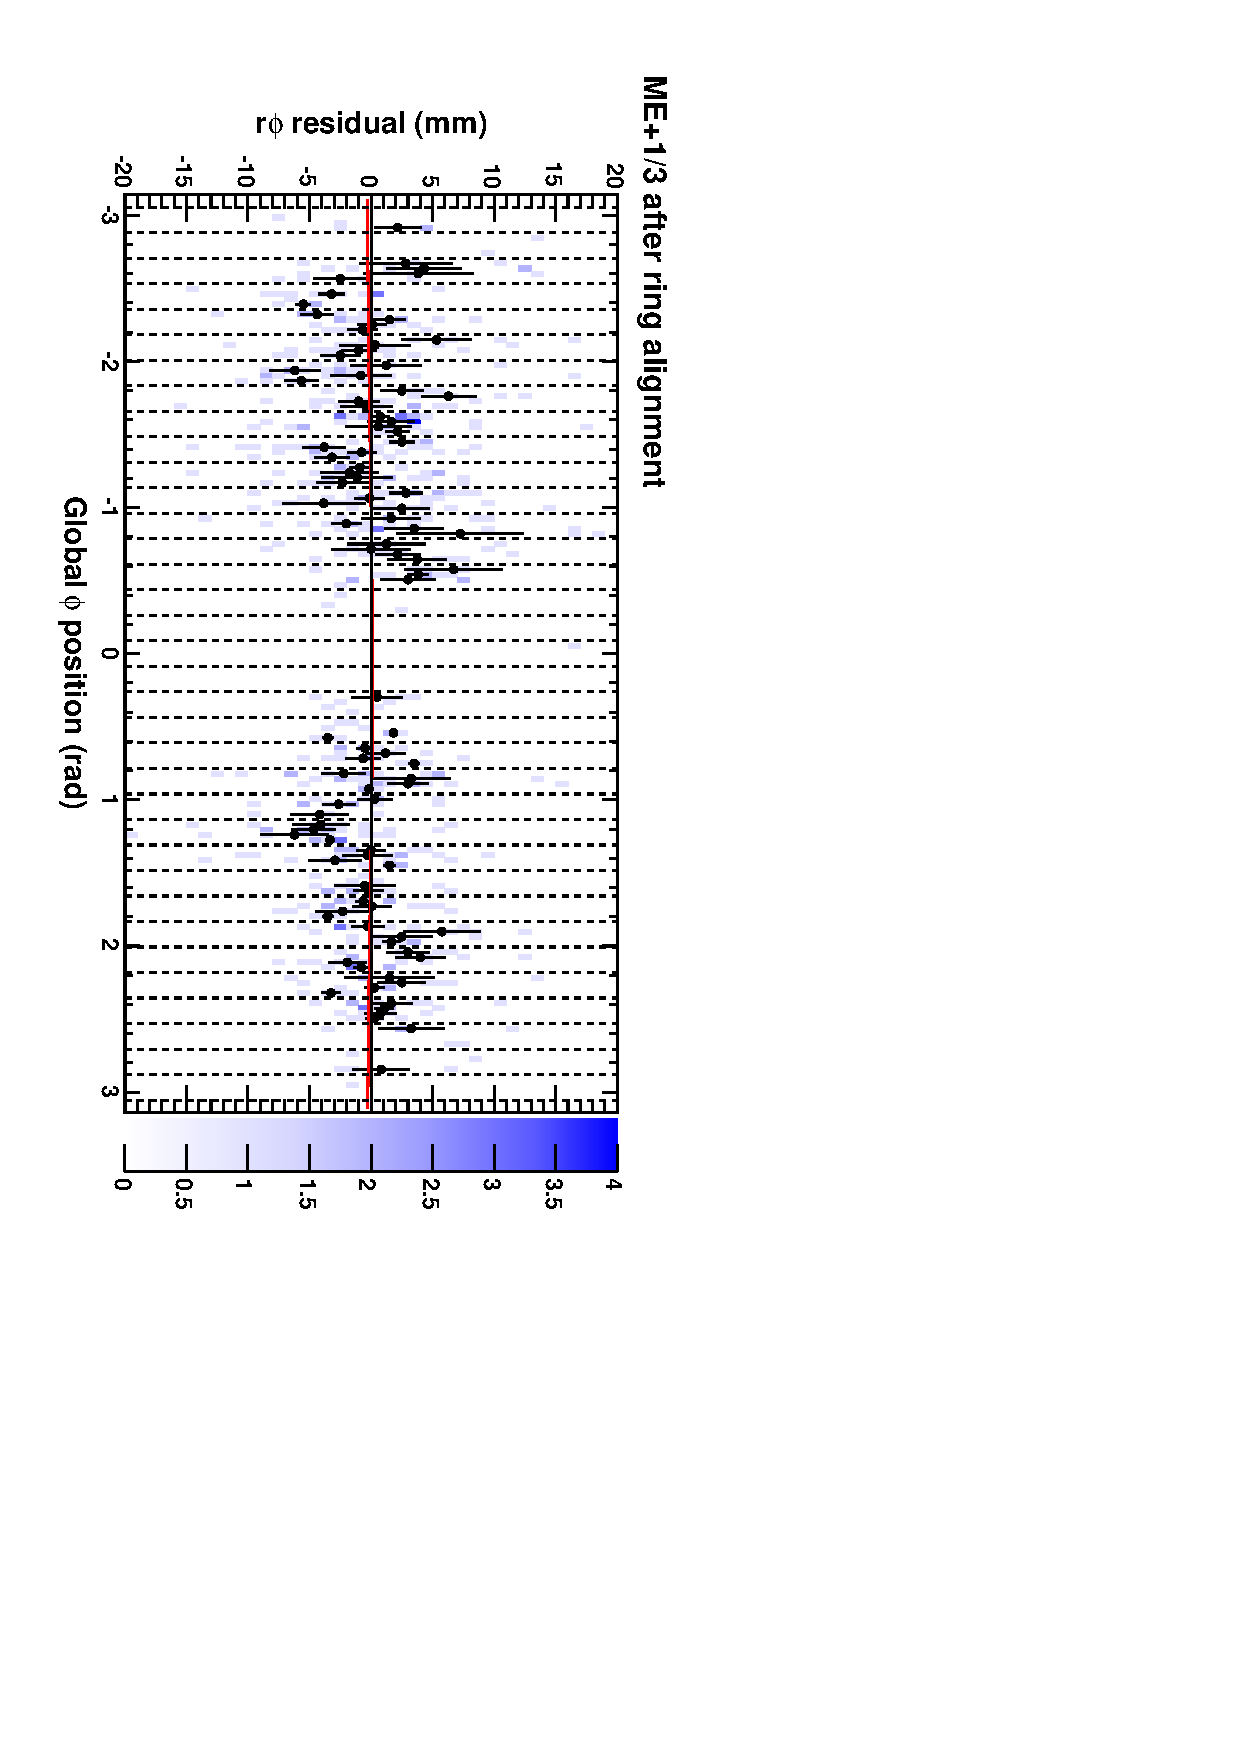
\includegraphics[height=\linewidth, angle=90]{ringfits_after/mep13.pdf}
\column{0.3\linewidth}
\begin{itemize}
\item Color scale is 2-D plot
\item Black points are a profile (averages in vertical bins)
\item Red line is fit to 2-D data
\end{itemize}
\end{columns}
\end{frame}

\begin{frame}
\frametitle{Ring fits: ME$+$2/1}
\vfill
\begin{columns}
\column{0.7\linewidth}
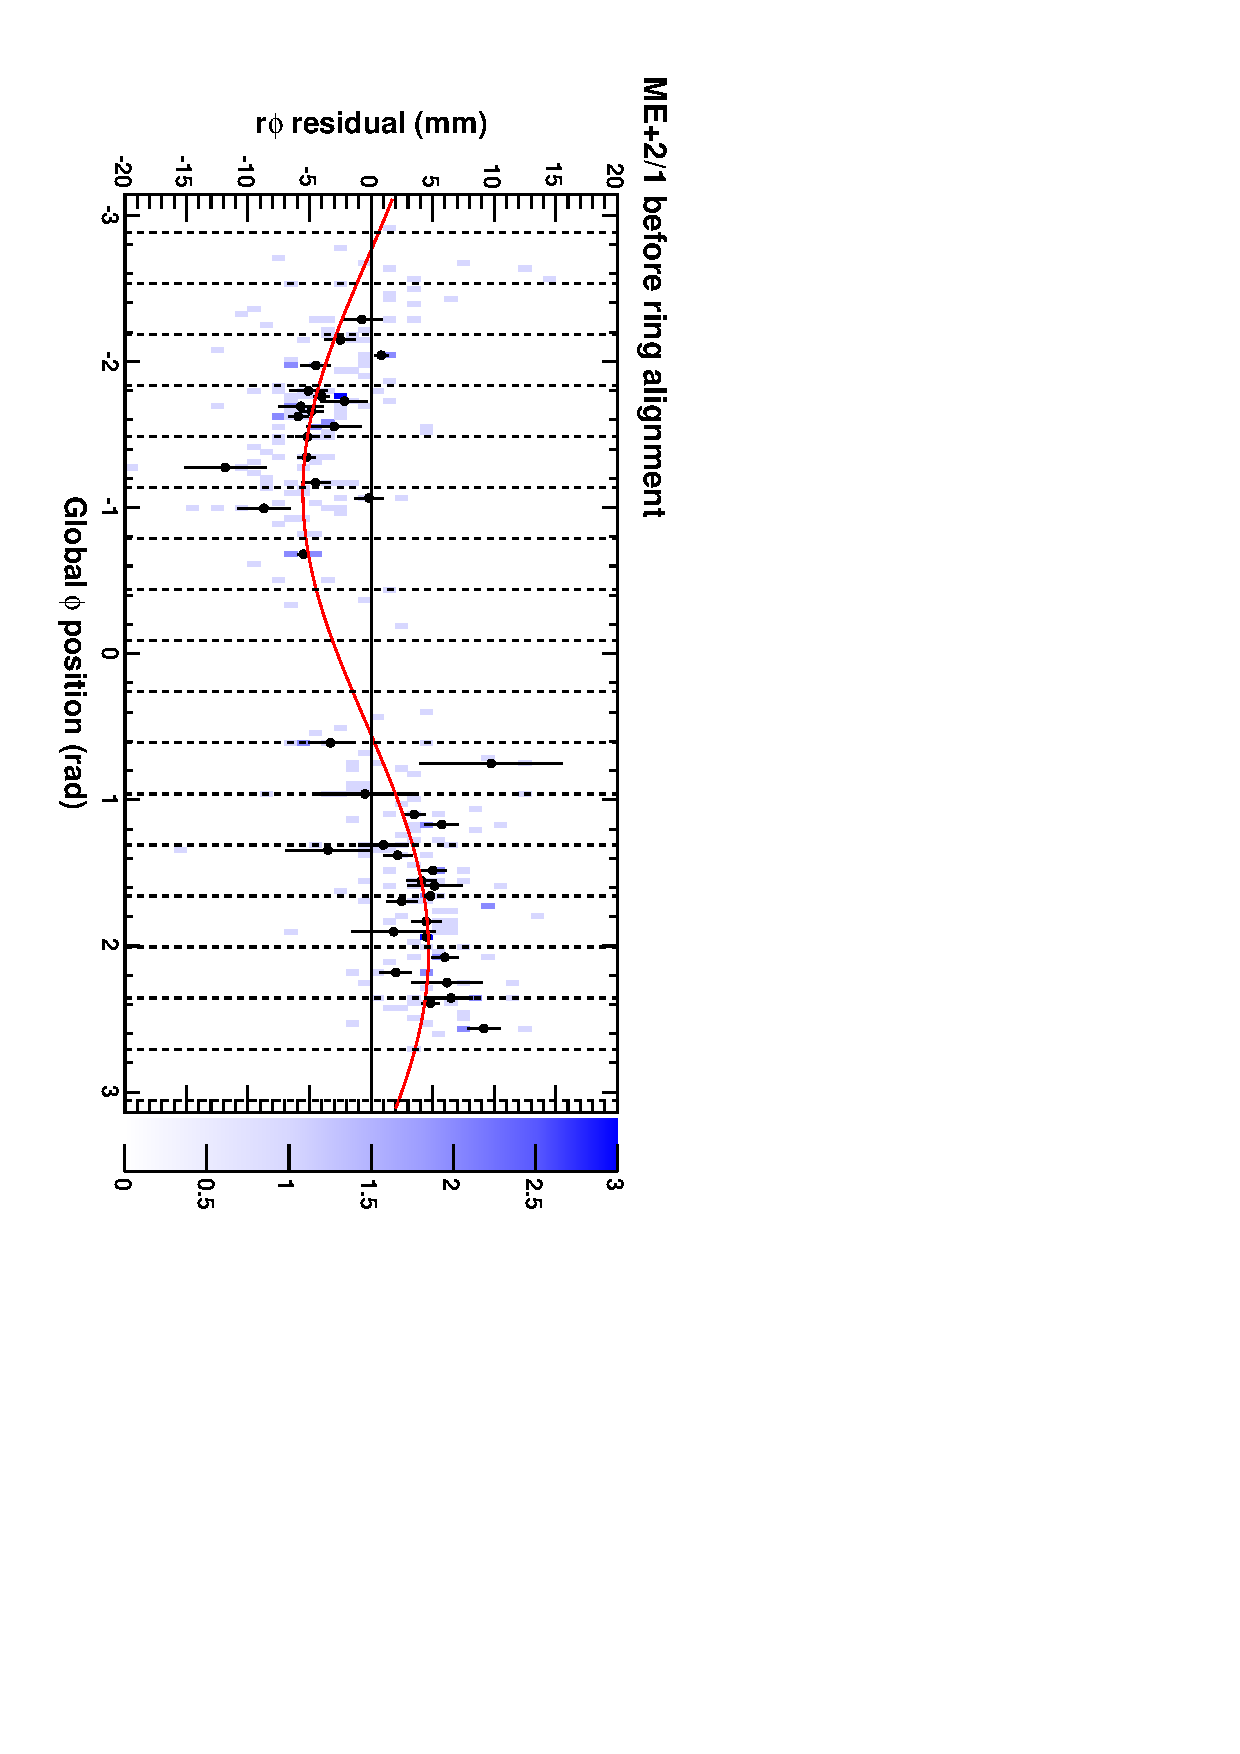
\includegraphics[height=\linewidth, angle=90]{ringfits_before/mep21.pdf}

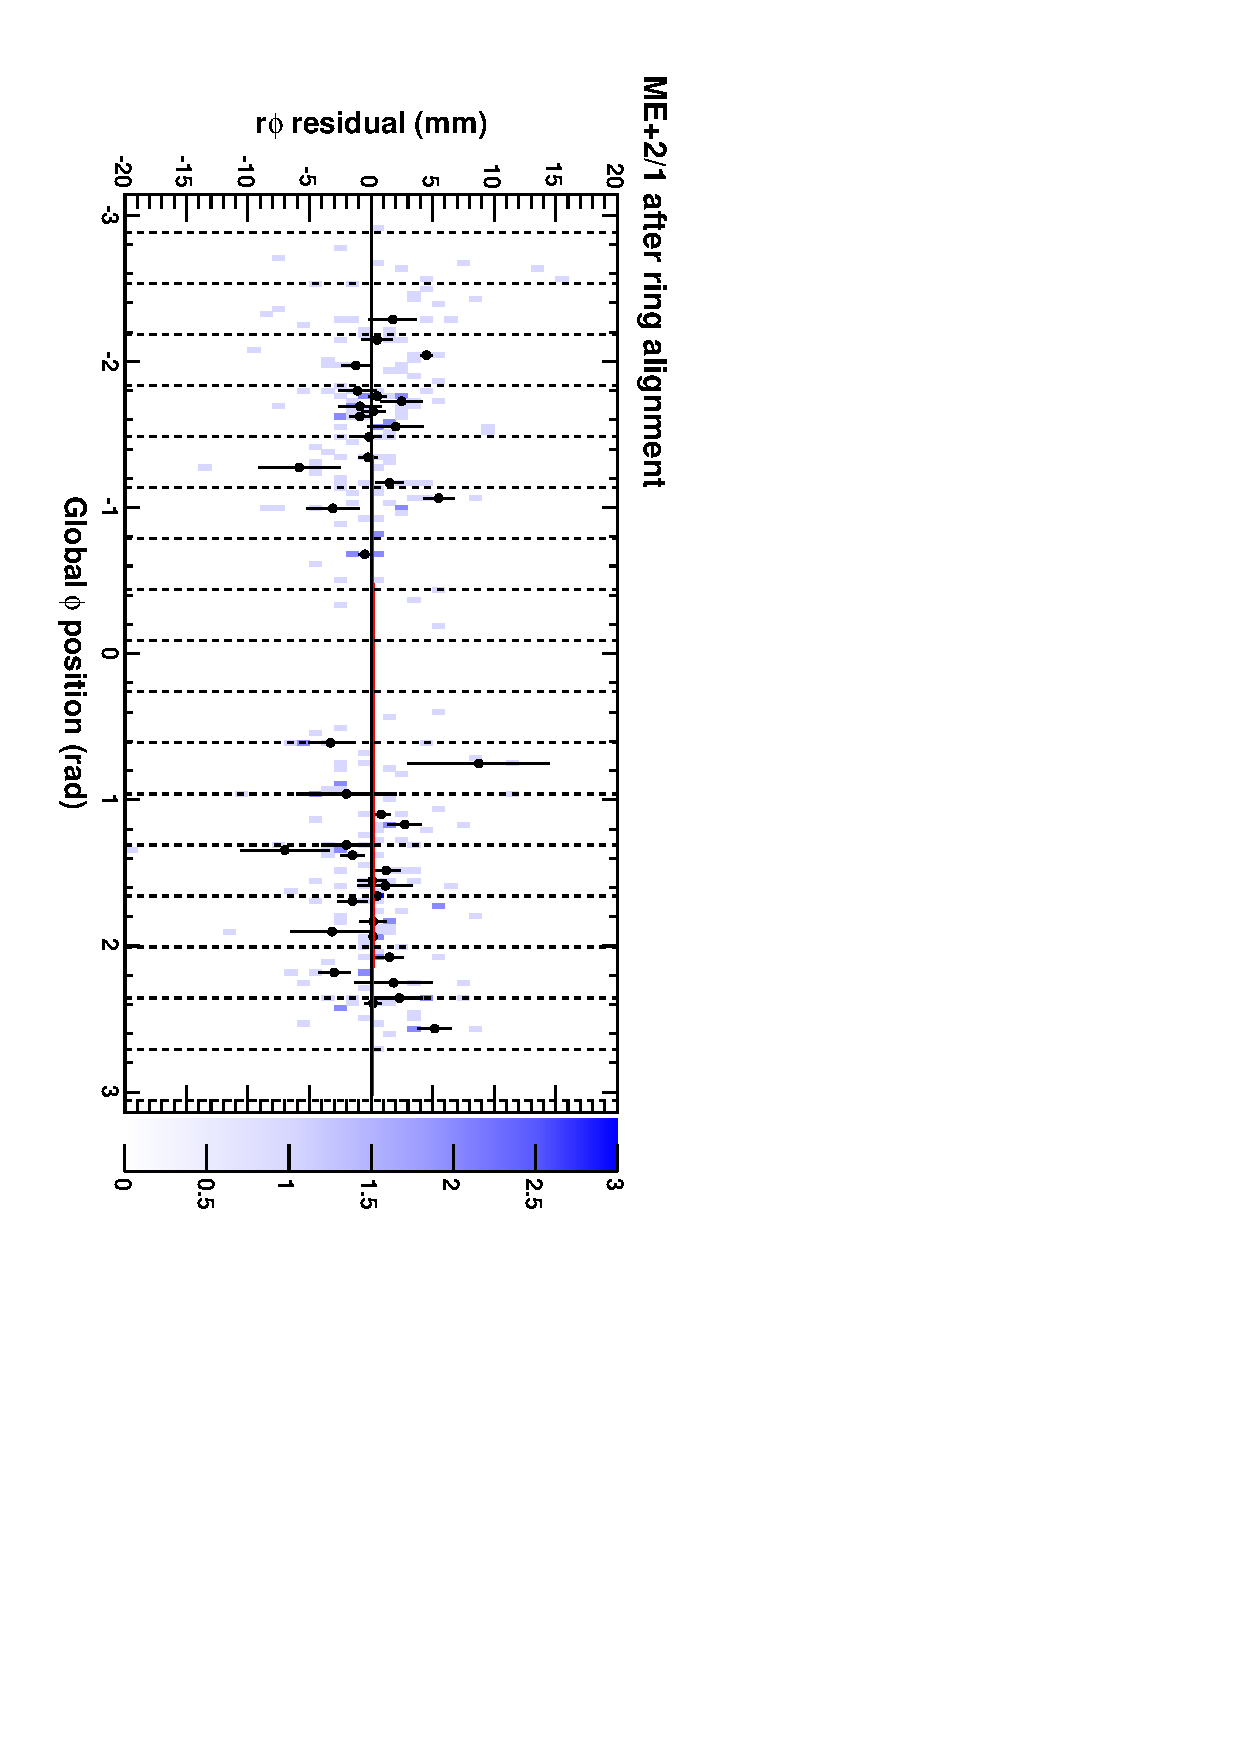
\includegraphics[height=\linewidth, angle=90]{ringfits_after/mep21.pdf}
\column{0.3\linewidth}
\begin{itemize}
\item Color scale is 2-D plot
\item Black points are a profile (averages in vertical bins)
\item Red line is fit to 2-D data
\end{itemize}
\end{columns}
\end{frame}

\begin{frame}
\frametitle{Ring fits: ME$+$2/2}
\vfill
\begin{columns}
\column{0.7\linewidth}
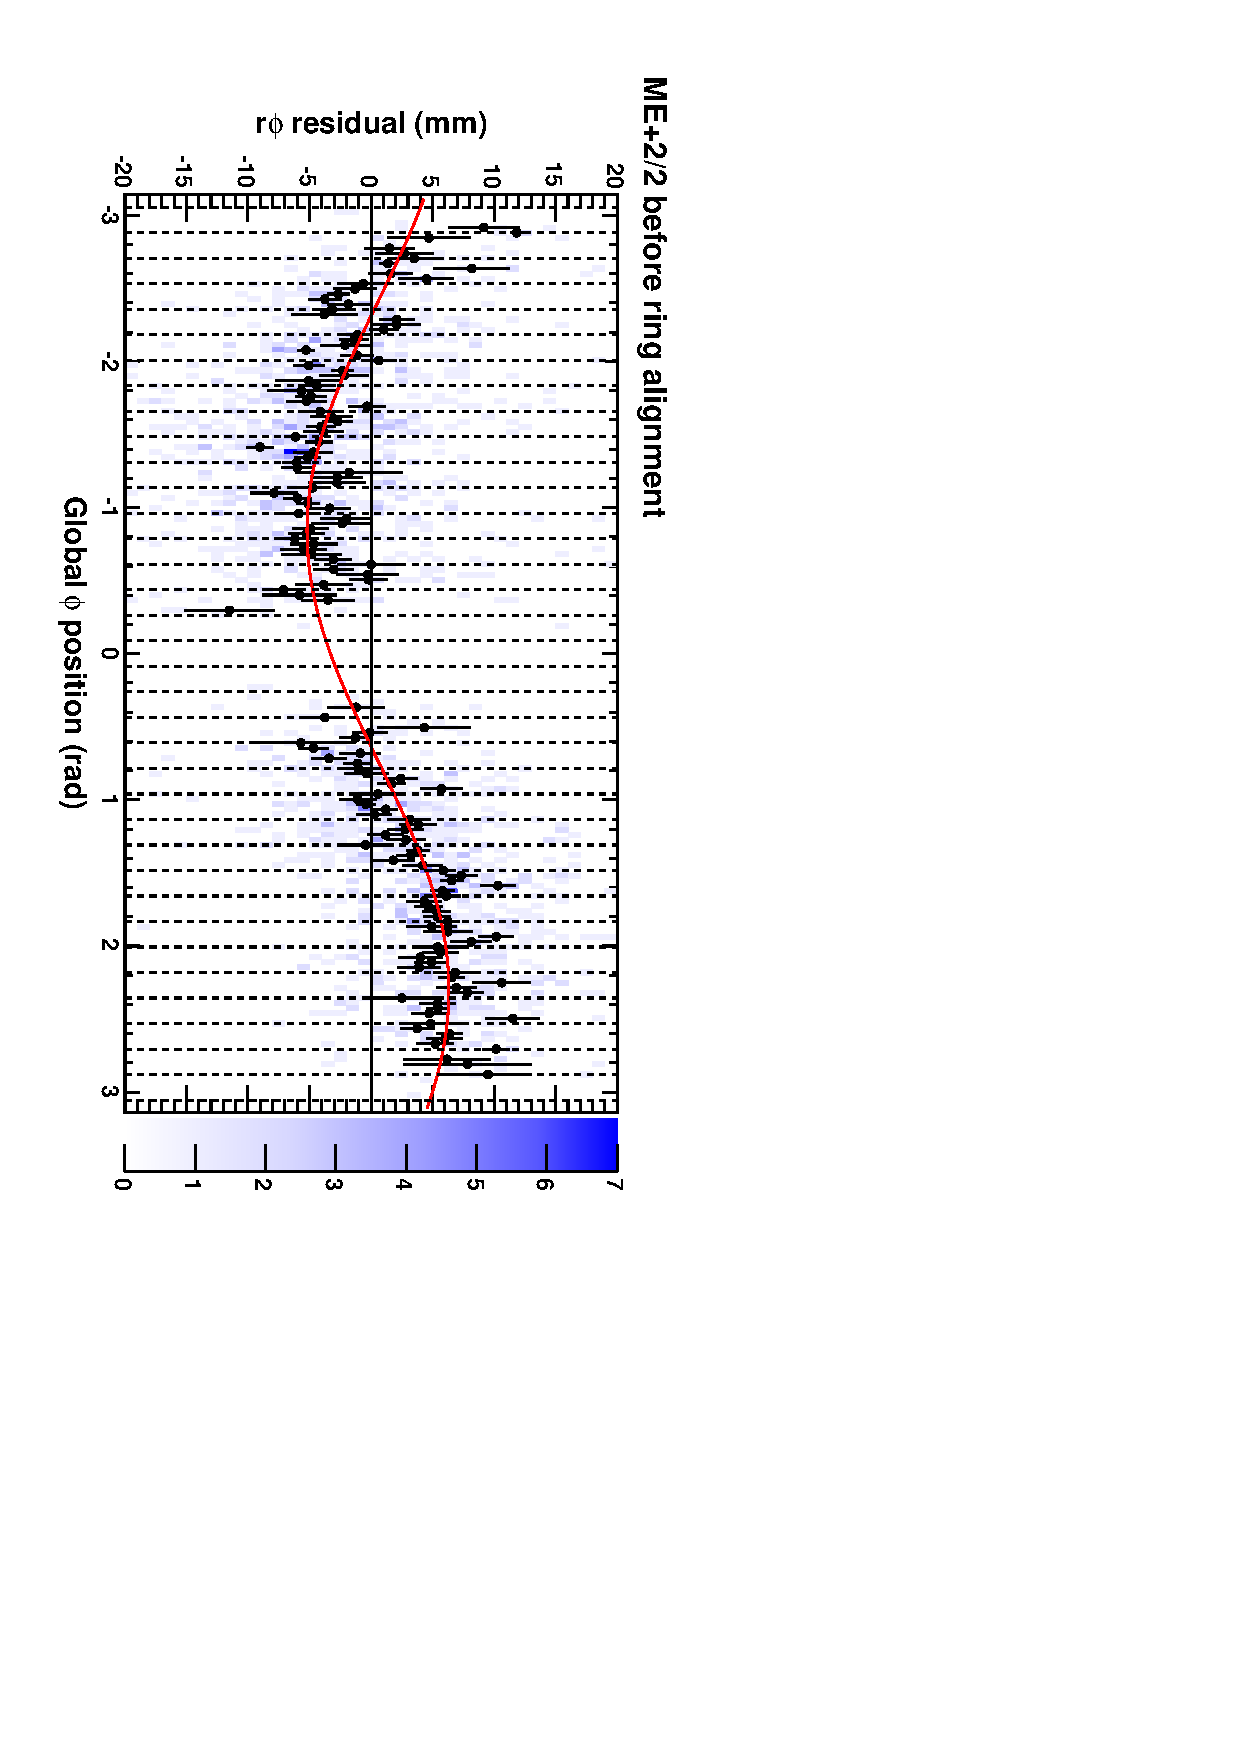
\includegraphics[height=\linewidth, angle=90]{ringfits_before/mep22.pdf}

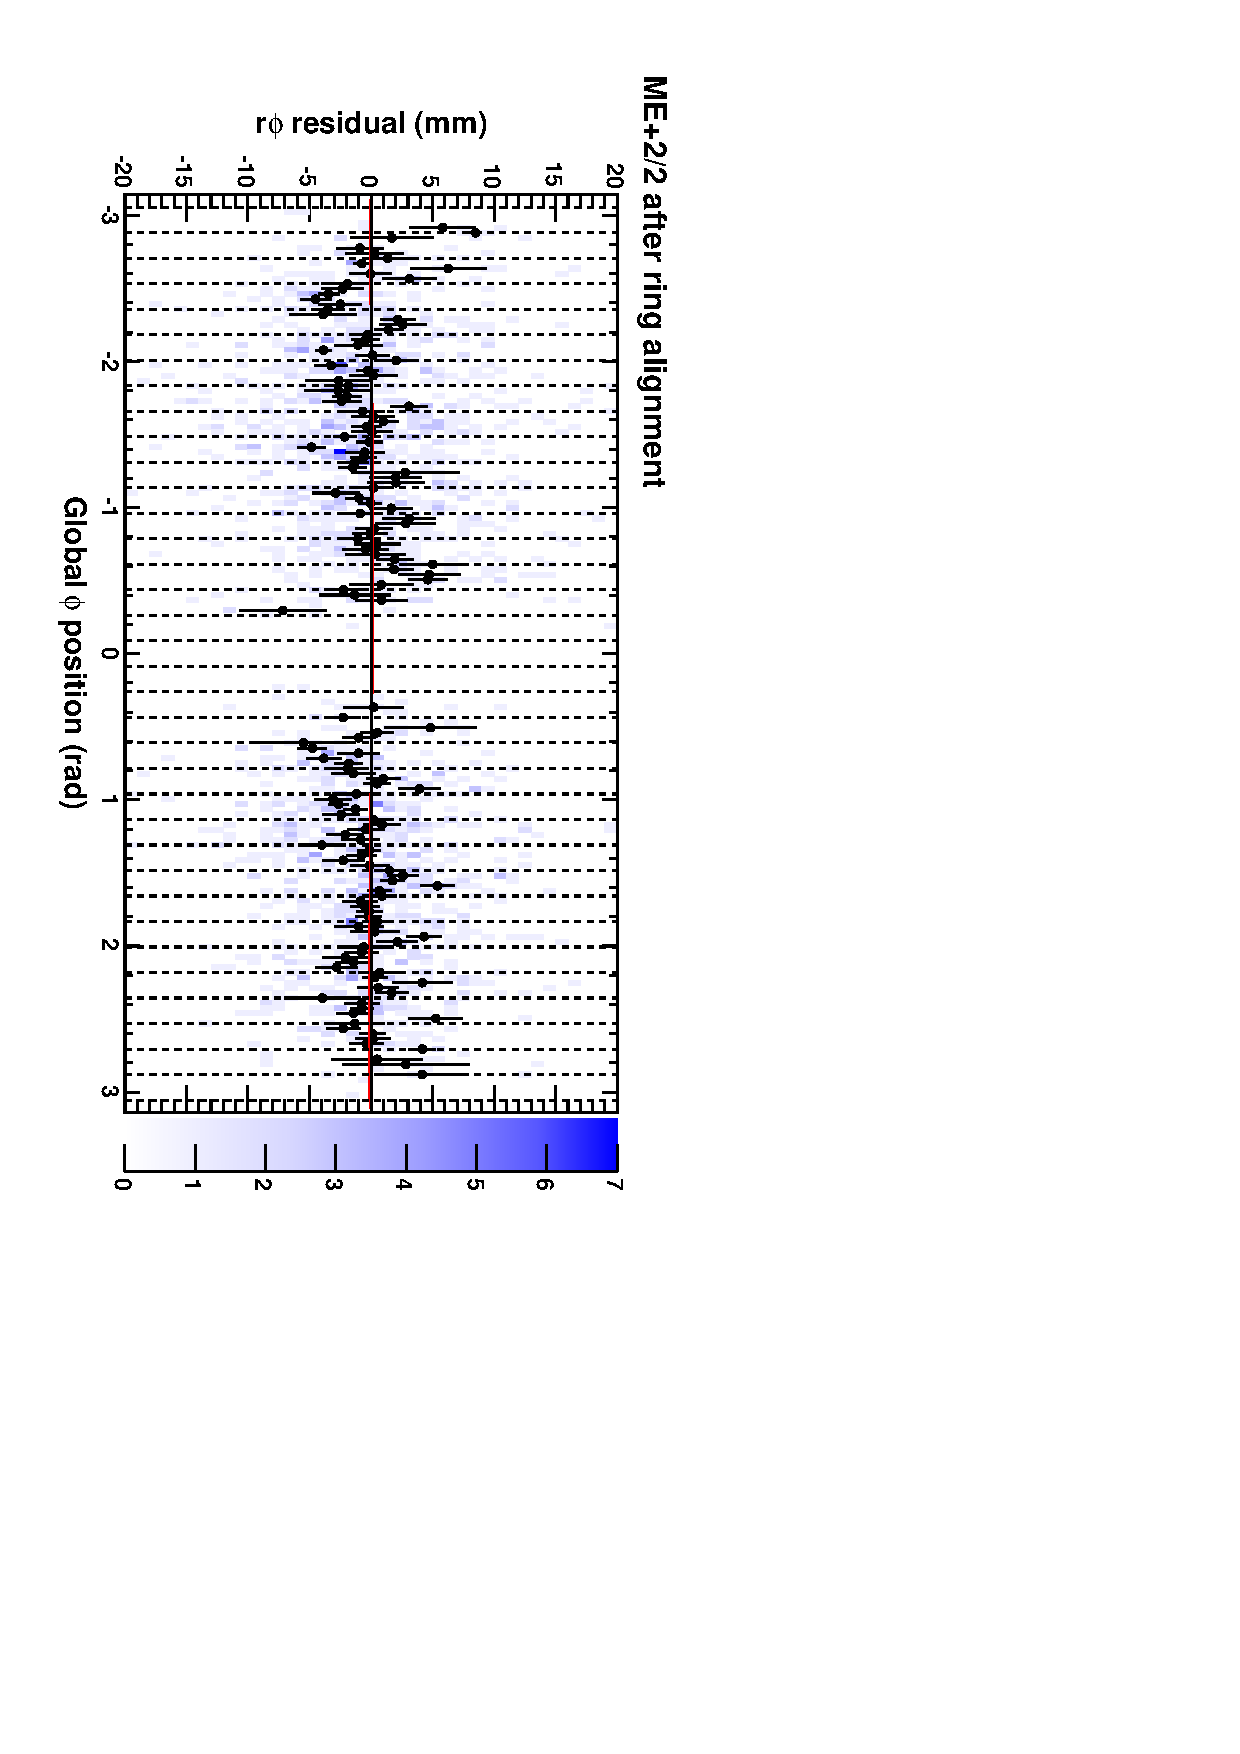
\includegraphics[height=\linewidth, angle=90]{ringfits_after/mep22.pdf}
\column{0.3\linewidth}
\begin{itemize}
\item Color scale is 2-D plot
\item Black points are a profile (averages in vertical bins)
\item Red line is fit to 2-D data
\end{itemize}
\end{columns}
\end{frame}

\begin{frame}
\frametitle{Ring fits: ME$+$3/1}
\vfill
\begin{columns}
\column{0.7\linewidth}
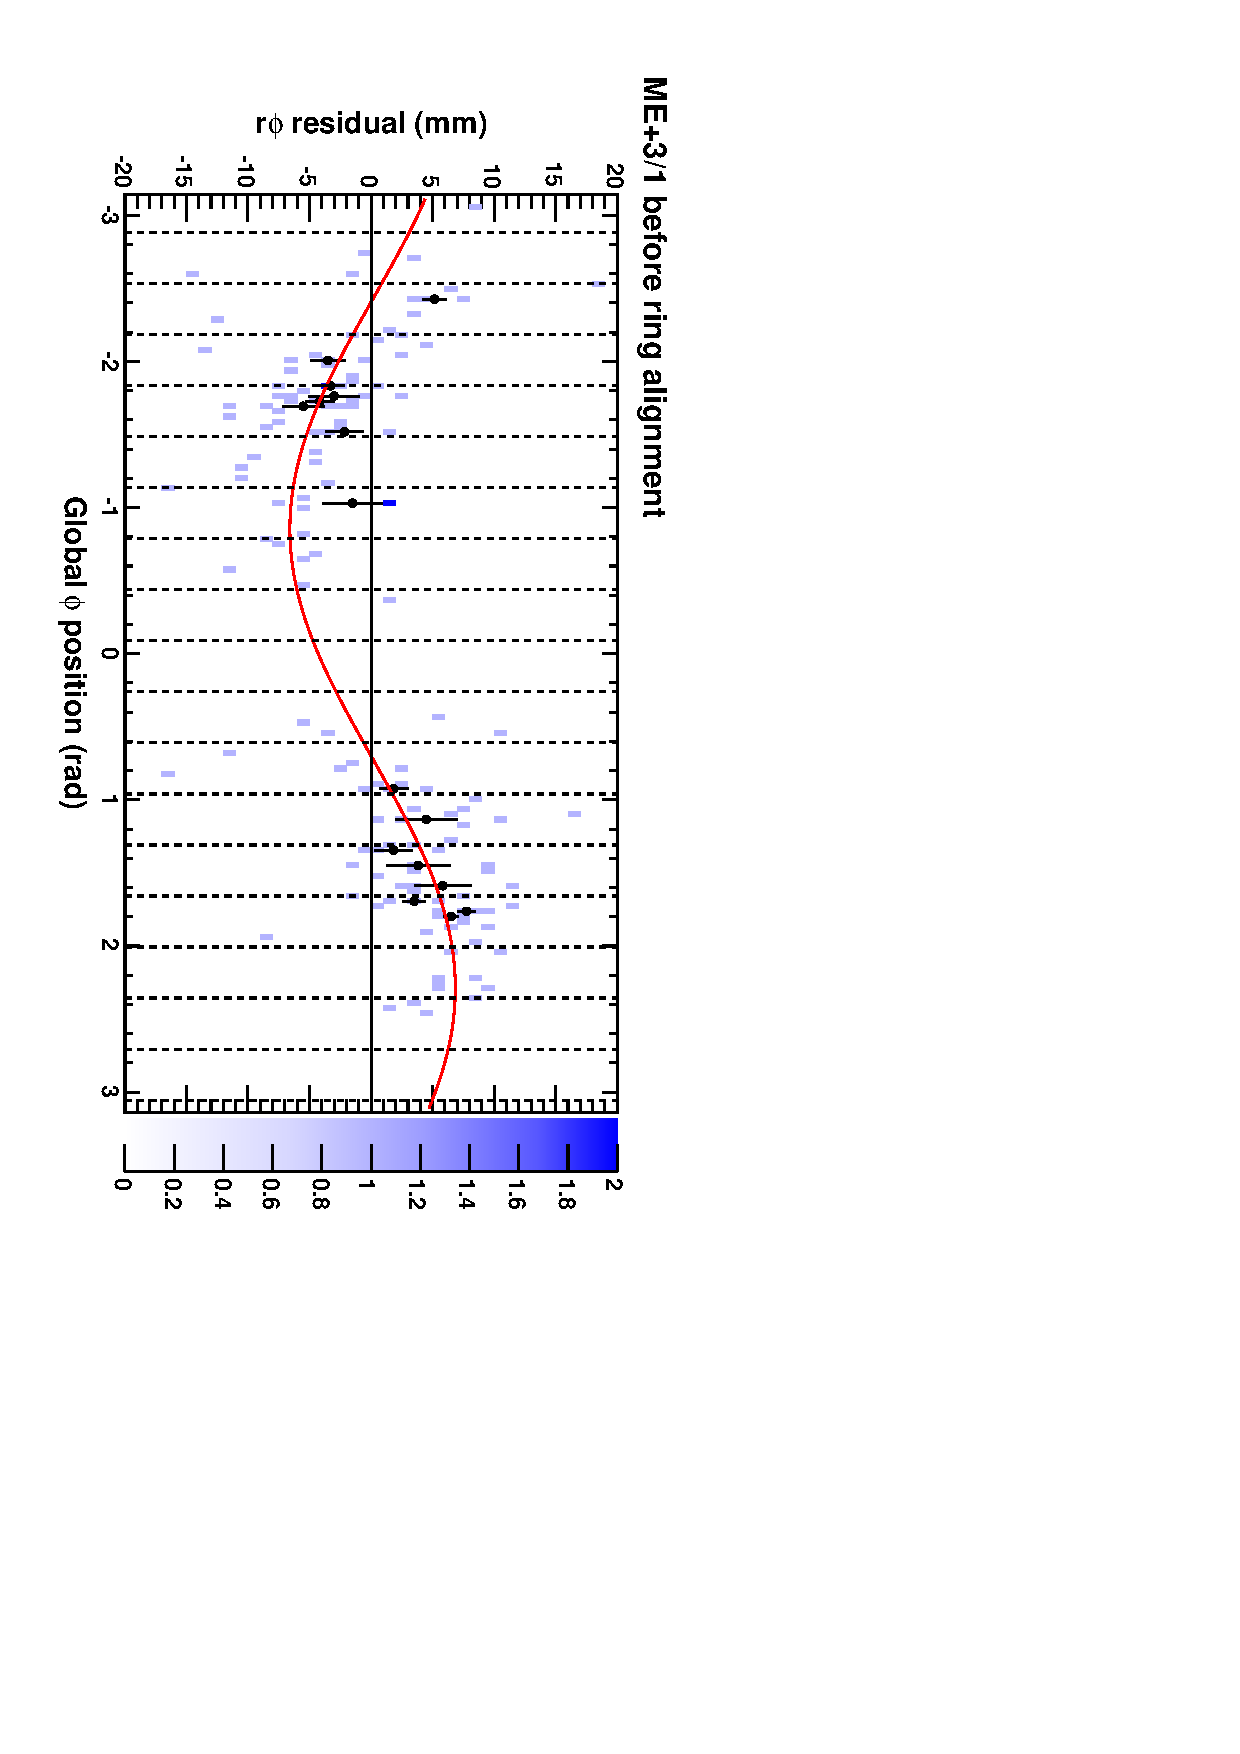
\includegraphics[height=\linewidth, angle=90]{ringfits_before/mep31.pdf}

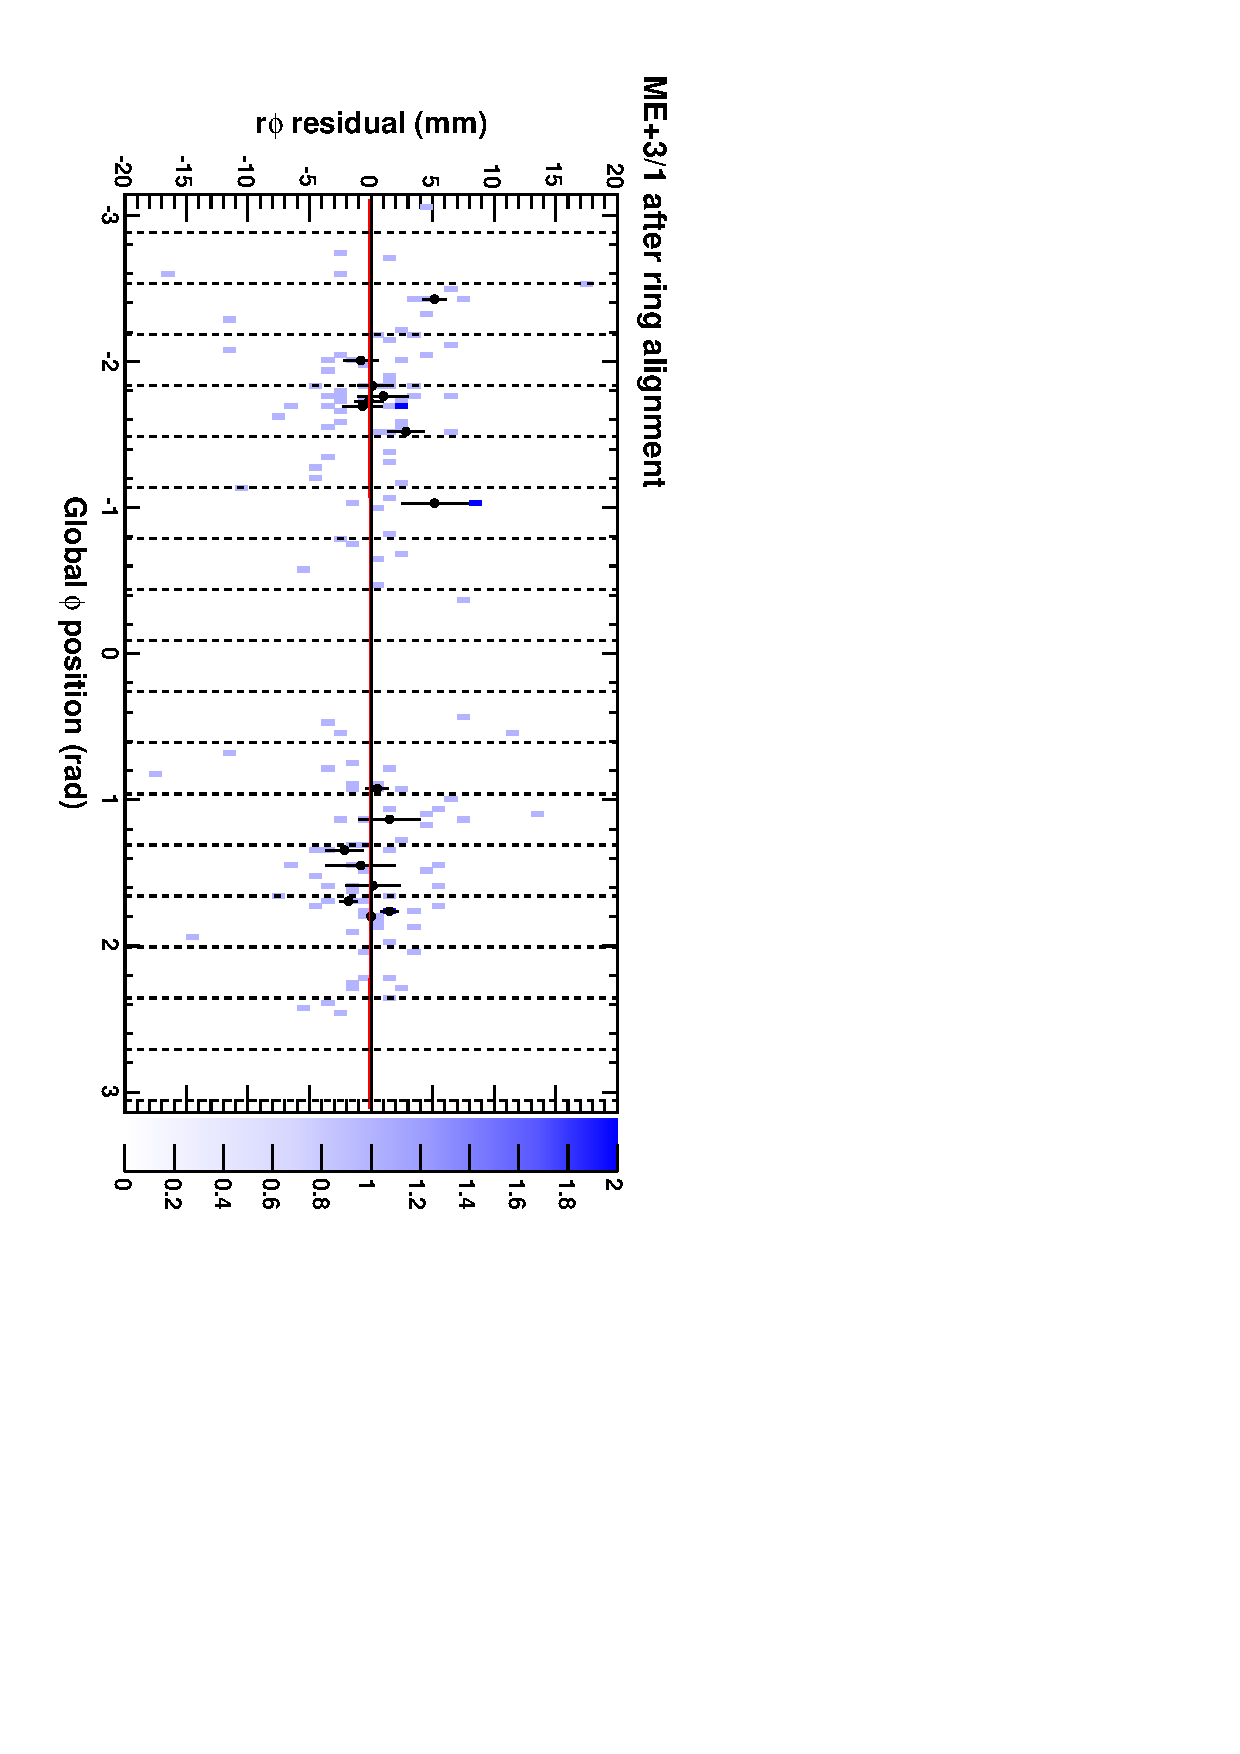
\includegraphics[height=\linewidth, angle=90]{ringfits_after/mep31.pdf}
\column{0.3\linewidth}
\begin{itemize}
\item Color scale is 2-D plot
\item Black points are a profile (averages in vertical bins)
\item Red line is fit to 2-D data
\end{itemize}
\end{columns}
\end{frame}

\begin{frame}
\frametitle{Ring fits: ME$+$3/2}
\vfill
\begin{columns}
\column{0.7\linewidth}
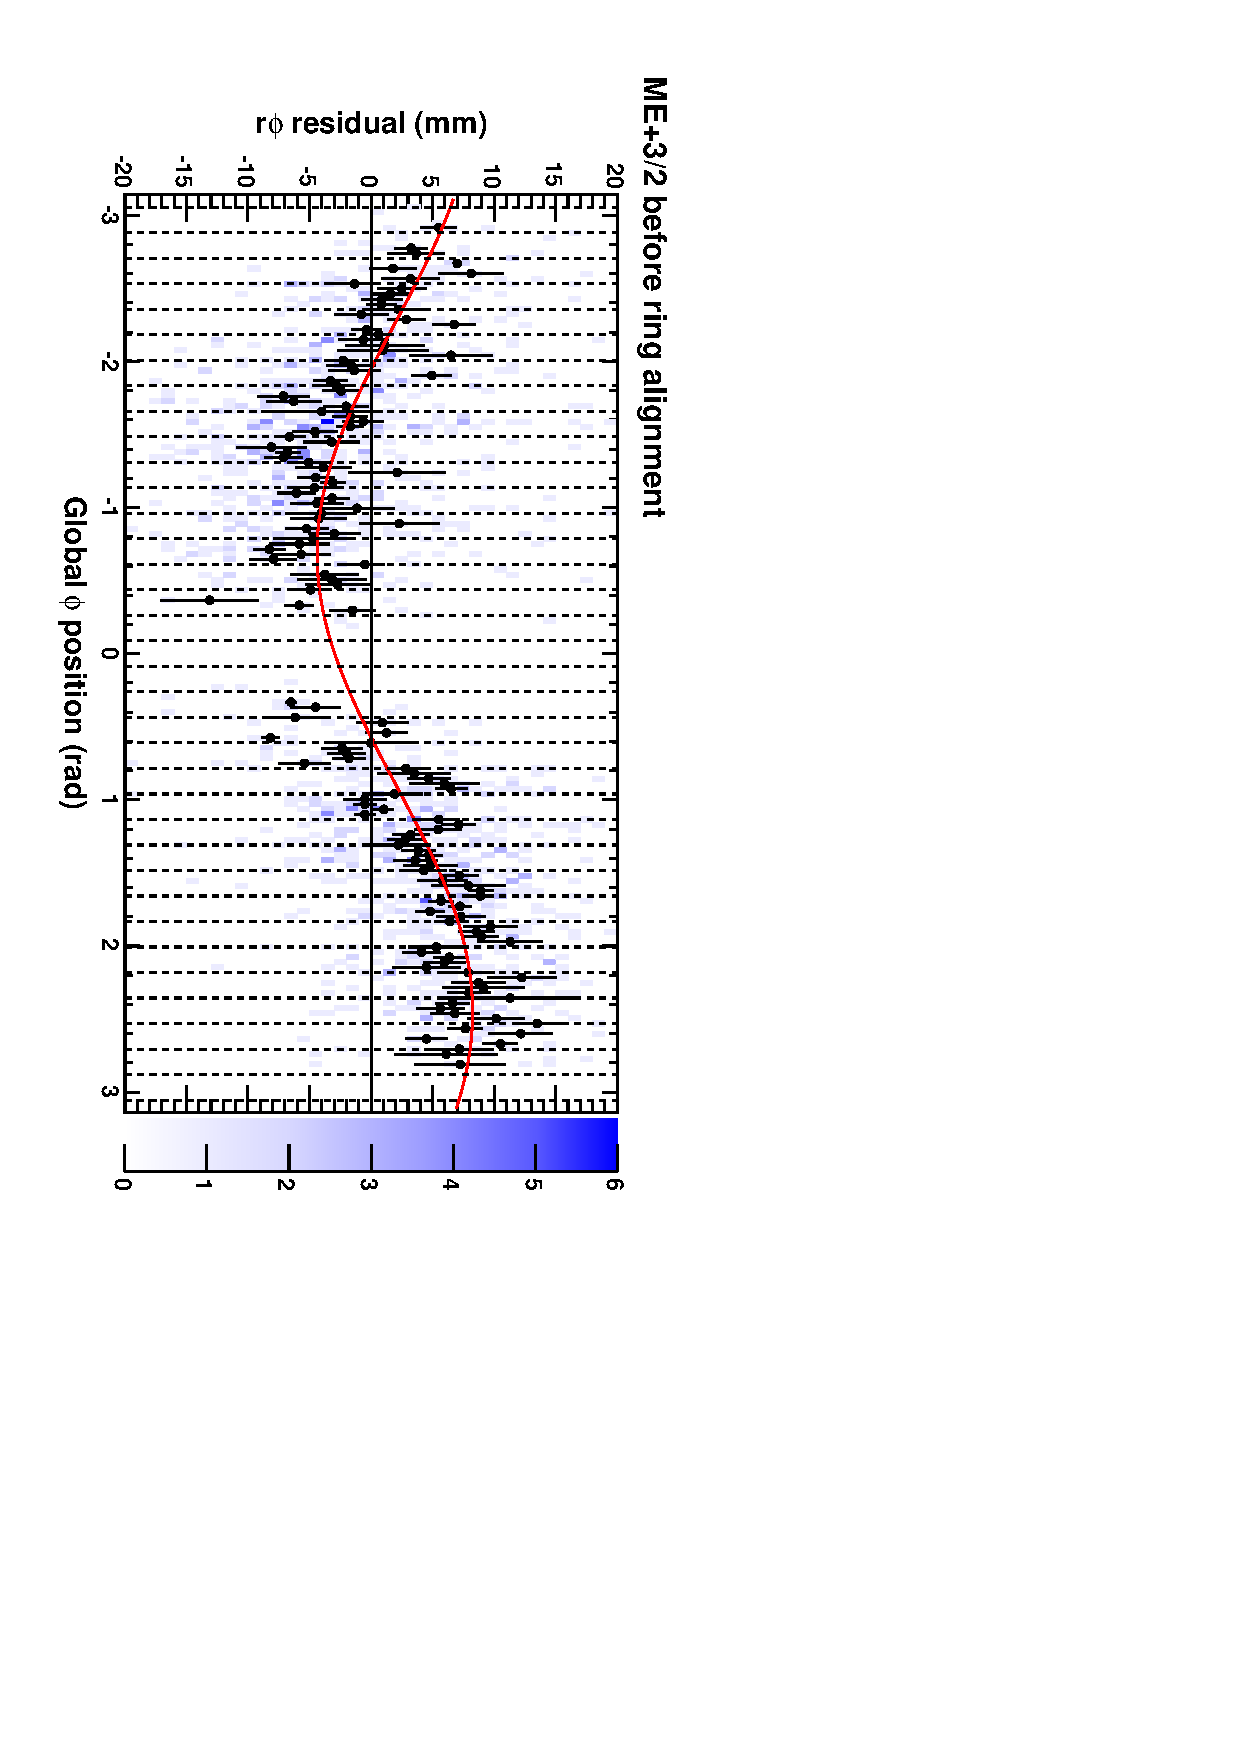
\includegraphics[height=\linewidth, angle=90]{ringfits_before/mep32.pdf}

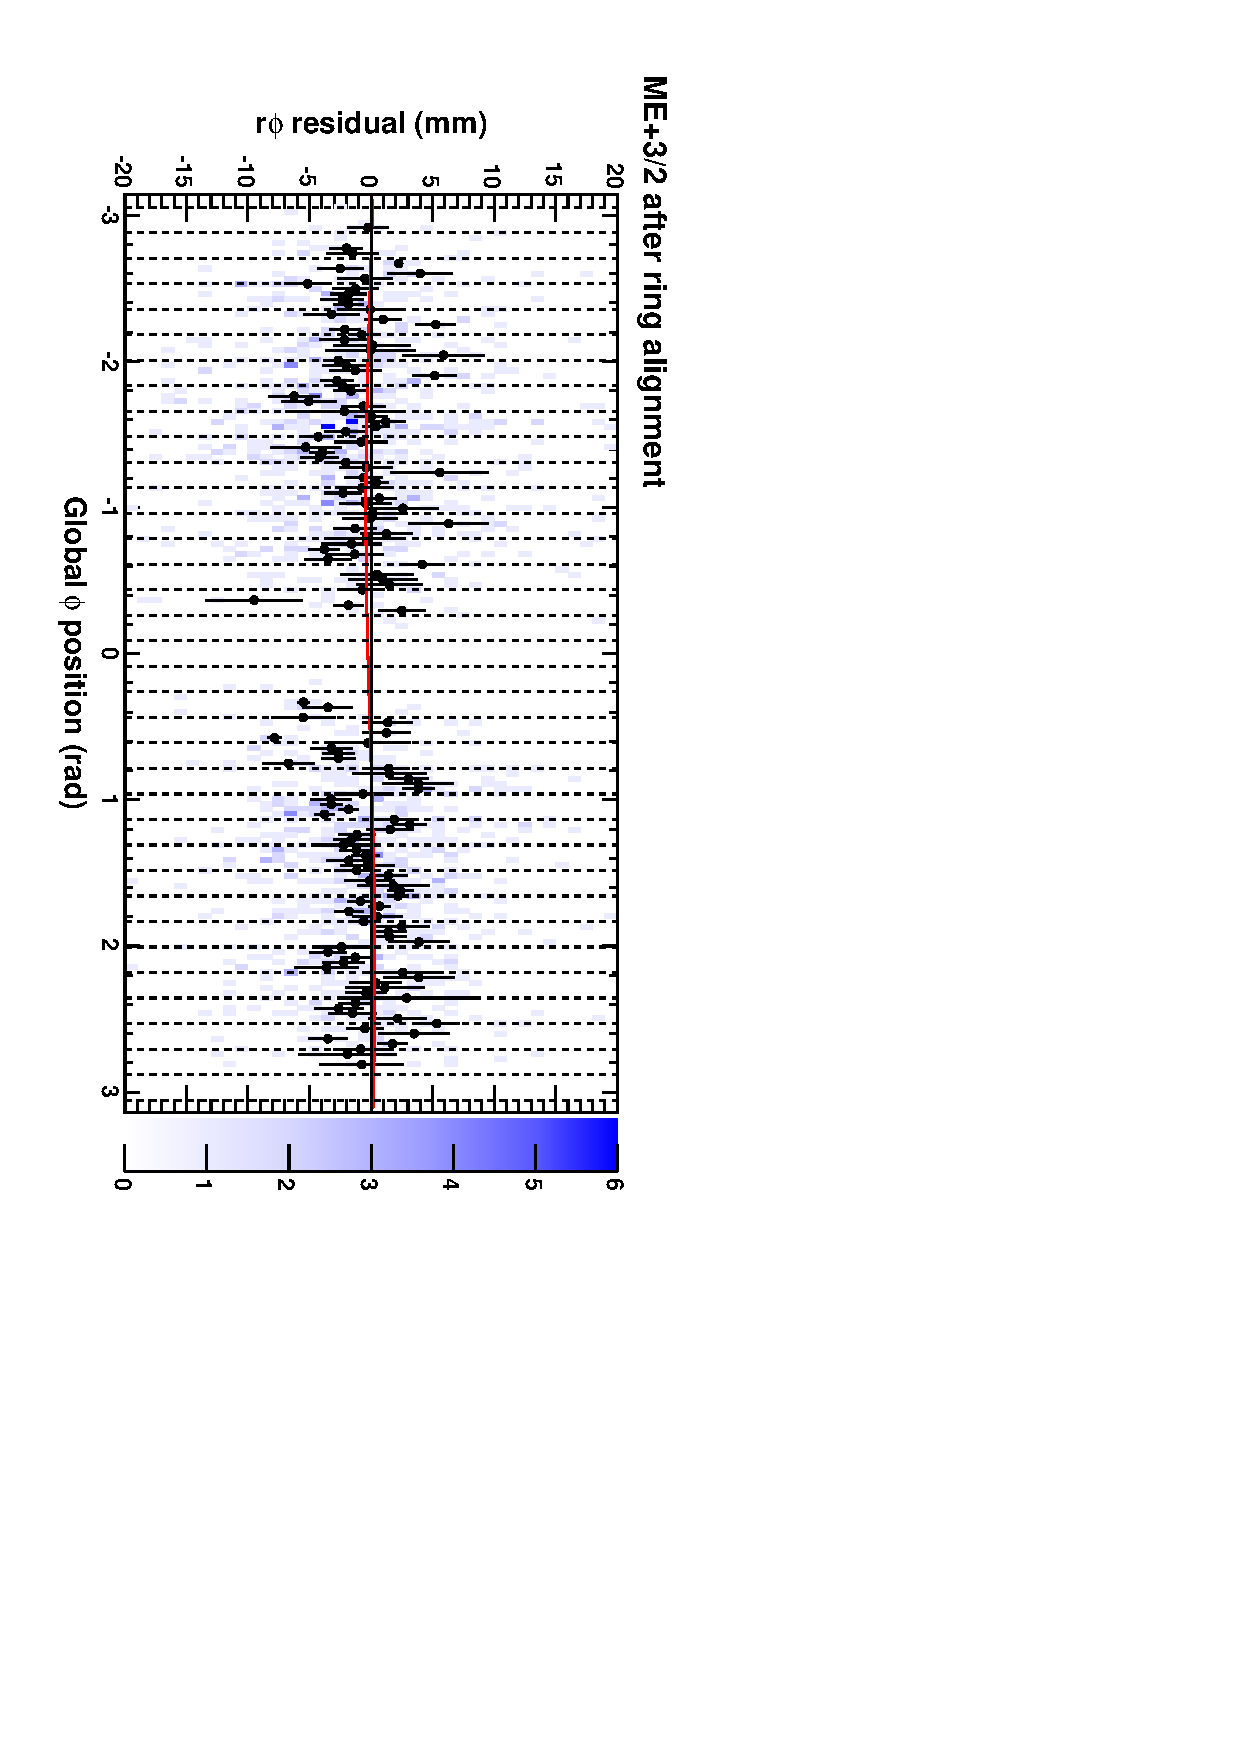
\includegraphics[height=\linewidth, angle=90]{ringfits_after/mep32.pdf}
\column{0.3\linewidth}
\begin{itemize}
\item Color scale is 2-D plot
\item Black points are a profile (averages in vertical bins)
\item Red line is fit to 2-D data
\end{itemize}
\end{columns}
\end{frame}

\begin{frame}
\frametitle{Ring fits: ME$+$4/1}
\vfill
\begin{columns}
\column{0.7\linewidth}
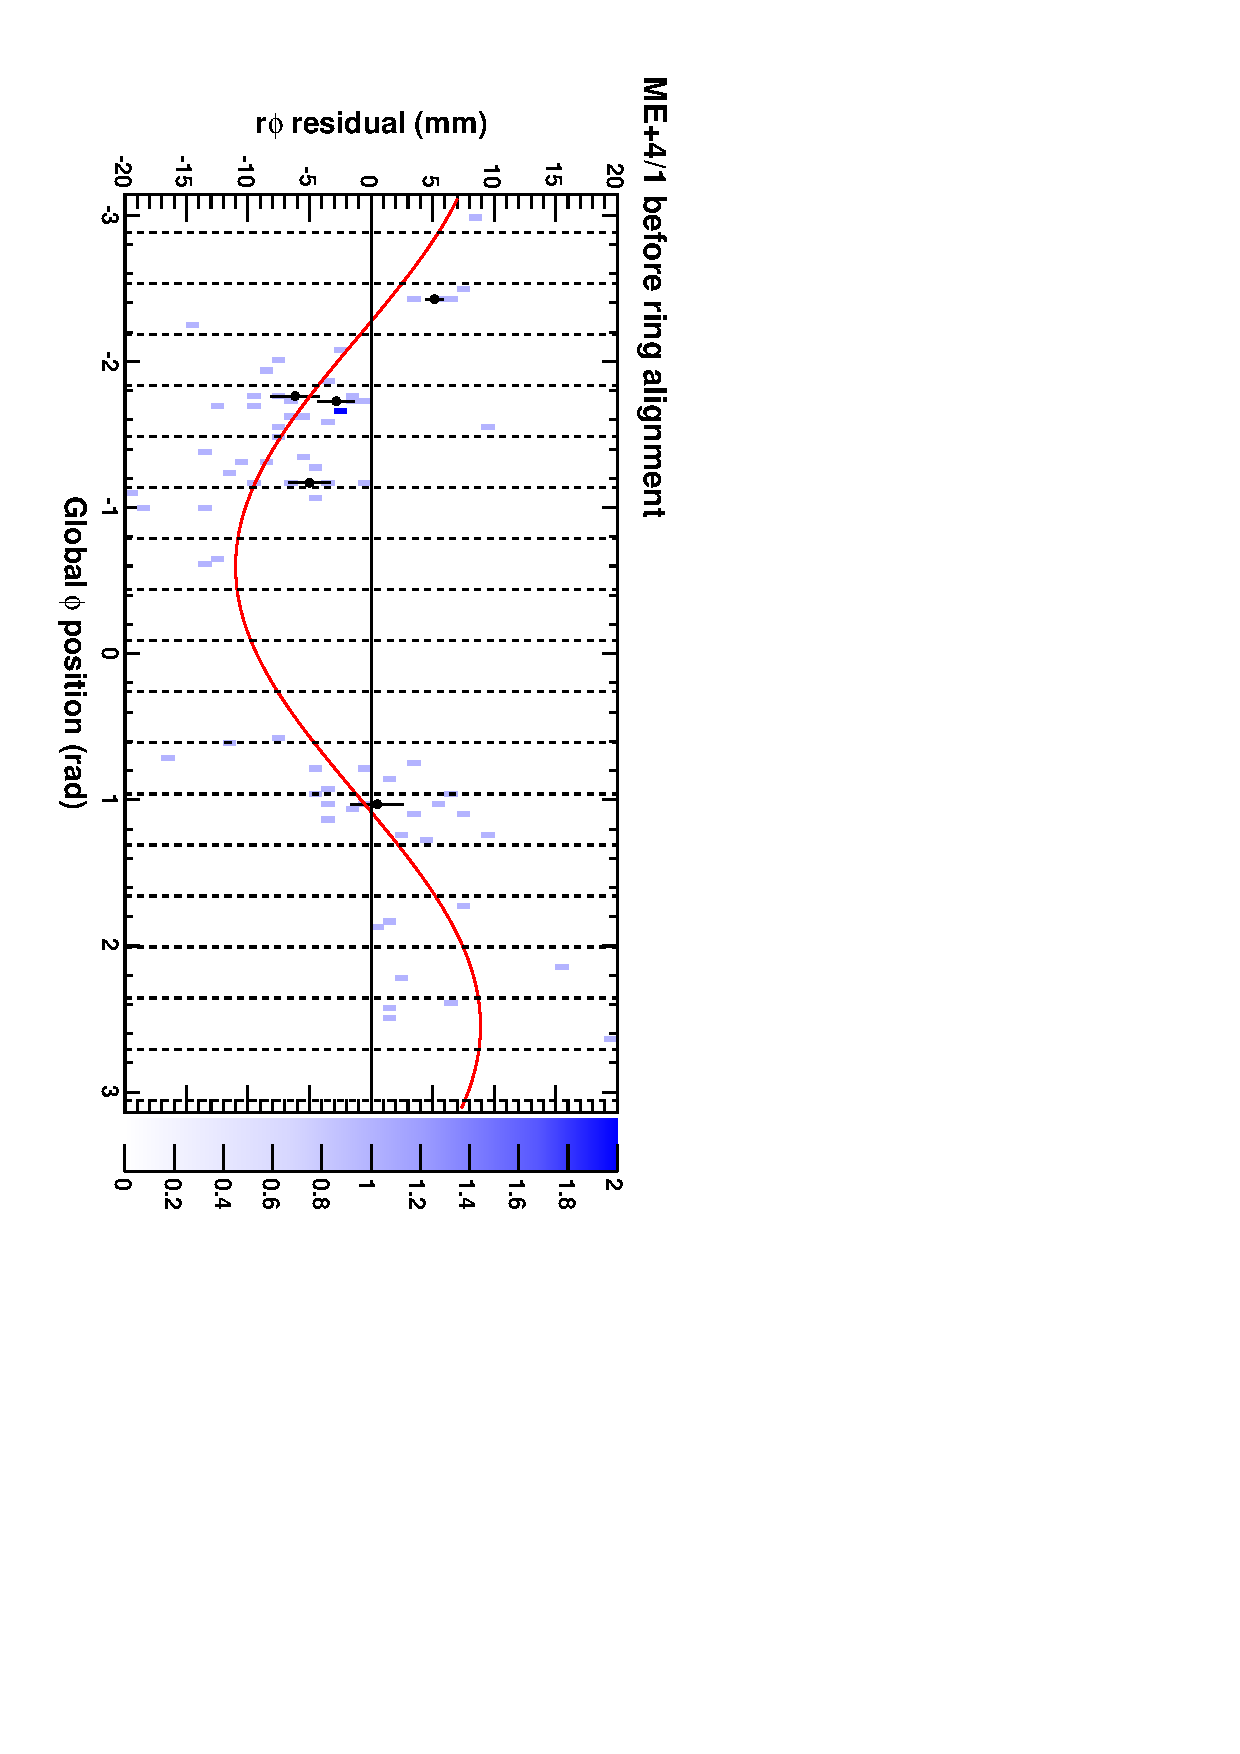
\includegraphics[height=\linewidth, angle=90]{ringfits_before/mep41.pdf}

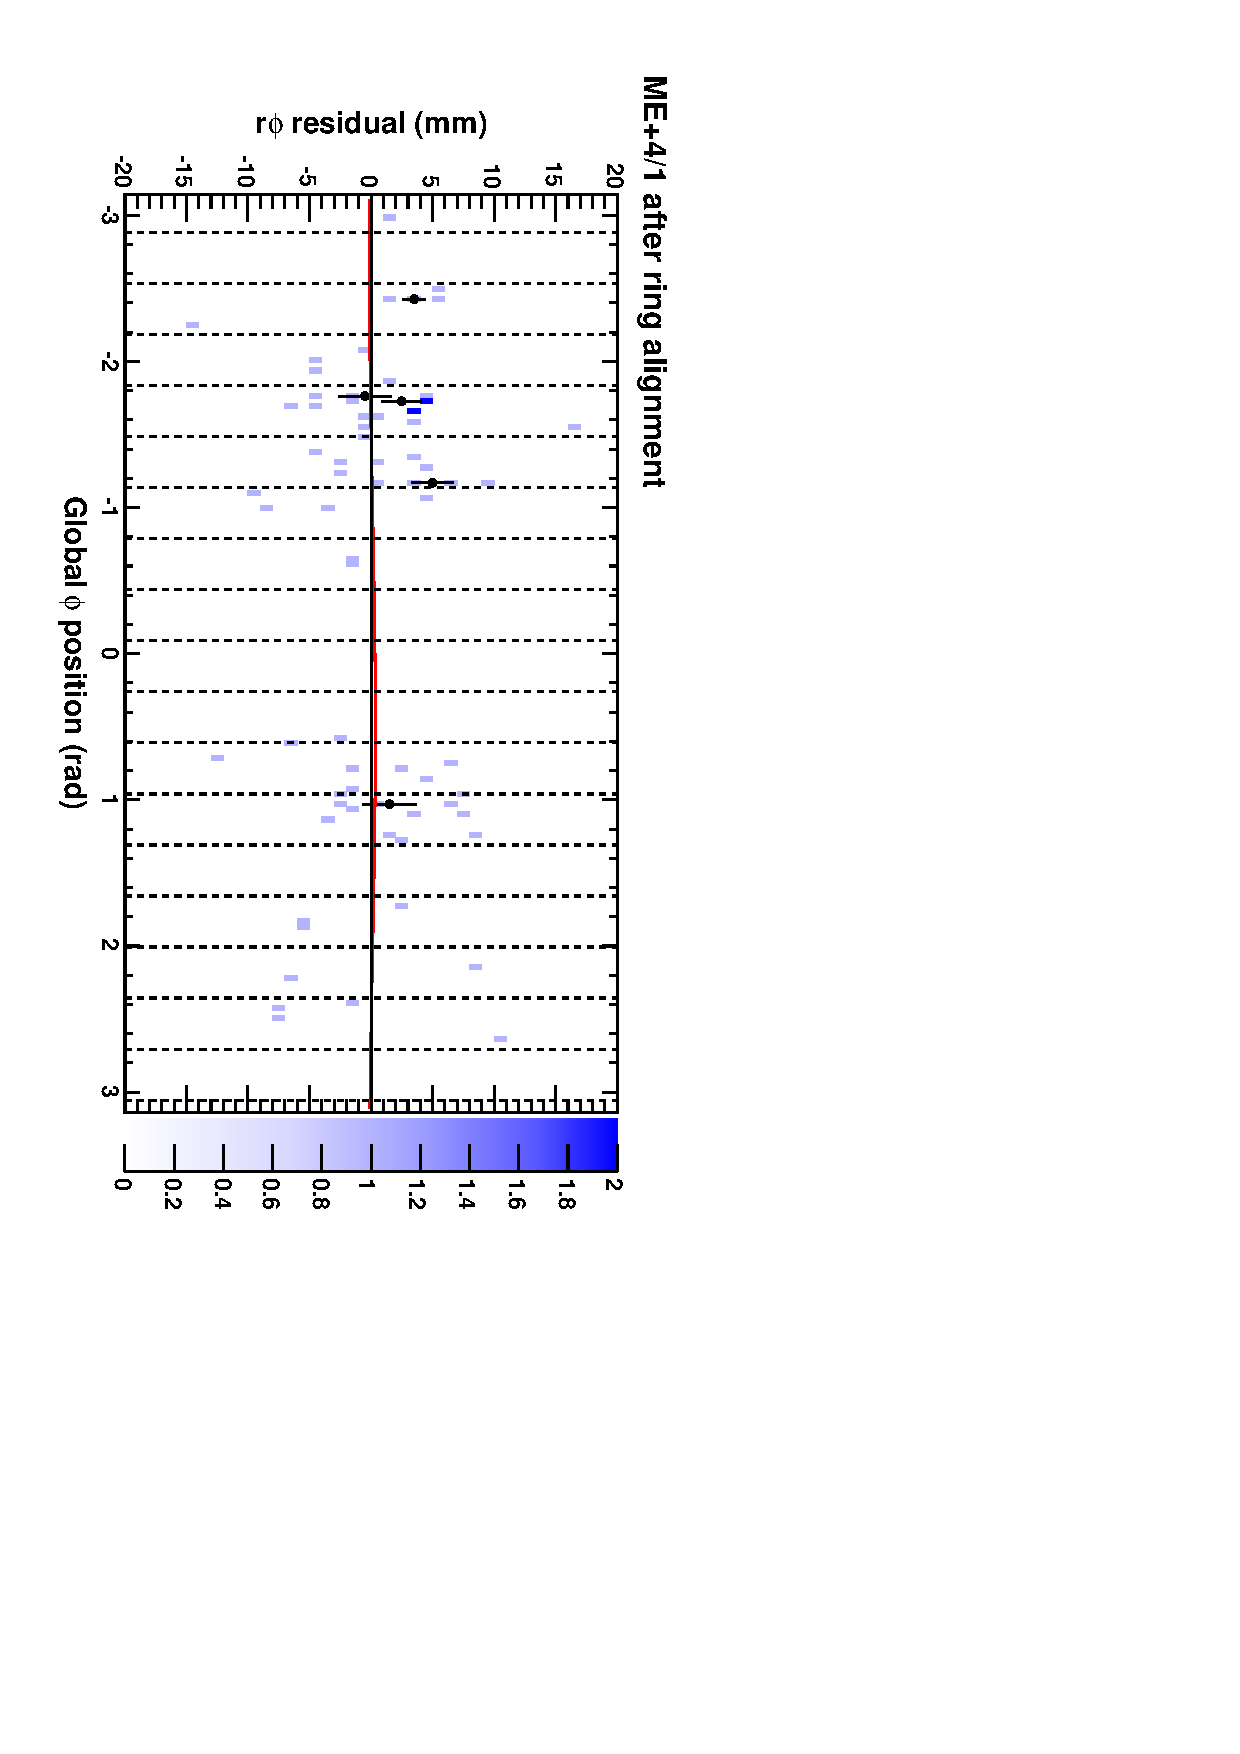
\includegraphics[height=\linewidth, angle=90]{ringfits_after/mep41.pdf}
\column{0.3\linewidth}
\begin{itemize}
\item Color scale is 2-D plot
\item Black points are a profile (averages in vertical bins)
\item Red line is fit to 2-D data
\end{itemize}
\end{columns}
\end{frame}

\begin{frame}
\frametitle{Table of ring corrections}
\begin{itemize}
\item Grouped items are physically connected to the same disk; values are correlated but not exactly equal within fitting errors
\item Large $\chi^2/\mbox{ndf}$ expected from incomplete chamber alignment
\end{itemize}

\scriptsize
\renewcommand{\arraystretch}{1.1}
\begin{tabular}{c | c c c c}
ring & $\delta_x$ (mm) & $\delta_y$ (mm) & $\delta_{\phi_z}$ (mrad) & $\chi^2/\mbox{ndf}$ \\\hline
ME$-$4/1 & $ 5.00$ $\pm$ $ 0.14$ & $-1.30$ $\pm$ $ 0.22$ & $ 1.57$ $\pm$ $ 0.05$ & 79.8998 \\\hline
ME$-$3/2 & $ 2.25$ $\pm$ $ 0.04$ & $-0.62$ $\pm$ $ 0.06$ & $ 1.85$ $\pm$ $ 0.01$ & 60.1288 \\
ME$-$3/1 & $ 4.16$ $\pm$ $ 0.12$ & $ 0.06$ $\pm$ $ 0.18$ & $ 2.12$ $\pm$ $ 0.04$ & 63.914 \\
ME$-$2/2 & $ 1.66$ $\pm$ $ 0.04$ & $ 1.29$ $\pm$ $ 0.05$ & $ 1.68$ $\pm$ $ 0.01$ & 52.9565 \\
ME$-$2/1 & $ 3.77$ $\pm$ $ 0.09$ & $-1.96$ $\pm$ $ 0.13$ & $ 2.18$ $\pm$ $ 0.03$ & 37.8555 \\\hline
ME$-$1/3 & $ 2.41$ $\pm$ $ 0.06$ & $ 1.43$ $\pm$ $ 0.09$ & $ 0.26$ $\pm$ $ 0.01$ & 45.2275 \\
ME$-$1/2 & $ 3.52$ $\pm$ $ 0.05$ & $-1.56$ $\pm$ $ 0.07$ & $ 0.85$ $\pm$ $ 0.01$ & 23.7824 \\
ME$-$1/1 & $ 2.93$ $\pm$ $ 0.09$ & $-2.90$ $\pm$ $ 0.13$ & $ 0.66$ $\pm$ $ 0.04$ & 5.31818 \\\hline
ME$+$1/1 & $ 4.95$ $\pm$ $ 0.08$ & $-1.93$ $\pm$ $ 0.11$ & $ 0.17$ $\pm$ $ 0.04$ & 11.9906 \\
ME$+$1/2 & $ 5.05$ $\pm$ $ 0.05$ & $ 0.81$ $\pm$ $ 0.07$ & $ 0.13$ $\pm$ $ 0.01$ & 22.0969 \\
ME$+$1/3 & $ 4.36$ $\pm$ $ 0.06$ & $ 3.22$ $\pm$ $ 0.08$ & $ 0.02$ $\pm$ $ 0.01$ & 38.1421 \\\hline
ME$+$2/1 & $ 4.56$ $\pm$ $ 0.08$ & $ 2.30$ $\pm$ $ 0.12$ & $ 0.18$ $\pm$ $ 0.03$ & 28.5622 \\
ME$+$2/2 & $ 4.28$ $\pm$ $ 0.04$ & $ 3.86$ $\pm$ $ 0.05$ & $-0.11$ $\pm$ $ 0.01$ & 47.6725 \\
ME$+$3/1 & $ 5.06$ $\pm$ $ 0.10$ & $ 4.42$ $\pm$ $ 0.17$ & $-0.05$ $\pm$ $ 0.03$ & 25.2588 \\
ME$+$3/2 & $ 4.01$ $\pm$ $ 0.04$ & $ 4.88$ $\pm$ $ 0.06$ & $-0.37$ $\pm$ $ 0.01$ & 60.8494 \\\hline
ME$+$4/1 & $ 5.58$ $\pm$ $ 0.15$ & $ 8.24$ $\pm$ $ 0.24$ & $ 0.40$ $\pm$ $ 0.05$ & 31.3307 \\
\end{tabular}
\end{frame}

\begin{frame}
\frametitle{About statistics}
\begin{itemize}
\item This reprocessed dataset was based on the following runs:

\mbox{\hspace{-1.25 cm}\begin{minipage}{1.15\linewidth}
\tiny
108483 108498 108516 108521 108526 108562 108597 108624 108645 108662
108666 108669 108671 108681 108686 108706 108712 108720 108731 108741
108787 108794 108819 108841 108852 108856 108859 108866 108873 108878
108889 108934 108959 109011 109024 109032 109035 109037 109039 109043
109046 109049 109112 109131 109132 109134 109142 109143 109144 109145
109146 109148 109203 109216 109261 109272 109288 109295 109305 109316
109319 109341 109354 109367 109403 109410 109411 109415 109418 109419
109425 109426 109441 109446 109450 109453 109456 109457 109459 109467
109468 109470 109472 109474 109490 109504 109508 109519 109524 109559
109562 109573 109575 109578 109584 109586 109589 109603 109606 109616
109624 109644 109654 109673 109703 109705 109706 109710 109712 109715
109718 109721 109747 109784 109805 109807 109810 109812 109815 109817
109822 109826 109829 109839 109844 109861 109885 109887 109897 109902
109904 109905 109908 109910 109911 109912 109920 109933 109935 109943
109950 109956 109961 109989 110000 110004 110007 110012 110092 110128
110133 110163 110169 110177 110182 110190 110193 110195 110213 110217
110219 110232 110286 110290 110308 110315 110323 110334 110341 110388
110393 110394 110395 110397 110407 110409 110419 110428 110431 110437
110440 110452 110467 110476 110485 110490 110496 110508 110514 110518
110520 110532 110535 110540 110546 110683 110685 110686 110689 110690
110692 110695 110697 110699 110703 110708 110722 110751 110756 110784
110832 110835 110842 110846 110873 110878 110891 110894 110900 110916
110921 110924 110952 110954 110955 110958 110972 110987 110998 111009
111017 111023 111030 111033 111035 111043 111045 111047 111101 111111
111129 111130 111138 111142 111143 111144 111145 111146 112009 112012
112013 112020 112043 112092 112101 112141 112205 112213 112215 112218
112222 112231 112233 112237 112248 112252 112255 112257 112265 112275
112281 112309 112323 112331 112341 112347 112360 112377 112381 112385
\end{minipage}}

\item The number of tracks passing cuts is: 8251

\end{itemize}

\vfill
\hspace{-0.83 cm} \textcolor{darkblue}{\Large Convergence}
\begin{itemize}
\item All chambers converged with $|\delta_{r\phi}| < 1$~mm
  $|\delta_{\phi_y}|$, $|\delta_{\phi_z}| < 1$~mrad \mbox{except\hspace{-1 cm}}
\begin{itemize}
\item ME$+$3/2, chamber 14
\item ME$-$1/2, chamber 25 and 31
\item ME$-$3/2, chamber 32
\end{itemize}
\end{itemize}
\end{frame}

\begin{frame}
\frametitle{On the following pages}
\begin{itemize}\setlength{\itemsep}{0.5 cm}
\item Lists of values of all chamber positions
\item Map plots (both $r\phi$ and $d(r\phi)/dz$ residuals versus $\phi$ and $R$ with dashed lines at chamber boundaries)
\item Fit functions (residuals and best-fit projected onto several axes)
\end{itemize}

\vfill
\hspace{-0.83 cm} \textcolor{darkblue}{\Large Where to find the constants}
\vspace{0.2 cm}
{\tiny \bf /afs/cern.ch/user/p/pivarski/public/CSCAlignmentRcd\_CRAFT09\_PG-hardware-globalMuons\_31X\_v1\_offline.db}

\begin{itemize}
\item tag ``CSCAlignmentRcd'': the aligned geometry
\item tag ``CSCAlignmentErrorRcd'': 0 for aligned chambers, 1000~cm for no track-based alignment step
\item ignore tags ``DTAlignmentRcd'' and ``DTAlignmentErrorRcd''
\end{itemize}

\label{numpages}
\end{frame}

\begin{frame}
\frametitle{All the values}
\tiny

All values relative to ideal, alternating $x$, $y$, $z$ (mm) and $\phi_x$, $\phi_y$, $\phi_z$ (mrad)

Columns: PG $+$ hardware, same $+$ global adjustment, \textcolor{red}{same $+$ track-based chambers}

\hfill (color applied only if chamber was aligned)

\vfill
\renewcommand{\arraystretch}{1.1}
\begin{tabular}{r | c | c | c}
station, chamber & $x$ or $\phi_x$ & $y$ or $\phi_y$ & $z$ or $\phi_z$ \\\hline
$+$1/1, 01 & $+0.00$\hspace{0.1 cm}$-1.62$\hspace{0.1 cm}\textcolor{black}{$-1.62$} & $+0.00$\hspace{0.1 cm}$+4.95$\hspace{0.1 cm}\textcolor{black}{$+4.95$} & $+17.57$\hspace{0.1 cm}$+17.57$\hspace{0.1 cm}\textcolor{black}{$+17.57$} \\
           & $+0.00$\hspace{0.1 cm}$+0.00$\hspace{0.1 cm}\textcolor{black}{$+0.00$} & $-0.00$\hspace{0.1 cm}$-0.00$\hspace{0.1 cm}\textcolor{black}{$-0.00$} & $-0.00$\hspace{0.1 cm}$-0.17$\hspace{0.1 cm}\textcolor{black}{$-0.17$} \\
$+$1/1, 02 & $+0.00$\hspace{0.1 cm}$-2.45$\hspace{0.1 cm}\textcolor{black}{$-2.45$} & $+0.00$\hspace{0.1 cm}$+4.54$\hspace{0.1 cm}\textcolor{black}{$+4.54$} & $+19.44$\hspace{0.1 cm}$+19.44$\hspace{0.1 cm}\textcolor{black}{$+19.44$} \\
           & $+0.00$\hspace{0.1 cm}$+0.00$\hspace{0.1 cm}\textcolor{black}{$+0.00$} & $-0.00$\hspace{0.1 cm}$-0.00$\hspace{0.1 cm}\textcolor{black}{$-0.00$} & $-0.00$\hspace{0.1 cm}$-0.17$\hspace{0.1 cm}\textcolor{black}{$-0.17$} \\
$+$1/1, 03 & $+0.00$\hspace{0.1 cm}$-3.20$\hspace{0.1 cm}\textcolor{black}{$-3.20$} & $+0.00$\hspace{0.1 cm}$+3.99$\hspace{0.1 cm}\textcolor{black}{$+3.99$} & $+19.44$\hspace{0.1 cm}$+19.44$\hspace{0.1 cm}\textcolor{black}{$+19.44$} \\
           & $+0.00$\hspace{0.1 cm}$+0.00$\hspace{0.1 cm}\textcolor{black}{$+0.00$} & $-0.00$\hspace{0.1 cm}$-0.00$\hspace{0.1 cm}\textcolor{black}{$-0.00$} & $-0.00$\hspace{0.1 cm}$-0.17$\hspace{0.1 cm}\textcolor{black}{$-0.17$} \\
$+$1/1, 04 & $+0.00$\hspace{0.1 cm}$-3.84$\hspace{0.1 cm}\textcolor{black}{$-3.84$} & $+0.00$\hspace{0.1 cm}$+3.32$\hspace{0.1 cm}\textcolor{black}{$+3.32$} & $+17.57$\hspace{0.1 cm}$+17.57$\hspace{0.1 cm}\textcolor{black}{$+17.57$} \\
           & $+0.00$\hspace{0.1 cm}$+0.00$\hspace{0.1 cm}\textcolor{black}{$+0.00$} & $-0.00$\hspace{0.1 cm}$-0.00$\hspace{0.1 cm}\textcolor{black}{$-0.00$} & $-0.00$\hspace{0.1 cm}$-0.17$\hspace{0.1 cm}\textcolor{black}{$-0.17$} \\
$+$1/1, 05 & $+0.00$\hspace{0.1 cm}$-4.36$\hspace{0.1 cm}\textcolor{black}{$-4.36$} & $+0.00$\hspace{0.1 cm}$+2.55$\hspace{0.1 cm}\textcolor{black}{$+2.55$} & $+17.57$\hspace{0.1 cm}$+17.57$\hspace{0.1 cm}\textcolor{black}{$+17.57$} \\
           & $+0.00$\hspace{0.1 cm}$+0.00$\hspace{0.1 cm}\textcolor{black}{$+0.00$} & $-0.00$\hspace{0.1 cm}$-0.00$\hspace{0.1 cm}\textcolor{black}{$-0.00$} & $-0.00$\hspace{0.1 cm}$-0.17$\hspace{0.1 cm}\textcolor{black}{$-0.17$} \\
$+$1/1, 06 & $+0.00$\hspace{0.1 cm}$-4.73$\hspace{0.1 cm}\textcolor{black}{$-4.73$} & $+0.00$\hspace{0.1 cm}$+1.71$\hspace{0.1 cm}\textcolor{black}{$+1.71$} & $+17.57$\hspace{0.1 cm}$+17.57$\hspace{0.1 cm}\textcolor{black}{$+17.57$} \\
           & $+0.00$\hspace{0.1 cm}$+0.00$\hspace{0.1 cm}\textcolor{black}{$+0.00$} & $-0.00$\hspace{0.1 cm}$-0.00$\hspace{0.1 cm}\textcolor{black}{$-0.00$} & $-0.00$\hspace{0.1 cm}$-0.17$\hspace{0.1 cm}\textcolor{black}{$-0.17$} \\
$+$1/1, 07 & $+0.00$\hspace{0.1 cm}$-4.95$\hspace{0.1 cm}\textcolor{black}{$-4.95$} & $+0.00$\hspace{0.1 cm}$+0.81$\hspace{0.1 cm}\textcolor{black}{$+0.81$} & $+17.57$\hspace{0.1 cm}$+17.57$\hspace{0.1 cm}\textcolor{black}{$+17.57$} \\
           & $+0.00$\hspace{0.1 cm}$+0.00$\hspace{0.1 cm}\textcolor{black}{$+0.00$} & $+0.00$\hspace{0.1 cm}$+0.00$\hspace{0.1 cm}\textcolor{black}{$+0.00$} & $-0.00$\hspace{0.1 cm}$-0.17$\hspace{0.1 cm}\textcolor{black}{$-0.17$} \\
$+$1/1, 08 & $+0.00$\hspace{0.1 cm}$-5.01$\hspace{0.1 cm}\textcolor{black}{$-5.01$} & $+0.00$\hspace{0.1 cm}$-0.12$\hspace{0.1 cm}\textcolor{black}{$-0.12$} & $+21.00$\hspace{0.1 cm}$+21.00$\hspace{0.1 cm}\textcolor{black}{$+21.00$} \\
           & $+0.00$\hspace{0.1 cm}$+0.00$\hspace{0.1 cm}\textcolor{black}{$+0.00$} & $+0.00$\hspace{0.1 cm}$+0.00$\hspace{0.1 cm}\textcolor{black}{$+0.00$} & $-0.00$\hspace{0.1 cm}$-0.17$\hspace{0.1 cm}\textcolor{black}{$-0.17$} \\
$+$1/1, 09 & $-0.00$\hspace{0.1 cm}$-4.91$\hspace{0.1 cm}\textcolor{black}{$-4.91$} & $+0.00$\hspace{0.1 cm}$-1.04$\hspace{0.1 cm}\textcolor{black}{$-1.04$} & $+21.00$\hspace{0.1 cm}$+21.00$\hspace{0.1 cm}\textcolor{black}{$+21.00$} \\
           & $+0.00$\hspace{0.1 cm}$+0.00$\hspace{0.1 cm}\textcolor{black}{$+0.00$} & $+0.00$\hspace{0.1 cm}$+0.00$\hspace{0.1 cm}\textcolor{black}{$+0.00$} & $-0.00$\hspace{0.1 cm}$-0.17$\hspace{0.1 cm}\textcolor{black}{$-0.17$} \\
$+$1/1, 10 & $-0.00$\hspace{0.1 cm}$-4.65$\hspace{0.1 cm}\textcolor{black}{$-4.65$} & $+0.00$\hspace{0.1 cm}$-1.93$\hspace{0.1 cm}\textcolor{black}{$-1.93$} & $+17.57$\hspace{0.1 cm}$+17.57$\hspace{0.1 cm}\textcolor{black}{$+17.57$} \\
           & $+0.00$\hspace{0.1 cm}$+0.00$\hspace{0.1 cm}\textcolor{black}{$+0.00$} & $+0.00$\hspace{0.1 cm}$+0.00$\hspace{0.1 cm}\textcolor{black}{$+0.00$} & $-0.00$\hspace{0.1 cm}$-0.17$\hspace{0.1 cm}\textcolor{black}{$-0.17$} \\
$+$1/1, 11 & $-0.00$\hspace{0.1 cm}$-4.24$\hspace{0.1 cm}\textcolor{black}{$-4.24$} & $+0.00$\hspace{0.1 cm}$-2.76$\hspace{0.1 cm}\textcolor{black}{$-2.76$} & $+17.57$\hspace{0.1 cm}$+17.57$\hspace{0.1 cm}\textcolor{black}{$+17.57$} \\
           & $+0.00$\hspace{0.1 cm}$+0.00$\hspace{0.1 cm}\textcolor{black}{$+0.00$} & $+0.00$\hspace{0.1 cm}$+0.00$\hspace{0.1 cm}\textcolor{black}{$+0.00$} & $+0.00$\hspace{0.1 cm}$-0.17$\hspace{0.1 cm}\textcolor{black}{$-0.17$} \\
$+$1/1, 12 & $-0.00$\hspace{0.1 cm}$-3.69$\hspace{0.1 cm}\textcolor{black}{$-3.69$} & $+0.00$\hspace{0.1 cm}$-3.51$\hspace{0.1 cm}\textcolor{black}{$-3.51$} & $+17.57$\hspace{0.1 cm}$+17.57$\hspace{0.1 cm}\textcolor{black}{$+17.57$} \\
           & $+0.00$\hspace{0.1 cm}$+0.00$\hspace{0.1 cm}\textcolor{black}{$+0.00$} & $+0.00$\hspace{0.1 cm}$+0.00$\hspace{0.1 cm}\textcolor{black}{$+0.00$} & $+0.00$\hspace{0.1 cm}$-0.17$\hspace{0.1 cm}\textcolor{black}{$-0.17$} \\
\end{tabular}
\end{frame}

\begin{frame}
\frametitle{All the values}
\tiny

All values relative to ideal, alternating $x$, $y$, $z$ (mm) and $\phi_x$, $\phi_y$, $\phi_z$ (mrad)

Columns: PG $+$ hardware, same $+$ global adjustment, \textcolor{red}{same $+$ track-based chambers}

\hfill (color applied only if chamber was aligned)

\vfill
\renewcommand{\arraystretch}{1.1}
\begin{tabular}{r | c | c | c}
station, chamber & $x$ or $\phi_x$ & $y$ or $\phi_y$ & $z$ or $\phi_z$ \\\hline
$+$1/1, 13 & $-0.00$\hspace{0.1 cm}$-3.02$\hspace{0.1 cm}\textcolor{black}{$-3.02$} & $+0.00$\hspace{0.1 cm}$-4.15$\hspace{0.1 cm}\textcolor{black}{$-4.15$} & $+17.57$\hspace{0.1 cm}$+17.57$\hspace{0.1 cm}\textcolor{black}{$+17.57$} \\
           & $+0.00$\hspace{0.1 cm}$+0.00$\hspace{0.1 cm}\textcolor{black}{$+0.00$} & $+0.00$\hspace{0.1 cm}$+0.00$\hspace{0.1 cm}\textcolor{black}{$+0.00$} & $+0.00$\hspace{0.1 cm}$-0.17$\hspace{0.1 cm}\textcolor{black}{$-0.17$} \\
$+$1/1, 14 & $-0.00$\hspace{0.1 cm}$-2.25$\hspace{0.1 cm}\textcolor{black}{$-2.25$} & $+0.00$\hspace{0.1 cm}$-4.66$\hspace{0.1 cm}\textcolor{black}{$-4.66$} & $+22.18$\hspace{0.1 cm}$+22.18$\hspace{0.1 cm}\textcolor{black}{$+22.18$} \\
           & $+0.00$\hspace{0.1 cm}$+0.00$\hspace{0.1 cm}\textcolor{black}{$+0.00$} & $+0.00$\hspace{0.1 cm}$+0.00$\hspace{0.1 cm}\textcolor{black}{$+0.00$} & $+0.00$\hspace{0.1 cm}$-0.17$\hspace{0.1 cm}\textcolor{black}{$-0.17$} \\
$+$1/1, 15 & $-0.00$\hspace{0.1 cm}$-1.40$\hspace{0.1 cm}\textcolor{black}{$-1.40$} & $+0.00$\hspace{0.1 cm}$-5.03$\hspace{0.1 cm}\textcolor{black}{$-5.03$} & $+22.18$\hspace{0.1 cm}$+22.18$\hspace{0.1 cm}\textcolor{black}{$+22.18$} \\
           & $+0.00$\hspace{0.1 cm}$+0.00$\hspace{0.1 cm}\textcolor{black}{$+0.00$} & $+0.00$\hspace{0.1 cm}$+0.00$\hspace{0.1 cm}\textcolor{black}{$+0.00$} & $+0.00$\hspace{0.1 cm}$-0.17$\hspace{0.1 cm}\textcolor{black}{$-0.17$} \\
$+$1/1, 16 & $-0.00$\hspace{0.1 cm}$-0.50$\hspace{0.1 cm}\textcolor{black}{$-0.50$} & $+0.00$\hspace{0.1 cm}$-5.25$\hspace{0.1 cm}\textcolor{black}{$-5.25$} & $+17.57$\hspace{0.1 cm}$+17.57$\hspace{0.1 cm}\textcolor{black}{$+17.57$} \\
           & $+0.00$\hspace{0.1 cm}$+0.00$\hspace{0.1 cm}\textcolor{black}{$+0.00$} & $+0.00$\hspace{0.1 cm}$+0.00$\hspace{0.1 cm}\textcolor{black}{$+0.00$} & $+0.00$\hspace{0.1 cm}$-0.17$\hspace{0.1 cm}\textcolor{black}{$-0.17$} \\
$+$1/1, 17 & $-0.00$\hspace{0.1 cm}$+0.42$\hspace{0.1 cm}\textcolor{black}{$+0.42$} & $+0.00$\hspace{0.1 cm}$-5.31$\hspace{0.1 cm}\textcolor{black}{$-5.31$} & $+17.57$\hspace{0.1 cm}$+17.57$\hspace{0.1 cm}\textcolor{black}{$+17.57$} \\
           & $-0.00$\hspace{0.1 cm}$-0.00$\hspace{0.1 cm}\textcolor{black}{$-0.00$} & $+0.00$\hspace{0.1 cm}$+0.00$\hspace{0.1 cm}\textcolor{black}{$+0.00$} & $+0.00$\hspace{0.1 cm}$-0.17$\hspace{0.1 cm}\textcolor{black}{$-0.17$} \\
$+$1/1, 18 & $-0.00$\hspace{0.1 cm}$+1.35$\hspace{0.1 cm}\textcolor{black}{$+1.35$} & $-0.00$\hspace{0.1 cm}$-5.21$\hspace{0.1 cm}\textcolor{black}{$-5.21$} & $+17.57$\hspace{0.1 cm}$+17.57$\hspace{0.1 cm}\textcolor{black}{$+17.57$} \\
           & $-0.00$\hspace{0.1 cm}$-0.00$\hspace{0.1 cm}\textcolor{black}{$-0.00$} & $+0.00$\hspace{0.1 cm}$+0.00$\hspace{0.1 cm}\textcolor{black}{$+0.00$} & $-0.00$\hspace{0.1 cm}$-0.17$\hspace{0.1 cm}\textcolor{black}{$-0.17$} \\
$+$1/1, 19 & $-0.00$\hspace{0.1 cm}$+2.23$\hspace{0.1 cm}\textcolor{black}{$+2.23$} & $-0.00$\hspace{0.1 cm}$-4.95$\hspace{0.1 cm}\textcolor{black}{$-4.95$} & $+17.57$\hspace{0.1 cm}$+17.57$\hspace{0.1 cm}\textcolor{black}{$+17.57$} \\
           & $-0.00$\hspace{0.1 cm}$-0.00$\hspace{0.1 cm}\textcolor{black}{$-0.00$} & $+0.00$\hspace{0.1 cm}$+0.00$\hspace{0.1 cm}\textcolor{black}{$+0.00$} & $-0.00$\hspace{0.1 cm}$-0.17$\hspace{0.1 cm}\textcolor{black}{$-0.17$} \\
$+$1/1, 20 & $-0.00$\hspace{0.1 cm}$+3.07$\hspace{0.1 cm}\textcolor{black}{$+3.07$} & $-0.00$\hspace{0.1 cm}$-4.54$\hspace{0.1 cm}\textcolor{black}{$-4.54$} & $+17.47$\hspace{0.1 cm}$+17.47$\hspace{0.1 cm}\textcolor{black}{$+17.47$} \\
           & $-0.00$\hspace{0.1 cm}$-0.00$\hspace{0.1 cm}\textcolor{black}{$-0.00$} & $+0.00$\hspace{0.1 cm}$+0.00$\hspace{0.1 cm}\textcolor{black}{$+0.00$} & $-0.00$\hspace{0.1 cm}$-0.17$\hspace{0.1 cm}\textcolor{black}{$-0.17$} \\
$+$1/1, 21 & $+0.00$\hspace{0.1 cm}$+3.81$\hspace{0.1 cm}\textcolor{black}{$+3.81$} & $-0.00$\hspace{0.1 cm}$-3.99$\hspace{0.1 cm}\textcolor{black}{$-3.99$} & $+17.47$\hspace{0.1 cm}$+17.47$\hspace{0.1 cm}\textcolor{black}{$+17.47$} \\
           & $-0.00$\hspace{0.1 cm}$-0.00$\hspace{0.1 cm}\textcolor{black}{$-0.00$} & $+0.00$\hspace{0.1 cm}$+0.00$\hspace{0.1 cm}\textcolor{black}{$+0.00$} & $-0.00$\hspace{0.1 cm}$-0.17$\hspace{0.1 cm}\textcolor{black}{$-0.17$} \\
$+$1/1, 22 & $+0.00$\hspace{0.1 cm}$+4.45$\hspace{0.1 cm}\textcolor{black}{$+4.45$} & $-0.00$\hspace{0.1 cm}$-3.32$\hspace{0.1 cm}\textcolor{black}{$-3.32$} & $+17.57$\hspace{0.1 cm}$+17.57$\hspace{0.1 cm}\textcolor{black}{$+17.57$} \\
           & $-0.00$\hspace{0.1 cm}$-0.00$\hspace{0.1 cm}\textcolor{black}{$-0.00$} & $-0.00$\hspace{0.1 cm}$-0.00$\hspace{0.1 cm}\textcolor{black}{$-0.00$} & $-0.00$\hspace{0.1 cm}$-0.17$\hspace{0.1 cm}\textcolor{black}{$-0.17$} \\
$+$1/1, 23 & $+0.00$\hspace{0.1 cm}$+4.97$\hspace{0.1 cm}\textcolor{black}{$+4.97$} & $-0.00$\hspace{0.1 cm}$-2.55$\hspace{0.1 cm}\textcolor{black}{$-2.55$} & $+17.57$\hspace{0.1 cm}$+17.57$\hspace{0.1 cm}\textcolor{black}{$+17.57$} \\
           & $-0.00$\hspace{0.1 cm}$-0.00$\hspace{0.1 cm}\textcolor{black}{$-0.00$} & $-0.00$\hspace{0.1 cm}$-0.00$\hspace{0.1 cm}\textcolor{black}{$-0.00$} & $-0.00$\hspace{0.1 cm}$-0.17$\hspace{0.1 cm}\textcolor{black}{$-0.17$} \\
$+$1/1, 24 & $+0.00$\hspace{0.1 cm}$+5.34$\hspace{0.1 cm}\textcolor{black}{$+5.34$} & $-0.00$\hspace{0.1 cm}$-1.71$\hspace{0.1 cm}\textcolor{black}{$-1.71$} & $+17.57$\hspace{0.1 cm}$+17.57$\hspace{0.1 cm}\textcolor{black}{$+17.57$} \\
           & $-0.00$\hspace{0.1 cm}$-0.00$\hspace{0.1 cm}\textcolor{black}{$-0.00$} & $-0.00$\hspace{0.1 cm}$-0.00$\hspace{0.1 cm}\textcolor{black}{$-0.00$} & $-0.00$\hspace{0.1 cm}$-0.17$\hspace{0.1 cm}\textcolor{black}{$-0.17$} \\
\end{tabular}
\end{frame}

\begin{frame}
\frametitle{All the values}
\tiny

All values relative to ideal, alternating $x$, $y$, $z$ (mm) and $\phi_x$, $\phi_y$, $\phi_z$ (mrad)

Columns: PG $+$ hardware, same $+$ global adjustment, \textcolor{red}{same $+$ track-based chambers}

\hfill (color applied only if chamber was aligned)

\vfill
\renewcommand{\arraystretch}{1.1}
\begin{tabular}{r | c | c | c}
station, chamber & $x$ or $\phi_x$ & $y$ or $\phi_y$ & $z$ or $\phi_z$ \\\hline
$+$1/1, 25 & $+0.00$\hspace{0.1 cm}$+5.56$\hspace{0.1 cm}\textcolor{black}{$+5.56$} & $-0.00$\hspace{0.1 cm}$-0.81$\hspace{0.1 cm}\textcolor{black}{$-0.81$} & $+17.57$\hspace{0.1 cm}$+17.57$\hspace{0.1 cm}\textcolor{black}{$+17.57$} \\
           & $-0.00$\hspace{0.1 cm}$-0.00$\hspace{0.1 cm}\textcolor{black}{$-0.00$} & $-0.00$\hspace{0.1 cm}$-0.00$\hspace{0.1 cm}\textcolor{black}{$-0.00$} & $-0.00$\hspace{0.1 cm}$-0.17$\hspace{0.1 cm}\textcolor{black}{$-0.17$} \\
$+$1/1, 26 & $+0.00$\hspace{0.1 cm}$+5.62$\hspace{0.1 cm}\textcolor{black}{$+5.62$} & $-0.00$\hspace{0.1 cm}$+0.12$\hspace{0.1 cm}\textcolor{black}{$+0.12$} & $+14.05$\hspace{0.1 cm}$+14.05$\hspace{0.1 cm}\textcolor{black}{$+14.05$} \\
           & $-0.00$\hspace{0.1 cm}$-0.00$\hspace{0.1 cm}\textcolor{black}{$-0.00$} & $-0.00$\hspace{0.1 cm}$-0.00$\hspace{0.1 cm}\textcolor{black}{$-0.00$} & $-0.00$\hspace{0.1 cm}$-0.17$\hspace{0.1 cm}\textcolor{black}{$-0.17$} \\
$+$1/1, 27 & $+0.00$\hspace{0.1 cm}$+5.52$\hspace{0.1 cm}\textcolor{black}{$+5.52$} & $-0.00$\hspace{0.1 cm}$+1.04$\hspace{0.1 cm}\textcolor{black}{$+1.04$} & $+14.05$\hspace{0.1 cm}$+14.05$\hspace{0.1 cm}\textcolor{black}{$+14.05$} \\
           & $-0.00$\hspace{0.1 cm}$-0.00$\hspace{0.1 cm}\textcolor{black}{$-0.00$} & $-0.00$\hspace{0.1 cm}$-0.00$\hspace{0.1 cm}\textcolor{black}{$-0.00$} & $-0.00$\hspace{0.1 cm}$-0.17$\hspace{0.1 cm}\textcolor{black}{$-0.17$} \\
$+$1/1, 28 & $+0.00$\hspace{0.1 cm}$+5.26$\hspace{0.1 cm}\textcolor{black}{$+5.26$} & $-0.00$\hspace{0.1 cm}$+1.93$\hspace{0.1 cm}\textcolor{black}{$+1.93$} & $+17.57$\hspace{0.1 cm}$+17.57$\hspace{0.1 cm}\textcolor{black}{$+17.57$} \\
           & $-0.00$\hspace{0.1 cm}$-0.00$\hspace{0.1 cm}\textcolor{black}{$-0.00$} & $-0.00$\hspace{0.1 cm}$-0.00$\hspace{0.1 cm}\textcolor{black}{$-0.00$} & $-0.00$\hspace{0.1 cm}$-0.17$\hspace{0.1 cm}\textcolor{black}{$-0.17$} \\
$+$1/1, 29 & $+0.00$\hspace{0.1 cm}$+4.85$\hspace{0.1 cm}\textcolor{black}{$+4.85$} & $-0.00$\hspace{0.1 cm}$+2.76$\hspace{0.1 cm}\textcolor{black}{$+2.76$} & $+17.57$\hspace{0.1 cm}$+17.57$\hspace{0.1 cm}\textcolor{black}{$+17.57$} \\
           & $-0.00$\hspace{0.1 cm}$-0.00$\hspace{0.1 cm}\textcolor{black}{$-0.00$} & $-0.00$\hspace{0.1 cm}$-0.00$\hspace{0.1 cm}\textcolor{black}{$-0.00$} & $-0.00$\hspace{0.1 cm}$-0.17$\hspace{0.1 cm}\textcolor{black}{$-0.17$} \\
$+$1/1, 30 & $+0.00$\hspace{0.1 cm}$+4.30$\hspace{0.1 cm}\textcolor{black}{$+4.30$} & $+0.00$\hspace{0.1 cm}$+3.51$\hspace{0.1 cm}\textcolor{black}{$+3.51$} & $+17.57$\hspace{0.1 cm}$+17.57$\hspace{0.1 cm}\textcolor{black}{$+17.57$} \\
           & $-0.00$\hspace{0.1 cm}$-0.00$\hspace{0.1 cm}\textcolor{black}{$-0.00$} & $-0.00$\hspace{0.1 cm}$-0.00$\hspace{0.1 cm}\textcolor{black}{$-0.00$} & $+0.00$\hspace{0.1 cm}$-0.17$\hspace{0.1 cm}\textcolor{black}{$-0.17$} \\
$+$1/1, 31 & $+0.00$\hspace{0.1 cm}$+3.63$\hspace{0.1 cm}\textcolor{black}{$+3.63$} & $+0.00$\hspace{0.1 cm}$+4.15$\hspace{0.1 cm}\textcolor{black}{$+4.15$} & $+17.57$\hspace{0.1 cm}$+17.57$\hspace{0.1 cm}\textcolor{black}{$+17.57$} \\
           & $-0.00$\hspace{0.1 cm}$-0.00$\hspace{0.1 cm}\textcolor{black}{$-0.00$} & $-0.00$\hspace{0.1 cm}$-0.00$\hspace{0.1 cm}\textcolor{black}{$-0.00$} & $+0.00$\hspace{0.1 cm}$-0.17$\hspace{0.1 cm}\textcolor{black}{$-0.17$} \\
$+$1/1, 32 & $+0.00$\hspace{0.1 cm}$+2.86$\hspace{0.1 cm}\textcolor{black}{$+2.86$} & $+0.00$\hspace{0.1 cm}$+4.66$\hspace{0.1 cm}\textcolor{black}{$+4.66$} & $+11.30$\hspace{0.1 cm}$+11.30$\hspace{0.1 cm}\textcolor{black}{$+11.30$} \\
           & $-0.00$\hspace{0.1 cm}$-0.00$\hspace{0.1 cm}\textcolor{black}{$-0.00$} & $-0.00$\hspace{0.1 cm}$-0.00$\hspace{0.1 cm}\textcolor{black}{$-0.00$} & $+0.00$\hspace{0.1 cm}$-0.17$\hspace{0.1 cm}\textcolor{black}{$-0.17$} \\
$+$1/1, 33 & $+0.00$\hspace{0.1 cm}$+2.01$\hspace{0.1 cm}\textcolor{black}{$+2.01$} & $+0.00$\hspace{0.1 cm}$+5.03$\hspace{0.1 cm}\textcolor{black}{$+5.03$} & $+11.30$\hspace{0.1 cm}$+11.30$\hspace{0.1 cm}\textcolor{black}{$+11.30$} \\
           & $+0.00$\hspace{0.1 cm}$+0.00$\hspace{0.1 cm}\textcolor{black}{$+0.00$} & $-0.00$\hspace{0.1 cm}$-0.00$\hspace{0.1 cm}\textcolor{black}{$-0.00$} & $+0.00$\hspace{0.1 cm}$-0.17$\hspace{0.1 cm}\textcolor{black}{$-0.17$} \\
$+$1/1, 34 & $+0.00$\hspace{0.1 cm}$+1.11$\hspace{0.1 cm}\textcolor{black}{$+1.11$} & $+0.00$\hspace{0.1 cm}$+5.25$\hspace{0.1 cm}\textcolor{black}{$+5.25$} & $+17.57$\hspace{0.1 cm}$+17.57$\hspace{0.1 cm}\textcolor{black}{$+17.57$} \\
           & $+0.00$\hspace{0.1 cm}$+0.00$\hspace{0.1 cm}\textcolor{black}{$+0.00$} & $-0.00$\hspace{0.1 cm}$-0.00$\hspace{0.1 cm}\textcolor{black}{$-0.00$} & $+0.00$\hspace{0.1 cm}$-0.17$\hspace{0.1 cm}\textcolor{black}{$-0.17$} \\
$+$1/1, 35 & $+0.00$\hspace{0.1 cm}$+0.19$\hspace{0.1 cm}\textcolor{black}{$+0.19$} & $+0.00$\hspace{0.1 cm}$+5.31$\hspace{0.1 cm}\textcolor{black}{$+5.31$} & $+17.57$\hspace{0.1 cm}$+17.57$\hspace{0.1 cm}\textcolor{black}{$+17.57$} \\
           & $+0.00$\hspace{0.1 cm}$+0.00$\hspace{0.1 cm}\textcolor{black}{$+0.00$} & $-0.00$\hspace{0.1 cm}$-0.00$\hspace{0.1 cm}\textcolor{black}{$-0.00$} & $+0.00$\hspace{0.1 cm}$-0.17$\hspace{0.1 cm}\textcolor{black}{$-0.17$} \\
$+$1/1, 36 & $+0.00$\hspace{0.1 cm}$-0.73$\hspace{0.1 cm}\textcolor{black}{$-0.73$} & $+0.00$\hspace{0.1 cm}$+5.21$\hspace{0.1 cm}\textcolor{black}{$+5.21$} & $+17.57$\hspace{0.1 cm}$+17.57$\hspace{0.1 cm}\textcolor{black}{$+17.57$} \\
           & $+0.00$\hspace{0.1 cm}$+0.00$\hspace{0.1 cm}\textcolor{black}{$+0.00$} & $-0.00$\hspace{0.1 cm}$-0.00$\hspace{0.1 cm}\textcolor{black}{$-0.00$} & $+0.00$\hspace{0.1 cm}$-0.17$\hspace{0.1 cm}\textcolor{black}{$-0.17$} \\
\end{tabular}
\end{frame}

\begin{frame}
\frametitle{All the values}
\tiny

All values relative to ideal, alternating $x$, $y$, $z$ (mm) and $\phi_x$, $\phi_y$, $\phi_z$ (mrad)

Columns: PG $+$ hardware, same $+$ global adjustment, \textcolor{red}{same $+$ track-based chambers}

\hfill (color applied only if chamber was aligned)

\vfill
\renewcommand{\arraystretch}{1.1}
\begin{tabular}{r | c | c | c}
station, chamber & $x$ or $\phi_x$ & $y$ or $\phi_y$ & $z$ or $\phi_z$ \\\hline
$+$1/2, 01 & $+0.00$\hspace{0.1 cm}$+1.30$\hspace{0.1 cm}\textcolor{black}{$+1.30$} & $+0.00$\hspace{0.1 cm}$+5.05$\hspace{0.1 cm}\textcolor{black}{$+5.05$} & $+5.04$\hspace{0.1 cm}$+5.04$\hspace{0.1 cm}\textcolor{black}{$+5.04$} \\
           & $-4.37$\hspace{0.1 cm}$-4.37$\hspace{0.1 cm}\textcolor{black}{$-4.37$} & $+0.00$\hspace{0.1 cm}$+0.00$\hspace{0.1 cm}\textcolor{black}{$+0.00$} & $+0.18$\hspace{0.1 cm}$+0.05$\hspace{0.1 cm}\textcolor{black}{$+0.05$} \\
$+$1/2, 02 & $+0.00$\hspace{0.1 cm}$+0.41$\hspace{0.1 cm}\textcolor{black}{$+0.41$} & $+0.00$\hspace{0.1 cm}$+5.12$\hspace{0.1 cm}\textcolor{black}{$+5.12$} & $+6.15$\hspace{0.1 cm}$+6.15$\hspace{0.1 cm}\textcolor{black}{$+6.15$} \\
           & $-4.36$\hspace{0.1 cm}$-4.36$\hspace{0.1 cm}\textcolor{black}{$-4.35$} & $-0.00$\hspace{0.1 cm}$-0.00$\hspace{0.1 cm}\textcolor{black}{$-0.00$} & $-0.12$\hspace{0.1 cm}$-0.25$\hspace{0.1 cm}\textcolor{black}{$-0.25$} \\
$+$1/2, 03 & $+0.00$\hspace{0.1 cm}$-0.47$\hspace{0.1 cm}\textcolor{black}{$-0.47$} & $+0.00$\hspace{0.1 cm}$+5.03$\hspace{0.1 cm}\textcolor{black}{$+5.03$} & $+5.04$\hspace{0.1 cm}$+5.04$\hspace{0.1 cm}\textcolor{black}{$+5.04$} \\
           & $-4.37$\hspace{0.1 cm}$-4.37$\hspace{0.1 cm}\textcolor{black}{$-4.37$} & $+0.00$\hspace{0.1 cm}$+0.00$\hspace{0.1 cm}\textcolor{black}{$+0.01$} & $+0.18$\hspace{0.1 cm}$+0.05$\hspace{0.1 cm}\textcolor{black}{$+0.05$} \\
$+$1/2, 04 & $+0.00$\hspace{0.1 cm}$-1.33$\hspace{0.1 cm}\textcolor{black}{$-1.33$} & $+0.00$\hspace{0.1 cm}$+4.78$\hspace{0.1 cm}\textcolor{black}{$+4.78$} & $+5.04$\hspace{0.1 cm}$+5.04$\hspace{0.1 cm}\textcolor{black}{$+5.04$} \\
           & $-4.37$\hspace{0.1 cm}$-4.37$\hspace{0.1 cm}\textcolor{black}{$-4.37$} & $+0.00$\hspace{0.1 cm}$+0.00$\hspace{0.1 cm}\textcolor{black}{$+0.00$} & $+0.18$\hspace{0.1 cm}$+0.05$\hspace{0.1 cm}\textcolor{black}{$+0.05$} \\
$+$1/2, 05 & $+0.00$\hspace{0.1 cm}$-2.14$\hspace{0.1 cm}\textcolor{black}{$-2.14$} & $+0.00$\hspace{0.1 cm}$+4.39$\hspace{0.1 cm}\textcolor{black}{$+4.39$} & $+5.04$\hspace{0.1 cm}$+5.04$\hspace{0.1 cm}\textcolor{black}{$+5.04$} \\
           & $-4.37$\hspace{0.1 cm}$-4.37$\hspace{0.1 cm}\textcolor{black}{$-4.37$} & $+0.00$\hspace{0.1 cm}$+0.00$\hspace{0.1 cm}\textcolor{black}{$-0.01$} & $+0.18$\hspace{0.1 cm}$+0.05$\hspace{0.1 cm}\textcolor{black}{$+0.05$} \\
$+$1/2, 06 & $+0.00$\hspace{0.1 cm}$-2.86$\hspace{0.1 cm}\textcolor{red}{$-3.59$} & $+0.00$\hspace{0.1 cm}$+3.87$\hspace{0.1 cm}\textcolor{black}{$+3.87$} & $+5.04$\hspace{0.1 cm}$+5.04$\hspace{0.1 cm}\textcolor{black}{$+5.05$} \\
           & $-4.37$\hspace{0.1 cm}$-4.37$\hspace{0.1 cm}\textcolor{black}{$-4.37$} & $+0.00$\hspace{0.1 cm}$+0.00$\hspace{0.1 cm}\textcolor{red}{$+1.07$} & $+0.18$\hspace{0.1 cm}$+0.05$\hspace{0.1 cm}\textcolor{red}{$+1.18$} \\
$+$1/2, 07 & $+0.00$\hspace{0.1 cm}$-3.48$\hspace{0.1 cm}\textcolor{red}{$-2.05$} & $+0.00$\hspace{0.1 cm}$+3.23$\hspace{0.1 cm}\textcolor{black}{$+3.23$} & $+5.04$\hspace{0.1 cm}$+5.04$\hspace{0.1 cm}\textcolor{black}{$+5.04$} \\
           & $-4.37$\hspace{0.1 cm}$-4.37$\hspace{0.1 cm}\textcolor{black}{$-4.36$} & $+0.00$\hspace{0.1 cm}$+0.00$\hspace{0.1 cm}\textcolor{red}{$+0.20$} & $+0.18$\hspace{0.1 cm}$+0.05$\hspace{0.1 cm}\textcolor{red}{$+0.71$} \\
$+$1/2, 08 & $+0.00$\hspace{0.1 cm}$-3.98$\hspace{0.1 cm}\textcolor{red}{$-4.76$} & $+0.00$\hspace{0.1 cm}$+2.49$\hspace{0.1 cm}\textcolor{black}{$+2.49$} & $+6.42$\hspace{0.1 cm}$+6.42$\hspace{0.1 cm}\textcolor{black}{$+6.42$} \\
           & $-4.63$\hspace{0.1 cm}$-4.63$\hspace{0.1 cm}\textcolor{black}{$-4.64$} & $+0.00$\hspace{0.1 cm}$+0.00$\hspace{0.1 cm}\textcolor{red}{$-2.12$} & $+0.04$\hspace{0.1 cm}$-0.09$\hspace{0.1 cm}\textcolor{red}{$+0.02$} \\
$+$1/2, 09 & $-0.00$\hspace{0.1 cm}$-4.34$\hspace{0.1 cm}\textcolor{red}{$-4.03$} & $+0.00$\hspace{0.1 cm}$+1.68$\hspace{0.1 cm}\textcolor{black}{$+1.68$} & $+5.04$\hspace{0.1 cm}$+5.04$\hspace{0.1 cm}\textcolor{black}{$+5.04$} \\
           & $-4.37$\hspace{0.1 cm}$-4.37$\hspace{0.1 cm}\textcolor{black}{$-4.36$} & $+0.00$\hspace{0.1 cm}$+0.00$\hspace{0.1 cm}\textcolor{red}{$+1.77$} & $+0.18$\hspace{0.1 cm}$+0.05$\hspace{0.1 cm}\textcolor{red}{$-1.37$} \\
$+$1/2, 10 & $-0.00$\hspace{0.1 cm}$-4.56$\hspace{0.1 cm}\textcolor{red}{$-6.68$} & $+0.00$\hspace{0.1 cm}$+0.81$\hspace{0.1 cm}\textcolor{black}{$+0.81$} & $+5.04$\hspace{0.1 cm}$+5.04$\hspace{0.1 cm}\textcolor{black}{$+5.04$} \\
           & $-4.37$\hspace{0.1 cm}$-4.37$\hspace{0.1 cm}\textcolor{black}{$-4.37$} & $+0.00$\hspace{0.1 cm}$+0.00$\hspace{0.1 cm}\textcolor{red}{$+0.85$} & $+0.18$\hspace{0.1 cm}$+0.05$\hspace{0.1 cm}\textcolor{red}{$-0.04$} \\
$+$1/2, 11 & $-0.00$\hspace{0.1 cm}$-4.63$\hspace{0.1 cm}\textcolor{black}{$-4.63$} & $+0.00$\hspace{0.1 cm}$-0.08$\hspace{0.1 cm}\textcolor{black}{$-0.08$} & $+5.04$\hspace{0.1 cm}$+5.04$\hspace{0.1 cm}\textcolor{black}{$+5.04$} \\
           & $-4.37$\hspace{0.1 cm}$-4.37$\hspace{0.1 cm}\textcolor{black}{$-4.37$} & $+0.00$\hspace{0.1 cm}$+0.00$\hspace{0.1 cm}\textcolor{black}{$-0.00$} & $+0.18$\hspace{0.1 cm}$+0.05$\hspace{0.1 cm}\textcolor{black}{$+0.05$} \\
$+$1/2, 12 & $-0.00$\hspace{0.1 cm}$-4.53$\hspace{0.1 cm}\textcolor{black}{$-4.53$} & $+0.00$\hspace{0.1 cm}$-0.97$\hspace{0.1 cm}\textcolor{black}{$-0.97$} & $+5.04$\hspace{0.1 cm}$+5.04$\hspace{0.1 cm}\textcolor{black}{$+5.04$} \\
           & $-4.37$\hspace{0.1 cm}$-4.37$\hspace{0.1 cm}\textcolor{black}{$-4.37$} & $+0.00$\hspace{0.1 cm}$+0.00$\hspace{0.1 cm}\textcolor{black}{$+0.01$} & $+0.18$\hspace{0.1 cm}$+0.05$\hspace{0.1 cm}\textcolor{black}{$+0.05$} \\
\end{tabular}
\end{frame}

\begin{frame}
\frametitle{All the values}
\tiny

All values relative to ideal, alternating $x$, $y$, $z$ (mm) and $\phi_x$, $\phi_y$, $\phi_z$ (mrad)

Columns: PG $+$ hardware, same $+$ global adjustment, \textcolor{red}{same $+$ track-based chambers}

\hfill (color applied only if chamber was aligned)

\vfill
\renewcommand{\arraystretch}{1.1}
\begin{tabular}{r | c | c | c}
station, chamber & $x$ or $\phi_x$ & $y$ or $\phi_y$ & $z$ or $\phi_z$ \\\hline
$+$1/2, 13 & $-0.00$\hspace{0.1 cm}$-4.29$\hspace{0.1 cm}\textcolor{red}{$-2.01$} & $+0.00$\hspace{0.1 cm}$-1.82$\hspace{0.1 cm}\textcolor{black}{$-1.82$} & $+5.04$\hspace{0.1 cm}$+5.04$\hspace{0.1 cm}\textcolor{black}{$+5.04$} \\
           & $-4.37$\hspace{0.1 cm}$-4.37$\hspace{0.1 cm}\textcolor{black}{$-4.37$} & $+0.00$\hspace{0.1 cm}$+0.00$\hspace{0.1 cm}\textcolor{red}{$+0.61$} & $+0.18$\hspace{0.1 cm}$+0.05$\hspace{0.1 cm}\textcolor{red}{$-2.29$} \\
$+$1/2, 14 & $-0.00$\hspace{0.1 cm}$-3.90$\hspace{0.1 cm}\textcolor{red}{$-5.42$} & $+0.00$\hspace{0.1 cm}$-2.63$\hspace{0.1 cm}\textcolor{black}{$-2.63$} & $+6.06$\hspace{0.1 cm}$+6.06$\hspace{0.1 cm}\textcolor{black}{$+6.06$} \\
           & $-4.89$\hspace{0.1 cm}$-4.89$\hspace{0.1 cm}\textcolor{black}{$-4.90$} & $+0.00$\hspace{0.1 cm}$+0.00$\hspace{0.1 cm}\textcolor{red}{$+1.25$} & $+0.59$\hspace{0.1 cm}$+0.46$\hspace{0.1 cm}\textcolor{red}{$+0.41$} \\
$+$1/2, 15 & $-0.00$\hspace{0.1 cm}$-3.38$\hspace{0.1 cm}\textcolor{black}{$-3.38$} & $+0.00$\hspace{0.1 cm}$-3.35$\hspace{0.1 cm}\textcolor{black}{$-3.35$} & $+5.04$\hspace{0.1 cm}$+5.04$\hspace{0.1 cm}\textcolor{black}{$+5.04$} \\
           & $-4.37$\hspace{0.1 cm}$-4.37$\hspace{0.1 cm}\textcolor{black}{$-4.37$} & $+0.00$\hspace{0.1 cm}$+0.00$\hspace{0.1 cm}\textcolor{black}{$-0.01$} & $+0.18$\hspace{0.1 cm}$+0.05$\hspace{0.1 cm}\textcolor{black}{$+0.05$} \\
$+$1/2, 16 & $-0.00$\hspace{0.1 cm}$-2.74$\hspace{0.1 cm}\textcolor{black}{$-2.74$} & $+0.00$\hspace{0.1 cm}$-3.97$\hspace{0.1 cm}\textcolor{black}{$-3.97$} & $+5.04$\hspace{0.1 cm}$+5.04$\hspace{0.1 cm}\textcolor{black}{$+5.04$} \\
           & $-4.37$\hspace{0.1 cm}$-4.37$\hspace{0.1 cm}\textcolor{black}{$-4.37$} & $+0.00$\hspace{0.1 cm}$+0.00$\hspace{0.1 cm}\textcolor{black}{$-0.02$} & $+0.18$\hspace{0.1 cm}$+0.05$\hspace{0.1 cm}\textcolor{black}{$+0.05$} \\
$+$1/2, 17 & $-0.00$\hspace{0.1 cm}$-2.00$\hspace{0.1 cm}\textcolor{black}{$-2.00$} & $+0.00$\hspace{0.1 cm}$-4.47$\hspace{0.1 cm}\textcolor{black}{$-4.47$} & $+5.04$\hspace{0.1 cm}$+5.04$\hspace{0.1 cm}\textcolor{black}{$+5.04$} \\
           & $-4.37$\hspace{0.1 cm}$-4.37$\hspace{0.1 cm}\textcolor{black}{$-4.37$} & $+0.00$\hspace{0.1 cm}$+0.00$\hspace{0.1 cm}\textcolor{black}{$+0.01$} & $+0.18$\hspace{0.1 cm}$+0.05$\hspace{0.1 cm}\textcolor{black}{$+0.05$} \\
$+$1/2, 18 & $-0.00$\hspace{0.1 cm}$-1.19$\hspace{0.1 cm}\textcolor{black}{$-1.19$} & $-0.00$\hspace{0.1 cm}$-4.84$\hspace{0.1 cm}\textcolor{black}{$-4.84$} & $+5.04$\hspace{0.1 cm}$+5.04$\hspace{0.1 cm}\textcolor{black}{$+5.04$} \\
           & $-4.37$\hspace{0.1 cm}$-4.37$\hspace{0.1 cm}\textcolor{black}{$-4.37$} & $+0.00$\hspace{0.1 cm}$+0.00$\hspace{0.1 cm}\textcolor{black}{$-0.00$} & $+0.18$\hspace{0.1 cm}$+0.05$\hspace{0.1 cm}\textcolor{black}{$+0.05$} \\
$+$1/2, 19 & $-0.00$\hspace{0.1 cm}$-0.32$\hspace{0.1 cm}\textcolor{black}{$-0.32$} & $-0.00$\hspace{0.1 cm}$-5.05$\hspace{0.1 cm}\textcolor{black}{$-5.05$} & $+5.04$\hspace{0.1 cm}$+5.04$\hspace{0.1 cm}\textcolor{black}{$+5.04$} \\
           & $-4.37$\hspace{0.1 cm}$-4.37$\hspace{0.1 cm}\textcolor{black}{$-4.37$} & $+0.00$\hspace{0.1 cm}$+0.00$\hspace{0.1 cm}\textcolor{black}{$+0.00$} & $+0.18$\hspace{0.1 cm}$+0.05$\hspace{0.1 cm}\textcolor{black}{$+0.05$} \\
$+$1/2, 20 & $-0.00$\hspace{0.1 cm}$+0.57$\hspace{0.1 cm}\textcolor{black}{$+0.57$} & $-0.00$\hspace{0.1 cm}$-5.12$\hspace{0.1 cm}\textcolor{black}{$-5.12$} & $+5.31$\hspace{0.1 cm}$+5.31$\hspace{0.1 cm}\textcolor{black}{$+5.31$} \\
           & $-3.74$\hspace{0.1 cm}$-3.74$\hspace{0.1 cm}\textcolor{black}{$-3.73$} & $+0.00$\hspace{0.1 cm}$+0.00$\hspace{0.1 cm}\textcolor{black}{$+0.00$} & $+0.44$\hspace{0.1 cm}$+0.31$\hspace{0.1 cm}\textcolor{black}{$+0.31$} \\
$+$1/2, 21 & $+0.00$\hspace{0.1 cm}$+1.46$\hspace{0.1 cm}\textcolor{black}{$+1.46$} & $-0.00$\hspace{0.1 cm}$-5.03$\hspace{0.1 cm}\textcolor{black}{$-5.03$} & $+5.04$\hspace{0.1 cm}$+5.04$\hspace{0.1 cm}\textcolor{black}{$+5.04$} \\
           & $-4.37$\hspace{0.1 cm}$-4.37$\hspace{0.1 cm}\textcolor{black}{$-4.37$} & $+0.00$\hspace{0.1 cm}$+0.00$\hspace{0.1 cm}\textcolor{black}{$+0.01$} & $+0.18$\hspace{0.1 cm}$+0.05$\hspace{0.1 cm}\textcolor{black}{$+0.05$} \\
$+$1/2, 22 & $+0.00$\hspace{0.1 cm}$+2.31$\hspace{0.1 cm}\textcolor{black}{$+2.31$} & $-0.00$\hspace{0.1 cm}$-4.78$\hspace{0.1 cm}\textcolor{black}{$-4.78$} & $+5.04$\hspace{0.1 cm}$+5.04$\hspace{0.1 cm}\textcolor{black}{$+5.04$} \\
           & $-4.37$\hspace{0.1 cm}$-4.37$\hspace{0.1 cm}\textcolor{black}{$-4.37$} & $+0.00$\hspace{0.1 cm}$+0.00$\hspace{0.1 cm}\textcolor{black}{$+0.00$} & $+0.18$\hspace{0.1 cm}$+0.05$\hspace{0.1 cm}\textcolor{black}{$+0.05$} \\
$+$1/2, 23 & $+0.00$\hspace{0.1 cm}$+3.12$\hspace{0.1 cm}\textcolor{red}{$+6.48$} & $-0.00$\hspace{0.1 cm}$-4.39$\hspace{0.1 cm}\textcolor{black}{$-4.39$} & $+5.04$\hspace{0.1 cm}$+5.04$\hspace{0.1 cm}\textcolor{black}{$+5.04$} \\
           & $-4.37$\hspace{0.1 cm}$-4.37$\hspace{0.1 cm}\textcolor{black}{$-4.36$} & $+0.00$\hspace{0.1 cm}$+0.00$\hspace{0.1 cm}\textcolor{red}{$-0.81$} & $+0.18$\hspace{0.1 cm}$+0.05$\hspace{0.1 cm}\textcolor{red}{$+1.00$} \\
$+$1/2, 24 & $+0.00$\hspace{0.1 cm}$+3.84$\hspace{0.1 cm}\textcolor{black}{$+3.84$} & $-0.00$\hspace{0.1 cm}$-3.87$\hspace{0.1 cm}\textcolor{black}{$-3.87$} & $+5.04$\hspace{0.1 cm}$+5.04$\hspace{0.1 cm}\textcolor{black}{$+5.04$} \\
           & $-4.37$\hspace{0.1 cm}$-4.37$\hspace{0.1 cm}\textcolor{black}{$-4.37$} & $+0.00$\hspace{0.1 cm}$+0.00$\hspace{0.1 cm}\textcolor{black}{$+0.01$} & $+0.18$\hspace{0.1 cm}$+0.05$\hspace{0.1 cm}\textcolor{black}{$+0.05$} \\
\end{tabular}
\end{frame}

\begin{frame}
\frametitle{All the values}
\tiny

All values relative to ideal, alternating $x$, $y$, $z$ (mm) and $\phi_x$, $\phi_y$, $\phi_z$ (mrad)

Columns: PG $+$ hardware, same $+$ global adjustment, \textcolor{red}{same $+$ track-based chambers}

\hfill (color applied only if chamber was aligned)

\vfill
\renewcommand{\arraystretch}{1.1}
\begin{tabular}{r | c | c | c}
station, chamber & $x$ or $\phi_x$ & $y$ or $\phi_y$ & $z$ or $\phi_z$ \\\hline
$+$1/2, 25 & $+0.00$\hspace{0.1 cm}$+4.46$\hspace{0.1 cm}\textcolor{black}{$+5.79$} & $-0.00$\hspace{0.1 cm}$-3.23$\hspace{0.1 cm}\textcolor{black}{$-3.23$} & $+5.04$\hspace{0.1 cm}$+5.04$\hspace{0.1 cm}\textcolor{black}{$+5.04$} \\
           & $-4.37$\hspace{0.1 cm}$-4.37$\hspace{0.1 cm}\textcolor{black}{$-4.37$} & $+0.00$\hspace{0.1 cm}$+0.00$\hspace{0.1 cm}\textcolor{black}{$+0.69$} & $+0.18$\hspace{0.1 cm}$+0.05$\hspace{0.1 cm}\textcolor{black}{$+0.87$} \\
$+$1/2, 26 & $+0.00$\hspace{0.1 cm}$+4.96$\hspace{0.1 cm}\textcolor{red}{$+3.35$} & $-0.00$\hspace{0.1 cm}$-2.49$\hspace{0.1 cm}\textcolor{black}{$-2.49$} & $+2.57$\hspace{0.1 cm}$+2.57$\hspace{0.1 cm}\textcolor{black}{$+2.58$} \\
           & $-4.47$\hspace{0.1 cm}$-4.47$\hspace{0.1 cm}\textcolor{black}{$-4.49$} & $+0.00$\hspace{0.1 cm}$+0.00$\hspace{0.1 cm}\textcolor{red}{$+2.44$} & $+0.04$\hspace{0.1 cm}$-0.09$\hspace{0.1 cm}\textcolor{red}{$+0.14$} \\
$+$1/2, 27 & $+0.00$\hspace{0.1 cm}$+5.33$\hspace{0.1 cm}\textcolor{red}{$+7.52$} & $-0.00$\hspace{0.1 cm}$-1.68$\hspace{0.1 cm}\textcolor{black}{$-1.68$} & $+5.04$\hspace{0.1 cm}$+5.04$\hspace{0.1 cm}\textcolor{black}{$+5.05$} \\
           & $-4.37$\hspace{0.1 cm}$-4.37$\hspace{0.1 cm}\textcolor{black}{$-4.36$} & $+0.00$\hspace{0.1 cm}$+0.00$\hspace{0.1 cm}\textcolor{red}{$-2.13$} & $+0.18$\hspace{0.1 cm}$+0.05$\hspace{0.1 cm}\textcolor{red}{$-1.64$} \\
$+$1/2, 28 & $+0.00$\hspace{0.1 cm}$+5.54$\hspace{0.1 cm}\textcolor{red}{$+4.10$} & $-0.00$\hspace{0.1 cm}$-0.81$\hspace{0.1 cm}\textcolor{black}{$-0.81$} & $+5.04$\hspace{0.1 cm}$+5.04$\hspace{0.1 cm}\textcolor{black}{$+5.05$} \\
           & $-4.37$\hspace{0.1 cm}$-4.37$\hspace{0.1 cm}\textcolor{black}{$-4.37$} & $+0.00$\hspace{0.1 cm}$+0.00$\hspace{0.1 cm}\textcolor{red}{$+3.22$} & $+0.18$\hspace{0.1 cm}$+0.05$\hspace{0.1 cm}\textcolor{red}{$+0.47$} \\
$+$1/2, 29 & $+0.00$\hspace{0.1 cm}$+5.61$\hspace{0.1 cm}\textcolor{red}{$+6.18$} & $-0.00$\hspace{0.1 cm}$+0.08$\hspace{0.1 cm}\textcolor{black}{$+0.08$} & $+5.04$\hspace{0.1 cm}$+5.04$\hspace{0.1 cm}\textcolor{black}{$+5.05$} \\
           & $-4.37$\hspace{0.1 cm}$-4.37$\hspace{0.1 cm}\textcolor{black}{$-4.37$} & $+0.00$\hspace{0.1 cm}$+0.00$\hspace{0.1 cm}\textcolor{red}{$+2.23$} & $+0.18$\hspace{0.1 cm}$+0.05$\hspace{0.1 cm}\textcolor{red}{$-1.13$} \\
$+$1/2, 30 & $+0.00$\hspace{0.1 cm}$+5.52$\hspace{0.1 cm}\textcolor{red}{$+5.64$} & $+0.00$\hspace{0.1 cm}$+0.97$\hspace{0.1 cm}\textcolor{black}{$+0.97$} & $+5.04$\hspace{0.1 cm}$+5.04$\hspace{0.1 cm}\textcolor{black}{$+5.04$} \\
           & $-4.37$\hspace{0.1 cm}$-4.37$\hspace{0.1 cm}\textcolor{black}{$-4.37$} & $+0.00$\hspace{0.1 cm}$+0.00$\hspace{0.1 cm}\textcolor{red}{$+1.04$} & $+0.18$\hspace{0.1 cm}$+0.05$\hspace{0.1 cm}\textcolor{red}{$+1.09$} \\
$+$1/2, 31 & $+0.00$\hspace{0.1 cm}$+5.27$\hspace{0.1 cm}\textcolor{black}{$+5.27$} & $+0.00$\hspace{0.1 cm}$+1.82$\hspace{0.1 cm}\textcolor{black}{$+1.82$} & $+5.04$\hspace{0.1 cm}$+5.04$\hspace{0.1 cm}\textcolor{black}{$+5.04$} \\
           & $-4.37$\hspace{0.1 cm}$-4.37$\hspace{0.1 cm}\textcolor{black}{$-4.37$} & $+0.00$\hspace{0.1 cm}$+0.00$\hspace{0.1 cm}\textcolor{black}{$+0.01$} & $+0.18$\hspace{0.1 cm}$+0.05$\hspace{0.1 cm}\textcolor{black}{$+0.05$} \\
$+$1/2, 32 & $+0.00$\hspace{0.1 cm}$+4.88$\hspace{0.1 cm}\textcolor{red}{$+5.11$} & $+0.00$\hspace{0.1 cm}$+2.63$\hspace{0.1 cm}\textcolor{black}{$+2.63$} & $+3.75$\hspace{0.1 cm}$+3.75$\hspace{0.1 cm}\textcolor{black}{$+3.75$} \\
           & $-4.12$\hspace{0.1 cm}$-4.12$\hspace{0.1 cm}\textcolor{black}{$-4.11$} & $+0.00$\hspace{0.1 cm}$+0.00$\hspace{0.1 cm}\textcolor{red}{$-0.37$} & $+0.09$\hspace{0.1 cm}$-0.04$\hspace{0.1 cm}\textcolor{red}{$-0.77$} \\
$+$1/2, 33 & $+0.00$\hspace{0.1 cm}$+4.36$\hspace{0.1 cm}\textcolor{black}{$+4.36$} & $+0.00$\hspace{0.1 cm}$+3.35$\hspace{0.1 cm}\textcolor{black}{$+3.35$} & $+5.04$\hspace{0.1 cm}$+5.04$\hspace{0.1 cm}\textcolor{black}{$+5.04$} \\
           & $-4.37$\hspace{0.1 cm}$-4.37$\hspace{0.1 cm}\textcolor{black}{$-4.37$} & $+0.00$\hspace{0.1 cm}$+0.00$\hspace{0.1 cm}\textcolor{black}{$-0.01$} & $+0.18$\hspace{0.1 cm}$+0.05$\hspace{0.1 cm}\textcolor{black}{$+0.05$} \\
$+$1/2, 34 & $+0.00$\hspace{0.1 cm}$+3.72$\hspace{0.1 cm}\textcolor{black}{$+3.72$} & $+0.00$\hspace{0.1 cm}$+3.97$\hspace{0.1 cm}\textcolor{black}{$+3.97$} & $+5.04$\hspace{0.1 cm}$+5.04$\hspace{0.1 cm}\textcolor{black}{$+5.04$} \\
           & $-4.37$\hspace{0.1 cm}$-4.37$\hspace{0.1 cm}\textcolor{black}{$-4.37$} & $+0.00$\hspace{0.1 cm}$+0.00$\hspace{0.1 cm}\textcolor{black}{$-0.00$} & $+0.18$\hspace{0.1 cm}$+0.05$\hspace{0.1 cm}\textcolor{black}{$+0.05$} \\
$+$1/2, 35 & $+0.00$\hspace{0.1 cm}$+2.98$\hspace{0.1 cm}\textcolor{black}{$+2.98$} & $+0.00$\hspace{0.1 cm}$+4.47$\hspace{0.1 cm}\textcolor{black}{$+4.47$} & $+5.04$\hspace{0.1 cm}$+5.04$\hspace{0.1 cm}\textcolor{black}{$+5.04$} \\
           & $-4.37$\hspace{0.1 cm}$-4.37$\hspace{0.1 cm}\textcolor{black}{$-4.37$} & $+0.00$\hspace{0.1 cm}$+0.00$\hspace{0.1 cm}\textcolor{black}{$+0.01$} & $+0.18$\hspace{0.1 cm}$+0.05$\hspace{0.1 cm}\textcolor{black}{$+0.05$} \\
$+$1/2, 36 & $+0.00$\hspace{0.1 cm}$+2.17$\hspace{0.1 cm}\textcolor{black}{$+2.17$} & $+0.00$\hspace{0.1 cm}$+4.84$\hspace{0.1 cm}\textcolor{black}{$+4.84$} & $+5.04$\hspace{0.1 cm}$+5.04$\hspace{0.1 cm}\textcolor{black}{$+5.04$} \\
           & $-4.37$\hspace{0.1 cm}$-4.37$\hspace{0.1 cm}\textcolor{black}{$-4.37$} & $+0.00$\hspace{0.1 cm}$+0.00$\hspace{0.1 cm}\textcolor{black}{$-0.00$} & $+0.18$\hspace{0.1 cm}$+0.05$\hspace{0.1 cm}\textcolor{black}{$+0.05$} \\
\end{tabular}
\end{frame}

\begin{frame}
\frametitle{All the values}
\tiny

All values relative to ideal, alternating $x$, $y$, $z$ (mm) and $\phi_x$, $\phi_y$, $\phi_z$ (mrad)

Columns: PG $+$ hardware, same $+$ global adjustment, \textcolor{red}{same $+$ track-based chambers}

\hfill (color applied only if chamber was aligned)

\vfill
\renewcommand{\arraystretch}{1.1}
\begin{tabular}{r | c | c | c}
station, chamber & $x$ or $\phi_x$ & $y$ or $\phi_y$ & $z$ or $\phi_z$ \\\hline
$+$1/3, 01 & $-1.16$\hspace{0.1 cm}$+2.17$\hspace{0.1 cm}\textcolor{black}{$+2.17$} & $+1.57$\hspace{0.1 cm}$+5.93$\hspace{0.1 cm}\textcolor{black}{$+5.93$} & $+2.59$\hspace{0.1 cm}$+2.59$\hspace{0.1 cm}\textcolor{black}{$+2.59$} \\
           & $-1.33$\hspace{0.1 cm}$-1.33$\hspace{0.1 cm}\textcolor{black}{$-1.34$} & $+0.00$\hspace{0.1 cm}$+0.00$\hspace{0.1 cm}\textcolor{black}{$-0.00$} & $+0.33$\hspace{0.1 cm}$+0.32$\hspace{0.1 cm}\textcolor{black}{$+0.32$} \\
$+$1/3, 02 & $-1.86$\hspace{0.1 cm}$+0.66$\hspace{0.1 cm}\textcolor{black}{$+0.66$} & $+0.98$\hspace{0.1 cm}$+5.83$\hspace{0.1 cm}\textcolor{black}{$+5.83$} & $+2.59$\hspace{0.1 cm}$+2.59$\hspace{0.1 cm}\textcolor{black}{$+2.59$} \\
           & $-1.33$\hspace{0.1 cm}$-1.33$\hspace{0.1 cm}\textcolor{black}{$-1.34$} & $-0.00$\hspace{0.1 cm}$+0.00$\hspace{0.1 cm}\textcolor{black}{$+0.00$} & $+0.28$\hspace{0.1 cm}$+0.26$\hspace{0.1 cm}\textcolor{black}{$+0.26$} \\
$+$1/3, 03 & $-1.50$\hspace{0.1 cm}$+0.14$\hspace{0.1 cm}\textcolor{black}{$+0.14$} & $+1.98$\hspace{0.1 cm}$+7.18$\hspace{0.1 cm}\textcolor{black}{$+7.18$} & $+3.18$\hspace{0.1 cm}$+3.18$\hspace{0.1 cm}\textcolor{black}{$+3.18$} \\
           & $-2.43$\hspace{0.1 cm}$-2.43$\hspace{0.1 cm}\textcolor{black}{$-2.44$} & $+0.00$\hspace{0.1 cm}$+0.00$\hspace{0.1 cm}\textcolor{black}{$-0.00$} & $+0.80$\hspace{0.1 cm}$+0.78$\hspace{0.1 cm}\textcolor{black}{$+0.78$} \\
$+$1/3, 04 & $-1.31$\hspace{0.1 cm}$-0.60$\hspace{0.1 cm}\textcolor{black}{$-0.60$} & $+1.92$\hspace{0.1 cm}$+7.30$\hspace{0.1 cm}\textcolor{black}{$+7.30$} & $+2.59$\hspace{0.1 cm}$+2.59$\hspace{0.1 cm}\textcolor{black}{$+2.59$} \\
           & $-1.33$\hspace{0.1 cm}$-1.33$\hspace{0.1 cm}\textcolor{black}{$-1.34$} & $-0.00$\hspace{0.1 cm}$-0.00$\hspace{0.1 cm}\textcolor{black}{$-0.02$} & $-0.25$\hspace{0.1 cm}$-0.27$\hspace{0.1 cm}\textcolor{black}{$-0.27$} \\
$+$1/3, 05 & $-0.60$\hspace{0.1 cm}$-0.83$\hspace{0.1 cm}\textcolor{black}{$-0.83$} & $+1.99$\hspace{0.1 cm}$+7.40$\hspace{0.1 cm}\textcolor{black}{$+7.40$} & $+2.59$\hspace{0.1 cm}$+2.59$\hspace{0.1 cm}\textcolor{black}{$+2.59$} \\
           & $-1.33$\hspace{0.1 cm}$-1.33$\hspace{0.1 cm}\textcolor{black}{$-1.34$} & $+0.00$\hspace{0.1 cm}$-0.00$\hspace{0.1 cm}\textcolor{black}{$+0.03$} & $+0.79$\hspace{0.1 cm}$+0.78$\hspace{0.1 cm}\textcolor{black}{$+0.78$} \\
$+$1/3, 06 & $-1.64$\hspace{0.1 cm}$-2.80$\hspace{0.1 cm}\textcolor{black}{$-2.80$} & $+1.45$\hspace{0.1 cm}$+6.72$\hspace{0.1 cm}\textcolor{black}{$+6.72$} & $+2.59$\hspace{0.1 cm}$+2.59$\hspace{0.1 cm}\textcolor{black}{$+2.59$} \\
           & $-1.33$\hspace{0.1 cm}$-1.33$\hspace{0.1 cm}\textcolor{black}{$-1.34$} & $+0.00$\hspace{0.1 cm}$-0.00$\hspace{0.1 cm}\textcolor{black}{$+0.04$} & $+0.46$\hspace{0.1 cm}$+0.44$\hspace{0.1 cm}\textcolor{black}{$+0.44$} \\
$+$1/3, 07 & $-0.31$\hspace{0.1 cm}$-2.37$\hspace{0.1 cm}\textcolor{black}{$-2.37$} & $-0.12$\hspace{0.1 cm}$+4.85$\hspace{0.1 cm}\textcolor{black}{$+4.85$} & $+2.59$\hspace{0.1 cm}$+2.59$\hspace{0.1 cm}\textcolor{black}{$+2.59$} \\
           & $-1.33$\hspace{0.1 cm}$-1.33$\hspace{0.1 cm}\textcolor{black}{$-1.34$} & $-0.00$\hspace{0.1 cm}$+0.00$\hspace{0.1 cm}\textcolor{black}{$-0.02$} & $+0.71$\hspace{0.1 cm}$+0.69$\hspace{0.1 cm}\textcolor{black}{$+0.69$} \\
$+$1/3, 08 & $+0.00$\hspace{0.1 cm}$-2.89$\hspace{0.1 cm}\textcolor{black}{$-2.89$} & $+0.00$\hspace{0.1 cm}$+4.51$\hspace{0.1 cm}\textcolor{black}{$+4.51$} & $+2.59$\hspace{0.1 cm}$+2.59$\hspace{0.1 cm}\textcolor{black}{$+2.59$} \\
           & $-1.33$\hspace{0.1 cm}$-1.33$\hspace{0.1 cm}\textcolor{black}{$-1.34$} & $-0.00$\hspace{0.1 cm}$-0.00$\hspace{0.1 cm}\textcolor{black}{$+0.00$} & $+0.00$\hspace{0.1 cm}$-0.02$\hspace{0.1 cm}\textcolor{black}{$-0.02$} \\
$+$1/3, 09 & $-0.00$\hspace{0.1 cm}$-3.62$\hspace{0.1 cm}\textcolor{black}{$-3.62$} & $+0.00$\hspace{0.1 cm}$+3.92$\hspace{0.1 cm}\textcolor{black}{$+3.92$} & $+4.71$\hspace{0.1 cm}$+4.71$\hspace{0.1 cm}\textcolor{black}{$+4.71$} \\
           & $-1.85$\hspace{0.1 cm}$-1.85$\hspace{0.1 cm}\textcolor{black}{$-1.86$} & $-0.00$\hspace{0.1 cm}$-0.00$\hspace{0.1 cm}\textcolor{black}{$-0.00$} & $+0.00$\hspace{0.1 cm}$-0.02$\hspace{0.1 cm}\textcolor{black}{$-0.02$} \\
$+$1/3, 10 & $-0.00$\hspace{0.1 cm}$-4.25$\hspace{0.1 cm}\textcolor{black}{$-4.25$} & $+0.00$\hspace{0.1 cm}$+3.22$\hspace{0.1 cm}\textcolor{black}{$+3.22$} & $+2.59$\hspace{0.1 cm}$+2.59$\hspace{0.1 cm}\textcolor{black}{$+2.59$} \\
           & $-1.33$\hspace{0.1 cm}$-1.33$\hspace{0.1 cm}\textcolor{black}{$-1.34$} & $-0.00$\hspace{0.1 cm}$-0.00$\hspace{0.1 cm}\textcolor{black}{$-0.00$} & $+0.00$\hspace{0.1 cm}$-0.02$\hspace{0.1 cm}\textcolor{black}{$-0.02$} \\
$+$1/3, 11 & $-0.00$\hspace{0.1 cm}$-4.74$\hspace{0.1 cm}\textcolor{black}{$-4.74$} & $+0.00$\hspace{0.1 cm}$+2.41$\hspace{0.1 cm}\textcolor{black}{$+2.41$} & $+2.59$\hspace{0.1 cm}$+2.59$\hspace{0.1 cm}\textcolor{black}{$+2.59$} \\
           & $-1.33$\hspace{0.1 cm}$-1.33$\hspace{0.1 cm}\textcolor{black}{$-1.34$} & $-0.00$\hspace{0.1 cm}$-0.00$\hspace{0.1 cm}\textcolor{black}{$+0.01$} & $+0.00$\hspace{0.1 cm}$-0.02$\hspace{0.1 cm}\textcolor{black}{$-0.02$} \\
$+$1/3, 12 & $+0.42$\hspace{0.1 cm}$-4.66$\hspace{0.1 cm}\textcolor{black}{$-4.66$} & $+1.10$\hspace{0.1 cm}$+2.63$\hspace{0.1 cm}\textcolor{black}{$+2.63$} & $+2.59$\hspace{0.1 cm}$+2.59$\hspace{0.1 cm}\textcolor{black}{$+2.59$} \\
           & $-1.33$\hspace{0.1 cm}$-1.33$\hspace{0.1 cm}\textcolor{black}{$-1.34$} & $-0.00$\hspace{0.1 cm}$+0.00$\hspace{0.1 cm}\textcolor{black}{$-0.00$} & $+0.45$\hspace{0.1 cm}$+0.43$\hspace{0.1 cm}\textcolor{black}{$+0.43$} \\
\end{tabular}
\end{frame}

\begin{frame}
\frametitle{All the values}
\tiny

All values relative to ideal, alternating $x$, $y$, $z$ (mm) and $\phi_x$, $\phi_y$, $\phi_z$ (mrad)

Columns: PG $+$ hardware, same $+$ global adjustment, \textcolor{red}{same $+$ track-based chambers}

\hfill (color applied only if chamber was aligned)

\vfill
\renewcommand{\arraystretch}{1.1}
\begin{tabular}{r | c | c | c}
station, chamber & $x$ or $\phi_x$ & $y$ or $\phi_y$ & $z$ or $\phi_z$ \\\hline
$+$1/3, 13 & $-0.04$\hspace{0.1 cm}$-5.32$\hspace{0.1 cm}\textcolor{black}{$-5.32$} & $+0.83$\hspace{0.1 cm}$+1.44$\hspace{0.1 cm}\textcolor{black}{$+1.44$} & $+2.59$\hspace{0.1 cm}$+2.59$\hspace{0.1 cm}\textcolor{black}{$+2.59$} \\
           & $-1.33$\hspace{0.1 cm}$-1.33$\hspace{0.1 cm}\textcolor{black}{$-1.34$} & $+0.00$\hspace{0.1 cm}$+0.00$\hspace{0.1 cm}\textcolor{black}{$-0.02$} & $-0.50$\hspace{0.1 cm}$-0.52$\hspace{0.1 cm}\textcolor{black}{$-0.52$} \\
$+$1/3, 14 & $+0.96$\hspace{0.1 cm}$-4.33$\hspace{0.1 cm}\textcolor{black}{$-4.33$} & $+1.00$\hspace{0.1 cm}$+0.66$\hspace{0.1 cm}\textcolor{black}{$+0.66$} & $+3.61$\hspace{0.1 cm}$+3.61$\hspace{0.1 cm}\textcolor{black}{$+3.61$} \\
           & $-0.89$\hspace{0.1 cm}$-0.89$\hspace{0.1 cm}\textcolor{black}{$-0.91$} & $+0.00$\hspace{0.1 cm}$-0.00$\hspace{0.1 cm}\textcolor{black}{$-0.05$} & $+0.32$\hspace{0.1 cm}$+0.30$\hspace{0.1 cm}\textcolor{black}{$+0.30$} \\
$+$1/3, 15 & $-0.03$\hspace{0.1 cm}$-5.19$\hspace{0.1 cm}\textcolor{black}{$-5.19$} & $+2.24$\hspace{0.1 cm}$+0.96$\hspace{0.1 cm}\textcolor{black}{$+0.96$} & $+2.59$\hspace{0.1 cm}$+2.59$\hspace{0.1 cm}\textcolor{black}{$+2.59$} \\
           & $-1.33$\hspace{0.1 cm}$-1.33$\hspace{0.1 cm}\textcolor{black}{$-1.34$} & $+0.00$\hspace{0.1 cm}$+0.00$\hspace{0.1 cm}\textcolor{black}{$+0.04$} & $+0.51$\hspace{0.1 cm}$+0.50$\hspace{0.1 cm}\textcolor{black}{$+0.50$} \\
$+$1/3, 16 & $+0.16$\hspace{0.1 cm}$-4.69$\hspace{0.1 cm}\textcolor{black}{$-4.69$} & $+0.60$\hspace{0.1 cm}$-1.57$\hspace{0.1 cm}\textcolor{black}{$-1.57$} & $+2.59$\hspace{0.1 cm}$+2.59$\hspace{0.1 cm}\textcolor{black}{$+2.59$} \\
           & $-1.33$\hspace{0.1 cm}$-1.33$\hspace{0.1 cm}\textcolor{black}{$-1.34$} & $-0.00$\hspace{0.1 cm}$-0.00$\hspace{0.1 cm}\textcolor{black}{$+0.00$} & $-0.22$\hspace{0.1 cm}$-0.24$\hspace{0.1 cm}\textcolor{black}{$-0.24$} \\
$+$1/3, 17 & $+1.40$\hspace{0.1 cm}$-3.00$\hspace{0.1 cm}\textcolor{black}{$-3.00$} & $+1.13$\hspace{0.1 cm}$-1.87$\hspace{0.1 cm}\textcolor{black}{$-1.87$} & $+2.59$\hspace{0.1 cm}$+2.59$\hspace{0.1 cm}\textcolor{black}{$+2.59$} \\
           & $-1.33$\hspace{0.1 cm}$-1.33$\hspace{0.1 cm}\textcolor{black}{$-1.34$} & $-0.00$\hspace{0.1 cm}$+0.00$\hspace{0.1 cm}\textcolor{black}{$-0.02$} & $-1.03$\hspace{0.1 cm}$-1.05$\hspace{0.1 cm}\textcolor{black}{$-1.05$} \\
$+$1/3, 18 & $+0.88$\hspace{0.1 cm}$-2.94$\hspace{0.1 cm}\textcolor{black}{$-2.94$} & $+1.89$\hspace{0.1 cm}$-1.84$\hspace{0.1 cm}\textcolor{black}{$-1.84$} & $+2.59$\hspace{0.1 cm}$+2.59$\hspace{0.1 cm}\textcolor{black}{$+2.59$} \\
           & $-1.33$\hspace{0.1 cm}$-1.33$\hspace{0.1 cm}\textcolor{black}{$-1.34$} & $-0.00$\hspace{0.1 cm}$-0.00$\hspace{0.1 cm}\textcolor{black}{$-0.00$} & $-0.42$\hspace{0.1 cm}$-0.43$\hspace{0.1 cm}\textcolor{black}{$-0.43$} \\
$+$1/3, 19 & $+0.44$\hspace{0.1 cm}$-2.66$\hspace{0.1 cm}\textcolor{black}{$-2.66$} & $+2.02$\hspace{0.1 cm}$-2.34$\hspace{0.1 cm}\textcolor{black}{$-2.34$} & $+2.59$\hspace{0.1 cm}$+2.59$\hspace{0.1 cm}\textcolor{black}{$+2.59$} \\
           & $-1.33$\hspace{0.1 cm}$-1.33$\hspace{0.1 cm}\textcolor{black}{$-1.34$} & $+0.00$\hspace{0.1 cm}$+0.00$\hspace{0.1 cm}\textcolor{black}{$+0.00$} & $-1.05$\hspace{0.1 cm}$-1.07$\hspace{0.1 cm}\textcolor{black}{$-1.07$} \\
$+$1/3, 20 & $-0.15$\hspace{0.1 cm}$-2.45$\hspace{0.1 cm}\textcolor{black}{$-2.45$} & $+2.65$\hspace{0.1 cm}$-2.20$\hspace{0.1 cm}\textcolor{black}{$-2.20$} & $+0.85$\hspace{0.1 cm}$+0.85$\hspace{0.1 cm}\textcolor{black}{$+0.85$} \\
           & $-2.04$\hspace{0.1 cm}$-2.04$\hspace{0.1 cm}\textcolor{black}{$-2.04$} & $-0.00$\hspace{0.1 cm}$+0.00$\hspace{0.1 cm}\textcolor{black}{$+0.01$} & $-1.12$\hspace{0.1 cm}$-1.14$\hspace{0.1 cm}\textcolor{black}{$-1.14$} \\
$+$1/3, 21 & $-0.24$\hspace{0.1 cm}$-1.65$\hspace{0.1 cm}\textcolor{black}{$-1.65$} & $+2.61$\hspace{0.1 cm}$-2.59$\hspace{0.1 cm}\textcolor{black}{$-2.59$} & $+2.59$\hspace{0.1 cm}$+2.59$\hspace{0.1 cm}\textcolor{black}{$+2.59$} \\
           & $-1.33$\hspace{0.1 cm}$-1.33$\hspace{0.1 cm}\textcolor{black}{$-1.34$} & $+0.00$\hspace{0.1 cm}$-0.00$\hspace{0.1 cm}\textcolor{black}{$-0.00$} & $-0.11$\hspace{0.1 cm}$-0.13$\hspace{0.1 cm}\textcolor{black}{$-0.13$} \\
$+$1/3, 22 & $-0.80$\hspace{0.1 cm}$-1.29$\hspace{0.1 cm}\textcolor{black}{$-1.29$} & $+1.81$\hspace{0.1 cm}$-3.58$\hspace{0.1 cm}\textcolor{black}{$-3.58$} & $+2.59$\hspace{0.1 cm}$+2.59$\hspace{0.1 cm}\textcolor{black}{$+2.59$} \\
           & $-1.33$\hspace{0.1 cm}$-1.33$\hspace{0.1 cm}\textcolor{black}{$-1.34$} & $+0.00$\hspace{0.1 cm}$+0.00$\hspace{0.1 cm}\textcolor{black}{$+0.00$} & $+0.41$\hspace{0.1 cm}$+0.39$\hspace{0.1 cm}\textcolor{black}{$+0.39$} \\
$+$1/3, 23 & $-0.72$\hspace{0.1 cm}$-0.27$\hspace{0.1 cm}\textcolor{black}{$-0.27$} & $+2.28$\hspace{0.1 cm}$-3.13$\hspace{0.1 cm}\textcolor{black}{$-3.13$} & $+2.59$\hspace{0.1 cm}$+2.59$\hspace{0.1 cm}\textcolor{black}{$+2.59$} \\
           & $-1.33$\hspace{0.1 cm}$-1.33$\hspace{0.1 cm}\textcolor{black}{$-1.34$} & $-0.00$\hspace{0.1 cm}$-0.00$\hspace{0.1 cm}\textcolor{black}{$-0.04$} & $+0.86$\hspace{0.1 cm}$+0.85$\hspace{0.1 cm}\textcolor{black}{$+0.85$} \\
$+$1/3, 24 & $-1.24$\hspace{0.1 cm}$+0.15$\hspace{0.1 cm}\textcolor{black}{$+0.15$} & $+0.37$\hspace{0.1 cm}$-4.90$\hspace{0.1 cm}\textcolor{black}{$-4.90$} & $+2.59$\hspace{0.1 cm}$+2.59$\hspace{0.1 cm}\textcolor{black}{$+2.59$} \\
           & $-1.33$\hspace{0.1 cm}$-1.33$\hspace{0.1 cm}\textcolor{black}{$-1.34$} & $+0.00$\hspace{0.1 cm}$-0.00$\hspace{0.1 cm}\textcolor{black}{$+0.04$} & $+0.85$\hspace{0.1 cm}$+0.83$\hspace{0.1 cm}\textcolor{black}{$+0.83$} \\
\end{tabular}
\end{frame}

\begin{frame}
\frametitle{All the values}
\tiny

All values relative to ideal, alternating $x$, $y$, $z$ (mm) and $\phi_x$, $\phi_y$, $\phi_z$ (mrad)

Columns: PG $+$ hardware, same $+$ global adjustment, \textcolor{red}{same $+$ track-based chambers}

\hfill (color applied only if chamber was aligned)

\vfill
\renewcommand{\arraystretch}{1.1}
\begin{tabular}{r | c | c | c}
station, chamber & $x$ or $\phi_x$ & $y$ or $\phi_y$ & $z$ or $\phi_z$ \\\hline
$+$1/3, 25 & $-1.36$\hspace{0.1 cm}$+0.92$\hspace{0.1 cm}\textcolor{black}{$+0.92$} & $-0.89$\hspace{0.1 cm}$-5.86$\hspace{0.1 cm}\textcolor{black}{$-5.86$} & $+2.59$\hspace{0.1 cm}$+2.59$\hspace{0.1 cm}\textcolor{black}{$+2.59$} \\
           & $-1.33$\hspace{0.1 cm}$-1.33$\hspace{0.1 cm}\textcolor{black}{$-1.34$} & $+0.00$\hspace{0.1 cm}$+0.00$\hspace{0.1 cm}\textcolor{black}{$-0.00$} & $-0.53$\hspace{0.1 cm}$-0.55$\hspace{0.1 cm}\textcolor{black}{$-0.55$} \\
$+$1/3, 26 & $-0.81$\hspace{0.1 cm}$+2.30$\hspace{0.1 cm}\textcolor{red}{$+7.41$} & $+0.76$\hspace{0.1 cm}$-3.76$\hspace{0.1 cm}\textcolor{black}{$-3.76$} & $+2.59$\hspace{0.1 cm}$+2.59$\hspace{0.1 cm}\textcolor{black}{$+2.59$} \\
           & $-1.33$\hspace{0.1 cm}$-1.33$\hspace{0.1 cm}\textcolor{black}{$-1.34$} & $+0.00$\hspace{0.1 cm}$-0.00$\hspace{0.1 cm}\textcolor{red}{$+0.84$} & $-0.26$\hspace{0.1 cm}$-0.28$\hspace{0.1 cm}\textcolor{red}{$-0.26$} \\
$+$1/3, 27 & $+0.53$\hspace{0.1 cm}$+4.38$\hspace{0.1 cm}\textcolor{black}{$+4.38$} & $+2.11$\hspace{0.1 cm}$-1.81$\hspace{0.1 cm}\textcolor{black}{$-1.81$} & $+0.62$\hspace{0.1 cm}$+0.62$\hspace{0.1 cm}\textcolor{black}{$+0.62$} \\
           & $-0.55$\hspace{0.1 cm}$-0.55$\hspace{0.1 cm}\textcolor{black}{$-0.60$} & $+0.00$\hspace{0.1 cm}$+0.00$\hspace{0.1 cm}\textcolor{black}{$-0.02$} & $+0.61$\hspace{0.1 cm}$+0.59$\hspace{0.1 cm}\textcolor{black}{$+0.59$} \\
$+$1/3, 28 & $+0.00$\hspace{0.1 cm}$+4.47$\hspace{0.1 cm}\textcolor{red}{$+4.75$} & $-0.00$\hspace{0.1 cm}$-3.22$\hspace{0.1 cm}\textcolor{black}{$-3.22$} & $+2.59$\hspace{0.1 cm}$+2.59$\hspace{0.1 cm}\textcolor{black}{$+2.60$} \\
           & $-1.33$\hspace{0.1 cm}$-1.33$\hspace{0.1 cm}\textcolor{black}{$-1.33$} & $-0.00$\hspace{0.1 cm}$-0.00$\hspace{0.1 cm}\textcolor{red}{$-3.88$} & $-0.00$\hspace{0.1 cm}$-0.02$\hspace{0.1 cm}\textcolor{red}{$+0.17$} \\
$+$1/3, 29 & $+0.70$\hspace{0.1 cm}$+5.67$\hspace{0.1 cm}\textcolor{black}{$+5.67$} & $-2.57$\hspace{0.1 cm}$-4.98$\hspace{0.1 cm}\textcolor{black}{$-4.98$} & $+2.59$\hspace{0.1 cm}$+2.59$\hspace{0.1 cm}\textcolor{black}{$+2.59$} \\
           & $-1.33$\hspace{0.1 cm}$-1.33$\hspace{0.1 cm}\textcolor{black}{$-1.34$} & $-0.00$\hspace{0.1 cm}$-0.00$\hspace{0.1 cm}\textcolor{black}{$+0.01$} & $+0.04$\hspace{0.1 cm}$+0.02$\hspace{0.1 cm}\textcolor{black}{$+0.02$} \\
$+$1/3, 30 & $+0.23$\hspace{0.1 cm}$+5.54$\hspace{0.1 cm}\textcolor{black}{$+5.54$} & $+0.27$\hspace{0.1 cm}$-1.26$\hspace{0.1 cm}\textcolor{black}{$-1.26$} & $+2.59$\hspace{0.1 cm}$+2.59$\hspace{0.1 cm}\textcolor{black}{$+2.59$} \\
           & $-1.33$\hspace{0.1 cm}$-1.33$\hspace{0.1 cm}\textcolor{black}{$-1.34$} & $+0.00$\hspace{0.1 cm}$-0.00$\hspace{0.1 cm}\textcolor{black}{$-0.00$} & $-0.13$\hspace{0.1 cm}$-0.15$\hspace{0.1 cm}\textcolor{black}{$-0.15$} \\
$+$1/3, 31 & $+1.00$\hspace{0.1 cm}$+6.50$\hspace{0.1 cm}\textcolor{black}{$+6.50$} & $-0.46$\hspace{0.1 cm}$-1.07$\hspace{0.1 cm}\textcolor{black}{$-1.07$} & $+2.59$\hspace{0.1 cm}$+2.59$\hspace{0.1 cm}\textcolor{black}{$+2.59$} \\
           & $-1.33$\hspace{0.1 cm}$-1.33$\hspace{0.1 cm}\textcolor{black}{$-1.34$} & $-0.00$\hspace{0.1 cm}$+0.00$\hspace{0.1 cm}\textcolor{black}{$+0.04$} & $-1.21$\hspace{0.1 cm}$-1.23$\hspace{0.1 cm}\textcolor{black}{$-1.23$} \\
$+$1/3, 32 & $+0.59$\hspace{0.1 cm}$+6.11$\hspace{0.1 cm}\textcolor{red}{$+7.30$} & $+0.67$\hspace{0.1 cm}$+1.01$\hspace{0.1 cm}\textcolor{black}{$+1.01$} & $+2.59$\hspace{0.1 cm}$+2.59$\hspace{0.1 cm}\textcolor{black}{$+2.59$} \\
           & $-1.33$\hspace{0.1 cm}$-1.33$\hspace{0.1 cm}\textcolor{black}{$-1.34$} & $-0.00$\hspace{0.1 cm}$-0.00$\hspace{0.1 cm}\textcolor{red}{$+2.90$} & $-0.60$\hspace{0.1 cm}$-0.62$\hspace{0.1 cm}\textcolor{red}{$-2.15$} \\
$+$1/3, 33 & $-0.83$\hspace{0.1 cm}$+4.55$\hspace{0.1 cm}\textcolor{black}{$+4.55$} & $+1.05$\hspace{0.1 cm}$+2.33$\hspace{0.1 cm}\textcolor{black}{$+2.33$} & $+2.59$\hspace{0.1 cm}$+2.59$\hspace{0.1 cm}\textcolor{black}{$+2.59$} \\
           & $-1.33$\hspace{0.1 cm}$-1.33$\hspace{0.1 cm}\textcolor{black}{$-1.34$} & $+0.00$\hspace{0.1 cm}$-0.00$\hspace{0.1 cm}\textcolor{black}{$-0.03$} & $+0.21$\hspace{0.1 cm}$+0.19$\hspace{0.1 cm}\textcolor{black}{$+0.19$} \\
$+$1/3, 34 & $+0.46$\hspace{0.1 cm}$+5.54$\hspace{0.1 cm}\textcolor{black}{$+5.54$} & $+1.58$\hspace{0.1 cm}$+3.75$\hspace{0.1 cm}\textcolor{black}{$+3.75$} & $+2.59$\hspace{0.1 cm}$+2.59$\hspace{0.1 cm}\textcolor{black}{$+2.59$} \\
           & $-1.33$\hspace{0.1 cm}$-1.33$\hspace{0.1 cm}\textcolor{black}{$-1.34$} & $-0.00$\hspace{0.1 cm}$-0.00$\hspace{0.1 cm}\textcolor{black}{$+0.00$} & $-0.25$\hspace{0.1 cm}$-0.27$\hspace{0.1 cm}\textcolor{black}{$-0.27$} \\
$+$1/3, 35 & $-0.03$\hspace{0.1 cm}$+4.59$\hspace{0.1 cm}\textcolor{black}{$+4.59$} & $+0.49$\hspace{0.1 cm}$+3.49$\hspace{0.1 cm}\textcolor{black}{$+3.49$} & $+2.59$\hspace{0.1 cm}$+2.59$\hspace{0.1 cm}\textcolor{black}{$+2.59$} \\
           & $-1.33$\hspace{0.1 cm}$-1.33$\hspace{0.1 cm}\textcolor{black}{$-1.34$} & $-0.00$\hspace{0.1 cm}$+0.00$\hspace{0.1 cm}\textcolor{black}{$+0.00$} & $+0.41$\hspace{0.1 cm}$+0.39$\hspace{0.1 cm}\textcolor{black}{$+0.39$} \\
$+$1/3, 36 & $-0.49$\hspace{0.1 cm}$+3.55$\hspace{0.1 cm}\textcolor{black}{$+3.55$} & $+1.73$\hspace{0.1 cm}$+5.46$\hspace{0.1 cm}\textcolor{black}{$+5.46$} & $+2.59$\hspace{0.1 cm}$+2.59$\hspace{0.1 cm}\textcolor{black}{$+2.59$} \\
           & $-1.33$\hspace{0.1 cm}$-1.33$\hspace{0.1 cm}\textcolor{black}{$-1.34$} & $-0.00$\hspace{0.1 cm}$+0.00$\hspace{0.1 cm}\textcolor{black}{$-0.00$} & $+0.20$\hspace{0.1 cm}$+0.18$\hspace{0.1 cm}\textcolor{black}{$+0.18$} \\
\end{tabular}
\end{frame}

\begin{frame}
\frametitle{All the values}
\tiny

All values relative to ideal, alternating $x$, $y$, $z$ (mm) and $\phi_x$, $\phi_y$, $\phi_z$ (mrad)

Columns: PG $+$ hardware, same $+$ global adjustment, \textcolor{red}{same $+$ track-based chambers}

\hfill (color applied only if chamber was aligned)

\vfill
\renewcommand{\arraystretch}{1.1}
\begin{tabular}{r | c | c | c}
station, chamber & $x$ or $\phi_x$ & $y$ or $\phi_y$ & $z$ or $\phi_z$ \\\hline
$+$1/4, 01 & $+0.00$\hspace{0.1 cm}$-1.62$\hspace{0.1 cm}\textcolor{black}{$-1.62$} & $+0.00$\hspace{0.1 cm}$+4.95$\hspace{0.1 cm}\textcolor{black}{$+4.95$} & $+17.57$\hspace{0.1 cm}$+17.57$\hspace{0.1 cm}\textcolor{black}{$+17.57$} \\
           & $+0.00$\hspace{0.1 cm}$+0.00$\hspace{0.1 cm}\textcolor{black}{$+0.00$} & $-0.00$\hspace{0.1 cm}$-0.00$\hspace{0.1 cm}\textcolor{black}{$-0.00$} & $-0.00$\hspace{0.1 cm}$-0.17$\hspace{0.1 cm}\textcolor{black}{$-0.17$} \\
$+$1/4, 02 & $+0.00$\hspace{0.1 cm}$-2.45$\hspace{0.1 cm}\textcolor{black}{$-2.45$} & $+0.00$\hspace{0.1 cm}$+4.54$\hspace{0.1 cm}\textcolor{black}{$+4.54$} & $+19.44$\hspace{0.1 cm}$+19.44$\hspace{0.1 cm}\textcolor{black}{$+19.44$} \\
           & $+0.00$\hspace{0.1 cm}$+0.00$\hspace{0.1 cm}\textcolor{black}{$+0.00$} & $-0.00$\hspace{0.1 cm}$-0.00$\hspace{0.1 cm}\textcolor{black}{$-0.00$} & $-0.00$\hspace{0.1 cm}$-0.17$\hspace{0.1 cm}\textcolor{black}{$-0.17$} \\
$+$1/4, 03 & $+0.00$\hspace{0.1 cm}$-3.20$\hspace{0.1 cm}\textcolor{black}{$-3.20$} & $+0.00$\hspace{0.1 cm}$+3.99$\hspace{0.1 cm}\textcolor{black}{$+3.99$} & $+19.44$\hspace{0.1 cm}$+19.44$\hspace{0.1 cm}\textcolor{black}{$+19.44$} \\
           & $+0.00$\hspace{0.1 cm}$+0.00$\hspace{0.1 cm}\textcolor{black}{$+0.00$} & $-0.00$\hspace{0.1 cm}$-0.00$\hspace{0.1 cm}\textcolor{black}{$-0.00$} & $-0.00$\hspace{0.1 cm}$-0.17$\hspace{0.1 cm}\textcolor{black}{$-0.17$} \\
$+$1/4, 04 & $+0.00$\hspace{0.1 cm}$-3.84$\hspace{0.1 cm}\textcolor{black}{$-3.84$} & $+0.00$\hspace{0.1 cm}$+3.32$\hspace{0.1 cm}\textcolor{black}{$+3.32$} & $+17.57$\hspace{0.1 cm}$+17.57$\hspace{0.1 cm}\textcolor{black}{$+17.57$} \\
           & $+0.00$\hspace{0.1 cm}$+0.00$\hspace{0.1 cm}\textcolor{black}{$+0.00$} & $-0.00$\hspace{0.1 cm}$-0.00$\hspace{0.1 cm}\textcolor{black}{$-0.00$} & $-0.00$\hspace{0.1 cm}$-0.17$\hspace{0.1 cm}\textcolor{black}{$-0.17$} \\
$+$1/4, 05 & $+0.00$\hspace{0.1 cm}$-4.36$\hspace{0.1 cm}\textcolor{black}{$-4.36$} & $+0.00$\hspace{0.1 cm}$+2.55$\hspace{0.1 cm}\textcolor{black}{$+2.55$} & $+17.57$\hspace{0.1 cm}$+17.57$\hspace{0.1 cm}\textcolor{black}{$+17.57$} \\
           & $+0.00$\hspace{0.1 cm}$+0.00$\hspace{0.1 cm}\textcolor{black}{$+0.00$} & $-0.00$\hspace{0.1 cm}$-0.00$\hspace{0.1 cm}\textcolor{black}{$-0.00$} & $-0.00$\hspace{0.1 cm}$-0.17$\hspace{0.1 cm}\textcolor{black}{$-0.17$} \\
$+$1/4, 06 & $+0.00$\hspace{0.1 cm}$-4.73$\hspace{0.1 cm}\textcolor{black}{$-4.73$} & $+0.00$\hspace{0.1 cm}$+1.71$\hspace{0.1 cm}\textcolor{black}{$+1.71$} & $+17.57$\hspace{0.1 cm}$+17.57$\hspace{0.1 cm}\textcolor{black}{$+17.57$} \\
           & $+0.00$\hspace{0.1 cm}$+0.00$\hspace{0.1 cm}\textcolor{black}{$+0.00$} & $-0.00$\hspace{0.1 cm}$-0.00$\hspace{0.1 cm}\textcolor{black}{$-0.00$} & $-0.00$\hspace{0.1 cm}$-0.17$\hspace{0.1 cm}\textcolor{black}{$-0.17$} \\
$+$1/4, 07 & $+0.00$\hspace{0.1 cm}$-4.95$\hspace{0.1 cm}\textcolor{black}{$-4.95$} & $+0.00$\hspace{0.1 cm}$+0.81$\hspace{0.1 cm}\textcolor{black}{$+0.81$} & $+17.57$\hspace{0.1 cm}$+17.57$\hspace{0.1 cm}\textcolor{black}{$+17.57$} \\
           & $+0.00$\hspace{0.1 cm}$+0.00$\hspace{0.1 cm}\textcolor{black}{$+0.00$} & $+0.00$\hspace{0.1 cm}$+0.00$\hspace{0.1 cm}\textcolor{black}{$+0.00$} & $-0.00$\hspace{0.1 cm}$-0.17$\hspace{0.1 cm}\textcolor{black}{$-0.17$} \\
$+$1/4, 08 & $+0.00$\hspace{0.1 cm}$-5.01$\hspace{0.1 cm}\textcolor{black}{$-5.01$} & $+0.00$\hspace{0.1 cm}$-0.12$\hspace{0.1 cm}\textcolor{black}{$-0.12$} & $+21.00$\hspace{0.1 cm}$+21.00$\hspace{0.1 cm}\textcolor{black}{$+21.00$} \\
           & $+0.00$\hspace{0.1 cm}$+0.00$\hspace{0.1 cm}\textcolor{black}{$+0.00$} & $+0.00$\hspace{0.1 cm}$+0.00$\hspace{0.1 cm}\textcolor{black}{$+0.00$} & $-0.00$\hspace{0.1 cm}$-0.17$\hspace{0.1 cm}\textcolor{black}{$-0.17$} \\
$+$1/4, 09 & $-0.00$\hspace{0.1 cm}$-4.91$\hspace{0.1 cm}\textcolor{black}{$-4.91$} & $+0.00$\hspace{0.1 cm}$-1.04$\hspace{0.1 cm}\textcolor{black}{$-1.04$} & $+21.00$\hspace{0.1 cm}$+21.00$\hspace{0.1 cm}\textcolor{black}{$+21.00$} \\
           & $+0.00$\hspace{0.1 cm}$+0.00$\hspace{0.1 cm}\textcolor{black}{$+0.00$} & $+0.00$\hspace{0.1 cm}$+0.00$\hspace{0.1 cm}\textcolor{black}{$+0.00$} & $-0.00$\hspace{0.1 cm}$-0.17$\hspace{0.1 cm}\textcolor{black}{$-0.17$} \\
$+$1/4, 10 & $-0.00$\hspace{0.1 cm}$-4.65$\hspace{0.1 cm}\textcolor{black}{$-4.65$} & $+0.00$\hspace{0.1 cm}$-1.93$\hspace{0.1 cm}\textcolor{black}{$-1.93$} & $+17.57$\hspace{0.1 cm}$+17.57$\hspace{0.1 cm}\textcolor{black}{$+17.57$} \\
           & $+0.00$\hspace{0.1 cm}$+0.00$\hspace{0.1 cm}\textcolor{black}{$+0.00$} & $+0.00$\hspace{0.1 cm}$+0.00$\hspace{0.1 cm}\textcolor{black}{$+0.00$} & $-0.00$\hspace{0.1 cm}$-0.17$\hspace{0.1 cm}\textcolor{black}{$-0.17$} \\
$+$1/4, 11 & $-0.00$\hspace{0.1 cm}$-4.24$\hspace{0.1 cm}\textcolor{black}{$-4.24$} & $+0.00$\hspace{0.1 cm}$-2.76$\hspace{0.1 cm}\textcolor{black}{$-2.76$} & $+17.57$\hspace{0.1 cm}$+17.57$\hspace{0.1 cm}\textcolor{black}{$+17.57$} \\
           & $+0.00$\hspace{0.1 cm}$+0.00$\hspace{0.1 cm}\textcolor{black}{$+0.00$} & $+0.00$\hspace{0.1 cm}$+0.00$\hspace{0.1 cm}\textcolor{black}{$+0.00$} & $+0.00$\hspace{0.1 cm}$-0.17$\hspace{0.1 cm}\textcolor{black}{$-0.17$} \\
$+$1/4, 12 & $-0.00$\hspace{0.1 cm}$-3.69$\hspace{0.1 cm}\textcolor{black}{$-3.69$} & $+0.00$\hspace{0.1 cm}$-3.51$\hspace{0.1 cm}\textcolor{black}{$-3.51$} & $+17.57$\hspace{0.1 cm}$+17.57$\hspace{0.1 cm}\textcolor{black}{$+17.57$} \\
           & $+0.00$\hspace{0.1 cm}$+0.00$\hspace{0.1 cm}\textcolor{black}{$+0.00$} & $+0.00$\hspace{0.1 cm}$+0.00$\hspace{0.1 cm}\textcolor{black}{$+0.00$} & $+0.00$\hspace{0.1 cm}$-0.17$\hspace{0.1 cm}\textcolor{black}{$-0.17$} \\
\end{tabular}
\end{frame}

\begin{frame}
\frametitle{All the values}
\tiny

All values relative to ideal, alternating $x$, $y$, $z$ (mm) and $\phi_x$, $\phi_y$, $\phi_z$ (mrad)

Columns: PG $+$ hardware, same $+$ global adjustment, \textcolor{red}{same $+$ track-based chambers}

\hfill (color applied only if chamber was aligned)

\vfill
\renewcommand{\arraystretch}{1.1}
\begin{tabular}{r | c | c | c}
station, chamber & $x$ or $\phi_x$ & $y$ or $\phi_y$ & $z$ or $\phi_z$ \\\hline
$+$1/4, 13 & $-0.00$\hspace{0.1 cm}$-3.02$\hspace{0.1 cm}\textcolor{black}{$-3.02$} & $+0.00$\hspace{0.1 cm}$-4.15$\hspace{0.1 cm}\textcolor{black}{$-4.15$} & $+17.57$\hspace{0.1 cm}$+17.57$\hspace{0.1 cm}\textcolor{black}{$+17.57$} \\
           & $+0.00$\hspace{0.1 cm}$+0.00$\hspace{0.1 cm}\textcolor{black}{$+0.00$} & $+0.00$\hspace{0.1 cm}$+0.00$\hspace{0.1 cm}\textcolor{black}{$+0.00$} & $+0.00$\hspace{0.1 cm}$-0.17$\hspace{0.1 cm}\textcolor{black}{$-0.17$} \\
$+$1/4, 14 & $-0.00$\hspace{0.1 cm}$-2.25$\hspace{0.1 cm}\textcolor{black}{$-2.25$} & $+0.00$\hspace{0.1 cm}$-4.66$\hspace{0.1 cm}\textcolor{black}{$-4.66$} & $+22.18$\hspace{0.1 cm}$+22.18$\hspace{0.1 cm}\textcolor{black}{$+22.18$} \\
           & $+0.00$\hspace{0.1 cm}$+0.00$\hspace{0.1 cm}\textcolor{black}{$+0.00$} & $+0.00$\hspace{0.1 cm}$+0.00$\hspace{0.1 cm}\textcolor{black}{$+0.00$} & $+0.00$\hspace{0.1 cm}$-0.17$\hspace{0.1 cm}\textcolor{black}{$-0.17$} \\
$+$1/4, 15 & $-0.00$\hspace{0.1 cm}$-1.40$\hspace{0.1 cm}\textcolor{black}{$-1.40$} & $+0.00$\hspace{0.1 cm}$-5.03$\hspace{0.1 cm}\textcolor{black}{$-5.03$} & $+22.18$\hspace{0.1 cm}$+22.18$\hspace{0.1 cm}\textcolor{black}{$+22.18$} \\
           & $+0.00$\hspace{0.1 cm}$+0.00$\hspace{0.1 cm}\textcolor{black}{$+0.00$} & $+0.00$\hspace{0.1 cm}$+0.00$\hspace{0.1 cm}\textcolor{black}{$+0.00$} & $+0.00$\hspace{0.1 cm}$-0.17$\hspace{0.1 cm}\textcolor{black}{$-0.17$} \\
$+$1/4, 16 & $-0.00$\hspace{0.1 cm}$-0.50$\hspace{0.1 cm}\textcolor{black}{$-0.50$} & $+0.00$\hspace{0.1 cm}$-5.25$\hspace{0.1 cm}\textcolor{black}{$-5.25$} & $+17.57$\hspace{0.1 cm}$+17.57$\hspace{0.1 cm}\textcolor{black}{$+17.57$} \\
           & $+0.00$\hspace{0.1 cm}$+0.00$\hspace{0.1 cm}\textcolor{black}{$+0.00$} & $+0.00$\hspace{0.1 cm}$+0.00$\hspace{0.1 cm}\textcolor{black}{$+0.00$} & $+0.00$\hspace{0.1 cm}$-0.17$\hspace{0.1 cm}\textcolor{black}{$-0.17$} \\
$+$1/4, 17 & $-0.00$\hspace{0.1 cm}$+0.42$\hspace{0.1 cm}\textcolor{black}{$+0.42$} & $+0.00$\hspace{0.1 cm}$-5.31$\hspace{0.1 cm}\textcolor{black}{$-5.31$} & $+17.57$\hspace{0.1 cm}$+17.57$\hspace{0.1 cm}\textcolor{black}{$+17.57$} \\
           & $-0.00$\hspace{0.1 cm}$-0.00$\hspace{0.1 cm}\textcolor{black}{$-0.00$} & $+0.00$\hspace{0.1 cm}$+0.00$\hspace{0.1 cm}\textcolor{black}{$+0.00$} & $+0.00$\hspace{0.1 cm}$-0.17$\hspace{0.1 cm}\textcolor{black}{$-0.17$} \\
$+$1/4, 18 & $-0.00$\hspace{0.1 cm}$+1.35$\hspace{0.1 cm}\textcolor{black}{$+1.35$} & $-0.00$\hspace{0.1 cm}$-5.21$\hspace{0.1 cm}\textcolor{black}{$-5.21$} & $+17.57$\hspace{0.1 cm}$+17.57$\hspace{0.1 cm}\textcolor{black}{$+17.57$} \\
           & $-0.00$\hspace{0.1 cm}$-0.00$\hspace{0.1 cm}\textcolor{black}{$-0.00$} & $+0.00$\hspace{0.1 cm}$+0.00$\hspace{0.1 cm}\textcolor{black}{$+0.00$} & $-0.00$\hspace{0.1 cm}$-0.17$\hspace{0.1 cm}\textcolor{black}{$-0.17$} \\
$+$1/4, 19 & $-0.00$\hspace{0.1 cm}$+2.23$\hspace{0.1 cm}\textcolor{black}{$+2.23$} & $-0.00$\hspace{0.1 cm}$-4.95$\hspace{0.1 cm}\textcolor{black}{$-4.95$} & $+17.57$\hspace{0.1 cm}$+17.57$\hspace{0.1 cm}\textcolor{black}{$+17.57$} \\
           & $-0.00$\hspace{0.1 cm}$-0.00$\hspace{0.1 cm}\textcolor{black}{$-0.00$} & $+0.00$\hspace{0.1 cm}$+0.00$\hspace{0.1 cm}\textcolor{black}{$+0.00$} & $-0.00$\hspace{0.1 cm}$-0.17$\hspace{0.1 cm}\textcolor{black}{$-0.17$} \\
$+$1/4, 20 & $-0.00$\hspace{0.1 cm}$+3.07$\hspace{0.1 cm}\textcolor{black}{$+3.07$} & $-0.00$\hspace{0.1 cm}$-4.54$\hspace{0.1 cm}\textcolor{black}{$-4.54$} & $+17.47$\hspace{0.1 cm}$+17.47$\hspace{0.1 cm}\textcolor{black}{$+17.47$} \\
           & $-0.00$\hspace{0.1 cm}$-0.00$\hspace{0.1 cm}\textcolor{black}{$-0.00$} & $+0.00$\hspace{0.1 cm}$+0.00$\hspace{0.1 cm}\textcolor{black}{$+0.00$} & $-0.00$\hspace{0.1 cm}$-0.17$\hspace{0.1 cm}\textcolor{black}{$-0.17$} \\
$+$1/4, 21 & $+0.00$\hspace{0.1 cm}$+3.81$\hspace{0.1 cm}\textcolor{black}{$+3.81$} & $-0.00$\hspace{0.1 cm}$-3.99$\hspace{0.1 cm}\textcolor{black}{$-3.99$} & $+17.47$\hspace{0.1 cm}$+17.47$\hspace{0.1 cm}\textcolor{black}{$+17.47$} \\
           & $-0.00$\hspace{0.1 cm}$-0.00$\hspace{0.1 cm}\textcolor{black}{$-0.00$} & $+0.00$\hspace{0.1 cm}$+0.00$\hspace{0.1 cm}\textcolor{black}{$+0.00$} & $-0.00$\hspace{0.1 cm}$-0.17$\hspace{0.1 cm}\textcolor{black}{$-0.17$} \\
$+$1/4, 22 & $+0.00$\hspace{0.1 cm}$+4.45$\hspace{0.1 cm}\textcolor{black}{$+4.45$} & $-0.00$\hspace{0.1 cm}$-3.32$\hspace{0.1 cm}\textcolor{black}{$-3.32$} & $+17.57$\hspace{0.1 cm}$+17.57$\hspace{0.1 cm}\textcolor{black}{$+17.57$} \\
           & $-0.00$\hspace{0.1 cm}$-0.00$\hspace{0.1 cm}\textcolor{black}{$-0.00$} & $-0.00$\hspace{0.1 cm}$-0.00$\hspace{0.1 cm}\textcolor{black}{$-0.00$} & $-0.00$\hspace{0.1 cm}$-0.17$\hspace{0.1 cm}\textcolor{black}{$-0.17$} \\
$+$1/4, 23 & $+0.00$\hspace{0.1 cm}$+4.97$\hspace{0.1 cm}\textcolor{black}{$+4.97$} & $-0.00$\hspace{0.1 cm}$-2.55$\hspace{0.1 cm}\textcolor{black}{$-2.55$} & $+17.57$\hspace{0.1 cm}$+17.57$\hspace{0.1 cm}\textcolor{black}{$+17.57$} \\
           & $-0.00$\hspace{0.1 cm}$-0.00$\hspace{0.1 cm}\textcolor{black}{$-0.00$} & $-0.00$\hspace{0.1 cm}$-0.00$\hspace{0.1 cm}\textcolor{black}{$-0.00$} & $-0.00$\hspace{0.1 cm}$-0.17$\hspace{0.1 cm}\textcolor{black}{$-0.17$} \\
$+$1/4, 24 & $+0.00$\hspace{0.1 cm}$+5.34$\hspace{0.1 cm}\textcolor{black}{$+5.34$} & $-0.00$\hspace{0.1 cm}$-1.71$\hspace{0.1 cm}\textcolor{black}{$-1.71$} & $+17.57$\hspace{0.1 cm}$+17.57$\hspace{0.1 cm}\textcolor{black}{$+17.57$} \\
           & $-0.00$\hspace{0.1 cm}$-0.00$\hspace{0.1 cm}\textcolor{black}{$-0.00$} & $-0.00$\hspace{0.1 cm}$-0.00$\hspace{0.1 cm}\textcolor{black}{$-0.00$} & $-0.00$\hspace{0.1 cm}$-0.17$\hspace{0.1 cm}\textcolor{black}{$-0.17$} \\
\end{tabular}
\end{frame}

\begin{frame}
\frametitle{All the values}
\tiny

All values relative to ideal, alternating $x$, $y$, $z$ (mm) and $\phi_x$, $\phi_y$, $\phi_z$ (mrad)

Columns: PG $+$ hardware, same $+$ global adjustment, \textcolor{red}{same $+$ track-based chambers}

\hfill (color applied only if chamber was aligned)

\vfill
\renewcommand{\arraystretch}{1.1}
\begin{tabular}{r | c | c | c}
station, chamber & $x$ or $\phi_x$ & $y$ or $\phi_y$ & $z$ or $\phi_z$ \\\hline
$+$1/4, 25 & $+0.00$\hspace{0.1 cm}$+5.56$\hspace{0.1 cm}\textcolor{black}{$+5.56$} & $-0.00$\hspace{0.1 cm}$-0.81$\hspace{0.1 cm}\textcolor{black}{$-0.81$} & $+17.57$\hspace{0.1 cm}$+17.57$\hspace{0.1 cm}\textcolor{black}{$+17.57$} \\
           & $-0.00$\hspace{0.1 cm}$-0.00$\hspace{0.1 cm}\textcolor{black}{$-0.00$} & $-0.00$\hspace{0.1 cm}$-0.00$\hspace{0.1 cm}\textcolor{black}{$-0.00$} & $-0.00$\hspace{0.1 cm}$-0.17$\hspace{0.1 cm}\textcolor{black}{$-0.17$} \\
$+$1/4, 26 & $+0.00$\hspace{0.1 cm}$+5.62$\hspace{0.1 cm}\textcolor{black}{$+5.62$} & $-0.00$\hspace{0.1 cm}$+0.12$\hspace{0.1 cm}\textcolor{black}{$+0.12$} & $+14.05$\hspace{0.1 cm}$+14.05$\hspace{0.1 cm}\textcolor{black}{$+14.05$} \\
           & $-0.00$\hspace{0.1 cm}$-0.00$\hspace{0.1 cm}\textcolor{black}{$-0.00$} & $-0.00$\hspace{0.1 cm}$-0.00$\hspace{0.1 cm}\textcolor{black}{$-0.00$} & $-0.00$\hspace{0.1 cm}$-0.17$\hspace{0.1 cm}\textcolor{black}{$-0.17$} \\
$+$1/4, 27 & $+0.00$\hspace{0.1 cm}$+5.52$\hspace{0.1 cm}\textcolor{black}{$+5.52$} & $-0.00$\hspace{0.1 cm}$+1.04$\hspace{0.1 cm}\textcolor{black}{$+1.04$} & $+14.05$\hspace{0.1 cm}$+14.05$\hspace{0.1 cm}\textcolor{black}{$+14.05$} \\
           & $-0.00$\hspace{0.1 cm}$-0.00$\hspace{0.1 cm}\textcolor{black}{$-0.00$} & $-0.00$\hspace{0.1 cm}$-0.00$\hspace{0.1 cm}\textcolor{black}{$-0.00$} & $-0.00$\hspace{0.1 cm}$-0.17$\hspace{0.1 cm}\textcolor{black}{$-0.17$} \\
$+$1/4, 28 & $+0.00$\hspace{0.1 cm}$+5.26$\hspace{0.1 cm}\textcolor{black}{$+5.26$} & $-0.00$\hspace{0.1 cm}$+1.93$\hspace{0.1 cm}\textcolor{black}{$+1.93$} & $+17.57$\hspace{0.1 cm}$+17.57$\hspace{0.1 cm}\textcolor{black}{$+17.57$} \\
           & $-0.00$\hspace{0.1 cm}$-0.00$\hspace{0.1 cm}\textcolor{black}{$-0.00$} & $-0.00$\hspace{0.1 cm}$-0.00$\hspace{0.1 cm}\textcolor{black}{$-0.00$} & $-0.00$\hspace{0.1 cm}$-0.17$\hspace{0.1 cm}\textcolor{black}{$-0.17$} \\
$+$1/4, 29 & $+0.00$\hspace{0.1 cm}$+4.85$\hspace{0.1 cm}\textcolor{black}{$+4.85$} & $-0.00$\hspace{0.1 cm}$+2.76$\hspace{0.1 cm}\textcolor{black}{$+2.76$} & $+17.57$\hspace{0.1 cm}$+17.57$\hspace{0.1 cm}\textcolor{black}{$+17.57$} \\
           & $-0.00$\hspace{0.1 cm}$-0.00$\hspace{0.1 cm}\textcolor{black}{$-0.00$} & $-0.00$\hspace{0.1 cm}$-0.00$\hspace{0.1 cm}\textcolor{black}{$-0.00$} & $-0.00$\hspace{0.1 cm}$-0.17$\hspace{0.1 cm}\textcolor{black}{$-0.17$} \\
$+$1/4, 30 & $+0.00$\hspace{0.1 cm}$+4.30$\hspace{0.1 cm}\textcolor{black}{$+4.30$} & $+0.00$\hspace{0.1 cm}$+3.51$\hspace{0.1 cm}\textcolor{black}{$+3.51$} & $+17.57$\hspace{0.1 cm}$+17.57$\hspace{0.1 cm}\textcolor{black}{$+17.57$} \\
           & $-0.00$\hspace{0.1 cm}$-0.00$\hspace{0.1 cm}\textcolor{black}{$-0.00$} & $-0.00$\hspace{0.1 cm}$-0.00$\hspace{0.1 cm}\textcolor{black}{$-0.00$} & $+0.00$\hspace{0.1 cm}$-0.17$\hspace{0.1 cm}\textcolor{black}{$-0.17$} \\
$+$1/4, 31 & $+0.00$\hspace{0.1 cm}$+3.63$\hspace{0.1 cm}\textcolor{black}{$+3.63$} & $+0.00$\hspace{0.1 cm}$+4.15$\hspace{0.1 cm}\textcolor{black}{$+4.15$} & $+17.57$\hspace{0.1 cm}$+17.57$\hspace{0.1 cm}\textcolor{black}{$+17.57$} \\
           & $-0.00$\hspace{0.1 cm}$-0.00$\hspace{0.1 cm}\textcolor{black}{$-0.00$} & $-0.00$\hspace{0.1 cm}$-0.00$\hspace{0.1 cm}\textcolor{black}{$-0.00$} & $+0.00$\hspace{0.1 cm}$-0.17$\hspace{0.1 cm}\textcolor{black}{$-0.17$} \\
$+$1/4, 32 & $+0.00$\hspace{0.1 cm}$+2.86$\hspace{0.1 cm}\textcolor{black}{$+2.86$} & $+0.00$\hspace{0.1 cm}$+4.66$\hspace{0.1 cm}\textcolor{black}{$+4.66$} & $+11.30$\hspace{0.1 cm}$+11.30$\hspace{0.1 cm}\textcolor{black}{$+11.30$} \\
           & $-0.00$\hspace{0.1 cm}$-0.00$\hspace{0.1 cm}\textcolor{black}{$-0.00$} & $-0.00$\hspace{0.1 cm}$-0.00$\hspace{0.1 cm}\textcolor{black}{$-0.00$} & $+0.00$\hspace{0.1 cm}$-0.17$\hspace{0.1 cm}\textcolor{black}{$-0.17$} \\
$+$1/4, 33 & $+0.00$\hspace{0.1 cm}$+2.01$\hspace{0.1 cm}\textcolor{black}{$+2.01$} & $+0.00$\hspace{0.1 cm}$+5.03$\hspace{0.1 cm}\textcolor{black}{$+5.03$} & $+11.30$\hspace{0.1 cm}$+11.30$\hspace{0.1 cm}\textcolor{black}{$+11.30$} \\
           & $+0.00$\hspace{0.1 cm}$+0.00$\hspace{0.1 cm}\textcolor{black}{$+0.00$} & $-0.00$\hspace{0.1 cm}$-0.00$\hspace{0.1 cm}\textcolor{black}{$-0.00$} & $+0.00$\hspace{0.1 cm}$-0.17$\hspace{0.1 cm}\textcolor{black}{$-0.17$} \\
$+$1/4, 34 & $+0.00$\hspace{0.1 cm}$+1.11$\hspace{0.1 cm}\textcolor{black}{$+1.11$} & $+0.00$\hspace{0.1 cm}$+5.25$\hspace{0.1 cm}\textcolor{black}{$+5.25$} & $+17.57$\hspace{0.1 cm}$+17.57$\hspace{0.1 cm}\textcolor{black}{$+17.57$} \\
           & $+0.00$\hspace{0.1 cm}$+0.00$\hspace{0.1 cm}\textcolor{black}{$+0.00$} & $-0.00$\hspace{0.1 cm}$-0.00$\hspace{0.1 cm}\textcolor{black}{$-0.00$} & $+0.00$\hspace{0.1 cm}$-0.17$\hspace{0.1 cm}\textcolor{black}{$-0.17$} \\
$+$1/4, 35 & $+0.00$\hspace{0.1 cm}$+0.19$\hspace{0.1 cm}\textcolor{black}{$+0.19$} & $+0.00$\hspace{0.1 cm}$+5.31$\hspace{0.1 cm}\textcolor{black}{$+5.31$} & $+17.57$\hspace{0.1 cm}$+17.57$\hspace{0.1 cm}\textcolor{black}{$+17.57$} \\
           & $+0.00$\hspace{0.1 cm}$+0.00$\hspace{0.1 cm}\textcolor{black}{$+0.00$} & $-0.00$\hspace{0.1 cm}$-0.00$\hspace{0.1 cm}\textcolor{black}{$-0.00$} & $+0.00$\hspace{0.1 cm}$-0.17$\hspace{0.1 cm}\textcolor{black}{$-0.17$} \\
$+$1/4, 36 & $+0.00$\hspace{0.1 cm}$-0.73$\hspace{0.1 cm}\textcolor{black}{$-0.73$} & $+0.00$\hspace{0.1 cm}$+5.21$\hspace{0.1 cm}\textcolor{black}{$+5.21$} & $+17.57$\hspace{0.1 cm}$+17.57$\hspace{0.1 cm}\textcolor{black}{$+17.57$} \\
           & $+0.00$\hspace{0.1 cm}$+0.00$\hspace{0.1 cm}\textcolor{black}{$+0.00$} & $-0.00$\hspace{0.1 cm}$-0.00$\hspace{0.1 cm}\textcolor{black}{$-0.00$} & $+0.00$\hspace{0.1 cm}$-0.17$\hspace{0.1 cm}\textcolor{black}{$-0.17$} \\
\end{tabular}
\end{frame}

\begin{frame}
\frametitle{All the values}
\tiny

All values relative to ideal, alternating $x$, $y$, $z$ (mm) and $\phi_x$, $\phi_y$, $\phi_z$ (mrad)

Columns: PG $+$ hardware, same $+$ global adjustment, \textcolor{red}{same $+$ track-based chambers}

\hfill (color applied only if chamber was aligned)

\vfill
\renewcommand{\arraystretch}{1.1}
\begin{tabular}{r | c | c | c}
station, chamber & $x$ or $\phi_x$ & $y$ or $\phi_y$ & $z$ or $\phi_z$ \\\hline
$+$2/1, 01 & $-1.33$\hspace{0.1 cm}$+1.00$\hspace{0.1 cm}\textcolor{black}{$+1.00$} & $+1.45$\hspace{0.1 cm}$+6.19$\hspace{0.1 cm}\textcolor{black}{$+6.19$} & $+1.01$\hspace{0.1 cm}$+1.01$\hspace{0.1 cm}\textcolor{black}{$+1.01$} \\
           & $-1.90$\hspace{0.1 cm}$-1.90$\hspace{0.1 cm}\textcolor{black}{$-1.89$} & $-0.00$\hspace{0.1 cm}$-0.00$\hspace{0.1 cm}\textcolor{black}{$+0.00$} & $+0.19$\hspace{0.1 cm}$+0.01$\hspace{0.1 cm}\textcolor{black}{$+0.01$} \\
$+$2/1, 02 & $-1.48$\hspace{0.1 cm}$-0.88$\hspace{0.1 cm}\textcolor{black}{$-0.88$} & $+0.49$\hspace{0.1 cm}$+5.59$\hspace{0.1 cm}\textcolor{black}{$+5.59$} & $+3.71$\hspace{0.1 cm}$+3.71$\hspace{0.1 cm}\textcolor{black}{$+3.71$} \\
           & $-1.70$\hspace{0.1 cm}$-1.70$\hspace{0.1 cm}\textcolor{black}{$-1.69$} & $-0.00$\hspace{0.1 cm}$-0.00$\hspace{0.1 cm}\textcolor{black}{$-0.01$} & $-1.47$\hspace{0.1 cm}$-1.64$\hspace{0.1 cm}\textcolor{black}{$-1.64$} \\
$+$2/1, 03 & $-0.08$\hspace{0.1 cm}$-1.24$\hspace{0.1 cm}\textcolor{black}{$-1.16$} & $-0.76$\hspace{0.1 cm}$+4.09$\hspace{0.1 cm}\textcolor{black}{$+4.09$} & $+1.01$\hspace{0.1 cm}$+1.01$\hspace{0.1 cm}\textcolor{black}{$+1.01$} \\
           & $-1.90$\hspace{0.1 cm}$-1.90$\hspace{0.1 cm}\textcolor{black}{$-1.90$} & $+0.00$\hspace{0.1 cm}$-0.00$\hspace{0.1 cm}\textcolor{black}{$-5.85$} & $-0.89$\hspace{0.1 cm}$-1.07$\hspace{0.1 cm}\textcolor{black}{$-0.16$} \\
$+$2/1, 04 & $+0.00$\hspace{0.1 cm}$-2.72$\hspace{0.1 cm}\textcolor{black}{$-2.72$} & $+0.00$\hspace{0.1 cm}$+4.01$\hspace{0.1 cm}\textcolor{black}{$+4.01$} & $+1.01$\hspace{0.1 cm}$+1.01$\hspace{0.1 cm}\textcolor{black}{$+1.01$} \\
           & $-1.90$\hspace{0.1 cm}$-1.90$\hspace{0.1 cm}\textcolor{black}{$-1.89$} & $+0.00$\hspace{0.1 cm}$+0.00$\hspace{0.1 cm}\textcolor{black}{$+0.02$} & $-0.00$\hspace{0.1 cm}$-0.18$\hspace{0.1 cm}\textcolor{black}{$-0.18$} \\
$+$2/1, 05 & $+0.23$\hspace{0.1 cm}$-3.68$\hspace{0.1 cm}\textcolor{black}{$-3.68$} & $-0.10$\hspace{0.1 cm}$+2.59$\hspace{0.1 cm}\textcolor{black}{$+2.59$} & $+1.01$\hspace{0.1 cm}$+1.01$\hspace{0.1 cm}\textcolor{black}{$+1.01$} \\
           & $-1.90$\hspace{0.1 cm}$-1.90$\hspace{0.1 cm}\textcolor{black}{$-1.89$} & $-0.00$\hspace{0.1 cm}$-0.00$\hspace{0.1 cm}\textcolor{black}{$-0.00$} & $+0.18$\hspace{0.1 cm}$-0.00$\hspace{0.1 cm}\textcolor{black}{$-0.00$} \\
$+$2/1, 06 & $-0.10$\hspace{0.1 cm}$-4.67$\hspace{0.1 cm}\textcolor{black}{$-4.67$} & $-0.98$\hspace{0.1 cm}$+0.07$\hspace{0.1 cm}\textcolor{black}{$+0.07$} & $+1.01$\hspace{0.1 cm}$+1.01$\hspace{0.1 cm}\textcolor{black}{$+1.01$} \\
           & $-1.90$\hspace{0.1 cm}$-1.90$\hspace{0.1 cm}\textcolor{black}{$-1.89$} & $+0.00$\hspace{0.1 cm}$-0.00$\hspace{0.1 cm}\textcolor{black}{$-0.03$} & $-0.38$\hspace{0.1 cm}$-0.56$\hspace{0.1 cm}\textcolor{black}{$-0.56$} \\
$+$2/1, 07 & $+0.35$\hspace{0.1 cm}$-4.27$\hspace{0.1 cm}\textcolor{black}{$-4.27$} & $-0.97$\hspace{0.1 cm}$-1.70$\hspace{0.1 cm}\textcolor{black}{$-1.70$} & $+1.01$\hspace{0.1 cm}$+1.01$\hspace{0.1 cm}\textcolor{black}{$+1.01$} \\
           & $-1.90$\hspace{0.1 cm}$-1.90$\hspace{0.1 cm}\textcolor{black}{$-1.89$} & $-0.00$\hspace{0.1 cm}$+0.00$\hspace{0.1 cm}\textcolor{black}{$-0.01$} & $-0.16$\hspace{0.1 cm}$-0.34$\hspace{0.1 cm}\textcolor{black}{$-0.34$} \\
$+$2/1, 08 & $-0.04$\hspace{0.1 cm}$-4.10$\hspace{0.1 cm}\textcolor{black}{$-4.10$} & $-1.08$\hspace{0.1 cm}$-3.49$\hspace{0.1 cm}\textcolor{black}{$-3.49$} & $-0.89$\hspace{0.1 cm}$-0.89$\hspace{0.1 cm}\textcolor{black}{$-0.89$} \\
           & $-2.20$\hspace{0.1 cm}$-2.20$\hspace{0.1 cm}\textcolor{black}{$-2.21$} & $+0.00$\hspace{0.1 cm}$+0.00$\hspace{0.1 cm}\textcolor{black}{$-0.02$} & $-0.53$\hspace{0.1 cm}$-0.71$\hspace{0.1 cm}\textcolor{black}{$-0.71$} \\
$+$2/1, 09 & $+1.43$\hspace{0.1 cm}$-1.54$\hspace{0.1 cm}\textcolor{black}{$-1.54$} & $-0.29$\hspace{0.1 cm}$-4.10$\hspace{0.1 cm}\textcolor{black}{$-4.10$} & $+1.01$\hspace{0.1 cm}$+1.01$\hspace{0.1 cm}\textcolor{black}{$+1.01$} \\
           & $-1.90$\hspace{0.1 cm}$-1.90$\hspace{0.1 cm}\textcolor{black}{$-1.89$} & $-0.00$\hspace{0.1 cm}$+0.00$\hspace{0.1 cm}\textcolor{black}{$+0.01$} & $-0.78$\hspace{0.1 cm}$-0.96$\hspace{0.1 cm}\textcolor{black}{$-0.96$} \\
$+$2/1, 10 & $+0.33$\hspace{0.1 cm}$-1.14$\hspace{0.1 cm}\textcolor{black}{$-1.14$} & $+1.71$\hspace{0.1 cm}$-3.02$\hspace{0.1 cm}\textcolor{black}{$-3.02$} & $+3.01$\hspace{0.1 cm}$+3.01$\hspace{0.1 cm}\textcolor{black}{$+3.01$} \\
           & $-1.70$\hspace{0.1 cm}$-1.70$\hspace{0.1 cm}\textcolor{black}{$-1.69$} & $+0.00$\hspace{0.1 cm}$+0.00$\hspace{0.1 cm}\textcolor{black}{$+0.00$} & $-0.32$\hspace{0.1 cm}$-0.50$\hspace{0.1 cm}\textcolor{black}{$-0.50$} \\
$+$2/1, 11 & $+0.04$\hspace{0.1 cm}$+0.31$\hspace{0.1 cm}\textcolor{red}{$-4.50$} & $+0.48$\hspace{0.1 cm}$-4.62$\hspace{0.1 cm}\textcolor{black}{$-4.61$} & $+1.01$\hspace{0.1 cm}$+1.01$\hspace{0.1 cm}\textcolor{black}{$+1.02$} \\
           & $-1.90$\hspace{0.1 cm}$-1.90$\hspace{0.1 cm}\textcolor{black}{$-1.92$} & $-0.00$\hspace{0.1 cm}$+0.00$\hspace{0.1 cm}\textcolor{red}{$-2.88$} & $-0.17$\hspace{0.1 cm}$-0.35$\hspace{0.1 cm}\textcolor{red}{$+4.99$} \\
$+$2/1, 12 & $-0.46$\hspace{0.1 cm}$+1.57$\hspace{0.1 cm}\textcolor{black}{$+1.57$} & $+1.29$\hspace{0.1 cm}$-3.55$\hspace{0.1 cm}\textcolor{black}{$-3.55$} & $+1.01$\hspace{0.1 cm}$+1.01$\hspace{0.1 cm}\textcolor{black}{$+1.01$} \\
           & $-1.90$\hspace{0.1 cm}$-1.90$\hspace{0.1 cm}\textcolor{black}{$-1.89$} & $-0.00$\hspace{0.1 cm}$+0.00$\hspace{0.1 cm}\textcolor{black}{$+0.02$} & $+0.42$\hspace{0.1 cm}$+0.24$\hspace{0.1 cm}\textcolor{black}{$+0.24$} \\
\end{tabular}
\end{frame}

\begin{frame}
\frametitle{All the values}
\tiny

All values relative to ideal, alternating $x$, $y$, $z$ (mm) and $\phi_x$, $\phi_y$, $\phi_z$ (mrad)

Columns: PG $+$ hardware, same $+$ global adjustment, \textcolor{red}{same $+$ track-based chambers}

\hfill (color applied only if chamber was aligned)

\vfill
\renewcommand{\arraystretch}{1.1}
\begin{tabular}{r | c | c | c}
station, chamber & $x$ or $\phi_x$ & $y$ or $\phi_y$ & $z$ or $\phi_z$ \\\hline
$+$2/1, 13 & $-0.02$\hspace{0.1 cm}$+3.57$\hspace{0.1 cm}\textcolor{black}{$+3.57$} & $+1.15$\hspace{0.1 cm}$-2.86$\hspace{0.1 cm}\textcolor{black}{$-2.86$} & $+1.01$\hspace{0.1 cm}$+1.01$\hspace{0.1 cm}\textcolor{black}{$+1.01$} \\
           & $-1.90$\hspace{0.1 cm}$-1.90$\hspace{0.1 cm}\textcolor{black}{$-1.89$} & $-0.00$\hspace{0.1 cm}$+0.00$\hspace{0.1 cm}\textcolor{black}{$-0.01$} & $+0.00$\hspace{0.1 cm}$-0.18$\hspace{0.1 cm}\textcolor{black}{$-0.18$} \\
$+$2/1, 14 & $+0.64$\hspace{0.1 cm}$+5.41$\hspace{0.1 cm}\textcolor{black}{$+5.41$} & $+3.40$\hspace{0.1 cm}$+0.71$\hspace{0.1 cm}\textcolor{black}{$+0.71$} & $-0.09$\hspace{0.1 cm}$-0.09$\hspace{0.1 cm}\textcolor{black}{$-0.09$} \\
           & $-1.90$\hspace{0.1 cm}$-1.90$\hspace{0.1 cm}\textcolor{black}{$-1.89$} & $-0.00$\hspace{0.1 cm}$+0.00$\hspace{0.1 cm}\textcolor{black}{$-0.01$} & $-1.22$\hspace{0.1 cm}$-1.40$\hspace{0.1 cm}\textcolor{black}{$-1.40$} \\
$+$2/1, 15 & $+0.08$\hspace{0.1 cm}$+5.51$\hspace{0.1 cm}\textcolor{black}{$+6.28$} & $+0.51$\hspace{0.1 cm}$-0.54$\hspace{0.1 cm}\textcolor{black}{$-0.54$} & $+1.01$\hspace{0.1 cm}$+1.01$\hspace{0.1 cm}\textcolor{black}{$+1.01$} \\
           & $-1.90$\hspace{0.1 cm}$-1.90$\hspace{0.1 cm}\textcolor{black}{$-1.88$} & $+0.00$\hspace{0.1 cm}$+0.00$\hspace{0.1 cm}\textcolor{black}{$-3.83$} & $+0.57$\hspace{0.1 cm}$+0.39$\hspace{0.1 cm}\textcolor{black}{$+1.17$} \\
$+$2/1, 16 & $+0.25$\hspace{0.1 cm}$+5.73$\hspace{0.1 cm}\textcolor{black}{$+5.73$} & $-1.13$\hspace{0.1 cm}$-0.41$\hspace{0.1 cm}\textcolor{black}{$-0.41$} & $-0.99$\hspace{0.1 cm}$-0.99$\hspace{0.1 cm}\textcolor{black}{$-0.99$} \\
           & $-1.90$\hspace{0.1 cm}$-1.90$\hspace{0.1 cm}\textcolor{black}{$-1.89$} & $-0.00$\hspace{0.1 cm}$-0.00$\hspace{0.1 cm}\textcolor{black}{$+0.01$} & $+0.32$\hspace{0.1 cm}$+0.14$\hspace{0.1 cm}\textcolor{black}{$+0.14$} \\
$+$2/1, 17 & $+0.00$\hspace{0.1 cm}$+4.93$\hspace{0.1 cm}\textcolor{black}{$+4.93$} & $+0.00$\hspace{0.1 cm}$+2.41$\hspace{0.1 cm}\textcolor{black}{$+2.41$} & $+1.01$\hspace{0.1 cm}$+1.01$\hspace{0.1 cm}\textcolor{black}{$+1.01$} \\
           & $-1.90$\hspace{0.1 cm}$-1.90$\hspace{0.1 cm}\textcolor{black}{$-1.89$} & $+0.00$\hspace{0.1 cm}$+0.00$\hspace{0.1 cm}\textcolor{black}{$+0.01$} & $-0.00$\hspace{0.1 cm}$-0.18$\hspace{0.1 cm}\textcolor{black}{$-0.18$} \\
$+$2/1, 18 & $-0.24$\hspace{0.1 cm}$+3.60$\hspace{0.1 cm}\textcolor{black}{$+3.60$} & $-0.10$\hspace{0.1 cm}$+3.71$\hspace{0.1 cm}\textcolor{black}{$+3.71$} & $+1.01$\hspace{0.1 cm}$+1.01$\hspace{0.1 cm}\textcolor{black}{$+1.01$} \\
           & $-1.90$\hspace{0.1 cm}$-1.90$\hspace{0.1 cm}\textcolor{black}{$-1.89$} & $+0.00$\hspace{0.1 cm}$-0.00$\hspace{0.1 cm}\textcolor{black}{$-0.01$} & $+0.13$\hspace{0.1 cm}$-0.05$\hspace{0.1 cm}\textcolor{black}{$-0.05$} \\
$+$2/2, 01 & $+1.34$\hspace{0.1 cm}$+4.64$\hspace{0.1 cm}\textcolor{black}{$+4.64$} & $+1.85$\hspace{0.1 cm}$+6.13$\hspace{0.1 cm}\textcolor{black}{$+6.13$} & $-6.59$\hspace{0.1 cm}$-6.59$\hspace{0.1 cm}\textcolor{black}{$-6.59$} \\
           & $-2.40$\hspace{0.1 cm}$-2.40$\hspace{0.1 cm}\textcolor{black}{$-2.39$} & $+0.00$\hspace{0.1 cm}$+0.00$\hspace{0.1 cm}\textcolor{black}{$+0.00$} & $-0.39$\hspace{0.1 cm}$-0.29$\hspace{0.1 cm}\textcolor{black}{$-0.29$} \\
$+$2/2, 02 & $-0.00$\hspace{0.1 cm}$+2.49$\hspace{0.1 cm}\textcolor{black}{$+2.49$} & $-0.00$\hspace{0.1 cm}$+4.89$\hspace{0.1 cm}\textcolor{black}{$+4.89$} & $-6.79$\hspace{0.1 cm}$-6.79$\hspace{0.1 cm}\textcolor{black}{$-6.79$} \\
           & $-2.40$\hspace{0.1 cm}$-2.40$\hspace{0.1 cm}\textcolor{black}{$-2.39$} & $+0.00$\hspace{0.1 cm}$-0.00$\hspace{0.1 cm}\textcolor{black}{$-0.01$} & $-0.00$\hspace{0.1 cm}$+0.11$\hspace{0.1 cm}\textcolor{black}{$+0.11$} \\
$+$2/2, 03 & $-0.81$\hspace{0.1 cm}$+0.79$\hspace{0.1 cm}\textcolor{black}{$+0.79$} & $+2.37$\hspace{0.1 cm}$+7.72$\hspace{0.1 cm}\textcolor{black}{$+7.72$} & $-4.79$\hspace{0.1 cm}$-4.79$\hspace{0.1 cm}\textcolor{black}{$-4.79$} \\
           & $-2.90$\hspace{0.1 cm}$-2.90$\hspace{0.1 cm}\textcolor{black}{$-2.91$} & $+0.00$\hspace{0.1 cm}$-0.00$\hspace{0.1 cm}\textcolor{black}{$-0.01$} & $+0.00$\hspace{0.1 cm}$+0.11$\hspace{0.1 cm}\textcolor{black}{$+0.11$} \\
$+$2/2, 04 & $-0.00$\hspace{0.1 cm}$+0.64$\hspace{0.1 cm}\textcolor{black}{$+0.64$} & $-0.00$\hspace{0.1 cm}$+5.64$\hspace{0.1 cm}\textcolor{black}{$+5.64$} & $-6.79$\hspace{0.1 cm}$-6.79$\hspace{0.1 cm}\textcolor{black}{$-6.79$} \\
           & $-2.40$\hspace{0.1 cm}$-2.40$\hspace{0.1 cm}\textcolor{black}{$-2.39$} & $+0.00$\hspace{0.1 cm}$-0.00$\hspace{0.1 cm}\textcolor{black}{$-0.02$} & $-0.00$\hspace{0.1 cm}$+0.11$\hspace{0.1 cm}\textcolor{black}{$+0.11$} \\
$+$2/2, 05 & $-1.46$\hspace{0.1 cm}$-1.82$\hspace{0.1 cm}\textcolor{red}{$+2.62$} & $+0.29$\hspace{0.1 cm}$+6.05$\hspace{0.1 cm}\textcolor{black}{$+6.05$} & $-6.59$\hspace{0.1 cm}$-6.59$\hspace{0.1 cm}\textcolor{black}{$-6.59$} \\
           & $-2.40$\hspace{0.1 cm}$-2.40$\hspace{0.1 cm}\textcolor{black}{$-2.40$} & $-0.00$\hspace{0.1 cm}$-0.00$\hspace{0.1 cm}\textcolor{red}{$-0.31$} & $+0.39$\hspace{0.1 cm}$+0.50$\hspace{0.1 cm}\textcolor{red}{$+0.42$} \\
$+$2/2, 06 & $-1.85$\hspace{0.1 cm}$-3.21$\hspace{0.1 cm}\textcolor{red}{$-2.46$} & $-0.56$\hspace{0.1 cm}$+5.15$\hspace{0.1 cm}\textcolor{black}{$+5.15$} & $-6.79$\hspace{0.1 cm}$-6.79$\hspace{0.1 cm}\textcolor{black}{$-6.79$} \\
           & $-2.40$\hspace{0.1 cm}$-2.40$\hspace{0.1 cm}\textcolor{black}{$-2.39$} & $-0.00$\hspace{0.1 cm}$-0.00$\hspace{0.1 cm}\textcolor{red}{$-1.28$} & $+0.56$\hspace{0.1 cm}$+0.66$\hspace{0.1 cm}\textcolor{red}{$-2.05$} \\
\end{tabular}
\end{frame}

\begin{frame}
\frametitle{All the values}
\tiny

All values relative to ideal, alternating $x$, $y$, $z$ (mm) and $\phi_x$, $\phi_y$, $\phi_z$ (mrad)

Columns: PG $+$ hardware, same $+$ global adjustment, \textcolor{red}{same $+$ track-based chambers}

\hfill (color applied only if chamber was aligned)

\vfill
\renewcommand{\arraystretch}{1.1}
\begin{tabular}{r | c | c | c}
station, chamber & $x$ or $\phi_x$ & $y$ or $\phi_y$ & $z$ or $\phi_z$ \\\hline
$+$2/2, 07 & $-0.94$\hspace{0.1 cm}$-3.29$\hspace{0.1 cm}\textcolor{red}{$-1.16$} & $+0.38$\hspace{0.1 cm}$+5.86$\hspace{0.1 cm}\textcolor{black}{$+5.86$} & $-6.59$\hspace{0.1 cm}$-6.59$\hspace{0.1 cm}\textcolor{black}{$-6.59$} \\
           & $-2.40$\hspace{0.1 cm}$-2.40$\hspace{0.1 cm}\textcolor{black}{$-2.38$} & $+0.00$\hspace{0.1 cm}$-0.00$\hspace{0.1 cm}\textcolor{red}{$-1.71$} & $-0.03$\hspace{0.1 cm}$+0.08$\hspace{0.1 cm}\textcolor{red}{$-0.32$} \\
$+$2/2, 08 & $-0.94$\hspace{0.1 cm}$-4.20$\hspace{0.1 cm}\textcolor{red}{$-3.68$} & $-0.01$\hspace{0.1 cm}$+5.08$\hspace{0.1 cm}\textcolor{black}{$+5.08$} & $-7.39$\hspace{0.1 cm}$-7.39$\hspace{0.1 cm}\textcolor{black}{$-7.39$} \\
           & $-2.90$\hspace{0.1 cm}$-2.90$\hspace{0.1 cm}\textcolor{black}{$-2.90$} & $-0.00$\hspace{0.1 cm}$-0.00$\hspace{0.1 cm}\textcolor{red}{$-1.80$} & $+0.22$\hspace{0.1 cm}$+0.33$\hspace{0.1 cm}\textcolor{red}{$-1.37$} \\
$+$2/2, 09 & $-0.30$\hspace{0.1 cm}$-4.41$\hspace{0.1 cm}\textcolor{black}{$-4.41$} & $-0.46$\hspace{0.1 cm}$+4.08$\hspace{0.1 cm}\textcolor{black}{$+4.08$} & $-6.59$\hspace{0.1 cm}$-6.59$\hspace{0.1 cm}\textcolor{black}{$-6.59$} \\
           & $-2.40$\hspace{0.1 cm}$-2.40$\hspace{0.1 cm}\textcolor{black}{$-2.39$} & $+0.00$\hspace{0.1 cm}$+0.00$\hspace{0.1 cm}\textcolor{black}{$-0.00$} & $+0.36$\hspace{0.1 cm}$+0.47$\hspace{0.1 cm}\textcolor{black}{$+0.47$} \\
$+$2/2, 10 & $+1.07$\hspace{0.1 cm}$-3.77$\hspace{0.1 cm}\textcolor{red}{$-5.38$} & $-1.72$\hspace{0.1 cm}$+2.14$\hspace{0.1 cm}\textcolor{black}{$+2.15$} & $-6.79$\hspace{0.1 cm}$-6.79$\hspace{0.1 cm}\textcolor{black}{$-6.79$} \\
           & $-2.40$\hspace{0.1 cm}$-2.40$\hspace{0.1 cm}\textcolor{black}{$-2.40$} & $-0.00$\hspace{0.1 cm}$-0.00$\hspace{0.1 cm}\textcolor{red}{$+4.74$} & $-0.81$\hspace{0.1 cm}$-0.70$\hspace{0.1 cm}\textcolor{red}{$-2.75$} \\
$+$2/2, 11 & $+0.18$\hspace{0.1 cm}$-5.27$\hspace{0.1 cm}\textcolor{black}{$-5.27$} & $-0.32$\hspace{0.1 cm}$+2.74$\hspace{0.1 cm}\textcolor{black}{$+2.74$} & $-6.59$\hspace{0.1 cm}$-6.59$\hspace{0.1 cm}\textcolor{black}{$-6.59$} \\
           & $-2.40$\hspace{0.1 cm}$-2.40$\hspace{0.1 cm}\textcolor{black}{$-2.39$} & $+0.00$\hspace{0.1 cm}$+0.00$\hspace{0.1 cm}\textcolor{black}{$+0.01$} & $-0.24$\hspace{0.1 cm}$-0.13$\hspace{0.1 cm}\textcolor{black}{$-0.13$} \\
$+$2/2, 12 & $+2.41$\hspace{0.1 cm}$-3.49$\hspace{0.1 cm}\textcolor{red}{$-4.73$} & $-1.16$\hspace{0.1 cm}$+1.01$\hspace{0.1 cm}\textcolor{black}{$+1.01$} & $-6.79$\hspace{0.1 cm}$-6.79$\hspace{0.1 cm}\textcolor{black}{$-6.79$} \\
           & $-2.40$\hspace{0.1 cm}$-2.40$\hspace{0.1 cm}\textcolor{black}{$-2.39$} & $-0.00$\hspace{0.1 cm}$+0.00$\hspace{0.1 cm}\textcolor{red}{$+0.76$} & $-0.87$\hspace{0.1 cm}$-0.77$\hspace{0.1 cm}\textcolor{red}{$-0.58$} \\
$+$2/2, 13 & $+0.16$\hspace{0.1 cm}$-6.04$\hspace{0.1 cm}\textcolor{red}{$-7.04$} & $+0.39$\hspace{0.1 cm}$+1.59$\hspace{0.1 cm}\textcolor{black}{$+1.59$} & $-6.59$\hspace{0.1 cm}$-6.59$\hspace{0.1 cm}\textcolor{black}{$-6.58$} \\
           & $-2.40$\hspace{0.1 cm}$-2.40$\hspace{0.1 cm}\textcolor{black}{$-2.43$} & $-0.00$\hspace{0.1 cm}$-0.00$\hspace{0.1 cm}\textcolor{red}{$-8.05$} & $-0.18$\hspace{0.1 cm}$-0.07$\hspace{0.1 cm}\textcolor{red}{$+4.13$} \\
$+$2/2, 14 & $+1.97$\hspace{0.1 cm}$-4.36$\hspace{0.1 cm}\textcolor{black}{$-4.36$} & $-0.24$\hspace{0.1 cm}$-0.03$\hspace{0.1 cm}\textcolor{black}{$-0.03$} & $-6.79$\hspace{0.1 cm}$-6.79$\hspace{0.1 cm}\textcolor{black}{$-6.79$} \\
           & $-2.40$\hspace{0.1 cm}$-2.40$\hspace{0.1 cm}\textcolor{black}{$-2.39$} & $+0.00$\hspace{0.1 cm}$-0.00$\hspace{0.1 cm}\textcolor{black}{$-0.00$} & $-0.47$\hspace{0.1 cm}$-0.36$\hspace{0.1 cm}\textcolor{black}{$-0.36$} \\
$+$2/2, 15 & $+1.37$\hspace{0.1 cm}$-4.90$\hspace{0.1 cm}\textcolor{red}{$-4.18$} & $+1.45$\hspace{0.1 cm}$+0.65$\hspace{0.1 cm}\textcolor{black}{$+0.65$} & $-8.29$\hspace{0.1 cm}$-8.29$\hspace{0.1 cm}\textcolor{black}{$-8.29$} \\
           & $-2.60$\hspace{0.1 cm}$-2.60$\hspace{0.1 cm}\textcolor{black}{$-2.60$} & $-0.00$\hspace{0.1 cm}$-0.00$\hspace{0.1 cm}\textcolor{red}{$-2.99$} & $-0.32$\hspace{0.1 cm}$-0.22$\hspace{0.1 cm}\textcolor{red}{$+1.63$} \\
$+$2/2, 16 & $+0.00$\hspace{0.1 cm}$-6.05$\hspace{0.1 cm}\textcolor{red}{$-5.55$} & $-0.00$\hspace{0.1 cm}$-1.78$\hspace{0.1 cm}\textcolor{black}{$-1.78$} & $-6.79$\hspace{0.1 cm}$-6.79$\hspace{0.1 cm}\textcolor{black}{$-6.79$} \\
           & $-2.40$\hspace{0.1 cm}$-2.40$\hspace{0.1 cm}\textcolor{black}{$-2.39$} & $-0.00$\hspace{0.1 cm}$+0.00$\hspace{0.1 cm}\textcolor{red}{$+0.17$} & $+0.00$\hspace{0.1 cm}$+0.11$\hspace{0.1 cm}\textcolor{red}{$+0.38$} \\
$+$2/2, 17 & $+1.59$\hspace{0.1 cm}$-4.06$\hspace{0.1 cm}\textcolor{black}{$-4.06$} & $+0.03$\hspace{0.1 cm}$-2.68$\hspace{0.1 cm}\textcolor{black}{$-2.68$} & $-6.59$\hspace{0.1 cm}$-6.59$\hspace{0.1 cm}\textcolor{black}{$-6.59$} \\
           & $-2.40$\hspace{0.1 cm}$-2.40$\hspace{0.1 cm}\textcolor{black}{$-2.39$} & $+0.00$\hspace{0.1 cm}$+0.00$\hspace{0.1 cm}\textcolor{black}{$-0.00$} & $-0.63$\hspace{0.1 cm}$-0.52$\hspace{0.1 cm}\textcolor{black}{$-0.52$} \\
$+$2/2, 18 & $+1.86$\hspace{0.1 cm}$-3.25$\hspace{0.1 cm}\textcolor{black}{$-3.25$} & $+0.18$\hspace{0.1 cm}$-3.36$\hspace{0.1 cm}\textcolor{black}{$-3.36$} & $-6.79$\hspace{0.1 cm}$-6.79$\hspace{0.1 cm}\textcolor{black}{$-6.79$} \\
           & $-2.40$\hspace{0.1 cm}$-2.40$\hspace{0.1 cm}\textcolor{black}{$-2.39$} & $+0.00$\hspace{0.1 cm}$-0.00$\hspace{0.1 cm}\textcolor{black}{$-0.00$} & $-0.69$\hspace{0.1 cm}$-0.58$\hspace{0.1 cm}\textcolor{black}{$-0.58$} \\
\end{tabular}
\end{frame}

\begin{frame}
\frametitle{All the values}
\tiny

All values relative to ideal, alternating $x$, $y$, $z$ (mm) and $\phi_x$, $\phi_y$, $\phi_z$ (mrad)

Columns: PG $+$ hardware, same $+$ global adjustment, \textcolor{red}{same $+$ track-based chambers}

\hfill (color applied only if chamber was aligned)

\vfill
\renewcommand{\arraystretch}{1.1}
\begin{tabular}{r | c | c | c}
station, chamber & $x$ or $\phi_x$ & $y$ or $\phi_y$ & $z$ or $\phi_z$ \\\hline
$+$2/2, 19 & $+0.55$\hspace{0.1 cm}$-3.87$\hspace{0.1 cm}\textcolor{black}{$-3.87$} & $+1.38$\hspace{0.1 cm}$-2.91$\hspace{0.1 cm}\textcolor{black}{$-2.91$} & $-6.59$\hspace{0.1 cm}$-6.59$\hspace{0.1 cm}\textcolor{black}{$-6.59$} \\
           & $-2.40$\hspace{0.1 cm}$-2.40$\hspace{0.1 cm}\textcolor{black}{$-2.39$} & $+0.00$\hspace{0.1 cm}$+0.00$\hspace{0.1 cm}\textcolor{black}{$-0.00$} & $-0.34$\hspace{0.1 cm}$-0.24$\hspace{0.1 cm}\textcolor{black}{$-0.24$} \\
$+$2/2, 20 & $+1.65$\hspace{0.1 cm}$-1.97$\hspace{0.1 cm}\textcolor{black}{$-1.97$} & $+0.68$\hspace{0.1 cm}$-4.20$\hspace{0.1 cm}\textcolor{black}{$-4.20$} & $-5.69$\hspace{0.1 cm}$-5.69$\hspace{0.1 cm}\textcolor{black}{$-5.69$} \\
           & $-2.30$\hspace{0.1 cm}$-2.30$\hspace{0.1 cm}\textcolor{black}{$-2.29$} & $-0.00$\hspace{0.1 cm}$-0.00$\hspace{0.1 cm}\textcolor{black}{$-0.00$} & $-0.41$\hspace{0.1 cm}$-0.30$\hspace{0.1 cm}\textcolor{black}{$-0.30$} \\
$+$2/2, 21 & $+1.39$\hspace{0.1 cm}$-1.33$\hspace{0.1 cm}\textcolor{red}{$-3.85$} & $+1.08$\hspace{0.1 cm}$-4.26$\hspace{0.1 cm}\textcolor{black}{$-4.26$} & $-6.59$\hspace{0.1 cm}$-6.59$\hspace{0.1 cm}\textcolor{black}{$-6.55$} \\
           & $-2.40$\hspace{0.1 cm}$-2.40$\hspace{0.1 cm}\textcolor{black}{$-2.40$} & $+0.00$\hspace{0.1 cm}$-0.00$\hspace{0.1 cm}\textcolor{red}{$+2.83$} & $-0.56$\hspace{0.1 cm}$-0.45$\hspace{0.1 cm}\textcolor{red}{$+0.38$} \\
$+$2/2, 22 & $+1.32$\hspace{0.1 cm}$-0.45$\hspace{0.1 cm}\textcolor{black}{$-0.45$} & $-0.31$\hspace{0.1 cm}$-5.95$\hspace{0.1 cm}\textcolor{black}{$-5.95$} & $-6.79$\hspace{0.1 cm}$-6.79$\hspace{0.1 cm}\textcolor{black}{$-6.79$} \\
           & $-2.40$\hspace{0.1 cm}$-2.40$\hspace{0.1 cm}\textcolor{black}{$-2.39$} & $-0.00$\hspace{0.1 cm}$+0.00$\hspace{0.1 cm}\textcolor{black}{$+0.03$} & $-0.77$\hspace{0.1 cm}$-0.67$\hspace{0.1 cm}\textcolor{black}{$-0.67$} \\
$+$2/2, 23 & $+0.51$\hspace{0.1 cm}$-0.26$\hspace{0.1 cm}\textcolor{black}{$-0.26$} & $+1.01$\hspace{0.1 cm}$-4.75$\hspace{0.1 cm}\textcolor{black}{$-4.75$} & $-6.59$\hspace{0.1 cm}$-6.59$\hspace{0.1 cm}\textcolor{black}{$-6.59$} \\
           & $-2.40$\hspace{0.1 cm}$-2.40$\hspace{0.1 cm}\textcolor{black}{$-2.39$} & $-0.00$\hspace{0.1 cm}$+0.00$\hspace{0.1 cm}\textcolor{black}{$-0.00$} & $-0.58$\hspace{0.1 cm}$-0.48$\hspace{0.1 cm}\textcolor{black}{$-0.48$} \\
$+$2/2, 24 & $-0.13$\hspace{0.1 cm}$+0.10$\hspace{0.1 cm}\textcolor{black}{$+0.10$} & $+1.85$\hspace{0.1 cm}$-3.86$\hspace{0.1 cm}\textcolor{black}{$-3.86$} & $-6.79$\hspace{0.1 cm}$-6.79$\hspace{0.1 cm}\textcolor{black}{$-6.79$} \\
           & $-2.40$\hspace{0.1 cm}$-2.40$\hspace{0.1 cm}\textcolor{black}{$-2.39$} & $+0.00$\hspace{0.1 cm}$-0.00$\hspace{0.1 cm}\textcolor{black}{$+0.00$} & $-0.30$\hspace{0.1 cm}$-0.19$\hspace{0.1 cm}\textcolor{black}{$-0.19$} \\
$+$2/2, 25 & $-0.87$\hspace{0.1 cm}$+0.34$\hspace{0.1 cm}\textcolor{red}{$+1.88$} & $+0.38$\hspace{0.1 cm}$-5.10$\hspace{0.1 cm}\textcolor{black}{$-5.10$} & $-6.59$\hspace{0.1 cm}$-6.59$\hspace{0.1 cm}\textcolor{black}{$-6.59$} \\
           & $-2.40$\hspace{0.1 cm}$-2.40$\hspace{0.1 cm}\textcolor{black}{$-2.40$} & $-0.00$\hspace{0.1 cm}$+0.00$\hspace{0.1 cm}\textcolor{red}{$-3.39$} & $+0.15$\hspace{0.1 cm}$+0.26$\hspace{0.1 cm}\textcolor{red}{$+2.53$} \\
$+$2/2, 26 & $-0.09$\hspace{0.1 cm}$+2.05$\hspace{0.1 cm}\textcolor{red}{$+2.27$} & $-0.07$\hspace{0.1 cm}$-5.16$\hspace{0.1 cm}\textcolor{black}{$-5.16$} & $-6.79$\hspace{0.1 cm}$-6.79$\hspace{0.1 cm}\textcolor{black}{$-6.79$} \\
           & $-2.40$\hspace{0.1 cm}$-2.40$\hspace{0.1 cm}\textcolor{black}{$-2.38$} & $-0.00$\hspace{0.1 cm}$-0.00$\hspace{0.1 cm}\textcolor{red}{$+0.53$} & $-0.47$\hspace{0.1 cm}$-0.36$\hspace{0.1 cm}\textcolor{red}{$-0.94$} \\
$+$2/2, 27 & $+0.29$\hspace{0.1 cm}$+3.27$\hspace{0.1 cm}\textcolor{black}{$+3.27$} & $+0.26$\hspace{0.1 cm}$-4.28$\hspace{0.1 cm}\textcolor{black}{$-4.28$} & $-6.79$\hspace{0.1 cm}$-6.79$\hspace{0.1 cm}\textcolor{black}{$-6.79$} \\
           & $-1.90$\hspace{0.1 cm}$-1.90$\hspace{0.1 cm}\textcolor{black}{$-1.89$} & $-0.00$\hspace{0.1 cm}$-0.00$\hspace{0.1 cm}\textcolor{black}{$-0.01$} & $+0.08$\hspace{0.1 cm}$+0.19$\hspace{0.1 cm}\textcolor{black}{$+0.19$} \\
$+$2/2, 28 & $+0.17$\hspace{0.1 cm}$+3.89$\hspace{0.1 cm}\textcolor{red}{$+2.56$} & $+0.69$\hspace{0.1 cm}$-3.17$\hspace{0.1 cm}\textcolor{black}{$-3.17$} & $-6.79$\hspace{0.1 cm}$-6.79$\hspace{0.1 cm}\textcolor{black}{$-6.79$} \\
           & $-2.40$\hspace{0.1 cm}$-2.40$\hspace{0.1 cm}\textcolor{black}{$-2.39$} & $-0.00$\hspace{0.1 cm}$-0.00$\hspace{0.1 cm}\textcolor{red}{$+0.52$} & $+0.26$\hspace{0.1 cm}$+0.37$\hspace{0.1 cm}\textcolor{red}{$-0.60$} \\
$+$2/2, 29 & $-0.44$\hspace{0.1 cm}$+3.88$\hspace{0.1 cm}\textcolor{red}{$+7.22$} & $+0.42$\hspace{0.1 cm}$-2.64$\hspace{0.1 cm}\textcolor{black}{$-2.64$} & $-6.59$\hspace{0.1 cm}$-6.59$\hspace{0.1 cm}\textcolor{black}{$-6.59$} \\
           & $-2.40$\hspace{0.1 cm}$-2.40$\hspace{0.1 cm}\textcolor{black}{$-2.40$} & $+0.00$\hspace{0.1 cm}$-0.00$\hspace{0.1 cm}\textcolor{red}{$-1.36$} & $+0.27$\hspace{0.1 cm}$+0.38$\hspace{0.1 cm}\textcolor{red}{$+1.11$} \\
$+$2/2, 30 & $+0.58$\hspace{0.1 cm}$+5.36$\hspace{0.1 cm}\textcolor{red}{$+6.19$} & $+1.26$\hspace{0.1 cm}$-0.90$\hspace{0.1 cm}\textcolor{black}{$-0.90$} & $-6.79$\hspace{0.1 cm}$-6.79$\hspace{0.1 cm}\textcolor{black}{$-6.79$} \\
           & $-2.40$\hspace{0.1 cm}$-2.40$\hspace{0.1 cm}\textcolor{black}{$-2.41$} & $+0.00$\hspace{0.1 cm}$-0.00$\hspace{0.1 cm}\textcolor{red}{$-2.09$} & $-0.08$\hspace{0.1 cm}$+0.03$\hspace{0.1 cm}\textcolor{red}{$+1.66$} \\
\end{tabular}
\end{frame}

\begin{frame}
\frametitle{All the values}
\tiny

All values relative to ideal, alternating $x$, $y$, $z$ (mm) and $\phi_x$, $\phi_y$, $\phi_z$ (mrad)

Columns: PG $+$ hardware, same $+$ global adjustment, \textcolor{red}{same $+$ track-based chambers}

\hfill (color applied only if chamber was aligned)

\vfill
\renewcommand{\arraystretch}{1.1}
\begin{tabular}{r | c | c | c}
station, chamber & $x$ or $\phi_x$ & $y$ or $\phi_y$ & $z$ or $\phi_z$ \\\hline
$+$2/2, 31 & $-0.34$\hspace{0.1 cm}$+4.73$\hspace{0.1 cm}\textcolor{black}{$+4.73$} & $+0.46$\hspace{0.1 cm}$-0.74$\hspace{0.1 cm}\textcolor{black}{$-0.74$} & $-6.59$\hspace{0.1 cm}$-6.59$\hspace{0.1 cm}\textcolor{black}{$-6.59$} \\
           & $-2.40$\hspace{0.1 cm}$-2.40$\hspace{0.1 cm}\textcolor{black}{$-2.39$} & $+0.00$\hspace{0.1 cm}$+0.00$\hspace{0.1 cm}\textcolor{black}{$-0.02$} & $+0.11$\hspace{0.1 cm}$+0.21$\hspace{0.1 cm}\textcolor{black}{$+0.21$} \\
$+$2/2, 32 & $-0.69$\hspace{0.1 cm}$+4.51$\hspace{0.1 cm}\textcolor{red}{$+3.11$} & $+0.89$\hspace{0.1 cm}$+0.69$\hspace{0.1 cm}\textcolor{black}{$+0.69$} & $-7.39$\hspace{0.1 cm}$-7.39$\hspace{0.1 cm}\textcolor{black}{$-7.39$} \\
           & $-2.00$\hspace{0.1 cm}$-2.00$\hspace{0.1 cm}\textcolor{black}{$-2.01$} & $+0.00$\hspace{0.1 cm}$-0.00$\hspace{0.1 cm}\textcolor{red}{$-1.74$} & $-0.60$\hspace{0.1 cm}$-0.49$\hspace{0.1 cm}\textcolor{red}{$-2.53$} \\
$+$2/2, 33 & $-0.00$\hspace{0.1 cm}$+5.15$\hspace{0.1 cm}\textcolor{red}{$+5.39$} & $-0.00$\hspace{0.1 cm}$+0.80$\hspace{0.1 cm}\textcolor{black}{$+0.80$} & $-6.59$\hspace{0.1 cm}$-6.59$\hspace{0.1 cm}\textcolor{black}{$-6.59$} \\
           & $-2.40$\hspace{0.1 cm}$-2.40$\hspace{0.1 cm}\textcolor{black}{$-2.39$} & $-0.00$\hspace{0.1 cm}$-0.00$\hspace{0.1 cm}\textcolor{red}{$-0.08$} & $+0.00$\hspace{0.1 cm}$+0.11$\hspace{0.1 cm}\textcolor{red}{$+0.68$} \\
$+$2/2, 34 & $-0.06$\hspace{0.1 cm}$+4.86$\hspace{0.1 cm}\textcolor{black}{$+4.86$} & $+1.27$\hspace{0.1 cm}$+3.05$\hspace{0.1 cm}\textcolor{black}{$+3.05$} & $-6.79$\hspace{0.1 cm}$-6.79$\hspace{0.1 cm}\textcolor{black}{$-6.79$} \\
           & $-2.40$\hspace{0.1 cm}$-2.40$\hspace{0.1 cm}\textcolor{black}{$-2.39$} & $+0.00$\hspace{0.1 cm}$+0.00$\hspace{0.1 cm}\textcolor{black}{$+0.01$} & $-0.33$\hspace{0.1 cm}$-0.22$\hspace{0.1 cm}\textcolor{black}{$-0.22$} \\
$+$2/2, 35 & $-0.00$\hspace{0.1 cm}$+4.53$\hspace{0.1 cm}\textcolor{black}{$+4.53$} & $-0.00$\hspace{0.1 cm}$+2.70$\hspace{0.1 cm}\textcolor{black}{$+2.70$} & $-6.59$\hspace{0.1 cm}$-6.59$\hspace{0.1 cm}\textcolor{black}{$-6.59$} \\
           & $-2.40$\hspace{0.1 cm}$-2.40$\hspace{0.1 cm}\textcolor{black}{$-2.39$} & $-0.00$\hspace{0.1 cm}$+0.00$\hspace{0.1 cm}\textcolor{black}{$+0.01$} & $+0.00$\hspace{0.1 cm}$+0.11$\hspace{0.1 cm}\textcolor{black}{$+0.11$} \\
$+$2/2, 36 & $-0.00$\hspace{0.1 cm}$+3.98$\hspace{0.1 cm}\textcolor{black}{$+3.98$} & $-0.00$\hspace{0.1 cm}$+3.55$\hspace{0.1 cm}\textcolor{black}{$+3.55$} & $-6.79$\hspace{0.1 cm}$-6.79$\hspace{0.1 cm}\textcolor{black}{$-6.79$} \\
           & $-2.40$\hspace{0.1 cm}$-2.40$\hspace{0.1 cm}\textcolor{black}{$-2.39$} & $-0.00$\hspace{0.1 cm}$-0.00$\hspace{0.1 cm}\textcolor{black}{$-0.01$} & $+0.00$\hspace{0.1 cm}$+0.11$\hspace{0.1 cm}\textcolor{black}{$+0.11$} \\
$+$3/1, 01 & $+1.25$\hspace{0.1 cm}$-2.59$\hspace{0.1 cm}\textcolor{black}{$-2.59$} & $+0.62$\hspace{0.1 cm}$+6.05$\hspace{0.1 cm}\textcolor{black}{$+6.05$} & $-4.30$\hspace{0.1 cm}$-4.30$\hspace{0.1 cm}\textcolor{black}{$-4.30$} \\
           & $+2.20$\hspace{0.1 cm}$+2.20$\hspace{0.1 cm}\textcolor{black}{$+2.21$} & $-0.00$\hspace{0.1 cm}$+0.00$\hspace{0.1 cm}\textcolor{black}{$+0.00$} & $-0.31$\hspace{0.1 cm}$-0.36$\hspace{0.1 cm}\textcolor{black}{$-0.36$} \\
$+$3/1, 02 & $+1.56$\hspace{0.1 cm}$-0.18$\hspace{0.1 cm}\textcolor{black}{$-0.18$} & $+0.29$\hspace{0.1 cm}$+6.75$\hspace{0.1 cm}\textcolor{black}{$+6.75$} & $-4.19$\hspace{0.1 cm}$-4.19$\hspace{0.1 cm}\textcolor{black}{$-4.19$} \\
           & $+2.60$\hspace{0.1 cm}$+2.60$\hspace{0.1 cm}\textcolor{black}{$+2.61$} & $+0.00$\hspace{0.1 cm}$-0.00$\hspace{0.1 cm}\textcolor{black}{$-0.00$} & $-1.24$\hspace{0.1 cm}$-1.29$\hspace{0.1 cm}\textcolor{black}{$-1.29$} \\
$+$3/1, 03 & $+1.51$\hspace{0.1 cm}$+2.09$\hspace{0.1 cm}\textcolor{black}{$+2.09$} & $-0.80$\hspace{0.1 cm}$+5.91$\hspace{0.1 cm}\textcolor{black}{$+5.91$} & $-4.30$\hspace{0.1 cm}$-4.30$\hspace{0.1 cm}\textcolor{black}{$-4.30$} \\
           & $+2.20$\hspace{0.1 cm}$+2.20$\hspace{0.1 cm}\textcolor{black}{$+2.21$} & $-0.00$\hspace{0.1 cm}$-0.00$\hspace{0.1 cm}\textcolor{black}{$-0.00$} & $+0.63$\hspace{0.1 cm}$+0.58$\hspace{0.1 cm}\textcolor{black}{$+0.58$} \\
$+$3/1, 04 & $-0.42$\hspace{0.1 cm}$+2.43$\hspace{0.1 cm}\textcolor{black}{$+2.43$} & $-2.02$\hspace{0.1 cm}$+4.13$\hspace{0.1 cm}\textcolor{black}{$+4.13$} & $-5.29$\hspace{0.1 cm}$-5.29$\hspace{0.1 cm}\textcolor{black}{$-5.29$} \\
           & $+2.60$\hspace{0.1 cm}$+2.60$\hspace{0.1 cm}\textcolor{black}{$+2.61$} & $-0.00$\hspace{0.1 cm}$-0.00$\hspace{0.1 cm}\textcolor{black}{$-0.00$} & $-0.58$\hspace{0.1 cm}$-0.63$\hspace{0.1 cm}\textcolor{black}{$-0.63$} \\
$+$3/1, 05 & $+0.13$\hspace{0.1 cm}$+4.91$\hspace{0.1 cm}\textcolor{black}{$+4.91$} & $-1.52$\hspace{0.1 cm}$+3.32$\hspace{0.1 cm}\textcolor{black}{$+3.32$} & $-4.30$\hspace{0.1 cm}$-4.30$\hspace{0.1 cm}\textcolor{black}{$-4.30$} \\
           & $+2.20$\hspace{0.1 cm}$+2.20$\hspace{0.1 cm}\textcolor{black}{$+2.21$} & $+0.00$\hspace{0.1 cm}$+0.00$\hspace{0.1 cm}\textcolor{black}{$-0.00$} & $+0.88$\hspace{0.1 cm}$+0.83$\hspace{0.1 cm}\textcolor{black}{$+0.83$} \\
$+$3/1, 06 & $+0.04$\hspace{0.1 cm}$+6.20$\hspace{0.1 cm}\textcolor{black}{$+6.20$} & $-1.85$\hspace{0.1 cm}$+1.11$\hspace{0.1 cm}\textcolor{black}{$+1.11$} & $-4.30$\hspace{0.1 cm}$-4.30$\hspace{0.1 cm}\textcolor{black}{$-4.30$} \\
           & $+2.20$\hspace{0.1 cm}$+2.20$\hspace{0.1 cm}\textcolor{black}{$+2.21$} & $+0.00$\hspace{0.1 cm}$+0.00$\hspace{0.1 cm}\textcolor{black}{$-0.03$} & $+0.12$\hspace{0.1 cm}$+0.07$\hspace{0.1 cm}\textcolor{black}{$+0.07$} \\
\end{tabular}
\end{frame}

\begin{frame}
\frametitle{All the values}
\tiny

All values relative to ideal, alternating $x$, $y$, $z$ (mm) and $\phi_x$, $\phi_y$, $\phi_z$ (mrad)

Columns: PG $+$ hardware, same $+$ global adjustment, \textcolor{red}{same $+$ track-based chambers}

\hfill (color applied only if chamber was aligned)

\vfill
\renewcommand{\arraystretch}{1.1}
\begin{tabular}{r | c | c | c}
station, chamber & $x$ or $\phi_x$ & $y$ or $\phi_y$ & $z$ or $\phi_z$ \\\hline
$+$3/1, 07 & $+0.27$\hspace{0.1 cm}$+7.08$\hspace{0.1 cm}\textcolor{black}{$+7.08$} & $-1.52$\hspace{0.1 cm}$-0.80$\hspace{0.1 cm}\textcolor{black}{$-0.80$} & $-4.30$\hspace{0.1 cm}$-4.30$\hspace{0.1 cm}\textcolor{black}{$-4.30$} \\
           & $+2.20$\hspace{0.1 cm}$+2.20$\hspace{0.1 cm}\textcolor{black}{$+2.21$} & $-0.00$\hspace{0.1 cm}$+0.00$\hspace{0.1 cm}\textcolor{black}{$-0.02$} & $+0.89$\hspace{0.1 cm}$+0.84$\hspace{0.1 cm}\textcolor{black}{$+0.84$} \\
$+$3/1, 08 & $+0.37$\hspace{0.1 cm}$+7.02$\hspace{0.1 cm}\textcolor{black}{$+7.02$} & $-2.17$\hspace{0.1 cm}$-3.78$\hspace{0.1 cm}\textcolor{black}{$-3.78$} & $-3.39$\hspace{0.1 cm}$-3.39$\hspace{0.1 cm}\textcolor{black}{$-3.39$} \\
           & $+1.80$\hspace{0.1 cm}$+1.80$\hspace{0.1 cm}\textcolor{black}{$+1.79$} & $-0.00$\hspace{0.1 cm}$+0.00$\hspace{0.1 cm}\textcolor{black}{$-0.02$} & $-0.13$\hspace{0.1 cm}$-0.18$\hspace{0.1 cm}\textcolor{black}{$-0.18$} \\
$+$3/1, 09 & $-0.41$\hspace{0.1 cm}$+5.30$\hspace{0.1 cm}\textcolor{black}{$+5.30$} & $-0.16$\hspace{0.1 cm}$-3.91$\hspace{0.1 cm}\textcolor{black}{$-3.91$} & $-4.30$\hspace{0.1 cm}$-4.30$\hspace{0.1 cm}\textcolor{black}{$-4.30$} \\
           & $+2.20$\hspace{0.1 cm}$+2.20$\hspace{0.1 cm}\textcolor{black}{$+2.21$} & $+0.00$\hspace{0.1 cm}$+0.00$\hspace{0.1 cm}\textcolor{black}{$-0.01$} & $+0.43$\hspace{0.1 cm}$+0.38$\hspace{0.1 cm}\textcolor{black}{$+0.38$} \\
$+$3/1, 10 & $+0.00$\hspace{0.1 cm}$+4.09$\hspace{0.1 cm}\textcolor{black}{$+4.09$} & $-0.00$\hspace{0.1 cm}$-5.43$\hspace{0.1 cm}\textcolor{black}{$-5.43$} & $-3.89$\hspace{0.1 cm}$-3.89$\hspace{0.1 cm}\textcolor{black}{$-3.89$} \\
           & $+2.20$\hspace{0.1 cm}$+2.20$\hspace{0.1 cm}\textcolor{black}{$+2.21$} & $+0.00$\hspace{0.1 cm}$+0.00$\hspace{0.1 cm}\textcolor{black}{$+0.00$} & $-0.00$\hspace{0.1 cm}$-0.05$\hspace{0.1 cm}\textcolor{black}{$-0.05$} \\
$+$3/1, 11 & $+0.00$\hspace{0.1 cm}$+2.00$\hspace{0.1 cm}\textcolor{black}{$+2.00$} & $-0.00$\hspace{0.1 cm}$-6.46$\hspace{0.1 cm}\textcolor{black}{$-6.46$} & $-4.30$\hspace{0.1 cm}$-4.30$\hspace{0.1 cm}\textcolor{black}{$-4.30$} \\
           & $+2.20$\hspace{0.1 cm}$+2.20$\hspace{0.1 cm}\textcolor{black}{$+2.21$} & $+0.00$\hspace{0.1 cm}$+0.00$\hspace{0.1 cm}\textcolor{black}{$-0.01$} & $-0.00$\hspace{0.1 cm}$-0.05$\hspace{0.1 cm}\textcolor{black}{$-0.05$} \\
$+$3/1, 12 & $+0.73$\hspace{0.1 cm}$+0.41$\hspace{0.1 cm}\textcolor{black}{$+0.41$} & $+0.46$\hspace{0.1 cm}$-6.25$\hspace{0.1 cm}\textcolor{black}{$-6.25$} & $-4.30$\hspace{0.1 cm}$-4.30$\hspace{0.1 cm}\textcolor{black}{$-4.30$} \\
           & $+2.20$\hspace{0.1 cm}$+2.20$\hspace{0.1 cm}\textcolor{black}{$+2.21$} & $+0.00$\hspace{0.1 cm}$-0.00$\hspace{0.1 cm}\textcolor{black}{$-0.00$} & $+0.81$\hspace{0.1 cm}$+0.75$\hspace{0.1 cm}\textcolor{black}{$+0.75$} \\
$+$3/1, 13 & $+0.23$\hspace{0.1 cm}$-2.37$\hspace{0.1 cm}\textcolor{black}{$-2.37$} & $+0.26$\hspace{0.1 cm}$-5.88$\hspace{0.1 cm}\textcolor{black}{$-5.88$} & $-4.30$\hspace{0.1 cm}$-4.30$\hspace{0.1 cm}\textcolor{black}{$-4.30$} \\
           & $+2.20$\hspace{0.1 cm}$+2.20$\hspace{0.1 cm}\textcolor{black}{$+2.21$} & $+0.00$\hspace{0.1 cm}$+0.00$\hspace{0.1 cm}\textcolor{black}{$-0.01$} & $+0.29$\hspace{0.1 cm}$+0.24$\hspace{0.1 cm}\textcolor{black}{$+0.24$} \\
$+$3/1, 14 & $+0.98$\hspace{0.1 cm}$-3.55$\hspace{0.1 cm}\textcolor{black}{$-3.55$} & $+0.17$\hspace{0.1 cm}$-4.67$\hspace{0.1 cm}\textcolor{black}{$-4.67$} & $-5.79$\hspace{0.1 cm}$-5.79$\hspace{0.1 cm}\textcolor{black}{$-5.79$} \\
           & $+2.00$\hspace{0.1 cm}$+2.00$\hspace{0.1 cm}\textcolor{black}{$+2.01$} & $-0.00$\hspace{0.1 cm}$+0.00$\hspace{0.1 cm}\textcolor{black}{$-0.00$} & $+0.63$\hspace{0.1 cm}$+0.58$\hspace{0.1 cm}\textcolor{black}{$+0.58$} \\
$+$3/1, 15 & $+0.82$\hspace{0.1 cm}$-5.08$\hspace{0.1 cm}\textcolor{black}{$-5.08$} & $+1.53$\hspace{0.1 cm}$-1.43$\hspace{0.1 cm}\textcolor{black}{$-1.43$} & $-4.30$\hspace{0.1 cm}$-4.30$\hspace{0.1 cm}\textcolor{black}{$-4.30$} \\
           & $+2.20$\hspace{0.1 cm}$+2.20$\hspace{0.1 cm}\textcolor{black}{$+2.21$} & $+0.00$\hspace{0.1 cm}$+0.00$\hspace{0.1 cm}\textcolor{black}{$-0.03$} & $-0.12$\hspace{0.1 cm}$-0.17$\hspace{0.1 cm}\textcolor{black}{$-0.17$} \\
$+$3/1, 16 & $+0.28$\hspace{0.1 cm}$-6.28$\hspace{0.1 cm}\textcolor{black}{$-6.28$} & $+0.93$\hspace{0.1 cm}$+0.21$\hspace{0.1 cm}\textcolor{black}{$+0.21$} & $-3.39$\hspace{0.1 cm}$-3.39$\hspace{0.1 cm}\textcolor{black}{$-3.39$} \\
           & $+2.20$\hspace{0.1 cm}$+2.20$\hspace{0.1 cm}\textcolor{black}{$+2.21$} & $-0.00$\hspace{0.1 cm}$+0.00$\hspace{0.1 cm}\textcolor{black}{$-0.02$} & $-0.24$\hspace{0.1 cm}$-0.29$\hspace{0.1 cm}\textcolor{black}{$-0.29$} \\
$+$3/1, 17 & $+0.94$\hspace{0.1 cm}$-5.46$\hspace{0.1 cm}\textcolor{black}{$-5.46$} & $+0.92$\hspace{0.1 cm}$+2.53$\hspace{0.1 cm}\textcolor{black}{$+2.53$} & $-4.30$\hspace{0.1 cm}$-4.30$\hspace{0.1 cm}\textcolor{black}{$-4.30$} \\
           & $+2.20$\hspace{0.1 cm}$+2.20$\hspace{0.1 cm}\textcolor{black}{$+2.21$} & $+0.00$\hspace{0.1 cm}$-0.00$\hspace{0.1 cm}\textcolor{black}{$+0.02$} & $-0.58$\hspace{0.1 cm}$-0.63$\hspace{0.1 cm}\textcolor{black}{$-0.63$} \\
$+$3/1, 18 & $+0.80$\hspace{0.1 cm}$-4.66$\hspace{0.1 cm}\textcolor{black}{$-4.66$} & $+0.42$\hspace{0.1 cm}$+4.17$\hspace{0.1 cm}\textcolor{black}{$+4.17$} & $-4.30$\hspace{0.1 cm}$-4.30$\hspace{0.1 cm}\textcolor{black}{$-4.30$} \\
           & $+2.20$\hspace{0.1 cm}$+2.20$\hspace{0.1 cm}\textcolor{black}{$+2.21$} & $+0.00$\hspace{0.1 cm}$+0.00$\hspace{0.1 cm}\textcolor{black}{$-0.01$} & $-0.79$\hspace{0.1 cm}$-0.84$\hspace{0.1 cm}\textcolor{black}{$-0.84$} \\
\end{tabular}
\end{frame}

\begin{frame}
\frametitle{All the values}
\tiny

All values relative to ideal, alternating $x$, $y$, $z$ (mm) and $\phi_x$, $\phi_y$, $\phi_z$ (mrad)

Columns: PG $+$ hardware, same $+$ global adjustment, \textcolor{red}{same $+$ track-based chambers}

\hfill (color applied only if chamber was aligned)

\vfill
\renewcommand{\arraystretch}{1.1}
\begin{tabular}{r | c | c | c}
station, chamber & $x$ or $\phi_x$ & $y$ or $\phi_y$ & $z$ or $\phi_z$ \\\hline
$+$3/2, 01 & $+0.00$\hspace{0.1 cm}$-2.95$\hspace{0.1 cm}\textcolor{black}{$-2.95$} & $+0.00$\hspace{0.1 cm}$+4.01$\hspace{0.1 cm}\textcolor{black}{$+4.01$} & $+2.97$\hspace{0.1 cm}$+2.97$\hspace{0.1 cm}\textcolor{black}{$+2.97$} \\
           & $+2.60$\hspace{0.1 cm}$+2.60$\hspace{0.1 cm}\textcolor{black}{$+2.61$} & $+0.00$\hspace{0.1 cm}$+0.00$\hspace{0.1 cm}\textcolor{black}{$-0.00$} & $+0.00$\hspace{0.1 cm}$-0.37$\hspace{0.1 cm}\textcolor{black}{$-0.37$} \\
$+$3/2, 02 & $+3.42$\hspace{0.1 cm}$+1.24$\hspace{0.1 cm}\textcolor{black}{$+1.24$} & $+1.65$\hspace{0.1 cm}$+6.44$\hspace{0.1 cm}\textcolor{black}{$+6.44$} & $+3.58$\hspace{0.1 cm}$+3.58$\hspace{0.1 cm}\textcolor{black}{$+3.58$} \\
           & $+2.60$\hspace{0.1 cm}$+2.60$\hspace{0.1 cm}\textcolor{black}{$+2.61$} & $+0.00$\hspace{0.1 cm}$+0.00$\hspace{0.1 cm}\textcolor{black}{$-0.00$} & $-0.61$\hspace{0.1 cm}$-0.97$\hspace{0.1 cm}\textcolor{black}{$-0.97$} \\
$+$3/2, 03 & $+2.43$\hspace{0.1 cm}$+1.14$\hspace{0.1 cm}\textcolor{black}{$+1.14$} & $+2.35$\hspace{0.1 cm}$+7.79$\hspace{0.1 cm}\textcolor{black}{$+7.79$} & $+3.01$\hspace{0.1 cm}$+3.01$\hspace{0.1 cm}\textcolor{black}{$+3.01$} \\
           & $+2.30$\hspace{0.1 cm}$+2.30$\hspace{0.1 cm}\textcolor{black}{$+2.29$} & $-0.00$\hspace{0.1 cm}$-0.00$\hspace{0.1 cm}\textcolor{black}{$-0.01$} & $-0.66$\hspace{0.1 cm}$-1.03$\hspace{0.1 cm}\textcolor{black}{$-1.03$} \\
$+$3/2, 04 & $+1.69$\hspace{0.1 cm}$+1.39$\hspace{0.1 cm}\textcolor{black}{$+1.39$} & $+1.04$\hspace{0.1 cm}$+6.95$\hspace{0.1 cm}\textcolor{black}{$+6.95$} & $+3.58$\hspace{0.1 cm}$+3.58$\hspace{0.1 cm}\textcolor{black}{$+3.58$} \\
           & $+2.60$\hspace{0.1 cm}$+2.60$\hspace{0.1 cm}\textcolor{black}{$+2.61$} & $+0.00$\hspace{0.1 cm}$+0.00$\hspace{0.1 cm}\textcolor{black}{$-0.02$} & $-0.43$\hspace{0.1 cm}$-0.80$\hspace{0.1 cm}\textcolor{black}{$-0.80$} \\
$+$3/2, 05 & $+2.06$\hspace{0.1 cm}$+2.82$\hspace{0.1 cm}\textcolor{black}{$+2.82$} & $+0.58$\hspace{0.1 cm}$+6.79$\hspace{0.1 cm}\textcolor{black}{$+6.79$} & $+2.97$\hspace{0.1 cm}$+2.97$\hspace{0.1 cm}\textcolor{black}{$+2.97$} \\
           & $+2.60$\hspace{0.1 cm}$+2.60$\hspace{0.1 cm}\textcolor{black}{$+2.61$} & $-0.00$\hspace{0.1 cm}$+0.00$\hspace{0.1 cm}\textcolor{black}{$+0.00$} & $-0.42$\hspace{0.1 cm}$-0.78$\hspace{0.1 cm}\textcolor{black}{$-0.78$} \\
$+$3/2, 06 & $+0.77$\hspace{0.1 cm}$+2.63$\hspace{0.1 cm}\textcolor{black}{$+2.63$} & $+1.47$\hspace{0.1 cm}$+7.79$\hspace{0.1 cm}\textcolor{black}{$+7.79$} & $+3.58$\hspace{0.1 cm}$+3.58$\hspace{0.1 cm}\textcolor{black}{$+3.58$} \\
           & $+2.60$\hspace{0.1 cm}$+2.60$\hspace{0.1 cm}\textcolor{black}{$+2.61$} & $-0.00$\hspace{0.1 cm}$-0.00$\hspace{0.1 cm}\textcolor{black}{$-0.02$} & $-0.16$\hspace{0.1 cm}$-0.53$\hspace{0.1 cm}\textcolor{black}{$-0.53$} \\
$+$3/2, 07 & $+0.84$\hspace{0.1 cm}$+3.80$\hspace{0.1 cm}\textcolor{black}{$-1.16$} & $-0.94$\hspace{0.1 cm}$+5.30$\hspace{0.1 cm}\textcolor{black}{$+5.30$} & $+2.97$\hspace{0.1 cm}$+2.97$\hspace{0.1 cm}\textcolor{black}{$+2.97$} \\
           & $+2.60$\hspace{0.1 cm}$+2.60$\hspace{0.1 cm}\textcolor{black}{$+2.62$} & $-0.00$\hspace{0.1 cm}$-0.00$\hspace{0.1 cm}\textcolor{black}{$-1.27$} & $-0.25$\hspace{0.1 cm}$-0.61$\hspace{0.1 cm}\textcolor{black}{$-1.33$} \\
$+$3/2, 08 & $+0.74$\hspace{0.1 cm}$+4.77$\hspace{0.1 cm}\textcolor{black}{$+5.30$} & $+0.13$\hspace{0.1 cm}$+6.09$\hspace{0.1 cm}\textcolor{black}{$+6.09$} & $+3.31$\hspace{0.1 cm}$+3.31$\hspace{0.1 cm}\textcolor{black}{$+3.31$} \\
           & $+3.10$\hspace{0.1 cm}$+3.10$\hspace{0.1 cm}\textcolor{black}{$+3.10$} & $-0.00$\hspace{0.1 cm}$-0.00$\hspace{0.1 cm}\textcolor{black}{$-2.55$} & $+0.86$\hspace{0.1 cm}$+0.49$\hspace{0.1 cm}\textcolor{black}{$-0.88$} \\
$+$3/2, 09 & $+0.71$\hspace{0.1 cm}$+5.74$\hspace{0.1 cm}\textcolor{black}{$+5.74$} & $-0.25$\hspace{0.1 cm}$+5.25$\hspace{0.1 cm}\textcolor{black}{$+5.25$} & $+2.97$\hspace{0.1 cm}$+2.97$\hspace{0.1 cm}\textcolor{black}{$+2.97$} \\
           & $+2.60$\hspace{0.1 cm}$+2.60$\hspace{0.1 cm}\textcolor{black}{$+2.61$} & $+0.00$\hspace{0.1 cm}$+0.00$\hspace{0.1 cm}\textcolor{black}{$-0.00$} & $-0.06$\hspace{0.1 cm}$-0.42$\hspace{0.1 cm}\textcolor{black}{$-0.42$} \\
$+$3/2, 10 & $+0.01$\hspace{0.1 cm}$+5.95$\hspace{0.1 cm}\textcolor{red}{$+6.46$} & $-1.09$\hspace{0.1 cm}$+3.79$\hspace{0.1 cm}\textcolor{black}{$+3.79$} & $+3.58$\hspace{0.1 cm}$+3.58$\hspace{0.1 cm}\textcolor{black}{$+3.58$} \\
           & $+2.60$\hspace{0.1 cm}$+2.60$\hspace{0.1 cm}\textcolor{black}{$+2.61$} & $-0.00$\hspace{0.1 cm}$-0.00$\hspace{0.1 cm}\textcolor{red}{$-1.28$} & $-0.23$\hspace{0.1 cm}$-0.60$\hspace{0.1 cm}\textcolor{red}{$+0.37$} \\
$+$3/2, 11 & $+0.13$\hspace{0.1 cm}$+6.86$\hspace{0.1 cm}\textcolor{red}{$+5.93$} & $+0.58$\hspace{0.1 cm}$+4.69$\hspace{0.1 cm}\textcolor{black}{$+4.69$} & $+2.97$\hspace{0.1 cm}$+2.97$\hspace{0.1 cm}\textcolor{black}{$+2.97$} \\
           & $+2.60$\hspace{0.1 cm}$+2.60$\hspace{0.1 cm}\textcolor{black}{$+2.62$} & $-0.00$\hspace{0.1 cm}$-0.00$\hspace{0.1 cm}\textcolor{red}{$+3.59$} & $-0.15$\hspace{0.1 cm}$-0.52$\hspace{0.1 cm}\textcolor{red}{$+0.96$} \\
$+$3/2, 12 & $+0.23$\hspace{0.1 cm}$+7.60$\hspace{0.1 cm}\textcolor{black}{$+7.60$} & $+0.08$\hspace{0.1 cm}$+3.29$\hspace{0.1 cm}\textcolor{black}{$+3.29$} & $+3.58$\hspace{0.1 cm}$+3.58$\hspace{0.1 cm}\textcolor{black}{$+3.58$} \\
           & $+2.60$\hspace{0.1 cm}$+2.60$\hspace{0.1 cm}\textcolor{black}{$+2.61$} & $-0.00$\hspace{0.1 cm}$+0.00$\hspace{0.1 cm}\textcolor{black}{$+0.01$} & $+0.27$\hspace{0.1 cm}$-0.09$\hspace{0.1 cm}\textcolor{black}{$-0.09$} \\
\end{tabular}
\end{frame}

\begin{frame}
\frametitle{All the values}
\tiny

All values relative to ideal, alternating $x$, $y$, $z$ (mm) and $\phi_x$, $\phi_y$, $\phi_z$ (mrad)

Columns: PG $+$ hardware, same $+$ global adjustment, \textcolor{red}{same $+$ track-based chambers}

\hfill (color applied only if chamber was aligned)

\vfill
\renewcommand{\arraystretch}{1.1}
\begin{tabular}{r | c | c | c}
station, chamber & $x$ or $\phi_x$ & $y$ or $\phi_y$ & $z$ or $\phi_z$ \\\hline
$+$3/2, 13 & $-1.48$\hspace{0.1 cm}$+6.36$\hspace{0.1 cm}\textcolor{red}{$+4.70$} & $+0.41$\hspace{0.1 cm}$+2.64$\hspace{0.1 cm}\textcolor{black}{$+2.64$} & $+2.97$\hspace{0.1 cm}$+2.97$\hspace{0.1 cm}\textcolor{black}{$+2.97$} \\
           & $+2.60$\hspace{0.1 cm}$+2.60$\hspace{0.1 cm}\textcolor{black}{$+2.60$} & $-0.00$\hspace{0.1 cm}$+0.00$\hspace{0.1 cm}\textcolor{red}{$-3.25$} & $+0.30$\hspace{0.1 cm}$-0.06$\hspace{0.1 cm}\textcolor{red}{$-0.99$} \\
$+$3/2, 14 & $-0.91$\hspace{0.1 cm}$+7.23$\hspace{0.1 cm}\textcolor{red}{$+9.98$} & $-0.33$\hspace{0.1 cm}$+0.84$\hspace{0.1 cm}\textcolor{black}{$+0.83$} & $+3.58$\hspace{0.1 cm}$+3.58$\hspace{0.1 cm}\textcolor{black}{$+3.56$} \\
           & $+2.60$\hspace{0.1 cm}$+2.60$\hspace{0.1 cm}\textcolor{black}{$+2.60$} & $-0.00$\hspace{0.1 cm}$-0.00$\hspace{0.1 cm}\textcolor{red}{$+3.05$} & $-0.00$\hspace{0.1 cm}$-0.37$\hspace{0.1 cm}\textcolor{red}{$-2.39$} \\
$+$3/2, 15 & $-0.00$\hspace{0.1 cm}$+8.25$\hspace{0.1 cm}\textcolor{black}{$+8.25$} & $+0.00$\hspace{0.1 cm}$+0.07$\hspace{0.1 cm}\textcolor{black}{$+0.07$} & $+4.12$\hspace{0.1 cm}$+4.12$\hspace{0.1 cm}\textcolor{black}{$+4.12$} \\
           & $+2.70$\hspace{0.1 cm}$+2.70$\hspace{0.1 cm}\textcolor{black}{$+2.70$} & $-0.00$\hspace{0.1 cm}$-0.00$\hspace{0.1 cm}\textcolor{black}{$+0.01$} & $+0.00$\hspace{0.1 cm}$-0.37$\hspace{0.1 cm}\textcolor{black}{$-0.37$} \\
$+$3/2, 16 & $-1.56$\hspace{0.1 cm}$+6.60$\hspace{0.1 cm}\textcolor{red}{$+6.61$} & $-0.52$\hspace{0.1 cm}$-1.55$\hspace{0.1 cm}\textcolor{black}{$-1.55$} & $+3.58$\hspace{0.1 cm}$+3.58$\hspace{0.1 cm}\textcolor{black}{$+3.58$} \\
           & $+2.60$\hspace{0.1 cm}$+2.60$\hspace{0.1 cm}\textcolor{black}{$+2.61$} & $-0.00$\hspace{0.1 cm}$+0.00$\hspace{0.1 cm}\textcolor{red}{$-0.88$} & $-0.02$\hspace{0.1 cm}$-0.39$\hspace{0.1 cm}\textcolor{red}{$-1.27$} \\
$+$3/2, 17 & $-1.76$\hspace{0.1 cm}$+6.13$\hspace{0.1 cm}\textcolor{black}{$+6.13$} & $+0.33$\hspace{0.1 cm}$-1.77$\hspace{0.1 cm}\textcolor{black}{$-1.77$} & $+2.97$\hspace{0.1 cm}$+2.97$\hspace{0.1 cm}\textcolor{black}{$+2.97$} \\
           & $+2.60$\hspace{0.1 cm}$+2.60$\hspace{0.1 cm}\textcolor{black}{$+2.61$} & $+0.00$\hspace{0.1 cm}$-0.00$\hspace{0.1 cm}\textcolor{black}{$+0.00$} & $+0.57$\hspace{0.1 cm}$+0.20$\hspace{0.1 cm}\textcolor{black}{$+0.20$} \\
$+$3/2, 18 & $-1.36$\hspace{0.1 cm}$+6.08$\hspace{0.1 cm}\textcolor{black}{$+6.08$} & $-0.50$\hspace{0.1 cm}$-3.60$\hspace{0.1 cm}\textcolor{black}{$-3.60$} & $+3.58$\hspace{0.1 cm}$+3.58$\hspace{0.1 cm}\textcolor{black}{$+3.58$} \\
           & $+2.60$\hspace{0.1 cm}$+2.60$\hspace{0.1 cm}\textcolor{black}{$+2.61$} & $-0.00$\hspace{0.1 cm}$-0.00$\hspace{0.1 cm}\textcolor{black}{$+0.00$} & $+0.29$\hspace{0.1 cm}$-0.08$\hspace{0.1 cm}\textcolor{black}{$-0.08$} \\
$+$3/2, 19 & $-1.05$\hspace{0.1 cm}$+5.77$\hspace{0.1 cm}\textcolor{black}{$+5.77$} & $+0.49$\hspace{0.1 cm}$-3.52$\hspace{0.1 cm}\textcolor{black}{$-3.52$} & $+2.97$\hspace{0.1 cm}$+2.97$\hspace{0.1 cm}\textcolor{black}{$+2.97$} \\
           & $+2.60$\hspace{0.1 cm}$+2.60$\hspace{0.1 cm}\textcolor{black}{$+2.61$} & $+0.00$\hspace{0.1 cm}$+0.00$\hspace{0.1 cm}\textcolor{black}{$+0.00$} & $-0.27$\hspace{0.1 cm}$-0.63$\hspace{0.1 cm}\textcolor{black}{$-0.63$} \\
$+$3/2, 20 & $-1.25$\hspace{0.1 cm}$+4.79$\hspace{0.1 cm}\textcolor{black}{$+4.79$} & $+0.19$\hspace{0.1 cm}$-4.60$\hspace{0.1 cm}\textcolor{black}{$-4.60$} & $+3.71$\hspace{0.1 cm}$+3.71$\hspace{0.1 cm}\textcolor{black}{$+3.71$} \\
           & $+2.30$\hspace{0.1 cm}$+2.30$\hspace{0.1 cm}\textcolor{black}{$+2.29$} & $+0.00$\hspace{0.1 cm}$-0.00$\hspace{0.1 cm}\textcolor{black}{$-0.01$} & $-0.45$\hspace{0.1 cm}$-0.81$\hspace{0.1 cm}\textcolor{black}{$-0.81$} \\
$+$3/2, 21 & $-0.87$\hspace{0.1 cm}$+4.28$\hspace{0.1 cm}\textcolor{black}{$+4.28$} & $+0.81$\hspace{0.1 cm}$-4.63$\hspace{0.1 cm}\textcolor{black}{$-4.63$} & $+2.97$\hspace{0.1 cm}$+2.97$\hspace{0.1 cm}\textcolor{black}{$+2.97$} \\
           & $+2.60$\hspace{0.1 cm}$+2.60$\hspace{0.1 cm}\textcolor{black}{$+2.61$} & $+0.00$\hspace{0.1 cm}$+0.00$\hspace{0.1 cm}\textcolor{black}{$-0.01$} & $+0.12$\hspace{0.1 cm}$-0.25$\hspace{0.1 cm}\textcolor{black}{$-0.25$} \\
$+$3/2, 22 & $-1.00$\hspace{0.1 cm}$+3.15$\hspace{0.1 cm}\textcolor{black}{$+3.15$} & $+0.91$\hspace{0.1 cm}$-5.01$\hspace{0.1 cm}\textcolor{black}{$-5.01$} & $+3.58$\hspace{0.1 cm}$+3.58$\hspace{0.1 cm}\textcolor{black}{$+3.58$} \\
           & $+2.60$\hspace{0.1 cm}$+2.60$\hspace{0.1 cm}\textcolor{black}{$+2.61$} & $+0.00$\hspace{0.1 cm}$-0.00$\hspace{0.1 cm}\textcolor{black}{$-0.01$} & $-0.05$\hspace{0.1 cm}$-0.42$\hspace{0.1 cm}\textcolor{black}{$-0.42$} \\
$+$3/2, 23 & $-1.61$\hspace{0.1 cm}$+1.48$\hspace{0.1 cm}\textcolor{black}{$+1.48$} & $+0.51$\hspace{0.1 cm}$-5.70$\hspace{0.1 cm}\textcolor{black}{$-5.70$} & $+2.97$\hspace{0.1 cm}$+2.97$\hspace{0.1 cm}\textcolor{black}{$+2.97$} \\
           & $+2.60$\hspace{0.1 cm}$+2.60$\hspace{0.1 cm}\textcolor{black}{$+2.61$} & $+0.00$\hspace{0.1 cm}$+0.00$\hspace{0.1 cm}\textcolor{black}{$-0.02$} & $+0.38$\hspace{0.1 cm}$+0.01$\hspace{0.1 cm}\textcolor{black}{$+0.01$} \\
$+$3/2, 24 & $-1.63$\hspace{0.1 cm}$+0.37$\hspace{0.1 cm}\textcolor{black}{$+0.37$} & $+0.51$\hspace{0.1 cm}$-5.81$\hspace{0.1 cm}\textcolor{black}{$-5.81$} & $+3.58$\hspace{0.1 cm}$+3.58$\hspace{0.1 cm}\textcolor{black}{$+3.58$} \\
           & $+2.60$\hspace{0.1 cm}$+2.60$\hspace{0.1 cm}\textcolor{black}{$+2.61$} & $+0.00$\hspace{0.1 cm}$+0.00$\hspace{0.1 cm}\textcolor{black}{$-0.02$} & $+0.07$\hspace{0.1 cm}$-0.30$\hspace{0.1 cm}\textcolor{black}{$-0.30$} \\
\end{tabular}
\end{frame}

\begin{frame}
\frametitle{All the values}
\tiny

All values relative to ideal, alternating $x$, $y$, $z$ (mm) and $\phi_x$, $\phi_y$, $\phi_z$ (mrad)

Columns: PG $+$ hardware, same $+$ global adjustment, \textcolor{red}{same $+$ track-based chambers}

\hfill (color applied only if chamber was aligned)

\vfill
\renewcommand{\arraystretch}{1.1}
\begin{tabular}{r | c | c | c}
station, chamber & $x$ or $\phi_x$ & $y$ or $\phi_y$ & $z$ or $\phi_z$ \\\hline
$+$3/2, 25 & $-0.53$\hspace{0.1 cm}$+0.37$\hspace{0.1 cm}\textcolor{red}{$-2.46$} & $-0.32$\hspace{0.1 cm}$-6.56$\hspace{0.1 cm}\textcolor{black}{$-6.56$} & $+2.97$\hspace{0.1 cm}$+2.97$\hspace{0.1 cm}\textcolor{black}{$+2.97$} \\
           & $+2.60$\hspace{0.1 cm}$+2.60$\hspace{0.1 cm}\textcolor{black}{$+2.61$} & $-0.00$\hspace{0.1 cm}$-0.00$\hspace{0.1 cm}\textcolor{red}{$+1.08$} & $-0.10$\hspace{0.1 cm}$-0.47$\hspace{0.1 cm}\textcolor{red}{$-2.14$} \\
$+$3/2, 26 & $-0.70$\hspace{0.1 cm}$-0.86$\hspace{0.1 cm}\textcolor{black}{$-1.07$} & $-0.06$\hspace{0.1 cm}$-6.02$\hspace{0.1 cm}\textcolor{black}{$-6.02$} & $+3.58$\hspace{0.1 cm}$+3.58$\hspace{0.1 cm}\textcolor{black}{$+3.58$} \\
           & $+2.60$\hspace{0.1 cm}$+2.60$\hspace{0.1 cm}\textcolor{black}{$+2.60$} & $+0.00$\hspace{0.1 cm}$-0.00$\hspace{0.1 cm}\textcolor{black}{$-0.88$} & $-0.20$\hspace{0.1 cm}$-0.57$\hspace{0.1 cm}\textcolor{black}{$-0.38$} \\
$+$3/2, 27 & $-1.31$\hspace{0.1 cm}$-2.48$\hspace{0.1 cm}\textcolor{red}{$-6.16$} & $+0.71$\hspace{0.1 cm}$-4.79$\hspace{0.1 cm}\textcolor{black}{$-4.79$} & $+1.81$\hspace{0.1 cm}$+1.81$\hspace{0.1 cm}\textcolor{black}{$+1.81$} \\
           & $+3.00$\hspace{0.1 cm}$+3.00$\hspace{0.1 cm}\textcolor{black}{$+3.00$} & $+0.00$\hspace{0.1 cm}$-0.00$\hspace{0.1 cm}\textcolor{red}{$-9.17$} & $+1.01$\hspace{0.1 cm}$+0.65$\hspace{0.1 cm}\textcolor{red}{$+0.78$} \\
$+$3/2, 28 & $-0.57$\hspace{0.1 cm}$-2.65$\hspace{0.1 cm}\textcolor{red}{$-2.65$} & $-0.01$\hspace{0.1 cm}$-4.89$\hspace{0.1 cm}\textcolor{black}{$-4.89$} & $+3.58$\hspace{0.1 cm}$+3.58$\hspace{0.1 cm}\textcolor{black}{$+3.58$} \\
           & $+2.60$\hspace{0.1 cm}$+2.60$\hspace{0.1 cm}\textcolor{black}{$+2.61$} & $-0.00$\hspace{0.1 cm}$-0.00$\hspace{0.1 cm}\textcolor{red}{$+1.92$} & $+0.32$\hspace{0.1 cm}$-0.05$\hspace{0.1 cm}\textcolor{red}{$-0.49$} \\
$+$3/2, 29 & $+0.00$\hspace{0.1 cm}$-2.87$\hspace{0.1 cm}\textcolor{red}{$-6.45$} & $+0.00$\hspace{0.1 cm}$-4.11$\hspace{0.1 cm}\textcolor{black}{$-4.11$} & $+2.97$\hspace{0.1 cm}$+2.97$\hspace{0.1 cm}\textcolor{black}{$+2.97$} \\
           & $+2.60$\hspace{0.1 cm}$+2.60$\hspace{0.1 cm}\textcolor{black}{$+2.60$} & $+0.00$\hspace{0.1 cm}$+0.00$\hspace{0.1 cm}\textcolor{red}{$-4.69$} & $-0.00$\hspace{0.1 cm}$-0.37$\hspace{0.1 cm}\textcolor{red}{$+0.92$} \\
$+$3/2, 30 & $+1.25$\hspace{0.1 cm}$-2.26$\hspace{0.1 cm}\textcolor{red}{$-3.54$} & $+0.85$\hspace{0.1 cm}$-2.37$\hspace{0.1 cm}\textcolor{black}{$-2.37$} & $+3.58$\hspace{0.1 cm}$+3.58$\hspace{0.1 cm}\textcolor{black}{$+3.58$} \\
           & $+2.60$\hspace{0.1 cm}$+2.60$\hspace{0.1 cm}\textcolor{black}{$+2.61$} & $-0.00$\hspace{0.1 cm}$-0.00$\hspace{0.1 cm}\textcolor{red}{$+1.46$} & $-0.04$\hspace{0.1 cm}$-0.40$\hspace{0.1 cm}\textcolor{red}{$+0.32$} \\
$+$3/2, 31 & $+0.00$\hspace{0.1 cm}$-3.98$\hspace{0.1 cm}\textcolor{red}{$-4.40$} & $+0.00$\hspace{0.1 cm}$-2.22$\hspace{0.1 cm}\textcolor{black}{$-2.22$} & $+2.97$\hspace{0.1 cm}$+2.97$\hspace{0.1 cm}\textcolor{black}{$+2.97$} \\
           & $+2.60$\hspace{0.1 cm}$+2.60$\hspace{0.1 cm}\textcolor{black}{$+2.60$} & $+0.00$\hspace{0.1 cm}$+0.00$\hspace{0.1 cm}\textcolor{red}{$-1.59$} & $-0.00$\hspace{0.1 cm}$-0.37$\hspace{0.1 cm}\textcolor{red}{$-1.10$} \\
$+$3/2, 32 & $+1.02$\hspace{0.1 cm}$-3.26$\hspace{0.1 cm}\textcolor{red}{$-2.43$} & $-0.27$\hspace{0.1 cm}$-1.43$\hspace{0.1 cm}\textcolor{black}{$-1.43$} & $+3.71$\hspace{0.1 cm}$+3.71$\hspace{0.1 cm}\textcolor{black}{$+3.71$} \\
           & $+2.40$\hspace{0.1 cm}$+2.40$\hspace{0.1 cm}\textcolor{black}{$+2.40$} & $+0.00$\hspace{0.1 cm}$-0.00$\hspace{0.1 cm}\textcolor{red}{$-1.13$} & $-0.50$\hspace{0.1 cm}$-0.87$\hspace{0.1 cm}\textcolor{red}{$-2.04$} \\
$+$3/2, 33 & $+0.75$\hspace{0.1 cm}$-3.64$\hspace{0.1 cm}\textcolor{black}{$-3.64$} & $+1.10$\hspace{0.1 cm}$+1.03$\hspace{0.1 cm}\textcolor{black}{$+1.03$} & $+2.97$\hspace{0.1 cm}$+2.97$\hspace{0.1 cm}\textcolor{black}{$+2.97$} \\
           & $+2.60$\hspace{0.1 cm}$+2.60$\hspace{0.1 cm}\textcolor{black}{$+2.61$} & $-0.00$\hspace{0.1 cm}$+0.00$\hspace{0.1 cm}\textcolor{black}{$-0.02$} & $-0.50$\hspace{0.1 cm}$-0.87$\hspace{0.1 cm}\textcolor{black}{$-0.87$} \\
$+$3/2, 34 & $+2.87$\hspace{0.1 cm}$-1.43$\hspace{0.1 cm}\textcolor{black}{$-1.43$} & $+1.26$\hspace{0.1 cm}$+2.29$\hspace{0.1 cm}\textcolor{black}{$+2.29$} & $+3.58$\hspace{0.1 cm}$+3.58$\hspace{0.1 cm}\textcolor{black}{$+3.58$} \\
           & $+2.60$\hspace{0.1 cm}$+2.60$\hspace{0.1 cm}\textcolor{black}{$+2.61$} & $-0.00$\hspace{0.1 cm}$-0.00$\hspace{0.1 cm}\textcolor{black}{$-0.00$} & $-0.37$\hspace{0.1 cm}$-0.74$\hspace{0.1 cm}\textcolor{black}{$-0.74$} \\
$+$3/2, 35 & $+0.88$\hspace{0.1 cm}$-3.15$\hspace{0.1 cm}\textcolor{black}{$-3.15$} & $+0.99$\hspace{0.1 cm}$+3.09$\hspace{0.1 cm}\textcolor{black}{$+3.09$} & $+2.97$\hspace{0.1 cm}$+2.97$\hspace{0.1 cm}\textcolor{black}{$+2.97$} \\
           & $+2.60$\hspace{0.1 cm}$+2.60$\hspace{0.1 cm}\textcolor{black}{$+2.61$} & $+0.00$\hspace{0.1 cm}$-0.00$\hspace{0.1 cm}\textcolor{black}{$+0.00$} & $+0.68$\hspace{0.1 cm}$+0.31$\hspace{0.1 cm}\textcolor{black}{$+0.31$} \\
$+$3/2, 36 & $+0.00$\hspace{0.1 cm}$-3.58$\hspace{0.1 cm}\textcolor{black}{$-3.58$} & $+0.00$\hspace{0.1 cm}$+3.10$\hspace{0.1 cm}\textcolor{black}{$+3.10$} & $+3.58$\hspace{0.1 cm}$+3.58$\hspace{0.1 cm}\textcolor{black}{$+3.58$} \\
           & $+2.60$\hspace{0.1 cm}$+2.60$\hspace{0.1 cm}\textcolor{black}{$+2.61$} & $+0.00$\hspace{0.1 cm}$+0.00$\hspace{0.1 cm}\textcolor{black}{$-0.00$} & $-0.00$\hspace{0.1 cm}$-0.37$\hspace{0.1 cm}\textcolor{black}{$-0.37$} \\
\end{tabular}
\end{frame}

\begin{frame}
\frametitle{All the values}
\tiny

All values relative to ideal, alternating $x$, $y$, $z$ (mm) and $\phi_x$, $\phi_y$, $\phi_z$ (mrad)

Columns: PG $+$ hardware, same $+$ global adjustment, \textcolor{red}{same $+$ track-based chambers}

\hfill (color applied only if chamber was aligned)

\vfill
\renewcommand{\arraystretch}{1.1}
\begin{tabular}{r | c | c | c}
station, chamber & $x$ or $\phi_x$ & $y$ or $\phi_y$ & $z$ or $\phi_z$ \\\hline
$+$4/1, 01 & $+2.60$\hspace{0.1 cm}$-6.18$\hspace{0.1 cm}\textcolor{black}{$-6.18$} & $+0.64$\hspace{0.1 cm}$+6.92$\hspace{0.1 cm}\textcolor{black}{$+6.92$} & $+0.66$\hspace{0.1 cm}$+0.66$\hspace{0.1 cm}\textcolor{black}{$+0.66$} \\
           & $+2.70$\hspace{0.1 cm}$+2.70$\hspace{0.1 cm}\textcolor{black}{$+2.70$} & $-0.00$\hspace{0.1 cm}$-0.00$\hspace{0.1 cm}\textcolor{black}{$-0.00$} & $-0.67$\hspace{0.1 cm}$-0.27$\hspace{0.1 cm}\textcolor{black}{$-0.27$} \\
$+$4/1, 02 & $+1.91$\hspace{0.1 cm}$-4.26$\hspace{0.1 cm}\textcolor{black}{$-4.26$} & $+0.72$\hspace{0.1 cm}$+9.25$\hspace{0.1 cm}\textcolor{black}{$+9.25$} & $+0.66$\hspace{0.1 cm}$+0.66$\hspace{0.1 cm}\textcolor{black}{$+0.66$} \\
           & $+2.70$\hspace{0.1 cm}$+2.70$\hspace{0.1 cm}\textcolor{black}{$+2.70$} & $+0.00$\hspace{0.1 cm}$-0.00$\hspace{0.1 cm}\textcolor{black}{$-0.01$} & $+0.29$\hspace{0.1 cm}$+0.69$\hspace{0.1 cm}\textcolor{black}{$+0.69$} \\
$+$4/1, 03 & $+1.47$\hspace{0.1 cm}$-1.47$\hspace{0.1 cm}\textcolor{black}{$-1.47$} & $-2.55$\hspace{0.1 cm}$+7.22$\hspace{0.1 cm}\textcolor{black}{$+7.22$} & $+0.66$\hspace{0.1 cm}$+0.66$\hspace{0.1 cm}\textcolor{black}{$+0.66$} \\
           & $+2.70$\hspace{0.1 cm}$+2.70$\hspace{0.1 cm}\textcolor{black}{$+2.70$} & $-0.00$\hspace{0.1 cm}$-0.00$\hspace{0.1 cm}\textcolor{black}{$-0.02$} & $+0.41$\hspace{0.1 cm}$+0.81$\hspace{0.1 cm}\textcolor{black}{$+0.81$} \\
$+$4/1, 04 & $+1.48$\hspace{0.1 cm}$+2.00$\hspace{0.1 cm}\textcolor{black}{$+2.00$} & $-1.94$\hspace{0.1 cm}$+7.89$\hspace{0.1 cm}\textcolor{black}{$+7.89$} & $+2.61$\hspace{0.1 cm}$+2.61$\hspace{0.1 cm}\textcolor{black}{$+2.61$} \\
           & $+3.80$\hspace{0.1 cm}$+3.80$\hspace{0.1 cm}\textcolor{black}{$+3.80$} & $+0.00$\hspace{0.1 cm}$+0.00$\hspace{0.1 cm}\textcolor{black}{$+0.01$} & $+0.45$\hspace{0.1 cm}$+0.86$\hspace{0.1 cm}\textcolor{black}{$+0.86$} \\
$+$4/1, 05 & $+0.90$\hspace{0.1 cm}$+4.69$\hspace{0.1 cm}\textcolor{black}{$+4.69$} & $-1.61$\hspace{0.1 cm}$+7.09$\hspace{0.1 cm}\textcolor{black}{$+7.09$} & $+0.66$\hspace{0.1 cm}$+0.66$\hspace{0.1 cm}\textcolor{black}{$+0.66$} \\
           & $+2.70$\hspace{0.1 cm}$+2.70$\hspace{0.1 cm}\textcolor{black}{$+2.70$} & $+0.00$\hspace{0.1 cm}$+0.00$\hspace{0.1 cm}\textcolor{black}{$+0.00$} & $-0.03$\hspace{0.1 cm}$+0.37$\hspace{0.1 cm}\textcolor{black}{$+0.37$} \\
$+$4/1, 06 & $+0.58$\hspace{0.1 cm}$+7.04$\hspace{0.1 cm}\textcolor{black}{$+7.04$} & $-1.24$\hspace{0.1 cm}$+5.28$\hspace{0.1 cm}\textcolor{black}{$+5.28$} & $+0.66$\hspace{0.1 cm}$+0.66$\hspace{0.1 cm}\textcolor{black}{$+0.66$} \\
           & $+2.70$\hspace{0.1 cm}$+2.70$\hspace{0.1 cm}\textcolor{black}{$+2.70$} & $-0.00$\hspace{0.1 cm}$-0.00$\hspace{0.1 cm}\textcolor{black}{$-0.01$} & $-0.09$\hspace{0.1 cm}$+0.32$\hspace{0.1 cm}\textcolor{black}{$+0.32$} \\
$+$4/1, 07 & $+0.44$\hspace{0.1 cm}$+8.68$\hspace{0.1 cm}\textcolor{black}{$+8.68$} & $-0.91$\hspace{0.1 cm}$+2.64$\hspace{0.1 cm}\textcolor{black}{$+2.64$} & $+0.66$\hspace{0.1 cm}$+0.66$\hspace{0.1 cm}\textcolor{black}{$+0.66$} \\
           & $+2.70$\hspace{0.1 cm}$+2.70$\hspace{0.1 cm}\textcolor{black}{$+2.70$} & $+0.00$\hspace{0.1 cm}$-0.00$\hspace{0.1 cm}\textcolor{black}{$-0.00$} & $+0.38$\hspace{0.1 cm}$+0.78$\hspace{0.1 cm}\textcolor{black}{$+0.78$} \\
$+$4/1, 08 & $-0.45$\hspace{0.1 cm}$+8.44$\hspace{0.1 cm}\textcolor{black}{$+8.44$} & $-0.45$\hspace{0.1 cm}$-0.29$\hspace{0.1 cm}\textcolor{black}{$-0.29$} & $+0.21$\hspace{0.1 cm}$+0.21$\hspace{0.1 cm}\textcolor{black}{$+0.21$} \\
           & $+2.80$\hspace{0.1 cm}$+2.80$\hspace{0.1 cm}\textcolor{black}{$+2.80$} & $-0.00$\hspace{0.1 cm}$+0.00$\hspace{0.1 cm}\textcolor{black}{$-0.00$} & $+0.36$\hspace{0.1 cm}$+0.76$\hspace{0.1 cm}\textcolor{black}{$+0.76$} \\
$+$4/1, 09 & $-1.55$\hspace{0.1 cm}$+6.80$\hspace{0.1 cm}\textcolor{black}{$+6.80$} & $-0.03$\hspace{0.1 cm}$-3.29$\hspace{0.1 cm}\textcolor{black}{$-3.29$} & $+0.66$\hspace{0.1 cm}$+0.66$\hspace{0.1 cm}\textcolor{black}{$+0.66$} \\
           & $+2.70$\hspace{0.1 cm}$+2.70$\hspace{0.1 cm}\textcolor{black}{$+2.70$} & $-0.00$\hspace{0.1 cm}$-0.00$\hspace{0.1 cm}\textcolor{black}{$+0.00$} & $+0.98$\hspace{0.1 cm}$+1.38$\hspace{0.1 cm}\textcolor{black}{$+1.38$} \\
$+$4/1, 10 & $-1.54$\hspace{0.1 cm}$+5.13$\hspace{0.1 cm}\textcolor{black}{$+5.13$} & $+0.37$\hspace{0.1 cm}$-5.90$\hspace{0.1 cm}\textcolor{black}{$-5.90$} & $+0.66$\hspace{0.1 cm}$+0.66$\hspace{0.1 cm}\textcolor{black}{$+0.66$} \\
           & $+2.70$\hspace{0.1 cm}$+2.70$\hspace{0.1 cm}\textcolor{black}{$+2.70$} & $-0.00$\hspace{0.1 cm}$-0.00$\hspace{0.1 cm}\textcolor{black}{$-0.00$} & $+0.39$\hspace{0.1 cm}$+0.80$\hspace{0.1 cm}\textcolor{black}{$+0.80$} \\
$+$4/1, 11 & $-0.06$\hspace{0.1 cm}$+4.00$\hspace{0.1 cm}\textcolor{black}{$+4.00$} & $+0.43$\hspace{0.1 cm}$-8.11$\hspace{0.1 cm}\textcolor{black}{$-8.11$} & $+0.66$\hspace{0.1 cm}$+0.66$\hspace{0.1 cm}\textcolor{black}{$+0.66$} \\
           & $+2.70$\hspace{0.1 cm}$+2.70$\hspace{0.1 cm}\textcolor{black}{$+2.70$} & $+0.00$\hspace{0.1 cm}$+0.00$\hspace{0.1 cm}\textcolor{black}{$+0.01$} & $+0.53$\hspace{0.1 cm}$+0.93$\hspace{0.1 cm}\textcolor{black}{$+0.93$} \\
$+$4/1, 12 & $-0.24$\hspace{0.1 cm}$+0.58$\hspace{0.1 cm}\textcolor{black}{$+0.58$} & $+1.64$\hspace{0.1 cm}$-8.13$\hspace{0.1 cm}\textcolor{black}{$-8.13$} & $+0.66$\hspace{0.1 cm}$+0.66$\hspace{0.1 cm}\textcolor{black}{$+0.66$} \\
           & $+2.70$\hspace{0.1 cm}$+2.70$\hspace{0.1 cm}\textcolor{black}{$+2.70$} & $+0.00$\hspace{0.1 cm}$-0.00$\hspace{0.1 cm}\textcolor{black}{$-0.00$} & $+0.03$\hspace{0.1 cm}$+0.43$\hspace{0.1 cm}\textcolor{black}{$+0.43$} \\
\end{tabular}
\end{frame}

\begin{frame}
\frametitle{All the values}
\tiny

All values relative to ideal, alternating $x$, $y$, $z$ (mm) and $\phi_x$, $\phi_y$, $\phi_z$ (mrad)

Columns: PG $+$ hardware, same $+$ global adjustment, \textcolor{red}{same $+$ track-based chambers}

\hfill (color applied only if chamber was aligned)

\vfill
\renewcommand{\arraystretch}{1.1}
\begin{tabular}{r | c | c | c}
station, chamber & $x$ or $\phi_x$ & $y$ or $\phi_y$ & $z$ or $\phi_z$ \\\hline
$+$4/1, 13 & $+1.17$\hspace{0.1 cm}$-1.46$\hspace{0.1 cm}\textcolor{black}{$-1.46$} & $+0.76$\hspace{0.1 cm}$-9.06$\hspace{0.1 cm}\textcolor{black}{$-9.06$} & $+0.66$\hspace{0.1 cm}$+0.66$\hspace{0.1 cm}\textcolor{black}{$+0.66$} \\
           & $+2.70$\hspace{0.1 cm}$+2.70$\hspace{0.1 cm}\textcolor{black}{$+2.70$} & $+0.00$\hspace{0.1 cm}$+0.00$\hspace{0.1 cm}\textcolor{black}{$-0.01$} & $-1.51$\hspace{0.1 cm}$-1.11$\hspace{0.1 cm}\textcolor{black}{$-1.11$} \\
$+$4/1, 14 & $+0.12$\hspace{0.1 cm}$-5.78$\hspace{0.1 cm}\textcolor{red}{$-2.95$} & $+0.91$\hspace{0.1 cm}$-7.78$\hspace{0.1 cm}\textcolor{black}{$-7.77$} & $+0.81$\hspace{0.1 cm}$+0.81$\hspace{0.1 cm}\textcolor{black}{$+0.81$} \\
           & $+2.20$\hspace{0.1 cm}$+2.20$\hspace{0.1 cm}\textcolor{black}{$+2.23$} & $+0.00$\hspace{0.1 cm}$-0.00$\hspace{0.1 cm}\textcolor{red}{$+4.44$} & $+0.40$\hspace{0.1 cm}$+0.80$\hspace{0.1 cm}\textcolor{red}{$+7.96$} \\
$+$4/1, 15 & $+0.07$\hspace{0.1 cm}$-8.50$\hspace{0.1 cm}\textcolor{black}{$-8.50$} & $+1.70$\hspace{0.1 cm}$-4.82$\hspace{0.1 cm}\textcolor{black}{$-4.82$} & $+0.66$\hspace{0.1 cm}$+0.66$\hspace{0.1 cm}\textcolor{black}{$+0.66$} \\
           & $+2.70$\hspace{0.1 cm}$+2.70$\hspace{0.1 cm}\textcolor{black}{$+2.70$} & $-0.00$\hspace{0.1 cm}$+0.00$\hspace{0.1 cm}\textcolor{black}{$+0.00$} & $+0.03$\hspace{0.1 cm}$+0.44$\hspace{0.1 cm}\textcolor{black}{$+0.44$} \\
$+$4/1, 16 & $+0.93$\hspace{0.1 cm}$-9.42$\hspace{0.1 cm}\textcolor{black}{$-9.42$} & $+0.61$\hspace{0.1 cm}$-2.94$\hspace{0.1 cm}\textcolor{black}{$-2.94$} & $-0.99$\hspace{0.1 cm}$-0.99$\hspace{0.1 cm}\textcolor{black}{$-0.99$} \\
           & $+2.10$\hspace{0.1 cm}$+2.10$\hspace{0.1 cm}\textcolor{black}{$+2.10$} & $-0.00$\hspace{0.1 cm}$+0.00$\hspace{0.1 cm}\textcolor{black}{$+0.00$} & $-1.06$\hspace{0.1 cm}$-0.66$\hspace{0.1 cm}\textcolor{black}{$-0.66$} \\
$+$4/1, 17 & $+1.82$\hspace{0.1 cm}$-9.19$\hspace{0.1 cm}\textcolor{black}{$-9.19$} & $+1.88$\hspace{0.1 cm}$+1.73$\hspace{0.1 cm}\textcolor{black}{$+1.73$} & $+0.66$\hspace{0.1 cm}$+0.66$\hspace{0.1 cm}\textcolor{black}{$+0.66$} \\
           & $+2.70$\hspace{0.1 cm}$+2.70$\hspace{0.1 cm}\textcolor{black}{$+2.70$} & $+0.00$\hspace{0.1 cm}$-0.00$\hspace{0.1 cm}\textcolor{black}{$+0.00$} & $-0.53$\hspace{0.1 cm}$-0.13$\hspace{0.1 cm}\textcolor{black}{$-0.13$} \\
$+$4/1, 18 & $+2.81$\hspace{0.1 cm}$-7.65$\hspace{0.1 cm}\textcolor{black}{$-7.65$} & $+0.92$\hspace{0.1 cm}$+4.18$\hspace{0.1 cm}\textcolor{black}{$+4.18$} & $+0.66$\hspace{0.1 cm}$+0.66$\hspace{0.1 cm}\textcolor{black}{$+0.66$} \\
           & $+2.70$\hspace{0.1 cm}$+2.70$\hspace{0.1 cm}\textcolor{black}{$+2.70$} & $-0.00$\hspace{0.1 cm}$+0.00$\hspace{0.1 cm}\textcolor{black}{$+0.01$} & $-0.67$\hspace{0.1 cm}$-0.27$\hspace{0.1 cm}\textcolor{black}{$-0.27$} \\
$-$1/1, 01 & $+0.00$\hspace{0.1 cm}$+1.71$\hspace{0.1 cm}\textcolor{black}{$+1.71$} & $+0.00$\hspace{0.1 cm}$+2.93$\hspace{0.1 cm}\textcolor{black}{$+2.93$} & $+16.72$\hspace{0.1 cm}$+16.72$\hspace{0.1 cm}\textcolor{black}{$+16.72$} \\
           & $+0.00$\hspace{0.1 cm}$+0.00$\hspace{0.1 cm}\textcolor{black}{$+0.00$} & $-0.00$\hspace{0.1 cm}$-0.00$\hspace{0.1 cm}\textcolor{black}{$-0.00$} & $+0.00$\hspace{0.1 cm}$+0.66$\hspace{0.1 cm}\textcolor{black}{$+0.66$} \\
$-$1/1, 02 & $+0.00$\hspace{0.1 cm}$+2.18$\hspace{0.1 cm}\textcolor{black}{$+2.18$} & $+0.00$\hspace{0.1 cm}$+2.38$\hspace{0.1 cm}\textcolor{black}{$+2.38$} & $+17.55$\hspace{0.1 cm}$+17.55$\hspace{0.1 cm}\textcolor{black}{$+17.55$} \\
           & $+0.00$\hspace{0.1 cm}$+0.00$\hspace{0.1 cm}\textcolor{black}{$+0.00$} & $-0.00$\hspace{0.1 cm}$-0.00$\hspace{0.1 cm}\textcolor{black}{$-0.00$} & $+0.00$\hspace{0.1 cm}$+0.66$\hspace{0.1 cm}\textcolor{black}{$+0.66$} \\
$-$1/1, 03 & $+0.00$\hspace{0.1 cm}$+2.54$\hspace{0.1 cm}\textcolor{black}{$+2.54$} & $+0.00$\hspace{0.1 cm}$+1.76$\hspace{0.1 cm}\textcolor{black}{$+1.76$} & $+17.55$\hspace{0.1 cm}$+17.55$\hspace{0.1 cm}\textcolor{black}{$+17.55$} \\
           & $+0.00$\hspace{0.1 cm}$+0.00$\hspace{0.1 cm}\textcolor{black}{$+0.00$} & $-0.00$\hspace{0.1 cm}$-0.00$\hspace{0.1 cm}\textcolor{black}{$-0.00$} & $+0.00$\hspace{0.1 cm}$+0.66$\hspace{0.1 cm}\textcolor{black}{$+0.66$} \\
$-$1/1, 04 & $+0.00$\hspace{0.1 cm}$+2.79$\hspace{0.1 cm}\textcolor{black}{$+2.79$} & $+0.00$\hspace{0.1 cm}$+1.09$\hspace{0.1 cm}\textcolor{black}{$+1.09$} & $+16.72$\hspace{0.1 cm}$+16.72$\hspace{0.1 cm}\textcolor{black}{$+16.72$} \\
           & $+0.00$\hspace{0.1 cm}$-0.00$\hspace{0.1 cm}\textcolor{black}{$-0.00$} & $-0.00$\hspace{0.1 cm}$-0.00$\hspace{0.1 cm}\textcolor{black}{$-0.00$} & $+0.00$\hspace{0.1 cm}$+0.66$\hspace{0.1 cm}\textcolor{black}{$+0.66$} \\
$-$1/1, 05 & $+0.00$\hspace{0.1 cm}$+2.92$\hspace{0.1 cm}\textcolor{black}{$+2.92$} & $+0.00$\hspace{0.1 cm}$+0.38$\hspace{0.1 cm}\textcolor{black}{$+0.38$} & $+16.72$\hspace{0.1 cm}$+16.72$\hspace{0.1 cm}\textcolor{black}{$+16.72$} \\
           & $-0.00$\hspace{0.1 cm}$-0.00$\hspace{0.1 cm}\textcolor{black}{$-0.00$} & $-0.00$\hspace{0.1 cm}$-0.00$\hspace{0.1 cm}\textcolor{black}{$-0.00$} & $+0.00$\hspace{0.1 cm}$+0.66$\hspace{0.1 cm}\textcolor{black}{$+0.66$} \\
$-$1/1, 06 & $+0.00$\hspace{0.1 cm}$+2.92$\hspace{0.1 cm}\textcolor{black}{$+2.92$} & $+0.00$\hspace{0.1 cm}$-0.34$\hspace{0.1 cm}\textcolor{black}{$-0.34$} & $+16.72$\hspace{0.1 cm}$+16.72$\hspace{0.1 cm}\textcolor{black}{$+16.72$} \\
           & $-0.00$\hspace{0.1 cm}$-0.00$\hspace{0.1 cm}\textcolor{black}{$-0.00$} & $-0.00$\hspace{0.1 cm}$-0.00$\hspace{0.1 cm}\textcolor{black}{$-0.00$} & $+0.00$\hspace{0.1 cm}$+0.66$\hspace{0.1 cm}\textcolor{black}{$+0.66$} \\
\end{tabular}
\end{frame}

\begin{frame}
\frametitle{All the values}
\tiny

All values relative to ideal, alternating $x$, $y$, $z$ (mm) and $\phi_x$, $\phi_y$, $\phi_z$ (mrad)

Columns: PG $+$ hardware, same $+$ global adjustment, \textcolor{red}{same $+$ track-based chambers}

\hfill (color applied only if chamber was aligned)

\vfill
\renewcommand{\arraystretch}{1.1}
\begin{tabular}{r | c | c | c}
station, chamber & $x$ or $\phi_x$ & $y$ or $\phi_y$ & $z$ or $\phi_z$ \\\hline
$-$1/1, 07 & $+0.00$\hspace{0.1 cm}$+2.80$\hspace{0.1 cm}\textcolor{black}{$+2.80$} & $+0.00$\hspace{0.1 cm}$-1.05$\hspace{0.1 cm}\textcolor{black}{$-1.05$} & $+16.72$\hspace{0.1 cm}$+16.72$\hspace{0.1 cm}\textcolor{black}{$+16.72$} \\
           & $-0.00$\hspace{0.1 cm}$-0.00$\hspace{0.1 cm}\textcolor{black}{$-0.00$} & $+0.00$\hspace{0.1 cm}$+0.00$\hspace{0.1 cm}\textcolor{black}{$+0.00$} & $+0.00$\hspace{0.1 cm}$+0.66$\hspace{0.1 cm}\textcolor{black}{$+0.66$} \\
$-$1/1, 08 & $+0.00$\hspace{0.1 cm}$+2.56$\hspace{0.1 cm}\textcolor{black}{$+2.56$} & $-0.00$\hspace{0.1 cm}$-1.73$\hspace{0.1 cm}\textcolor{black}{$-1.73$} & $+20.42$\hspace{0.1 cm}$+20.42$\hspace{0.1 cm}\textcolor{black}{$+20.42$} \\
           & $-0.00$\hspace{0.1 cm}$-0.00$\hspace{0.1 cm}\textcolor{black}{$-0.00$} & $+0.00$\hspace{0.1 cm}$+0.00$\hspace{0.1 cm}\textcolor{black}{$+0.00$} & $+0.00$\hspace{0.1 cm}$+0.66$\hspace{0.1 cm}\textcolor{black}{$+0.66$} \\
$-$1/1, 09 & $-0.00$\hspace{0.1 cm}$+2.20$\hspace{0.1 cm}\textcolor{black}{$+2.20$} & $-0.00$\hspace{0.1 cm}$-2.35$\hspace{0.1 cm}\textcolor{black}{$-2.35$} & $+20.42$\hspace{0.1 cm}$+20.42$\hspace{0.1 cm}\textcolor{black}{$+20.42$} \\
           & $-0.00$\hspace{0.1 cm}$-0.00$\hspace{0.1 cm}\textcolor{black}{$-0.00$} & $+0.00$\hspace{0.1 cm}$+0.00$\hspace{0.1 cm}\textcolor{black}{$+0.00$} & $+0.00$\hspace{0.1 cm}$+0.66$\hspace{0.1 cm}\textcolor{black}{$+0.66$} \\
$-$1/1, 10 & $-0.00$\hspace{0.1 cm}$+1.74$\hspace{0.1 cm}\textcolor{black}{$+1.74$} & $-0.00$\hspace{0.1 cm}$-2.90$\hspace{0.1 cm}\textcolor{black}{$-2.90$} & $+16.72$\hspace{0.1 cm}$+16.72$\hspace{0.1 cm}\textcolor{black}{$+16.72$} \\
           & $-0.00$\hspace{0.1 cm}$-0.00$\hspace{0.1 cm}\textcolor{black}{$-0.00$} & $+0.00$\hspace{0.1 cm}$+0.00$\hspace{0.1 cm}\textcolor{black}{$+0.00$} & $-0.00$\hspace{0.1 cm}$+0.66$\hspace{0.1 cm}\textcolor{black}{$+0.66$} \\
$-$1/1, 11 & $-0.00$\hspace{0.1 cm}$+1.19$\hspace{0.1 cm}\textcolor{black}{$+1.19$} & $-0.00$\hspace{0.1 cm}$-3.37$\hspace{0.1 cm}\textcolor{black}{$-3.37$} & $+16.72$\hspace{0.1 cm}$+16.72$\hspace{0.1 cm}\textcolor{black}{$+16.72$} \\
           & $-0.00$\hspace{0.1 cm}$-0.00$\hspace{0.1 cm}\textcolor{black}{$-0.00$} & $+0.00$\hspace{0.1 cm}$+0.00$\hspace{0.1 cm}\textcolor{black}{$+0.00$} & $+0.00$\hspace{0.1 cm}$+0.66$\hspace{0.1 cm}\textcolor{black}{$+0.66$} \\
$-$1/1, 12 & $-0.00$\hspace{0.1 cm}$+0.57$\hspace{0.1 cm}\textcolor{black}{$+0.57$} & $-0.00$\hspace{0.1 cm}$-3.73$\hspace{0.1 cm}\textcolor{black}{$-3.73$} & $+16.72$\hspace{0.1 cm}$+16.72$\hspace{0.1 cm}\textcolor{black}{$+16.72$} \\
           & $-0.00$\hspace{0.1 cm}$-0.00$\hspace{0.1 cm}\textcolor{black}{$-0.00$} & $+0.00$\hspace{0.1 cm}$+0.00$\hspace{0.1 cm}\textcolor{black}{$+0.00$} & $+0.00$\hspace{0.1 cm}$+0.66$\hspace{0.1 cm}\textcolor{black}{$+0.66$} \\
$-$1/1, 13 & $-0.00$\hspace{0.1 cm}$-0.10$\hspace{0.1 cm}\textcolor{black}{$-0.10$} & $-0.00$\hspace{0.1 cm}$-3.98$\hspace{0.1 cm}\textcolor{black}{$-3.98$} & $+16.72$\hspace{0.1 cm}$+16.72$\hspace{0.1 cm}\textcolor{black}{$+16.72$} \\
           & $-0.00$\hspace{0.1 cm}$-0.00$\hspace{0.1 cm}\textcolor{black}{$-0.00$} & $+0.00$\hspace{0.1 cm}$+0.00$\hspace{0.1 cm}\textcolor{black}{$+0.00$} & $+0.00$\hspace{0.1 cm}$+0.66$\hspace{0.1 cm}\textcolor{black}{$+0.66$} \\
$-$1/1, 14 & $-0.00$\hspace{0.1 cm}$-0.81$\hspace{0.1 cm}\textcolor{black}{$-0.81$} & $-0.00$\hspace{0.1 cm}$-4.11$\hspace{0.1 cm}\textcolor{black}{$-4.11$} & $+19.10$\hspace{0.1 cm}$+19.10$\hspace{0.1 cm}\textcolor{black}{$+19.10$} \\
           & $-0.00$\hspace{0.1 cm}$-0.00$\hspace{0.1 cm}\textcolor{black}{$-0.00$} & $+0.00$\hspace{0.1 cm}$+0.00$\hspace{0.1 cm}\textcolor{black}{$+0.00$} & $+0.00$\hspace{0.1 cm}$+0.66$\hspace{0.1 cm}\textcolor{black}{$+0.66$} \\
$-$1/1, 15 & $-0.00$\hspace{0.1 cm}$-1.53$\hspace{0.1 cm}\textcolor{black}{$-1.53$} & $-0.00$\hspace{0.1 cm}$-4.11$\hspace{0.1 cm}\textcolor{black}{$-4.11$} & $+19.10$\hspace{0.1 cm}$+19.10$\hspace{0.1 cm}\textcolor{black}{$+19.10$} \\
           & $-0.00$\hspace{0.1 cm}$-0.00$\hspace{0.1 cm}\textcolor{black}{$-0.00$} & $+0.00$\hspace{0.1 cm}$+0.00$\hspace{0.1 cm}\textcolor{black}{$+0.00$} & $+0.00$\hspace{0.1 cm}$+0.66$\hspace{0.1 cm}\textcolor{black}{$+0.66$} \\
$-$1/1, 16 & $-0.00$\hspace{0.1 cm}$-2.24$\hspace{0.1 cm}\textcolor{red}{$-2.99$} & $-0.00$\hspace{0.1 cm}$-3.99$\hspace{0.1 cm}\textcolor{black}{$-3.99$} & $+16.72$\hspace{0.1 cm}$+16.72$\hspace{0.1 cm}\textcolor{black}{$+16.72$} \\
           & $-0.00$\hspace{0.1 cm}$+0.00$\hspace{0.1 cm}\textcolor{black}{$+0.00$} & $+0.00$\hspace{0.1 cm}$+0.00$\hspace{0.1 cm}\textcolor{red}{$-0.00$} & $+0.00$\hspace{0.1 cm}$+0.66$\hspace{0.1 cm}\textcolor{red}{$+0.91$} \\
$-$1/1, 17 & $-0.00$\hspace{0.1 cm}$-2.92$\hspace{0.1 cm}\textcolor{black}{$-2.92$} & $-0.00$\hspace{0.1 cm}$-3.75$\hspace{0.1 cm}\textcolor{black}{$-3.75$} & $+16.72$\hspace{0.1 cm}$+16.72$\hspace{0.1 cm}\textcolor{black}{$+16.72$} \\
           & $+0.00$\hspace{0.1 cm}$+0.00$\hspace{0.1 cm}\textcolor{black}{$+0.00$} & $+0.00$\hspace{0.1 cm}$+0.00$\hspace{0.1 cm}\textcolor{black}{$+0.00$} & $+0.00$\hspace{0.1 cm}$+0.66$\hspace{0.1 cm}\textcolor{black}{$+0.66$} \\
$-$1/1, 18 & $-0.00$\hspace{0.1 cm}$-3.54$\hspace{0.1 cm}\textcolor{black}{$-3.54$} & $+0.00$\hspace{0.1 cm}$-3.39$\hspace{0.1 cm}\textcolor{black}{$-3.39$} & $+16.72$\hspace{0.1 cm}$+16.72$\hspace{0.1 cm}\textcolor{black}{$+16.72$} \\
           & $+0.00$\hspace{0.1 cm}$+0.00$\hspace{0.1 cm}\textcolor{black}{$+0.00$} & $+0.00$\hspace{0.1 cm}$+0.00$\hspace{0.1 cm}\textcolor{black}{$+0.00$} & $+0.00$\hspace{0.1 cm}$+0.66$\hspace{0.1 cm}\textcolor{black}{$+0.66$} \\
\end{tabular}
\end{frame}

\begin{frame}
\frametitle{All the values}
\tiny

All values relative to ideal, alternating $x$, $y$, $z$ (mm) and $\phi_x$, $\phi_y$, $\phi_z$ (mrad)

Columns: PG $+$ hardware, same $+$ global adjustment, \textcolor{red}{same $+$ track-based chambers}

\hfill (color applied only if chamber was aligned)

\vfill
\renewcommand{\arraystretch}{1.1}
\begin{tabular}{r | c | c | c}
station, chamber & $x$ or $\phi_x$ & $y$ or $\phi_y$ & $z$ or $\phi_z$ \\\hline
$-$1/1, 19 & $-0.00$\hspace{0.1 cm}$-4.09$\hspace{0.1 cm}\textcolor{black}{$-4.09$} & $+0.00$\hspace{0.1 cm}$-2.93$\hspace{0.1 cm}\textcolor{black}{$-2.93$} & $+16.72$\hspace{0.1 cm}$+16.72$\hspace{0.1 cm}\textcolor{black}{$+16.72$} \\
           & $+0.00$\hspace{0.1 cm}$+0.00$\hspace{0.1 cm}\textcolor{black}{$+0.00$} & $+0.00$\hspace{0.1 cm}$+0.00$\hspace{0.1 cm}\textcolor{black}{$+0.00$} & $+0.00$\hspace{0.1 cm}$+0.66$\hspace{0.1 cm}\textcolor{black}{$+0.66$} \\
$-$1/1, 20 & $-0.00$\hspace{0.1 cm}$-4.56$\hspace{0.1 cm}\textcolor{black}{$-4.56$} & $+0.00$\hspace{0.1 cm}$-2.38$\hspace{0.1 cm}\textcolor{black}{$-2.38$} & $+16.83$\hspace{0.1 cm}$+16.83$\hspace{0.1 cm}\textcolor{black}{$+16.83$} \\
           & $+0.00$\hspace{0.1 cm}$+0.00$\hspace{0.1 cm}\textcolor{black}{$+0.00$} & $+0.00$\hspace{0.1 cm}$+0.00$\hspace{0.1 cm}\textcolor{black}{$+0.00$} & $+0.00$\hspace{0.1 cm}$+0.66$\hspace{0.1 cm}\textcolor{black}{$+0.66$} \\
$-$1/1, 21 & $-0.00$\hspace{0.1 cm}$-4.92$\hspace{0.1 cm}\textcolor{black}{$-4.92$} & $+0.00$\hspace{0.1 cm}$-1.76$\hspace{0.1 cm}\textcolor{black}{$-1.76$} & $+16.83$\hspace{0.1 cm}$+16.83$\hspace{0.1 cm}\textcolor{black}{$+16.83$} \\
           & $+0.00$\hspace{0.1 cm}$+0.00$\hspace{0.1 cm}\textcolor{black}{$+0.00$} & $+0.00$\hspace{0.1 cm}$+0.00$\hspace{0.1 cm}\textcolor{black}{$+0.00$} & $+0.00$\hspace{0.1 cm}$+0.66$\hspace{0.1 cm}\textcolor{black}{$+0.66$} \\
$-$1/1, 22 & $-0.00$\hspace{0.1 cm}$-5.17$\hspace{0.1 cm}\textcolor{black}{$-5.17$} & $+0.00$\hspace{0.1 cm}$-1.09$\hspace{0.1 cm}\textcolor{black}{$-1.09$} & $+16.72$\hspace{0.1 cm}$+16.72$\hspace{0.1 cm}\textcolor{black}{$+16.72$} \\
           & $+0.00$\hspace{0.1 cm}$+0.00$\hspace{0.1 cm}\textcolor{black}{$+0.00$} & $+0.00$\hspace{0.1 cm}$+0.00$\hspace{0.1 cm}\textcolor{black}{$+0.00$} & $+0.00$\hspace{0.1 cm}$+0.66$\hspace{0.1 cm}\textcolor{black}{$+0.66$} \\
$-$1/1, 23 & $-0.00$\hspace{0.1 cm}$-5.30$\hspace{0.1 cm}\textcolor{black}{$-5.30$} & $+0.00$\hspace{0.1 cm}$-0.38$\hspace{0.1 cm}\textcolor{black}{$-0.38$} & $+16.72$\hspace{0.1 cm}$+16.72$\hspace{0.1 cm}\textcolor{black}{$+16.72$} \\
           & $+0.00$\hspace{0.1 cm}$+0.00$\hspace{0.1 cm}\textcolor{black}{$+0.00$} & $+0.00$\hspace{0.1 cm}$+0.00$\hspace{0.1 cm}\textcolor{black}{$+0.00$} & $+0.00$\hspace{0.1 cm}$+0.66$\hspace{0.1 cm}\textcolor{black}{$+0.66$} \\
$-$1/1, 24 & $-0.00$\hspace{0.1 cm}$-5.30$\hspace{0.1 cm}\textcolor{black}{$-5.30$} & $+0.00$\hspace{0.1 cm}$+0.34$\hspace{0.1 cm}\textcolor{black}{$+0.34$} & $+16.72$\hspace{0.1 cm}$+16.72$\hspace{0.1 cm}\textcolor{black}{$+16.72$} \\
           & $+0.00$\hspace{0.1 cm}$+0.00$\hspace{0.1 cm}\textcolor{black}{$+0.00$} & $+0.00$\hspace{0.1 cm}$+0.00$\hspace{0.1 cm}\textcolor{black}{$+0.00$} & $+0.00$\hspace{0.1 cm}$+0.66$\hspace{0.1 cm}\textcolor{black}{$+0.66$} \\
$-$1/1, 25 & $-0.00$\hspace{0.1 cm}$-5.18$\hspace{0.1 cm}\textcolor{black}{$-5.18$} & $+0.00$\hspace{0.1 cm}$+1.05$\hspace{0.1 cm}\textcolor{black}{$+1.05$} & $+16.72$\hspace{0.1 cm}$+16.72$\hspace{0.1 cm}\textcolor{black}{$+16.72$} \\
           & $+0.00$\hspace{0.1 cm}$+0.00$\hspace{0.1 cm}\textcolor{black}{$+0.00$} & $+0.00$\hspace{0.1 cm}$+0.00$\hspace{0.1 cm}\textcolor{black}{$+0.00$} & $+0.00$\hspace{0.1 cm}$+0.66$\hspace{0.1 cm}\textcolor{black}{$+0.66$} \\
$-$1/1, 26 & $-0.00$\hspace{0.1 cm}$-4.94$\hspace{0.1 cm}\textcolor{black}{$-4.94$} & $+0.00$\hspace{0.1 cm}$+1.72$\hspace{0.1 cm}\textcolor{black}{$+1.72$} & $+12.81$\hspace{0.1 cm}$+12.81$\hspace{0.1 cm}\textcolor{black}{$+12.81$} \\
           & $+0.00$\hspace{0.1 cm}$+0.00$\hspace{0.1 cm}\textcolor{black}{$+0.00$} & $+0.00$\hspace{0.1 cm}$+0.00$\hspace{0.1 cm}\textcolor{black}{$+0.00$} & $+0.00$\hspace{0.1 cm}$+0.66$\hspace{0.1 cm}\textcolor{black}{$+0.66$} \\
$-$1/1, 27 & $-0.00$\hspace{0.1 cm}$-4.58$\hspace{0.1 cm}\textcolor{black}{$-4.58$} & $+0.00$\hspace{0.1 cm}$+2.35$\hspace{0.1 cm}\textcolor{black}{$+2.35$} & $+12.81$\hspace{0.1 cm}$+12.81$\hspace{0.1 cm}\textcolor{black}{$+12.81$} \\
           & $+0.00$\hspace{0.1 cm}$+0.00$\hspace{0.1 cm}\textcolor{black}{$+0.00$} & $+0.00$\hspace{0.1 cm}$+0.00$\hspace{0.1 cm}\textcolor{black}{$+0.00$} & $+0.00$\hspace{0.1 cm}$+0.66$\hspace{0.1 cm}\textcolor{black}{$+0.66$} \\
$-$1/1, 28 & $-0.00$\hspace{0.1 cm}$-4.12$\hspace{0.1 cm}\textcolor{black}{$-4.12$} & $+0.00$\hspace{0.1 cm}$+2.90$\hspace{0.1 cm}\textcolor{black}{$+2.90$} & $+16.72$\hspace{0.1 cm}$+16.72$\hspace{0.1 cm}\textcolor{black}{$+16.72$} \\
           & $+0.00$\hspace{0.1 cm}$+0.00$\hspace{0.1 cm}\textcolor{black}{$+0.00$} & $+0.00$\hspace{0.1 cm}$+0.00$\hspace{0.1 cm}\textcolor{black}{$+0.00$} & $+0.00$\hspace{0.1 cm}$+0.66$\hspace{0.1 cm}\textcolor{black}{$+0.66$} \\
$-$1/1, 29 & $-0.00$\hspace{0.1 cm}$-3.57$\hspace{0.1 cm}\textcolor{black}{$-3.57$} & $+0.00$\hspace{0.1 cm}$+3.37$\hspace{0.1 cm}\textcolor{black}{$+3.37$} & $+16.72$\hspace{0.1 cm}$+16.72$\hspace{0.1 cm}\textcolor{black}{$+16.72$} \\
           & $+0.00$\hspace{0.1 cm}$+0.00$\hspace{0.1 cm}\textcolor{black}{$+0.00$} & $+0.00$\hspace{0.1 cm}$+0.00$\hspace{0.1 cm}\textcolor{black}{$+0.00$} & $+0.00$\hspace{0.1 cm}$+0.66$\hspace{0.1 cm}\textcolor{black}{$+0.66$} \\
$-$1/1, 30 & $-0.00$\hspace{0.1 cm}$-2.95$\hspace{0.1 cm}\textcolor{black}{$-2.95$} & $+0.00$\hspace{0.1 cm}$+3.73$\hspace{0.1 cm}\textcolor{black}{$+3.73$} & $+16.72$\hspace{0.1 cm}$+16.72$\hspace{0.1 cm}\textcolor{black}{$+16.72$} \\
           & $+0.00$\hspace{0.1 cm}$+0.00$\hspace{0.1 cm}\textcolor{black}{$+0.00$} & $+0.00$\hspace{0.1 cm}$+0.00$\hspace{0.1 cm}\textcolor{black}{$+0.00$} & $+0.00$\hspace{0.1 cm}$+0.66$\hspace{0.1 cm}\textcolor{black}{$+0.66$} \\
\end{tabular}
\end{frame}

\begin{frame}
\frametitle{All the values}
\tiny

All values relative to ideal, alternating $x$, $y$, $z$ (mm) and $\phi_x$, $\phi_y$, $\phi_z$ (mrad)

Columns: PG $+$ hardware, same $+$ global adjustment, \textcolor{red}{same $+$ track-based chambers}

\hfill (color applied only if chamber was aligned)

\vfill
\renewcommand{\arraystretch}{1.1}
\begin{tabular}{r | c | c | c}
station, chamber & $x$ or $\phi_x$ & $y$ or $\phi_y$ & $z$ or $\phi_z$ \\\hline
$-$1/1, 31 & $-0.00$\hspace{0.1 cm}$-2.28$\hspace{0.1 cm}\textcolor{black}{$-2.28$} & $+0.00$\hspace{0.1 cm}$+3.98$\hspace{0.1 cm}\textcolor{black}{$+3.98$} & $+16.72$\hspace{0.1 cm}$+16.72$\hspace{0.1 cm}\textcolor{black}{$+16.72$} \\
           & $+0.00$\hspace{0.1 cm}$+0.00$\hspace{0.1 cm}\textcolor{black}{$+0.00$} & $-0.00$\hspace{0.1 cm}$-0.00$\hspace{0.1 cm}\textcolor{black}{$-0.00$} & $+0.00$\hspace{0.1 cm}$+0.66$\hspace{0.1 cm}\textcolor{black}{$+0.66$} \\
$-$1/1, 32 & $-0.00$\hspace{0.1 cm}$-1.57$\hspace{0.1 cm}\textcolor{black}{$-1.57$} & $+0.00$\hspace{0.1 cm}$+4.11$\hspace{0.1 cm}\textcolor{black}{$+4.11$} & $+13.64$\hspace{0.1 cm}$+13.64$\hspace{0.1 cm}\textcolor{black}{$+13.64$} \\
           & $+0.00$\hspace{0.1 cm}$+0.00$\hspace{0.1 cm}\textcolor{black}{$+0.00$} & $-0.00$\hspace{0.1 cm}$-0.00$\hspace{0.1 cm}\textcolor{black}{$-0.00$} & $+0.00$\hspace{0.1 cm}$+0.66$\hspace{0.1 cm}\textcolor{black}{$+0.66$} \\
$-$1/1, 33 & $-0.00$\hspace{0.1 cm}$-0.85$\hspace{0.1 cm}\textcolor{black}{$-0.85$} & $+0.00$\hspace{0.1 cm}$+4.11$\hspace{0.1 cm}\textcolor{black}{$+4.11$} & $+13.64$\hspace{0.1 cm}$+13.64$\hspace{0.1 cm}\textcolor{black}{$+13.64$} \\
           & $+0.00$\hspace{0.1 cm}$+0.00$\hspace{0.1 cm}\textcolor{black}{$+0.00$} & $-0.00$\hspace{0.1 cm}$-0.00$\hspace{0.1 cm}\textcolor{black}{$-0.00$} & $+0.00$\hspace{0.1 cm}$+0.66$\hspace{0.1 cm}\textcolor{black}{$+0.66$} \\
$-$1/1, 34 & $-0.00$\hspace{0.1 cm}$-0.14$\hspace{0.1 cm}\textcolor{black}{$-0.14$} & $+0.00$\hspace{0.1 cm}$+3.99$\hspace{0.1 cm}\textcolor{black}{$+3.99$} & $+16.72$\hspace{0.1 cm}$+16.72$\hspace{0.1 cm}\textcolor{black}{$+16.72$} \\
           & $+0.00$\hspace{0.1 cm}$+0.00$\hspace{0.1 cm}\textcolor{black}{$+0.00$} & $-0.00$\hspace{0.1 cm}$-0.00$\hspace{0.1 cm}\textcolor{black}{$-0.00$} & $+0.00$\hspace{0.1 cm}$+0.66$\hspace{0.1 cm}\textcolor{black}{$+0.66$} \\
$-$1/1, 35 & $+0.00$\hspace{0.1 cm}$+0.53$\hspace{0.1 cm}\textcolor{black}{$+0.53$} & $+0.00$\hspace{0.1 cm}$+3.75$\hspace{0.1 cm}\textcolor{black}{$+3.75$} & $+16.72$\hspace{0.1 cm}$+16.72$\hspace{0.1 cm}\textcolor{black}{$+16.72$} \\
           & $+0.00$\hspace{0.1 cm}$+0.00$\hspace{0.1 cm}\textcolor{black}{$+0.00$} & $-0.00$\hspace{0.1 cm}$-0.00$\hspace{0.1 cm}\textcolor{black}{$-0.00$} & $+0.00$\hspace{0.1 cm}$+0.66$\hspace{0.1 cm}\textcolor{black}{$+0.66$} \\
$-$1/1, 36 & $+0.00$\hspace{0.1 cm}$+1.16$\hspace{0.1 cm}\textcolor{black}{$+1.16$} & $+0.00$\hspace{0.1 cm}$+3.39$\hspace{0.1 cm}\textcolor{black}{$+3.39$} & $+16.72$\hspace{0.1 cm}$+16.72$\hspace{0.1 cm}\textcolor{black}{$+16.72$} \\
           & $+0.00$\hspace{0.1 cm}$+0.00$\hspace{0.1 cm}\textcolor{black}{$+0.00$} & $-0.00$\hspace{0.1 cm}$-0.00$\hspace{0.1 cm}\textcolor{black}{$-0.00$} & $+0.00$\hspace{0.1 cm}$+0.66$\hspace{0.1 cm}\textcolor{black}{$+0.66$} \\
$-$1/2, 01 & $+0.00$\hspace{0.1 cm}$-1.58$\hspace{0.1 cm}\textcolor{black}{$-1.58$} & $+0.00$\hspace{0.1 cm}$+3.52$\hspace{0.1 cm}\textcolor{black}{$+3.52$} & $+5.94$\hspace{0.1 cm}$+5.94$\hspace{0.1 cm}\textcolor{black}{$+5.94$} \\
           & $-4.37$\hspace{0.1 cm}$-4.37$\hspace{0.1 cm}\textcolor{black}{$-4.37$} & $+0.00$\hspace{0.1 cm}$+0.00$\hspace{0.1 cm}\textcolor{black}{$+0.00$} & $+0.18$\hspace{0.1 cm}$+1.03$\hspace{0.1 cm}\textcolor{black}{$+1.03$} \\
$-$1/2, 02 & $+0.00$\hspace{0.1 cm}$-1.00$\hspace{0.1 cm}\textcolor{black}{$-1.00$} & $+0.00$\hspace{0.1 cm}$+3.20$\hspace{0.1 cm}\textcolor{black}{$+3.20$} & $+5.73$\hspace{0.1 cm}$+5.73$\hspace{0.1 cm}\textcolor{black}{$+5.73$} \\
           & $-4.37$\hspace{0.1 cm}$-4.37$\hspace{0.1 cm}\textcolor{black}{$-4.37$} & $+0.00$\hspace{0.1 cm}$+0.00$\hspace{0.1 cm}\textcolor{black}{$+0.00$} & $+0.18$\hspace{0.1 cm}$+1.03$\hspace{0.1 cm}\textcolor{black}{$+1.03$} \\
$-$1/2, 03 & $+0.00$\hspace{0.1 cm}$-0.47$\hspace{0.1 cm}\textcolor{black}{$-0.47$} & $+0.00$\hspace{0.1 cm}$+2.78$\hspace{0.1 cm}\textcolor{black}{$+2.78$} & $+5.94$\hspace{0.1 cm}$+5.94$\hspace{0.1 cm}\textcolor{black}{$+5.94$} \\
           & $-4.37$\hspace{0.1 cm}$-4.37$\hspace{0.1 cm}\textcolor{black}{$-4.37$} & $+0.00$\hspace{0.1 cm}$+0.00$\hspace{0.1 cm}\textcolor{black}{$-0.00$} & $+0.18$\hspace{0.1 cm}$+1.03$\hspace{0.1 cm}\textcolor{black}{$+1.03$} \\
$-$1/2, 04 & $+0.00$\hspace{0.1 cm}$-0.03$\hspace{0.1 cm}\textcolor{black}{$-0.03$} & $+0.00$\hspace{0.1 cm}$+2.27$\hspace{0.1 cm}\textcolor{black}{$+2.27$} & $+5.94$\hspace{0.1 cm}$+5.94$\hspace{0.1 cm}\textcolor{black}{$+5.94$} \\
           & $-4.37$\hspace{0.1 cm}$-4.37$\hspace{0.1 cm}\textcolor{black}{$-4.37$} & $+0.00$\hspace{0.1 cm}$+0.00$\hspace{0.1 cm}\textcolor{black}{$+0.02$} & $+0.18$\hspace{0.1 cm}$+1.03$\hspace{0.1 cm}\textcolor{black}{$+1.03$} \\
$-$1/2, 05 & $+0.00$\hspace{0.1 cm}$+0.32$\hspace{0.1 cm}\textcolor{red}{$+0.37$} & $+0.00$\hspace{0.1 cm}$+1.70$\hspace{0.1 cm}\textcolor{black}{$+1.70$} & $+5.94$\hspace{0.1 cm}$+5.94$\hspace{0.1 cm}\textcolor{black}{$+5.94$} \\
           & $-4.37$\hspace{0.1 cm}$-4.37$\hspace{0.1 cm}\textcolor{black}{$-4.36$} & $+0.00$\hspace{0.1 cm}$+0.00$\hspace{0.1 cm}\textcolor{red}{$-0.21$} & $+0.18$\hspace{0.1 cm}$+1.03$\hspace{0.1 cm}\textcolor{red}{$+1.62$} \\
$-$1/2, 06 & $+0.00$\hspace{0.1 cm}$+0.56$\hspace{0.1 cm}\textcolor{black}{$+0.56$} & $+0.00$\hspace{0.1 cm}$+1.07$\hspace{0.1 cm}\textcolor{black}{$+1.07$} & $+5.94$\hspace{0.1 cm}$+5.94$\hspace{0.1 cm}\textcolor{black}{$+5.94$} \\
           & $-4.37$\hspace{0.1 cm}$-4.37$\hspace{0.1 cm}\textcolor{black}{$-4.37$} & $+0.00$\hspace{0.1 cm}$+0.00$\hspace{0.1 cm}\textcolor{black}{$+0.00$} & $+0.18$\hspace{0.1 cm}$+1.03$\hspace{0.1 cm}\textcolor{black}{$+1.03$} \\
\end{tabular}
\end{frame}

\begin{frame}
\frametitle{All the values}
\tiny

All values relative to ideal, alternating $x$, $y$, $z$ (mm) and $\phi_x$, $\phi_y$, $\phi_z$ (mrad)

Columns: PG $+$ hardware, same $+$ global adjustment, \textcolor{red}{same $+$ track-based chambers}

\hfill (color applied only if chamber was aligned)

\vfill
\renewcommand{\arraystretch}{1.1}
\begin{tabular}{r | c | c | c}
station, chamber & $x$ or $\phi_x$ & $y$ or $\phi_y$ & $z$ or $\phi_z$ \\\hline
$-$1/2, 07 & $+0.00$\hspace{0.1 cm}$+0.69$\hspace{0.1 cm}\textcolor{red}{$+0.93$} & $+0.00$\hspace{0.1 cm}$+0.41$\hspace{0.1 cm}\textcolor{black}{$+0.41$} & $+5.94$\hspace{0.1 cm}$+5.94$\hspace{0.1 cm}\textcolor{black}{$+5.94$} \\
           & $-4.37$\hspace{0.1 cm}$-4.37$\hspace{0.1 cm}\textcolor{black}{$-4.38$} & $+0.00$\hspace{0.1 cm}$+0.00$\hspace{0.1 cm}\textcolor{red}{$-0.19$} & $+0.18$\hspace{0.1 cm}$+1.03$\hspace{0.1 cm}\textcolor{red}{$-0.52$} \\
$-$1/2, 08 & $+0.00$\hspace{0.1 cm}$+0.70$\hspace{0.1 cm}\textcolor{black}{$+0.70$} & $-0.00$\hspace{0.1 cm}$-0.26$\hspace{0.1 cm}\textcolor{black}{$-0.26$} & $+5.84$\hspace{0.1 cm}$+5.84$\hspace{0.1 cm}\textcolor{black}{$+5.84$} \\
           & $-4.37$\hspace{0.1 cm}$-4.37$\hspace{0.1 cm}\textcolor{black}{$-4.37$} & $+0.00$\hspace{0.1 cm}$+0.00$\hspace{0.1 cm}\textcolor{black}{$+0.01$} & $+0.18$\hspace{0.1 cm}$+1.03$\hspace{0.1 cm}\textcolor{black}{$+1.03$} \\
$-$1/2, 09 & $-0.00$\hspace{0.1 cm}$+0.60$\hspace{0.1 cm}\textcolor{red}{$+1.90$} & $-0.00$\hspace{0.1 cm}$-0.92$\hspace{0.1 cm}\textcolor{black}{$-0.92$} & $+5.94$\hspace{0.1 cm}$+5.94$\hspace{0.1 cm}\textcolor{black}{$+5.94$} \\
           & $-4.37$\hspace{0.1 cm}$-4.37$\hspace{0.1 cm}\textcolor{black}{$-4.37$} & $+0.00$\hspace{0.1 cm}$+0.00$\hspace{0.1 cm}\textcolor{red}{$-2.85$} & $+0.18$\hspace{0.1 cm}$+1.03$\hspace{0.1 cm}\textcolor{red}{$+1.05$} \\
$-$1/2, 10 & $-0.00$\hspace{0.1 cm}$+0.38$\hspace{0.1 cm}\textcolor{black}{$+0.38$} & $-0.00$\hspace{0.1 cm}$-1.56$\hspace{0.1 cm}\textcolor{black}{$-1.56$} & $+5.94$\hspace{0.1 cm}$+5.94$\hspace{0.1 cm}\textcolor{black}{$+5.94$} \\
           & $-4.37$\hspace{0.1 cm}$-4.37$\hspace{0.1 cm}\textcolor{black}{$-4.37$} & $+0.00$\hspace{0.1 cm}$+0.00$\hspace{0.1 cm}\textcolor{black}{$+0.00$} & $+0.18$\hspace{0.1 cm}$+1.03$\hspace{0.1 cm}\textcolor{black}{$+1.03$} \\
$-$1/2, 11 & $-0.00$\hspace{0.1 cm}$+0.06$\hspace{0.1 cm}\textcolor{black}{$+0.06$} & $-0.00$\hspace{0.1 cm}$-2.15$\hspace{0.1 cm}\textcolor{black}{$-2.15$} & $+5.94$\hspace{0.1 cm}$+5.94$\hspace{0.1 cm}\textcolor{black}{$+5.94$} \\
           & $-4.37$\hspace{0.1 cm}$-4.37$\hspace{0.1 cm}\textcolor{black}{$-4.37$} & $+0.00$\hspace{0.1 cm}$+0.00$\hspace{0.1 cm}\textcolor{black}{$+0.00$} & $+0.18$\hspace{0.1 cm}$+1.03$\hspace{0.1 cm}\textcolor{black}{$+1.03$} \\
$-$1/2, 12 & $-0.00$\hspace{0.1 cm}$-0.36$\hspace{0.1 cm}\textcolor{black}{$-1.99$} & $-0.00$\hspace{0.1 cm}$-2.67$\hspace{0.1 cm}\textcolor{black}{$-2.67$} & $+5.94$\hspace{0.1 cm}$+5.94$\hspace{0.1 cm}\textcolor{black}{$+5.94$} \\
           & $-4.37$\hspace{0.1 cm}$-4.37$\hspace{0.1 cm}\textcolor{black}{$-4.37$} & $+0.00$\hspace{0.1 cm}$+0.00$\hspace{0.1 cm}\textcolor{black}{$+2.56$} & $+0.18$\hspace{0.1 cm}$+1.03$\hspace{0.1 cm}\textcolor{black}{$-1.86$} \\
$-$1/2, 13 & $-0.00$\hspace{0.1 cm}$-0.87$\hspace{0.1 cm}\textcolor{black}{$-0.87$} & $-0.00$\hspace{0.1 cm}$-3.11$\hspace{0.1 cm}\textcolor{black}{$-3.11$} & $+5.94$\hspace{0.1 cm}$+5.94$\hspace{0.1 cm}\textcolor{black}{$+5.94$} \\
           & $-4.37$\hspace{0.1 cm}$-4.37$\hspace{0.1 cm}\textcolor{black}{$-4.37$} & $+0.00$\hspace{0.1 cm}$+0.00$\hspace{0.1 cm}\textcolor{black}{$-0.00$} & $+0.18$\hspace{0.1 cm}$+1.03$\hspace{0.1 cm}\textcolor{black}{$+1.03$} \\
$-$1/2, 14 & $-0.00$\hspace{0.1 cm}$-1.44$\hspace{0.1 cm}\textcolor{black}{$-1.44$} & $-0.00$\hspace{0.1 cm}$-3.46$\hspace{0.1 cm}\textcolor{black}{$-3.46$} & $+6.90$\hspace{0.1 cm}$+6.90$\hspace{0.1 cm}\textcolor{black}{$+6.90$} \\
           & $-4.37$\hspace{0.1 cm}$-4.37$\hspace{0.1 cm}\textcolor{black}{$-4.37$} & $+0.00$\hspace{0.1 cm}$+0.00$\hspace{0.1 cm}\textcolor{black}{$+0.01$} & $+0.18$\hspace{0.1 cm}$+1.03$\hspace{0.1 cm}\textcolor{black}{$+1.03$} \\
$-$1/2, 15 & $-0.00$\hspace{0.1 cm}$-2.07$\hspace{0.1 cm}\textcolor{black}{$-2.07$} & $-0.00$\hspace{0.1 cm}$-3.70$\hspace{0.1 cm}\textcolor{black}{$-3.70$} & $+5.94$\hspace{0.1 cm}$+5.94$\hspace{0.1 cm}\textcolor{black}{$+5.94$} \\
           & $-4.37$\hspace{0.1 cm}$-4.37$\hspace{0.1 cm}\textcolor{black}{$-4.37$} & $+0.00$\hspace{0.1 cm}$+0.00$\hspace{0.1 cm}\textcolor{black}{$+0.01$} & $+0.18$\hspace{0.1 cm}$+1.03$\hspace{0.1 cm}\textcolor{black}{$+1.03$} \\
$-$1/2, 16 & $-0.00$\hspace{0.1 cm}$-2.72$\hspace{0.1 cm}\textcolor{black}{$-2.72$} & $-0.00$\hspace{0.1 cm}$-3.83$\hspace{0.1 cm}\textcolor{black}{$-3.83$} & $+5.94$\hspace{0.1 cm}$+5.94$\hspace{0.1 cm}\textcolor{black}{$+5.94$} \\
           & $-4.37$\hspace{0.1 cm}$-4.37$\hspace{0.1 cm}\textcolor{black}{$-4.37$} & $+0.00$\hspace{0.1 cm}$+0.00$\hspace{0.1 cm}\textcolor{black}{$-0.01$} & $+0.18$\hspace{0.1 cm}$+1.03$\hspace{0.1 cm}\textcolor{black}{$+1.03$} \\
$-$1/2, 17 & $-0.00$\hspace{0.1 cm}$-3.40$\hspace{0.1 cm}\textcolor{black}{$-3.40$} & $-0.00$\hspace{0.1 cm}$-3.85$\hspace{0.1 cm}\textcolor{black}{$-3.85$} & $+5.94$\hspace{0.1 cm}$+5.94$\hspace{0.1 cm}\textcolor{black}{$+5.94$} \\
           & $-4.37$\hspace{0.1 cm}$-4.37$\hspace{0.1 cm}\textcolor{black}{$-4.37$} & $+0.00$\hspace{0.1 cm}$+0.00$\hspace{0.1 cm}\textcolor{black}{$+0.01$} & $+0.18$\hspace{0.1 cm}$+1.03$\hspace{0.1 cm}\textcolor{black}{$+1.03$} \\
$-$1/2, 18 & $-0.00$\hspace{0.1 cm}$-4.06$\hspace{0.1 cm}\textcolor{black}{$-4.06$} & $+0.00$\hspace{0.1 cm}$-3.74$\hspace{0.1 cm}\textcolor{black}{$-3.74$} & $+5.94$\hspace{0.1 cm}$+5.94$\hspace{0.1 cm}\textcolor{black}{$+5.94$} \\
           & $-4.37$\hspace{0.1 cm}$-4.37$\hspace{0.1 cm}\textcolor{black}{$-4.37$} & $+0.00$\hspace{0.1 cm}$+0.00$\hspace{0.1 cm}\textcolor{black}{$-0.00$} & $+0.18$\hspace{0.1 cm}$+1.03$\hspace{0.1 cm}\textcolor{black}{$+1.03$} \\
\end{tabular}
\end{frame}

\begin{frame}
\frametitle{All the values}
\tiny

All values relative to ideal, alternating $x$, $y$, $z$ (mm) and $\phi_x$, $\phi_y$, $\phi_z$ (mrad)

Columns: PG $+$ hardware, same $+$ global adjustment, \textcolor{red}{same $+$ track-based chambers}

\hfill (color applied only if chamber was aligned)

\vfill
\renewcommand{\arraystretch}{1.1}
\begin{tabular}{r | c | c | c}
station, chamber & $x$ or $\phi_x$ & $y$ or $\phi_y$ & $z$ or $\phi_z$ \\\hline
$-$1/2, 19 & $-0.00$\hspace{0.1 cm}$-4.70$\hspace{0.1 cm}\textcolor{black}{$-4.70$} & $+0.00$\hspace{0.1 cm}$-3.53$\hspace{0.1 cm}\textcolor{black}{$-3.53$} & $+5.94$\hspace{0.1 cm}$+5.94$\hspace{0.1 cm}\textcolor{black}{$+5.94$} \\
           & $-4.37$\hspace{0.1 cm}$-4.37$\hspace{0.1 cm}\textcolor{black}{$-4.37$} & $+0.00$\hspace{0.1 cm}$+0.00$\hspace{0.1 cm}\textcolor{black}{$+0.00$} & $+0.18$\hspace{0.1 cm}$+1.03$\hspace{0.1 cm}\textcolor{black}{$+1.03$} \\
$-$1/2, 20 & $-0.00$\hspace{0.1 cm}$-5.28$\hspace{0.1 cm}\textcolor{black}{$-5.28$} & $+0.00$\hspace{0.1 cm}$-3.20$\hspace{0.1 cm}\textcolor{black}{$-3.20$} & $+5.39$\hspace{0.1 cm}$+5.39$\hspace{0.1 cm}\textcolor{black}{$+5.39$} \\
           & $-4.37$\hspace{0.1 cm}$-4.37$\hspace{0.1 cm}\textcolor{black}{$-4.37$} & $+0.00$\hspace{0.1 cm}$+0.00$\hspace{0.1 cm}\textcolor{black}{$-0.00$} & $+0.18$\hspace{0.1 cm}$+1.03$\hspace{0.1 cm}\textcolor{black}{$+1.03$} \\
$-$1/2, 21 & $-0.00$\hspace{0.1 cm}$-5.81$\hspace{0.1 cm}\textcolor{black}{$-5.81$} & $+0.00$\hspace{0.1 cm}$-2.78$\hspace{0.1 cm}\textcolor{black}{$-2.78$} & $+5.94$\hspace{0.1 cm}$+5.94$\hspace{0.1 cm}\textcolor{black}{$+5.94$} \\
           & $-4.37$\hspace{0.1 cm}$-4.37$\hspace{0.1 cm}\textcolor{black}{$-4.37$} & $+0.00$\hspace{0.1 cm}$+0.00$\hspace{0.1 cm}\textcolor{black}{$-0.00$} & $+0.18$\hspace{0.1 cm}$+1.03$\hspace{0.1 cm}\textcolor{black}{$+1.03$} \\
$-$1/2, 22 & $-0.00$\hspace{0.1 cm}$-6.25$\hspace{0.1 cm}\textcolor{black}{$-8.00$} & $+0.00$\hspace{0.1 cm}$-2.28$\hspace{0.1 cm}\textcolor{black}{$-2.28$} & $+5.94$\hspace{0.1 cm}$+5.94$\hspace{0.1 cm}\textcolor{black}{$+5.94$} \\
           & $-4.37$\hspace{0.1 cm}$-4.37$\hspace{0.1 cm}\textcolor{black}{$-4.41$} & $+0.00$\hspace{0.1 cm}$+0.00$\hspace{0.1 cm}\textcolor{black}{$+6.88$} & $+0.18$\hspace{0.1 cm}$+1.03$\hspace{0.1 cm}\textcolor{black}{$-4.55$} \\
$-$1/2, 23 & $-0.00$\hspace{0.1 cm}$-6.60$\hspace{0.1 cm}\textcolor{black}{$-6.60$} & $+0.00$\hspace{0.1 cm}$-1.70$\hspace{0.1 cm}\textcolor{black}{$-1.70$} & $+5.94$\hspace{0.1 cm}$+5.94$\hspace{0.1 cm}\textcolor{black}{$+5.94$} \\
           & $-4.37$\hspace{0.1 cm}$-4.37$\hspace{0.1 cm}\textcolor{black}{$-4.37$} & $+0.00$\hspace{0.1 cm}$+0.00$\hspace{0.1 cm}\textcolor{black}{$-0.00$} & $+0.18$\hspace{0.1 cm}$+1.03$\hspace{0.1 cm}\textcolor{black}{$+1.03$} \\
$-$1/2, 24 & $-0.00$\hspace{0.1 cm}$-6.84$\hspace{0.1 cm}\textcolor{black}{$-6.84$} & $+0.00$\hspace{0.1 cm}$-1.07$\hspace{0.1 cm}\textcolor{black}{$-1.07$} & $+5.94$\hspace{0.1 cm}$+5.94$\hspace{0.1 cm}\textcolor{black}{$+5.94$} \\
           & $-4.37$\hspace{0.1 cm}$-4.37$\hspace{0.1 cm}\textcolor{black}{$-4.37$} & $+0.00$\hspace{0.1 cm}$+0.00$\hspace{0.1 cm}\textcolor{black}{$+0.01$} & $+0.18$\hspace{0.1 cm}$+1.03$\hspace{0.1 cm}\textcolor{black}{$+1.03$} \\
$-$1/2, 25 & $-0.00$\hspace{0.1 cm}$-6.97$\hspace{0.1 cm}\textcolor{red}{$-6.26$} & $+0.00$\hspace{0.1 cm}$-0.42$\hspace{0.1 cm}\textcolor{black}{$-0.42$} & $+5.94$\hspace{0.1 cm}$+5.94$\hspace{0.1 cm}\textcolor{black}{$+5.94$} \\
           & $-4.37$\hspace{0.1 cm}$-4.37$\hspace{0.1 cm}\textcolor{black}{$-4.38$} & $+0.00$\hspace{0.1 cm}$+0.00$\hspace{0.1 cm}\textcolor{red}{$+2.66$} & $+0.18$\hspace{0.1 cm}$+1.03$\hspace{0.1 cm}\textcolor{red}{$-2.60$} \\
$-$1/2, 26 & $-0.00$\hspace{0.1 cm}$-6.98$\hspace{0.1 cm}\textcolor{black}{$-6.98$} & $+0.00$\hspace{0.1 cm}$+0.26$\hspace{0.1 cm}\textcolor{black}{$+0.26$} & $+5.64$\hspace{0.1 cm}$+5.64$\hspace{0.1 cm}\textcolor{black}{$+5.64$} \\
           & $-4.37$\hspace{0.1 cm}$-4.37$\hspace{0.1 cm}\textcolor{black}{$-4.37$} & $+0.00$\hspace{0.1 cm}$+0.00$\hspace{0.1 cm}\textcolor{black}{$+0.01$} & $+0.18$\hspace{0.1 cm}$+1.03$\hspace{0.1 cm}\textcolor{black}{$+1.03$} \\
$-$1/2, 27 & $-0.00$\hspace{0.1 cm}$-6.88$\hspace{0.1 cm}\textcolor{black}{$-6.88$} & $+0.00$\hspace{0.1 cm}$+0.92$\hspace{0.1 cm}\textcolor{black}{$+0.92$} & $+5.94$\hspace{0.1 cm}$+5.94$\hspace{0.1 cm}\textcolor{black}{$+5.94$} \\
           & $-4.37$\hspace{0.1 cm}$-4.37$\hspace{0.1 cm}\textcolor{black}{$-4.37$} & $+0.00$\hspace{0.1 cm}$+0.00$\hspace{0.1 cm}\textcolor{black}{$-0.00$} & $+0.18$\hspace{0.1 cm}$+1.03$\hspace{0.1 cm}\textcolor{black}{$+1.03$} \\
$-$1/2, 28 & $-0.00$\hspace{0.1 cm}$-6.66$\hspace{0.1 cm}\textcolor{black}{$-6.66$} & $+0.00$\hspace{0.1 cm}$+1.55$\hspace{0.1 cm}\textcolor{black}{$+1.55$} & $+5.94$\hspace{0.1 cm}$+5.94$\hspace{0.1 cm}\textcolor{black}{$+5.94$} \\
           & $-4.37$\hspace{0.1 cm}$-4.37$\hspace{0.1 cm}\textcolor{black}{$-4.37$} & $+0.00$\hspace{0.1 cm}$+0.00$\hspace{0.1 cm}\textcolor{black}{$+0.00$} & $+0.18$\hspace{0.1 cm}$+1.03$\hspace{0.1 cm}\textcolor{black}{$+1.03$} \\
$-$1/2, 29 & $-0.00$\hspace{0.1 cm}$-6.34$\hspace{0.1 cm}\textcolor{black}{$-6.34$} & $+0.00$\hspace{0.1 cm}$+2.14$\hspace{0.1 cm}\textcolor{black}{$+2.14$} & $+5.94$\hspace{0.1 cm}$+5.94$\hspace{0.1 cm}\textcolor{black}{$+5.94$} \\
           & $-4.37$\hspace{0.1 cm}$-4.37$\hspace{0.1 cm}\textcolor{black}{$-4.37$} & $+0.00$\hspace{0.1 cm}$+0.00$\hspace{0.1 cm}\textcolor{black}{$-0.00$} & $+0.18$\hspace{0.1 cm}$+1.03$\hspace{0.1 cm}\textcolor{black}{$+1.03$} \\
$-$1/2, 30 & $-0.00$\hspace{0.1 cm}$-5.92$\hspace{0.1 cm}\textcolor{black}{$-5.92$} & $+0.00$\hspace{0.1 cm}$+2.67$\hspace{0.1 cm}\textcolor{black}{$+2.67$} & $+5.94$\hspace{0.1 cm}$+5.94$\hspace{0.1 cm}\textcolor{black}{$+5.94$} \\
           & $-4.37$\hspace{0.1 cm}$-4.37$\hspace{0.1 cm}\textcolor{black}{$-4.37$} & $+0.00$\hspace{0.1 cm}$+0.00$\hspace{0.1 cm}\textcolor{black}{$-0.00$} & $+0.18$\hspace{0.1 cm}$+1.03$\hspace{0.1 cm}\textcolor{black}{$+1.03$} \\
\end{tabular}
\end{frame}

\begin{frame}
\frametitle{All the values}
\tiny

All values relative to ideal, alternating $x$, $y$, $z$ (mm) and $\phi_x$, $\phi_y$, $\phi_z$ (mrad)

Columns: PG $+$ hardware, same $+$ global adjustment, \textcolor{red}{same $+$ track-based chambers}

\hfill (color applied only if chamber was aligned)

\vfill
\renewcommand{\arraystretch}{1.1}
\begin{tabular}{r | c | c | c}
station, chamber & $x$ or $\phi_x$ & $y$ or $\phi_y$ & $z$ or $\phi_z$ \\\hline
$-$1/2, 31 & $-0.00$\hspace{0.1 cm}$-5.41$\hspace{0.1 cm}\textcolor{red}{$-5.87$} & $+0.00$\hspace{0.1 cm}$+3.11$\hspace{0.1 cm}\textcolor{black}{$+3.11$} & $+5.94$\hspace{0.1 cm}$+5.94$\hspace{0.1 cm}\textcolor{black}{$+5.94$} \\
           & $-4.37$\hspace{0.1 cm}$-4.37$\hspace{0.1 cm}\textcolor{black}{$-4.37$} & $+0.00$\hspace{0.1 cm}$+0.00$\hspace{0.1 cm}\textcolor{red}{$-1.23$} & $+0.18$\hspace{0.1 cm}$+1.03$\hspace{0.1 cm}\textcolor{red}{$+3.09$} \\
$-$1/2, 32 & $-0.00$\hspace{0.1 cm}$-4.84$\hspace{0.1 cm}\textcolor{black}{$-4.84$} & $+0.00$\hspace{0.1 cm}$+3.46$\hspace{0.1 cm}\textcolor{black}{$+3.46$} & $+6.10$\hspace{0.1 cm}$+6.10$\hspace{0.1 cm}\textcolor{black}{$+6.10$} \\
           & $-4.37$\hspace{0.1 cm}$-4.37$\hspace{0.1 cm}\textcolor{black}{$-4.37$} & $+0.00$\hspace{0.1 cm}$+0.00$\hspace{0.1 cm}\textcolor{black}{$+0.01$} & $+0.18$\hspace{0.1 cm}$+1.03$\hspace{0.1 cm}\textcolor{black}{$+1.03$} \\
$-$1/2, 33 & $-0.00$\hspace{0.1 cm}$-4.21$\hspace{0.1 cm}\textcolor{black}{$-4.21$} & $+0.00$\hspace{0.1 cm}$+3.70$\hspace{0.1 cm}\textcolor{black}{$+3.70$} & $+5.94$\hspace{0.1 cm}$+5.94$\hspace{0.1 cm}\textcolor{black}{$+5.94$} \\
           & $-4.37$\hspace{0.1 cm}$-4.37$\hspace{0.1 cm}\textcolor{black}{$-4.37$} & $+0.00$\hspace{0.1 cm}$+0.00$\hspace{0.1 cm}\textcolor{black}{$-0.01$} & $+0.18$\hspace{0.1 cm}$+1.03$\hspace{0.1 cm}\textcolor{black}{$+1.03$} \\
$-$1/2, 34 & $-0.00$\hspace{0.1 cm}$-3.55$\hspace{0.1 cm}\textcolor{black}{$-3.55$} & $+0.00$\hspace{0.1 cm}$+3.83$\hspace{0.1 cm}\textcolor{black}{$+3.83$} & $+5.94$\hspace{0.1 cm}$+5.94$\hspace{0.1 cm}\textcolor{black}{$+5.94$} \\
           & $-4.37$\hspace{0.1 cm}$-4.37$\hspace{0.1 cm}\textcolor{black}{$-4.37$} & $+0.00$\hspace{0.1 cm}$+0.00$\hspace{0.1 cm}\textcolor{black}{$-0.01$} & $+0.18$\hspace{0.1 cm}$+1.03$\hspace{0.1 cm}\textcolor{black}{$+1.03$} \\
$-$1/2, 35 & $+0.00$\hspace{0.1 cm}$-2.88$\hspace{0.1 cm}\textcolor{black}{$-2.88$} & $+0.00$\hspace{0.1 cm}$+3.84$\hspace{0.1 cm}\textcolor{black}{$+3.84$} & $+5.94$\hspace{0.1 cm}$+5.94$\hspace{0.1 cm}\textcolor{black}{$+5.94$} \\
           & $-4.37$\hspace{0.1 cm}$-4.37$\hspace{0.1 cm}\textcolor{black}{$-4.37$} & $+0.00$\hspace{0.1 cm}$+0.00$\hspace{0.1 cm}\textcolor{black}{$+0.01$} & $+0.18$\hspace{0.1 cm}$+1.03$\hspace{0.1 cm}\textcolor{black}{$+1.03$} \\
$-$1/2, 36 & $+0.00$\hspace{0.1 cm}$-2.22$\hspace{0.1 cm}\textcolor{black}{$-2.22$} & $+0.00$\hspace{0.1 cm}$+3.74$\hspace{0.1 cm}\textcolor{black}{$+3.74$} & $+5.94$\hspace{0.1 cm}$+5.94$\hspace{0.1 cm}\textcolor{black}{$+5.94$} \\
           & $-4.37$\hspace{0.1 cm}$-4.37$\hspace{0.1 cm}\textcolor{black}{$-4.37$} & $+0.00$\hspace{0.1 cm}$+0.00$\hspace{0.1 cm}\textcolor{black}{$-0.00$} & $+0.18$\hspace{0.1 cm}$+1.03$\hspace{0.1 cm}\textcolor{black}{$+1.03$} \\
$-$1/3, 01 & $+1.79$\hspace{0.1 cm}$-1.22$\hspace{0.1 cm}\textcolor{black}{$-1.22$} & $+0.36$\hspace{0.1 cm}$+2.76$\hspace{0.1 cm}\textcolor{black}{$+2.76$} & $+2.59$\hspace{0.1 cm}$+2.59$\hspace{0.1 cm}\textcolor{black}{$+2.59$} \\
           & $-1.33$\hspace{0.1 cm}$-1.33$\hspace{0.1 cm}\textcolor{black}{$-1.34$} & $-0.00$\hspace{0.1 cm}$-0.00$\hspace{0.1 cm}\textcolor{black}{$-0.00$} & $-0.73$\hspace{0.1 cm}$-0.46$\hspace{0.1 cm}\textcolor{black}{$-0.46$} \\
$-$1/3, 02 & $+0.95$\hspace{0.1 cm}$-1.62$\hspace{0.1 cm}\textcolor{black}{$-1.62$} & $+2.41$\hspace{0.1 cm}$+5.03$\hspace{0.1 cm}\textcolor{black}{$+5.03$} & $+2.59$\hspace{0.1 cm}$+2.59$\hspace{0.1 cm}\textcolor{black}{$+2.59$} \\
           & $-1.33$\hspace{0.1 cm}$-1.33$\hspace{0.1 cm}\textcolor{black}{$-1.34$} & $-0.00$\hspace{0.1 cm}$-0.00$\hspace{0.1 cm}\textcolor{black}{$-0.02$} & $-0.41$\hspace{0.1 cm}$-0.15$\hspace{0.1 cm}\textcolor{black}{$-0.15$} \\
$-$1/3, 03 & $+1.65$\hspace{0.1 cm}$-0.44$\hspace{0.1 cm}\textcolor{black}{$-0.44$} & $+0.68$\hspace{0.1 cm}$+3.43$\hspace{0.1 cm}\textcolor{black}{$+3.43$} & $+2.59$\hspace{0.1 cm}$+2.59$\hspace{0.1 cm}\textcolor{black}{$+2.59$} \\
           & $-1.33$\hspace{0.1 cm}$-1.33$\hspace{0.1 cm}\textcolor{black}{$-1.34$} & $+0.00$\hspace{0.1 cm}$+0.00$\hspace{0.1 cm}\textcolor{black}{$+0.00$} & $+0.13$\hspace{0.1 cm}$+0.39$\hspace{0.1 cm}\textcolor{black}{$+0.39$} \\
$-$1/3, 04 & $+1.00$\hspace{0.1 cm}$-0.61$\hspace{0.1 cm}\textcolor{black}{$-0.61$} & $+1.54$\hspace{0.1 cm}$+4.34$\hspace{0.1 cm}\textcolor{black}{$+4.34$} & $+2.59$\hspace{0.1 cm}$+2.59$\hspace{0.1 cm}\textcolor{black}{$+2.59$} \\
           & $-1.33$\hspace{0.1 cm}$-1.33$\hspace{0.1 cm}\textcolor{black}{$-1.34$} & $+0.00$\hspace{0.1 cm}$+0.00$\hspace{0.1 cm}\textcolor{black}{$+0.02$} & $+0.21$\hspace{0.1 cm}$+0.47$\hspace{0.1 cm}\textcolor{black}{$+0.47$} \\
$-$1/3, 05 & $+1.13$\hspace{0.1 cm}$+0.00$\hspace{0.1 cm}\textcolor{black}{$+0.00$} & $-0.47$\hspace{0.1 cm}$+2.29$\hspace{0.1 cm}\textcolor{black}{$+2.29$} & $+2.59$\hspace{0.1 cm}$+2.59$\hspace{0.1 cm}\textcolor{black}{$+2.59$} \\
           & $-1.33$\hspace{0.1 cm}$-1.33$\hspace{0.1 cm}\textcolor{black}{$-1.34$} & $-0.00$\hspace{0.1 cm}$-0.00$\hspace{0.1 cm}\textcolor{black}{$-0.03$} & $+0.43$\hspace{0.1 cm}$+0.70$\hspace{0.1 cm}\textcolor{black}{$+0.70$} \\
$-$1/3, 06 & $+1.07$\hspace{0.1 cm}$+0.42$\hspace{0.1 cm}\textcolor{black}{$+0.42$} & $-0.33$\hspace{0.1 cm}$+2.31$\hspace{0.1 cm}\textcolor{black}{$+2.31$} & $+2.59$\hspace{0.1 cm}$+2.59$\hspace{0.1 cm}\textcolor{black}{$+2.59$} \\
           & $-1.33$\hspace{0.1 cm}$-1.33$\hspace{0.1 cm}\textcolor{black}{$-1.34$} & $+0.00$\hspace{0.1 cm}$-0.00$\hspace{0.1 cm}\textcolor{black}{$-0.00$} & $-1.24$\hspace{0.1 cm}$-0.98$\hspace{0.1 cm}\textcolor{black}{$-0.98$} \\
\end{tabular}
\end{frame}

\begin{frame}
\frametitle{All the values}
\tiny

All values relative to ideal, alternating $x$, $y$, $z$ (mm) and $\phi_x$, $\phi_y$, $\phi_z$ (mrad)

Columns: PG $+$ hardware, same $+$ global adjustment, \textcolor{red}{same $+$ track-based chambers}

\hfill (color applied only if chamber was aligned)

\vfill
\renewcommand{\arraystretch}{1.1}
\begin{tabular}{r | c | c | c}
station, chamber & $x$ or $\phi_x$ & $y$ or $\phi_y$ & $z$ or $\phi_z$ \\\hline
$-$1/3, 07 & $+1.35$\hspace{0.1 cm}$+1.15$\hspace{0.1 cm}\textcolor{red}{$-3.18$} & $-0.41$\hspace{0.1 cm}$+2.03$\hspace{0.1 cm}\textcolor{black}{$+2.03$} & $+2.59$\hspace{0.1 cm}$+2.59$\hspace{0.1 cm}\textcolor{black}{$+2.59$} \\
           & $-1.33$\hspace{0.1 cm}$-1.33$\hspace{0.1 cm}\textcolor{black}{$-1.32$} & $+0.00$\hspace{0.1 cm}$-0.00$\hspace{0.1 cm}\textcolor{red}{$+1.52$} & $+0.12$\hspace{0.1 cm}$+0.39$\hspace{0.1 cm}\textcolor{red}{$+0.59$} \\
$-$1/3, 08 & $+0.37$\hspace{0.1 cm}$+0.57$\hspace{0.1 cm}\textcolor{black}{$+0.57$} & $+1.04$\hspace{0.1 cm}$+3.21$\hspace{0.1 cm}\textcolor{black}{$+3.21$} & $+2.59$\hspace{0.1 cm}$+2.59$\hspace{0.1 cm}\textcolor{black}{$+2.59$} \\
           & $-1.33$\hspace{0.1 cm}$-1.33$\hspace{0.1 cm}\textcolor{black}{$-1.34$} & $-0.00$\hspace{0.1 cm}$+0.00$\hspace{0.1 cm}\textcolor{black}{$+0.02$} & $-0.36$\hspace{0.1 cm}$-0.10$\hspace{0.1 cm}\textcolor{black}{$-0.10$} \\
$-$1/3, 09 & $+0.57$\hspace{0.1 cm}$+1.11$\hspace{0.1 cm}\textcolor{black}{$+1.11$} & $+0.82$\hspace{0.1 cm}$+2.65$\hspace{0.1 cm}\textcolor{black}{$+2.65$} & $+2.59$\hspace{0.1 cm}$+2.59$\hspace{0.1 cm}\textcolor{black}{$+2.59$} \\
           & $-1.33$\hspace{0.1 cm}$-1.33$\hspace{0.1 cm}\textcolor{black}{$-1.34$} & $+0.00$\hspace{0.1 cm}$+0.00$\hspace{0.1 cm}\textcolor{black}{$-0.01$} & $-1.04$\hspace{0.1 cm}$-0.77$\hspace{0.1 cm}\textcolor{black}{$-0.77$} \\
$-$1/3, 10 & $-0.28$\hspace{0.1 cm}$+0.56$\hspace{0.1 cm}\textcolor{black}{$+0.56$} & $+1.48$\hspace{0.1 cm}$+2.91$\hspace{0.1 cm}\textcolor{black}{$+2.91$} & $+2.59$\hspace{0.1 cm}$+2.59$\hspace{0.1 cm}\textcolor{black}{$+2.59$} \\
           & $-1.33$\hspace{0.1 cm}$-1.33$\hspace{0.1 cm}\textcolor{black}{$-1.34$} & $-0.00$\hspace{0.1 cm}$-0.00$\hspace{0.1 cm}\textcolor{black}{$+0.00$} & $+0.61$\hspace{0.1 cm}$+0.87$\hspace{0.1 cm}\textcolor{black}{$+0.87$} \\
$-$1/3, 11 & $-0.71$\hspace{0.1 cm}$+0.34$\hspace{0.1 cm}\textcolor{black}{$+0.34$} & $-0.07$\hspace{0.1 cm}$+0.92$\hspace{0.1 cm}\textcolor{black}{$+0.92$} & $+2.59$\hspace{0.1 cm}$+2.59$\hspace{0.1 cm}\textcolor{black}{$+2.59$} \\
           & $-1.33$\hspace{0.1 cm}$-1.33$\hspace{0.1 cm}\textcolor{black}{$-1.34$} & $+0.00$\hspace{0.1 cm}$+0.00$\hspace{0.1 cm}\textcolor{black}{$+0.02$} & $-0.85$\hspace{0.1 cm}$-0.59$\hspace{0.1 cm}\textcolor{black}{$-0.59$} \\
$-$1/3, 12 & $-1.73$\hspace{0.1 cm}$-0.55$\hspace{0.1 cm}\textcolor{black}{$-0.55$} & $+0.73$\hspace{0.1 cm}$+1.25$\hspace{0.1 cm}\textcolor{black}{$+1.25$} & $+2.59$\hspace{0.1 cm}$+2.59$\hspace{0.1 cm}\textcolor{black}{$+2.59$} \\
           & $-1.33$\hspace{0.1 cm}$-1.33$\hspace{0.1 cm}\textcolor{black}{$-1.34$} & $+0.00$\hspace{0.1 cm}$-0.00$\hspace{0.1 cm}\textcolor{black}{$+0.00$} & $-0.10$\hspace{0.1 cm}$+0.16$\hspace{0.1 cm}\textcolor{black}{$+0.16$} \\
$-$1/3, 13 & $-1.84$\hspace{0.1 cm}$-0.61$\hspace{0.1 cm}\textcolor{black}{$-0.61$} & $+0.03$\hspace{0.1 cm}$+0.06$\hspace{0.1 cm}\textcolor{black}{$+0.06$} & $+2.59$\hspace{0.1 cm}$+2.59$\hspace{0.1 cm}\textcolor{black}{$+2.59$} \\
           & $-1.33$\hspace{0.1 cm}$-1.33$\hspace{0.1 cm}\textcolor{black}{$-1.34$} & $-0.00$\hspace{0.1 cm}$-0.00$\hspace{0.1 cm}\textcolor{black}{$-0.02$} & $+0.20$\hspace{0.1 cm}$+0.47$\hspace{0.1 cm}\textcolor{black}{$+0.47$} \\
$-$1/3, 14 & $-2.53$\hspace{0.1 cm}$-1.34$\hspace{0.1 cm}\textcolor{black}{$-1.34$} & $+1.05$\hspace{0.1 cm}$+0.60$\hspace{0.1 cm}\textcolor{black}{$+0.60$} & $+2.59$\hspace{0.1 cm}$+2.59$\hspace{0.1 cm}\textcolor{black}{$+2.59$} \\
           & $-1.33$\hspace{0.1 cm}$-1.33$\hspace{0.1 cm}\textcolor{black}{$-1.34$} & $+0.00$\hspace{0.1 cm}$+0.00$\hspace{0.1 cm}\textcolor{black}{$+0.01$} & $+1.19$\hspace{0.1 cm}$+1.46$\hspace{0.1 cm}\textcolor{black}{$+1.46$} \\
$-$1/3, 15 & $-1.94$\hspace{0.1 cm}$-0.87$\hspace{0.1 cm}\textcolor{black}{$-0.87$} & $+1.80$\hspace{0.1 cm}$+0.88$\hspace{0.1 cm}\textcolor{black}{$+0.88$} & $+2.59$\hspace{0.1 cm}$+2.59$\hspace{0.1 cm}\textcolor{black}{$+2.59$} \\
           & $-1.33$\hspace{0.1 cm}$-1.33$\hspace{0.1 cm}\textcolor{black}{$-1.34$} & $+0.00$\hspace{0.1 cm}$-0.00$\hspace{0.1 cm}\textcolor{black}{$+0.03$} & $-0.14$\hspace{0.1 cm}$+0.12$\hspace{0.1 cm}\textcolor{black}{$+0.12$} \\
$-$1/3, 16 & $-2.03$\hspace{0.1 cm}$-1.16$\hspace{0.1 cm}\textcolor{black}{$-1.16$} & $+1.82$\hspace{0.1 cm}$+0.45$\hspace{0.1 cm}\textcolor{black}{$+0.45$} & $+2.59$\hspace{0.1 cm}$+2.59$\hspace{0.1 cm}\textcolor{black}{$+2.59$} \\
           & $-1.33$\hspace{0.1 cm}$-1.33$\hspace{0.1 cm}\textcolor{black}{$-1.34$} & $-0.00$\hspace{0.1 cm}$+0.00$\hspace{0.1 cm}\textcolor{black}{$-0.02$} & $-0.24$\hspace{0.1 cm}$+0.02$\hspace{0.1 cm}\textcolor{black}{$+0.02$} \\
$-$1/3, 17 & $-2.00$\hspace{0.1 cm}$-1.40$\hspace{0.1 cm}\textcolor{black}{$-1.40$} & $+1.54$\hspace{0.1 cm}$-0.23$\hspace{0.1 cm}\textcolor{black}{$-0.23$} & $+2.59$\hspace{0.1 cm}$+2.59$\hspace{0.1 cm}\textcolor{black}{$+2.59$} \\
           & $-1.33$\hspace{0.1 cm}$-1.33$\hspace{0.1 cm}\textcolor{black}{$-1.34$} & $-0.00$\hspace{0.1 cm}$-0.00$\hspace{0.1 cm}\textcolor{black}{$+0.02$} & $+0.14$\hspace{0.1 cm}$+0.41$\hspace{0.1 cm}\textcolor{black}{$+0.41$} \\
$-$1/3, 18 & $-2.36$\hspace{0.1 cm}$-2.10$\hspace{0.1 cm}\textcolor{black}{$-2.10$} & $+1.74$\hspace{0.1 cm}$-0.38$\hspace{0.1 cm}\textcolor{black}{$-0.38$} & $+2.59$\hspace{0.1 cm}$+2.59$\hspace{0.1 cm}\textcolor{black}{$+2.59$} \\
           & $-1.33$\hspace{0.1 cm}$-1.33$\hspace{0.1 cm}\textcolor{black}{$-1.34$} & $-0.00$\hspace{0.1 cm}$+0.00$\hspace{0.1 cm}\textcolor{black}{$+0.01$} & $+0.23$\hspace{0.1 cm}$+0.49$\hspace{0.1 cm}\textcolor{black}{$+0.49$} \\
\end{tabular}
\end{frame}

\begin{frame}
\frametitle{All the values}
\tiny

All values relative to ideal, alternating $x$, $y$, $z$ (mm) and $\phi_x$, $\phi_y$, $\phi_z$ (mrad)

Columns: PG $+$ hardware, same $+$ global adjustment, \textcolor{red}{same $+$ track-based chambers}

\hfill (color applied only if chamber was aligned)

\vfill
\renewcommand{\arraystretch}{1.1}
\begin{tabular}{r | c | c | c}
station, chamber & $x$ or $\phi_x$ & $y$ or $\phi_y$ & $z$ or $\phi_z$ \\\hline
$-$1/3, 19 & $-1.21$\hspace{0.1 cm}$-1.35$\hspace{0.1 cm}\textcolor{black}{$-1.35$} & $+3.95$\hspace{0.1 cm}$+1.54$\hspace{0.1 cm}\textcolor{black}{$+1.54$} & $+2.59$\hspace{0.1 cm}$+2.59$\hspace{0.1 cm}\textcolor{black}{$+2.59$} \\
           & $-1.33$\hspace{0.1 cm}$-1.33$\hspace{0.1 cm}\textcolor{black}{$-1.34$} & $-0.00$\hspace{0.1 cm}$-0.00$\hspace{0.1 cm}\textcolor{black}{$+0.00$} & $+0.60$\hspace{0.1 cm}$+0.87$\hspace{0.1 cm}\textcolor{black}{$+0.87$} \\
$-$1/3, 20 & $-1.35$\hspace{0.1 cm}$-1.93$\hspace{0.1 cm}\textcolor{black}{$-1.93$} & $+0.88$\hspace{0.1 cm}$-1.74$\hspace{0.1 cm}\textcolor{black}{$-1.74$} & $+2.59$\hspace{0.1 cm}$+2.59$\hspace{0.1 cm}\textcolor{black}{$+2.59$} \\
           & $-1.33$\hspace{0.1 cm}$-1.33$\hspace{0.1 cm}\textcolor{black}{$-1.34$} & $+0.00$\hspace{0.1 cm}$-0.00$\hspace{0.1 cm}\textcolor{black}{$+0.01$} & $-0.32$\hspace{0.1 cm}$-0.06$\hspace{0.1 cm}\textcolor{black}{$-0.06$} \\
$-$1/3, 21 & $-1.56$\hspace{0.1 cm}$-2.61$\hspace{0.1 cm}\textcolor{black}{$-2.61$} & $+1.45$\hspace{0.1 cm}$-1.30$\hspace{0.1 cm}\textcolor{black}{$-1.30$} & $+2.59$\hspace{0.1 cm}$+2.59$\hspace{0.1 cm}\textcolor{black}{$+2.59$} \\
           & $-1.33$\hspace{0.1 cm}$-1.33$\hspace{0.1 cm}\textcolor{black}{$-1.34$} & $+0.00$\hspace{0.1 cm}$+0.00$\hspace{0.1 cm}\textcolor{black}{$+0.00$} & $+0.34$\hspace{0.1 cm}$+0.60$\hspace{0.1 cm}\textcolor{black}{$+0.60$} \\
$-$1/3, 22 & $-0.48$\hspace{0.1 cm}$-2.01$\hspace{0.1 cm}\textcolor{black}{$-2.01$} & $-0.09$\hspace{0.1 cm}$-2.89$\hspace{0.1 cm}\textcolor{black}{$-2.89$} & $+2.59$\hspace{0.1 cm}$+2.59$\hspace{0.1 cm}\textcolor{black}{$+2.59$} \\
           & $-1.33$\hspace{0.1 cm}$-1.33$\hspace{0.1 cm}\textcolor{black}{$-1.34$} & $+0.00$\hspace{0.1 cm}$-0.00$\hspace{0.1 cm}\textcolor{black}{$-0.00$} & $-0.73$\hspace{0.1 cm}$-0.47$\hspace{0.1 cm}\textcolor{black}{$-0.47$} \\
$-$1/3, 23 & $-1.16$\hspace{0.1 cm}$-3.18$\hspace{0.1 cm}\textcolor{black}{$-3.18$} & $+1.34$\hspace{0.1 cm}$-1.43$\hspace{0.1 cm}\textcolor{black}{$-1.43$} & $+2.59$\hspace{0.1 cm}$+2.59$\hspace{0.1 cm}\textcolor{black}{$+2.59$} \\
           & $-1.33$\hspace{0.1 cm}$-1.33$\hspace{0.1 cm}\textcolor{black}{$-1.34$} & $-0.00$\hspace{0.1 cm}$-0.00$\hspace{0.1 cm}\textcolor{black}{$+0.04$} & $-0.04$\hspace{0.1 cm}$+0.23$\hspace{0.1 cm}\textcolor{black}{$+0.23$} \\
$-$1/3, 24 & $+0.81$\hspace{0.1 cm}$-1.69$\hspace{0.1 cm}\textcolor{black}{$-1.69$} & $+0.00$\hspace{0.1 cm}$-2.64$\hspace{0.1 cm}\textcolor{black}{$-2.64$} & $+2.59$\hspace{0.1 cm}$+2.59$\hspace{0.1 cm}\textcolor{black}{$+2.59$} \\
           & $-1.33$\hspace{0.1 cm}$-1.33$\hspace{0.1 cm}\textcolor{black}{$-1.34$} & $-0.00$\hspace{0.1 cm}$+0.00$\hspace{0.1 cm}\textcolor{black}{$+0.03$} & $-0.76$\hspace{0.1 cm}$-0.49$\hspace{0.1 cm}\textcolor{black}{$-0.49$} \\
$-$1/3, 25 & $-0.21$\hspace{0.1 cm}$-3.15$\hspace{0.1 cm}\textcolor{black}{$-3.15$} & $-1.06$\hspace{0.1 cm}$-3.51$\hspace{0.1 cm}\textcolor{black}{$-3.51$} & $+2.59$\hspace{0.1 cm}$+2.59$\hspace{0.1 cm}\textcolor{black}{$+2.59$} \\
           & $-1.33$\hspace{0.1 cm}$-1.33$\hspace{0.1 cm}\textcolor{black}{$-1.34$} & $+0.00$\hspace{0.1 cm}$+0.00$\hspace{0.1 cm}\textcolor{black}{$-0.02$} & $-0.49$\hspace{0.1 cm}$-0.23$\hspace{0.1 cm}\textcolor{black}{$-0.23$} \\
$-$1/3, 26 & $+0.55$\hspace{0.1 cm}$-2.79$\hspace{0.1 cm}\textcolor{black}{$-2.79$} & $-0.08$\hspace{0.1 cm}$-2.24$\hspace{0.1 cm}\textcolor{black}{$-2.24$} & $+2.59$\hspace{0.1 cm}$+2.59$\hspace{0.1 cm}\textcolor{black}{$+2.59$} \\
           & $-1.33$\hspace{0.1 cm}$-1.33$\hspace{0.1 cm}\textcolor{black}{$-1.34$} & $-0.00$\hspace{0.1 cm}$+0.00$\hspace{0.1 cm}\textcolor{black}{$-0.00$} & $+0.13$\hspace{0.1 cm}$+0.39$\hspace{0.1 cm}\textcolor{black}{$+0.39$} \\
$-$1/3, 27 & $-1.16$\hspace{0.1 cm}$-4.85$\hspace{0.1 cm}\textcolor{black}{$-4.85$} & $-0.34$\hspace{0.1 cm}$-2.16$\hspace{0.1 cm}\textcolor{black}{$-2.16$} & $+2.59$\hspace{0.1 cm}$+2.59$\hspace{0.1 cm}\textcolor{black}{$+2.59$} \\
           & $-1.33$\hspace{0.1 cm}$-1.33$\hspace{0.1 cm}\textcolor{black}{$-1.34$} & $-0.00$\hspace{0.1 cm}$-0.00$\hspace{0.1 cm}\textcolor{black}{$-0.01$} & $+0.39$\hspace{0.1 cm}$+0.65$\hspace{0.1 cm}\textcolor{black}{$+0.65$} \\
$-$1/3, 28 & $-1.32$\hspace{0.1 cm}$-5.29$\hspace{0.1 cm}\textcolor{black}{$-5.29$} & $-1.49$\hspace{0.1 cm}$-2.92$\hspace{0.1 cm}\textcolor{black}{$-2.92$} & $+2.59$\hspace{0.1 cm}$+2.59$\hspace{0.1 cm}\textcolor{black}{$+2.59$} \\
           & $-1.33$\hspace{0.1 cm}$-1.33$\hspace{0.1 cm}\textcolor{black}{$-1.34$} & $-0.00$\hspace{0.1 cm}$-0.00$\hspace{0.1 cm}\textcolor{black}{$-0.00$} & $+0.11$\hspace{0.1 cm}$+0.38$\hspace{0.1 cm}\textcolor{black}{$+0.38$} \\
$-$1/3, 29 & $-1.35$\hspace{0.1 cm}$-5.54$\hspace{0.1 cm}\textcolor{black}{$-5.54$} & $-0.62$\hspace{0.1 cm}$-1.61$\hspace{0.1 cm}\textcolor{black}{$-1.61$} & $+2.59$\hspace{0.1 cm}$+2.59$\hspace{0.1 cm}\textcolor{black}{$+2.59$} \\
           & $-1.33$\hspace{0.1 cm}$-1.33$\hspace{0.1 cm}\textcolor{black}{$-1.34$} & $-0.00$\hspace{0.1 cm}$+0.00$\hspace{0.1 cm}\textcolor{black}{$+0.01$} & $+0.22$\hspace{0.1 cm}$+0.49$\hspace{0.1 cm}\textcolor{black}{$+0.49$} \\
$-$1/3, 30 & $-1.88$\hspace{0.1 cm}$-6.20$\hspace{0.1 cm}\textcolor{black}{$-6.20$} & $+0.28$\hspace{0.1 cm}$-0.24$\hspace{0.1 cm}\textcolor{black}{$-0.24$} & $+2.59$\hspace{0.1 cm}$+2.59$\hspace{0.1 cm}\textcolor{black}{$+2.59$} \\
           & $-1.33$\hspace{0.1 cm}$-1.33$\hspace{0.1 cm}\textcolor{black}{$-1.34$} & $-0.00$\hspace{0.1 cm}$+0.00$\hspace{0.1 cm}\textcolor{black}{$+0.00$} & $+0.09$\hspace{0.1 cm}$+0.35$\hspace{0.1 cm}\textcolor{black}{$+0.35$} \\
\end{tabular}
\end{frame}

\begin{frame}
\frametitle{All the values}
\tiny

All values relative to ideal, alternating $x$, $y$, $z$ (mm) and $\phi_x$, $\phi_y$, $\phi_z$ (mrad)

Columns: PG $+$ hardware, same $+$ global adjustment, \textcolor{red}{same $+$ track-based chambers}

\hfill (color applied only if chamber was aligned)

\vfill
\renewcommand{\arraystretch}{1.1}
\begin{tabular}{r | c | c | c}
station, chamber & $x$ or $\phi_x$ & $y$ or $\phi_y$ & $z$ or $\phi_z$ \\\hline
$-$1/3, 31 & $-0.65$\hspace{0.1 cm}$-5.03$\hspace{0.1 cm}\textcolor{black}{$-5.03$} & $+0.18$\hspace{0.1 cm}$+0.14$\hspace{0.1 cm}\textcolor{black}{$+0.14$} & $+2.59$\hspace{0.1 cm}$+2.59$\hspace{0.1 cm}\textcolor{black}{$+2.59$} \\
           & $-1.33$\hspace{0.1 cm}$-1.33$\hspace{0.1 cm}\textcolor{black}{$-1.34$} & $-0.00$\hspace{0.1 cm}$+0.00$\hspace{0.1 cm}\textcolor{black}{$-0.02$} & $-0.93$\hspace{0.1 cm}$-0.67$\hspace{0.1 cm}\textcolor{black}{$-0.67$} \\
$-$1/3, 32 & $-1.31$\hspace{0.1 cm}$-5.64$\hspace{0.1 cm}\textcolor{black}{$-5.64$} & $+1.16$\hspace{0.1 cm}$+1.61$\hspace{0.1 cm}\textcolor{black}{$+1.61$} & $+2.59$\hspace{0.1 cm}$+2.59$\hspace{0.1 cm}\textcolor{black}{$+2.59$} \\
           & $-1.33$\hspace{0.1 cm}$-1.33$\hspace{0.1 cm}\textcolor{black}{$-1.34$} & $-0.00$\hspace{0.1 cm}$-0.00$\hspace{0.1 cm}\textcolor{black}{$+0.00$} & $-0.27$\hspace{0.1 cm}$-0.00$\hspace{0.1 cm}\textcolor{black}{$-0.00$} \\
$-$1/3, 33 & $-0.30$\hspace{0.1 cm}$-4.51$\hspace{0.1 cm}\textcolor{black}{$-4.51$} & $+1.93$\hspace{0.1 cm}$+2.85$\hspace{0.1 cm}\textcolor{black}{$+2.85$} & $+2.59$\hspace{0.1 cm}$+2.59$\hspace{0.1 cm}\textcolor{black}{$+2.59$} \\
           & $-1.33$\hspace{0.1 cm}$-1.33$\hspace{0.1 cm}\textcolor{black}{$-1.34$} & $+0.00$\hspace{0.1 cm}$+0.00$\hspace{0.1 cm}\textcolor{black}{$-0.04$} & $+0.39$\hspace{0.1 cm}$+0.66$\hspace{0.1 cm}\textcolor{black}{$+0.66$} \\
$-$1/3, 34 & $+0.92$\hspace{0.1 cm}$-3.09$\hspace{0.1 cm}\textcolor{black}{$-3.09$} & $+2.04$\hspace{0.1 cm}$+3.41$\hspace{0.1 cm}\textcolor{black}{$+3.41$} & $+2.59$\hspace{0.1 cm}$+2.59$\hspace{0.1 cm}\textcolor{black}{$+2.59$} \\
           & $-1.33$\hspace{0.1 cm}$-1.33$\hspace{0.1 cm}\textcolor{black}{$-1.34$} & $-0.00$\hspace{0.1 cm}$-0.00$\hspace{0.1 cm}\textcolor{black}{$+0.04$} & $-0.79$\hspace{0.1 cm}$-0.53$\hspace{0.1 cm}\textcolor{black}{$-0.53$} \\
$-$1/3, 35 & $+0.30$\hspace{0.1 cm}$-3.44$\hspace{0.1 cm}\textcolor{black}{$-3.44$} & $+2.09$\hspace{0.1 cm}$+3.86$\hspace{0.1 cm}\textcolor{black}{$+3.86$} & $+2.59$\hspace{0.1 cm}$+2.59$\hspace{0.1 cm}\textcolor{black}{$+2.59$} \\
           & $-1.33$\hspace{0.1 cm}$-1.33$\hspace{0.1 cm}\textcolor{black}{$-1.34$} & $+0.00$\hspace{0.1 cm}$-0.00$\hspace{0.1 cm}\textcolor{black}{$+0.02$} & $+0.45$\hspace{0.1 cm}$+0.71$\hspace{0.1 cm}\textcolor{black}{$+0.71$} \\
$-$1/3, 36 & $+1.18$\hspace{0.1 cm}$-2.22$\hspace{0.1 cm}\textcolor{black}{$-2.22$} & $+1.69$\hspace{0.1 cm}$+3.81$\hspace{0.1 cm}\textcolor{black}{$+3.81$} & $+2.59$\hspace{0.1 cm}$+2.59$\hspace{0.1 cm}\textcolor{black}{$+2.59$} \\
           & $-1.33$\hspace{0.1 cm}$-1.33$\hspace{0.1 cm}\textcolor{black}{$-1.34$} & $+0.00$\hspace{0.1 cm}$-0.00$\hspace{0.1 cm}\textcolor{black}{$+0.00$} & $+0.04$\hspace{0.1 cm}$+0.30$\hspace{0.1 cm}\textcolor{black}{$+0.30$} \\
$-$1/4, 01 & $+0.00$\hspace{0.1 cm}$+1.71$\hspace{0.1 cm}\textcolor{black}{$+1.71$} & $+0.00$\hspace{0.1 cm}$+2.93$\hspace{0.1 cm}\textcolor{black}{$+2.93$} & $+16.72$\hspace{0.1 cm}$+16.72$\hspace{0.1 cm}\textcolor{black}{$+16.72$} \\
           & $+0.00$\hspace{0.1 cm}$+0.00$\hspace{0.1 cm}\textcolor{black}{$+0.00$} & $-0.00$\hspace{0.1 cm}$-0.00$\hspace{0.1 cm}\textcolor{black}{$-0.00$} & $+0.00$\hspace{0.1 cm}$+0.66$\hspace{0.1 cm}\textcolor{black}{$+0.66$} \\
$-$1/4, 02 & $+0.00$\hspace{0.1 cm}$+2.18$\hspace{0.1 cm}\textcolor{black}{$+2.18$} & $+0.00$\hspace{0.1 cm}$+2.38$\hspace{0.1 cm}\textcolor{black}{$+2.38$} & $+17.55$\hspace{0.1 cm}$+17.55$\hspace{0.1 cm}\textcolor{black}{$+17.55$} \\
           & $+0.00$\hspace{0.1 cm}$+0.00$\hspace{0.1 cm}\textcolor{black}{$+0.00$} & $-0.00$\hspace{0.1 cm}$-0.00$\hspace{0.1 cm}\textcolor{black}{$-0.00$} & $+0.00$\hspace{0.1 cm}$+0.66$\hspace{0.1 cm}\textcolor{black}{$+0.66$} \\
$-$1/4, 03 & $+0.00$\hspace{0.1 cm}$+2.54$\hspace{0.1 cm}\textcolor{black}{$+2.54$} & $+0.00$\hspace{0.1 cm}$+1.76$\hspace{0.1 cm}\textcolor{black}{$+1.76$} & $+17.55$\hspace{0.1 cm}$+17.55$\hspace{0.1 cm}\textcolor{black}{$+17.55$} \\
           & $+0.00$\hspace{0.1 cm}$+0.00$\hspace{0.1 cm}\textcolor{black}{$+0.00$} & $-0.00$\hspace{0.1 cm}$-0.00$\hspace{0.1 cm}\textcolor{black}{$-0.00$} & $+0.00$\hspace{0.1 cm}$+0.66$\hspace{0.1 cm}\textcolor{black}{$+0.66$} \\
$-$1/4, 04 & $+0.00$\hspace{0.1 cm}$+2.79$\hspace{0.1 cm}\textcolor{black}{$+2.79$} & $+0.00$\hspace{0.1 cm}$+1.09$\hspace{0.1 cm}\textcolor{black}{$+1.09$} & $+16.72$\hspace{0.1 cm}$+16.72$\hspace{0.1 cm}\textcolor{black}{$+16.72$} \\
           & $+0.00$\hspace{0.1 cm}$-0.00$\hspace{0.1 cm}\textcolor{black}{$-0.00$} & $-0.00$\hspace{0.1 cm}$-0.00$\hspace{0.1 cm}\textcolor{black}{$-0.00$} & $+0.00$\hspace{0.1 cm}$+0.66$\hspace{0.1 cm}\textcolor{black}{$+0.66$} \\
$-$1/4, 05 & $+0.00$\hspace{0.1 cm}$+2.92$\hspace{0.1 cm}\textcolor{black}{$+2.92$} & $+0.00$\hspace{0.1 cm}$+0.38$\hspace{0.1 cm}\textcolor{black}{$+0.38$} & $+16.72$\hspace{0.1 cm}$+16.72$\hspace{0.1 cm}\textcolor{black}{$+16.72$} \\
           & $-0.00$\hspace{0.1 cm}$-0.00$\hspace{0.1 cm}\textcolor{black}{$-0.00$} & $-0.00$\hspace{0.1 cm}$-0.00$\hspace{0.1 cm}\textcolor{black}{$-0.00$} & $+0.00$\hspace{0.1 cm}$+0.66$\hspace{0.1 cm}\textcolor{black}{$+0.66$} \\
$-$1/4, 06 & $+0.00$\hspace{0.1 cm}$+2.92$\hspace{0.1 cm}\textcolor{black}{$+2.92$} & $+0.00$\hspace{0.1 cm}$-0.34$\hspace{0.1 cm}\textcolor{black}{$-0.34$} & $+16.72$\hspace{0.1 cm}$+16.72$\hspace{0.1 cm}\textcolor{black}{$+16.72$} \\
           & $-0.00$\hspace{0.1 cm}$-0.00$\hspace{0.1 cm}\textcolor{black}{$-0.00$} & $-0.00$\hspace{0.1 cm}$-0.00$\hspace{0.1 cm}\textcolor{black}{$-0.00$} & $+0.00$\hspace{0.1 cm}$+0.66$\hspace{0.1 cm}\textcolor{black}{$+0.66$} \\
\end{tabular}
\end{frame}

\begin{frame}
\frametitle{All the values}
\tiny

All values relative to ideal, alternating $x$, $y$, $z$ (mm) and $\phi_x$, $\phi_y$, $\phi_z$ (mrad)

Columns: PG $+$ hardware, same $+$ global adjustment, \textcolor{red}{same $+$ track-based chambers}

\hfill (color applied only if chamber was aligned)

\vfill
\renewcommand{\arraystretch}{1.1}
\begin{tabular}{r | c | c | c}
station, chamber & $x$ or $\phi_x$ & $y$ or $\phi_y$ & $z$ or $\phi_z$ \\\hline
$-$1/4, 07 & $+0.00$\hspace{0.1 cm}$+2.80$\hspace{0.1 cm}\textcolor{black}{$+2.80$} & $+0.00$\hspace{0.1 cm}$-1.05$\hspace{0.1 cm}\textcolor{black}{$-1.05$} & $+16.72$\hspace{0.1 cm}$+16.72$\hspace{0.1 cm}\textcolor{black}{$+16.72$} \\
           & $-0.00$\hspace{0.1 cm}$-0.00$\hspace{0.1 cm}\textcolor{black}{$-0.00$} & $+0.00$\hspace{0.1 cm}$+0.00$\hspace{0.1 cm}\textcolor{black}{$+0.00$} & $+0.00$\hspace{0.1 cm}$+0.66$\hspace{0.1 cm}\textcolor{black}{$+0.66$} \\
$-$1/4, 08 & $+0.00$\hspace{0.1 cm}$+2.56$\hspace{0.1 cm}\textcolor{black}{$+2.56$} & $-0.00$\hspace{0.1 cm}$-1.73$\hspace{0.1 cm}\textcolor{black}{$-1.73$} & $+20.42$\hspace{0.1 cm}$+20.42$\hspace{0.1 cm}\textcolor{black}{$+20.42$} \\
           & $-0.00$\hspace{0.1 cm}$-0.00$\hspace{0.1 cm}\textcolor{black}{$-0.00$} & $+0.00$\hspace{0.1 cm}$+0.00$\hspace{0.1 cm}\textcolor{black}{$+0.00$} & $+0.00$\hspace{0.1 cm}$+0.66$\hspace{0.1 cm}\textcolor{black}{$+0.66$} \\
$-$1/4, 09 & $-0.00$\hspace{0.1 cm}$+2.20$\hspace{0.1 cm}\textcolor{black}{$+2.20$} & $-0.00$\hspace{0.1 cm}$-2.35$\hspace{0.1 cm}\textcolor{black}{$-2.35$} & $+20.42$\hspace{0.1 cm}$+20.42$\hspace{0.1 cm}\textcolor{black}{$+20.42$} \\
           & $-0.00$\hspace{0.1 cm}$-0.00$\hspace{0.1 cm}\textcolor{black}{$-0.00$} & $+0.00$\hspace{0.1 cm}$+0.00$\hspace{0.1 cm}\textcolor{black}{$+0.00$} & $+0.00$\hspace{0.1 cm}$+0.66$\hspace{0.1 cm}\textcolor{black}{$+0.66$} \\
$-$1/4, 10 & $-0.00$\hspace{0.1 cm}$+1.74$\hspace{0.1 cm}\textcolor{black}{$+1.74$} & $-0.00$\hspace{0.1 cm}$-2.90$\hspace{0.1 cm}\textcolor{black}{$-2.90$} & $+16.72$\hspace{0.1 cm}$+16.72$\hspace{0.1 cm}\textcolor{black}{$+16.72$} \\
           & $-0.00$\hspace{0.1 cm}$-0.00$\hspace{0.1 cm}\textcolor{black}{$-0.00$} & $+0.00$\hspace{0.1 cm}$+0.00$\hspace{0.1 cm}\textcolor{black}{$+0.00$} & $-0.00$\hspace{0.1 cm}$+0.66$\hspace{0.1 cm}\textcolor{black}{$+0.66$} \\
$-$1/4, 11 & $-0.00$\hspace{0.1 cm}$+1.19$\hspace{0.1 cm}\textcolor{black}{$+1.19$} & $-0.00$\hspace{0.1 cm}$-3.37$\hspace{0.1 cm}\textcolor{black}{$-3.37$} & $+16.72$\hspace{0.1 cm}$+16.72$\hspace{0.1 cm}\textcolor{black}{$+16.72$} \\
           & $-0.00$\hspace{0.1 cm}$-0.00$\hspace{0.1 cm}\textcolor{black}{$-0.00$} & $+0.00$\hspace{0.1 cm}$+0.00$\hspace{0.1 cm}\textcolor{black}{$+0.00$} & $+0.00$\hspace{0.1 cm}$+0.66$\hspace{0.1 cm}\textcolor{black}{$+0.66$} \\
$-$1/4, 12 & $-0.00$\hspace{0.1 cm}$+0.57$\hspace{0.1 cm}\textcolor{black}{$+0.57$} & $-0.00$\hspace{0.1 cm}$-3.73$\hspace{0.1 cm}\textcolor{black}{$-3.73$} & $+16.72$\hspace{0.1 cm}$+16.72$\hspace{0.1 cm}\textcolor{black}{$+16.72$} \\
           & $-0.00$\hspace{0.1 cm}$-0.00$\hspace{0.1 cm}\textcolor{black}{$-0.00$} & $+0.00$\hspace{0.1 cm}$+0.00$\hspace{0.1 cm}\textcolor{black}{$+0.00$} & $+0.00$\hspace{0.1 cm}$+0.66$\hspace{0.1 cm}\textcolor{black}{$+0.66$} \\
$-$1/4, 13 & $-0.00$\hspace{0.1 cm}$-0.10$\hspace{0.1 cm}\textcolor{black}{$-0.10$} & $-0.00$\hspace{0.1 cm}$-3.98$\hspace{0.1 cm}\textcolor{black}{$-3.98$} & $+16.72$\hspace{0.1 cm}$+16.72$\hspace{0.1 cm}\textcolor{black}{$+16.72$} \\
           & $-0.00$\hspace{0.1 cm}$-0.00$\hspace{0.1 cm}\textcolor{black}{$-0.00$} & $+0.00$\hspace{0.1 cm}$+0.00$\hspace{0.1 cm}\textcolor{black}{$+0.00$} & $+0.00$\hspace{0.1 cm}$+0.66$\hspace{0.1 cm}\textcolor{black}{$+0.66$} \\
$-$1/4, 14 & $-0.00$\hspace{0.1 cm}$-0.81$\hspace{0.1 cm}\textcolor{black}{$-0.81$} & $-0.00$\hspace{0.1 cm}$-4.11$\hspace{0.1 cm}\textcolor{black}{$-4.11$} & $+19.10$\hspace{0.1 cm}$+19.10$\hspace{0.1 cm}\textcolor{black}{$+19.10$} \\
           & $-0.00$\hspace{0.1 cm}$-0.00$\hspace{0.1 cm}\textcolor{black}{$-0.00$} & $+0.00$\hspace{0.1 cm}$+0.00$\hspace{0.1 cm}\textcolor{black}{$+0.00$} & $+0.00$\hspace{0.1 cm}$+0.66$\hspace{0.1 cm}\textcolor{black}{$+0.66$} \\
$-$1/4, 15 & $-0.00$\hspace{0.1 cm}$-1.53$\hspace{0.1 cm}\textcolor{black}{$-1.53$} & $-0.00$\hspace{0.1 cm}$-4.11$\hspace{0.1 cm}\textcolor{black}{$-4.11$} & $+19.10$\hspace{0.1 cm}$+19.10$\hspace{0.1 cm}\textcolor{black}{$+19.10$} \\
           & $-0.00$\hspace{0.1 cm}$-0.00$\hspace{0.1 cm}\textcolor{black}{$-0.00$} & $+0.00$\hspace{0.1 cm}$+0.00$\hspace{0.1 cm}\textcolor{black}{$+0.00$} & $+0.00$\hspace{0.1 cm}$+0.66$\hspace{0.1 cm}\textcolor{black}{$+0.66$} \\
$-$1/4, 16 & $-0.00$\hspace{0.1 cm}$-2.24$\hspace{0.1 cm}\textcolor{black}{$-2.24$} & $-0.00$\hspace{0.1 cm}$-3.99$\hspace{0.1 cm}\textcolor{black}{$-3.99$} & $+16.72$\hspace{0.1 cm}$+16.72$\hspace{0.1 cm}\textcolor{black}{$+16.72$} \\
           & $-0.00$\hspace{0.1 cm}$+0.00$\hspace{0.1 cm}\textcolor{black}{$+0.00$} & $+0.00$\hspace{0.1 cm}$+0.00$\hspace{0.1 cm}\textcolor{black}{$+0.00$} & $+0.00$\hspace{0.1 cm}$+0.66$\hspace{0.1 cm}\textcolor{black}{$+0.66$} \\
$-$1/4, 17 & $-0.00$\hspace{0.1 cm}$-2.92$\hspace{0.1 cm}\textcolor{black}{$-2.92$} & $-0.00$\hspace{0.1 cm}$-3.75$\hspace{0.1 cm}\textcolor{black}{$-3.75$} & $+16.72$\hspace{0.1 cm}$+16.72$\hspace{0.1 cm}\textcolor{black}{$+16.72$} \\
           & $+0.00$\hspace{0.1 cm}$+0.00$\hspace{0.1 cm}\textcolor{black}{$+0.00$} & $+0.00$\hspace{0.1 cm}$+0.00$\hspace{0.1 cm}\textcolor{black}{$+0.00$} & $+0.00$\hspace{0.1 cm}$+0.66$\hspace{0.1 cm}\textcolor{black}{$+0.66$} \\
$-$1/4, 18 & $-0.00$\hspace{0.1 cm}$-3.54$\hspace{0.1 cm}\textcolor{black}{$-3.54$} & $+0.00$\hspace{0.1 cm}$-3.39$\hspace{0.1 cm}\textcolor{black}{$-3.39$} & $+16.72$\hspace{0.1 cm}$+16.72$\hspace{0.1 cm}\textcolor{black}{$+16.72$} \\
           & $+0.00$\hspace{0.1 cm}$+0.00$\hspace{0.1 cm}\textcolor{black}{$+0.00$} & $+0.00$\hspace{0.1 cm}$+0.00$\hspace{0.1 cm}\textcolor{black}{$+0.00$} & $+0.00$\hspace{0.1 cm}$+0.66$\hspace{0.1 cm}\textcolor{black}{$+0.66$} \\
\end{tabular}
\end{frame}

\begin{frame}
\frametitle{All the values}
\tiny

All values relative to ideal, alternating $x$, $y$, $z$ (mm) and $\phi_x$, $\phi_y$, $\phi_z$ (mrad)

Columns: PG $+$ hardware, same $+$ global adjustment, \textcolor{red}{same $+$ track-based chambers}

\hfill (color applied only if chamber was aligned)

\vfill
\renewcommand{\arraystretch}{1.1}
\begin{tabular}{r | c | c | c}
station, chamber & $x$ or $\phi_x$ & $y$ or $\phi_y$ & $z$ or $\phi_z$ \\\hline
$-$1/4, 19 & $-0.00$\hspace{0.1 cm}$-4.09$\hspace{0.1 cm}\textcolor{black}{$-4.09$} & $+0.00$\hspace{0.1 cm}$-2.93$\hspace{0.1 cm}\textcolor{black}{$-2.93$} & $+16.72$\hspace{0.1 cm}$+16.72$\hspace{0.1 cm}\textcolor{black}{$+16.72$} \\
           & $+0.00$\hspace{0.1 cm}$+0.00$\hspace{0.1 cm}\textcolor{black}{$+0.00$} & $+0.00$\hspace{0.1 cm}$+0.00$\hspace{0.1 cm}\textcolor{black}{$+0.00$} & $+0.00$\hspace{0.1 cm}$+0.66$\hspace{0.1 cm}\textcolor{black}{$+0.66$} \\
$-$1/4, 20 & $-0.00$\hspace{0.1 cm}$-4.56$\hspace{0.1 cm}\textcolor{black}{$-4.56$} & $+0.00$\hspace{0.1 cm}$-2.38$\hspace{0.1 cm}\textcolor{black}{$-2.38$} & $+16.83$\hspace{0.1 cm}$+16.83$\hspace{0.1 cm}\textcolor{black}{$+16.83$} \\
           & $+0.00$\hspace{0.1 cm}$+0.00$\hspace{0.1 cm}\textcolor{black}{$+0.00$} & $+0.00$\hspace{0.1 cm}$+0.00$\hspace{0.1 cm}\textcolor{black}{$+0.00$} & $+0.00$\hspace{0.1 cm}$+0.66$\hspace{0.1 cm}\textcolor{black}{$+0.66$} \\
$-$1/4, 21 & $-0.00$\hspace{0.1 cm}$-4.92$\hspace{0.1 cm}\textcolor{black}{$-4.92$} & $+0.00$\hspace{0.1 cm}$-1.76$\hspace{0.1 cm}\textcolor{black}{$-1.76$} & $+16.83$\hspace{0.1 cm}$+16.83$\hspace{0.1 cm}\textcolor{black}{$+16.83$} \\
           & $+0.00$\hspace{0.1 cm}$+0.00$\hspace{0.1 cm}\textcolor{black}{$+0.00$} & $+0.00$\hspace{0.1 cm}$+0.00$\hspace{0.1 cm}\textcolor{black}{$+0.00$} & $+0.00$\hspace{0.1 cm}$+0.66$\hspace{0.1 cm}\textcolor{black}{$+0.66$} \\
$-$1/4, 22 & $-0.00$\hspace{0.1 cm}$-5.17$\hspace{0.1 cm}\textcolor{black}{$-5.17$} & $+0.00$\hspace{0.1 cm}$-1.09$\hspace{0.1 cm}\textcolor{black}{$-1.09$} & $+16.72$\hspace{0.1 cm}$+16.72$\hspace{0.1 cm}\textcolor{black}{$+16.72$} \\
           & $+0.00$\hspace{0.1 cm}$+0.00$\hspace{0.1 cm}\textcolor{black}{$+0.00$} & $+0.00$\hspace{0.1 cm}$+0.00$\hspace{0.1 cm}\textcolor{black}{$+0.00$} & $+0.00$\hspace{0.1 cm}$+0.66$\hspace{0.1 cm}\textcolor{black}{$+0.66$} \\
$-$1/4, 23 & $-0.00$\hspace{0.1 cm}$-5.30$\hspace{0.1 cm}\textcolor{black}{$-5.30$} & $+0.00$\hspace{0.1 cm}$-0.38$\hspace{0.1 cm}\textcolor{black}{$-0.38$} & $+16.72$\hspace{0.1 cm}$+16.72$\hspace{0.1 cm}\textcolor{black}{$+16.72$} \\
           & $+0.00$\hspace{0.1 cm}$+0.00$\hspace{0.1 cm}\textcolor{black}{$+0.00$} & $+0.00$\hspace{0.1 cm}$+0.00$\hspace{0.1 cm}\textcolor{black}{$+0.00$} & $+0.00$\hspace{0.1 cm}$+0.66$\hspace{0.1 cm}\textcolor{black}{$+0.66$} \\
$-$1/4, 24 & $-0.00$\hspace{0.1 cm}$-5.30$\hspace{0.1 cm}\textcolor{black}{$-5.30$} & $+0.00$\hspace{0.1 cm}$+0.34$\hspace{0.1 cm}\textcolor{black}{$+0.34$} & $+16.72$\hspace{0.1 cm}$+16.72$\hspace{0.1 cm}\textcolor{black}{$+16.72$} \\
           & $+0.00$\hspace{0.1 cm}$+0.00$\hspace{0.1 cm}\textcolor{black}{$+0.00$} & $+0.00$\hspace{0.1 cm}$+0.00$\hspace{0.1 cm}\textcolor{black}{$+0.00$} & $+0.00$\hspace{0.1 cm}$+0.66$\hspace{0.1 cm}\textcolor{black}{$+0.66$} \\
$-$1/4, 25 & $-0.00$\hspace{0.1 cm}$-5.18$\hspace{0.1 cm}\textcolor{black}{$-5.18$} & $+0.00$\hspace{0.1 cm}$+1.05$\hspace{0.1 cm}\textcolor{black}{$+1.05$} & $+16.72$\hspace{0.1 cm}$+16.72$\hspace{0.1 cm}\textcolor{black}{$+16.72$} \\
           & $+0.00$\hspace{0.1 cm}$+0.00$\hspace{0.1 cm}\textcolor{black}{$+0.00$} & $+0.00$\hspace{0.1 cm}$+0.00$\hspace{0.1 cm}\textcolor{black}{$+0.00$} & $+0.00$\hspace{0.1 cm}$+0.66$\hspace{0.1 cm}\textcolor{black}{$+0.66$} \\
$-$1/4, 26 & $-0.00$\hspace{0.1 cm}$-4.94$\hspace{0.1 cm}\textcolor{black}{$-4.94$} & $+0.00$\hspace{0.1 cm}$+1.72$\hspace{0.1 cm}\textcolor{black}{$+1.72$} & $+12.81$\hspace{0.1 cm}$+12.81$\hspace{0.1 cm}\textcolor{black}{$+12.81$} \\
           & $+0.00$\hspace{0.1 cm}$+0.00$\hspace{0.1 cm}\textcolor{black}{$+0.00$} & $+0.00$\hspace{0.1 cm}$+0.00$\hspace{0.1 cm}\textcolor{black}{$+0.00$} & $+0.00$\hspace{0.1 cm}$+0.66$\hspace{0.1 cm}\textcolor{black}{$+0.66$} \\
$-$1/4, 27 & $-0.00$\hspace{0.1 cm}$-4.58$\hspace{0.1 cm}\textcolor{black}{$-4.58$} & $+0.00$\hspace{0.1 cm}$+2.35$\hspace{0.1 cm}\textcolor{black}{$+2.35$} & $+12.81$\hspace{0.1 cm}$+12.81$\hspace{0.1 cm}\textcolor{black}{$+12.81$} \\
           & $+0.00$\hspace{0.1 cm}$+0.00$\hspace{0.1 cm}\textcolor{black}{$+0.00$} & $+0.00$\hspace{0.1 cm}$+0.00$\hspace{0.1 cm}\textcolor{black}{$+0.00$} & $+0.00$\hspace{0.1 cm}$+0.66$\hspace{0.1 cm}\textcolor{black}{$+0.66$} \\
$-$1/4, 28 & $-0.00$\hspace{0.1 cm}$-4.12$\hspace{0.1 cm}\textcolor{black}{$-4.12$} & $+0.00$\hspace{0.1 cm}$+2.90$\hspace{0.1 cm}\textcolor{black}{$+2.90$} & $+16.72$\hspace{0.1 cm}$+16.72$\hspace{0.1 cm}\textcolor{black}{$+16.72$} \\
           & $+0.00$\hspace{0.1 cm}$+0.00$\hspace{0.1 cm}\textcolor{black}{$+0.00$} & $+0.00$\hspace{0.1 cm}$+0.00$\hspace{0.1 cm}\textcolor{black}{$+0.00$} & $+0.00$\hspace{0.1 cm}$+0.66$\hspace{0.1 cm}\textcolor{black}{$+0.66$} \\
$-$1/4, 29 & $-0.00$\hspace{0.1 cm}$-3.57$\hspace{0.1 cm}\textcolor{black}{$-3.57$} & $+0.00$\hspace{0.1 cm}$+3.37$\hspace{0.1 cm}\textcolor{black}{$+3.37$} & $+16.72$\hspace{0.1 cm}$+16.72$\hspace{0.1 cm}\textcolor{black}{$+16.72$} \\
           & $+0.00$\hspace{0.1 cm}$+0.00$\hspace{0.1 cm}\textcolor{black}{$+0.00$} & $+0.00$\hspace{0.1 cm}$+0.00$\hspace{0.1 cm}\textcolor{black}{$+0.00$} & $+0.00$\hspace{0.1 cm}$+0.66$\hspace{0.1 cm}\textcolor{black}{$+0.66$} \\
$-$1/4, 30 & $-0.00$\hspace{0.1 cm}$-2.95$\hspace{0.1 cm}\textcolor{black}{$-2.95$} & $+0.00$\hspace{0.1 cm}$+3.73$\hspace{0.1 cm}\textcolor{black}{$+3.73$} & $+16.72$\hspace{0.1 cm}$+16.72$\hspace{0.1 cm}\textcolor{black}{$+16.72$} \\
           & $+0.00$\hspace{0.1 cm}$+0.00$\hspace{0.1 cm}\textcolor{black}{$+0.00$} & $+0.00$\hspace{0.1 cm}$+0.00$\hspace{0.1 cm}\textcolor{black}{$+0.00$} & $+0.00$\hspace{0.1 cm}$+0.66$\hspace{0.1 cm}\textcolor{black}{$+0.66$} \\
\end{tabular}
\end{frame}

\begin{frame}
\frametitle{All the values}
\tiny

All values relative to ideal, alternating $x$, $y$, $z$ (mm) and $\phi_x$, $\phi_y$, $\phi_z$ (mrad)

Columns: PG $+$ hardware, same $+$ global adjustment, \textcolor{red}{same $+$ track-based chambers}

\hfill (color applied only if chamber was aligned)

\vfill
\renewcommand{\arraystretch}{1.1}
\begin{tabular}{r | c | c | c}
station, chamber & $x$ or $\phi_x$ & $y$ or $\phi_y$ & $z$ or $\phi_z$ \\\hline
$-$1/4, 31 & $-0.00$\hspace{0.1 cm}$-2.28$\hspace{0.1 cm}\textcolor{black}{$-2.28$} & $+0.00$\hspace{0.1 cm}$+3.98$\hspace{0.1 cm}\textcolor{black}{$+3.98$} & $+16.72$\hspace{0.1 cm}$+16.72$\hspace{0.1 cm}\textcolor{black}{$+16.72$} \\
           & $+0.00$\hspace{0.1 cm}$+0.00$\hspace{0.1 cm}\textcolor{black}{$+0.00$} & $-0.00$\hspace{0.1 cm}$-0.00$\hspace{0.1 cm}\textcolor{black}{$-0.00$} & $+0.00$\hspace{0.1 cm}$+0.66$\hspace{0.1 cm}\textcolor{black}{$+0.66$} \\
$-$1/4, 32 & $-0.00$\hspace{0.1 cm}$-1.57$\hspace{0.1 cm}\textcolor{black}{$-1.57$} & $+0.00$\hspace{0.1 cm}$+4.11$\hspace{0.1 cm}\textcolor{black}{$+4.11$} & $+13.64$\hspace{0.1 cm}$+13.64$\hspace{0.1 cm}\textcolor{black}{$+13.64$} \\
           & $+0.00$\hspace{0.1 cm}$+0.00$\hspace{0.1 cm}\textcolor{black}{$+0.00$} & $-0.00$\hspace{0.1 cm}$-0.00$\hspace{0.1 cm}\textcolor{black}{$-0.00$} & $+0.00$\hspace{0.1 cm}$+0.66$\hspace{0.1 cm}\textcolor{black}{$+0.66$} \\
$-$1/4, 33 & $-0.00$\hspace{0.1 cm}$-0.85$\hspace{0.1 cm}\textcolor{black}{$-0.85$} & $+0.00$\hspace{0.1 cm}$+4.11$\hspace{0.1 cm}\textcolor{black}{$+4.11$} & $+13.64$\hspace{0.1 cm}$+13.64$\hspace{0.1 cm}\textcolor{black}{$+13.64$} \\
           & $+0.00$\hspace{0.1 cm}$+0.00$\hspace{0.1 cm}\textcolor{black}{$+0.00$} & $-0.00$\hspace{0.1 cm}$-0.00$\hspace{0.1 cm}\textcolor{black}{$-0.00$} & $+0.00$\hspace{0.1 cm}$+0.66$\hspace{0.1 cm}\textcolor{black}{$+0.66$} \\
$-$1/4, 34 & $-0.00$\hspace{0.1 cm}$-0.14$\hspace{0.1 cm}\textcolor{black}{$-0.14$} & $+0.00$\hspace{0.1 cm}$+3.99$\hspace{0.1 cm}\textcolor{black}{$+3.99$} & $+16.72$\hspace{0.1 cm}$+16.72$\hspace{0.1 cm}\textcolor{black}{$+16.72$} \\
           & $+0.00$\hspace{0.1 cm}$+0.00$\hspace{0.1 cm}\textcolor{black}{$+0.00$} & $-0.00$\hspace{0.1 cm}$-0.00$\hspace{0.1 cm}\textcolor{black}{$-0.00$} & $+0.00$\hspace{0.1 cm}$+0.66$\hspace{0.1 cm}\textcolor{black}{$+0.66$} \\
$-$1/4, 35 & $+0.00$\hspace{0.1 cm}$+0.53$\hspace{0.1 cm}\textcolor{black}{$+0.53$} & $+0.00$\hspace{0.1 cm}$+3.75$\hspace{0.1 cm}\textcolor{black}{$+3.75$} & $+16.72$\hspace{0.1 cm}$+16.72$\hspace{0.1 cm}\textcolor{black}{$+16.72$} \\
           & $+0.00$\hspace{0.1 cm}$+0.00$\hspace{0.1 cm}\textcolor{black}{$+0.00$} & $-0.00$\hspace{0.1 cm}$-0.00$\hspace{0.1 cm}\textcolor{black}{$-0.00$} & $+0.00$\hspace{0.1 cm}$+0.66$\hspace{0.1 cm}\textcolor{black}{$+0.66$} \\
$-$1/4, 36 & $+0.00$\hspace{0.1 cm}$+1.16$\hspace{0.1 cm}\textcolor{black}{$+1.16$} & $+0.00$\hspace{0.1 cm}$+3.39$\hspace{0.1 cm}\textcolor{black}{$+3.39$} & $+16.72$\hspace{0.1 cm}$+16.72$\hspace{0.1 cm}\textcolor{black}{$+16.72$} \\
           & $+0.00$\hspace{0.1 cm}$+0.00$\hspace{0.1 cm}\textcolor{black}{$+0.00$} & $-0.00$\hspace{0.1 cm}$-0.00$\hspace{0.1 cm}\textcolor{black}{$-0.00$} & $+0.00$\hspace{0.1 cm}$+0.66$\hspace{0.1 cm}\textcolor{black}{$+0.66$} \\
$-$2/1, 01 & $+0.33$\hspace{0.1 cm}$-2.69$\hspace{0.1 cm}\textcolor{black}{$-2.69$} & $-0.03$\hspace{0.1 cm}$+3.55$\hspace{0.1 cm}\textcolor{black}{$+3.55$} & $+10.24$\hspace{0.1 cm}$+10.24$\hspace{0.1 cm}\textcolor{black}{$+10.24$} \\
           & $-1.60$\hspace{0.1 cm}$-1.60$\hspace{0.1 cm}\textcolor{black}{$-1.58$} & $+0.00$\hspace{0.1 cm}$-0.00$\hspace{0.1 cm}\textcolor{black}{$+0.01$} & $+0.65$\hspace{0.1 cm}$+2.83$\hspace{0.1 cm}\textcolor{black}{$+2.83$} \\
$-$2/1, 02 & $+0.06$\hspace{0.1 cm}$-1.87$\hspace{0.1 cm}\textcolor{black}{$-1.87$} & $+0.94$\hspace{0.1 cm}$+3.53$\hspace{0.1 cm}\textcolor{black}{$+3.53$} & $+10.61$\hspace{0.1 cm}$+10.61$\hspace{0.1 cm}\textcolor{black}{$+10.61$} \\
           & $-2.00$\hspace{0.1 cm}$-2.00$\hspace{0.1 cm}\textcolor{black}{$-2.01$} & $+0.00$\hspace{0.1 cm}$-0.00$\hspace{0.1 cm}\textcolor{black}{$-0.03$} & $+0.15$\hspace{0.1 cm}$+2.33$\hspace{0.1 cm}\textcolor{black}{$+2.33$} \\
$-$2/1, 03 & $+0.33$\hspace{0.1 cm}$-0.91$\hspace{0.1 cm}\textcolor{black}{$-0.91$} & $-2.16$\hspace{0.1 cm}$-0.89$\hspace{0.1 cm}\textcolor{black}{$-0.89$} & $+10.24$\hspace{0.1 cm}$+10.24$\hspace{0.1 cm}\textcolor{black}{$+10.24$} \\
           & $-1.60$\hspace{0.1 cm}$-1.60$\hspace{0.1 cm}\textcolor{black}{$-1.58$} & $+0.00$\hspace{0.1 cm}$+0.00$\hspace{0.1 cm}\textcolor{black}{$+0.00$} & $-0.61$\hspace{0.1 cm}$+1.57$\hspace{0.1 cm}\textcolor{black}{$+1.57$} \\
$-$2/1, 04 & $-0.35$\hspace{0.1 cm}$-1.40$\hspace{0.1 cm}\textcolor{black}{$-1.40$} & $-2.81$\hspace{0.1 cm}$-3.00$\hspace{0.1 cm}\textcolor{black}{$-3.00$} & $+7.91$\hspace{0.1 cm}$+7.91$\hspace{0.1 cm}\textcolor{black}{$+7.91$} \\
           & $-1.30$\hspace{0.1 cm}$-1.30$\hspace{0.1 cm}\textcolor{black}{$-1.29$} & $-0.00$\hspace{0.1 cm}$+0.00$\hspace{0.1 cm}\textcolor{black}{$+0.04$} & $-1.71$\hspace{0.1 cm}$+0.47$\hspace{0.1 cm}\textcolor{black}{$+0.47$} \\
$-$2/1, 05 & $-0.44$\hspace{0.1 cm}$-1.81$\hspace{0.1 cm}\textcolor{red}{$-3.12$} & $-1.30$\hspace{0.1 cm}$-2.94$\hspace{0.1 cm}\textcolor{black}{$-2.94$} & $+10.24$\hspace{0.1 cm}$+10.24$\hspace{0.1 cm}\textcolor{black}{$+10.24$} \\
           & $-1.60$\hspace{0.1 cm}$-1.60$\hspace{0.1 cm}\textcolor{black}{$-1.58$} & $+0.00$\hspace{0.1 cm}$+0.00$\hspace{0.1 cm}\textcolor{red}{$-0.77$} & $+0.54$\hspace{0.1 cm}$+2.73$\hspace{0.1 cm}\textcolor{red}{$+0.61$} \\
$-$2/1, 06 & $-0.56$\hspace{0.1 cm}$-2.72$\hspace{0.1 cm}\textcolor{black}{$-2.72$} & $-2.01$\hspace{0.1 cm}$-4.89$\hspace{0.1 cm}\textcolor{black}{$-4.89$} & $+10.24$\hspace{0.1 cm}$+10.24$\hspace{0.1 cm}\textcolor{black}{$+10.24$} \\
           & $-1.60$\hspace{0.1 cm}$-1.60$\hspace{0.1 cm}\textcolor{black}{$-1.58$} & $-0.00$\hspace{0.1 cm}$-0.00$\hspace{0.1 cm}\textcolor{black}{$-0.00$} & $-0.40$\hspace{0.1 cm}$+1.79$\hspace{0.1 cm}\textcolor{black}{$+1.79$} \\
\end{tabular}
\end{frame}

\begin{frame}
\frametitle{All the values}
\tiny

All values relative to ideal, alternating $x$, $y$, $z$ (mm) and $\phi_x$, $\phi_y$, $\phi_z$ (mrad)

Columns: PG $+$ hardware, same $+$ global adjustment, \textcolor{red}{same $+$ track-based chambers}

\hfill (color applied only if chamber was aligned)

\vfill
\renewcommand{\arraystretch}{1.1}
\begin{tabular}{r | c | c | c}
station, chamber & $x$ or $\phi_x$ & $y$ or $\phi_y$ & $z$ or $\phi_z$ \\\hline
$-$2/1, 07 & $-0.74$\hspace{0.1 cm}$-4.07$\hspace{0.1 cm}\textcolor{black}{$-4.07$} & $-1.60$\hspace{0.1 cm}$-5.38$\hspace{0.1 cm}\textcolor{black}{$-5.38$} & $+10.24$\hspace{0.1 cm}$+10.24$\hspace{0.1 cm}\textcolor{black}{$+10.24$} \\
           & $-1.60$\hspace{0.1 cm}$-1.60$\hspace{0.1 cm}\textcolor{black}{$-1.58$} & $+0.00$\hspace{0.1 cm}$-0.00$\hspace{0.1 cm}\textcolor{black}{$-0.00$} & $+0.38$\hspace{0.1 cm}$+2.57$\hspace{0.1 cm}\textcolor{black}{$+2.57$} \\
$-$2/1, 08 & $-1.09$\hspace{0.1 cm}$-5.83$\hspace{0.1 cm}\textcolor{red}{$-2.94$} & $-1.37$\hspace{0.1 cm}$-5.60$\hspace{0.1 cm}\textcolor{black}{$-5.59$} & $+12.41$\hspace{0.1 cm}$+12.41$\hspace{0.1 cm}\textcolor{black}{$+12.41$} \\
           & $-1.60$\hspace{0.1 cm}$-1.60$\hspace{0.1 cm}\textcolor{black}{$-1.59$} & $+0.00$\hspace{0.1 cm}$-0.00$\hspace{0.1 cm}\textcolor{red}{$-1.42$} & $+0.72$\hspace{0.1 cm}$+2.90$\hspace{0.1 cm}\textcolor{red}{$+4.96$} \\
$-$2/1, 09 & $-0.88$\hspace{0.1 cm}$-7.10$\hspace{0.1 cm}\textcolor{black}{$-7.10$} & $-0.06$\hspace{0.1 cm}$-4.22$\hspace{0.1 cm}\textcolor{black}{$-4.22$} & $+10.24$\hspace{0.1 cm}$+10.24$\hspace{0.1 cm}\textcolor{black}{$+10.24$} \\
           & $-1.60$\hspace{0.1 cm}$-1.60$\hspace{0.1 cm}\textcolor{black}{$-1.58$} & $-0.00$\hspace{0.1 cm}$+0.00$\hspace{0.1 cm}\textcolor{black}{$+0.01$} & $+0.19$\hspace{0.1 cm}$+2.37$\hspace{0.1 cm}\textcolor{black}{$+2.37$} \\
$-$2/1, 10 & $+0.26$\hspace{0.1 cm}$-7.33$\hspace{0.1 cm}\textcolor{black}{$-7.33$} & $+0.36$\hspace{0.1 cm}$-3.24$\hspace{0.1 cm}\textcolor{black}{$-3.24$} & $+10.61$\hspace{0.1 cm}$+10.61$\hspace{0.1 cm}\textcolor{black}{$+10.61$} \\
           & $-2.00$\hspace{0.1 cm}$-2.00$\hspace{0.1 cm}\textcolor{black}{$-2.01$} & $-0.00$\hspace{0.1 cm}$+0.00$\hspace{0.1 cm}\textcolor{black}{$-0.00$} & $+0.27$\hspace{0.1 cm}$+2.46$\hspace{0.1 cm}\textcolor{black}{$+2.46$} \\
$-$2/1, 11 & $-1.22$\hspace{0.1 cm}$-9.90$\hspace{0.1 cm}\textcolor{black}{$-9.90$} & $+0.93$\hspace{0.1 cm}$-1.67$\hspace{0.1 cm}\textcolor{black}{$-1.67$} & $+10.24$\hspace{0.1 cm}$+10.24$\hspace{0.1 cm}\textcolor{black}{$+10.24$} \\
           & $-1.60$\hspace{0.1 cm}$-1.60$\hspace{0.1 cm}\textcolor{black}{$-1.58$} & $-0.00$\hspace{0.1 cm}$-0.00$\hspace{0.1 cm}\textcolor{black}{$-0.00$} & $+0.98$\hspace{0.1 cm}$+3.17$\hspace{0.1 cm}\textcolor{black}{$+3.17$} \\
$-$2/1, 12 & $-1.30$\hspace{0.1 cm}$-10.66$\hspace{0.1 cm}\textcolor{black}{$-10.66$} & $+0.25$\hspace{0.1 cm}$-1.03$\hspace{0.1 cm}\textcolor{black}{$-1.03$} & $+10.24$\hspace{0.1 cm}$+10.24$\hspace{0.1 cm}\textcolor{black}{$+10.24$} \\
           & $-1.60$\hspace{0.1 cm}$-1.60$\hspace{0.1 cm}\textcolor{black}{$-1.58$} & $+0.00$\hspace{0.1 cm}$+0.00$\hspace{0.1 cm}\textcolor{black}{$-0.05$} & $+0.05$\hspace{0.1 cm}$+2.23$\hspace{0.1 cm}\textcolor{black}{$+2.23$} \\
$-$2/1, 13 & $-0.20$\hspace{0.1 cm}$-9.75$\hspace{0.1 cm}\textcolor{black}{$-9.75$} & $-0.41$\hspace{0.1 cm}$-0.23$\hspace{0.1 cm}\textcolor{black}{$-0.23$} & $+10.24$\hspace{0.1 cm}$+10.24$\hspace{0.1 cm}\textcolor{black}{$+10.24$} \\
           & $-1.60$\hspace{0.1 cm}$-1.60$\hspace{0.1 cm}\textcolor{black}{$-1.58$} & $-0.00$\hspace{0.1 cm}$-0.00$\hspace{0.1 cm}\textcolor{black}{$-0.01$} & $+0.32$\hspace{0.1 cm}$+2.50$\hspace{0.1 cm}\textcolor{black}{$+2.50$} \\
$-$2/1, 14 & $-1.04$\hspace{0.1 cm}$-10.27$\hspace{0.1 cm}\textcolor{black}{$-10.27$} & $-0.53$\hspace{0.1 cm}$+1.09$\hspace{0.1 cm}\textcolor{black}{$+1.09$} & $+8.01$\hspace{0.1 cm}$+8.01$\hspace{0.1 cm}\textcolor{black}{$+8.01$} \\
           & $-0.80$\hspace{0.1 cm}$-0.80$\hspace{0.1 cm}\textcolor{black}{$-0.77$} & $+0.00$\hspace{0.1 cm}$-0.00$\hspace{0.1 cm}\textcolor{black}{$-0.01$} & $-0.02$\hspace{0.1 cm}$+2.16$\hspace{0.1 cm}\textcolor{black}{$+2.16$} \\
$-$2/1, 15 & $-0.38$\hspace{0.1 cm}$-8.82$\hspace{0.1 cm}\textcolor{black}{$-8.82$} & $-0.60$\hspace{0.1 cm}$+2.27$\hspace{0.1 cm}\textcolor{black}{$+2.27$} & $+10.24$\hspace{0.1 cm}$+10.24$\hspace{0.1 cm}\textcolor{black}{$+10.24$} \\
           & $-1.60$\hspace{0.1 cm}$-1.60$\hspace{0.1 cm}\textcolor{black}{$-1.58$} & $-0.00$\hspace{0.1 cm}$-0.00$\hspace{0.1 cm}\textcolor{black}{$-0.00$} & $+0.37$\hspace{0.1 cm}$+2.55$\hspace{0.1 cm}\textcolor{black}{$+2.55$} \\
$-$2/1, 16 & $+0.56$\hspace{0.1 cm}$-6.71$\hspace{0.1 cm}\textcolor{black}{$-6.71$} & $+0.39$\hspace{0.1 cm}$+4.16$\hspace{0.1 cm}\textcolor{black}{$+4.16$} & $+11.81$\hspace{0.1 cm}$+11.81$\hspace{0.1 cm}\textcolor{black}{$+11.81$} \\
           & $-1.70$\hspace{0.1 cm}$-1.70$\hspace{0.1 cm}\textcolor{black}{$-1.69$} & $-0.00$\hspace{0.1 cm}$-0.00$\hspace{0.1 cm}\textcolor{black}{$-0.02$} & $-1.29$\hspace{0.1 cm}$+0.90$\hspace{0.1 cm}\textcolor{black}{$+0.90$} \\
$-$2/1, 17 & $-0.57$\hspace{0.1 cm}$-6.43$\hspace{0.1 cm}\textcolor{black}{$-6.43$} & $-0.24$\hspace{0.1 cm}$+3.97$\hspace{0.1 cm}\textcolor{black}{$+3.97$} & $+10.24$\hspace{0.1 cm}$+10.24$\hspace{0.1 cm}\textcolor{black}{$+10.24$} \\
           & $-1.60$\hspace{0.1 cm}$-1.60$\hspace{0.1 cm}\textcolor{black}{$-1.58$} & $+0.00$\hspace{0.1 cm}$+0.00$\hspace{0.1 cm}\textcolor{black}{$+0.00$} & $+0.17$\hspace{0.1 cm}$+2.36$\hspace{0.1 cm}\textcolor{black}{$+2.36$} \\
$-$2/1, 18 & $+0.32$\hspace{0.1 cm}$-4.06$\hspace{0.1 cm}\textcolor{black}{$-4.06$} & $+0.61$\hspace{0.1 cm}$+4.75$\hspace{0.1 cm}\textcolor{black}{$+4.75$} & $+10.24$\hspace{0.1 cm}$+10.24$\hspace{0.1 cm}\textcolor{black}{$+10.24$} \\
           & $-1.60$\hspace{0.1 cm}$-1.60$\hspace{0.1 cm}\textcolor{black}{$-1.58$} & $+0.00$\hspace{0.1 cm}$+0.00$\hspace{0.1 cm}\textcolor{black}{$-0.02$} & $-1.15$\hspace{0.1 cm}$+1.04$\hspace{0.1 cm}\textcolor{black}{$+1.04$} \\
\end{tabular}
\end{frame}

\begin{frame}
\frametitle{All the values}
\tiny

All values relative to ideal, alternating $x$, $y$, $z$ (mm) and $\phi_x$, $\phi_y$, $\phi_z$ (mrad)

Columns: PG $+$ hardware, same $+$ global adjustment, \textcolor{red}{same $+$ track-based chambers}

\hfill (color applied only if chamber was aligned)

\vfill
\renewcommand{\arraystretch}{1.1}
\begin{tabular}{r | c | c | c}
station, chamber & $x$ or $\phi_x$ & $y$ or $\phi_y$ & $z$ or $\phi_z$ \\\hline
$-$2/2, 01 & $+2.20$\hspace{0.1 cm}$-7.93$\hspace{0.1 cm}\textcolor{black}{$-7.93$} & $+0.13$\hspace{0.1 cm}$+1.79$\hspace{0.1 cm}\textcolor{black}{$+1.79$} & $+2.87$\hspace{0.1 cm}$+2.87$\hspace{0.1 cm}\textcolor{black}{$+2.87$} \\
           & $-2.20$\hspace{0.1 cm}$-2.20$\hspace{0.1 cm}\textcolor{black}{$-2.21$} & $-0.00$\hspace{0.1 cm}$-0.00$\hspace{0.1 cm}\textcolor{black}{$-0.00$} & $-0.93$\hspace{0.1 cm}$+0.75$\hspace{0.1 cm}\textcolor{black}{$+0.75$} \\
$-$2/2, 02 & $+2.66$\hspace{0.1 cm}$-7.17$\hspace{0.1 cm}\textcolor{black}{$-7.17$} & $+0.74$\hspace{0.1 cm}$+2.60$\hspace{0.1 cm}\textcolor{black}{$+2.60$} & $+2.62$\hspace{0.1 cm}$+2.62$\hspace{0.1 cm}\textcolor{black}{$+2.62$} \\
           & $-2.20$\hspace{0.1 cm}$-2.20$\hspace{0.1 cm}\textcolor{black}{$-2.21$} & $-0.00$\hspace{0.1 cm}$+0.00$\hspace{0.1 cm}\textcolor{black}{$+0.00$} & $-1.06$\hspace{0.1 cm}$+0.62$\hspace{0.1 cm}\textcolor{black}{$+0.62$} \\
$-$2/2, 03 & $+2.93$\hspace{0.1 cm}$-6.56$\hspace{0.1 cm}\textcolor{black}{$-6.56$} & $+2.08$\hspace{0.1 cm}$+4.08$\hspace{0.1 cm}\textcolor{black}{$+4.08$} & $+2.81$\hspace{0.1 cm}$+2.81$\hspace{0.1 cm}\textcolor{black}{$+2.81$} \\
           & $-2.20$\hspace{0.1 cm}$-2.20$\hspace{0.1 cm}\textcolor{black}{$-2.21$} & $+0.00$\hspace{0.1 cm}$+0.00$\hspace{0.1 cm}\textcolor{black}{$+0.01$} & $-1.29$\hspace{0.1 cm}$+0.39$\hspace{0.1 cm}\textcolor{black}{$+0.39$} \\
$-$2/2, 04 & $+2.92$\hspace{0.1 cm}$-6.22$\hspace{0.1 cm}\textcolor{black}{$-6.22$} & $+1.44$\hspace{0.1 cm}$+3.52$\hspace{0.1 cm}\textcolor{black}{$+3.52$} & $+2.62$\hspace{0.1 cm}$+2.62$\hspace{0.1 cm}\textcolor{black}{$+2.62$} \\
           & $-2.20$\hspace{0.1 cm}$-2.20$\hspace{0.1 cm}\textcolor{black}{$-2.21$} & $-0.00$\hspace{0.1 cm}$+0.00$\hspace{0.1 cm}\textcolor{black}{$-0.02$} & $-0.87$\hspace{0.1 cm}$+0.81$\hspace{0.1 cm}\textcolor{black}{$+0.81$} \\
$-$2/2, 05 & $+1.95$\hspace{0.1 cm}$-6.82$\hspace{0.1 cm}\textcolor{red}{$-8.22$} & $+0.40$\hspace{0.1 cm}$+2.50$\hspace{0.1 cm}\textcolor{black}{$+2.50$} & $+2.87$\hspace{0.1 cm}$+2.87$\hspace{0.1 cm}\textcolor{black}{$+2.87$} \\
           & $-2.20$\hspace{0.1 cm}$-2.20$\hspace{0.1 cm}\textcolor{black}{$-2.20$} & $+0.00$\hspace{0.1 cm}$+0.00$\hspace{0.1 cm}\textcolor{red}{$-0.53$} & $-0.75$\hspace{0.1 cm}$+0.93$\hspace{0.1 cm}\textcolor{red}{$-0.38$} \\
$-$2/2, 06 & $+2.63$\hspace{0.1 cm}$-5.77$\hspace{0.1 cm}\textcolor{black}{$-4.75$} & $-0.20$\hspace{0.1 cm}$+1.85$\hspace{0.1 cm}\textcolor{black}{$+1.85$} & $+2.62$\hspace{0.1 cm}$+2.62$\hspace{0.1 cm}\textcolor{black}{$+2.62$} \\
           & $-2.20$\hspace{0.1 cm}$-2.20$\hspace{0.1 cm}\textcolor{black}{$-2.23$} & $+0.00$\hspace{0.1 cm}$-0.00$\hspace{0.1 cm}\textcolor{black}{$+0.23$} & $-0.52$\hspace{0.1 cm}$+1.16$\hspace{0.1 cm}\textcolor{black}{$-1.13$} \\
$-$2/2, 07 & $+1.72$\hspace{0.1 cm}$-6.33$\hspace{0.1 cm}\textcolor{red}{$-3.75$} & $-0.79$\hspace{0.1 cm}$+1.16$\hspace{0.1 cm}\textcolor{black}{$+1.16$} & $+2.87$\hspace{0.1 cm}$+2.87$\hspace{0.1 cm}\textcolor{black}{$+2.87$} \\
           & $-2.20$\hspace{0.1 cm}$-2.20$\hspace{0.1 cm}\textcolor{black}{$-2.21$} & $-0.00$\hspace{0.1 cm}$+0.00$\hspace{0.1 cm}\textcolor{red}{$-0.77$} & $-0.54$\hspace{0.1 cm}$+1.14$\hspace{0.1 cm}\textcolor{red}{$+1.46$} \\
$-$2/2, 08 & $+0.80$\hspace{0.1 cm}$-6.93$\hspace{0.1 cm}\textcolor{red}{$-6.18$} & $+0.92$\hspace{0.1 cm}$+2.70$\hspace{0.1 cm}\textcolor{black}{$+2.70$} & $+0.51$\hspace{0.1 cm}$+0.51$\hspace{0.1 cm}\textcolor{black}{$+0.51$} \\
           & $-2.10$\hspace{0.1 cm}$-2.10$\hspace{0.1 cm}\textcolor{black}{$-2.10$} & $-0.00$\hspace{0.1 cm}$+0.00$\hspace{0.1 cm}\textcolor{red}{$-3.33$} & $+0.02$\hspace{0.1 cm}$+1.70$\hspace{0.1 cm}\textcolor{red}{$+0.92$} \\
$-$2/2, 09 & $+0.85$\hspace{0.1 cm}$-6.58$\hspace{0.1 cm}\textcolor{red}{$-6.30$} & $-0.11$\hspace{0.1 cm}$+1.45$\hspace{0.1 cm}\textcolor{black}{$+1.45$} & $+2.87$\hspace{0.1 cm}$+2.87$\hspace{0.1 cm}\textcolor{black}{$+2.87$} \\
           & $-2.20$\hspace{0.1 cm}$-2.20$\hspace{0.1 cm}\textcolor{black}{$-2.20$} & $+0.00$\hspace{0.1 cm}$-0.00$\hspace{0.1 cm}\textcolor{red}{$-1.11$} & $-0.44$\hspace{0.1 cm}$+1.24$\hspace{0.1 cm}\textcolor{red}{$+2.21$} \\
$-$2/2, 10 & $+0.12$\hspace{0.1 cm}$-7.06$\hspace{0.1 cm}\textcolor{black}{$-7.06$} & $-1.44$\hspace{0.1 cm}$-0.15$\hspace{0.1 cm}\textcolor{black}{$-0.15$} & $+2.62$\hspace{0.1 cm}$+2.62$\hspace{0.1 cm}\textcolor{black}{$+2.62$} \\
           & $-2.20$\hspace{0.1 cm}$-2.20$\hspace{0.1 cm}\textcolor{black}{$-2.21$} & $-0.00$\hspace{0.1 cm}$-0.00$\hspace{0.1 cm}\textcolor{black}{$-0.00$} & $-0.28$\hspace{0.1 cm}$+1.40$\hspace{0.1 cm}\textcolor{black}{$+1.40$} \\
$-$2/2, 11 & $-0.14$\hspace{0.1 cm}$-7.12$\hspace{0.1 cm}\textcolor{black}{$-7.12$} & $-0.13$\hspace{0.1 cm}$+0.85$\hspace{0.1 cm}\textcolor{black}{$+0.85$} & $+2.87$\hspace{0.1 cm}$+2.87$\hspace{0.1 cm}\textcolor{black}{$+2.87$} \\
           & $-2.20$\hspace{0.1 cm}$-2.20$\hspace{0.1 cm}\textcolor{black}{$-2.21$} & $+0.00$\hspace{0.1 cm}$+0.00$\hspace{0.1 cm}\textcolor{black}{$+0.00$} & $-0.35$\hspace{0.1 cm}$+1.33$\hspace{0.1 cm}\textcolor{black}{$+1.33$} \\
$-$2/2, 12 & $-0.45$\hspace{0.1 cm}$-7.29$\hspace{0.1 cm}\textcolor{black}{$-8.94$} & $-0.88$\hspace{0.1 cm}$-0.24$\hspace{0.1 cm}\textcolor{black}{$-0.24$} & $+2.62$\hspace{0.1 cm}$+2.62$\hspace{0.1 cm}\textcolor{black}{$+2.62$} \\
           & $-2.20$\hspace{0.1 cm}$-2.20$\hspace{0.1 cm}\textcolor{black}{$-2.24$} & $+0.00$\hspace{0.1 cm}$+0.00$\hspace{0.1 cm}\textcolor{black}{$+2.69$} & $+0.10$\hspace{0.1 cm}$+1.78$\hspace{0.1 cm}\textcolor{black}{$-0.82$} \\
\end{tabular}
\end{frame}

\begin{frame}
\frametitle{All the values}
\tiny

All values relative to ideal, alternating $x$, $y$, $z$ (mm) and $\phi_x$, $\phi_y$, $\phi_z$ (mrad)

Columns: PG $+$ hardware, same $+$ global adjustment, \textcolor{red}{same $+$ track-based chambers}

\hfill (color applied only if chamber was aligned)

\vfill
\renewcommand{\arraystretch}{1.1}
\begin{tabular}{r | c | c | c}
station, chamber & $x$ or $\phi_x$ & $y$ or $\phi_y$ & $z$ or $\phi_z$ \\\hline
$-$2/2, 13 & $-0.69$\hspace{0.1 cm}$-7.45$\hspace{0.1 cm}\textcolor{black}{$-7.45$} & $-0.46$\hspace{0.1 cm}$-0.18$\hspace{0.1 cm}\textcolor{black}{$-0.18$} & $+2.87$\hspace{0.1 cm}$+2.87$\hspace{0.1 cm}\textcolor{black}{$+2.87$} \\
           & $-2.20$\hspace{0.1 cm}$-2.20$\hspace{0.1 cm}\textcolor{black}{$-2.21$} & $+0.00$\hspace{0.1 cm}$-0.00$\hspace{0.1 cm}\textcolor{black}{$+0.02$} & $+0.08$\hspace{0.1 cm}$+1.76$\hspace{0.1 cm}\textcolor{black}{$+1.76$} \\
$-$2/2, 14 & $-1.48$\hspace{0.1 cm}$-8.21$\hspace{0.1 cm}\textcolor{red}{$-10.27$} & $-1.94$\hspace{0.1 cm}$-2.03$\hspace{0.1 cm}\textcolor{black}{$-2.03$} & $+2.62$\hspace{0.1 cm}$+2.62$\hspace{0.1 cm}\textcolor{black}{$+2.62$} \\
           & $-2.20$\hspace{0.1 cm}$-2.20$\hspace{0.1 cm}\textcolor{black}{$-2.21$} & $+0.00$\hspace{0.1 cm}$-0.00$\hspace{0.1 cm}\textcolor{red}{$-1.50$} & $+0.06$\hspace{0.1 cm}$+1.74$\hspace{0.1 cm}\textcolor{red}{$+2.84$} \\
$-$2/2, 15 & $-0.99$\hspace{0.1 cm}$-7.78$\hspace{0.1 cm}\textcolor{black}{$-7.78$} & $+0.54$\hspace{0.1 cm}$+0.09$\hspace{0.1 cm}\textcolor{black}{$+0.09$} & $+4.51$\hspace{0.1 cm}$+4.51$\hspace{0.1 cm}\textcolor{black}{$+4.51$} \\
           & $-2.50$\hspace{0.1 cm}$-2.50$\hspace{0.1 cm}\textcolor{black}{$-2.49$} & $-0.00$\hspace{0.1 cm}$-0.00$\hspace{0.1 cm}\textcolor{black}{$-0.01$} & $-0.58$\hspace{0.1 cm}$+1.10$\hspace{0.1 cm}\textcolor{black}{$+1.10$} \\
$-$2/2, 16 & $-2.88$\hspace{0.1 cm}$-9.77$\hspace{0.1 cm}\textcolor{black}{$-9.77$} & $-0.69$\hspace{0.1 cm}$-1.49$\hspace{0.1 cm}\textcolor{black}{$-1.49$} & $+2.62$\hspace{0.1 cm}$+2.62$\hspace{0.1 cm}\textcolor{black}{$+2.62$} \\
           & $-2.20$\hspace{0.1 cm}$-2.20$\hspace{0.1 cm}\textcolor{black}{$-2.21$} & $-0.00$\hspace{0.1 cm}$+0.00$\hspace{0.1 cm}\textcolor{black}{$+0.02$} & $+0.42$\hspace{0.1 cm}$+2.10$\hspace{0.1 cm}\textcolor{black}{$+2.10$} \\
$-$2/2, 17 & $-1.07$\hspace{0.1 cm}$-8.13$\hspace{0.1 cm}\textcolor{black}{$-8.13$} & $+0.13$\hspace{0.1 cm}$-1.00$\hspace{0.1 cm}\textcolor{black}{$-1.00$} & $+2.87$\hspace{0.1 cm}$+2.87$\hspace{0.1 cm}\textcolor{black}{$+2.87$} \\
           & $-2.20$\hspace{0.1 cm}$-2.20$\hspace{0.1 cm}\textcolor{black}{$-2.21$} & $+0.00$\hspace{0.1 cm}$-0.00$\hspace{0.1 cm}\textcolor{black}{$-0.02$} & $-0.06$\hspace{0.1 cm}$+1.62$\hspace{0.1 cm}\textcolor{black}{$+1.62$} \\
$-$2/2, 18 & $-1.60$\hspace{0.1 cm}$-8.88$\hspace{0.1 cm}\textcolor{black}{$-8.88$} & $+1.02$\hspace{0.1 cm}$-0.40$\hspace{0.1 cm}\textcolor{black}{$-0.40$} & $+2.62$\hspace{0.1 cm}$+2.62$\hspace{0.1 cm}\textcolor{black}{$+2.62$} \\
           & $-2.20$\hspace{0.1 cm}$-2.20$\hspace{0.1 cm}\textcolor{black}{$-2.21$} & $+0.00$\hspace{0.1 cm}$+0.00$\hspace{0.1 cm}\textcolor{black}{$+0.01$} & $-0.08$\hspace{0.1 cm}$+1.60$\hspace{0.1 cm}\textcolor{black}{$+1.60$} \\
$-$2/2, 19 & $-1.15$\hspace{0.1 cm}$-8.70$\hspace{0.1 cm}\textcolor{black}{$-8.70$} & $-0.67$\hspace{0.1 cm}$-2.34$\hspace{0.1 cm}\textcolor{black}{$-2.34$} & $+2.87$\hspace{0.1 cm}$+2.87$\hspace{0.1 cm}\textcolor{black}{$+2.87$} \\
           & $-2.20$\hspace{0.1 cm}$-2.20$\hspace{0.1 cm}\textcolor{black}{$-2.21$} & $-0.00$\hspace{0.1 cm}$-0.00$\hspace{0.1 cm}\textcolor{black}{$-0.00$} & $+0.12$\hspace{0.1 cm}$+1.80$\hspace{0.1 cm}\textcolor{black}{$+1.80$} \\
$-$2/2, 20 & $-2.09$\hspace{0.1 cm}$-9.95$\hspace{0.1 cm}\textcolor{black}{$-9.95$} & $-0.06$\hspace{0.1 cm}$-1.93$\hspace{0.1 cm}\textcolor{black}{$-1.93$} & $+4.11$\hspace{0.1 cm}$+4.11$\hspace{0.1 cm}\textcolor{black}{$+4.11$} \\
           & $-2.30$\hspace{0.1 cm}$-2.30$\hspace{0.1 cm}\textcolor{black}{$-2.29$} & $-0.00$\hspace{0.1 cm}$-0.00$\hspace{0.1 cm}\textcolor{black}{$-0.00$} & $+0.61$\hspace{0.1 cm}$+2.29$\hspace{0.1 cm}\textcolor{black}{$+2.29$} \\
$-$2/2, 21 & $-0.54$\hspace{0.1 cm}$-8.73$\hspace{0.1 cm}\textcolor{black}{$-8.73$} & $+0.09$\hspace{0.1 cm}$-1.92$\hspace{0.1 cm}\textcolor{black}{$-1.92$} & $+2.87$\hspace{0.1 cm}$+2.87$\hspace{0.1 cm}\textcolor{black}{$+2.87$} \\
           & $-2.20$\hspace{0.1 cm}$-2.20$\hspace{0.1 cm}\textcolor{black}{$-2.21$} & $-0.00$\hspace{0.1 cm}$-0.00$\hspace{0.1 cm}\textcolor{black}{$-0.00$} & $+0.03$\hspace{0.1 cm}$+1.71$\hspace{0.1 cm}\textcolor{black}{$+1.71$} \\
$-$2/2, 22 & $+0.08$\hspace{0.1 cm}$-8.48$\hspace{0.1 cm}\textcolor{black}{$-8.48$} & $-0.62$\hspace{0.1 cm}$-2.71$\hspace{0.1 cm}\textcolor{black}{$-2.71$} & $+2.62$\hspace{0.1 cm}$+2.62$\hspace{0.1 cm}\textcolor{black}{$+2.62$} \\
           & $-2.20$\hspace{0.1 cm}$-2.20$\hspace{0.1 cm}\textcolor{black}{$-2.21$} & $-0.00$\hspace{0.1 cm}$+0.00$\hspace{0.1 cm}\textcolor{black}{$-0.02$} & $+0.24$\hspace{0.1 cm}$+1.92$\hspace{0.1 cm}\textcolor{black}{$+1.92$} \\
$-$2/2, 23 & $-0.72$\hspace{0.1 cm}$-9.65$\hspace{0.1 cm}\textcolor{black}{$-9.65$} & $+0.18$\hspace{0.1 cm}$-1.93$\hspace{0.1 cm}\textcolor{black}{$-1.93$} & $+2.87$\hspace{0.1 cm}$+2.87$\hspace{0.1 cm}\textcolor{black}{$+2.87$} \\
           & $-2.20$\hspace{0.1 cm}$-2.20$\hspace{0.1 cm}\textcolor{black}{$-2.21$} & $-0.00$\hspace{0.1 cm}$+0.00$\hspace{0.1 cm}\textcolor{black}{$-0.02$} & $+0.09$\hspace{0.1 cm}$+1.76$\hspace{0.1 cm}\textcolor{black}{$+1.76$} \\
$-$2/2, 24 & $+1.13$\hspace{0.1 cm}$-8.15$\hspace{0.1 cm}\textcolor{black}{$-8.15$} & $-0.35$\hspace{0.1 cm}$-2.42$\hspace{0.1 cm}\textcolor{black}{$-2.42$} & $+2.62$\hspace{0.1 cm}$+2.62$\hspace{0.1 cm}\textcolor{black}{$+2.62$} \\
           & $-2.20$\hspace{0.1 cm}$-2.20$\hspace{0.1 cm}\textcolor{black}{$-2.21$} & $+0.00$\hspace{0.1 cm}$+0.00$\hspace{0.1 cm}\textcolor{black}{$-0.02$} & $-0.50$\hspace{0.1 cm}$+1.18$\hspace{0.1 cm}\textcolor{black}{$+1.18$} \\
\end{tabular}
\end{frame}

\begin{frame}
\frametitle{All the values}
\tiny

All values relative to ideal, alternating $x$, $y$, $z$ (mm) and $\phi_x$, $\phi_y$, $\phi_z$ (mrad)

Columns: PG $+$ hardware, same $+$ global adjustment, \textcolor{red}{same $+$ track-based chambers}

\hfill (color applied only if chamber was aligned)

\vfill
\renewcommand{\arraystretch}{1.1}
\begin{tabular}{r | c | c | c}
station, chamber & $x$ or $\phi_x$ & $y$ or $\phi_y$ & $z$ or $\phi_z$ \\\hline
$-$2/2, 25 & $-0.04$\hspace{0.1 cm}$-9.67$\hspace{0.1 cm}\textcolor{red}{$-9.14$} & $+0.42$\hspace{0.1 cm}$-1.54$\hspace{0.1 cm}\textcolor{black}{$-1.54$} & $+2.87$\hspace{0.1 cm}$+2.87$\hspace{0.1 cm}\textcolor{black}{$+2.87$} \\
           & $-2.20$\hspace{0.1 cm}$-2.20$\hspace{0.1 cm}\textcolor{black}{$-2.19$} & $+0.00$\hspace{0.1 cm}$-0.00$\hspace{0.1 cm}\textcolor{red}{$+1.07$} & $-0.14$\hspace{0.1 cm}$+1.54$\hspace{0.1 cm}\textcolor{red}{$+0.71$} \\
$-$2/2, 26 & $+0.87$\hspace{0.1 cm}$-9.10$\hspace{0.1 cm}\textcolor{red}{$-9.09$} & $-0.68$\hspace{0.1 cm}$-2.47$\hspace{0.1 cm}\textcolor{black}{$-2.46$} & $+2.62$\hspace{0.1 cm}$+2.62$\hspace{0.1 cm}\textcolor{black}{$+2.62$} \\
           & $-2.20$\hspace{0.1 cm}$-2.20$\hspace{0.1 cm}\textcolor{black}{$-2.21$} & $-0.00$\hspace{0.1 cm}$-0.00$\hspace{0.1 cm}\textcolor{red}{$+2.49$} & $-0.72$\hspace{0.1 cm}$+0.96$\hspace{0.1 cm}\textcolor{red}{$-0.86$} \\
$-$2/2, 27 & $+0.28$\hspace{0.1 cm}$-9.98$\hspace{0.1 cm}\textcolor{black}{$-9.98$} & $-0.59$\hspace{0.1 cm}$-2.15$\hspace{0.1 cm}\textcolor{black}{$-2.15$} & $+1.21$\hspace{0.1 cm}$+1.21$\hspace{0.1 cm}\textcolor{black}{$+1.21$} \\
           & $-1.90$\hspace{0.1 cm}$-1.90$\hspace{0.1 cm}\textcolor{black}{$-1.89$} & $-0.00$\hspace{0.1 cm}$+0.00$\hspace{0.1 cm}\textcolor{black}{$-0.01$} & $-0.56$\hspace{0.1 cm}$+1.12$\hspace{0.1 cm}\textcolor{black}{$+1.12$} \\
$-$2/2, 28 & $+0.99$\hspace{0.1 cm}$-9.52$\hspace{0.1 cm}\textcolor{red}{$-10.58$} & $-1.04$\hspace{0.1 cm}$-2.34$\hspace{0.1 cm}\textcolor{black}{$-2.34$} & $+2.62$\hspace{0.1 cm}$+2.62$\hspace{0.1 cm}\textcolor{black}{$+2.62$} \\
           & $-2.20$\hspace{0.1 cm}$-2.20$\hspace{0.1 cm}\textcolor{black}{$-2.21$} & $-0.00$\hspace{0.1 cm}$-0.00$\hspace{0.1 cm}\textcolor{red}{$-1.39$} & $-0.61$\hspace{0.1 cm}$+1.07$\hspace{0.1 cm}\textcolor{red}{$+2.05$} \\
$-$2/2, 29 & $+0.56$\hspace{0.1 cm}$-10.14$\hspace{0.1 cm}\textcolor{black}{$-10.14$} & $-0.92$\hspace{0.1 cm}$-1.92$\hspace{0.1 cm}\textcolor{black}{$-1.92$} & $+2.87$\hspace{0.1 cm}$+2.87$\hspace{0.1 cm}\textcolor{black}{$+2.87$} \\
           & $-2.20$\hspace{0.1 cm}$-2.20$\hspace{0.1 cm}\textcolor{black}{$-2.21$} & $-0.00$\hspace{0.1 cm}$-0.00$\hspace{0.1 cm}\textcolor{black}{$-0.00$} & $-0.28$\hspace{0.1 cm}$+1.40$\hspace{0.1 cm}\textcolor{black}{$+1.40$} \\
$-$2/2, 30 & $+0.78$\hspace{0.1 cm}$-10.07$\hspace{0.1 cm}\textcolor{black}{$-10.07$} & $-0.61$\hspace{0.1 cm}$-1.26$\hspace{0.1 cm}\textcolor{black}{$-1.26$} & $+2.62$\hspace{0.1 cm}$+2.62$\hspace{0.1 cm}\textcolor{black}{$+2.62$} \\
           & $-2.20$\hspace{0.1 cm}$-2.20$\hspace{0.1 cm}\textcolor{black}{$-2.21$} & $+0.00$\hspace{0.1 cm}$+0.00$\hspace{0.1 cm}\textcolor{black}{$+0.01$} & $-0.15$\hspace{0.1 cm}$+1.53$\hspace{0.1 cm}\textcolor{black}{$+1.53$} \\
$-$2/2, 31 & $+0.86$\hspace{0.1 cm}$-10.07$\hspace{0.1 cm}\textcolor{black}{$-10.07$} & $-0.36$\hspace{0.1 cm}$-0.66$\hspace{0.1 cm}\textcolor{black}{$-0.66$} & $+2.87$\hspace{0.1 cm}$+2.87$\hspace{0.1 cm}\textcolor{black}{$+2.87$} \\
           & $-2.20$\hspace{0.1 cm}$-2.20$\hspace{0.1 cm}\textcolor{black}{$-2.21$} & $-0.00$\hspace{0.1 cm}$-0.00$\hspace{0.1 cm}\textcolor{black}{$+0.02$} & $-0.68$\hspace{0.1 cm}$+1.00$\hspace{0.1 cm}\textcolor{black}{$+1.00$} \\
$-$2/2, 32 & $+1.02$\hspace{0.1 cm}$-9.93$\hspace{0.1 cm}\textcolor{red}{$-11.58$} & $+1.62$\hspace{0.1 cm}$+1.69$\hspace{0.1 cm}\textcolor{black}{$+1.69$} & $+3.21$\hspace{0.1 cm}$+3.21$\hspace{0.1 cm}\textcolor{black}{$+3.21$} \\
           & $-2.00$\hspace{0.1 cm}$-2.00$\hspace{0.1 cm}\textcolor{black}{$-2.00$} & $+0.00$\hspace{0.1 cm}$-0.00$\hspace{0.1 cm}\textcolor{red}{$+1.27$} & $-0.48$\hspace{0.1 cm}$+1.19$\hspace{0.1 cm}\textcolor{red}{$+2.41$} \\
$-$2/2, 33 & $+1.90$\hspace{0.1 cm}$-9.00$\hspace{0.1 cm}\textcolor{black}{$-9.00$} & $+0.54$\hspace{0.1 cm}$+0.98$\hspace{0.1 cm}\textcolor{black}{$+0.98$} & $+2.87$\hspace{0.1 cm}$+2.87$\hspace{0.1 cm}\textcolor{black}{$+2.87$} \\
           & $-2.20$\hspace{0.1 cm}$-2.20$\hspace{0.1 cm}\textcolor{black}{$-2.21$} & $+0.00$\hspace{0.1 cm}$-0.00$\hspace{0.1 cm}\textcolor{black}{$+0.02$} & $-0.89$\hspace{0.1 cm}$+0.79$\hspace{0.1 cm}\textcolor{black}{$+0.79$} \\
$-$2/2, 34 & $+1.29$\hspace{0.1 cm}$-9.51$\hspace{0.1 cm}\textcolor{red}{$-6.95$} & $+1.45$\hspace{0.1 cm}$+2.24$\hspace{0.1 cm}\textcolor{black}{$+2.24$} & $+2.62$\hspace{0.1 cm}$+2.62$\hspace{0.1 cm}\textcolor{black}{$+2.62$} \\
           & $-2.20$\hspace{0.1 cm}$-2.20$\hspace{0.1 cm}\textcolor{black}{$-2.21$} & $+0.00$\hspace{0.1 cm}$-0.00$\hspace{0.1 cm}\textcolor{red}{$+1.89$} & $-1.02$\hspace{0.1 cm}$+0.66$\hspace{0.1 cm}\textcolor{red}{$-1.52$} \\
$-$2/2, 35 & $+2.36$\hspace{0.1 cm}$-8.27$\hspace{0.1 cm}\textcolor{black}{$-8.27$} & $+1.41$\hspace{0.1 cm}$+2.52$\hspace{0.1 cm}\textcolor{black}{$+2.52$} & $+2.87$\hspace{0.1 cm}$+2.87$\hspace{0.1 cm}\textcolor{black}{$+2.87$} \\
           & $-2.20$\hspace{0.1 cm}$-2.20$\hspace{0.1 cm}\textcolor{black}{$-2.21$} & $+0.00$\hspace{0.1 cm}$-0.00$\hspace{0.1 cm}\textcolor{black}{$+0.01$} & $-0.80$\hspace{0.1 cm}$+0.88$\hspace{0.1 cm}\textcolor{black}{$+0.88$} \\
$-$2/2, 36 & $+1.43$\hspace{0.1 cm}$-8.98$\hspace{0.1 cm}\textcolor{black}{$-8.98$} & $+1.63$\hspace{0.1 cm}$+3.04$\hspace{0.1 cm}\textcolor{black}{$+3.04$} & $+2.62$\hspace{0.1 cm}$+2.62$\hspace{0.1 cm}\textcolor{black}{$+2.62$} \\
           & $-2.20$\hspace{0.1 cm}$-2.20$\hspace{0.1 cm}\textcolor{black}{$-2.21$} & $+0.00$\hspace{0.1 cm}$+0.00$\hspace{0.1 cm}\textcolor{black}{$+0.01$} & $-0.97$\hspace{0.1 cm}$+0.71$\hspace{0.1 cm}\textcolor{black}{$+0.71$} \\
\end{tabular}
\end{frame}

\begin{frame}
\frametitle{All the values}
\tiny

All values relative to ideal, alternating $x$, $y$, $z$ (mm) and $\phi_x$, $\phi_y$, $\phi_z$ (mrad)

Columns: PG $+$ hardware, same $+$ global adjustment, \textcolor{red}{same $+$ track-based chambers}

\hfill (color applied only if chamber was aligned)

\vfill
\renewcommand{\arraystretch}{1.1}
\begin{tabular}{r | c | c | c}
station, chamber & $x$ or $\phi_x$ & $y$ or $\phi_y$ & $z$ or $\phi_z$ \\\hline
$-$3/1, 01 & $-0.56$\hspace{0.1 cm}$+4.50$\hspace{0.1 cm}\textcolor{black}{$+4.50$} & $-1.21$\hspace{0.1 cm}$+2.93$\hspace{0.1 cm}\textcolor{black}{$+2.93$} & $-11.38$\hspace{0.1 cm}$-11.38$\hspace{0.1 cm}\textcolor{black}{$-11.38$} \\
           & $+2.50$\hspace{0.1 cm}$+2.50$\hspace{0.1 cm}\textcolor{black}{$+2.49$} & $+0.00$\hspace{0.1 cm}$+0.00$\hspace{0.1 cm}\textcolor{black}{$-0.00$} & $+1.03$\hspace{0.1 cm}$-1.09$\hspace{0.1 cm}\textcolor{black}{$-1.09$} \\
$-$3/1, 02 & $-0.22$\hspace{0.1 cm}$+3.44$\hspace{0.1 cm}\textcolor{black}{$+3.44$} & $-1.58$\hspace{0.1 cm}$+2.20$\hspace{0.1 cm}\textcolor{black}{$+2.20$} & $-11.79$\hspace{0.1 cm}$-11.79$\hspace{0.1 cm}\textcolor{black}{$-11.79$} \\
           & $+2.40$\hspace{0.1 cm}$+2.40$\hspace{0.1 cm}\textcolor{black}{$+2.39$} & $-0.00$\hspace{0.1 cm}$+0.00$\hspace{0.1 cm}\textcolor{black}{$+0.00$} & $+0.29$\hspace{0.1 cm}$-1.83$\hspace{0.1 cm}\textcolor{black}{$-1.83$} \\
$-$3/1, 03 & $+1.04$\hspace{0.1 cm}$+3.50$\hspace{0.1 cm}\textcolor{black}{$+3.50$} & $-2.00$\hspace{0.1 cm}$+0.98$\hspace{0.1 cm}\textcolor{black}{$+0.98$} & $-11.38$\hspace{0.1 cm}$-11.38$\hspace{0.1 cm}\textcolor{black}{$-11.38$} \\
           & $+2.50$\hspace{0.1 cm}$+2.50$\hspace{0.1 cm}\textcolor{black}{$+2.49$} & $+0.00$\hspace{0.1 cm}$+0.00$\hspace{0.1 cm}\textcolor{black}{$+0.02$} & $-0.25$\hspace{0.1 cm}$-2.38$\hspace{0.1 cm}\textcolor{black}{$-2.38$} \\
$-$3/1, 04 & $+1.05$\hspace{0.1 cm}$+2.67$\hspace{0.1 cm}\textcolor{black}{$+2.67$} & $-0.85$\hspace{0.1 cm}$+0.95$\hspace{0.1 cm}\textcolor{black}{$+0.95$} & $-12.19$\hspace{0.1 cm}$-12.19$\hspace{0.1 cm}\textcolor{black}{$-12.19$} \\
           & $+2.60$\hspace{0.1 cm}$+2.60$\hspace{0.1 cm}\textcolor{black}{$+2.61$} & $+0.00$\hspace{0.1 cm}$-0.00$\hspace{0.1 cm}\textcolor{black}{$-0.01$} & $+1.27$\hspace{0.1 cm}$-0.85$\hspace{0.1 cm}\textcolor{black}{$-0.85$} \\
$-$3/1, 05 & $+2.24$\hspace{0.1 cm}$+3.47$\hspace{0.1 cm}\textcolor{black}{$+6.23$} & $-1.54$\hspace{0.1 cm}$-1.13$\hspace{0.1 cm}\textcolor{black}{$-1.14$} & $-11.38$\hspace{0.1 cm}$-11.38$\hspace{0.1 cm}\textcolor{black}{$-11.38$} \\
           & $+2.50$\hspace{0.1 cm}$+2.50$\hspace{0.1 cm}\textcolor{black}{$+2.49$} & $-0.00$\hspace{0.1 cm}$-0.00$\hspace{0.1 cm}\textcolor{black}{$+2.41$} & $-0.09$\hspace{0.1 cm}$-2.21$\hspace{0.1 cm}\textcolor{black}{$-3.94$} \\
$-$3/1, 06 & $+2.31$\hspace{0.1 cm}$+3.64$\hspace{0.1 cm}\textcolor{black}{$+3.64$} & $-2.14$\hspace{0.1 cm}$-3.17$\hspace{0.1 cm}\textcolor{black}{$-3.17$} & $-11.38$\hspace{0.1 cm}$-11.38$\hspace{0.1 cm}\textcolor{black}{$-11.38$} \\
           & $+2.50$\hspace{0.1 cm}$+2.50$\hspace{0.1 cm}\textcolor{black}{$+2.49$} & $+0.00$\hspace{0.1 cm}$-0.00$\hspace{0.1 cm}\textcolor{black}{$-0.00$} & $+0.44$\hspace{0.1 cm}$-1.69$\hspace{0.1 cm}\textcolor{black}{$-1.69$} \\
$-$3/1, 07 & $+1.72$\hspace{0.1 cm}$+3.65$\hspace{0.1 cm}\textcolor{black}{$+3.65$} & $-1.01$\hspace{0.1 cm}$-3.35$\hspace{0.1 cm}\textcolor{black}{$-3.35$} & $-11.38$\hspace{0.1 cm}$-11.38$\hspace{0.1 cm}\textcolor{black}{$-11.38$} \\
           & $+2.50$\hspace{0.1 cm}$+2.50$\hspace{0.1 cm}\textcolor{black}{$+2.49$} & $-0.00$\hspace{0.1 cm}$-0.00$\hspace{0.1 cm}\textcolor{black}{$+0.01$} & $-1.07$\hspace{0.1 cm}$-3.19$\hspace{0.1 cm}\textcolor{black}{$-3.19$} \\
$-$3/1, 08 & $+2.11$\hspace{0.1 cm}$+5.03$\hspace{0.1 cm}\textcolor{black}{$+5.03$} & $-1.80$\hspace{0.1 cm}$-5.19$\hspace{0.1 cm}\textcolor{black}{$-5.19$} & $-11.19$\hspace{0.1 cm}$-11.19$\hspace{0.1 cm}\textcolor{black}{$-11.19$} \\
           & $+2.30$\hspace{0.1 cm}$+2.30$\hspace{0.1 cm}\textcolor{black}{$+2.29$} & $+0.00$\hspace{0.1 cm}$-0.00$\hspace{0.1 cm}\textcolor{black}{$+0.02$} & $-1.86$\hspace{0.1 cm}$-3.99$\hspace{0.1 cm}\textcolor{black}{$-3.99$} \\
$-$3/1, 09 & $+0.00$\hspace{0.1 cm}$+4.23$\hspace{0.1 cm}\textcolor{black}{$+4.23$} & $-0.00$\hspace{0.1 cm}$-4.01$\hspace{0.1 cm}\textcolor{black}{$-4.01$} & $-11.38$\hspace{0.1 cm}$-11.38$\hspace{0.1 cm}\textcolor{black}{$-11.38$} \\
           & $+2.50$\hspace{0.1 cm}$+2.50$\hspace{0.1 cm}\textcolor{black}{$+2.49$} & $-0.00$\hspace{0.1 cm}$-0.00$\hspace{0.1 cm}\textcolor{black}{$-0.01$} & $+0.00$\hspace{0.1 cm}$-2.12$\hspace{0.1 cm}\textcolor{black}{$-2.12$} \\
$-$3/1, 10 & $+1.77$\hspace{0.1 cm}$+7.44$\hspace{0.1 cm}\textcolor{black}{$+7.44$} & $+1.69$\hspace{0.1 cm}$-2.46$\hspace{0.1 cm}\textcolor{black}{$-2.46$} & $-11.89$\hspace{0.1 cm}$-11.89$\hspace{0.1 cm}\textcolor{black}{$-11.89$} \\
           & $+2.70$\hspace{0.1 cm}$+2.70$\hspace{0.1 cm}\textcolor{black}{$+2.70$} & $+0.00$\hspace{0.1 cm}$-0.00$\hspace{0.1 cm}\textcolor{black}{$+0.00$} & $-0.70$\hspace{0.1 cm}$-2.82$\hspace{0.1 cm}\textcolor{black}{$-2.82$} \\
$-$3/1, 11 & $+1.67$\hspace{0.1 cm}$+8.74$\hspace{0.1 cm}\textcolor{black}{$+8.74$} & $+0.07$\hspace{0.1 cm}$-3.73$\hspace{0.1 cm}\textcolor{black}{$-3.73$} & $-11.38$\hspace{0.1 cm}$-11.38$\hspace{0.1 cm}\textcolor{black}{$-11.38$} \\
           & $+2.50$\hspace{0.1 cm}$+2.50$\hspace{0.1 cm}\textcolor{black}{$+2.49$} & $+0.00$\hspace{0.1 cm}$+0.00$\hspace{0.1 cm}\textcolor{black}{$-0.01$} & $-0.19$\hspace{0.1 cm}$-2.31$\hspace{0.1 cm}\textcolor{black}{$-2.31$} \\
$-$3/1, 12 & $+0.82$\hspace{0.1 cm}$+9.08$\hspace{0.1 cm}\textcolor{black}{$+9.08$} & $+0.59$\hspace{0.1 cm}$-2.40$\hspace{0.1 cm}\textcolor{black}{$-2.40$} & $-11.38$\hspace{0.1 cm}$-11.38$\hspace{0.1 cm}\textcolor{black}{$-11.38$} \\
           & $+2.50$\hspace{0.1 cm}$+2.50$\hspace{0.1 cm}\textcolor{black}{$+2.49$} & $+0.00$\hspace{0.1 cm}$-0.00$\hspace{0.1 cm}\textcolor{black}{$+0.02$} & $-0.74$\hspace{0.1 cm}$-2.86$\hspace{0.1 cm}\textcolor{black}{$-2.86$} \\
\end{tabular}
\end{frame}

\begin{frame}
\frametitle{All the values}
\tiny

All values relative to ideal, alternating $x$, $y$, $z$ (mm) and $\phi_x$, $\phi_y$, $\phi_z$ (mrad)

Columns: PG $+$ hardware, same $+$ global adjustment, \textcolor{red}{same $+$ track-based chambers}

\hfill (color applied only if chamber was aligned)

\vfill
\renewcommand{\arraystretch}{1.1}
\begin{tabular}{r | c | c | c}
station, chamber & $x$ or $\phi_x$ & $y$ or $\phi_y$ & $z$ or $\phi_z$ \\\hline
$-$3/1, 13 & $+1.28$\hspace{0.1 cm}$+10.39$\hspace{0.1 cm}\textcolor{black}{$+10.39$} & $-0.88$\hspace{0.1 cm}$-2.70$\hspace{0.1 cm}\textcolor{black}{$-2.70$} & $-11.38$\hspace{0.1 cm}$-11.38$\hspace{0.1 cm}\textcolor{black}{$-11.38$} \\
           & $+2.50$\hspace{0.1 cm}$+2.50$\hspace{0.1 cm}\textcolor{black}{$+2.49$} & $-0.00$\hspace{0.1 cm}$-0.00$\hspace{0.1 cm}\textcolor{black}{$+0.00$} & $-0.23$\hspace{0.1 cm}$-2.36$\hspace{0.1 cm}\textcolor{black}{$-2.36$} \\
$-$3/1, 14 & $+1.28$\hspace{0.1 cm}$+10.78$\hspace{0.1 cm}\textcolor{black}{$+10.78$} & $+0.50$\hspace{0.1 cm}$+0.07$\hspace{0.1 cm}\textcolor{black}{$+0.07$} & $-11.09$\hspace{0.1 cm}$-11.09$\hspace{0.1 cm}\textcolor{black}{$-11.09$} \\
           & $+2.40$\hspace{0.1 cm}$+2.40$\hspace{0.1 cm}\textcolor{black}{$+2.39$} & $+0.00$\hspace{0.1 cm}$-0.00$\hspace{0.1 cm}\textcolor{black}{$-0.00$} & $-0.29$\hspace{0.1 cm}$-2.42$\hspace{0.1 cm}\textcolor{black}{$-2.42$} \\
$-$3/1, 15 & $-0.09$\hspace{0.1 cm}$+9.31$\hspace{0.1 cm}\textcolor{black}{$+9.31$} & $-0.02$\hspace{0.1 cm}$+0.99$\hspace{0.1 cm}\textcolor{black}{$+0.99$} & $-11.38$\hspace{0.1 cm}$-11.38$\hspace{0.1 cm}\textcolor{black}{$-11.38$} \\
           & $+2.50$\hspace{0.1 cm}$+2.50$\hspace{0.1 cm}\textcolor{black}{$+2.49$} & $-0.00$\hspace{0.1 cm}$-0.00$\hspace{0.1 cm}\textcolor{black}{$-0.00$} & $+0.41$\hspace{0.1 cm}$-1.71$\hspace{0.1 cm}\textcolor{black}{$-1.71$} \\
$-$3/1, 16 & $-0.71$\hspace{0.1 cm}$+8.10$\hspace{0.1 cm}\textcolor{black}{$+8.10$} & $-0.70$\hspace{0.1 cm}$+1.64$\hspace{0.1 cm}\textcolor{black}{$+1.64$} & $-9.99$\hspace{0.1 cm}$-9.99$\hspace{0.1 cm}\textcolor{black}{$-9.99$} \\
           & $+2.50$\hspace{0.1 cm}$+2.50$\hspace{0.1 cm}\textcolor{black}{$+2.49$} & $-0.00$\hspace{0.1 cm}$-0.00$\hspace{0.1 cm}\textcolor{black}{$-0.01$} & $-0.42$\hspace{0.1 cm}$-2.55$\hspace{0.1 cm}\textcolor{black}{$-2.55$} \\
$-$3/1, 17 & $-1.37$\hspace{0.1 cm}$+6.43$\hspace{0.1 cm}\textcolor{black}{$+6.43$} & $-0.17$\hspace{0.1 cm}$+3.20$\hspace{0.1 cm}\textcolor{black}{$+3.20$} & $-11.38$\hspace{0.1 cm}$-11.38$\hspace{0.1 cm}\textcolor{black}{$-11.38$} \\
           & $+2.50$\hspace{0.1 cm}$+2.50$\hspace{0.1 cm}\textcolor{black}{$+2.49$} & $+0.00$\hspace{0.1 cm}$+0.00$\hspace{0.1 cm}\textcolor{black}{$-0.00$} & $+1.05$\hspace{0.1 cm}$-1.07$\hspace{0.1 cm}\textcolor{black}{$-1.07$} \\
$-$3/1, 18 & $-0.12$\hspace{0.1 cm}$+6.37$\hspace{0.1 cm}\textcolor{black}{$+6.37$} & $-0.74$\hspace{0.1 cm}$+3.26$\hspace{0.1 cm}\textcolor{black}{$+3.26$} & $-11.38$\hspace{0.1 cm}$-11.38$\hspace{0.1 cm}\textcolor{black}{$-11.38$} \\
           & $+2.50$\hspace{0.1 cm}$+2.50$\hspace{0.1 cm}\textcolor{black}{$+2.49$} & $+0.00$\hspace{0.1 cm}$-0.00$\hspace{0.1 cm}\textcolor{black}{$+0.00$} & $+1.17$\hspace{0.1 cm}$-0.95$\hspace{0.1 cm}\textcolor{black}{$-0.95$} \\
$-$3/2, 01 & $-0.36$\hspace{0.1 cm}$+8.77$\hspace{0.1 cm}\textcolor{black}{$+8.77$} & $-0.54$\hspace{0.1 cm}$+1.70$\hspace{0.1 cm}\textcolor{black}{$+1.70$} & $-4.00$\hspace{0.1 cm}$-4.00$\hspace{0.1 cm}\textcolor{black}{$-4.00$} \\
           & $+2.70$\hspace{0.1 cm}$+2.70$\hspace{0.1 cm}\textcolor{black}{$+2.70$} & $+0.00$\hspace{0.1 cm}$+0.00$\hspace{0.1 cm}\textcolor{black}{$+0.00$} & $+0.05$\hspace{0.1 cm}$-1.81$\hspace{0.1 cm}\textcolor{black}{$-1.81$} \\
$-$3/2, 02 & $-1.03$\hspace{0.1 cm}$+7.72$\hspace{0.1 cm}\textcolor{black}{$+7.72$} & $-1.32$\hspace{0.1 cm}$+0.77$\hspace{0.1 cm}\textcolor{black}{$+0.77$} & $-3.69$\hspace{0.1 cm}$-3.69$\hspace{0.1 cm}\textcolor{black}{$-3.69$} \\
           & $+2.70$\hspace{0.1 cm}$+2.70$\hspace{0.1 cm}\textcolor{black}{$+2.70$} & $-0.00$\hspace{0.1 cm}$+0.00$\hspace{0.1 cm}\textcolor{black}{$+0.00$} & $+0.27$\hspace{0.1 cm}$-1.59$\hspace{0.1 cm}\textcolor{black}{$-1.59$} \\
$-$3/2, 03 & $-0.65$\hspace{0.1 cm}$+7.74$\hspace{0.1 cm}\textcolor{black}{$+7.74$} & $-0.12$\hspace{0.1 cm}$+1.77$\hspace{0.1 cm}\textcolor{black}{$+1.77$} & $-3.69$\hspace{0.1 cm}$-3.69$\hspace{0.1 cm}\textcolor{black}{$-3.69$} \\
           & $+2.90$\hspace{0.1 cm}$+2.90$\hspace{0.1 cm}\textcolor{black}{$+2.91$} & $+0.00$\hspace{0.1 cm}$-0.00$\hspace{0.1 cm}\textcolor{black}{$+0.01$} & $+0.25$\hspace{0.1 cm}$-1.60$\hspace{0.1 cm}\textcolor{black}{$-1.60$} \\
$-$3/2, 04 & $+0.35$\hspace{0.1 cm}$+8.43$\hspace{0.1 cm}\textcolor{red}{$+7.81$} & $-1.18$\hspace{0.1 cm}$+0.45$\hspace{0.1 cm}\textcolor{black}{$+0.45$} & $-3.69$\hspace{0.1 cm}$-3.69$\hspace{0.1 cm}\textcolor{black}{$-3.69$} \\
           & $+2.70$\hspace{0.1 cm}$+2.70$\hspace{0.1 cm}\textcolor{black}{$+2.70$} & $+0.00$\hspace{0.1 cm}$-0.00$\hspace{0.1 cm}\textcolor{red}{$-2.23$} & $-0.03$\hspace{0.1 cm}$-1.88$\hspace{0.1 cm}\textcolor{red}{$-4.97$} \\
$-$3/2, 05 & $-0.06$\hspace{0.1 cm}$+7.76$\hspace{0.1 cm}\textcolor{black}{$+7.76$} & $+0.05$\hspace{0.1 cm}$+1.36$\hspace{0.1 cm}\textcolor{black}{$+1.36$} & $-4.00$\hspace{0.1 cm}$-4.00$\hspace{0.1 cm}\textcolor{black}{$-4.00$} \\
           & $+2.70$\hspace{0.1 cm}$+2.70$\hspace{0.1 cm}\textcolor{black}{$+2.70$} & $+0.00$\hspace{0.1 cm}$-0.00$\hspace{0.1 cm}\textcolor{black}{$-0.01$} & $+0.74$\hspace{0.1 cm}$-1.11$\hspace{0.1 cm}\textcolor{black}{$-1.11$} \\
$-$3/2, 06 & $+0.03$\hspace{0.1 cm}$+7.66$\hspace{0.1 cm}\textcolor{red}{$+8.36$} & $-0.93$\hspace{0.1 cm}$+0.03$\hspace{0.1 cm}\textcolor{black}{$+0.03$} & $-3.69$\hspace{0.1 cm}$-3.69$\hspace{0.1 cm}\textcolor{black}{$-3.69$} \\
           & $+2.70$\hspace{0.1 cm}$+2.70$\hspace{0.1 cm}\textcolor{black}{$+2.69$} & $-0.00$\hspace{0.1 cm}$-0.00$\hspace{0.1 cm}\textcolor{red}{$-0.93$} & $+0.35$\hspace{0.1 cm}$-1.50$\hspace{0.1 cm}\textcolor{red}{$+0.38$} \\
\end{tabular}
\end{frame}

\begin{frame}
\frametitle{All the values}
\tiny

All values relative to ideal, alternating $x$, $y$, $z$ (mm) and $\phi_x$, $\phi_y$, $\phi_z$ (mrad)

Columns: PG $+$ hardware, same $+$ global adjustment, \textcolor{red}{same $+$ track-based chambers}

\hfill (color applied only if chamber was aligned)

\vfill
\renewcommand{\arraystretch}{1.1}
\begin{tabular}{r | c | c | c}
station, chamber & $x$ or $\phi_x$ & $y$ or $\phi_y$ & $z$ or $\phi_z$ \\\hline
$-$3/2, 07 & $+1.73$\hspace{0.1 cm}$+9.22$\hspace{0.1 cm}\textcolor{red}{$+7.85$} & $-0.75$\hspace{0.1 cm}$-0.18$\hspace{0.1 cm}\textcolor{black}{$-0.17$} & $-4.00$\hspace{0.1 cm}$-4.00$\hspace{0.1 cm}\textcolor{black}{$-4.00$} \\
           & $+2.70$\hspace{0.1 cm}$+2.70$\hspace{0.1 cm}\textcolor{black}{$+2.69$} & $+0.00$\hspace{0.1 cm}$+0.00$\hspace{0.1 cm}\textcolor{red}{$+2.14$} & $-0.56$\hspace{0.1 cm}$-2.41$\hspace{0.1 cm}\textcolor{red}{$-2.85$} \\
$-$3/2, 08 & $+2.26$\hspace{0.1 cm}$+9.68$\hspace{0.1 cm}\textcolor{red}{$+8.48$} & $-0.98$\hspace{0.1 cm}$-0.81$\hspace{0.1 cm}\textcolor{black}{$-0.81$} & $-4.29$\hspace{0.1 cm}$-4.29$\hspace{0.1 cm}\textcolor{black}{$-4.29$} \\
           & $+3.00$\hspace{0.1 cm}$+3.00$\hspace{0.1 cm}\textcolor{black}{$+2.99$} & $+0.00$\hspace{0.1 cm}$+0.00$\hspace{0.1 cm}\textcolor{red}{$-2.95$} & $-0.19$\hspace{0.1 cm}$-2.04$\hspace{0.1 cm}\textcolor{red}{$-3.77$} \\
$-$3/2, 09 & $+1.17$\hspace{0.1 cm}$+8.59$\hspace{0.1 cm}\textcolor{black}{$+8.59$} & $-0.65$\hspace{0.1 cm}$-0.88$\hspace{0.1 cm}\textcolor{black}{$-0.88$} & $-4.00$\hspace{0.1 cm}$-4.00$\hspace{0.1 cm}\textcolor{black}{$-4.00$} \\
           & $+2.70$\hspace{0.1 cm}$+2.70$\hspace{0.1 cm}\textcolor{black}{$+2.70$} & $+0.00$\hspace{0.1 cm}$-0.00$\hspace{0.1 cm}\textcolor{black}{$+0.00$} & $-0.06$\hspace{0.1 cm}$-1.91$\hspace{0.1 cm}\textcolor{black}{$-1.91$} \\
$-$3/2, 10 & $+2.76$\hspace{0.1 cm}$+10.26$\hspace{0.1 cm}\textcolor{black}{$+10.26$} & $-0.21$\hspace{0.1 cm}$-0.84$\hspace{0.1 cm}\textcolor{black}{$-0.84$} & $-3.69$\hspace{0.1 cm}$-3.69$\hspace{0.1 cm}\textcolor{black}{$-3.69$} \\
           & $+2.70$\hspace{0.1 cm}$+2.70$\hspace{0.1 cm}\textcolor{black}{$+2.70$} & $+0.00$\hspace{0.1 cm}$+0.00$\hspace{0.1 cm}\textcolor{black}{$+0.00$} & $-0.14$\hspace{0.1 cm}$-1.99$\hspace{0.1 cm}\textcolor{black}{$-1.99$} \\
$-$3/2, 11 & $+2.07$\hspace{0.1 cm}$+9.71$\hspace{0.1 cm}\textcolor{black}{$+9.71$} & $-2.07$\hspace{0.1 cm}$-3.09$\hspace{0.1 cm}\textcolor{black}{$-3.09$} & $-4.00$\hspace{0.1 cm}$-4.00$\hspace{0.1 cm}\textcolor{black}{$-4.00$} \\
           & $+2.70$\hspace{0.1 cm}$+2.70$\hspace{0.1 cm}\textcolor{black}{$+2.70$} & $-0.00$\hspace{0.1 cm}$-0.00$\hspace{0.1 cm}\textcolor{black}{$+0.00$} & $-1.00$\hspace{0.1 cm}$-2.85$\hspace{0.1 cm}\textcolor{black}{$-2.85$} \\
$-$3/2, 12 & $+2.67$\hspace{0.1 cm}$+10.52$\hspace{0.1 cm}\textcolor{black}{$+10.52$} & $-0.79$\hspace{0.1 cm}$-2.16$\hspace{0.1 cm}\textcolor{black}{$-2.16$} & $-3.69$\hspace{0.1 cm}$-3.69$\hspace{0.1 cm}\textcolor{black}{$-3.69$} \\
           & $+2.70$\hspace{0.1 cm}$+2.70$\hspace{0.1 cm}\textcolor{black}{$+2.70$} & $+0.00$\hspace{0.1 cm}$-0.00$\hspace{0.1 cm}\textcolor{black}{$-0.02$} & $-0.71$\hspace{0.1 cm}$-2.56$\hspace{0.1 cm}\textcolor{black}{$-2.56$} \\
$-$3/2, 13 & $+0.00$\hspace{0.1 cm}$+8.11$\hspace{0.1 cm}\textcolor{red}{$+8.57$} & $-0.00$\hspace{0.1 cm}$-1.67$\hspace{0.1 cm}\textcolor{black}{$-1.67$} & $-4.00$\hspace{0.1 cm}$-4.00$\hspace{0.1 cm}\textcolor{black}{$-4.00$} \\
           & $+2.70$\hspace{0.1 cm}$+2.70$\hspace{0.1 cm}\textcolor{black}{$+2.70$} & $-0.00$\hspace{0.1 cm}$+0.00$\hspace{0.1 cm}\textcolor{red}{$+1.24$} & $+0.00$\hspace{0.1 cm}$-1.85$\hspace{0.1 cm}\textcolor{red}{$-1.57$} \\
$-$3/2, 14 & $+1.47$\hspace{0.1 cm}$+9.89$\hspace{0.1 cm}\textcolor{black}{$+9.02$} & $-1.66$\hspace{0.1 cm}$-3.59$\hspace{0.1 cm}\textcolor{black}{$-3.59$} & $-3.69$\hspace{0.1 cm}$-3.69$\hspace{0.1 cm}\textcolor{black}{$-3.69$} \\
           & $+2.70$\hspace{0.1 cm}$+2.70$\hspace{0.1 cm}\textcolor{black}{$+2.69$} & $-0.00$\hspace{0.1 cm}$-0.00$\hspace{0.1 cm}\textcolor{black}{$-2.40$} & $-0.16$\hspace{0.1 cm}$-2.01$\hspace{0.1 cm}\textcolor{black}{$+0.17$} \\
$-$3/2, 15 & $+0.00$\hspace{0.1 cm}$+8.78$\hspace{0.1 cm}\textcolor{red}{$+7.69$} & $-0.00$\hspace{0.1 cm}$-2.13$\hspace{0.1 cm}\textcolor{black}{$-2.13$} & $-4.19$\hspace{0.1 cm}$-4.19$\hspace{0.1 cm}\textcolor{black}{$-4.19$} \\
           & $+2.60$\hspace{0.1 cm}$+2.60$\hspace{0.1 cm}\textcolor{black}{$+2.60$} & $-0.00$\hspace{0.1 cm}$-0.00$\hspace{0.1 cm}\textcolor{red}{$+0.53$} & $+0.00$\hspace{0.1 cm}$-1.85$\hspace{0.1 cm}\textcolor{red}{$-0.65$} \\
$-$3/2, 16 & $+3.65$\hspace{0.1 cm}$+12.81$\hspace{0.1 cm}\textcolor{black}{$+12.81$} & $+0.54$\hspace{0.1 cm}$-1.73$\hspace{0.1 cm}\textcolor{black}{$-1.73$} & $-3.69$\hspace{0.1 cm}$-3.69$\hspace{0.1 cm}\textcolor{black}{$-3.69$} \\
           & $+2.70$\hspace{0.1 cm}$+2.70$\hspace{0.1 cm}\textcolor{black}{$+2.70$} & $+0.00$\hspace{0.1 cm}$+0.00$\hspace{0.1 cm}\textcolor{black}{$-0.01$} & $-0.56$\hspace{0.1 cm}$-2.41$\hspace{0.1 cm}\textcolor{black}{$-2.41$} \\
$-$3/2, 17 & $+1.14$\hspace{0.1 cm}$+10.70$\hspace{0.1 cm}\textcolor{black}{$+10.70$} & $+0.38$\hspace{0.1 cm}$-1.96$\hspace{0.1 cm}\textcolor{black}{$-1.96$} & $-4.00$\hspace{0.1 cm}$-4.00$\hspace{0.1 cm}\textcolor{black}{$-4.00$} \\
           & $+2.70$\hspace{0.1 cm}$+2.70$\hspace{0.1 cm}\textcolor{black}{$+2.70$} & $-0.00$\hspace{0.1 cm}$+0.00$\hspace{0.1 cm}\textcolor{black}{$-0.02$} & $-0.17$\hspace{0.1 cm}$-2.02$\hspace{0.1 cm}\textcolor{black}{$-2.02$} \\
$-$3/2, 18 & $+0.00$\hspace{0.1 cm}$+9.97$\hspace{0.1 cm}\textcolor{black}{$+9.97$} & $-0.00$\hspace{0.1 cm}$-2.33$\hspace{0.1 cm}\textcolor{black}{$-2.33$} & $-3.69$\hspace{0.1 cm}$-3.69$\hspace{0.1 cm}\textcolor{black}{$-3.69$} \\
           & $+2.70$\hspace{0.1 cm}$+2.70$\hspace{0.1 cm}\textcolor{black}{$+2.70$} & $+0.00$\hspace{0.1 cm}$+0.00$\hspace{0.1 cm}\textcolor{black}{$+0.00$} & $-0.00$\hspace{0.1 cm}$-1.85$\hspace{0.1 cm}\textcolor{black}{$-1.85$} \\
\end{tabular}
\end{frame}

\begin{frame}
\frametitle{All the values}
\tiny

All values relative to ideal, alternating $x$, $y$, $z$ (mm) and $\phi_x$, $\phi_y$, $\phi_z$ (mrad)

Columns: PG $+$ hardware, same $+$ global adjustment, \textcolor{red}{same $+$ track-based chambers}

\hfill (color applied only if chamber was aligned)

\vfill
\renewcommand{\arraystretch}{1.1}
\begin{tabular}{r | c | c | c}
station, chamber & $x$ or $\phi_x$ & $y$ or $\phi_y$ & $z$ or $\phi_z$ \\\hline
$-$3/2, 19 & $+2.87$\hspace{0.1 cm}$+13.24$\hspace{0.1 cm}\textcolor{black}{$+13.24$} & $+0.93$\hspace{0.1 cm}$-1.33$\hspace{0.1 cm}\textcolor{black}{$-1.33$} & $-4.00$\hspace{0.1 cm}$-4.00$\hspace{0.1 cm}\textcolor{black}{$-4.00$} \\
           & $+2.70$\hspace{0.1 cm}$+2.70$\hspace{0.1 cm}\textcolor{black}{$+2.70$} & $+0.00$\hspace{0.1 cm}$+0.00$\hspace{0.1 cm}\textcolor{black}{$-0.00$} & $-0.33$\hspace{0.1 cm}$-2.18$\hspace{0.1 cm}\textcolor{black}{$-2.18$} \\
$-$3/2, 20 & $+1.50$\hspace{0.1 cm}$+12.25$\hspace{0.1 cm}\textcolor{black}{$+12.25$} & $+1.76$\hspace{0.1 cm}$-0.36$\hspace{0.1 cm}\textcolor{black}{$-0.36$} & $-4.19$\hspace{0.1 cm}$-4.19$\hspace{0.1 cm}\textcolor{black}{$-4.19$} \\
           & $+2.80$\hspace{0.1 cm}$+2.80$\hspace{0.1 cm}\textcolor{black}{$+2.80$} & $-0.00$\hspace{0.1 cm}$+0.00$\hspace{0.1 cm}\textcolor{black}{$+0.00$} & $-0.17$\hspace{0.1 cm}$-2.02$\hspace{0.1 cm}\textcolor{black}{$-2.02$} \\
$-$3/2, 21 & $+1.85$\hspace{0.1 cm}$+12.95$\hspace{0.1 cm}\textcolor{black}{$+12.95$} & $+1.01$\hspace{0.1 cm}$-0.90$\hspace{0.1 cm}\textcolor{black}{$-0.90$} & $-4.00$\hspace{0.1 cm}$-4.00$\hspace{0.1 cm}\textcolor{black}{$-4.00$} \\
           & $+2.70$\hspace{0.1 cm}$+2.70$\hspace{0.1 cm}\textcolor{black}{$+2.70$} & $-0.00$\hspace{0.1 cm}$+0.00$\hspace{0.1 cm}\textcolor{black}{$-0.00$} & $-0.31$\hspace{0.1 cm}$-2.16$\hspace{0.1 cm}\textcolor{black}{$-2.16$} \\
$-$3/2, 22 & $+1.75$\hspace{0.1 cm}$+13.16$\hspace{0.1 cm}\textcolor{black}{$+13.16$} & $+1.54$\hspace{0.1 cm}$-0.11$\hspace{0.1 cm}\textcolor{black}{$-0.11$} & $-3.69$\hspace{0.1 cm}$-3.69$\hspace{0.1 cm}\textcolor{black}{$-3.69$} \\
           & $+2.70$\hspace{0.1 cm}$+2.70$\hspace{0.1 cm}\textcolor{black}{$+2.70$} & $+0.00$\hspace{0.1 cm}$-0.00$\hspace{0.1 cm}\textcolor{black}{$+0.01$} & $-0.15$\hspace{0.1 cm}$-2.00$\hspace{0.1 cm}\textcolor{black}{$-2.00$} \\
$-$3/2, 23 & $+2.06$\hspace{0.1 cm}$+13.73$\hspace{0.1 cm}\textcolor{black}{$+13.73$} & $+0.99$\hspace{0.1 cm}$-0.34$\hspace{0.1 cm}\textcolor{black}{$-0.34$} & $-4.00$\hspace{0.1 cm}$-4.00$\hspace{0.1 cm}\textcolor{black}{$-4.00$} \\
           & $+2.70$\hspace{0.1 cm}$+2.70$\hspace{0.1 cm}\textcolor{black}{$+2.70$} & $-0.00$\hspace{0.1 cm}$-0.00$\hspace{0.1 cm}\textcolor{black}{$-0.01$} & $-0.37$\hspace{0.1 cm}$-2.22$\hspace{0.1 cm}\textcolor{black}{$-2.22$} \\
$-$3/2, 24 & $+0.32$\hspace{0.1 cm}$+12.19$\hspace{0.1 cm}\textcolor{black}{$+12.19$} & $-0.65$\hspace{0.1 cm}$-1.62$\hspace{0.1 cm}\textcolor{black}{$-1.62$} & $-3.69$\hspace{0.1 cm}$-3.69$\hspace{0.1 cm}\textcolor{black}{$-3.69$} \\
           & $+2.70$\hspace{0.1 cm}$+2.70$\hspace{0.1 cm}\textcolor{black}{$+2.70$} & $-0.00$\hspace{0.1 cm}$-0.00$\hspace{0.1 cm}\textcolor{black}{$-0.01$} & $+0.38$\hspace{0.1 cm}$-1.47$\hspace{0.1 cm}\textcolor{black}{$-1.47$} \\
$-$3/2, 25 & $+0.00$\hspace{0.1 cm}$+12.00$\hspace{0.1 cm}\textcolor{black}{$+12.00$} & $-0.00$\hspace{0.1 cm}$-0.59$\hspace{0.1 cm}\textcolor{black}{$-0.59$} & $-4.00$\hspace{0.1 cm}$-4.00$\hspace{0.1 cm}\textcolor{black}{$-4.00$} \\
           & $+2.70$\hspace{0.1 cm}$+2.70$\hspace{0.1 cm}\textcolor{black}{$+2.70$} & $+0.00$\hspace{0.1 cm}$+0.00$\hspace{0.1 cm}\textcolor{black}{$+0.00$} & $-0.00$\hspace{0.1 cm}$-1.85$\hspace{0.1 cm}\textcolor{black}{$-1.85$} \\
$-$3/2, 26 & $+1.07$\hspace{0.1 cm}$+13.14$\hspace{0.1 cm}\textcolor{black}{$+13.14$} & $+0.19$\hspace{0.1 cm}$-0.00$\hspace{0.1 cm}\textcolor{black}{$-0.00$} & $-3.69$\hspace{0.1 cm}$-3.69$\hspace{0.1 cm}\textcolor{black}{$-3.69$} \\
           & $+2.70$\hspace{0.1 cm}$+2.70$\hspace{0.1 cm}\textcolor{black}{$+2.70$} & $+0.00$\hspace{0.1 cm}$-0.00$\hspace{0.1 cm}\textcolor{black}{$+0.01$} & $+0.06$\hspace{0.1 cm}$-1.79$\hspace{0.1 cm}\textcolor{black}{$-1.79$} \\
$-$3/2, 27 & $+1.55$\hspace{0.1 cm}$+13.61$\hspace{0.1 cm}\textcolor{black}{$+13.61$} & $+0.49$\hspace{0.1 cm}$+0.70$\hspace{0.1 cm}\textcolor{black}{$+0.70$} & $-4.09$\hspace{0.1 cm}$-4.09$\hspace{0.1 cm}\textcolor{black}{$-4.09$} \\
           & $+2.20$\hspace{0.1 cm}$+2.20$\hspace{0.1 cm}\textcolor{black}{$+2.21$} & $+0.00$\hspace{0.1 cm}$+0.00$\hspace{0.1 cm}\textcolor{black}{$+0.01$} & $-0.23$\hspace{0.1 cm}$-2.08$\hspace{0.1 cm}\textcolor{black}{$-2.08$} \\
$-$3/2, 28 & $+0.05$\hspace{0.1 cm}$+12.05$\hspace{0.1 cm}\textcolor{black}{$+12.05$} & $+1.96$\hspace{0.1 cm}$+2.58$\hspace{0.1 cm}\textcolor{black}{$+2.58$} & $-3.69$\hspace{0.1 cm}$-3.69$\hspace{0.1 cm}\textcolor{black}{$-3.69$} \\
           & $+2.70$\hspace{0.1 cm}$+2.70$\hspace{0.1 cm}\textcolor{black}{$+2.70$} & $+0.00$\hspace{0.1 cm}$+0.00$\hspace{0.1 cm}\textcolor{black}{$-0.00$} & $+0.96$\hspace{0.1 cm}$-0.89$\hspace{0.1 cm}\textcolor{black}{$-0.89$} \\
$-$3/2, 29 & $-0.75$\hspace{0.1 cm}$+11.10$\hspace{0.1 cm}\textcolor{black}{$+11.10$} & $+0.10$\hspace{0.1 cm}$+1.09$\hspace{0.1 cm}\textcolor{black}{$+1.09$} & $-4.00$\hspace{0.1 cm}$-4.00$\hspace{0.1 cm}\textcolor{black}{$-4.00$} \\
           & $+2.70$\hspace{0.1 cm}$+2.70$\hspace{0.1 cm}\textcolor{black}{$+2.70$} & $+0.00$\hspace{0.1 cm}$+0.00$\hspace{0.1 cm}\textcolor{black}{$+0.00$} & $+0.91$\hspace{0.1 cm}$-0.95$\hspace{0.1 cm}\textcolor{black}{$-0.95$} \\
$-$3/2, 30 & $+0.14$\hspace{0.1 cm}$+11.78$\hspace{0.1 cm}\textcolor{red}{$+10.61$} & $+0.73$\hspace{0.1 cm}$+2.08$\hspace{0.1 cm}\textcolor{black}{$+2.08$} & $-3.69$\hspace{0.1 cm}$-3.69$\hspace{0.1 cm}\textcolor{black}{$-3.69$} \\
           & $+2.70$\hspace{0.1 cm}$+2.70$\hspace{0.1 cm}\textcolor{black}{$+2.71$} & $+0.00$\hspace{0.1 cm}$+0.00$\hspace{0.1 cm}\textcolor{red}{$-0.24$} & $+0.25$\hspace{0.1 cm}$-1.60$\hspace{0.1 cm}\textcolor{red}{$-2.69$} \\
\end{tabular}
\end{frame}

\begin{frame}
\frametitle{All the values}
\tiny

All values relative to ideal, alternating $x$, $y$, $z$ (mm) and $\phi_x$, $\phi_y$, $\phi_z$ (mrad)

Columns: PG $+$ hardware, same $+$ global adjustment, \textcolor{red}{same $+$ track-based chambers}

\hfill (color applied only if chamber was aligned)

\vfill
\renewcommand{\arraystretch}{1.1}
\begin{tabular}{r | c | c | c}
station, chamber & $x$ or $\phi_x$ & $y$ or $\phi_y$ & $z$ or $\phi_z$ \\\hline
$-$3/2, 31 & $-1.54$\hspace{0.1 cm}$+9.84$\hspace{0.1 cm}\textcolor{black}{$+9.84$} & $-0.83$\hspace{0.1 cm}$+0.82$\hspace{0.1 cm}\textcolor{black}{$+0.82$} & $-4.00$\hspace{0.1 cm}$-4.00$\hspace{0.1 cm}\textcolor{black}{$-4.00$} \\
           & $+2.70$\hspace{0.1 cm}$+2.70$\hspace{0.1 cm}\textcolor{black}{$+2.70$} & $+0.00$\hspace{0.1 cm}$+0.00$\hspace{0.1 cm}\textcolor{black}{$+0.01$} & $-0.36$\hspace{0.1 cm}$-2.22$\hspace{0.1 cm}\textcolor{black}{$-2.22$} \\
$-$3/2, 32 & $-1.61$\hspace{0.1 cm}$+9.46$\hspace{0.1 cm}\textcolor{red}{$+11.98$} & $-0.72$\hspace{0.1 cm}$+1.19$\hspace{0.1 cm}\textcolor{black}{$+1.19$} & $-2.59$\hspace{0.1 cm}$-2.59$\hspace{0.1 cm}\textcolor{black}{$-2.59$} \\
           & $+2.70$\hspace{0.1 cm}$+2.70$\hspace{0.1 cm}\textcolor{black}{$+2.70$} & $+0.00$\hspace{0.1 cm}$-0.00$\hspace{0.1 cm}\textcolor{red}{$+0.27$} & $+0.21$\hspace{0.1 cm}$-1.64$\hspace{0.1 cm}\textcolor{red}{$-3.95$} \\
$-$3/2, 33 & $-1.21$\hspace{0.1 cm}$+9.50$\hspace{0.1 cm}\textcolor{black}{$+9.50$} & $+0.60$\hspace{0.1 cm}$+2.72$\hspace{0.1 cm}\textcolor{black}{$+2.72$} & $-4.00$\hspace{0.1 cm}$-4.00$\hspace{0.1 cm}\textcolor{black}{$-4.00$} \\
           & $+2.70$\hspace{0.1 cm}$+2.70$\hspace{0.1 cm}\textcolor{black}{$+2.70$} & $-0.00$\hspace{0.1 cm}$-0.00$\hspace{0.1 cm}\textcolor{black}{$-0.00$} & $-0.30$\hspace{0.1 cm}$-2.15$\hspace{0.1 cm}\textcolor{black}{$-2.15$} \\
$-$3/2, 34 & $-1.39$\hspace{0.1 cm}$+8.94$\hspace{0.1 cm}\textcolor{black}{$+8.94$} & $-0.62$\hspace{0.1 cm}$+1.63$\hspace{0.1 cm}\textcolor{black}{$+1.63$} & $-3.69$\hspace{0.1 cm}$-3.69$\hspace{0.1 cm}\textcolor{black}{$-3.69$} \\
           & $+2.70$\hspace{0.1 cm}$+2.70$\hspace{0.1 cm}\textcolor{black}{$+2.70$} & $-0.00$\hspace{0.1 cm}$+0.00$\hspace{0.1 cm}\textcolor{black}{$+0.00$} & $-0.01$\hspace{0.1 cm}$-1.86$\hspace{0.1 cm}\textcolor{black}{$-1.86$} \\
$-$3/2, 35 & $-2.33$\hspace{0.1 cm}$+7.60$\hspace{0.1 cm}\textcolor{black}{$+7.60$} & $-0.59$\hspace{0.1 cm}$+1.73$\hspace{0.1 cm}\textcolor{black}{$+1.73$} & $-4.00$\hspace{0.1 cm}$-4.00$\hspace{0.1 cm}\textcolor{black}{$-4.00$} \\
           & $+2.70$\hspace{0.1 cm}$+2.70$\hspace{0.1 cm}\textcolor{black}{$+2.70$} & $-0.00$\hspace{0.1 cm}$+0.00$\hspace{0.1 cm}\textcolor{black}{$+0.01$} & $+0.88$\hspace{0.1 cm}$-0.97$\hspace{0.1 cm}\textcolor{black}{$-0.97$} \\
$-$3/2, 36 & $-1.32$\hspace{0.1 cm}$+8.21$\hspace{0.1 cm}\textcolor{black}{$+8.21$} & $-0.22$\hspace{0.1 cm}$+2.09$\hspace{0.1 cm}\textcolor{black}{$+2.09$} & $-3.69$\hspace{0.1 cm}$-3.69$\hspace{0.1 cm}\textcolor{black}{$-3.69$} \\
           & $+2.70$\hspace{0.1 cm}$+2.70$\hspace{0.1 cm}\textcolor{black}{$+2.70$} & $-0.00$\hspace{0.1 cm}$-0.00$\hspace{0.1 cm}\textcolor{black}{$+0.00$} & $-0.31$\hspace{0.1 cm}$-2.16$\hspace{0.1 cm}\textcolor{black}{$-2.16$} \\
$-$4/1, 01 & $-0.04$\hspace{0.1 cm}$+2.35$\hspace{0.1 cm}\textcolor{black}{$+2.35$} & $-0.07$\hspace{0.1 cm}$+4.80$\hspace{0.1 cm}\textcolor{black}{$+4.80$} & $-8.49$\hspace{0.1 cm}$-8.49$\hspace{0.1 cm}\textcolor{black}{$-8.49$} \\
           & $+1.60$\hspace{0.1 cm}$+1.60$\hspace{0.1 cm}\textcolor{black}{$+1.58$} & $-0.00$\hspace{0.1 cm}$+0.00$\hspace{0.1 cm}\textcolor{black}{$-0.00$} & $-0.01$\hspace{0.1 cm}$-1.58$\hspace{0.1 cm}\textcolor{black}{$-1.58$} \\
$-$4/1, 02 & $-1.27$\hspace{0.1 cm}$-0.44$\hspace{0.1 cm}\textcolor{black}{$-0.44$} & $+0.36$\hspace{0.1 cm}$+4.35$\hspace{0.1 cm}\textcolor{black}{$+4.35$} & $-8.49$\hspace{0.1 cm}$-8.49$\hspace{0.1 cm}\textcolor{black}{$-8.49$} \\
           & $+1.60$\hspace{0.1 cm}$+1.60$\hspace{0.1 cm}\textcolor{black}{$+1.58$} & $-0.00$\hspace{0.1 cm}$-0.00$\hspace{0.1 cm}\textcolor{black}{$-0.00$} & $-0.22$\hspace{0.1 cm}$-1.79$\hspace{0.1 cm}\textcolor{black}{$-1.79$} \\
$-$4/1, 03 & $-0.16$\hspace{0.1 cm}$-0.50$\hspace{0.1 cm}\textcolor{black}{$-0.50$} & $-1.35$\hspace{0.1 cm}$+1.26$\hspace{0.1 cm}\textcolor{black}{$+1.26$} & $-8.49$\hspace{0.1 cm}$-8.49$\hspace{0.1 cm}\textcolor{black}{$-8.49$} \\
           & $+1.60$\hspace{0.1 cm}$+1.60$\hspace{0.1 cm}\textcolor{black}{$+1.58$} & $+0.00$\hspace{0.1 cm}$-0.00$\hspace{0.1 cm}\textcolor{black}{$+0.03$} & $+0.27$\hspace{0.1 cm}$-1.30$\hspace{0.1 cm}\textcolor{black}{$-1.30$} \\
$-$4/1, 04 & $+0.50$\hspace{0.1 cm}$-0.47$\hspace{0.1 cm}\textcolor{black}{$-0.47$} & $-1.23$\hspace{0.1 cm}$-0.30$\hspace{0.1 cm}\textcolor{black}{$-0.30$} & $-9.39$\hspace{0.1 cm}$-9.39$\hspace{0.1 cm}\textcolor{black}{$-9.39$} \\
           & $+1.50$\hspace{0.1 cm}$+1.50$\hspace{0.1 cm}\textcolor{black}{$+1.50$} & $-0.00$\hspace{0.1 cm}$+0.00$\hspace{0.1 cm}\textcolor{black}{$+0.00$} & $+1.03$\hspace{0.1 cm}$-0.54$\hspace{0.1 cm}\textcolor{black}{$-0.54$} \\
$-$4/1, 05 & $+0.29$\hspace{0.1 cm}$-0.69$\hspace{0.1 cm}\textcolor{black}{$-0.69$} & $-1.48$\hspace{0.1 cm}$-2.35$\hspace{0.1 cm}\textcolor{black}{$-2.35$} & $-8.49$\hspace{0.1 cm}$-8.49$\hspace{0.1 cm}\textcolor{black}{$-8.49$} \\
           & $+1.60$\hspace{0.1 cm}$+1.60$\hspace{0.1 cm}\textcolor{black}{$+1.58$} & $+0.00$\hspace{0.1 cm}$-0.00$\hspace{0.1 cm}\textcolor{black}{$-0.01$} & $+0.55$\hspace{0.1 cm}$-1.02$\hspace{0.1 cm}\textcolor{black}{$-1.02$} \\
$-$4/1, 06 & $+1.93$\hspace{0.1 cm}$+1.55$\hspace{0.1 cm}\textcolor{black}{$+1.55$} & $-1.55$\hspace{0.1 cm}$-4.11$\hspace{0.1 cm}\textcolor{black}{$-4.11$} & $-8.49$\hspace{0.1 cm}$-8.49$\hspace{0.1 cm}\textcolor{black}{$-8.49$} \\
           & $+1.60$\hspace{0.1 cm}$+1.60$\hspace{0.1 cm}\textcolor{black}{$+1.58$} & $+0.00$\hspace{0.1 cm}$+0.00$\hspace{0.1 cm}\textcolor{black}{$+0.02$} & $-0.79$\hspace{0.1 cm}$-2.36$\hspace{0.1 cm}\textcolor{black}{$-2.36$} \\
\end{tabular}
\end{frame}

\begin{frame}
\frametitle{All the values}
\tiny

All values relative to ideal, alternating $x$, $y$, $z$ (mm) and $\phi_x$, $\phi_y$, $\phi_z$ (mrad)

Columns: PG $+$ hardware, same $+$ global adjustment, \textcolor{red}{same $+$ track-based chambers}

\hfill (color applied only if chamber was aligned)

\vfill
\renewcommand{\arraystretch}{1.1}
\begin{tabular}{r | c | c | c}
station, chamber & $x$ or $\phi_x$ & $y$ or $\phi_y$ & $z$ or $\phi_z$ \\\hline
$-$4/1, 07 & $+0.34$\hspace{0.1 cm}$+1.11$\hspace{0.1 cm}\textcolor{black}{$+1.11$} & $-1.40$\hspace{0.1 cm}$-5.34$\hspace{0.1 cm}\textcolor{black}{$-5.34$} & $-8.49$\hspace{0.1 cm}$-8.49$\hspace{0.1 cm}\textcolor{black}{$-8.49$} \\
           & $+1.60$\hspace{0.1 cm}$+1.60$\hspace{0.1 cm}\textcolor{black}{$+1.58$} & $-0.00$\hspace{0.1 cm}$-0.00$\hspace{0.1 cm}\textcolor{black}{$-0.00$} & $+0.58$\hspace{0.1 cm}$-0.98$\hspace{0.1 cm}\textcolor{black}{$-0.98$} \\
$-$4/1, 08 & $+2.98$\hspace{0.1 cm}$+5.29$\hspace{0.1 cm}\textcolor{black}{$+5.29$} & $-1.18$\hspace{0.1 cm}$-6.03$\hspace{0.1 cm}\textcolor{black}{$-6.03$} & $-8.49$\hspace{0.1 cm}$-8.49$\hspace{0.1 cm}\textcolor{black}{$-8.49$} \\
           & $+1.60$\hspace{0.1 cm}$+1.60$\hspace{0.1 cm}\textcolor{black}{$+1.58$} & $-0.00$\hspace{0.1 cm}$-0.00$\hspace{0.1 cm}\textcolor{black}{$+0.00$} & $-0.93$\hspace{0.1 cm}$-2.50$\hspace{0.1 cm}\textcolor{black}{$-2.50$} \\
$-$4/1, 09 & $+2.43$\hspace{0.1 cm}$+6.51$\hspace{0.1 cm}\textcolor{black}{$+6.51$} & $+0.61$\hspace{0.1 cm}$-4.57$\hspace{0.1 cm}\textcolor{black}{$-4.57$} & $-8.49$\hspace{0.1 cm}$-8.49$\hspace{0.1 cm}\textcolor{black}{$-8.49$} \\
           & $+1.60$\hspace{0.1 cm}$+1.60$\hspace{0.1 cm}\textcolor{black}{$+1.58$} & $+0.00$\hspace{0.1 cm}$+0.00$\hspace{0.1 cm}\textcolor{black}{$+0.01$} & $-1.15$\hspace{0.1 cm}$-2.72$\hspace{0.1 cm}\textcolor{black}{$-2.72$} \\
$-$4/1, 10 & $+1.62$\hspace{0.1 cm}$+7.47$\hspace{0.1 cm}\textcolor{black}{$+7.47$} & $+0.36$\hspace{0.1 cm}$-4.52$\hspace{0.1 cm}\textcolor{black}{$-4.52$} & $-8.49$\hspace{0.1 cm}$-8.49$\hspace{0.1 cm}\textcolor{black}{$-8.49$} \\
           & $+1.60$\hspace{0.1 cm}$+1.60$\hspace{0.1 cm}\textcolor{black}{$+1.58$} & $-0.00$\hspace{0.1 cm}$+0.00$\hspace{0.1 cm}\textcolor{black}{$+0.00$} & $-0.08$\hspace{0.1 cm}$-1.64$\hspace{0.1 cm}\textcolor{black}{$-1.64$} \\
$-$4/1, 11 & $+2.04$\hspace{0.1 cm}$+9.45$\hspace{0.1 cm}\textcolor{black}{$+9.45$} & $+0.79$\hspace{0.1 cm}$-3.20$\hspace{0.1 cm}\textcolor{black}{$-3.20$} & $-8.49$\hspace{0.1 cm}$-8.49$\hspace{0.1 cm}\textcolor{black}{$-8.49$} \\
           & $+1.60$\hspace{0.1 cm}$+1.60$\hspace{0.1 cm}\textcolor{black}{$+1.58$} & $+0.00$\hspace{0.1 cm}$-0.00$\hspace{0.1 cm}\textcolor{black}{$-0.00$} & $-0.38$\hspace{0.1 cm}$-1.95$\hspace{0.1 cm}\textcolor{black}{$-1.95$} \\
$-$4/1, 12 & $+1.93$\hspace{0.1 cm}$+10.51$\hspace{0.1 cm}\textcolor{black}{$+10.51$} & $+0.89$\hspace{0.1 cm}$-1.74$\hspace{0.1 cm}\textcolor{black}{$-1.74$} & $-8.49$\hspace{0.1 cm}$-8.49$\hspace{0.1 cm}\textcolor{black}{$-8.49$} \\
           & $+1.60$\hspace{0.1 cm}$+1.60$\hspace{0.1 cm}\textcolor{black}{$+1.58$} & $-0.00$\hspace{0.1 cm}$+0.00$\hspace{0.1 cm}\textcolor{black}{$+0.00$} & $-0.63$\hspace{0.1 cm}$-2.19$\hspace{0.1 cm}\textcolor{black}{$-2.19$} \\
$-$4/1, 13 & $+1.43$\hspace{0.1 cm}$+10.64$\hspace{0.1 cm}\textcolor{black}{$+10.64$} & $+0.80$\hspace{0.1 cm}$-0.14$\hspace{0.1 cm}\textcolor{black}{$-0.14$} & $-8.49$\hspace{0.1 cm}$-8.49$\hspace{0.1 cm}\textcolor{black}{$-8.49$} \\
           & $+1.60$\hspace{0.1 cm}$+1.60$\hspace{0.1 cm}\textcolor{black}{$+1.58$} & $-0.00$\hspace{0.1 cm}$-0.00$\hspace{0.1 cm}\textcolor{black}{$+0.01$} & $-0.91$\hspace{0.1 cm}$-2.47$\hspace{0.1 cm}\textcolor{black}{$-2.47$} \\
$-$4/1, 14 & $+0.69$\hspace{0.1 cm}$+9.91$\hspace{0.1 cm}\textcolor{black}{$+9.91$} & $+1.00$\hspace{0.1 cm}$+1.86$\hspace{0.1 cm}\textcolor{black}{$+1.86$} & $-7.49$\hspace{0.1 cm}$-7.49$\hspace{0.1 cm}\textcolor{black}{$-7.49$} \\
           & $+1.70$\hspace{0.1 cm}$+1.70$\hspace{0.1 cm}\textcolor{black}{$+1.69$} & $+0.00$\hspace{0.1 cm}$-0.00$\hspace{0.1 cm}\textcolor{black}{$+0.00$} & $+0.12$\hspace{0.1 cm}$-1.45$\hspace{0.1 cm}\textcolor{black}{$-1.45$} \\
$-$4/1, 15 & $+0.60$\hspace{0.1 cm}$+9.22$\hspace{0.1 cm}\textcolor{black}{$+9.22$} & $-0.36$\hspace{0.1 cm}$+2.18$\hspace{0.1 cm}\textcolor{black}{$+2.18$} & $-8.49$\hspace{0.1 cm}$-8.49$\hspace{0.1 cm}\textcolor{black}{$-8.49$} \\
           & $+1.60$\hspace{0.1 cm}$+1.60$\hspace{0.1 cm}\textcolor{black}{$+1.58$} & $+0.00$\hspace{0.1 cm}$-0.00$\hspace{0.1 cm}\textcolor{black}{$-0.00$} & $-0.23$\hspace{0.1 cm}$-1.79$\hspace{0.1 cm}\textcolor{black}{$-1.79$} \\
$-$4/1, 16 & $-0.44$\hspace{0.1 cm}$+7.03$\hspace{0.1 cm}\textcolor{black}{$+7.03$} & $+0.13$\hspace{0.1 cm}$+4.06$\hspace{0.1 cm}\textcolor{black}{$+4.06$} & $-8.49$\hspace{0.1 cm}$-8.49$\hspace{0.1 cm}\textcolor{black}{$-8.49$} \\
           & $+1.60$\hspace{0.1 cm}$+1.60$\hspace{0.1 cm}\textcolor{black}{$+1.58$} & $-0.00$\hspace{0.1 cm}$-0.00$\hspace{0.1 cm}\textcolor{black}{$-0.06$} & $+0.11$\hspace{0.1 cm}$-1.45$\hspace{0.1 cm}\textcolor{black}{$-1.45$} \\
$-$4/1, 17 & $+0.85$\hspace{0.1 cm}$+6.78$\hspace{0.1 cm}\textcolor{black}{$+6.78$} & $+0.22$\hspace{0.1 cm}$+5.06$\hspace{0.1 cm}\textcolor{black}{$+5.06$} & $-8.49$\hspace{0.1 cm}$-8.49$\hspace{0.1 cm}\textcolor{black}{$-8.49$} \\
           & $+1.60$\hspace{0.1 cm}$+1.60$\hspace{0.1 cm}\textcolor{black}{$+1.58$} & $+0.00$\hspace{0.1 cm}$-0.00$\hspace{0.1 cm}\textcolor{black}{$+0.00$} & $-0.32$\hspace{0.1 cm}$-1.88$\hspace{0.1 cm}\textcolor{black}{$-1.88$} \\
$-$4/1, 18 & $+0.44$\hspace{0.1 cm}$+4.60$\hspace{0.1 cm}\textcolor{black}{$+4.60$} & $+0.73$\hspace{0.1 cm}$+5.90$\hspace{0.1 cm}\textcolor{black}{$+5.90$} & $-8.49$\hspace{0.1 cm}$-8.49$\hspace{0.1 cm}\textcolor{black}{$-8.49$} \\
           & $+1.60$\hspace{0.1 cm}$+1.60$\hspace{0.1 cm}\textcolor{black}{$+1.58$} & $-0.00$\hspace{0.1 cm}$+0.00$\hspace{0.1 cm}\textcolor{black}{$-0.00$} & $-1.02$\hspace{0.1 cm}$-2.59$\hspace{0.1 cm}\textcolor{black}{$-2.59$} \\
\end{tabular}
\end{frame}

\begin{frame}
\frametitle{Map plots}
\framesubtitle{before (left) and after (right) individual chamber alignment}
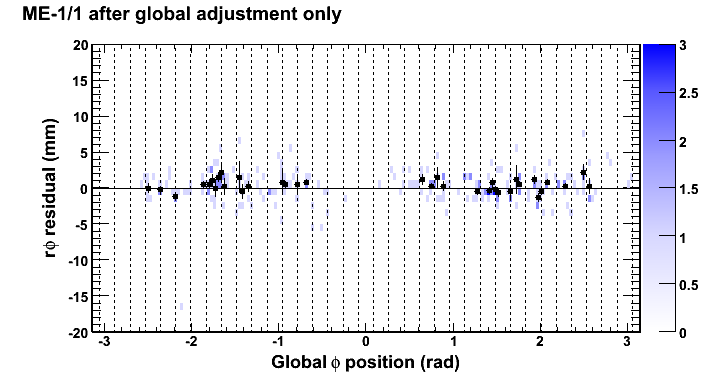
\includegraphics[width=0.5\linewidth]{ringmapplots_3dof/before_CSCvsphi_mem11_x.png} 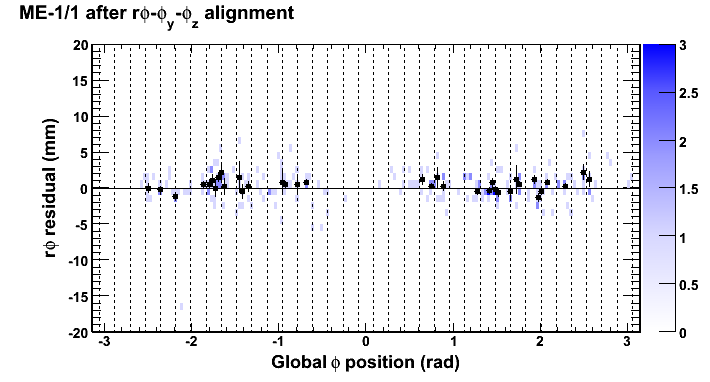
\includegraphics[width=0.5\linewidth]{ringmapplots_3dof/after_CSCvsphi_mem11_x.png}

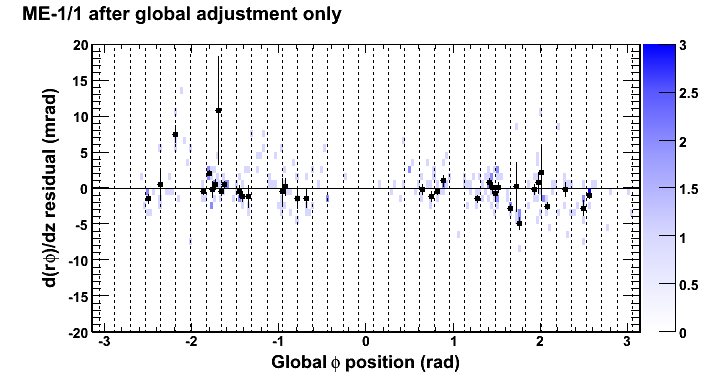
\includegraphics[width=0.5\linewidth]{ringmapplots_3dof/before_CSCvsphi_mem11_dxdz.png} 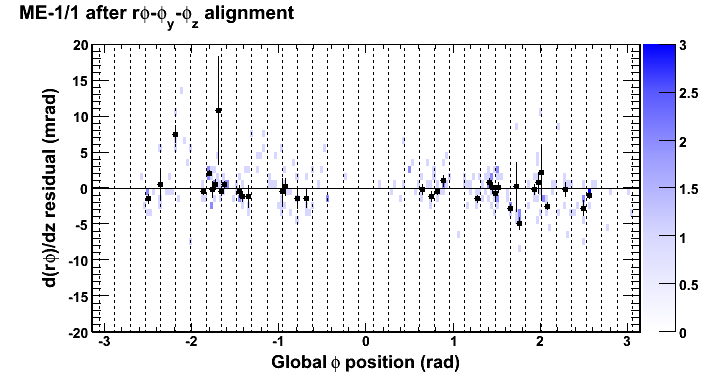
\includegraphics[width=0.5\linewidth]{ringmapplots_3dof/after_CSCvsphi_mem11_dxdz.png}
\end{frame}

\begin{frame}
\frametitle{Map plots}
\framesubtitle{before (left) and after (right) individual chamber alignment}
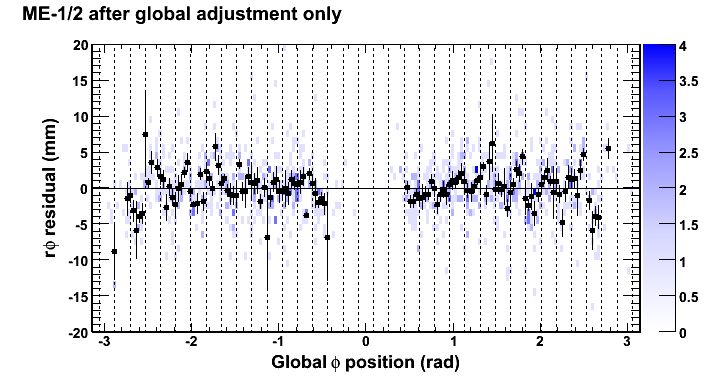
\includegraphics[width=0.5\linewidth]{ringmapplots_3dof/before_CSCvsphi_mem12_x.png} 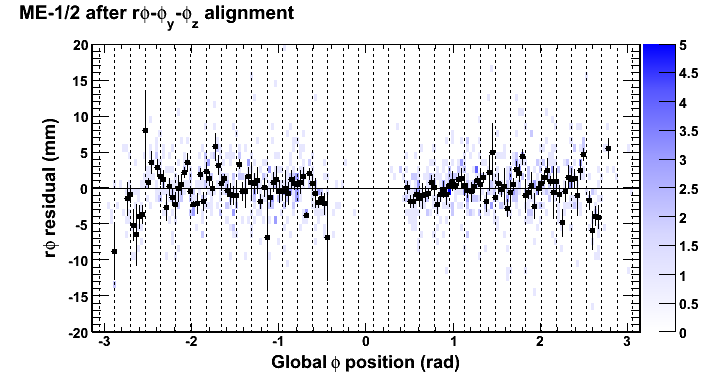
\includegraphics[width=0.5\linewidth]{ringmapplots_3dof/after_CSCvsphi_mem12_x.png}

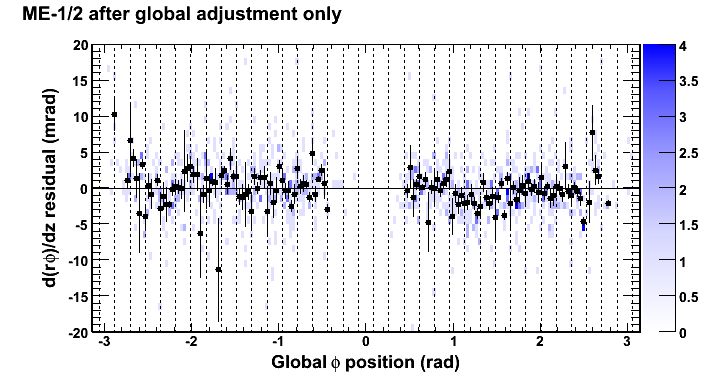
\includegraphics[width=0.5\linewidth]{ringmapplots_3dof/before_CSCvsphi_mem12_dxdz.png} 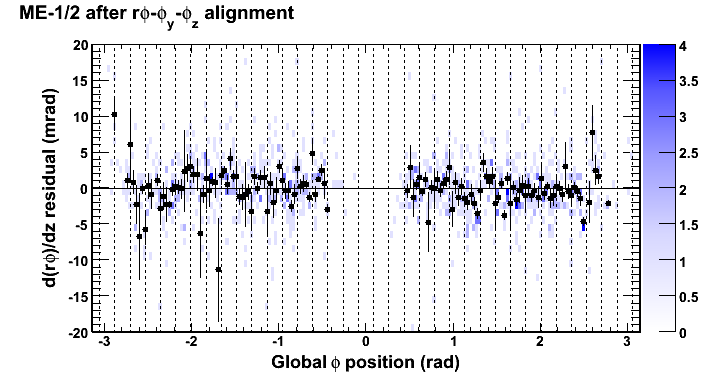
\includegraphics[width=0.5\linewidth]{ringmapplots_3dof/after_CSCvsphi_mem12_dxdz.png}
\end{frame}

\begin{frame}
\frametitle{Map plots}
\framesubtitle{before (left) and after (right) individual chamber alignment}
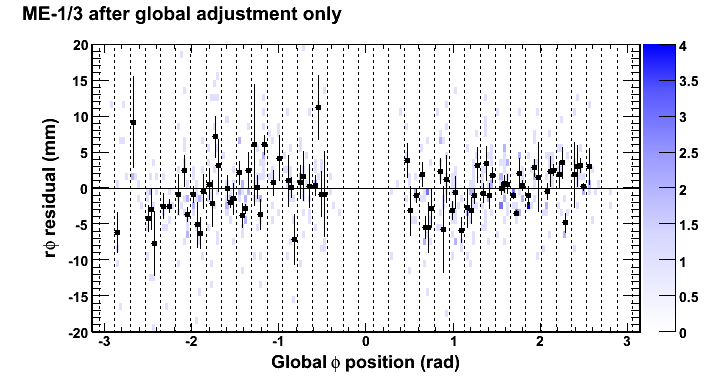
\includegraphics[width=0.5\linewidth]{ringmapplots_3dof/before_CSCvsphi_mem13_x.png} 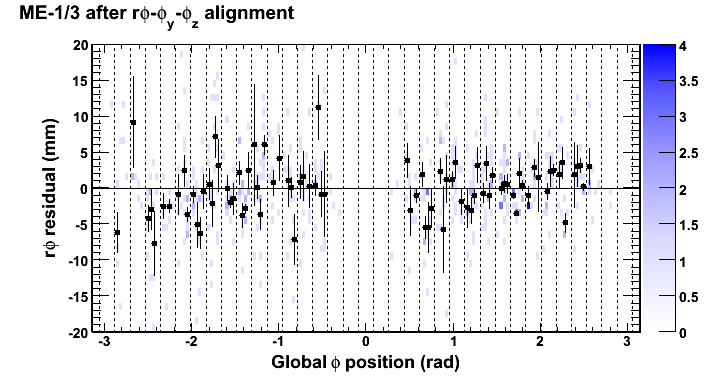
\includegraphics[width=0.5\linewidth]{ringmapplots_3dof/after_CSCvsphi_mem13_x.png}

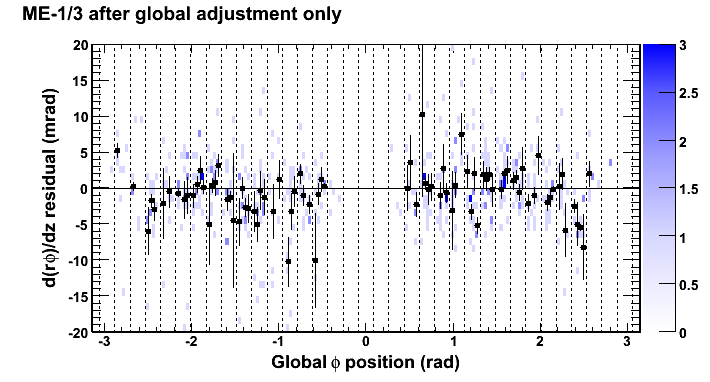
\includegraphics[width=0.5\linewidth]{ringmapplots_3dof/before_CSCvsphi_mem13_dxdz.png} 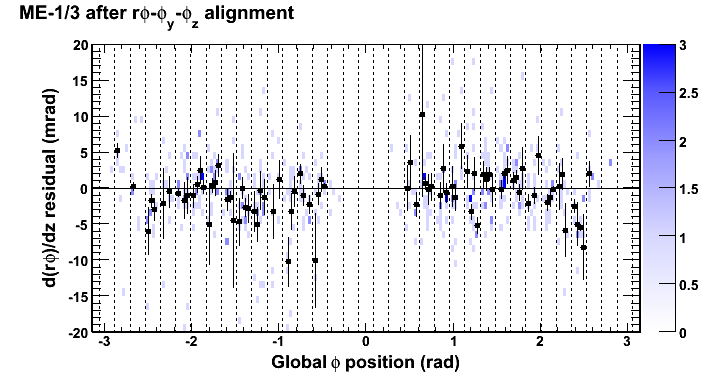
\includegraphics[width=0.5\linewidth]{ringmapplots_3dof/after_CSCvsphi_mem13_dxdz.png}
\end{frame}

\begin{frame}
\frametitle{Map plots}
\framesubtitle{before (left) and after (right) individual chamber alignment}
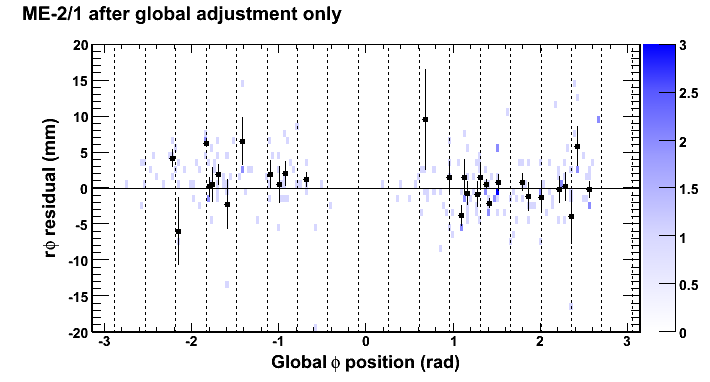
\includegraphics[width=0.5\linewidth]{ringmapplots_3dof/before_CSCvsphi_mem21_x.png} 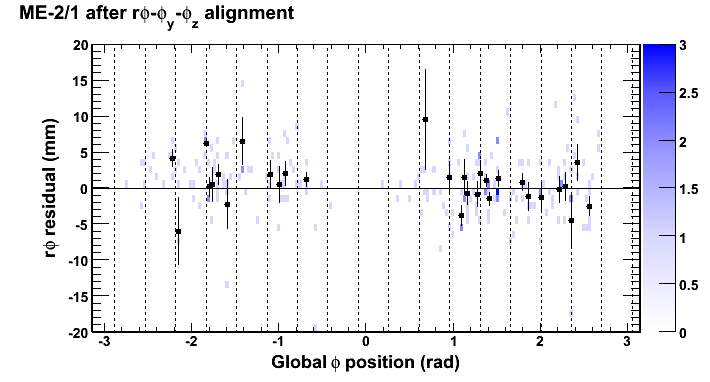
\includegraphics[width=0.5\linewidth]{ringmapplots_3dof/after_CSCvsphi_mem21_x.png}

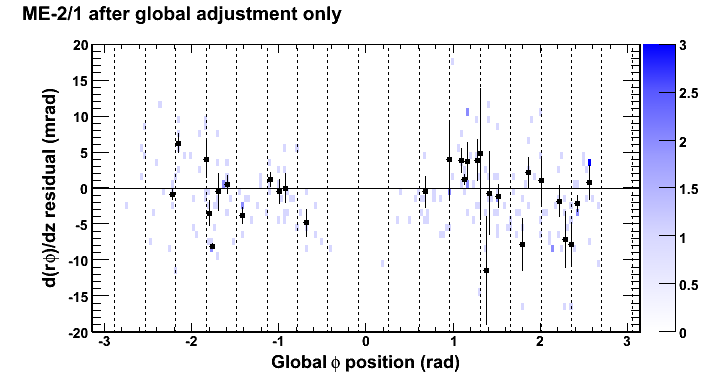
\includegraphics[width=0.5\linewidth]{ringmapplots_3dof/before_CSCvsphi_mem21_dxdz.png} 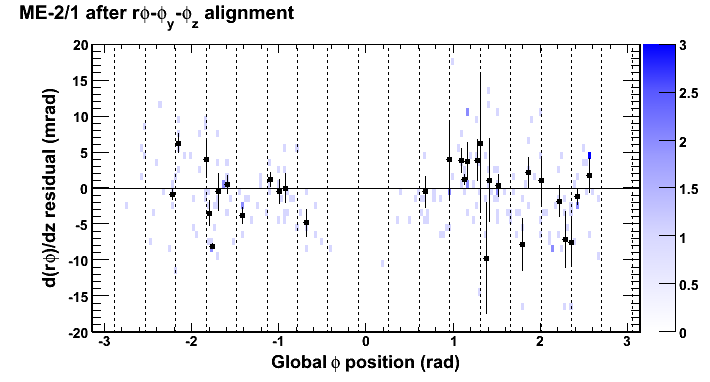
\includegraphics[width=0.5\linewidth]{ringmapplots_3dof/after_CSCvsphi_mem21_dxdz.png}
\end{frame}

\begin{frame}
\frametitle{Map plots}
\framesubtitle{before (left) and after (right) individual chamber alignment}
\includegraphics[width=0.5\linewidth]{ringmapplots_3dof/before_CSCvsphi_mem22_x.png} \includegraphics[width=0.5\linewidth]{ringmapplots_3dof/after_CSCvsphi_mem22_x.png}

\includegraphics[width=0.5\linewidth]{ringmapplots_3dof/before_CSCvsphi_mem22_dxdz.png} \includegraphics[width=0.5\linewidth]{ringmapplots_3dof/after_CSCvsphi_mem22_dxdz.png}
\end{frame}

\begin{frame}
\frametitle{Map plots}
\framesubtitle{before (left) and after (right) individual chamber alignment}
\includegraphics[width=0.5\linewidth]{ringmapplots_3dof/before_CSCvsphi_mem31_x.png} \includegraphics[width=0.5\linewidth]{ringmapplots_3dof/after_CSCvsphi_mem31_x.png}

\includegraphics[width=0.5\linewidth]{ringmapplots_3dof/before_CSCvsphi_mem31_dxdz.png} \includegraphics[width=0.5\linewidth]{ringmapplots_3dof/after_CSCvsphi_mem31_dxdz.png}
\end{frame}

\begin{frame}
\frametitle{Map plots}
\framesubtitle{before (left) and after (right) individual chamber alignment}
\includegraphics[width=0.5\linewidth]{ringmapplots_3dof/before_CSCvsphi_mem32_x.png} \includegraphics[width=0.5\linewidth]{ringmapplots_3dof/after_CSCvsphi_mem32_x.png}

\includegraphics[width=0.5\linewidth]{ringmapplots_3dof/before_CSCvsphi_mem32_dxdz.png} \includegraphics[width=0.5\linewidth]{ringmapplots_3dof/after_CSCvsphi_mem32_dxdz.png}
\end{frame}

\begin{frame}
\frametitle{Map plots}
\framesubtitle{before (left) and after (right) individual chamber alignment}
\includegraphics[width=0.5\linewidth]{ringmapplots_3dof/before_CSCvsphi_mem41_x.png} \includegraphics[width=0.5\linewidth]{ringmapplots_3dof/after_CSCvsphi_mem41_x.png}

\includegraphics[width=0.5\linewidth]{ringmapplots_3dof/before_CSCvsphi_mem41_dxdz.png} \includegraphics[width=0.5\linewidth]{ringmapplots_3dof/after_CSCvsphi_mem41_dxdz.png}
\end{frame}

\begin{frame}
\frametitle{Map plots}
\framesubtitle{before (left) and after (right) individual chamber alignment}
\includegraphics[width=0.5\linewidth]{ringmapplots_3dof/before_CSCvsphi_mep11_x.png} \includegraphics[width=0.5\linewidth]{ringmapplots_3dof/after_CSCvsphi_mep11_x.png}

\includegraphics[width=0.5\linewidth]{ringmapplots_3dof/before_CSCvsphi_mep11_dxdz.png} \includegraphics[width=0.5\linewidth]{ringmapplots_3dof/after_CSCvsphi_mep11_dxdz.png}
\end{frame}

\begin{frame}
\frametitle{Map plots}
\framesubtitle{before (left) and after (right) individual chamber alignment}
\includegraphics[width=0.5\linewidth]{ringmapplots_3dof/before_CSCvsphi_mep12_x.png} \includegraphics[width=0.5\linewidth]{ringmapplots_3dof/after_CSCvsphi_mep12_x.png}

\includegraphics[width=0.5\linewidth]{ringmapplots_3dof/before_CSCvsphi_mep12_dxdz.png} \includegraphics[width=0.5\linewidth]{ringmapplots_3dof/after_CSCvsphi_mep12_dxdz.png}
\end{frame}

\begin{frame}
\frametitle{Map plots}
\framesubtitle{before (left) and after (right) individual chamber alignment}
\includegraphics[width=0.5\linewidth]{ringmapplots_3dof/before_CSCvsphi_mep13_x.png} \includegraphics[width=0.5\linewidth]{ringmapplots_3dof/after_CSCvsphi_mep13_x.png}

\includegraphics[width=0.5\linewidth]{ringmapplots_3dof/before_CSCvsphi_mep13_dxdz.png} \includegraphics[width=0.5\linewidth]{ringmapplots_3dof/after_CSCvsphi_mep13_dxdz.png}
\end{frame}

\begin{frame}
\frametitle{Map plots}
\framesubtitle{before (left) and after (right) individual chamber alignment}
\includegraphics[width=0.5\linewidth]{ringmapplots_3dof/before_CSCvsphi_mep21_x.png} \includegraphics[width=0.5\linewidth]{ringmapplots_3dof/after_CSCvsphi_mep21_x.png}

\includegraphics[width=0.5\linewidth]{ringmapplots_3dof/before_CSCvsphi_mep21_dxdz.png} \includegraphics[width=0.5\linewidth]{ringmapplots_3dof/after_CSCvsphi_mep21_dxdz.png}
\end{frame}

\begin{frame}
\frametitle{Map plots}
\framesubtitle{before (left) and after (right) individual chamber alignment}
\includegraphics[width=0.5\linewidth]{ringmapplots_3dof/before_CSCvsphi_mep22_x.png} \includegraphics[width=0.5\linewidth]{ringmapplots_3dof/after_CSCvsphi_mep22_x.png}

\includegraphics[width=0.5\linewidth]{ringmapplots_3dof/before_CSCvsphi_mep22_dxdz.png} \includegraphics[width=0.5\linewidth]{ringmapplots_3dof/after_CSCvsphi_mep22_dxdz.png}
\end{frame}

\begin{frame}
\frametitle{Map plots}
\framesubtitle{before (left) and after (right) individual chamber alignment}
\includegraphics[width=0.5\linewidth]{ringmapplots_3dof/before_CSCvsphi_mep31_x.png} \includegraphics[width=0.5\linewidth]{ringmapplots_3dof/after_CSCvsphi_mep31_x.png}

\includegraphics[width=0.5\linewidth]{ringmapplots_3dof/before_CSCvsphi_mep31_dxdz.png} \includegraphics[width=0.5\linewidth]{ringmapplots_3dof/after_CSCvsphi_mep31_dxdz.png}
\end{frame}

\begin{frame}
\frametitle{Map plots}
\framesubtitle{before (left) and after (right) individual chamber alignment}
\includegraphics[width=0.5\linewidth]{ringmapplots_3dof/before_CSCvsphi_mep32_x.png} \includegraphics[width=0.5\linewidth]{ringmapplots_3dof/after_CSCvsphi_mep32_x.png}

\includegraphics[width=0.5\linewidth]{ringmapplots_3dof/before_CSCvsphi_mep32_dxdz.png} \includegraphics[width=0.5\linewidth]{ringmapplots_3dof/after_CSCvsphi_mep32_dxdz.png}
\end{frame}

\begin{frame}
\frametitle{Map plots}
\framesubtitle{before (left) and after (right) individual chamber alignment}
\includegraphics[width=0.5\linewidth]{ringmapplots_3dof/before_CSCvsphi_mep41_x.png} \includegraphics[width=0.5\linewidth]{ringmapplots_3dof/after_CSCvsphi_mep41_x.png}

\includegraphics[width=0.5\linewidth]{ringmapplots_3dof/before_CSCvsphi_mep41_dxdz.png} \includegraphics[width=0.5\linewidth]{ringmapplots_3dof/after_CSCvsphi_mep41_dxdz.png}
\end{frame}

\begin{frame}
\frametitle{Map plots}
\framesubtitle{before (left) and after (right) individual chamber alignment}
\includegraphics[width=0.5\linewidth]{ringmapplots_3dof/before_CSCvsr_mem1ch01_x.png} \includegraphics[width=0.5\linewidth]{ringmapplots_3dof/after_CSCvsr_mem1ch01_x.png}

\includegraphics[width=0.5\linewidth]{ringmapplots_3dof/before_CSCvsr_mem1ch01_dxdz.png} \includegraphics[width=0.5\linewidth]{ringmapplots_3dof/after_CSCvsr_mem1ch01_dxdz.png}
\end{frame}

\begin{frame}
\frametitle{Map plots}
\framesubtitle{before (left) and after (right) individual chamber alignment}
\includegraphics[width=0.5\linewidth]{ringmapplots_3dof/before_CSCvsr_mem1ch02_x.png} \includegraphics[width=0.5\linewidth]{ringmapplots_3dof/after_CSCvsr_mem1ch02_x.png}

\includegraphics[width=0.5\linewidth]{ringmapplots_3dof/before_CSCvsr_mem1ch02_dxdz.png} \includegraphics[width=0.5\linewidth]{ringmapplots_3dof/after_CSCvsr_mem1ch02_dxdz.png}
\end{frame}

\begin{frame}
\frametitle{Map plots}
\framesubtitle{before (left) and after (right) individual chamber alignment}
\includegraphics[width=0.5\linewidth]{ringmapplots_3dof/before_CSCvsr_mem1ch03_x.png} \includegraphics[width=0.5\linewidth]{ringmapplots_3dof/after_CSCvsr_mem1ch03_x.png}

\includegraphics[width=0.5\linewidth]{ringmapplots_3dof/before_CSCvsr_mem1ch03_dxdz.png} \includegraphics[width=0.5\linewidth]{ringmapplots_3dof/after_CSCvsr_mem1ch03_dxdz.png}
\end{frame}

\begin{frame}
\frametitle{Map plots}
\framesubtitle{before (left) and after (right) individual chamber alignment}
\includegraphics[width=0.5\linewidth]{ringmapplots_3dof/before_CSCvsr_mem1ch04_x.png} \includegraphics[width=0.5\linewidth]{ringmapplots_3dof/after_CSCvsr_mem1ch04_x.png}

\includegraphics[width=0.5\linewidth]{ringmapplots_3dof/before_CSCvsr_mem1ch04_dxdz.png} \includegraphics[width=0.5\linewidth]{ringmapplots_3dof/after_CSCvsr_mem1ch04_dxdz.png}
\end{frame}

\begin{frame}
\frametitle{Map plots}
\framesubtitle{before (left) and after (right) individual chamber alignment}
\includegraphics[width=0.5\linewidth]{ringmapplots_3dof/before_CSCvsr_mem1ch05_x.png} \includegraphics[width=0.5\linewidth]{ringmapplots_3dof/after_CSCvsr_mem1ch05_x.png}

\includegraphics[width=0.5\linewidth]{ringmapplots_3dof/before_CSCvsr_mem1ch05_dxdz.png} \includegraphics[width=0.5\linewidth]{ringmapplots_3dof/after_CSCvsr_mem1ch05_dxdz.png}
\end{frame}

\begin{frame}
\frametitle{Map plots}
\framesubtitle{before (left) and after (right) individual chamber alignment}
\includegraphics[width=0.5\linewidth]{ringmapplots_3dof/before_CSCvsr_mem1ch06_x.png} \includegraphics[width=0.5\linewidth]{ringmapplots_3dof/after_CSCvsr_mem1ch06_x.png}

\includegraphics[width=0.5\linewidth]{ringmapplots_3dof/before_CSCvsr_mem1ch06_dxdz.png} \includegraphics[width=0.5\linewidth]{ringmapplots_3dof/after_CSCvsr_mem1ch06_dxdz.png}
\end{frame}

\begin{frame}
\frametitle{Map plots}
\framesubtitle{before (left) and after (right) individual chamber alignment}
\includegraphics[width=0.5\linewidth]{ringmapplots_3dof/before_CSCvsr_mem1ch07_x.png} \includegraphics[width=0.5\linewidth]{ringmapplots_3dof/after_CSCvsr_mem1ch07_x.png}

\includegraphics[width=0.5\linewidth]{ringmapplots_3dof/before_CSCvsr_mem1ch07_dxdz.png} \includegraphics[width=0.5\linewidth]{ringmapplots_3dof/after_CSCvsr_mem1ch07_dxdz.png}
\end{frame}

\begin{frame}
\frametitle{Map plots}
\framesubtitle{before (left) and after (right) individual chamber alignment}
\includegraphics[width=0.5\linewidth]{ringmapplots_3dof/before_CSCvsr_mem1ch08_x.png} \includegraphics[width=0.5\linewidth]{ringmapplots_3dof/after_CSCvsr_mem1ch08_x.png}

\includegraphics[width=0.5\linewidth]{ringmapplots_3dof/before_CSCvsr_mem1ch08_dxdz.png} \includegraphics[width=0.5\linewidth]{ringmapplots_3dof/after_CSCvsr_mem1ch08_dxdz.png}
\end{frame}

\begin{frame}
\frametitle{Map plots}
\framesubtitle{before (left) and after (right) individual chamber alignment}
\includegraphics[width=0.5\linewidth]{ringmapplots_3dof/before_CSCvsr_mem1ch09_x.png} \includegraphics[width=0.5\linewidth]{ringmapplots_3dof/after_CSCvsr_mem1ch09_x.png}

\includegraphics[width=0.5\linewidth]{ringmapplots_3dof/before_CSCvsr_mem1ch09_dxdz.png} \includegraphics[width=0.5\linewidth]{ringmapplots_3dof/after_CSCvsr_mem1ch09_dxdz.png}
\end{frame}

\begin{frame}
\frametitle{Map plots}
\framesubtitle{before (left) and after (right) individual chamber alignment}
\includegraphics[width=0.5\linewidth]{ringmapplots_3dof/before_CSCvsr_mem1ch10_x.png} \includegraphics[width=0.5\linewidth]{ringmapplots_3dof/after_CSCvsr_mem1ch10_x.png}

\includegraphics[width=0.5\linewidth]{ringmapplots_3dof/before_CSCvsr_mem1ch10_dxdz.png} \includegraphics[width=0.5\linewidth]{ringmapplots_3dof/after_CSCvsr_mem1ch10_dxdz.png}
\end{frame}

\begin{frame}
\frametitle{Map plots}
\framesubtitle{before (left) and after (right) individual chamber alignment}
\includegraphics[width=0.5\linewidth]{ringmapplots_3dof/before_CSCvsr_mem1ch11_x.png} \includegraphics[width=0.5\linewidth]{ringmapplots_3dof/after_CSCvsr_mem1ch11_x.png}

\includegraphics[width=0.5\linewidth]{ringmapplots_3dof/before_CSCvsr_mem1ch11_dxdz.png} \includegraphics[width=0.5\linewidth]{ringmapplots_3dof/after_CSCvsr_mem1ch11_dxdz.png}
\end{frame}

\begin{frame}
\frametitle{Map plots}
\framesubtitle{before (left) and after (right) individual chamber alignment}
\includegraphics[width=0.5\linewidth]{ringmapplots_3dof/before_CSCvsr_mem1ch12_x.png} \includegraphics[width=0.5\linewidth]{ringmapplots_3dof/after_CSCvsr_mem1ch12_x.png}

\includegraphics[width=0.5\linewidth]{ringmapplots_3dof/before_CSCvsr_mem1ch12_dxdz.png} \includegraphics[width=0.5\linewidth]{ringmapplots_3dof/after_CSCvsr_mem1ch12_dxdz.png}
\end{frame}

\begin{frame}
\frametitle{Map plots}
\framesubtitle{before (left) and after (right) individual chamber alignment}
\includegraphics[width=0.5\linewidth]{ringmapplots_3dof/before_CSCvsr_mem1ch13_x.png} \includegraphics[width=0.5\linewidth]{ringmapplots_3dof/after_CSCvsr_mem1ch13_x.png}

\includegraphics[width=0.5\linewidth]{ringmapplots_3dof/before_CSCvsr_mem1ch13_dxdz.png} \includegraphics[width=0.5\linewidth]{ringmapplots_3dof/after_CSCvsr_mem1ch13_dxdz.png}
\end{frame}

\begin{frame}
\frametitle{Map plots}
\framesubtitle{before (left) and after (right) individual chamber alignment}
\includegraphics[width=0.5\linewidth]{ringmapplots_3dof/before_CSCvsr_mem1ch14_x.png} \includegraphics[width=0.5\linewidth]{ringmapplots_3dof/after_CSCvsr_mem1ch14_x.png}

\includegraphics[width=0.5\linewidth]{ringmapplots_3dof/before_CSCvsr_mem1ch14_dxdz.png} \includegraphics[width=0.5\linewidth]{ringmapplots_3dof/after_CSCvsr_mem1ch14_dxdz.png}
\end{frame}

\begin{frame}
\frametitle{Map plots}
\framesubtitle{before (left) and after (right) individual chamber alignment}
\includegraphics[width=0.5\linewidth]{ringmapplots_3dof/before_CSCvsr_mem1ch15_x.png} \includegraphics[width=0.5\linewidth]{ringmapplots_3dof/after_CSCvsr_mem1ch15_x.png}

\includegraphics[width=0.5\linewidth]{ringmapplots_3dof/before_CSCvsr_mem1ch15_dxdz.png} \includegraphics[width=0.5\linewidth]{ringmapplots_3dof/after_CSCvsr_mem1ch15_dxdz.png}
\end{frame}

\begin{frame}
\frametitle{Map plots}
\framesubtitle{before (left) and after (right) individual chamber alignment}
\includegraphics[width=0.5\linewidth]{ringmapplots_3dof/before_CSCvsr_mem1ch16_x.png} \includegraphics[width=0.5\linewidth]{ringmapplots_3dof/after_CSCvsr_mem1ch16_x.png}

\includegraphics[width=0.5\linewidth]{ringmapplots_3dof/before_CSCvsr_mem1ch16_dxdz.png} \includegraphics[width=0.5\linewidth]{ringmapplots_3dof/after_CSCvsr_mem1ch16_dxdz.png}
\end{frame}

\begin{frame}
\frametitle{Map plots}
\framesubtitle{before (left) and after (right) individual chamber alignment}
\includegraphics[width=0.5\linewidth]{ringmapplots_3dof/before_CSCvsr_mem1ch17_x.png} \includegraphics[width=0.5\linewidth]{ringmapplots_3dof/after_CSCvsr_mem1ch17_x.png}

\includegraphics[width=0.5\linewidth]{ringmapplots_3dof/before_CSCvsr_mem1ch17_dxdz.png} \includegraphics[width=0.5\linewidth]{ringmapplots_3dof/after_CSCvsr_mem1ch17_dxdz.png}
\end{frame}

\begin{frame}
\frametitle{Map plots}
\framesubtitle{before (left) and after (right) individual chamber alignment}
\includegraphics[width=0.5\linewidth]{ringmapplots_3dof/before_CSCvsr_mem1ch18_x.png} \includegraphics[width=0.5\linewidth]{ringmapplots_3dof/after_CSCvsr_mem1ch18_x.png}

\includegraphics[width=0.5\linewidth]{ringmapplots_3dof/before_CSCvsr_mem1ch18_dxdz.png} \includegraphics[width=0.5\linewidth]{ringmapplots_3dof/after_CSCvsr_mem1ch18_dxdz.png}
\end{frame}

\begin{frame}
\frametitle{Map plots}
\framesubtitle{before (left) and after (right) individual chamber alignment}
\includegraphics[width=0.5\linewidth]{ringmapplots_3dof/before_CSCvsr_mem1ch19_x.png} \includegraphics[width=0.5\linewidth]{ringmapplots_3dof/after_CSCvsr_mem1ch19_x.png}

\includegraphics[width=0.5\linewidth]{ringmapplots_3dof/before_CSCvsr_mem1ch19_dxdz.png} \includegraphics[width=0.5\linewidth]{ringmapplots_3dof/after_CSCvsr_mem1ch19_dxdz.png}
\end{frame}

\begin{frame}
\frametitle{Map plots}
\framesubtitle{before (left) and after (right) individual chamber alignment}
\includegraphics[width=0.5\linewidth]{ringmapplots_3dof/before_CSCvsr_mem1ch20_x.png} \includegraphics[width=0.5\linewidth]{ringmapplots_3dof/after_CSCvsr_mem1ch20_x.png}

\includegraphics[width=0.5\linewidth]{ringmapplots_3dof/before_CSCvsr_mem1ch20_dxdz.png} \includegraphics[width=0.5\linewidth]{ringmapplots_3dof/after_CSCvsr_mem1ch20_dxdz.png}
\end{frame}

\begin{frame}
\frametitle{Map plots}
\framesubtitle{before (left) and after (right) individual chamber alignment}
\includegraphics[width=0.5\linewidth]{ringmapplots_3dof/before_CSCvsr_mem1ch21_x.png} \includegraphics[width=0.5\linewidth]{ringmapplots_3dof/after_CSCvsr_mem1ch21_x.png}

\includegraphics[width=0.5\linewidth]{ringmapplots_3dof/before_CSCvsr_mem1ch21_dxdz.png} \includegraphics[width=0.5\linewidth]{ringmapplots_3dof/after_CSCvsr_mem1ch21_dxdz.png}
\end{frame}

\begin{frame}
\frametitle{Map plots}
\framesubtitle{before (left) and after (right) individual chamber alignment}
\includegraphics[width=0.5\linewidth]{ringmapplots_3dof/before_CSCvsr_mem1ch22_x.png} \includegraphics[width=0.5\linewidth]{ringmapplots_3dof/after_CSCvsr_mem1ch22_x.png}

\includegraphics[width=0.5\linewidth]{ringmapplots_3dof/before_CSCvsr_mem1ch22_dxdz.png} \includegraphics[width=0.5\linewidth]{ringmapplots_3dof/after_CSCvsr_mem1ch22_dxdz.png}
\end{frame}

\begin{frame}
\frametitle{Map plots}
\framesubtitle{before (left) and after (right) individual chamber alignment}
\includegraphics[width=0.5\linewidth]{ringmapplots_3dof/before_CSCvsr_mem1ch23_x.png} \includegraphics[width=0.5\linewidth]{ringmapplots_3dof/after_CSCvsr_mem1ch23_x.png}

\includegraphics[width=0.5\linewidth]{ringmapplots_3dof/before_CSCvsr_mem1ch23_dxdz.png} \includegraphics[width=0.5\linewidth]{ringmapplots_3dof/after_CSCvsr_mem1ch23_dxdz.png}
\end{frame}

\begin{frame}
\frametitle{Map plots}
\framesubtitle{before (left) and after (right) individual chamber alignment}
\includegraphics[width=0.5\linewidth]{ringmapplots_3dof/before_CSCvsr_mem1ch24_x.png} \includegraphics[width=0.5\linewidth]{ringmapplots_3dof/after_CSCvsr_mem1ch24_x.png}

\includegraphics[width=0.5\linewidth]{ringmapplots_3dof/before_CSCvsr_mem1ch24_dxdz.png} \includegraphics[width=0.5\linewidth]{ringmapplots_3dof/after_CSCvsr_mem1ch24_dxdz.png}
\end{frame}

\begin{frame}
\frametitle{Map plots}
\framesubtitle{before (left) and after (right) individual chamber alignment}
\includegraphics[width=0.5\linewidth]{ringmapplots_3dof/before_CSCvsr_mem1ch25_x.png} \includegraphics[width=0.5\linewidth]{ringmapplots_3dof/after_CSCvsr_mem1ch25_x.png}

\includegraphics[width=0.5\linewidth]{ringmapplots_3dof/before_CSCvsr_mem1ch25_dxdz.png} \includegraphics[width=0.5\linewidth]{ringmapplots_3dof/after_CSCvsr_mem1ch25_dxdz.png}
\end{frame}

\begin{frame}
\frametitle{Map plots}
\framesubtitle{before (left) and after (right) individual chamber alignment}
\includegraphics[width=0.5\linewidth]{ringmapplots_3dof/before_CSCvsr_mem1ch26_x.png} \includegraphics[width=0.5\linewidth]{ringmapplots_3dof/after_CSCvsr_mem1ch26_x.png}

\includegraphics[width=0.5\linewidth]{ringmapplots_3dof/before_CSCvsr_mem1ch26_dxdz.png} \includegraphics[width=0.5\linewidth]{ringmapplots_3dof/after_CSCvsr_mem1ch26_dxdz.png}
\end{frame}

\begin{frame}
\frametitle{Map plots}
\framesubtitle{before (left) and after (right) individual chamber alignment}
\includegraphics[width=0.5\linewidth]{ringmapplots_3dof/before_CSCvsr_mem1ch27_x.png} \includegraphics[width=0.5\linewidth]{ringmapplots_3dof/after_CSCvsr_mem1ch27_x.png}

\includegraphics[width=0.5\linewidth]{ringmapplots_3dof/before_CSCvsr_mem1ch27_dxdz.png} \includegraphics[width=0.5\linewidth]{ringmapplots_3dof/after_CSCvsr_mem1ch27_dxdz.png}
\end{frame}

\begin{frame}
\frametitle{Map plots}
\framesubtitle{before (left) and after (right) individual chamber alignment}
\includegraphics[width=0.5\linewidth]{ringmapplots_3dof/before_CSCvsr_mem1ch28_x.png} \includegraphics[width=0.5\linewidth]{ringmapplots_3dof/after_CSCvsr_mem1ch28_x.png}

\includegraphics[width=0.5\linewidth]{ringmapplots_3dof/before_CSCvsr_mem1ch28_dxdz.png} \includegraphics[width=0.5\linewidth]{ringmapplots_3dof/after_CSCvsr_mem1ch28_dxdz.png}
\end{frame}

\begin{frame}
\frametitle{Map plots}
\framesubtitle{before (left) and after (right) individual chamber alignment}
\includegraphics[width=0.5\linewidth]{ringmapplots_3dof/before_CSCvsr_mem1ch29_x.png} \includegraphics[width=0.5\linewidth]{ringmapplots_3dof/after_CSCvsr_mem1ch29_x.png}

\includegraphics[width=0.5\linewidth]{ringmapplots_3dof/before_CSCvsr_mem1ch29_dxdz.png} \includegraphics[width=0.5\linewidth]{ringmapplots_3dof/after_CSCvsr_mem1ch29_dxdz.png}
\end{frame}

\begin{frame}
\frametitle{Map plots}
\framesubtitle{before (left) and after (right) individual chamber alignment}
\includegraphics[width=0.5\linewidth]{ringmapplots_3dof/before_CSCvsr_mem1ch30_x.png} \includegraphics[width=0.5\linewidth]{ringmapplots_3dof/after_CSCvsr_mem1ch30_x.png}

\includegraphics[width=0.5\linewidth]{ringmapplots_3dof/before_CSCvsr_mem1ch30_dxdz.png} \includegraphics[width=0.5\linewidth]{ringmapplots_3dof/after_CSCvsr_mem1ch30_dxdz.png}
\end{frame}

\begin{frame}
\frametitle{Map plots}
\framesubtitle{before (left) and after (right) individual chamber alignment}
\includegraphics[width=0.5\linewidth]{ringmapplots_3dof/before_CSCvsr_mem1ch31_x.png} \includegraphics[width=0.5\linewidth]{ringmapplots_3dof/after_CSCvsr_mem1ch31_x.png}

\includegraphics[width=0.5\linewidth]{ringmapplots_3dof/before_CSCvsr_mem1ch31_dxdz.png} \includegraphics[width=0.5\linewidth]{ringmapplots_3dof/after_CSCvsr_mem1ch31_dxdz.png}
\end{frame}

\begin{frame}
\frametitle{Map plots}
\framesubtitle{before (left) and after (right) individual chamber alignment}
\includegraphics[width=0.5\linewidth]{ringmapplots_3dof/before_CSCvsr_mem1ch32_x.png} \includegraphics[width=0.5\linewidth]{ringmapplots_3dof/after_CSCvsr_mem1ch32_x.png}

\includegraphics[width=0.5\linewidth]{ringmapplots_3dof/before_CSCvsr_mem1ch32_dxdz.png} \includegraphics[width=0.5\linewidth]{ringmapplots_3dof/after_CSCvsr_mem1ch32_dxdz.png}
\end{frame}

\begin{frame}
\frametitle{Map plots}
\framesubtitle{before (left) and after (right) individual chamber alignment}
\includegraphics[width=0.5\linewidth]{ringmapplots_3dof/before_CSCvsr_mem1ch33_x.png} \includegraphics[width=0.5\linewidth]{ringmapplots_3dof/after_CSCvsr_mem1ch33_x.png}

\includegraphics[width=0.5\linewidth]{ringmapplots_3dof/before_CSCvsr_mem1ch33_dxdz.png} \includegraphics[width=0.5\linewidth]{ringmapplots_3dof/after_CSCvsr_mem1ch33_dxdz.png}
\end{frame}

\begin{frame}
\frametitle{Map plots}
\framesubtitle{before (left) and after (right) individual chamber alignment}
\includegraphics[width=0.5\linewidth]{ringmapplots_3dof/before_CSCvsr_mem1ch34_x.png} \includegraphics[width=0.5\linewidth]{ringmapplots_3dof/after_CSCvsr_mem1ch34_x.png}

\includegraphics[width=0.5\linewidth]{ringmapplots_3dof/before_CSCvsr_mem1ch34_dxdz.png} \includegraphics[width=0.5\linewidth]{ringmapplots_3dof/after_CSCvsr_mem1ch34_dxdz.png}
\end{frame}

\begin{frame}
\frametitle{Map plots}
\framesubtitle{before (left) and after (right) individual chamber alignment}
\includegraphics[width=0.5\linewidth]{ringmapplots_3dof/before_CSCvsr_mem1ch35_x.png} \includegraphics[width=0.5\linewidth]{ringmapplots_3dof/after_CSCvsr_mem1ch35_x.png}

\includegraphics[width=0.5\linewidth]{ringmapplots_3dof/before_CSCvsr_mem1ch35_dxdz.png} \includegraphics[width=0.5\linewidth]{ringmapplots_3dof/after_CSCvsr_mem1ch35_dxdz.png}
\end{frame}

\begin{frame}
\frametitle{Map plots}
\framesubtitle{before (left) and after (right) individual chamber alignment}
\includegraphics[width=0.5\linewidth]{ringmapplots_3dof/before_CSCvsr_mem1ch36_x.png} \includegraphics[width=0.5\linewidth]{ringmapplots_3dof/after_CSCvsr_mem1ch36_x.png}

\includegraphics[width=0.5\linewidth]{ringmapplots_3dof/before_CSCvsr_mem1ch36_dxdz.png} \includegraphics[width=0.5\linewidth]{ringmapplots_3dof/after_CSCvsr_mem1ch36_dxdz.png}
\end{frame}

\begin{frame}
\frametitle{Map plots}
\framesubtitle{before (left) and after (right) individual chamber alignment}
\includegraphics[width=0.5\linewidth]{ringmapplots_3dof/before_CSCvsr_mem2ch01_x.png} \includegraphics[width=0.5\linewidth]{ringmapplots_3dof/after_CSCvsr_mem2ch01_x.png}

\includegraphics[width=0.5\linewidth]{ringmapplots_3dof/before_CSCvsr_mem2ch01_dxdz.png} \includegraphics[width=0.5\linewidth]{ringmapplots_3dof/after_CSCvsr_mem2ch01_dxdz.png}
\end{frame}

\begin{frame}
\frametitle{Map plots}
\framesubtitle{before (left) and after (right) individual chamber alignment}
\includegraphics[width=0.5\linewidth]{ringmapplots_3dof/before_CSCvsr_mem2ch02_x.png} \includegraphics[width=0.5\linewidth]{ringmapplots_3dof/after_CSCvsr_mem2ch02_x.png}

\includegraphics[width=0.5\linewidth]{ringmapplots_3dof/before_CSCvsr_mem2ch02_dxdz.png} \includegraphics[width=0.5\linewidth]{ringmapplots_3dof/after_CSCvsr_mem2ch02_dxdz.png}
\end{frame}

\begin{frame}
\frametitle{Map plots}
\framesubtitle{before (left) and after (right) individual chamber alignment}
\includegraphics[width=0.5\linewidth]{ringmapplots_3dof/before_CSCvsr_mem2ch03_x.png} \includegraphics[width=0.5\linewidth]{ringmapplots_3dof/after_CSCvsr_mem2ch03_x.png}

\includegraphics[width=0.5\linewidth]{ringmapplots_3dof/before_CSCvsr_mem2ch03_dxdz.png} \includegraphics[width=0.5\linewidth]{ringmapplots_3dof/after_CSCvsr_mem2ch03_dxdz.png}
\end{frame}

\begin{frame}
\frametitle{Map plots}
\framesubtitle{before (left) and after (right) individual chamber alignment}
\includegraphics[width=0.5\linewidth]{ringmapplots_3dof/before_CSCvsr_mem2ch04_x.png} \includegraphics[width=0.5\linewidth]{ringmapplots_3dof/after_CSCvsr_mem2ch04_x.png}

\includegraphics[width=0.5\linewidth]{ringmapplots_3dof/before_CSCvsr_mem2ch04_dxdz.png} \includegraphics[width=0.5\linewidth]{ringmapplots_3dof/after_CSCvsr_mem2ch04_dxdz.png}
\end{frame}

\begin{frame}
\frametitle{Map plots}
\framesubtitle{before (left) and after (right) individual chamber alignment}
\includegraphics[width=0.5\linewidth]{ringmapplots_3dof/before_CSCvsr_mem2ch05_x.png} \includegraphics[width=0.5\linewidth]{ringmapplots_3dof/after_CSCvsr_mem2ch05_x.png}

\includegraphics[width=0.5\linewidth]{ringmapplots_3dof/before_CSCvsr_mem2ch05_dxdz.png} \includegraphics[width=0.5\linewidth]{ringmapplots_3dof/after_CSCvsr_mem2ch05_dxdz.png}
\end{frame}

\begin{frame}
\frametitle{Map plots}
\framesubtitle{before (left) and after (right) individual chamber alignment}
\includegraphics[width=0.5\linewidth]{ringmapplots_3dof/before_CSCvsr_mem2ch06_x.png} \includegraphics[width=0.5\linewidth]{ringmapplots_3dof/after_CSCvsr_mem2ch06_x.png}

\includegraphics[width=0.5\linewidth]{ringmapplots_3dof/before_CSCvsr_mem2ch06_dxdz.png} \includegraphics[width=0.5\linewidth]{ringmapplots_3dof/after_CSCvsr_mem2ch06_dxdz.png}
\end{frame}

\begin{frame}
\frametitle{Map plots}
\framesubtitle{before (left) and after (right) individual chamber alignment}
\includegraphics[width=0.5\linewidth]{ringmapplots_3dof/before_CSCvsr_mem2ch07_x.png} \includegraphics[width=0.5\linewidth]{ringmapplots_3dof/after_CSCvsr_mem2ch07_x.png}

\includegraphics[width=0.5\linewidth]{ringmapplots_3dof/before_CSCvsr_mem2ch07_dxdz.png} \includegraphics[width=0.5\linewidth]{ringmapplots_3dof/after_CSCvsr_mem2ch07_dxdz.png}
\end{frame}

\begin{frame}
\frametitle{Map plots}
\framesubtitle{before (left) and after (right) individual chamber alignment}
\includegraphics[width=0.5\linewidth]{ringmapplots_3dof/before_CSCvsr_mem2ch08_x.png} \includegraphics[width=0.5\linewidth]{ringmapplots_3dof/after_CSCvsr_mem2ch08_x.png}

\includegraphics[width=0.5\linewidth]{ringmapplots_3dof/before_CSCvsr_mem2ch08_dxdz.png} \includegraphics[width=0.5\linewidth]{ringmapplots_3dof/after_CSCvsr_mem2ch08_dxdz.png}
\end{frame}

\begin{frame}
\frametitle{Map plots}
\framesubtitle{before (left) and after (right) individual chamber alignment}
\includegraphics[width=0.5\linewidth]{ringmapplots_3dof/before_CSCvsr_mem2ch09_x.png} \includegraphics[width=0.5\linewidth]{ringmapplots_3dof/after_CSCvsr_mem2ch09_x.png}

\includegraphics[width=0.5\linewidth]{ringmapplots_3dof/before_CSCvsr_mem2ch09_dxdz.png} \includegraphics[width=0.5\linewidth]{ringmapplots_3dof/after_CSCvsr_mem2ch09_dxdz.png}
\end{frame}

\begin{frame}
\frametitle{Map plots}
\framesubtitle{before (left) and after (right) individual chamber alignment}
\includegraphics[width=0.5\linewidth]{ringmapplots_3dof/before_CSCvsr_mem2ch10_x.png} \includegraphics[width=0.5\linewidth]{ringmapplots_3dof/after_CSCvsr_mem2ch10_x.png}

\includegraphics[width=0.5\linewidth]{ringmapplots_3dof/before_CSCvsr_mem2ch10_dxdz.png} \includegraphics[width=0.5\linewidth]{ringmapplots_3dof/after_CSCvsr_mem2ch10_dxdz.png}
\end{frame}

\begin{frame}
\frametitle{Map plots}
\framesubtitle{before (left) and after (right) individual chamber alignment}
\includegraphics[width=0.5\linewidth]{ringmapplots_3dof/before_CSCvsr_mem2ch11_x.png} \includegraphics[width=0.5\linewidth]{ringmapplots_3dof/after_CSCvsr_mem2ch11_x.png}

\includegraphics[width=0.5\linewidth]{ringmapplots_3dof/before_CSCvsr_mem2ch11_dxdz.png} \includegraphics[width=0.5\linewidth]{ringmapplots_3dof/after_CSCvsr_mem2ch11_dxdz.png}
\end{frame}

\begin{frame}
\frametitle{Map plots}
\framesubtitle{before (left) and after (right) individual chamber alignment}
\includegraphics[width=0.5\linewidth]{ringmapplots_3dof/before_CSCvsr_mem2ch12_x.png} \includegraphics[width=0.5\linewidth]{ringmapplots_3dof/after_CSCvsr_mem2ch12_x.png}

\includegraphics[width=0.5\linewidth]{ringmapplots_3dof/before_CSCvsr_mem2ch12_dxdz.png} \includegraphics[width=0.5\linewidth]{ringmapplots_3dof/after_CSCvsr_mem2ch12_dxdz.png}
\end{frame}

\begin{frame}
\frametitle{Map plots}
\framesubtitle{before (left) and after (right) individual chamber alignment}
\includegraphics[width=0.5\linewidth]{ringmapplots_3dof/before_CSCvsr_mem2ch13_x.png} \includegraphics[width=0.5\linewidth]{ringmapplots_3dof/after_CSCvsr_mem2ch13_x.png}

\includegraphics[width=0.5\linewidth]{ringmapplots_3dof/before_CSCvsr_mem2ch13_dxdz.png} \includegraphics[width=0.5\linewidth]{ringmapplots_3dof/after_CSCvsr_mem2ch13_dxdz.png}
\end{frame}

\begin{frame}
\frametitle{Map plots}
\framesubtitle{before (left) and after (right) individual chamber alignment}
\includegraphics[width=0.5\linewidth]{ringmapplots_3dof/before_CSCvsr_mem2ch14_x.png} \includegraphics[width=0.5\linewidth]{ringmapplots_3dof/after_CSCvsr_mem2ch14_x.png}

\includegraphics[width=0.5\linewidth]{ringmapplots_3dof/before_CSCvsr_mem2ch14_dxdz.png} \includegraphics[width=0.5\linewidth]{ringmapplots_3dof/after_CSCvsr_mem2ch14_dxdz.png}
\end{frame}

\begin{frame}
\frametitle{Map plots}
\framesubtitle{before (left) and after (right) individual chamber alignment}
\includegraphics[width=0.5\linewidth]{ringmapplots_3dof/before_CSCvsr_mem2ch15_x.png} \includegraphics[width=0.5\linewidth]{ringmapplots_3dof/after_CSCvsr_mem2ch15_x.png}

\includegraphics[width=0.5\linewidth]{ringmapplots_3dof/before_CSCvsr_mem2ch15_dxdz.png} \includegraphics[width=0.5\linewidth]{ringmapplots_3dof/after_CSCvsr_mem2ch15_dxdz.png}
\end{frame}

\begin{frame}
\frametitle{Map plots}
\framesubtitle{before (left) and after (right) individual chamber alignment}
\includegraphics[width=0.5\linewidth]{ringmapplots_3dof/before_CSCvsr_mem2ch16_x.png} \includegraphics[width=0.5\linewidth]{ringmapplots_3dof/after_CSCvsr_mem2ch16_x.png}

\includegraphics[width=0.5\linewidth]{ringmapplots_3dof/before_CSCvsr_mem2ch16_dxdz.png} \includegraphics[width=0.5\linewidth]{ringmapplots_3dof/after_CSCvsr_mem2ch16_dxdz.png}
\end{frame}

\begin{frame}
\frametitle{Map plots}
\framesubtitle{before (left) and after (right) individual chamber alignment}
\includegraphics[width=0.5\linewidth]{ringmapplots_3dof/before_CSCvsr_mem2ch17_x.png} \includegraphics[width=0.5\linewidth]{ringmapplots_3dof/after_CSCvsr_mem2ch17_x.png}

\includegraphics[width=0.5\linewidth]{ringmapplots_3dof/before_CSCvsr_mem2ch17_dxdz.png} \includegraphics[width=0.5\linewidth]{ringmapplots_3dof/after_CSCvsr_mem2ch17_dxdz.png}
\end{frame}

\begin{frame}
\frametitle{Map plots}
\framesubtitle{before (left) and after (right) individual chamber alignment}
\includegraphics[width=0.5\linewidth]{ringmapplots_3dof/before_CSCvsr_mem2ch18_x.png} \includegraphics[width=0.5\linewidth]{ringmapplots_3dof/after_CSCvsr_mem2ch18_x.png}

\includegraphics[width=0.5\linewidth]{ringmapplots_3dof/before_CSCvsr_mem2ch18_dxdz.png} \includegraphics[width=0.5\linewidth]{ringmapplots_3dof/after_CSCvsr_mem2ch18_dxdz.png}
\end{frame}

\begin{frame}
\frametitle{Map plots}
\framesubtitle{before (left) and after (right) individual chamber alignment}
\includegraphics[width=0.5\linewidth]{ringmapplots_3dof/before_CSCvsr_mem3ch01_x.png} \includegraphics[width=0.5\linewidth]{ringmapplots_3dof/after_CSCvsr_mem3ch01_x.png}

\includegraphics[width=0.5\linewidth]{ringmapplots_3dof/before_CSCvsr_mem3ch01_dxdz.png} \includegraphics[width=0.5\linewidth]{ringmapplots_3dof/after_CSCvsr_mem3ch01_dxdz.png}
\end{frame}

\begin{frame}
\frametitle{Map plots}
\framesubtitle{before (left) and after (right) individual chamber alignment}
\includegraphics[width=0.5\linewidth]{ringmapplots_3dof/before_CSCvsr_mem3ch02_x.png} \includegraphics[width=0.5\linewidth]{ringmapplots_3dof/after_CSCvsr_mem3ch02_x.png}

\includegraphics[width=0.5\linewidth]{ringmapplots_3dof/before_CSCvsr_mem3ch02_dxdz.png} \includegraphics[width=0.5\linewidth]{ringmapplots_3dof/after_CSCvsr_mem3ch02_dxdz.png}
\end{frame}

\begin{frame}
\frametitle{Map plots}
\framesubtitle{before (left) and after (right) individual chamber alignment}
\includegraphics[width=0.5\linewidth]{ringmapplots_3dof/before_CSCvsr_mem3ch03_x.png} \includegraphics[width=0.5\linewidth]{ringmapplots_3dof/after_CSCvsr_mem3ch03_x.png}

\includegraphics[width=0.5\linewidth]{ringmapplots_3dof/before_CSCvsr_mem3ch03_dxdz.png} \includegraphics[width=0.5\linewidth]{ringmapplots_3dof/after_CSCvsr_mem3ch03_dxdz.png}
\end{frame}

\begin{frame}
\frametitle{Map plots}
\framesubtitle{before (left) and after (right) individual chamber alignment}
\includegraphics[width=0.5\linewidth]{ringmapplots_3dof/before_CSCvsr_mem3ch04_x.png} \includegraphics[width=0.5\linewidth]{ringmapplots_3dof/after_CSCvsr_mem3ch04_x.png}

\includegraphics[width=0.5\linewidth]{ringmapplots_3dof/before_CSCvsr_mem3ch04_dxdz.png} \includegraphics[width=0.5\linewidth]{ringmapplots_3dof/after_CSCvsr_mem3ch04_dxdz.png}
\end{frame}

\begin{frame}
\frametitle{Map plots}
\framesubtitle{before (left) and after (right) individual chamber alignment}
\includegraphics[width=0.5\linewidth]{ringmapplots_3dof/before_CSCvsr_mem3ch05_x.png} \includegraphics[width=0.5\linewidth]{ringmapplots_3dof/after_CSCvsr_mem3ch05_x.png}

\includegraphics[width=0.5\linewidth]{ringmapplots_3dof/before_CSCvsr_mem3ch05_dxdz.png} \includegraphics[width=0.5\linewidth]{ringmapplots_3dof/after_CSCvsr_mem3ch05_dxdz.png}
\end{frame}

\begin{frame}
\frametitle{Map plots}
\framesubtitle{before (left) and after (right) individual chamber alignment}
\includegraphics[width=0.5\linewidth]{ringmapplots_3dof/before_CSCvsr_mem3ch06_x.png} \includegraphics[width=0.5\linewidth]{ringmapplots_3dof/after_CSCvsr_mem3ch06_x.png}

\includegraphics[width=0.5\linewidth]{ringmapplots_3dof/before_CSCvsr_mem3ch06_dxdz.png} \includegraphics[width=0.5\linewidth]{ringmapplots_3dof/after_CSCvsr_mem3ch06_dxdz.png}
\end{frame}

\begin{frame}
\frametitle{Map plots}
\framesubtitle{before (left) and after (right) individual chamber alignment}
\includegraphics[width=0.5\linewidth]{ringmapplots_3dof/before_CSCvsr_mem3ch07_x.png} \includegraphics[width=0.5\linewidth]{ringmapplots_3dof/after_CSCvsr_mem3ch07_x.png}

\includegraphics[width=0.5\linewidth]{ringmapplots_3dof/before_CSCvsr_mem3ch07_dxdz.png} \includegraphics[width=0.5\linewidth]{ringmapplots_3dof/after_CSCvsr_mem3ch07_dxdz.png}
\end{frame}

\begin{frame}
\frametitle{Map plots}
\framesubtitle{before (left) and after (right) individual chamber alignment}
\includegraphics[width=0.5\linewidth]{ringmapplots_3dof/before_CSCvsr_mem3ch08_x.png} \includegraphics[width=0.5\linewidth]{ringmapplots_3dof/after_CSCvsr_mem3ch08_x.png}

\includegraphics[width=0.5\linewidth]{ringmapplots_3dof/before_CSCvsr_mem3ch08_dxdz.png} \includegraphics[width=0.5\linewidth]{ringmapplots_3dof/after_CSCvsr_mem3ch08_dxdz.png}
\end{frame}

\begin{frame}
\frametitle{Map plots}
\framesubtitle{before (left) and after (right) individual chamber alignment}
\includegraphics[width=0.5\linewidth]{ringmapplots_3dof/before_CSCvsr_mem3ch09_x.png} \includegraphics[width=0.5\linewidth]{ringmapplots_3dof/after_CSCvsr_mem3ch09_x.png}

\includegraphics[width=0.5\linewidth]{ringmapplots_3dof/before_CSCvsr_mem3ch09_dxdz.png} \includegraphics[width=0.5\linewidth]{ringmapplots_3dof/after_CSCvsr_mem3ch09_dxdz.png}
\end{frame}

\begin{frame}
\frametitle{Map plots}
\framesubtitle{before (left) and after (right) individual chamber alignment}
\includegraphics[width=0.5\linewidth]{ringmapplots_3dof/before_CSCvsr_mem3ch10_x.png} \includegraphics[width=0.5\linewidth]{ringmapplots_3dof/after_CSCvsr_mem3ch10_x.png}

\includegraphics[width=0.5\linewidth]{ringmapplots_3dof/before_CSCvsr_mem3ch10_dxdz.png} \includegraphics[width=0.5\linewidth]{ringmapplots_3dof/after_CSCvsr_mem3ch10_dxdz.png}
\end{frame}

\begin{frame}
\frametitle{Map plots}
\framesubtitle{before (left) and after (right) individual chamber alignment}
\includegraphics[width=0.5\linewidth]{ringmapplots_3dof/before_CSCvsr_mem3ch11_x.png} \includegraphics[width=0.5\linewidth]{ringmapplots_3dof/after_CSCvsr_mem3ch11_x.png}

\includegraphics[width=0.5\linewidth]{ringmapplots_3dof/before_CSCvsr_mem3ch11_dxdz.png} \includegraphics[width=0.5\linewidth]{ringmapplots_3dof/after_CSCvsr_mem3ch11_dxdz.png}
\end{frame}

\begin{frame}
\frametitle{Map plots}
\framesubtitle{before (left) and after (right) individual chamber alignment}
\includegraphics[width=0.5\linewidth]{ringmapplots_3dof/before_CSCvsr_mem3ch12_x.png} \includegraphics[width=0.5\linewidth]{ringmapplots_3dof/after_CSCvsr_mem3ch12_x.png}

\includegraphics[width=0.5\linewidth]{ringmapplots_3dof/before_CSCvsr_mem3ch12_dxdz.png} \includegraphics[width=0.5\linewidth]{ringmapplots_3dof/after_CSCvsr_mem3ch12_dxdz.png}
\end{frame}

\begin{frame}
\frametitle{Map plots}
\framesubtitle{before (left) and after (right) individual chamber alignment}
\includegraphics[width=0.5\linewidth]{ringmapplots_3dof/before_CSCvsr_mem3ch13_x.png} \includegraphics[width=0.5\linewidth]{ringmapplots_3dof/after_CSCvsr_mem3ch13_x.png}

\includegraphics[width=0.5\linewidth]{ringmapplots_3dof/before_CSCvsr_mem3ch13_dxdz.png} \includegraphics[width=0.5\linewidth]{ringmapplots_3dof/after_CSCvsr_mem3ch13_dxdz.png}
\end{frame}

\begin{frame}
\frametitle{Map plots}
\framesubtitle{before (left) and after (right) individual chamber alignment}
\includegraphics[width=0.5\linewidth]{ringmapplots_3dof/before_CSCvsr_mem3ch14_x.png} \includegraphics[width=0.5\linewidth]{ringmapplots_3dof/after_CSCvsr_mem3ch14_x.png}

\includegraphics[width=0.5\linewidth]{ringmapplots_3dof/before_CSCvsr_mem3ch14_dxdz.png} \includegraphics[width=0.5\linewidth]{ringmapplots_3dof/after_CSCvsr_mem3ch14_dxdz.png}
\end{frame}

\begin{frame}
\frametitle{Map plots}
\framesubtitle{before (left) and after (right) individual chamber alignment}
\includegraphics[width=0.5\linewidth]{ringmapplots_3dof/before_CSCvsr_mem3ch15_x.png} \includegraphics[width=0.5\linewidth]{ringmapplots_3dof/after_CSCvsr_mem3ch15_x.png}

\includegraphics[width=0.5\linewidth]{ringmapplots_3dof/before_CSCvsr_mem3ch15_dxdz.png} \includegraphics[width=0.5\linewidth]{ringmapplots_3dof/after_CSCvsr_mem3ch15_dxdz.png}
\end{frame}

\begin{frame}
\frametitle{Map plots}
\framesubtitle{before (left) and after (right) individual chamber alignment}
\includegraphics[width=0.5\linewidth]{ringmapplots_3dof/before_CSCvsr_mem3ch16_x.png} \includegraphics[width=0.5\linewidth]{ringmapplots_3dof/after_CSCvsr_mem3ch16_x.png}

\includegraphics[width=0.5\linewidth]{ringmapplots_3dof/before_CSCvsr_mem3ch16_dxdz.png} \includegraphics[width=0.5\linewidth]{ringmapplots_3dof/after_CSCvsr_mem3ch16_dxdz.png}
\end{frame}

\begin{frame}
\frametitle{Map plots}
\framesubtitle{before (left) and after (right) individual chamber alignment}
\includegraphics[width=0.5\linewidth]{ringmapplots_3dof/before_CSCvsr_mem3ch17_x.png} \includegraphics[width=0.5\linewidth]{ringmapplots_3dof/after_CSCvsr_mem3ch17_x.png}

\includegraphics[width=0.5\linewidth]{ringmapplots_3dof/before_CSCvsr_mem3ch17_dxdz.png} \includegraphics[width=0.5\linewidth]{ringmapplots_3dof/after_CSCvsr_mem3ch17_dxdz.png}
\end{frame}

\begin{frame}
\frametitle{Map plots}
\framesubtitle{before (left) and after (right) individual chamber alignment}
\includegraphics[width=0.5\linewidth]{ringmapplots_3dof/before_CSCvsr_mem3ch18_x.png} \includegraphics[width=0.5\linewidth]{ringmapplots_3dof/after_CSCvsr_mem3ch18_x.png}

\includegraphics[width=0.5\linewidth]{ringmapplots_3dof/before_CSCvsr_mem3ch18_dxdz.png} \includegraphics[width=0.5\linewidth]{ringmapplots_3dof/after_CSCvsr_mem3ch18_dxdz.png}
\end{frame}

\begin{frame}
\frametitle{Map plots}
\framesubtitle{before (left) and after (right) individual chamber alignment}
\includegraphics[width=0.5\linewidth]{ringmapplots_3dof/before_CSCvsr_mem4ch01_x.png} \includegraphics[width=0.5\linewidth]{ringmapplots_3dof/after_CSCvsr_mem4ch01_x.png}

\includegraphics[width=0.5\linewidth]{ringmapplots_3dof/before_CSCvsr_mem4ch01_dxdz.png} \includegraphics[width=0.5\linewidth]{ringmapplots_3dof/after_CSCvsr_mem4ch01_dxdz.png}
\end{frame}

\begin{frame}
\frametitle{Map plots}
\framesubtitle{before (left) and after (right) individual chamber alignment}
\includegraphics[width=0.5\linewidth]{ringmapplots_3dof/before_CSCvsr_mem4ch02_x.png} \includegraphics[width=0.5\linewidth]{ringmapplots_3dof/after_CSCvsr_mem4ch02_x.png}

\includegraphics[width=0.5\linewidth]{ringmapplots_3dof/before_CSCvsr_mem4ch02_dxdz.png} \includegraphics[width=0.5\linewidth]{ringmapplots_3dof/after_CSCvsr_mem4ch02_dxdz.png}
\end{frame}

\begin{frame}
\frametitle{Map plots}
\framesubtitle{before (left) and after (right) individual chamber alignment}
\includegraphics[width=0.5\linewidth]{ringmapplots_3dof/before_CSCvsr_mem4ch03_x.png} \includegraphics[width=0.5\linewidth]{ringmapplots_3dof/after_CSCvsr_mem4ch03_x.png}

\includegraphics[width=0.5\linewidth]{ringmapplots_3dof/before_CSCvsr_mem4ch03_dxdz.png} \includegraphics[width=0.5\linewidth]{ringmapplots_3dof/after_CSCvsr_mem4ch03_dxdz.png}
\end{frame}

\begin{frame}
\frametitle{Map plots}
\framesubtitle{before (left) and after (right) individual chamber alignment}
\includegraphics[width=0.5\linewidth]{ringmapplots_3dof/before_CSCvsr_mem4ch04_x.png} \includegraphics[width=0.5\linewidth]{ringmapplots_3dof/after_CSCvsr_mem4ch04_x.png}

\includegraphics[width=0.5\linewidth]{ringmapplots_3dof/before_CSCvsr_mem4ch04_dxdz.png} \includegraphics[width=0.5\linewidth]{ringmapplots_3dof/after_CSCvsr_mem4ch04_dxdz.png}
\end{frame}

\begin{frame}
\frametitle{Map plots}
\framesubtitle{before (left) and after (right) individual chamber alignment}
\includegraphics[width=0.5\linewidth]{ringmapplots_3dof/before_CSCvsr_mem4ch05_x.png} \includegraphics[width=0.5\linewidth]{ringmapplots_3dof/after_CSCvsr_mem4ch05_x.png}

\includegraphics[width=0.5\linewidth]{ringmapplots_3dof/before_CSCvsr_mem4ch05_dxdz.png} \includegraphics[width=0.5\linewidth]{ringmapplots_3dof/after_CSCvsr_mem4ch05_dxdz.png}
\end{frame}

\begin{frame}
\frametitle{Map plots}
\framesubtitle{before (left) and after (right) individual chamber alignment}
\includegraphics[width=0.5\linewidth]{ringmapplots_3dof/before_CSCvsr_mem4ch06_x.png} \includegraphics[width=0.5\linewidth]{ringmapplots_3dof/after_CSCvsr_mem4ch06_x.png}

\includegraphics[width=0.5\linewidth]{ringmapplots_3dof/before_CSCvsr_mem4ch06_dxdz.png} \includegraphics[width=0.5\linewidth]{ringmapplots_3dof/after_CSCvsr_mem4ch06_dxdz.png}
\end{frame}

\begin{frame}
\frametitle{Map plots}
\framesubtitle{before (left) and after (right) individual chamber alignment}
\includegraphics[width=0.5\linewidth]{ringmapplots_3dof/before_CSCvsr_mem4ch07_x.png} \includegraphics[width=0.5\linewidth]{ringmapplots_3dof/after_CSCvsr_mem4ch07_x.png}

\includegraphics[width=0.5\linewidth]{ringmapplots_3dof/before_CSCvsr_mem4ch07_dxdz.png} \includegraphics[width=0.5\linewidth]{ringmapplots_3dof/after_CSCvsr_mem4ch07_dxdz.png}
\end{frame}

\begin{frame}
\frametitle{Map plots}
\framesubtitle{before (left) and after (right) individual chamber alignment}
\includegraphics[width=0.5\linewidth]{ringmapplots_3dof/before_CSCvsr_mem4ch08_x.png} \includegraphics[width=0.5\linewidth]{ringmapplots_3dof/after_CSCvsr_mem4ch08_x.png}

\includegraphics[width=0.5\linewidth]{ringmapplots_3dof/before_CSCvsr_mem4ch08_dxdz.png} \includegraphics[width=0.5\linewidth]{ringmapplots_3dof/after_CSCvsr_mem4ch08_dxdz.png}
\end{frame}

\begin{frame}
\frametitle{Map plots}
\framesubtitle{before (left) and after (right) individual chamber alignment}
\includegraphics[width=0.5\linewidth]{ringmapplots_3dof/before_CSCvsr_mem4ch09_x.png} \includegraphics[width=0.5\linewidth]{ringmapplots_3dof/after_CSCvsr_mem4ch09_x.png}

\includegraphics[width=0.5\linewidth]{ringmapplots_3dof/before_CSCvsr_mem4ch09_dxdz.png} \includegraphics[width=0.5\linewidth]{ringmapplots_3dof/after_CSCvsr_mem4ch09_dxdz.png}
\end{frame}

\begin{frame}
\frametitle{Map plots}
\framesubtitle{before (left) and after (right) individual chamber alignment}
\includegraphics[width=0.5\linewidth]{ringmapplots_3dof/before_CSCvsr_mem4ch10_x.png} \includegraphics[width=0.5\linewidth]{ringmapplots_3dof/after_CSCvsr_mem4ch10_x.png}

\includegraphics[width=0.5\linewidth]{ringmapplots_3dof/before_CSCvsr_mem4ch10_dxdz.png} \includegraphics[width=0.5\linewidth]{ringmapplots_3dof/after_CSCvsr_mem4ch10_dxdz.png}
\end{frame}

\begin{frame}
\frametitle{Map plots}
\framesubtitle{before (left) and after (right) individual chamber alignment}
\includegraphics[width=0.5\linewidth]{ringmapplots_3dof/before_CSCvsr_mem4ch11_x.png} \includegraphics[width=0.5\linewidth]{ringmapplots_3dof/after_CSCvsr_mem4ch11_x.png}

\includegraphics[width=0.5\linewidth]{ringmapplots_3dof/before_CSCvsr_mem4ch11_dxdz.png} \includegraphics[width=0.5\linewidth]{ringmapplots_3dof/after_CSCvsr_mem4ch11_dxdz.png}
\end{frame}

\begin{frame}
\frametitle{Map plots}
\framesubtitle{before (left) and after (right) individual chamber alignment}
\includegraphics[width=0.5\linewidth]{ringmapplots_3dof/before_CSCvsr_mem4ch12_x.png} \includegraphics[width=0.5\linewidth]{ringmapplots_3dof/after_CSCvsr_mem4ch12_x.png}

\includegraphics[width=0.5\linewidth]{ringmapplots_3dof/before_CSCvsr_mem4ch12_dxdz.png} \includegraphics[width=0.5\linewidth]{ringmapplots_3dof/after_CSCvsr_mem4ch12_dxdz.png}
\end{frame}

\begin{frame}
\frametitle{Map plots}
\framesubtitle{before (left) and after (right) individual chamber alignment}
\includegraphics[width=0.5\linewidth]{ringmapplots_3dof/before_CSCvsr_mem4ch13_x.png} \includegraphics[width=0.5\linewidth]{ringmapplots_3dof/after_CSCvsr_mem4ch13_x.png}

\includegraphics[width=0.5\linewidth]{ringmapplots_3dof/before_CSCvsr_mem4ch13_dxdz.png} \includegraphics[width=0.5\linewidth]{ringmapplots_3dof/after_CSCvsr_mem4ch13_dxdz.png}
\end{frame}

\begin{frame}
\frametitle{Map plots}
\framesubtitle{before (left) and after (right) individual chamber alignment}
\includegraphics[width=0.5\linewidth]{ringmapplots_3dof/before_CSCvsr_mem4ch14_x.png} \includegraphics[width=0.5\linewidth]{ringmapplots_3dof/after_CSCvsr_mem4ch14_x.png}

\includegraphics[width=0.5\linewidth]{ringmapplots_3dof/before_CSCvsr_mem4ch14_dxdz.png} \includegraphics[width=0.5\linewidth]{ringmapplots_3dof/after_CSCvsr_mem4ch14_dxdz.png}
\end{frame}

\begin{frame}
\frametitle{Map plots}
\framesubtitle{before (left) and after (right) individual chamber alignment}
\includegraphics[width=0.5\linewidth]{ringmapplots_3dof/before_CSCvsr_mem4ch15_x.png} \includegraphics[width=0.5\linewidth]{ringmapplots_3dof/after_CSCvsr_mem4ch15_x.png}

\includegraphics[width=0.5\linewidth]{ringmapplots_3dof/before_CSCvsr_mem4ch15_dxdz.png} \includegraphics[width=0.5\linewidth]{ringmapplots_3dof/after_CSCvsr_mem4ch15_dxdz.png}
\end{frame}

\begin{frame}
\frametitle{Map plots}
\framesubtitle{before (left) and after (right) individual chamber alignment}
\includegraphics[width=0.5\linewidth]{ringmapplots_3dof/before_CSCvsr_mem4ch16_x.png} \includegraphics[width=0.5\linewidth]{ringmapplots_3dof/after_CSCvsr_mem4ch16_x.png}

\includegraphics[width=0.5\linewidth]{ringmapplots_3dof/before_CSCvsr_mem4ch16_dxdz.png} \includegraphics[width=0.5\linewidth]{ringmapplots_3dof/after_CSCvsr_mem4ch16_dxdz.png}
\end{frame}

\begin{frame}
\frametitle{Map plots}
\framesubtitle{before (left) and after (right) individual chamber alignment}
\includegraphics[width=0.5\linewidth]{ringmapplots_3dof/before_CSCvsr_mem4ch17_x.png} \includegraphics[width=0.5\linewidth]{ringmapplots_3dof/after_CSCvsr_mem4ch17_x.png}

\includegraphics[width=0.5\linewidth]{ringmapplots_3dof/before_CSCvsr_mem4ch17_dxdz.png} \includegraphics[width=0.5\linewidth]{ringmapplots_3dof/after_CSCvsr_mem4ch17_dxdz.png}
\end{frame}

\begin{frame}
\frametitle{Map plots}
\framesubtitle{before (left) and after (right) individual chamber alignment}
\includegraphics[width=0.5\linewidth]{ringmapplots_3dof/before_CSCvsr_mem4ch18_x.png} \includegraphics[width=0.5\linewidth]{ringmapplots_3dof/after_CSCvsr_mem4ch18_x.png}

\includegraphics[width=0.5\linewidth]{ringmapplots_3dof/before_CSCvsr_mem4ch18_dxdz.png} \includegraphics[width=0.5\linewidth]{ringmapplots_3dof/after_CSCvsr_mem4ch18_dxdz.png}
\end{frame}

\begin{frame}
\frametitle{Map plots}
\framesubtitle{before (left) and after (right) individual chamber alignment}
\includegraphics[width=0.5\linewidth]{ringmapplots_3dof/before_CSCvsr_mep1ch01_x.png} \includegraphics[width=0.5\linewidth]{ringmapplots_3dof/after_CSCvsr_mep1ch01_x.png}

\includegraphics[width=0.5\linewidth]{ringmapplots_3dof/before_CSCvsr_mep1ch01_dxdz.png} \includegraphics[width=0.5\linewidth]{ringmapplots_3dof/after_CSCvsr_mep1ch01_dxdz.png}
\end{frame}

\begin{frame}
\frametitle{Map plots}
\framesubtitle{before (left) and after (right) individual chamber alignment}
\includegraphics[width=0.5\linewidth]{ringmapplots_3dof/before_CSCvsr_mep1ch02_x.png} \includegraphics[width=0.5\linewidth]{ringmapplots_3dof/after_CSCvsr_mep1ch02_x.png}

\includegraphics[width=0.5\linewidth]{ringmapplots_3dof/before_CSCvsr_mep1ch02_dxdz.png} \includegraphics[width=0.5\linewidth]{ringmapplots_3dof/after_CSCvsr_mep1ch02_dxdz.png}
\end{frame}

\begin{frame}
\frametitle{Map plots}
\framesubtitle{before (left) and after (right) individual chamber alignment}
\includegraphics[width=0.5\linewidth]{ringmapplots_3dof/before_CSCvsr_mep1ch03_x.png} \includegraphics[width=0.5\linewidth]{ringmapplots_3dof/after_CSCvsr_mep1ch03_x.png}

\includegraphics[width=0.5\linewidth]{ringmapplots_3dof/before_CSCvsr_mep1ch03_dxdz.png} \includegraphics[width=0.5\linewidth]{ringmapplots_3dof/after_CSCvsr_mep1ch03_dxdz.png}
\end{frame}

\begin{frame}
\frametitle{Map plots}
\framesubtitle{before (left) and after (right) individual chamber alignment}
\includegraphics[width=0.5\linewidth]{ringmapplots_3dof/before_CSCvsr_mep1ch04_x.png} \includegraphics[width=0.5\linewidth]{ringmapplots_3dof/after_CSCvsr_mep1ch04_x.png}

\includegraphics[width=0.5\linewidth]{ringmapplots_3dof/before_CSCvsr_mep1ch04_dxdz.png} \includegraphics[width=0.5\linewidth]{ringmapplots_3dof/after_CSCvsr_mep1ch04_dxdz.png}
\end{frame}

\begin{frame}
\frametitle{Map plots}
\framesubtitle{before (left) and after (right) individual chamber alignment}
\includegraphics[width=0.5\linewidth]{ringmapplots_3dof/before_CSCvsr_mep1ch05_x.png} \includegraphics[width=0.5\linewidth]{ringmapplots_3dof/after_CSCvsr_mep1ch05_x.png}

\includegraphics[width=0.5\linewidth]{ringmapplots_3dof/before_CSCvsr_mep1ch05_dxdz.png} \includegraphics[width=0.5\linewidth]{ringmapplots_3dof/after_CSCvsr_mep1ch05_dxdz.png}
\end{frame}

\begin{frame}
\frametitle{Map plots}
\framesubtitle{before (left) and after (right) individual chamber alignment}
\includegraphics[width=0.5\linewidth]{ringmapplots_3dof/before_CSCvsr_mep1ch06_x.png} \includegraphics[width=0.5\linewidth]{ringmapplots_3dof/after_CSCvsr_mep1ch06_x.png}

\includegraphics[width=0.5\linewidth]{ringmapplots_3dof/before_CSCvsr_mep1ch06_dxdz.png} \includegraphics[width=0.5\linewidth]{ringmapplots_3dof/after_CSCvsr_mep1ch06_dxdz.png}
\end{frame}

\begin{frame}
\frametitle{Map plots}
\framesubtitle{before (left) and after (right) individual chamber alignment}
\includegraphics[width=0.5\linewidth]{ringmapplots_3dof/before_CSCvsr_mep1ch07_x.png} \includegraphics[width=0.5\linewidth]{ringmapplots_3dof/after_CSCvsr_mep1ch07_x.png}

\includegraphics[width=0.5\linewidth]{ringmapplots_3dof/before_CSCvsr_mep1ch07_dxdz.png} \includegraphics[width=0.5\linewidth]{ringmapplots_3dof/after_CSCvsr_mep1ch07_dxdz.png}
\end{frame}

\begin{frame}
\frametitle{Map plots}
\framesubtitle{before (left) and after (right) individual chamber alignment}
\includegraphics[width=0.5\linewidth]{ringmapplots_3dof/before_CSCvsr_mep1ch08_x.png} \includegraphics[width=0.5\linewidth]{ringmapplots_3dof/after_CSCvsr_mep1ch08_x.png}

\includegraphics[width=0.5\linewidth]{ringmapplots_3dof/before_CSCvsr_mep1ch08_dxdz.png} \includegraphics[width=0.5\linewidth]{ringmapplots_3dof/after_CSCvsr_mep1ch08_dxdz.png}
\end{frame}

\begin{frame}
\frametitle{Map plots}
\framesubtitle{before (left) and after (right) individual chamber alignment}
\includegraphics[width=0.5\linewidth]{ringmapplots_3dof/before_CSCvsr_mep1ch09_x.png} \includegraphics[width=0.5\linewidth]{ringmapplots_3dof/after_CSCvsr_mep1ch09_x.png}

\includegraphics[width=0.5\linewidth]{ringmapplots_3dof/before_CSCvsr_mep1ch09_dxdz.png} \includegraphics[width=0.5\linewidth]{ringmapplots_3dof/after_CSCvsr_mep1ch09_dxdz.png}
\end{frame}

\begin{frame}
\frametitle{Map plots}
\framesubtitle{before (left) and after (right) individual chamber alignment}
\includegraphics[width=0.5\linewidth]{ringmapplots_3dof/before_CSCvsr_mep1ch10_x.png} \includegraphics[width=0.5\linewidth]{ringmapplots_3dof/after_CSCvsr_mep1ch10_x.png}

\includegraphics[width=0.5\linewidth]{ringmapplots_3dof/before_CSCvsr_mep1ch10_dxdz.png} \includegraphics[width=0.5\linewidth]{ringmapplots_3dof/after_CSCvsr_mep1ch10_dxdz.png}
\end{frame}

\begin{frame}
\frametitle{Map plots}
\framesubtitle{before (left) and after (right) individual chamber alignment}
\includegraphics[width=0.5\linewidth]{ringmapplots_3dof/before_CSCvsr_mep1ch11_x.png} \includegraphics[width=0.5\linewidth]{ringmapplots_3dof/after_CSCvsr_mep1ch11_x.png}

\includegraphics[width=0.5\linewidth]{ringmapplots_3dof/before_CSCvsr_mep1ch11_dxdz.png} \includegraphics[width=0.5\linewidth]{ringmapplots_3dof/after_CSCvsr_mep1ch11_dxdz.png}
\end{frame}

\begin{frame}
\frametitle{Map plots}
\framesubtitle{before (left) and after (right) individual chamber alignment}
\includegraphics[width=0.5\linewidth]{ringmapplots_3dof/before_CSCvsr_mep1ch12_x.png} \includegraphics[width=0.5\linewidth]{ringmapplots_3dof/after_CSCvsr_mep1ch12_x.png}

\includegraphics[width=0.5\linewidth]{ringmapplots_3dof/before_CSCvsr_mep1ch12_dxdz.png} \includegraphics[width=0.5\linewidth]{ringmapplots_3dof/after_CSCvsr_mep1ch12_dxdz.png}
\end{frame}

\begin{frame}
\frametitle{Map plots}
\framesubtitle{before (left) and after (right) individual chamber alignment}
\includegraphics[width=0.5\linewidth]{ringmapplots_3dof/before_CSCvsr_mep1ch13_x.png} \includegraphics[width=0.5\linewidth]{ringmapplots_3dof/after_CSCvsr_mep1ch13_x.png}

\includegraphics[width=0.5\linewidth]{ringmapplots_3dof/before_CSCvsr_mep1ch13_dxdz.png} \includegraphics[width=0.5\linewidth]{ringmapplots_3dof/after_CSCvsr_mep1ch13_dxdz.png}
\end{frame}

\begin{frame}
\frametitle{Map plots}
\framesubtitle{before (left) and after (right) individual chamber alignment}
\includegraphics[width=0.5\linewidth]{ringmapplots_3dof/before_CSCvsr_mep1ch14_x.png} \includegraphics[width=0.5\linewidth]{ringmapplots_3dof/after_CSCvsr_mep1ch14_x.png}

\includegraphics[width=0.5\linewidth]{ringmapplots_3dof/before_CSCvsr_mep1ch14_dxdz.png} \includegraphics[width=0.5\linewidth]{ringmapplots_3dof/after_CSCvsr_mep1ch14_dxdz.png}
\end{frame}

\begin{frame}
\frametitle{Map plots}
\framesubtitle{before (left) and after (right) individual chamber alignment}
\includegraphics[width=0.5\linewidth]{ringmapplots_3dof/before_CSCvsr_mep1ch15_x.png} \includegraphics[width=0.5\linewidth]{ringmapplots_3dof/after_CSCvsr_mep1ch15_x.png}

\includegraphics[width=0.5\linewidth]{ringmapplots_3dof/before_CSCvsr_mep1ch15_dxdz.png} \includegraphics[width=0.5\linewidth]{ringmapplots_3dof/after_CSCvsr_mep1ch15_dxdz.png}
\end{frame}

\begin{frame}
\frametitle{Map plots}
\framesubtitle{before (left) and after (right) individual chamber alignment}
\includegraphics[width=0.5\linewidth]{ringmapplots_3dof/before_CSCvsr_mep1ch16_x.png} \includegraphics[width=0.5\linewidth]{ringmapplots_3dof/after_CSCvsr_mep1ch16_x.png}

\includegraphics[width=0.5\linewidth]{ringmapplots_3dof/before_CSCvsr_mep1ch16_dxdz.png} \includegraphics[width=0.5\linewidth]{ringmapplots_3dof/after_CSCvsr_mep1ch16_dxdz.png}
\end{frame}

\begin{frame}
\frametitle{Map plots}
\framesubtitle{before (left) and after (right) individual chamber alignment}
\includegraphics[width=0.5\linewidth]{ringmapplots_3dof/before_CSCvsr_mep1ch17_x.png} \includegraphics[width=0.5\linewidth]{ringmapplots_3dof/after_CSCvsr_mep1ch17_x.png}

\includegraphics[width=0.5\linewidth]{ringmapplots_3dof/before_CSCvsr_mep1ch17_dxdz.png} \includegraphics[width=0.5\linewidth]{ringmapplots_3dof/after_CSCvsr_mep1ch17_dxdz.png}
\end{frame}

\begin{frame}
\frametitle{Map plots}
\framesubtitle{before (left) and after (right) individual chamber alignment}
\includegraphics[width=0.5\linewidth]{ringmapplots_3dof/before_CSCvsr_mep1ch18_x.png} \includegraphics[width=0.5\linewidth]{ringmapplots_3dof/after_CSCvsr_mep1ch18_x.png}

\includegraphics[width=0.5\linewidth]{ringmapplots_3dof/before_CSCvsr_mep1ch18_dxdz.png} \includegraphics[width=0.5\linewidth]{ringmapplots_3dof/after_CSCvsr_mep1ch18_dxdz.png}
\end{frame}

\begin{frame}
\frametitle{Map plots}
\framesubtitle{before (left) and after (right) individual chamber alignment}
\includegraphics[width=0.5\linewidth]{ringmapplots_3dof/before_CSCvsr_mep1ch19_x.png} \includegraphics[width=0.5\linewidth]{ringmapplots_3dof/after_CSCvsr_mep1ch19_x.png}

\includegraphics[width=0.5\linewidth]{ringmapplots_3dof/before_CSCvsr_mep1ch19_dxdz.png} \includegraphics[width=0.5\linewidth]{ringmapplots_3dof/after_CSCvsr_mep1ch19_dxdz.png}
\end{frame}

\begin{frame}
\frametitle{Map plots}
\framesubtitle{before (left) and after (right) individual chamber alignment}
\includegraphics[width=0.5\linewidth]{ringmapplots_3dof/before_CSCvsr_mep1ch20_x.png} \includegraphics[width=0.5\linewidth]{ringmapplots_3dof/after_CSCvsr_mep1ch20_x.png}

\includegraphics[width=0.5\linewidth]{ringmapplots_3dof/before_CSCvsr_mep1ch20_dxdz.png} \includegraphics[width=0.5\linewidth]{ringmapplots_3dof/after_CSCvsr_mep1ch20_dxdz.png}
\end{frame}

\begin{frame}
\frametitle{Map plots}
\framesubtitle{before (left) and after (right) individual chamber alignment}
\includegraphics[width=0.5\linewidth]{ringmapplots_3dof/before_CSCvsr_mep1ch21_x.png} \includegraphics[width=0.5\linewidth]{ringmapplots_3dof/after_CSCvsr_mep1ch21_x.png}

\includegraphics[width=0.5\linewidth]{ringmapplots_3dof/before_CSCvsr_mep1ch21_dxdz.png} \includegraphics[width=0.5\linewidth]{ringmapplots_3dof/after_CSCvsr_mep1ch21_dxdz.png}
\end{frame}

\begin{frame}
\frametitle{Map plots}
\framesubtitle{before (left) and after (right) individual chamber alignment}
\includegraphics[width=0.5\linewidth]{ringmapplots_3dof/before_CSCvsr_mep1ch22_x.png} \includegraphics[width=0.5\linewidth]{ringmapplots_3dof/after_CSCvsr_mep1ch22_x.png}

\includegraphics[width=0.5\linewidth]{ringmapplots_3dof/before_CSCvsr_mep1ch22_dxdz.png} \includegraphics[width=0.5\linewidth]{ringmapplots_3dof/after_CSCvsr_mep1ch22_dxdz.png}
\end{frame}

\begin{frame}
\frametitle{Map plots}
\framesubtitle{before (left) and after (right) individual chamber alignment}
\includegraphics[width=0.5\linewidth]{ringmapplots_3dof/before_CSCvsr_mep1ch23_x.png} \includegraphics[width=0.5\linewidth]{ringmapplots_3dof/after_CSCvsr_mep1ch23_x.png}

\includegraphics[width=0.5\linewidth]{ringmapplots_3dof/before_CSCvsr_mep1ch23_dxdz.png} \includegraphics[width=0.5\linewidth]{ringmapplots_3dof/after_CSCvsr_mep1ch23_dxdz.png}
\end{frame}

\begin{frame}
\frametitle{Map plots}
\framesubtitle{before (left) and after (right) individual chamber alignment}
\includegraphics[width=0.5\linewidth]{ringmapplots_3dof/before_CSCvsr_mep1ch24_x.png} \includegraphics[width=0.5\linewidth]{ringmapplots_3dof/after_CSCvsr_mep1ch24_x.png}

\includegraphics[width=0.5\linewidth]{ringmapplots_3dof/before_CSCvsr_mep1ch24_dxdz.png} \includegraphics[width=0.5\linewidth]{ringmapplots_3dof/after_CSCvsr_mep1ch24_dxdz.png}
\end{frame}

\begin{frame}
\frametitle{Map plots}
\framesubtitle{before (left) and after (right) individual chamber alignment}
\includegraphics[width=0.5\linewidth]{ringmapplots_3dof/before_CSCvsr_mep1ch25_x.png} \includegraphics[width=0.5\linewidth]{ringmapplots_3dof/after_CSCvsr_mep1ch25_x.png}

\includegraphics[width=0.5\linewidth]{ringmapplots_3dof/before_CSCvsr_mep1ch25_dxdz.png} \includegraphics[width=0.5\linewidth]{ringmapplots_3dof/after_CSCvsr_mep1ch25_dxdz.png}
\end{frame}

\begin{frame}
\frametitle{Map plots}
\framesubtitle{before (left) and after (right) individual chamber alignment}
\includegraphics[width=0.5\linewidth]{ringmapplots_3dof/before_CSCvsr_mep1ch26_x.png} \includegraphics[width=0.5\linewidth]{ringmapplots_3dof/after_CSCvsr_mep1ch26_x.png}

\includegraphics[width=0.5\linewidth]{ringmapplots_3dof/before_CSCvsr_mep1ch26_dxdz.png} \includegraphics[width=0.5\linewidth]{ringmapplots_3dof/after_CSCvsr_mep1ch26_dxdz.png}
\end{frame}

\begin{frame}
\frametitle{Map plots}
\framesubtitle{before (left) and after (right) individual chamber alignment}
\includegraphics[width=0.5\linewidth]{ringmapplots_3dof/before_CSCvsr_mep1ch27_x.png} \includegraphics[width=0.5\linewidth]{ringmapplots_3dof/after_CSCvsr_mep1ch27_x.png}

\includegraphics[width=0.5\linewidth]{ringmapplots_3dof/before_CSCvsr_mep1ch27_dxdz.png} \includegraphics[width=0.5\linewidth]{ringmapplots_3dof/after_CSCvsr_mep1ch27_dxdz.png}
\end{frame}

\begin{frame}
\frametitle{Map plots}
\framesubtitle{before (left) and after (right) individual chamber alignment}
\includegraphics[width=0.5\linewidth]{ringmapplots_3dof/before_CSCvsr_mep1ch28_x.png} \includegraphics[width=0.5\linewidth]{ringmapplots_3dof/after_CSCvsr_mep1ch28_x.png}

\includegraphics[width=0.5\linewidth]{ringmapplots_3dof/before_CSCvsr_mep1ch28_dxdz.png} \includegraphics[width=0.5\linewidth]{ringmapplots_3dof/after_CSCvsr_mep1ch28_dxdz.png}
\end{frame}

\begin{frame}
\frametitle{Map plots}
\framesubtitle{before (left) and after (right) individual chamber alignment}
\includegraphics[width=0.5\linewidth]{ringmapplots_3dof/before_CSCvsr_mep1ch29_x.png} \includegraphics[width=0.5\linewidth]{ringmapplots_3dof/after_CSCvsr_mep1ch29_x.png}

\includegraphics[width=0.5\linewidth]{ringmapplots_3dof/before_CSCvsr_mep1ch29_dxdz.png} \includegraphics[width=0.5\linewidth]{ringmapplots_3dof/after_CSCvsr_mep1ch29_dxdz.png}
\end{frame}

\begin{frame}
\frametitle{Map plots}
\framesubtitle{before (left) and after (right) individual chamber alignment}
\includegraphics[width=0.5\linewidth]{ringmapplots_3dof/before_CSCvsr_mep1ch30_x.png} \includegraphics[width=0.5\linewidth]{ringmapplots_3dof/after_CSCvsr_mep1ch30_x.png}

\includegraphics[width=0.5\linewidth]{ringmapplots_3dof/before_CSCvsr_mep1ch30_dxdz.png} \includegraphics[width=0.5\linewidth]{ringmapplots_3dof/after_CSCvsr_mep1ch30_dxdz.png}
\end{frame}

\begin{frame}
\frametitle{Map plots}
\framesubtitle{before (left) and after (right) individual chamber alignment}
\includegraphics[width=0.5\linewidth]{ringmapplots_3dof/before_CSCvsr_mep1ch31_x.png} \includegraphics[width=0.5\linewidth]{ringmapplots_3dof/after_CSCvsr_mep1ch31_x.png}

\includegraphics[width=0.5\linewidth]{ringmapplots_3dof/before_CSCvsr_mep1ch31_dxdz.png} \includegraphics[width=0.5\linewidth]{ringmapplots_3dof/after_CSCvsr_mep1ch31_dxdz.png}
\end{frame}

\begin{frame}
\frametitle{Map plots}
\framesubtitle{before (left) and after (right) individual chamber alignment}
\includegraphics[width=0.5\linewidth]{ringmapplots_3dof/before_CSCvsr_mep1ch32_x.png} \includegraphics[width=0.5\linewidth]{ringmapplots_3dof/after_CSCvsr_mep1ch32_x.png}

\includegraphics[width=0.5\linewidth]{ringmapplots_3dof/before_CSCvsr_mep1ch32_dxdz.png} \includegraphics[width=0.5\linewidth]{ringmapplots_3dof/after_CSCvsr_mep1ch32_dxdz.png}
\end{frame}

\begin{frame}
\frametitle{Map plots}
\framesubtitle{before (left) and after (right) individual chamber alignment}
\includegraphics[width=0.5\linewidth]{ringmapplots_3dof/before_CSCvsr_mep1ch33_x.png} \includegraphics[width=0.5\linewidth]{ringmapplots_3dof/after_CSCvsr_mep1ch33_x.png}

\includegraphics[width=0.5\linewidth]{ringmapplots_3dof/before_CSCvsr_mep1ch33_dxdz.png} \includegraphics[width=0.5\linewidth]{ringmapplots_3dof/after_CSCvsr_mep1ch33_dxdz.png}
\end{frame}

\begin{frame}
\frametitle{Map plots}
\framesubtitle{before (left) and after (right) individual chamber alignment}
\includegraphics[width=0.5\linewidth]{ringmapplots_3dof/before_CSCvsr_mep1ch34_x.png} \includegraphics[width=0.5\linewidth]{ringmapplots_3dof/after_CSCvsr_mep1ch34_x.png}

\includegraphics[width=0.5\linewidth]{ringmapplots_3dof/before_CSCvsr_mep1ch34_dxdz.png} \includegraphics[width=0.5\linewidth]{ringmapplots_3dof/after_CSCvsr_mep1ch34_dxdz.png}
\end{frame}

\begin{frame}
\frametitle{Map plots}
\framesubtitle{before (left) and after (right) individual chamber alignment}
\includegraphics[width=0.5\linewidth]{ringmapplots_3dof/before_CSCvsr_mep1ch35_x.png} \includegraphics[width=0.5\linewidth]{ringmapplots_3dof/after_CSCvsr_mep1ch35_x.png}

\includegraphics[width=0.5\linewidth]{ringmapplots_3dof/before_CSCvsr_mep1ch35_dxdz.png} \includegraphics[width=0.5\linewidth]{ringmapplots_3dof/after_CSCvsr_mep1ch35_dxdz.png}
\end{frame}

\begin{frame}
\frametitle{Map plots}
\framesubtitle{before (left) and after (right) individual chamber alignment}
\includegraphics[width=0.5\linewidth]{ringmapplots_3dof/before_CSCvsr_mep1ch36_x.png} \includegraphics[width=0.5\linewidth]{ringmapplots_3dof/after_CSCvsr_mep1ch36_x.png}

\includegraphics[width=0.5\linewidth]{ringmapplots_3dof/before_CSCvsr_mep1ch36_dxdz.png} \includegraphics[width=0.5\linewidth]{ringmapplots_3dof/after_CSCvsr_mep1ch36_dxdz.png}
\end{frame}

\begin{frame}
\frametitle{Map plots}
\framesubtitle{before (left) and after (right) individual chamber alignment}
\includegraphics[width=0.5\linewidth]{ringmapplots_3dof/before_CSCvsr_mep2ch01_x.png} \includegraphics[width=0.5\linewidth]{ringmapplots_3dof/after_CSCvsr_mep2ch01_x.png}

\includegraphics[width=0.5\linewidth]{ringmapplots_3dof/before_CSCvsr_mep2ch01_dxdz.png} \includegraphics[width=0.5\linewidth]{ringmapplots_3dof/after_CSCvsr_mep2ch01_dxdz.png}
\end{frame}

\begin{frame}
\frametitle{Map plots}
\framesubtitle{before (left) and after (right) individual chamber alignment}
\includegraphics[width=0.5\linewidth]{ringmapplots_3dof/before_CSCvsr_mep2ch02_x.png} \includegraphics[width=0.5\linewidth]{ringmapplots_3dof/after_CSCvsr_mep2ch02_x.png}

\includegraphics[width=0.5\linewidth]{ringmapplots_3dof/before_CSCvsr_mep2ch02_dxdz.png} \includegraphics[width=0.5\linewidth]{ringmapplots_3dof/after_CSCvsr_mep2ch02_dxdz.png}
\end{frame}

\begin{frame}
\frametitle{Map plots}
\framesubtitle{before (left) and after (right) individual chamber alignment}
\includegraphics[width=0.5\linewidth]{ringmapplots_3dof/before_CSCvsr_mep2ch03_x.png} \includegraphics[width=0.5\linewidth]{ringmapplots_3dof/after_CSCvsr_mep2ch03_x.png}

\includegraphics[width=0.5\linewidth]{ringmapplots_3dof/before_CSCvsr_mep2ch03_dxdz.png} \includegraphics[width=0.5\linewidth]{ringmapplots_3dof/after_CSCvsr_mep2ch03_dxdz.png}
\end{frame}

\begin{frame}
\frametitle{Map plots}
\framesubtitle{before (left) and after (right) individual chamber alignment}
\includegraphics[width=0.5\linewidth]{ringmapplots_3dof/before_CSCvsr_mep2ch04_x.png} \includegraphics[width=0.5\linewidth]{ringmapplots_3dof/after_CSCvsr_mep2ch04_x.png}

\includegraphics[width=0.5\linewidth]{ringmapplots_3dof/before_CSCvsr_mep2ch04_dxdz.png} \includegraphics[width=0.5\linewidth]{ringmapplots_3dof/after_CSCvsr_mep2ch04_dxdz.png}
\end{frame}

\begin{frame}
\frametitle{Map plots}
\framesubtitle{before (left) and after (right) individual chamber alignment}
\includegraphics[width=0.5\linewidth]{ringmapplots_3dof/before_CSCvsr_mep2ch05_x.png} \includegraphics[width=0.5\linewidth]{ringmapplots_3dof/after_CSCvsr_mep2ch05_x.png}

\includegraphics[width=0.5\linewidth]{ringmapplots_3dof/before_CSCvsr_mep2ch05_dxdz.png} \includegraphics[width=0.5\linewidth]{ringmapplots_3dof/after_CSCvsr_mep2ch05_dxdz.png}
\end{frame}

\begin{frame}
\frametitle{Map plots}
\framesubtitle{before (left) and after (right) individual chamber alignment}
\includegraphics[width=0.5\linewidth]{ringmapplots_3dof/before_CSCvsr_mep2ch06_x.png} \includegraphics[width=0.5\linewidth]{ringmapplots_3dof/after_CSCvsr_mep2ch06_x.png}

\includegraphics[width=0.5\linewidth]{ringmapplots_3dof/before_CSCvsr_mep2ch06_dxdz.png} \includegraphics[width=0.5\linewidth]{ringmapplots_3dof/after_CSCvsr_mep2ch06_dxdz.png}
\end{frame}

\begin{frame}
\frametitle{Map plots}
\framesubtitle{before (left) and after (right) individual chamber alignment}
\includegraphics[width=0.5\linewidth]{ringmapplots_3dof/before_CSCvsr_mep2ch07_x.png} \includegraphics[width=0.5\linewidth]{ringmapplots_3dof/after_CSCvsr_mep2ch07_x.png}

\includegraphics[width=0.5\linewidth]{ringmapplots_3dof/before_CSCvsr_mep2ch07_dxdz.png} \includegraphics[width=0.5\linewidth]{ringmapplots_3dof/after_CSCvsr_mep2ch07_dxdz.png}
\end{frame}

\begin{frame}
\frametitle{Map plots}
\framesubtitle{before (left) and after (right) individual chamber alignment}
\includegraphics[width=0.5\linewidth]{ringmapplots_3dof/before_CSCvsr_mep2ch08_x.png} \includegraphics[width=0.5\linewidth]{ringmapplots_3dof/after_CSCvsr_mep2ch08_x.png}

\includegraphics[width=0.5\linewidth]{ringmapplots_3dof/before_CSCvsr_mep2ch08_dxdz.png} \includegraphics[width=0.5\linewidth]{ringmapplots_3dof/after_CSCvsr_mep2ch08_dxdz.png}
\end{frame}

\begin{frame}
\frametitle{Map plots}
\framesubtitle{before (left) and after (right) individual chamber alignment}
\includegraphics[width=0.5\linewidth]{ringmapplots_3dof/before_CSCvsr_mep2ch09_x.png} \includegraphics[width=0.5\linewidth]{ringmapplots_3dof/after_CSCvsr_mep2ch09_x.png}

\includegraphics[width=0.5\linewidth]{ringmapplots_3dof/before_CSCvsr_mep2ch09_dxdz.png} \includegraphics[width=0.5\linewidth]{ringmapplots_3dof/after_CSCvsr_mep2ch09_dxdz.png}
\end{frame}

\begin{frame}
\frametitle{Map plots}
\framesubtitle{before (left) and after (right) individual chamber alignment}
\includegraphics[width=0.5\linewidth]{ringmapplots_3dof/before_CSCvsr_mep2ch10_x.png} \includegraphics[width=0.5\linewidth]{ringmapplots_3dof/after_CSCvsr_mep2ch10_x.png}

\includegraphics[width=0.5\linewidth]{ringmapplots_3dof/before_CSCvsr_mep2ch10_dxdz.png} \includegraphics[width=0.5\linewidth]{ringmapplots_3dof/after_CSCvsr_mep2ch10_dxdz.png}
\end{frame}

\begin{frame}
\frametitle{Map plots}
\framesubtitle{before (left) and after (right) individual chamber alignment}
\includegraphics[width=0.5\linewidth]{ringmapplots_3dof/before_CSCvsr_mep2ch11_x.png} \includegraphics[width=0.5\linewidth]{ringmapplots_3dof/after_CSCvsr_mep2ch11_x.png}

\includegraphics[width=0.5\linewidth]{ringmapplots_3dof/before_CSCvsr_mep2ch11_dxdz.png} \includegraphics[width=0.5\linewidth]{ringmapplots_3dof/after_CSCvsr_mep2ch11_dxdz.png}
\end{frame}

\begin{frame}
\frametitle{Map plots}
\framesubtitle{before (left) and after (right) individual chamber alignment}
\includegraphics[width=0.5\linewidth]{ringmapplots_3dof/before_CSCvsr_mep2ch12_x.png} \includegraphics[width=0.5\linewidth]{ringmapplots_3dof/after_CSCvsr_mep2ch12_x.png}

\includegraphics[width=0.5\linewidth]{ringmapplots_3dof/before_CSCvsr_mep2ch12_dxdz.png} \includegraphics[width=0.5\linewidth]{ringmapplots_3dof/after_CSCvsr_mep2ch12_dxdz.png}
\end{frame}

\begin{frame}
\frametitle{Map plots}
\framesubtitle{before (left) and after (right) individual chamber alignment}
\includegraphics[width=0.5\linewidth]{ringmapplots_3dof/before_CSCvsr_mep2ch13_x.png} \includegraphics[width=0.5\linewidth]{ringmapplots_3dof/after_CSCvsr_mep2ch13_x.png}

\includegraphics[width=0.5\linewidth]{ringmapplots_3dof/before_CSCvsr_mep2ch13_dxdz.png} \includegraphics[width=0.5\linewidth]{ringmapplots_3dof/after_CSCvsr_mep2ch13_dxdz.png}
\end{frame}

\begin{frame}
\frametitle{Map plots}
\framesubtitle{before (left) and after (right) individual chamber alignment}
\includegraphics[width=0.5\linewidth]{ringmapplots_3dof/before_CSCvsr_mep2ch14_x.png} \includegraphics[width=0.5\linewidth]{ringmapplots_3dof/after_CSCvsr_mep2ch14_x.png}

\includegraphics[width=0.5\linewidth]{ringmapplots_3dof/before_CSCvsr_mep2ch14_dxdz.png} \includegraphics[width=0.5\linewidth]{ringmapplots_3dof/after_CSCvsr_mep2ch14_dxdz.png}
\end{frame}

\begin{frame}
\frametitle{Map plots}
\framesubtitle{before (left) and after (right) individual chamber alignment}
\includegraphics[width=0.5\linewidth]{ringmapplots_3dof/before_CSCvsr_mep2ch15_x.png} \includegraphics[width=0.5\linewidth]{ringmapplots_3dof/after_CSCvsr_mep2ch15_x.png}

\includegraphics[width=0.5\linewidth]{ringmapplots_3dof/before_CSCvsr_mep2ch15_dxdz.png} \includegraphics[width=0.5\linewidth]{ringmapplots_3dof/after_CSCvsr_mep2ch15_dxdz.png}
\end{frame}

\begin{frame}
\frametitle{Map plots}
\framesubtitle{before (left) and after (right) individual chamber alignment}
\includegraphics[width=0.5\linewidth]{ringmapplots_3dof/before_CSCvsr_mep2ch16_x.png} \includegraphics[width=0.5\linewidth]{ringmapplots_3dof/after_CSCvsr_mep2ch16_x.png}

\includegraphics[width=0.5\linewidth]{ringmapplots_3dof/before_CSCvsr_mep2ch16_dxdz.png} \includegraphics[width=0.5\linewidth]{ringmapplots_3dof/after_CSCvsr_mep2ch16_dxdz.png}
\end{frame}

\begin{frame}
\frametitle{Map plots}
\framesubtitle{before (left) and after (right) individual chamber alignment}
\includegraphics[width=0.5\linewidth]{ringmapplots_3dof/before_CSCvsr_mep2ch17_x.png} \includegraphics[width=0.5\linewidth]{ringmapplots_3dof/after_CSCvsr_mep2ch17_x.png}

\includegraphics[width=0.5\linewidth]{ringmapplots_3dof/before_CSCvsr_mep2ch17_dxdz.png} \includegraphics[width=0.5\linewidth]{ringmapplots_3dof/after_CSCvsr_mep2ch17_dxdz.png}
\end{frame}

\begin{frame}
\frametitle{Map plots}
\framesubtitle{before (left) and after (right) individual chamber alignment}
\includegraphics[width=0.5\linewidth]{ringmapplots_3dof/before_CSCvsr_mep2ch18_x.png} \includegraphics[width=0.5\linewidth]{ringmapplots_3dof/after_CSCvsr_mep2ch18_x.png}

\includegraphics[width=0.5\linewidth]{ringmapplots_3dof/before_CSCvsr_mep2ch18_dxdz.png} \includegraphics[width=0.5\linewidth]{ringmapplots_3dof/after_CSCvsr_mep2ch18_dxdz.png}
\end{frame}

\begin{frame}
\frametitle{Map plots}
\framesubtitle{before (left) and after (right) individual chamber alignment}
\includegraphics[width=0.5\linewidth]{ringmapplots_3dof/before_CSCvsr_mep3ch01_x.png} \includegraphics[width=0.5\linewidth]{ringmapplots_3dof/after_CSCvsr_mep3ch01_x.png}

\includegraphics[width=0.5\linewidth]{ringmapplots_3dof/before_CSCvsr_mep3ch01_dxdz.png} \includegraphics[width=0.5\linewidth]{ringmapplots_3dof/after_CSCvsr_mep3ch01_dxdz.png}
\end{frame}

\begin{frame}
\frametitle{Map plots}
\framesubtitle{before (left) and after (right) individual chamber alignment}
\includegraphics[width=0.5\linewidth]{ringmapplots_3dof/before_CSCvsr_mep3ch02_x.png} \includegraphics[width=0.5\linewidth]{ringmapplots_3dof/after_CSCvsr_mep3ch02_x.png}

\includegraphics[width=0.5\linewidth]{ringmapplots_3dof/before_CSCvsr_mep3ch02_dxdz.png} \includegraphics[width=0.5\linewidth]{ringmapplots_3dof/after_CSCvsr_mep3ch02_dxdz.png}
\end{frame}

\begin{frame}
\frametitle{Map plots}
\framesubtitle{before (left) and after (right) individual chamber alignment}
\includegraphics[width=0.5\linewidth]{ringmapplots_3dof/before_CSCvsr_mep3ch03_x.png} \includegraphics[width=0.5\linewidth]{ringmapplots_3dof/after_CSCvsr_mep3ch03_x.png}

\includegraphics[width=0.5\linewidth]{ringmapplots_3dof/before_CSCvsr_mep3ch03_dxdz.png} \includegraphics[width=0.5\linewidth]{ringmapplots_3dof/after_CSCvsr_mep3ch03_dxdz.png}
\end{frame}

\begin{frame}
\frametitle{Map plots}
\framesubtitle{before (left) and after (right) individual chamber alignment}
\includegraphics[width=0.5\linewidth]{ringmapplots_3dof/before_CSCvsr_mep3ch04_x.png} \includegraphics[width=0.5\linewidth]{ringmapplots_3dof/after_CSCvsr_mep3ch04_x.png}

\includegraphics[width=0.5\linewidth]{ringmapplots_3dof/before_CSCvsr_mep3ch04_dxdz.png} \includegraphics[width=0.5\linewidth]{ringmapplots_3dof/after_CSCvsr_mep3ch04_dxdz.png}
\end{frame}

\begin{frame}
\frametitle{Map plots}
\framesubtitle{before (left) and after (right) individual chamber alignment}
\includegraphics[width=0.5\linewidth]{ringmapplots_3dof/before_CSCvsr_mep3ch05_x.png} \includegraphics[width=0.5\linewidth]{ringmapplots_3dof/after_CSCvsr_mep3ch05_x.png}

\includegraphics[width=0.5\linewidth]{ringmapplots_3dof/before_CSCvsr_mep3ch05_dxdz.png} \includegraphics[width=0.5\linewidth]{ringmapplots_3dof/after_CSCvsr_mep3ch05_dxdz.png}
\end{frame}

\begin{frame}
\frametitle{Map plots}
\framesubtitle{before (left) and after (right) individual chamber alignment}
\includegraphics[width=0.5\linewidth]{ringmapplots_3dof/before_CSCvsr_mep3ch06_x.png} \includegraphics[width=0.5\linewidth]{ringmapplots_3dof/after_CSCvsr_mep3ch06_x.png}

\includegraphics[width=0.5\linewidth]{ringmapplots_3dof/before_CSCvsr_mep3ch06_dxdz.png} \includegraphics[width=0.5\linewidth]{ringmapplots_3dof/after_CSCvsr_mep3ch06_dxdz.png}
\end{frame}

\begin{frame}
\frametitle{Map plots}
\framesubtitle{before (left) and after (right) individual chamber alignment}
\includegraphics[width=0.5\linewidth]{ringmapplots_3dof/before_CSCvsr_mep3ch07_x.png} \includegraphics[width=0.5\linewidth]{ringmapplots_3dof/after_CSCvsr_mep3ch07_x.png}

\includegraphics[width=0.5\linewidth]{ringmapplots_3dof/before_CSCvsr_mep3ch07_dxdz.png} \includegraphics[width=0.5\linewidth]{ringmapplots_3dof/after_CSCvsr_mep3ch07_dxdz.png}
\end{frame}

\begin{frame}
\frametitle{Map plots}
\framesubtitle{before (left) and after (right) individual chamber alignment}
\includegraphics[width=0.5\linewidth]{ringmapplots_3dof/before_CSCvsr_mep3ch08_x.png} \includegraphics[width=0.5\linewidth]{ringmapplots_3dof/after_CSCvsr_mep3ch08_x.png}

\includegraphics[width=0.5\linewidth]{ringmapplots_3dof/before_CSCvsr_mep3ch08_dxdz.png} \includegraphics[width=0.5\linewidth]{ringmapplots_3dof/after_CSCvsr_mep3ch08_dxdz.png}
\end{frame}

\begin{frame}
\frametitle{Map plots}
\framesubtitle{before (left) and after (right) individual chamber alignment}
\includegraphics[width=0.5\linewidth]{ringmapplots_3dof/before_CSCvsr_mep3ch09_x.png} \includegraphics[width=0.5\linewidth]{ringmapplots_3dof/after_CSCvsr_mep3ch09_x.png}

\includegraphics[width=0.5\linewidth]{ringmapplots_3dof/before_CSCvsr_mep3ch09_dxdz.png} \includegraphics[width=0.5\linewidth]{ringmapplots_3dof/after_CSCvsr_mep3ch09_dxdz.png}
\end{frame}

\begin{frame}
\frametitle{Map plots}
\framesubtitle{before (left) and after (right) individual chamber alignment}
\includegraphics[width=0.5\linewidth]{ringmapplots_3dof/before_CSCvsr_mep3ch10_x.png} \includegraphics[width=0.5\linewidth]{ringmapplots_3dof/after_CSCvsr_mep3ch10_x.png}

\includegraphics[width=0.5\linewidth]{ringmapplots_3dof/before_CSCvsr_mep3ch10_dxdz.png} \includegraphics[width=0.5\linewidth]{ringmapplots_3dof/after_CSCvsr_mep3ch10_dxdz.png}
\end{frame}

\begin{frame}
\frametitle{Map plots}
\framesubtitle{before (left) and after (right) individual chamber alignment}
\includegraphics[width=0.5\linewidth]{ringmapplots_3dof/before_CSCvsr_mep3ch11_x.png} \includegraphics[width=0.5\linewidth]{ringmapplots_3dof/after_CSCvsr_mep3ch11_x.png}

\includegraphics[width=0.5\linewidth]{ringmapplots_3dof/before_CSCvsr_mep3ch11_dxdz.png} \includegraphics[width=0.5\linewidth]{ringmapplots_3dof/after_CSCvsr_mep3ch11_dxdz.png}
\end{frame}

\begin{frame}
\frametitle{Map plots}
\framesubtitle{before (left) and after (right) individual chamber alignment}
\includegraphics[width=0.5\linewidth]{ringmapplots_3dof/before_CSCvsr_mep3ch12_x.png} \includegraphics[width=0.5\linewidth]{ringmapplots_3dof/after_CSCvsr_mep3ch12_x.png}

\includegraphics[width=0.5\linewidth]{ringmapplots_3dof/before_CSCvsr_mep3ch12_dxdz.png} \includegraphics[width=0.5\linewidth]{ringmapplots_3dof/after_CSCvsr_mep3ch12_dxdz.png}
\end{frame}

\begin{frame}
\frametitle{Map plots}
\framesubtitle{before (left) and after (right) individual chamber alignment}
\includegraphics[width=0.5\linewidth]{ringmapplots_3dof/before_CSCvsr_mep3ch13_x.png} \includegraphics[width=0.5\linewidth]{ringmapplots_3dof/after_CSCvsr_mep3ch13_x.png}

\includegraphics[width=0.5\linewidth]{ringmapplots_3dof/before_CSCvsr_mep3ch13_dxdz.png} \includegraphics[width=0.5\linewidth]{ringmapplots_3dof/after_CSCvsr_mep3ch13_dxdz.png}
\end{frame}

\begin{frame}
\frametitle{Map plots}
\framesubtitle{before (left) and after (right) individual chamber alignment}
\includegraphics[width=0.5\linewidth]{ringmapplots_3dof/before_CSCvsr_mep3ch14_x.png} \includegraphics[width=0.5\linewidth]{ringmapplots_3dof/after_CSCvsr_mep3ch14_x.png}

\includegraphics[width=0.5\linewidth]{ringmapplots_3dof/before_CSCvsr_mep3ch14_dxdz.png} \includegraphics[width=0.5\linewidth]{ringmapplots_3dof/after_CSCvsr_mep3ch14_dxdz.png}
\end{frame}

\begin{frame}
\frametitle{Map plots}
\framesubtitle{before (left) and after (right) individual chamber alignment}
\includegraphics[width=0.5\linewidth]{ringmapplots_3dof/before_CSCvsr_mep3ch15_x.png} \includegraphics[width=0.5\linewidth]{ringmapplots_3dof/after_CSCvsr_mep3ch15_x.png}

\includegraphics[width=0.5\linewidth]{ringmapplots_3dof/before_CSCvsr_mep3ch15_dxdz.png} \includegraphics[width=0.5\linewidth]{ringmapplots_3dof/after_CSCvsr_mep3ch15_dxdz.png}
\end{frame}

\begin{frame}
\frametitle{Map plots}
\framesubtitle{before (left) and after (right) individual chamber alignment}
\includegraphics[width=0.5\linewidth]{ringmapplots_3dof/before_CSCvsr_mep3ch16_x.png} \includegraphics[width=0.5\linewidth]{ringmapplots_3dof/after_CSCvsr_mep3ch16_x.png}

\includegraphics[width=0.5\linewidth]{ringmapplots_3dof/before_CSCvsr_mep3ch16_dxdz.png} \includegraphics[width=0.5\linewidth]{ringmapplots_3dof/after_CSCvsr_mep3ch16_dxdz.png}
\end{frame}

\begin{frame}
\frametitle{Map plots}
\framesubtitle{before (left) and after (right) individual chamber alignment}
\includegraphics[width=0.5\linewidth]{ringmapplots_3dof/before_CSCvsr_mep3ch17_x.png} \includegraphics[width=0.5\linewidth]{ringmapplots_3dof/after_CSCvsr_mep3ch17_x.png}

\includegraphics[width=0.5\linewidth]{ringmapplots_3dof/before_CSCvsr_mep3ch17_dxdz.png} \includegraphics[width=0.5\linewidth]{ringmapplots_3dof/after_CSCvsr_mep3ch17_dxdz.png}
\end{frame}

\begin{frame}
\frametitle{Map plots}
\framesubtitle{before (left) and after (right) individual chamber alignment}
\includegraphics[width=0.5\linewidth]{ringmapplots_3dof/before_CSCvsr_mep3ch18_x.png} \includegraphics[width=0.5\linewidth]{ringmapplots_3dof/after_CSCvsr_mep3ch18_x.png}

\includegraphics[width=0.5\linewidth]{ringmapplots_3dof/before_CSCvsr_mep3ch18_dxdz.png} \includegraphics[width=0.5\linewidth]{ringmapplots_3dof/after_CSCvsr_mep3ch18_dxdz.png}
\end{frame}

\begin{frame}
\frametitle{Map plots}
\framesubtitle{before (left) and after (right) individual chamber alignment}
\includegraphics[width=0.5\linewidth]{ringmapplots_3dof/before_CSCvsr_mep4ch01_x.png} \includegraphics[width=0.5\linewidth]{ringmapplots_3dof/after_CSCvsr_mep4ch01_x.png}

\includegraphics[width=0.5\linewidth]{ringmapplots_3dof/before_CSCvsr_mep4ch01_dxdz.png} \includegraphics[width=0.5\linewidth]{ringmapplots_3dof/after_CSCvsr_mep4ch01_dxdz.png}
\end{frame}

\begin{frame}
\frametitle{Map plots}
\framesubtitle{before (left) and after (right) individual chamber alignment}
\includegraphics[width=0.5\linewidth]{ringmapplots_3dof/before_CSCvsr_mep4ch02_x.png} \includegraphics[width=0.5\linewidth]{ringmapplots_3dof/after_CSCvsr_mep4ch02_x.png}

\includegraphics[width=0.5\linewidth]{ringmapplots_3dof/before_CSCvsr_mep4ch02_dxdz.png} \includegraphics[width=0.5\linewidth]{ringmapplots_3dof/after_CSCvsr_mep4ch02_dxdz.png}
\end{frame}

\begin{frame}
\frametitle{Map plots}
\framesubtitle{before (left) and after (right) individual chamber alignment}
\includegraphics[width=0.5\linewidth]{ringmapplots_3dof/before_CSCvsr_mep4ch03_x.png} \includegraphics[width=0.5\linewidth]{ringmapplots_3dof/after_CSCvsr_mep4ch03_x.png}

\includegraphics[width=0.5\linewidth]{ringmapplots_3dof/before_CSCvsr_mep4ch03_dxdz.png} \includegraphics[width=0.5\linewidth]{ringmapplots_3dof/after_CSCvsr_mep4ch03_dxdz.png}
\end{frame}

\begin{frame}
\frametitle{Map plots}
\framesubtitle{before (left) and after (right) individual chamber alignment}
\includegraphics[width=0.5\linewidth]{ringmapplots_3dof/before_CSCvsr_mep4ch04_x.png} \includegraphics[width=0.5\linewidth]{ringmapplots_3dof/after_CSCvsr_mep4ch04_x.png}

\includegraphics[width=0.5\linewidth]{ringmapplots_3dof/before_CSCvsr_mep4ch04_dxdz.png} \includegraphics[width=0.5\linewidth]{ringmapplots_3dof/after_CSCvsr_mep4ch04_dxdz.png}
\end{frame}

\begin{frame}
\frametitle{Map plots}
\framesubtitle{before (left) and after (right) individual chamber alignment}
\includegraphics[width=0.5\linewidth]{ringmapplots_3dof/before_CSCvsr_mep4ch05_x.png} \includegraphics[width=0.5\linewidth]{ringmapplots_3dof/after_CSCvsr_mep4ch05_x.png}

\includegraphics[width=0.5\linewidth]{ringmapplots_3dof/before_CSCvsr_mep4ch05_dxdz.png} \includegraphics[width=0.5\linewidth]{ringmapplots_3dof/after_CSCvsr_mep4ch05_dxdz.png}
\end{frame}

\begin{frame}
\frametitle{Map plots}
\framesubtitle{before (left) and after (right) individual chamber alignment}
\includegraphics[width=0.5\linewidth]{ringmapplots_3dof/before_CSCvsr_mep4ch06_x.png} \includegraphics[width=0.5\linewidth]{ringmapplots_3dof/after_CSCvsr_mep4ch06_x.png}

\includegraphics[width=0.5\linewidth]{ringmapplots_3dof/before_CSCvsr_mep4ch06_dxdz.png} \includegraphics[width=0.5\linewidth]{ringmapplots_3dof/after_CSCvsr_mep4ch06_dxdz.png}
\end{frame}

\begin{frame}
\frametitle{Map plots}
\framesubtitle{before (left) and after (right) individual chamber alignment}
\includegraphics[width=0.5\linewidth]{ringmapplots_3dof/before_CSCvsr_mep4ch07_x.png} \includegraphics[width=0.5\linewidth]{ringmapplots_3dof/after_CSCvsr_mep4ch07_x.png}

\includegraphics[width=0.5\linewidth]{ringmapplots_3dof/before_CSCvsr_mep4ch07_dxdz.png} \includegraphics[width=0.5\linewidth]{ringmapplots_3dof/after_CSCvsr_mep4ch07_dxdz.png}
\end{frame}

\begin{frame}
\frametitle{Map plots}
\framesubtitle{before (left) and after (right) individual chamber alignment}
\includegraphics[width=0.5\linewidth]{ringmapplots_3dof/before_CSCvsr_mep4ch08_x.png} \includegraphics[width=0.5\linewidth]{ringmapplots_3dof/after_CSCvsr_mep4ch08_x.png}

\includegraphics[width=0.5\linewidth]{ringmapplots_3dof/before_CSCvsr_mep4ch08_dxdz.png} \includegraphics[width=0.5\linewidth]{ringmapplots_3dof/after_CSCvsr_mep4ch08_dxdz.png}
\end{frame}

\begin{frame}
\frametitle{Map plots}
\framesubtitle{before (left) and after (right) individual chamber alignment}
\includegraphics[width=0.5\linewidth]{ringmapplots_3dof/before_CSCvsr_mep4ch09_x.png} \includegraphics[width=0.5\linewidth]{ringmapplots_3dof/after_CSCvsr_mep4ch09_x.png}

\includegraphics[width=0.5\linewidth]{ringmapplots_3dof/before_CSCvsr_mep4ch09_dxdz.png} \includegraphics[width=0.5\linewidth]{ringmapplots_3dof/after_CSCvsr_mep4ch09_dxdz.png}
\end{frame}

\begin{frame}
\frametitle{Map plots}
\framesubtitle{before (left) and after (right) individual chamber alignment}
\includegraphics[width=0.5\linewidth]{ringmapplots_3dof/before_CSCvsr_mep4ch10_x.png} \includegraphics[width=0.5\linewidth]{ringmapplots_3dof/after_CSCvsr_mep4ch10_x.png}

\includegraphics[width=0.5\linewidth]{ringmapplots_3dof/before_CSCvsr_mep4ch10_dxdz.png} \includegraphics[width=0.5\linewidth]{ringmapplots_3dof/after_CSCvsr_mep4ch10_dxdz.png}
\end{frame}

\begin{frame}
\frametitle{Map plots}
\framesubtitle{before (left) and after (right) individual chamber alignment}
\includegraphics[width=0.5\linewidth]{ringmapplots_3dof/before_CSCvsr_mep4ch11_x.png} \includegraphics[width=0.5\linewidth]{ringmapplots_3dof/after_CSCvsr_mep4ch11_x.png}

\includegraphics[width=0.5\linewidth]{ringmapplots_3dof/before_CSCvsr_mep4ch11_dxdz.png} \includegraphics[width=0.5\linewidth]{ringmapplots_3dof/after_CSCvsr_mep4ch11_dxdz.png}
\end{frame}

\begin{frame}
\frametitle{Map plots}
\framesubtitle{before (left) and after (right) individual chamber alignment}
\includegraphics[width=0.5\linewidth]{ringmapplots_3dof/before_CSCvsr_mep4ch12_x.png} \includegraphics[width=0.5\linewidth]{ringmapplots_3dof/after_CSCvsr_mep4ch12_x.png}

\includegraphics[width=0.5\linewidth]{ringmapplots_3dof/before_CSCvsr_mep4ch12_dxdz.png} \includegraphics[width=0.5\linewidth]{ringmapplots_3dof/after_CSCvsr_mep4ch12_dxdz.png}
\end{frame}

\begin{frame}
\frametitle{Map plots}
\framesubtitle{before (left) and after (right) individual chamber alignment}
\includegraphics[width=0.5\linewidth]{ringmapplots_3dof/before_CSCvsr_mep4ch13_x.png} \includegraphics[width=0.5\linewidth]{ringmapplots_3dof/after_CSCvsr_mep4ch13_x.png}

\includegraphics[width=0.5\linewidth]{ringmapplots_3dof/before_CSCvsr_mep4ch13_dxdz.png} \includegraphics[width=0.5\linewidth]{ringmapplots_3dof/after_CSCvsr_mep4ch13_dxdz.png}
\end{frame}

\begin{frame}
\frametitle{Map plots}
\framesubtitle{before (left) and after (right) individual chamber alignment}
\includegraphics[width=0.5\linewidth]{ringmapplots_3dof/before_CSCvsr_mep4ch14_x.png} \includegraphics[width=0.5\linewidth]{ringmapplots_3dof/after_CSCvsr_mep4ch14_x.png}

\includegraphics[width=0.5\linewidth]{ringmapplots_3dof/before_CSCvsr_mep4ch14_dxdz.png} \includegraphics[width=0.5\linewidth]{ringmapplots_3dof/after_CSCvsr_mep4ch14_dxdz.png}
\end{frame}

\begin{frame}
\frametitle{Map plots}
\framesubtitle{before (left) and after (right) individual chamber alignment}
\includegraphics[width=0.5\linewidth]{ringmapplots_3dof/before_CSCvsr_mep4ch15_x.png} \includegraphics[width=0.5\linewidth]{ringmapplots_3dof/after_CSCvsr_mep4ch15_x.png}

\includegraphics[width=0.5\linewidth]{ringmapplots_3dof/before_CSCvsr_mep4ch15_dxdz.png} \includegraphics[width=0.5\linewidth]{ringmapplots_3dof/after_CSCvsr_mep4ch15_dxdz.png}
\end{frame}

\begin{frame}
\frametitle{Map plots}
\framesubtitle{before (left) and after (right) individual chamber alignment}
\includegraphics[width=0.5\linewidth]{ringmapplots_3dof/before_CSCvsr_mep4ch16_x.png} \includegraphics[width=0.5\linewidth]{ringmapplots_3dof/after_CSCvsr_mep4ch16_x.png}

\includegraphics[width=0.5\linewidth]{ringmapplots_3dof/before_CSCvsr_mep4ch16_dxdz.png} \includegraphics[width=0.5\linewidth]{ringmapplots_3dof/after_CSCvsr_mep4ch16_dxdz.png}
\end{frame}

\begin{frame}
\frametitle{Map plots}
\framesubtitle{before (left) and after (right) individual chamber alignment}
\includegraphics[width=0.5\linewidth]{ringmapplots_3dof/before_CSCvsr_mep4ch17_x.png} \includegraphics[width=0.5\linewidth]{ringmapplots_3dof/after_CSCvsr_mep4ch17_x.png}

\includegraphics[width=0.5\linewidth]{ringmapplots_3dof/before_CSCvsr_mep4ch17_dxdz.png} \includegraphics[width=0.5\linewidth]{ringmapplots_3dof/after_CSCvsr_mep4ch17_dxdz.png}
\end{frame}

\begin{frame}
\frametitle{Map plots}
\framesubtitle{before (left) and after (right) individual chamber alignment}
\includegraphics[width=0.5\linewidth]{ringmapplots_3dof/before_CSCvsr_mep4ch18_x.png} \includegraphics[width=0.5\linewidth]{ringmapplots_3dof/after_CSCvsr_mep4ch18_x.png}

\includegraphics[width=0.5\linewidth]{ringmapplots_3dof/before_CSCvsr_mep4ch18_dxdz.png} \includegraphics[width=0.5\linewidth]{ringmapplots_3dof/after_CSCvsr_mep4ch18_dxdz.png}
\end{frame}

\begin{frame}
\frametitle{Fit functions}
\framesubtitle{before (left) and after (right) individual chamber alignment}
\includegraphics[width=0.5\linewidth]{ringfits_3dof/beforefit_MEm11_16_bellcurve.png} \includegraphics[width=0.5\linewidth]{ringfits_3dof/afterfit_MEm11_16_bellcurve.png}

\includegraphics[width=0.5\linewidth]{ringfits_3dof/beforefit_MEm11_16_polynomials.png} \includegraphics[width=0.5\linewidth]{ringfits_3dof/afterfit_MEm11_16_polynomials.png}
\end{frame}

\begin{frame}
\frametitle{Fit functions}
\framesubtitle{before (left) and after (right) individual chamber alignment}
\includegraphics[width=0.5\linewidth]{ringfits_3dof/beforefit_MEm12_05_bellcurve.png} \includegraphics[width=0.5\linewidth]{ringfits_3dof/afterfit_MEm12_05_bellcurve.png}

\includegraphics[width=0.5\linewidth]{ringfits_3dof/beforefit_MEm12_05_polynomials.png} \includegraphics[width=0.5\linewidth]{ringfits_3dof/afterfit_MEm12_05_polynomials.png}
\end{frame}

\begin{frame}
\frametitle{Fit functions}
\framesubtitle{before (left) and after (right) individual chamber alignment}
\includegraphics[width=0.5\linewidth]{ringfits_3dof/beforefit_MEm12_07_bellcurve.png} \includegraphics[width=0.5\linewidth]{ringfits_3dof/afterfit_MEm12_07_bellcurve.png}

\includegraphics[width=0.5\linewidth]{ringfits_3dof/beforefit_MEm12_07_polynomials.png} \includegraphics[width=0.5\linewidth]{ringfits_3dof/afterfit_MEm12_07_polynomials.png}
\end{frame}

\begin{frame}
\frametitle{Fit functions}
\framesubtitle{before (left) and after (right) individual chamber alignment}
\includegraphics[width=0.5\linewidth]{ringfits_3dof/beforefit_MEm12_09_bellcurve.png} \includegraphics[width=0.5\linewidth]{ringfits_3dof/afterfit_MEm12_09_bellcurve.png}

\includegraphics[width=0.5\linewidth]{ringfits_3dof/beforefit_MEm12_09_polynomials.png} \includegraphics[width=0.5\linewidth]{ringfits_3dof/afterfit_MEm12_09_polynomials.png}
\end{frame}

\begin{frame}
\frametitle{Fit functions}
\framesubtitle{before (left) and after (right) individual chamber alignment}
\includegraphics[width=0.5\linewidth]{ringfits_3dof/beforefit_MEm13_07_bellcurve.png} \includegraphics[width=0.5\linewidth]{ringfits_3dof/afterfit_MEm13_07_bellcurve.png}

\includegraphics[width=0.5\linewidth]{ringfits_3dof/beforefit_MEm13_07_polynomials.png} \includegraphics[width=0.5\linewidth]{ringfits_3dof/afterfit_MEm13_07_polynomials.png}
\end{frame}

\begin{frame}
\frametitle{Fit functions}
\framesubtitle{before (left) and after (right) individual chamber alignment}
\includegraphics[width=0.5\linewidth]{ringfits_3dof/beforefit_MEm21_05_bellcurve.png} \includegraphics[width=0.5\linewidth]{ringfits_3dof/afterfit_MEm21_05_bellcurve.png}

\includegraphics[width=0.5\linewidth]{ringfits_3dof/beforefit_MEm21_05_polynomials.png} \includegraphics[width=0.5\linewidth]{ringfits_3dof/afterfit_MEm21_05_polynomials.png}
\end{frame}

\begin{frame}
\frametitle{Fit functions}
\framesubtitle{before (left) and after (right) individual chamber alignment}
\includegraphics[width=0.5\linewidth]{ringfits_3dof/beforefit_MEm21_08_bellcurve.png} \includegraphics[width=0.5\linewidth]{ringfits_3dof/afterfit_MEm21_08_bellcurve.png}

\includegraphics[width=0.5\linewidth]{ringfits_3dof/beforefit_MEm21_08_polynomials.png} \includegraphics[width=0.5\linewidth]{ringfits_3dof/afterfit_MEm21_08_polynomials.png}
\end{frame}

\begin{frame}
\frametitle{Fit functions}
\framesubtitle{before (left) and after (right) individual chamber alignment}
\includegraphics[width=0.5\linewidth]{ringfits_3dof/beforefit_MEm22_05_bellcurve.png} \includegraphics[width=0.5\linewidth]{ringfits_3dof/afterfit_MEm22_05_bellcurve.png}

\includegraphics[width=0.5\linewidth]{ringfits_3dof/beforefit_MEm22_05_polynomials.png} \includegraphics[width=0.5\linewidth]{ringfits_3dof/afterfit_MEm22_05_polynomials.png}
\end{frame}

\begin{frame}
\frametitle{Fit functions}
\framesubtitle{before (left) and after (right) individual chamber alignment}
\includegraphics[width=0.5\linewidth]{ringfits_3dof/beforefit_MEm22_07_bellcurve.png} \includegraphics[width=0.5\linewidth]{ringfits_3dof/afterfit_MEm22_07_bellcurve.png}

\includegraphics[width=0.5\linewidth]{ringfits_3dof/beforefit_MEm22_07_polynomials.png} \includegraphics[width=0.5\linewidth]{ringfits_3dof/afterfit_MEm22_07_polynomials.png}
\end{frame}

\begin{frame}
\frametitle{Fit functions}
\framesubtitle{before (left) and after (right) individual chamber alignment}
\includegraphics[width=0.5\linewidth]{ringfits_3dof/beforefit_MEm22_08_bellcurve.png} \includegraphics[width=0.5\linewidth]{ringfits_3dof/afterfit_MEm22_08_bellcurve.png}

\includegraphics[width=0.5\linewidth]{ringfits_3dof/beforefit_MEm22_08_polynomials.png} \includegraphics[width=0.5\linewidth]{ringfits_3dof/afterfit_MEm22_08_polynomials.png}
\end{frame}

\begin{frame}
\frametitle{Fit functions}
\framesubtitle{before (left) and after (right) individual chamber alignment}
\includegraphics[width=0.5\linewidth]{ringfits_3dof/beforefit_MEm22_09_bellcurve.png} \includegraphics[width=0.5\linewidth]{ringfits_3dof/afterfit_MEm22_09_bellcurve.png}

\includegraphics[width=0.5\linewidth]{ringfits_3dof/beforefit_MEm22_09_polynomials.png} \includegraphics[width=0.5\linewidth]{ringfits_3dof/afterfit_MEm22_09_polynomials.png}
\end{frame}

\begin{frame}
\frametitle{Fit functions}
\framesubtitle{before (left) and after (right) individual chamber alignment}
\includegraphics[width=0.5\linewidth]{ringfits_3dof/beforefit_MEm22_14_bellcurve.png} \includegraphics[width=0.5\linewidth]{ringfits_3dof/afterfit_MEm22_14_bellcurve.png}

\includegraphics[width=0.5\linewidth]{ringfits_3dof/beforefit_MEm22_14_polynomials.png} \includegraphics[width=0.5\linewidth]{ringfits_3dof/afterfit_MEm22_14_polynomials.png}
\end{frame}

\begin{frame}
\frametitle{Fit functions}
\framesubtitle{before (left) and after (right) individual chamber alignment}
\includegraphics[width=0.5\linewidth]{ringfits_3dof/beforefit_MEm22_25_bellcurve.png} \includegraphics[width=0.5\linewidth]{ringfits_3dof/afterfit_MEm22_25_bellcurve.png}

\includegraphics[width=0.5\linewidth]{ringfits_3dof/beforefit_MEm22_25_polynomials.png} \includegraphics[width=0.5\linewidth]{ringfits_3dof/afterfit_MEm22_25_polynomials.png}
\end{frame}

\begin{frame}
\frametitle{Fit functions}
\framesubtitle{before (left) and after (right) individual chamber alignment}
\includegraphics[width=0.5\linewidth]{ringfits_3dof/beforefit_MEm22_26_bellcurve.png} \includegraphics[width=0.5\linewidth]{ringfits_3dof/afterfit_MEm22_26_bellcurve.png}

\includegraphics[width=0.5\linewidth]{ringfits_3dof/beforefit_MEm22_26_polynomials.png} \includegraphics[width=0.5\linewidth]{ringfits_3dof/afterfit_MEm22_26_polynomials.png}
\end{frame}

\begin{frame}
\frametitle{Fit functions}
\framesubtitle{before (left) and after (right) individual chamber alignment}
\includegraphics[width=0.5\linewidth]{ringfits_3dof/beforefit_MEm22_32_bellcurve.png} \includegraphics[width=0.5\linewidth]{ringfits_3dof/afterfit_MEm22_32_bellcurve.png}

\includegraphics[width=0.5\linewidth]{ringfits_3dof/beforefit_MEm22_32_polynomials.png} \includegraphics[width=0.5\linewidth]{ringfits_3dof/afterfit_MEm22_32_polynomials.png}
\end{frame}

\begin{frame}
\frametitle{Fit functions}
\framesubtitle{before (left) and after (right) individual chamber alignment}
\includegraphics[width=0.5\linewidth]{ringfits_3dof/beforefit_MEm22_34_bellcurve.png} \includegraphics[width=0.5\linewidth]{ringfits_3dof/afterfit_MEm22_34_bellcurve.png}

\includegraphics[width=0.5\linewidth]{ringfits_3dof/beforefit_MEm22_34_polynomials.png} \includegraphics[width=0.5\linewidth]{ringfits_3dof/afterfit_MEm22_34_polynomials.png}
\end{frame}

\begin{frame}
\frametitle{Fit functions}
\framesubtitle{before (left) and after (right) individual chamber alignment}
\includegraphics[width=0.5\linewidth]{ringfits_3dof/beforefit_MEm32_04_bellcurve.png} \includegraphics[width=0.5\linewidth]{ringfits_3dof/afterfit_MEm32_04_bellcurve.png}

\includegraphics[width=0.5\linewidth]{ringfits_3dof/beforefit_MEm32_04_polynomials.png} \includegraphics[width=0.5\linewidth]{ringfits_3dof/afterfit_MEm32_04_polynomials.png}
\end{frame}

\begin{frame}
\frametitle{Fit functions}
\framesubtitle{before (left) and after (right) individual chamber alignment}
\includegraphics[width=0.5\linewidth]{ringfits_3dof/beforefit_MEm32_06_bellcurve.png} \includegraphics[width=0.5\linewidth]{ringfits_3dof/afterfit_MEm32_06_bellcurve.png}

\includegraphics[width=0.5\linewidth]{ringfits_3dof/beforefit_MEm32_06_polynomials.png} \includegraphics[width=0.5\linewidth]{ringfits_3dof/afterfit_MEm32_06_polynomials.png}
\end{frame}

\begin{frame}
\frametitle{Fit functions}
\framesubtitle{before (left) and after (right) individual chamber alignment}
\includegraphics[width=0.5\linewidth]{ringfits_3dof/beforefit_MEm32_07_bellcurve.png} \includegraphics[width=0.5\linewidth]{ringfits_3dof/afterfit_MEm32_07_bellcurve.png}

\includegraphics[width=0.5\linewidth]{ringfits_3dof/beforefit_MEm32_07_polynomials.png} \includegraphics[width=0.5\linewidth]{ringfits_3dof/afterfit_MEm32_07_polynomials.png}
\end{frame}

\begin{frame}
\frametitle{Fit functions}
\framesubtitle{before (left) and after (right) individual chamber alignment}
\includegraphics[width=0.5\linewidth]{ringfits_3dof/beforefit_MEm32_08_bellcurve.png} \includegraphics[width=0.5\linewidth]{ringfits_3dof/afterfit_MEm32_08_bellcurve.png}

\includegraphics[width=0.5\linewidth]{ringfits_3dof/beforefit_MEm32_08_polynomials.png} \includegraphics[width=0.5\linewidth]{ringfits_3dof/afterfit_MEm32_08_polynomials.png}
\end{frame}

\begin{frame}
\frametitle{Fit functions}
\framesubtitle{before (left) and after (right) individual chamber alignment}
\includegraphics[width=0.5\linewidth]{ringfits_3dof/beforefit_MEm32_13_bellcurve.png} \includegraphics[width=0.5\linewidth]{ringfits_3dof/afterfit_MEm32_13_bellcurve.png}

\includegraphics[width=0.5\linewidth]{ringfits_3dof/beforefit_MEm32_13_polynomials.png} \includegraphics[width=0.5\linewidth]{ringfits_3dof/afterfit_MEm32_13_polynomials.png}
\end{frame}

\begin{frame}
\frametitle{Fit functions}
\framesubtitle{before (left) and after (right) individual chamber alignment}
\includegraphics[width=0.5\linewidth]{ringfits_3dof/beforefit_MEm32_15_bellcurve.png} \includegraphics[width=0.5\linewidth]{ringfits_3dof/afterfit_MEm32_15_bellcurve.png}

\includegraphics[width=0.5\linewidth]{ringfits_3dof/beforefit_MEm32_15_polynomials.png} \includegraphics[width=0.5\linewidth]{ringfits_3dof/afterfit_MEm32_15_polynomials.png}
\end{frame}

\begin{frame}
\frametitle{Fit functions}
\framesubtitle{before (left) and after (right) individual chamber alignment}
\includegraphics[width=0.5\linewidth]{ringfits_3dof/beforefit_MEm32_30_bellcurve.png} \includegraphics[width=0.5\linewidth]{ringfits_3dof/afterfit_MEm32_30_bellcurve.png}

\includegraphics[width=0.5\linewidth]{ringfits_3dof/beforefit_MEm32_30_polynomials.png} \includegraphics[width=0.5\linewidth]{ringfits_3dof/afterfit_MEm32_30_polynomials.png}
\end{frame}

\begin{frame}
\frametitle{Fit functions}
\framesubtitle{before (left) and after (right) individual chamber alignment}
\includegraphics[width=0.5\linewidth]{ringfits_3dof/beforefit_MEp12_06_bellcurve.png} \includegraphics[width=0.5\linewidth]{ringfits_3dof/afterfit_MEp12_06_bellcurve.png}

\includegraphics[width=0.5\linewidth]{ringfits_3dof/beforefit_MEp12_06_polynomials.png} \includegraphics[width=0.5\linewidth]{ringfits_3dof/afterfit_MEp12_06_polynomials.png}
\end{frame}

\begin{frame}
\frametitle{Fit functions}
\framesubtitle{before (left) and after (right) individual chamber alignment}
\includegraphics[width=0.5\linewidth]{ringfits_3dof/beforefit_MEp12_07_bellcurve.png} \includegraphics[width=0.5\linewidth]{ringfits_3dof/afterfit_MEp12_07_bellcurve.png}

\includegraphics[width=0.5\linewidth]{ringfits_3dof/beforefit_MEp12_07_polynomials.png} \includegraphics[width=0.5\linewidth]{ringfits_3dof/afterfit_MEp12_07_polynomials.png}
\end{frame}

\begin{frame}
\frametitle{Fit functions}
\framesubtitle{before (left) and after (right) individual chamber alignment}
\includegraphics[width=0.5\linewidth]{ringfits_3dof/beforefit_MEp12_08_bellcurve.png} \includegraphics[width=0.5\linewidth]{ringfits_3dof/afterfit_MEp12_08_bellcurve.png}

\includegraphics[width=0.5\linewidth]{ringfits_3dof/beforefit_MEp12_08_polynomials.png} \includegraphics[width=0.5\linewidth]{ringfits_3dof/afterfit_MEp12_08_polynomials.png}
\end{frame}

\begin{frame}
\frametitle{Fit functions}
\framesubtitle{before (left) and after (right) individual chamber alignment}
\includegraphics[width=0.5\linewidth]{ringfits_3dof/beforefit_MEp12_09_bellcurve.png} \includegraphics[width=0.5\linewidth]{ringfits_3dof/afterfit_MEp12_09_bellcurve.png}

\includegraphics[width=0.5\linewidth]{ringfits_3dof/beforefit_MEp12_09_polynomials.png} \includegraphics[width=0.5\linewidth]{ringfits_3dof/afterfit_MEp12_09_polynomials.png}
\end{frame}

\begin{frame}
\frametitle{Fit functions}
\framesubtitle{before (left) and after (right) individual chamber alignment}
\includegraphics[width=0.5\linewidth]{ringfits_3dof/beforefit_MEp12_10_bellcurve.png} \includegraphics[width=0.5\linewidth]{ringfits_3dof/afterfit_MEp12_10_bellcurve.png}

\includegraphics[width=0.5\linewidth]{ringfits_3dof/beforefit_MEp12_10_polynomials.png} \includegraphics[width=0.5\linewidth]{ringfits_3dof/afterfit_MEp12_10_polynomials.png}
\end{frame}

\begin{frame}
\frametitle{Fit functions}
\framesubtitle{before (left) and after (right) individual chamber alignment}
\includegraphics[width=0.5\linewidth]{ringfits_3dof/beforefit_MEp12_13_bellcurve.png} \includegraphics[width=0.5\linewidth]{ringfits_3dof/afterfit_MEp12_13_bellcurve.png}

\includegraphics[width=0.5\linewidth]{ringfits_3dof/beforefit_MEp12_13_polynomials.png} \includegraphics[width=0.5\linewidth]{ringfits_3dof/afterfit_MEp12_13_polynomials.png}
\end{frame}

\begin{frame}
\frametitle{Fit functions}
\framesubtitle{before (left) and after (right) individual chamber alignment}
\includegraphics[width=0.5\linewidth]{ringfits_3dof/beforefit_MEp12_14_bellcurve.png} \includegraphics[width=0.5\linewidth]{ringfits_3dof/afterfit_MEp12_14_bellcurve.png}

\includegraphics[width=0.5\linewidth]{ringfits_3dof/beforefit_MEp12_14_polynomials.png} \includegraphics[width=0.5\linewidth]{ringfits_3dof/afterfit_MEp12_14_polynomials.png}
\end{frame}

\begin{frame}
\frametitle{Fit functions}
\framesubtitle{before (left) and after (right) individual chamber alignment}
\includegraphics[width=0.5\linewidth]{ringfits_3dof/beforefit_MEp12_23_bellcurve.png} \includegraphics[width=0.5\linewidth]{ringfits_3dof/afterfit_MEp12_23_bellcurve.png}

\includegraphics[width=0.5\linewidth]{ringfits_3dof/beforefit_MEp12_23_polynomials.png} \includegraphics[width=0.5\linewidth]{ringfits_3dof/afterfit_MEp12_23_polynomials.png}
\end{frame}

\begin{frame}
\frametitle{Fit functions}
\framesubtitle{before (left) and after (right) individual chamber alignment}
\includegraphics[width=0.5\linewidth]{ringfits_3dof/beforefit_MEp12_26_bellcurve.png} \includegraphics[width=0.5\linewidth]{ringfits_3dof/afterfit_MEp12_26_bellcurve.png}

\includegraphics[width=0.5\linewidth]{ringfits_3dof/beforefit_MEp12_26_polynomials.png} \includegraphics[width=0.5\linewidth]{ringfits_3dof/afterfit_MEp12_26_polynomials.png}
\end{frame}

\begin{frame}
\frametitle{Fit functions}
\framesubtitle{before (left) and after (right) individual chamber alignment}
\includegraphics[width=0.5\linewidth]{ringfits_3dof/beforefit_MEp12_27_bellcurve.png} \includegraphics[width=0.5\linewidth]{ringfits_3dof/afterfit_MEp12_27_bellcurve.png}

\includegraphics[width=0.5\linewidth]{ringfits_3dof/beforefit_MEp12_27_polynomials.png} \includegraphics[width=0.5\linewidth]{ringfits_3dof/afterfit_MEp12_27_polynomials.png}
\end{frame}

\begin{frame}
\frametitle{Fit functions}
\framesubtitle{before (left) and after (right) individual chamber alignment}
\includegraphics[width=0.5\linewidth]{ringfits_3dof/beforefit_MEp12_28_bellcurve.png} \includegraphics[width=0.5\linewidth]{ringfits_3dof/afterfit_MEp12_28_bellcurve.png}

\includegraphics[width=0.5\linewidth]{ringfits_3dof/beforefit_MEp12_28_polynomials.png} \includegraphics[width=0.5\linewidth]{ringfits_3dof/afterfit_MEp12_28_polynomials.png}
\end{frame}

\begin{frame}
\frametitle{Fit functions}
\framesubtitle{before (left) and after (right) individual chamber alignment}
\includegraphics[width=0.5\linewidth]{ringfits_3dof/beforefit_MEp12_29_bellcurve.png} \includegraphics[width=0.5\linewidth]{ringfits_3dof/afterfit_MEp12_29_bellcurve.png}

\includegraphics[width=0.5\linewidth]{ringfits_3dof/beforefit_MEp12_29_polynomials.png} \includegraphics[width=0.5\linewidth]{ringfits_3dof/afterfit_MEp12_29_polynomials.png}
\end{frame}

\begin{frame}
\frametitle{Fit functions}
\framesubtitle{before (left) and after (right) individual chamber alignment}
\includegraphics[width=0.5\linewidth]{ringfits_3dof/beforefit_MEp12_30_bellcurve.png} \includegraphics[width=0.5\linewidth]{ringfits_3dof/afterfit_MEp12_30_bellcurve.png}

\includegraphics[width=0.5\linewidth]{ringfits_3dof/beforefit_MEp12_30_polynomials.png} \includegraphics[width=0.5\linewidth]{ringfits_3dof/afterfit_MEp12_30_polynomials.png}
\end{frame}

\begin{frame}
\frametitle{Fit functions}
\framesubtitle{before (left) and after (right) individual chamber alignment}
\includegraphics[width=0.5\linewidth]{ringfits_3dof/beforefit_MEp12_32_bellcurve.png} \includegraphics[width=0.5\linewidth]{ringfits_3dof/afterfit_MEp12_32_bellcurve.png}

\includegraphics[width=0.5\linewidth]{ringfits_3dof/beforefit_MEp12_32_polynomials.png} \includegraphics[width=0.5\linewidth]{ringfits_3dof/afterfit_MEp12_32_polynomials.png}
\end{frame}

\begin{frame}
\frametitle{Fit functions}
\framesubtitle{before (left) and after (right) individual chamber alignment}
\includegraphics[width=0.5\linewidth]{ringfits_3dof/beforefit_MEp13_26_bellcurve.png} \includegraphics[width=0.5\linewidth]{ringfits_3dof/afterfit_MEp13_26_bellcurve.png}

\includegraphics[width=0.5\linewidth]{ringfits_3dof/beforefit_MEp13_26_polynomials.png} \includegraphics[width=0.5\linewidth]{ringfits_3dof/afterfit_MEp13_26_polynomials.png}
\end{frame}

\begin{frame}
\frametitle{Fit functions}
\framesubtitle{before (left) and after (right) individual chamber alignment}
\includegraphics[width=0.5\linewidth]{ringfits_3dof/beforefit_MEp13_28_bellcurve.png} \includegraphics[width=0.5\linewidth]{ringfits_3dof/afterfit_MEp13_28_bellcurve.png}

\includegraphics[width=0.5\linewidth]{ringfits_3dof/beforefit_MEp13_28_polynomials.png} \includegraphics[width=0.5\linewidth]{ringfits_3dof/afterfit_MEp13_28_polynomials.png}
\end{frame}

\begin{frame}
\frametitle{Fit functions}
\framesubtitle{before (left) and after (right) individual chamber alignment}
\includegraphics[width=0.5\linewidth]{ringfits_3dof/beforefit_MEp13_32_bellcurve.png} \includegraphics[width=0.5\linewidth]{ringfits_3dof/afterfit_MEp13_32_bellcurve.png}

\includegraphics[width=0.5\linewidth]{ringfits_3dof/beforefit_MEp13_32_polynomials.png} \includegraphics[width=0.5\linewidth]{ringfits_3dof/afterfit_MEp13_32_polynomials.png}
\end{frame}

\begin{frame}
\frametitle{Fit functions}
\framesubtitle{before (left) and after (right) individual chamber alignment}
\includegraphics[width=0.5\linewidth]{ringfits_3dof/beforefit_MEp21_11_bellcurve.png} \includegraphics[width=0.5\linewidth]{ringfits_3dof/afterfit_MEp21_11_bellcurve.png}

\includegraphics[width=0.5\linewidth]{ringfits_3dof/beforefit_MEp21_11_polynomials.png} \includegraphics[width=0.5\linewidth]{ringfits_3dof/afterfit_MEp21_11_polynomials.png}
\end{frame}

\begin{frame}
\frametitle{Fit functions}
\framesubtitle{before (left) and after (right) individual chamber alignment}
\includegraphics[width=0.5\linewidth]{ringfits_3dof/beforefit_MEp22_05_bellcurve.png} \includegraphics[width=0.5\linewidth]{ringfits_3dof/afterfit_MEp22_05_bellcurve.png}

\includegraphics[width=0.5\linewidth]{ringfits_3dof/beforefit_MEp22_05_polynomials.png} \includegraphics[width=0.5\linewidth]{ringfits_3dof/afterfit_MEp22_05_polynomials.png}
\end{frame}

\begin{frame}
\frametitle{Fit functions}
\framesubtitle{before (left) and after (right) individual chamber alignment}
\includegraphics[width=0.5\linewidth]{ringfits_3dof/beforefit_MEp22_06_bellcurve.png} \includegraphics[width=0.5\linewidth]{ringfits_3dof/afterfit_MEp22_06_bellcurve.png}

\includegraphics[width=0.5\linewidth]{ringfits_3dof/beforefit_MEp22_06_polynomials.png} \includegraphics[width=0.5\linewidth]{ringfits_3dof/afterfit_MEp22_06_polynomials.png}
\end{frame}

\begin{frame}
\frametitle{Fit functions}
\framesubtitle{before (left) and after (right) individual chamber alignment}
\includegraphics[width=0.5\linewidth]{ringfits_3dof/beforefit_MEp22_07_bellcurve.png} \includegraphics[width=0.5\linewidth]{ringfits_3dof/afterfit_MEp22_07_bellcurve.png}

\includegraphics[width=0.5\linewidth]{ringfits_3dof/beforefit_MEp22_07_polynomials.png} \includegraphics[width=0.5\linewidth]{ringfits_3dof/afterfit_MEp22_07_polynomials.png}
\end{frame}

\begin{frame}
\frametitle{Fit functions}
\framesubtitle{before (left) and after (right) individual chamber alignment}
\includegraphics[width=0.5\linewidth]{ringfits_3dof/beforefit_MEp22_08_bellcurve.png} \includegraphics[width=0.5\linewidth]{ringfits_3dof/afterfit_MEp22_08_bellcurve.png}

\includegraphics[width=0.5\linewidth]{ringfits_3dof/beforefit_MEp22_08_polynomials.png} \includegraphics[width=0.5\linewidth]{ringfits_3dof/afterfit_MEp22_08_polynomials.png}
\end{frame}

\begin{frame}
\frametitle{Fit functions}
\framesubtitle{before (left) and after (right) individual chamber alignment}
\includegraphics[width=0.5\linewidth]{ringfits_3dof/beforefit_MEp22_10_bellcurve.png} \includegraphics[width=0.5\linewidth]{ringfits_3dof/afterfit_MEp22_10_bellcurve.png}

\includegraphics[width=0.5\linewidth]{ringfits_3dof/beforefit_MEp22_10_polynomials.png} \includegraphics[width=0.5\linewidth]{ringfits_3dof/afterfit_MEp22_10_polynomials.png}
\end{frame}

\begin{frame}
\frametitle{Fit functions}
\framesubtitle{before (left) and after (right) individual chamber alignment}
\includegraphics[width=0.5\linewidth]{ringfits_3dof/beforefit_MEp22_12_bellcurve.png} \includegraphics[width=0.5\linewidth]{ringfits_3dof/afterfit_MEp22_12_bellcurve.png}

\includegraphics[width=0.5\linewidth]{ringfits_3dof/beforefit_MEp22_12_polynomials.png} \includegraphics[width=0.5\linewidth]{ringfits_3dof/afterfit_MEp22_12_polynomials.png}
\end{frame}

\begin{frame}
\frametitle{Fit functions}
\framesubtitle{before (left) and after (right) individual chamber alignment}
\includegraphics[width=0.5\linewidth]{ringfits_3dof/beforefit_MEp22_13_bellcurve.png} \includegraphics[width=0.5\linewidth]{ringfits_3dof/afterfit_MEp22_13_bellcurve.png}

\includegraphics[width=0.5\linewidth]{ringfits_3dof/beforefit_MEp22_13_polynomials.png} \includegraphics[width=0.5\linewidth]{ringfits_3dof/afterfit_MEp22_13_polynomials.png}
\end{frame}

\begin{frame}
\frametitle{Fit functions}
\framesubtitle{before (left) and after (right) individual chamber alignment}
\includegraphics[width=0.5\linewidth]{ringfits_3dof/beforefit_MEp22_15_bellcurve.png} \includegraphics[width=0.5\linewidth]{ringfits_3dof/afterfit_MEp22_15_bellcurve.png}

\includegraphics[width=0.5\linewidth]{ringfits_3dof/beforefit_MEp22_15_polynomials.png} \includegraphics[width=0.5\linewidth]{ringfits_3dof/afterfit_MEp22_15_polynomials.png}
\end{frame}

\begin{frame}
\frametitle{Fit functions}
\framesubtitle{before (left) and after (right) individual chamber alignment}
\includegraphics[width=0.5\linewidth]{ringfits_3dof/beforefit_MEp22_16_bellcurve.png} \includegraphics[width=0.5\linewidth]{ringfits_3dof/afterfit_MEp22_16_bellcurve.png}

\includegraphics[width=0.5\linewidth]{ringfits_3dof/beforefit_MEp22_16_polynomials.png} \includegraphics[width=0.5\linewidth]{ringfits_3dof/afterfit_MEp22_16_polynomials.png}
\end{frame}

\begin{frame}
\frametitle{Fit functions}
\framesubtitle{before (left) and after (right) individual chamber alignment}
\includegraphics[width=0.5\linewidth]{ringfits_3dof/beforefit_MEp22_21_bellcurve.png} \includegraphics[width=0.5\linewidth]{ringfits_3dof/afterfit_MEp22_21_bellcurve.png}

\includegraphics[width=0.5\linewidth]{ringfits_3dof/beforefit_MEp22_21_polynomials.png} \includegraphics[width=0.5\linewidth]{ringfits_3dof/afterfit_MEp22_21_polynomials.png}
\end{frame}

\begin{frame}
\frametitle{Fit functions}
\framesubtitle{before (left) and after (right) individual chamber alignment}
\includegraphics[width=0.5\linewidth]{ringfits_3dof/beforefit_MEp22_25_bellcurve.png} \includegraphics[width=0.5\linewidth]{ringfits_3dof/afterfit_MEp22_25_bellcurve.png}

\includegraphics[width=0.5\linewidth]{ringfits_3dof/beforefit_MEp22_25_polynomials.png} \includegraphics[width=0.5\linewidth]{ringfits_3dof/afterfit_MEp22_25_polynomials.png}
\end{frame}

\begin{frame}
\frametitle{Fit functions}
\framesubtitle{before (left) and after (right) individual chamber alignment}
\includegraphics[width=0.5\linewidth]{ringfits_3dof/beforefit_MEp22_26_bellcurve.png} \includegraphics[width=0.5\linewidth]{ringfits_3dof/afterfit_MEp22_26_bellcurve.png}

\includegraphics[width=0.5\linewidth]{ringfits_3dof/beforefit_MEp22_26_polynomials.png} \includegraphics[width=0.5\linewidth]{ringfits_3dof/afterfit_MEp22_26_polynomials.png}
\end{frame}

\begin{frame}
\frametitle{Fit functions}
\framesubtitle{before (left) and after (right) individual chamber alignment}
\includegraphics[width=0.5\linewidth]{ringfits_3dof/beforefit_MEp22_28_bellcurve.png} \includegraphics[width=0.5\linewidth]{ringfits_3dof/afterfit_MEp22_28_bellcurve.png}

\includegraphics[width=0.5\linewidth]{ringfits_3dof/beforefit_MEp22_28_polynomials.png} \includegraphics[width=0.5\linewidth]{ringfits_3dof/afterfit_MEp22_28_polynomials.png}
\end{frame}

\begin{frame}
\frametitle{Fit functions}
\framesubtitle{before (left) and after (right) individual chamber alignment}
\includegraphics[width=0.5\linewidth]{ringfits_3dof/beforefit_MEp22_29_bellcurve.png} \includegraphics[width=0.5\linewidth]{ringfits_3dof/afterfit_MEp22_29_bellcurve.png}

\includegraphics[width=0.5\linewidth]{ringfits_3dof/beforefit_MEp22_29_polynomials.png} \includegraphics[width=0.5\linewidth]{ringfits_3dof/afterfit_MEp22_29_polynomials.png}
\end{frame}

\begin{frame}
\frametitle{Fit functions}
\framesubtitle{before (left) and after (right) individual chamber alignment}
\includegraphics[width=0.5\linewidth]{ringfits_3dof/beforefit_MEp22_30_bellcurve.png} \includegraphics[width=0.5\linewidth]{ringfits_3dof/afterfit_MEp22_30_bellcurve.png}

\includegraphics[width=0.5\linewidth]{ringfits_3dof/beforefit_MEp22_30_polynomials.png} \includegraphics[width=0.5\linewidth]{ringfits_3dof/afterfit_MEp22_30_polynomials.png}
\end{frame}

\begin{frame}
\frametitle{Fit functions}
\framesubtitle{before (left) and after (right) individual chamber alignment}
\includegraphics[width=0.5\linewidth]{ringfits_3dof/beforefit_MEp22_32_bellcurve.png} \includegraphics[width=0.5\linewidth]{ringfits_3dof/afterfit_MEp22_32_bellcurve.png}

\includegraphics[width=0.5\linewidth]{ringfits_3dof/beforefit_MEp22_32_polynomials.png} \includegraphics[width=0.5\linewidth]{ringfits_3dof/afterfit_MEp22_32_polynomials.png}
\end{frame}

\begin{frame}
\frametitle{Fit functions}
\framesubtitle{before (left) and after (right) individual chamber alignment}
\includegraphics[width=0.5\linewidth]{ringfits_3dof/beforefit_MEp22_33_bellcurve.png} \includegraphics[width=0.5\linewidth]{ringfits_3dof/afterfit_MEp22_33_bellcurve.png}

\includegraphics[width=0.5\linewidth]{ringfits_3dof/beforefit_MEp22_33_polynomials.png} \includegraphics[width=0.5\linewidth]{ringfits_3dof/afterfit_MEp22_33_polynomials.png}
\end{frame}

\begin{frame}
\frametitle{Fit functions}
\framesubtitle{before (left) and after (right) individual chamber alignment}
\includegraphics[width=0.5\linewidth]{ringfits_3dof/beforefit_MEp32_10_bellcurve.png} \includegraphics[width=0.5\linewidth]{ringfits_3dof/afterfit_MEp32_10_bellcurve.png}

\includegraphics[width=0.5\linewidth]{ringfits_3dof/beforefit_MEp32_10_polynomials.png} \includegraphics[width=0.5\linewidth]{ringfits_3dof/afterfit_MEp32_10_polynomials.png}
\end{frame}

\begin{frame}
\frametitle{Fit functions}
\framesubtitle{before (left) and after (right) individual chamber alignment}
\includegraphics[width=0.5\linewidth]{ringfits_3dof/beforefit_MEp32_11_bellcurve.png} \includegraphics[width=0.5\linewidth]{ringfits_3dof/afterfit_MEp32_11_bellcurve.png}

\includegraphics[width=0.5\linewidth]{ringfits_3dof/beforefit_MEp32_11_polynomials.png} \includegraphics[width=0.5\linewidth]{ringfits_3dof/afterfit_MEp32_11_polynomials.png}
\end{frame}

\begin{frame}
\frametitle{Fit functions}
\framesubtitle{before (left) and after (right) individual chamber alignment}
\includegraphics[width=0.5\linewidth]{ringfits_3dof/beforefit_MEp32_13_bellcurve.png} \includegraphics[width=0.5\linewidth]{ringfits_3dof/afterfit_MEp32_13_bellcurve.png}

\includegraphics[width=0.5\linewidth]{ringfits_3dof/beforefit_MEp32_13_polynomials.png} \includegraphics[width=0.5\linewidth]{ringfits_3dof/afterfit_MEp32_13_polynomials.png}
\end{frame}

\begin{frame}
\frametitle{Fit functions}
\framesubtitle{before (left) and after (right) individual chamber alignment}
\includegraphics[width=0.5\linewidth]{ringfits_3dof/beforefit_MEp32_14_bellcurve.png} \includegraphics[width=0.5\linewidth]{ringfits_3dof/afterfit_MEp32_14_bellcurve.png}

\includegraphics[width=0.5\linewidth]{ringfits_3dof/beforefit_MEp32_14_polynomials.png} \includegraphics[width=0.5\linewidth]{ringfits_3dof/afterfit_MEp32_14_polynomials.png}
\end{frame}

\begin{frame}
\frametitle{Fit functions}
\framesubtitle{before (left) and after (right) individual chamber alignment}
\includegraphics[width=0.5\linewidth]{ringfits_3dof/beforefit_MEp32_25_bellcurve.png} \includegraphics[width=0.5\linewidth]{ringfits_3dof/afterfit_MEp32_25_bellcurve.png}

\includegraphics[width=0.5\linewidth]{ringfits_3dof/beforefit_MEp32_25_polynomials.png} \includegraphics[width=0.5\linewidth]{ringfits_3dof/afterfit_MEp32_25_polynomials.png}
\end{frame}

\begin{frame}
\frametitle{Fit functions}
\framesubtitle{before (left) and after (right) individual chamber alignment}
\includegraphics[width=0.5\linewidth]{ringfits_3dof/beforefit_MEp32_27_bellcurve.png} \includegraphics[width=0.5\linewidth]{ringfits_3dof/afterfit_MEp32_27_bellcurve.png}

\includegraphics[width=0.5\linewidth]{ringfits_3dof/beforefit_MEp32_27_polynomials.png} \includegraphics[width=0.5\linewidth]{ringfits_3dof/afterfit_MEp32_27_polynomials.png}
\end{frame}

\begin{frame}
\frametitle{Fit functions}
\framesubtitle{before (left) and after (right) individual chamber alignment}
\includegraphics[width=0.5\linewidth]{ringfits_3dof/beforefit_MEp32_28_bellcurve.png} \includegraphics[width=0.5\linewidth]{ringfits_3dof/afterfit_MEp32_28_bellcurve.png}

\includegraphics[width=0.5\linewidth]{ringfits_3dof/beforefit_MEp32_28_polynomials.png} \includegraphics[width=0.5\linewidth]{ringfits_3dof/afterfit_MEp32_28_polynomials.png}
\end{frame}

\begin{frame}
\frametitle{Fit functions}
\framesubtitle{before (left) and after (right) individual chamber alignment}
\includegraphics[width=0.5\linewidth]{ringfits_3dof/beforefit_MEp32_29_bellcurve.png} \includegraphics[width=0.5\linewidth]{ringfits_3dof/afterfit_MEp32_29_bellcurve.png}

\includegraphics[width=0.5\linewidth]{ringfits_3dof/beforefit_MEp32_29_polynomials.png} \includegraphics[width=0.5\linewidth]{ringfits_3dof/afterfit_MEp32_29_polynomials.png}
\end{frame}

\begin{frame}
\frametitle{Fit functions}
\framesubtitle{before (left) and after (right) individual chamber alignment}
\includegraphics[width=0.5\linewidth]{ringfits_3dof/beforefit_MEp32_30_bellcurve.png} \includegraphics[width=0.5\linewidth]{ringfits_3dof/afterfit_MEp32_30_bellcurve.png}

\includegraphics[width=0.5\linewidth]{ringfits_3dof/beforefit_MEp32_30_polynomials.png} \includegraphics[width=0.5\linewidth]{ringfits_3dof/afterfit_MEp32_30_polynomials.png}
\end{frame}

\begin{frame}
\frametitle{Fit functions}
\framesubtitle{before (left) and after (right) individual chamber alignment}
\includegraphics[width=0.5\linewidth]{ringfits_3dof/beforefit_MEp32_31_bellcurve.png} \includegraphics[width=0.5\linewidth]{ringfits_3dof/afterfit_MEp32_31_bellcurve.png}

\includegraphics[width=0.5\linewidth]{ringfits_3dof/beforefit_MEp32_31_polynomials.png} \includegraphics[width=0.5\linewidth]{ringfits_3dof/afterfit_MEp32_31_polynomials.png}
\end{frame}

\begin{frame}
\frametitle{Fit functions}
\framesubtitle{before (left) and after (right) individual chamber alignment}
\includegraphics[width=0.5\linewidth]{ringfits_3dof/beforefit_MEp32_32_bellcurve.png} \includegraphics[width=0.5\linewidth]{ringfits_3dof/afterfit_MEp32_32_bellcurve.png}

\includegraphics[width=0.5\linewidth]{ringfits_3dof/beforefit_MEp32_32_polynomials.png} \includegraphics[width=0.5\linewidth]{ringfits_3dof/afterfit_MEp32_32_polynomials.png}
\end{frame}

\begin{frame}
\frametitle{Fit functions}
\framesubtitle{before (left) and after (right) individual chamber alignment}
\includegraphics[width=0.5\linewidth]{ringfits_3dof/beforefit_MEp41_14_bellcurve.png} \includegraphics[width=0.5\linewidth]{ringfits_3dof/afterfit_MEp41_14_bellcurve.png}

\includegraphics[width=0.5\linewidth]{ringfits_3dof/beforefit_MEp41_14_polynomials.png} \includegraphics[width=0.5\linewidth]{ringfits_3dof/afterfit_MEp41_14_polynomials.png}
\end{frame}

\end{document}
